% Este documento tem a ver com as partes do LIVRO. 



% Tamanhos
% \tiny
% \scriptsize
% \footnotesize
% \small 
% \normalsize
% \large 
% \Large 
% \LARGE 
% \huge
% \Huge

% Posicionamento
% \centering 
% \raggedright
% \raggedleft
% \vfill 
% \hfill 
% \vspace{Xcm}   % Colocar * caso esteja no começo de uma página. Ex: \vspace*{...}
% \hspace{Xcm}

% Estilo de página
% \thispagestyle{<<nosso>>}
% \thispagestyle{empty}
% \thispagestyle{plain}  (só número, sem cabeço)
% https://www.overleaf.com/learn/latex/Headers_and_footers

% Compilador que permite usar fonte de sistema: xelatex, lualatex
% Compilador que não permite usar fonte de sistema: latex, pdflatex

% Definindo fontes
% \setmainfont{Times New Roman}  % Todo o texto
% \newfontfamily\avenir{Avenir}  % Contexto

\begingroup\thispagestyle{empty}\vspace*{.05\textheight}\parindent=0pt 
              \formular
              \Huge 
              \textbf{Liberdade}\smaller[1] 1880–1882        
              \bigskip

              \Large
              Luiz Gama
              \normalsize

			  \vfill\normalsize
              OBRAS COMPLETAS\hfill \textbf{volume} 8
     
\endgroup
\pagebreak       % [Frontistício]
\begingroup\footnotesize\parindent0pt\vspace*{3em}

\thispagestyle{empty}
{\formular\bfseries VOLUMES}\smallskip

1. Poesia, 1854–1865\\
2. Profecia, 1862–1864\\
3. Comédia, 1866–1867\\
4. Democracia, 1866–1869\\
5. Direito, 1870–1875\\
6. Crime, 1877–1879\\
7. Liberdade, 1880–1882\\
8. Justiça

\endgroup
\pagebreak
% Tamanhos
% \tiny
% \scriptsize
% \footnotesize
% \small 
% \normalsize
% \large 
% \Large 
% \LARGE 
% \huge
% \Huge

% Posicionamento
% \centering 
% \raggedright
% \raggedleft
% \vfill 
% \hfill 
% \vspace{Xcm}   % Colocar * caso esteja no começo de uma página. Ex: \vspace*{...}
% \hspace{Xcm}

% Estilo de página
% \thispagestyle{<<nosso>>}
% \thispagestyle{empty}
% \thispagestyle{plain}  (só número, sem cabeço)
% https://www.overleaf.com/learn/latex/Headers_and_footers

% Compilador que permite usar fonte de sistema: xelatex, lualatex
% Compilador que não permite usar fonte de sistema: latex, pdflatex

% Definindo fontes
% \setmainfont{Times New Roman}  % Todo o texto
% \newfontfamily\avenir{Avenir}  % Contexto

\begingroup\thispagestyle{empty}\vspace*{.05\textheight}\parindent=0pt 
              \formular
              \Huge 
              \textbf{Democracia}\smaller[1] 1866–1869        
              \bigskip

              \Large
              Luiz Gama
              \normalsize
              \vspace{3em}

              \small
              Bruno Lima (\textit{org.})
              \vspace{6em}

   					  1ª Edição
                      

              \vfill

              \newfontfamily\timesnewroman{Times New Roman}
              {\fontsize{30}{40}\selectfont \timesnewroman hedra}
              \smallskip

              \small
              São Paulo \the\year
\endgroup
\pagebreak
	       % [folha de rosto]
%\newcommand{\linhalayout}[2]{{\tiny\textbf{#1}\quad#2\par}}
\newcommand{\linha}[2]{\ifdef{#2}{\linhalayout{#1}{#2}}{}}

\begingroup\tiny
\parindent=0cm
\thispagestyle{empty}

\textbf{edição brasileira©}\quad			 {Hedra \the\year}\\
\textbf{organização©}\quad			 		 {Bruno Rodrigues de Lima}\\
\smallskip
%\textbf{agradecimentos}\quad			 	 {agradecimentos}\\

\textbf{edição}\quad			 			 {Jorge Sallum}\\
\textbf{coedição}\quad			 			 {Suzana Salama}\\
\textbf{assistência editorial}\quad			 {Paulo Pompermaier, \mbox{Ana Lancman}, \mbox{Sofia Boldrini}}\\
\textbf{revisão}\quad			 			 {Renier Silva}\\
\textbf{capa}\quad			 				 {Lucas Kroeff}\\
\smallskip

\textbf{ISBN}\quad			 				 {ISBN}\smallskip

\hspace{-5pt}\begin{tabular}{ll}
\textbf{conselho editorial} & Adriano Scatolin,  \\
							& Antonio Valverde,  \\
							& Caio Gagliardi,    \\
							& Jorge Sallum,      \\
							& Ricardo Valle,     \\
							& Tales Ab'Saber,    \\
							& Tâmis Parron      
\end{tabular}
 

\vfill

\textit{Grafia atualizada segundo o Acordo Ortográfico da Língua\\
Portuguesa de 1990, em vigor no Brasil desde 2009.}\\

\textit{Direitos reservados em língua\\ 
portuguesa somente para o Brasil}\\\smallskip

\textsc{editora hedra ltda.}\\
R.~Fradique Coutinho, 1139 (subsolo)\\
05416--011 São Paulo \textsc{sp} Brasil\\
Telefone/Fax +55 11 3097 8304\\\smallskip
editora@hedra.com.br\\
www.hedra.com.br\\
\bigskip
Foi feito o depósito legal.

\endgroup
\pagebreak
     % [Créditos]

% nothing			is level -3
% \book				is level -2
% \part				is level -1
% \chapter 			is level 0
% \section 			is level 1
% \subsection 		is level 2
% \subsubsection 	is level 3
% \paragraph 		is level 4
% \subparagraph 	is level 5
\setcounter{secnumdepth}{0}
\setcounter{tocdepth}{0}


% \renewcommand{\contentsname}{Índex} 	% Trocar nome do sumário para 'Índex'
\ifodd\thepage\relax\else\blankpage\fi 	% Verifica se página é par e coloca página branca
\tableofcontents*

% \book{\textsc{Testis nossis},  Mussum Ipsum}

\part{Amor é fogo que arde sem se ver}

\chapter{É um não querer mais que bem\footnote{Cacilds vidis litro abertis.} querer}

\newcommand{\pacote}[1]{\marginnote{\tiny\alltt{#1}}}


\pacote{edlab-extra}
\begin{epigraphs} 
\qitem{Cogitatio in vero exquirendo maxime versatur. 
		 Appetitus impellit ad agendum.}{\textsc{Marcus
		  Tullius Cicero}}
\end{epigraphs}

\pacote{lettrine.sty}
\lettrine[realheight]{\textcolor{red}{M}}{ussum Ipsum}, cacilds vidis litro abertis. Suco de cevadiss, é um leite
divinis, qui tem lupuliz, a\textcolor{green}{fi}matis, aguis e fermentis. Sapien in monti palavris
qui num significa nadis i pareci latim.  Diuretics paradis num copo é motivis
de denguis. Mauris nec dolor in eros commodo tempor. Aenean aliquam molestie
leo, vitae iaculis nisl. Ligue para \textcolor{green}{9-3129-4563}.


In elementis mé pra quem é amistosis quis leo. Vehicula non. Ut sed ex eros.
Vivamus sit amet nibh non tellus tristique interdum. Copo furadis é disculpa de
bebadis, arcu quam euismod magna. Todo mundo vê os porris que eu tomo, mas
ninguém vê os tombis que eu levo!

\section{É solitário andar por entre a gente}


Pra lá , depois divoltis porris, paradis. Praesent vel viverra nisi. Mauris
aliquet nunc non turpis scelerisque, eget. Nec orci ornare consequat. Praesent
lacinia ultrices\footnote{Praesent vel viverra nisi. Mauris
aliquet nunc non turpis scelerisque, eget.} consectetur.\footnote{Sed non ipsum.} Sed non ipsum felis. Si u mundo tá muito paradis?
Toma um mé que o mundo vai girarzis!\footnote{\textsc{Mussum}, Ipsum,
\textit{Cacilds vidis litro abertis}.}




Em pé sem cair, deitado sem dormir, sentado sem cochilar e fazendo pose. Quem
num gosta di mé, boa gentis num é. Não sou faixa preta cumpadi, sou preto
inteiris, inteiris. Aenean aliquam molestie leo, vitae iaculis nisl.

\settowidth{\versewidth}{Nay, nay, I leave thee not, thou goest too}
\begin{verse}[\versewidth]
\ldots \\*
His judgement rendered, he dissolved the Thing. \\*
\flagverse{Ingeborg} And your decision? \\*
\flagverse{Fridthjof} \vinphantom{And your decision?}
Have I ought to choose? \\*
Is not mine honour bound by his decree? \\*
And that I will redeem through Angantyr \\*
His paltry gold doth hide in Nastrand’s flood. \\*
Today will I depart. \\*
\flagverse{Ingeborg} \vinphantom{Today will I depart.}
And Ingeborg leave? \\*
\flagverse{Fridthjof} Nay, nay, I leave thee not,
thou goest too. \\*
\flagverse{Ingeborg} Impossible! \\*
\flagverse{Fridthjof} \vinphantom{Impossible!}
O! hear me, ere thou answerest.
\end{verse}

Interagi no mé, cursus quis, vehicula ac nisi. Admodum accumsan disputationi eu
sit. Vide electram sadipscing et per. Detraxit consequat et quo num tendi nada.
Atirei o pau no gatis, per gatis num morreus.

Suco de cevadiss deixa as pessoas mais interessantis. Tá deprimidis, eu conheço
uma cachacis que pode alegrar sua vidis. Praesent malesuada urna nisi, quis
volutpat erat hendrerit non. Nam vulputate dapibus. Quem manda na minha terra
sou euzis!

\subsection{É nunca contentar-se de contente}

Em pé sem cair, deitado sem dormir, sentado sem cochilar e fazendo pose. Quem
num gosta di mé, boa gentis num é. Não sou faixa preta cumpadi, sou preto
inteiris, inteiris. Aenean aliquam molestie leo, vitae iaculis nisl.

Interagi no mé, cursus quis, vehicula ac nisi. Admodum accumsan disputationi eu
sit. Vide electram sadipscing et per. Detraxit consequat et quo num tendi nada.
Atirei o pau no gatis, per gatis num morreus.

\pacote{alltt}
\begin{alltt}\normalfont			%Verso branco
I used to love my garden
But now my love is dead
   For I found a 
   			      		[ bachelor’s button
   In black-eyed 
              	        [ Susan’s bed.
\end{alltt}

Suco de cevadiss deixa as pessoas mais interessantis. Tá deprimidis, eu conheço
uma cachacis que pode alegrar sua vidis. Praesent malesuada urna nisi, quis
volutpat erat hendrerit non. Nam vulputate dapibus. Quem manda na minha terra
sou euzis!

\subsubsection{Posuere libero varius}

Mussum Ipsum, cacilds vidis litro abertis. Posuere libero varius. Nullam a nisl
ut ante blandit hendrerit. Aenean sit amet nisi. Mé faiz elementum girarzis,
nisi eros vermeio. Interessantiss quisso pudia ce receita de bolis, mais bolis
eu num gostis. Diuretics paradis num copo é motivis de denguis.

Per aumento de cachacis, eu reclamis. Todo mundo vê os porris que eu tomo, mas
ninguém vê os tombis que eu levo! Admodum accumsan disputationi eu sit. Vide
electram sadipscing et per. Detraxit consequat et quo num tendi nada.

\chapter{Leite de capivaris, leite de mula manquis sem cabeça}

Leite de capivaris, leite de mula manquis sem cabeça. Suco de cevadiss deixa as
pessoas mais interessantis. Casamentiss faiz malandris se pirulitá. Em pé sem
cair, deitado sem dormir, sentado sem cochilar e fazendo pose.

Praesent vel viverra nisi. Mauris aliquet nunc non turpis scelerisque, eget.
Atirei o pau no gatis, per gatis num morreus. Quem num gosta di mé, boa gentis
num é. Paisis, filhis, espiritis santis.

\settowidth{\versewidth}{É solitário andar por entre a gente;}\label{camoes}
\begin{verse}[\versewidth]
\linenumbers

Amor é fogo que arde sem se ver;\\*
É ferida que dói e não se sente;\\*
É um contentamento descontente;\\*
É dor que desatina sem doer;\\!

É um não querer mais que bem querer;\\*
É solitário andar por entre a gente;\\*
É nunca contentar-se de contente;\\*
É cuidar que se ganha em se perder;\\!

É querer estar preso por vontade;\\*
É servir a quem vence, o vencedor;\\*
É ter com quem nos mata lealdade.\\!

Mas como causar pode seu favor\\*
Nos corações humanos amizade,\\*
Se tão contrário a si é o mesmo Amor?\\!

                 \hfill    \textsc{Luís de Camões}
\end{verse}

\marginnote{\footnotesize \textcolor{green}{Pra lá, depois divoltis porris, paradis. Praesent vel viverra nisi.}}
Delegadis gente finis, bibendum egestas augue arcu ut est. Praesent malesuada
urna nisi, quis volutpat erat hendrerit non. Nam vulputate dapibus. Nullam
volutpat risus nec leo commodo, ut interdum diam laoreet. Sed non consequat
odio. Si num tem leite então bota uma pinga aí cumpadi!

Sapien in monti palavris qui num significa nadis i pareci latim.  Quem num
gosta di mim que vai caçá sua turmis! A ordem dos tratores não altera o pão
duris. Quem manda na minha terra sou euzis!

Não sou faixa preta cumpadi, sou preto inteiris, inteiris. Manduma pindureta
quium dia nois paga. Aenean aliquam molestie leo, vitae iaculis nisl. Si u
mundo tá muito paradis? Toma um mé que o mundo vai girarzis!

Viva Forevis aptent taciti sociosqu ad litora torquent. Cevadis im ampola pa
arma uma pindureta. In elementis mé pra quem é amistosis quis leo. Nec orci
ornare consequat. Praesent lacinia ultrices consectetur. Sed non ipsum felis.
%


%h	Place the float here, i.e., 
% 	   approximately at the same point it 
% 	   occurs in the source text (however, not exactly at the spot)
%t	Position at the top of the page.
%b	Position at the bottom of the page.
%p	Put on a special page for floats only.
%!	Override internal parameters LATEX uses for determining "good" float positions.
%H	Places the float at precisely the location in the LATEX code. 
%	  Requires the float package (\usepackage{float}). This is 
%	  somewhat equivalent to h!, though some errors may 
%	  arise if you have too many consecutive floats with [H].
%   LINK: https://www.overleaf.com/learn/latex/Positioning_of_Figures

\pacote{graphicx}
\begin{figure}[h]
\centering
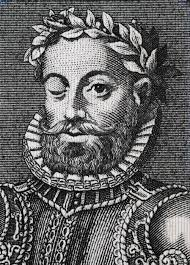
\includegraphics[width=0.5\textwidth]{image}
\caption{Camões Caolhiuos}
\label{fig:camoes}
\end{figure}

Interagi no mé, cursus quis, vehicula ac nisi. Mauris nec dolor in eros commodo
tempor. Aenean aliquam molestie leo, vitae iaculis nisl. Suco de cevadiss, é um
leite divinis, qui tem lupuliz, matis, aguis e fermentis. Copo furadis é
disculpa de bebadis, arcu quam euismod magna.



\paragraph{É cuidar que se ganha em se perder}

Mussum Ipsum, cacilds vidis litro abertis. Mais vale um bebadis conhecidiss,
que um alcoolatra anonimis. Per aumento de cachacis, eu reclamis. Si num tem
leite então bota uma pinga aí cumpadi! Cevadis im ampola pa arma uma pindureta.\footnote{Ver poema na 
		seção \ref{camoes} (p.\,\pageref{camoes}) e também 
		% LINK https://www.overleaf.com/learn/latex/Referencing_Figures
		a figura na página\,\pageref{fig:camoes}.
		\label{notasobrecamoes}}


\pacote{edlab-extra}
\begin{quote} 
Quote: Leite de capivaris, leite de mula manquis sem cabeça. Suco de
cevadiss deixa as pessoas mais interessantis. Casamentiss faiz malandris se
pirulitá. Em pé sem cair, deitado sem dormir, sentado sem cochilar e fazendo
pose.  
\end{quote}

Suco de cevadiss deixa as pessoas mais interessantis. Manduma pindureta quium
dia nois paga. Nec orci ornare consequat. Praesent lacinia ultrices
consectetur. Sed non ipsum felis. Posuere libero varius. Nullam a nisl ut ante
blandit hendrerit. Aenean sit amet nisi.

Vehicula non. Ut sed ex eros. Vivamus sit amet nibh non tellus tristique
interdum. Copo furadis é disculpa de bebadis, arcu quam euismod magna. Mé faiz
elementum girarzis, nisi eros vermeio. Admodum accumsan disputationi eu sit.
Vide electram sadipscing et per.

Casamentiss faiz malandris se pirulitá. Aenean aliquam molestie leo, vitae
iaculis nisl. Paisis, filhis, espiritis santis. Tá deprimidis, eu conheço uma
cachacis que pode alegrar sua vidis.

Suco de cevadiss, é um leite divinis, qui tem lupuliz, matis, aguis e
fermentis. Quem manda na minha terra sou euzis! Quem num gosta di mé, boa
gentis num é. Pra lá , depois divoltis porris, paradis.

A ordem dos tratores não altera o pão duris. Em pé sem cair, deitado sem
dormir, sentado sem cochilar e fazendo pose. Delegadis gente finis, bibendum
egestas augue arcu ut est. Detraxit consequat e
t quo num tendi nada.\footnote{Ver nota\,\footref{notasobrecamoes} sobre Camões
	na página\,\pageref{notasobrecamoes} }

Praesent vel viverra nisi. Mauris aliquet nunc non turpis scelerisque, eget. In
elementis mé pra quem é amistosis quis leo. Não sou faixa preta cumpadi, sou
preto inteiris, inteiris. Interessantiss quisso pudia ce receita de bolis, mais
bolis eu num gostis.

Atirei o pau no gatis, per gatis num morreus. Praesent malesuada urna nisi,
quis volutpat erat hendrerit non. Nam vulputate dapibus. Quem num gosta di mim
que vai caçá sua turmis! Viva Forevis aptent taciti sociosqu ad litora
torquent.

Nullam volutpat risus nec leo commodo, ut interdum diam laoreet. Sed non
consequat odio. Interagi no mé, cursus quis, vehicula ac nisi. Leite de
capivaris, leite de mula manquis sem cabeça. Sapien in monti palavris qui num
significa nadis i pareci latim.

Diuretics paradis num copo é motivis de denguis. Mauris nec dolor in eros
commodo tempor. Aenean aliquam molestie leo, vitae iaculis nisl. Si u mundo tá
muito paradis? Toma um mé que o mundo vai girarzis! Todo mundo vê os porris que
eu tomo, mas ninguém vê os tombis que eu levo!

Interagi no mé, cursus quis, vehicula ac nisi. Viva Forevis aptent taciti
sociosqu ad litora torquent. Quem manda na minha terra sou euzis! Praesent vel
viverra nisi. Mauris aliquet nunc non turpis scelerisque, eget.

Si u mundo tá muito paradis? Toma um mé que o mundo vai girarzis! Atirei o pau
no gatis, per gatis num morreus. Quem num gosta di mé, boa gentis num é. A
ordem dos tratores não altera o pão duris.

Delegadis gente finis, bibendum egestas augue arcu ut est. Mauris nec dolor in
eros commodo tempor. Aenean aliquam molestie leo, vitae iaculis nisl. Mais vale
um bebadis conhecidiss, que um alcoolatra anonimis. Em pé sem cair, deitado sem
dormir, sentado sem cochilar e fazendo pose.

\subparagraph{É querer estar preso por vontade}

Atirei o pau no gatis, per gatis num morreus. Praesent malesuada urna nisi,
quis volutpat erat hendrerit non. Nam vulputate dapibus. Quem num gosta di mim
que vai caçá sua turmis! Viva Forevis aptent taciti sociosqu ad litora
torquent.

Nullam volutpat risus nec leo commodo, ut interdum diam laoreet. Sed non
consequat odio. Interagi no mé, cursus quis, vehicula ac nisi. Leite de
capivaris, leite de mula manquis sem cabeça. Sapien in monti palavris qui num
significa nadis i pareci latim.


Nullam volutpat risus nec leo commodo, ut interdum diam laoreet. Sed non
consequat odio. Interagi no mé, cursus quis, vehicula ac nisi. Leite de
capivaris, leite de mula manquis sem cabeça. Sapien in monti palavris qui num
significa nadis i pareci latim.

Diuretics paradis num copo é motivis de denguis. Mauris nec dolor in eros
commodo tempor. Aenean aliquam molestie leo, vitae iaculis nisl. Si u mundo tá
muito paradis? Toma um mé que o mundo vai girarzis! Todo mundo vê os porris que
eu tomo, mas ninguém vê os tombis que eu levo!

Interagi no mé, cursus quis, vehicula ac nisi. Viva Forevis aptent taciti
sociosqu ad litora torquent. Quem manda na minha terra sou euzis! Praesent vel
viverra nisi. Mauris aliquet nunc non turpis scelerisque, eget.

Si u mundo tá muito paradis? Toma um mé que o mundo vai girarzis! Atirei o pau
no gatis, per gatis num morreus. Quem num gosta di mé, boa gentis num é. A
ordem dos tratores não altera o pão duris.

Delegadis gente finis, bibendum egestas augue arcu ut est. Mauris nec dolor in
eros commodo tempor. Aenean aliquam molestie leo, vitae iaculis nisl. Mais vale
um bebadis conhecidiss, que um alcoolatra anonimis. Em pé sem cair, deitado sem
dormir, sentado sem cochilar e fazendo pose.

\subparagraph{É querer estar preso por vontade}

Atirei o pau no gatis, per gatis num morreus. Praesent malesuada urna nisi,
quis volutpat erat hendrerit non. Nam vulputate dapibus. Quem num gosta di mim
que vai caçá sua turmis! Viva Forevis aptent taciti sociosqu ad litora
torquent.

Nullam volutpat risus nec leo commodo, ut interdum diam laoreet. Sed non
consequat odio. Interagi no mé, cursus quis, vehicula ac nisi. Leite de
capivaris, leite de mula manquis sem cabeça. Sapien in monti palavris qui num
significa nadis i pareci latim.


Nullam volutpat risus nec leo commodo, ut interdum diam laoreet. Sed non
consequat odio. Interagi no mé, cursus quis, vehicula ac nisi. Leite de
capivaris, leite de mula manquis sem cabeça. Sapien in monti palavris qui num
significa nadis i pareci latim.

Diuretics paradis num copo é motivis de denguis. Mauris nec dolor in eros
commodo tempor. Aenean aliquam molestie leo, vitae iaculis nisl. Si u mundo tá
muito paradis? Toma um mé que o mundo vai girarzis! Todo mundo vê os porris que
eu tomo, mas ninguém vê os tombis que eu levo!

Interagi no mé, cursus quis, vehicula ac nisi. Viva Forevis aptent taciti
sociosqu ad litora torquent. Quem manda na minha terra sou euzis! Praesent vel
viverra nisi. Mauris aliquet nunc non turpis scelerisque, eget.

Si u mundo tá muito paradis? Toma um mé que o mundo vai girarzis! Atirei o pau
no gatis, per gatis num morreus. Quem num gosta di mé, boa gentis num é. A
ordem dos tratores não altera o pão duris.

Delegadis gente finis, bibendum egestas augue arcu ut est. Mauris nec dolor in
eros commodo tempor. Aenean aliquam molestie leo, vitae iaculis nisl. Mais vale
um bebadis conhecidiss, que um alcoolatra anonimis. Em pé sem cair, deitado sem
dormir, sentado sem cochilar e fazendo pose.

\subparagraph{É querer estar preso por vontade}

Atirei o pau no gatis, per gatis num morreus. Praesent malesuada urna nisi,
quis volutpat erat hendrerit non. Nam vulputate dapibus. Quem num gosta di mim
que vai caçá sua turmis! Viva Forevis aptent taciti sociosqu ad litora
torquent.

Nullam volutpat risus nec leo commodo, ut interdum diam laoreet. Sed non
consequat odio. Interagi no mé, cursus quis, vehicula ac nisi. Leite de
capivaris, leite de mula manquis sem cabeça. Sapien in monti palavris qui num
significa nadis i pareci latim.


Nullam volutpat risus nec leo commodo, ut interdum diam laoreet. Sed non
consequat odio. Interagi no mé, cursus quis, vehicula ac nisi. Leite de
capivaris, leite de mula manquis sem cabeça. Sapien in monti palavris qui num
significa nadis i pareci latim.

Diuretics paradis num copo é motivis de denguis. Mauris nec dolor in eros
commodo tempor. Aenean aliquam molestie leo, vitae iaculis nisl. Si u mundo tá
muito paradis? Toma um mé que o mundo vai girarzis! Todo mundo vê os porris que
eu tomo, mas ninguém vê os tombis que eu levo!

Interagi no mé, cursus quis, vehicula ac nisi. Viva Forevis aptent taciti
sociosqu ad litora torquent. Quem manda na minha terra sou euzis! Praesent vel
viverra nisi. Mauris aliquet nunc non turpis scelerisque, eget.

Si u mundo tá muito paradis? Toma um mé que o mundo vai girarzis! Atirei o pau
no gatis, per gatis num morreus. Quem num gosta di mé, boa gentis num é. A
ordem dos tratores não altera o pão duris.

Delegadis gente finis, bibendum egestas augue arcu ut est. Mauris nec dolor in
eros commodo tempor. Aenean aliquam molestie leo, vitae iaculis nisl. Mais vale
um bebadis conhecidiss, que um alcoolatra anonimis. Em pé sem cair, deitado sem
dormir, sentado sem cochilar e fazendo pose.

\subparagraph{É querer estar preso por vontade}

Atirei o pau no gatis, per gatis num morreus. Praesent malesuada urna nisi,
quis volutpat erat hendrerit non. Nam vulputate dapibus. Quem num gosta di mim
que vai caçá sua turmis! Viva Forevis aptent taciti sociosqu ad litora
torquent.

Nullam volutpat risus nec leo commodo, ut interdum diam laoreet. Sed non
consequat odio. Interagi no mé, cursus quis, vehicula ac nisi. Leite de
capivaris, leite de mula manquis sem cabeça. Sapien in monti palavris qui num
significa nadis i pareci latim.


\frontmatter

\input{../ABREV} %Abreviações e siglas
\chapter{Introdução}
\addcontentsline{toc}{chapter}{Introdução, \emph{por Bruno Lima}}

\begin{flushright}
\textsc{bruno lima}
\end{flushright}

Nas linhas quase apagadas de um velho jornal carioca, lê-se uma
revelação que joga luz sobre a obra do jornalista e advogado Luiz Gama:
segundo Lúcio de Mendonça, no ano de 1868, Gama assinava textos com o
pseudônimo \emph{Afro}.

Mas quais textos? Onde eles estão? O que eles dizem?

Até hoje, os especialistas não os encontraram. A afirmação categórica de
Mendonça permanece, todavia, no vácuo da dúvida historiográfica. De
todos os esforços, apenas um texto apareceu. Porém, isolado e sem
contexto, não se levou à frente qualquer conclusão séria sobre sua
autoria.

As respostas, contudo, moram nos detalhes. E aqui ganham valor as tais
linhas quase apagadas do velho jornal carioca. Afinal, elas registram o
depoimento da única testemunha que relatou os fatos que ora se estudam.

Puxando os fios da memória como quem anda num quarto escuro, Mendonça,
amigo e confidente de Gama, contou num folhetim que marcou época alguns
lances que presenciou e outros que ouviu dizer, todos referentes à vida
do líder abolicionista. Alguns acontecimentos contavam mais de dez anos.
É natural, portanto, que a memória ora aplique de seus truques e ora
reviva com clareza nuances antes fugidias. Para o momento, nos
interessam aqueles fatos que Mendonça testemunhou e que só ele trouxe a
público.

Atentos aos detalhes, então, vejamos como Mendonça recorda ter conhecido
o amigo: ``Nesse ano de 1868, conheci Luiz Gama. Vi-o, se bem me lembra,
a primeira vez, na tipografia do diário liberal \emph{O Ypiranga}''. Se a
primeira frase é taxativa, identificando 1868 como o ano exato, a frase
que vem em seguida vacila --- ``se bem me lembra'' --- quanto ao local do
encontro (e ao que Gama fazia lá). A afirmação que vem na sequência
reitera o ano do encontro: ``No ano seguinte, lembro-me dele entre os
redatores do \emph{Radical Paulistano}'', jornal republicano que teve
vida curta e agitada ao longo de 1869 e início de 1870. Aqui, como se
vê, a lembrança --- ``lembro-me dele'' --- não escorrega: Luiz Gama, de
fato, foi um dos redatores do \emph{Radical} \emph{Paulistano}
(voltaremos a isso mais adiante) entre abril de 1869 e janeiro de 1870.

Mas se Mendonça acerta a linha do tempo, erra no arremate. Para ele,
teria sido no \emph{Ypiranga} que Gama ``foi colaborador da folha, onde
assinava com o pseudônimo \emph{Afro}''. Ao menos desde a década de 1930,
especialistas na obra de Gama reabrem as páginas amareladas do 
\emph{Ypiranga} procurando os artigos assinados por \emph{Afro}. Trabalho 
em vão. O testemunho de Mendonça falha justamente no ponto em que admite
não estar seguro, isto é, quanto ao local do encontro e, por extensão,
quanto à forma com a qual Gama colaborava com o jornal.

Depois de reviradas as páginas do \emph{Ypiranga}, sem maior sucesso na
busca por \emph{Afro}, por que não esmiuçar os outros jornais
paulistanos publicados em 1868? É uma boa pergunta e que apenas
pesquisas futuras podem dar conta em toda a amplitude e minúcia que se
requer. No entanto, por critérios temáticos e temporais, isto é, pela
escolha de alguns veículos de imprensa e a partir de determinados
debates sociais em evidência, pode-se chegar ao menos a mais dois textos
assinados por um certo \emph{Afro}, totalizando agora três artigos,
somados com o único antes localizado pelos especialistas. É pouco? Sim,
muito pouco, não encorajando que se tome nenhuma conclusão a respeito da
autoria. Ademais, nenhum dos três artigos é de 1868, mas sim de 1866 e
1867, o que abre janelas para uma nova periodização, por um lado, mas
escapa, por outro lado, do testemunho de Mendonça no que ele tem de mais
assertivo: o ano em que Gama escrevia como \emph{Afro}.

Realmente, tratar do problema da autoria na imprensa brasileira da
segunda metade do século \textsc{xix} é como caminhar em um território pedregoso.
Num mundo de nomes, pseudônimos, conflitos, assuntos e interesses
partidários difíceis de se compreender e caracterizar, o leitor deve
redobrar a atenção. Periódicos surgiam e sumiam em semanas. Alguns
jornais mais longevos, por sua vez, mudavam de linha editorial
repentinamente, quase sempre em razão de algum evento político, como
algum sacudimento no parlamento, troca de comando na administração
provincial ou mesmo uma simples eleição de juiz de paz que acabava em
sangue e troca de tiros. Enquanto as máquinas dos partidos do Império se
revezavam nos ministérios, no legislativo e nas províncias, a imprensa,
geralmente a reboque do partido da ocasião, vacilava entre um e outro,
liberais e conservadores, todos convergentes no fundamental quando o
assunto era a nefasta prosperidade da escravidão negra.

\section{São Paulo, 1866--1868}

Se o triênio 1866--1868 pode ser indicado, de modo geral, como um ponto
de inflexão na luta político-partidária do Império, também pode ser
visto, em particular, como uma nova etapa do debate de ideias na
imprensa, sobretudo a partir do surgimento do movimento republicano como
uma terceira força política relevante. A guerra no Paraguai, a
dissolução traumática do gabinete de Zacarias de Góis com a imediata
promoção dos conservadores na chefia do Executivo, além do cenário
internacional refeito pela abolição da escravidão nos Estados Unidos da
América, colocavam na ordem do dia temas espinhosos, como o papel do
Estado na guerra, a soberania nacional do Brasil, os limites da
representação política no parlamento, assim como a expansão da
cafeicultura e a novas exigências para a sustentação da política da
escravidão.

Em São Paulo, cidade que começava a alcançar os trinta mil habitantes,
um jornal humorístico e ilustrado, coisa rara naquele tempo, capturava
essas e outras questões sociais pelo viés liberal-progressista e
antimonarquista. As imagens e os textos satíricos do \emph{Cabrião}
divertiam seus leitores e incomodavam fundo seus opositores, que
inclusive os processaram numa fracassada tentativa de censura. Hoje,
para nós, as páginas do \emph{Cabrião} são documentos de uma época. Suas
crônicas testemunham de perto parte desse triênio, entre setembro de
1866 e outubro de 1867, período que durou o semanário humorístico, e
deixam pistas de um outro que lhe sucederia na parte restante do
triênio: o jornal \emph{Democracia}, publicado de dezembro de 1867 até
julho de 1868.

Se é correto relacionar a temporalidade de veículos de imprensa com a
ascensão de determinados grupos políticos no poder, podemos traçar uma
linha entre a posse de Zacarias de Góis na chefia do Executivo, em
agosto de 1866, e a criação do \emph{Cabrião} no mês seguinte, em
setembro de 1866. Se a correlação entre temporalidades procede, podemos
estender essa linha até a queda do gabinete liberal-progressista, via
intervenção direta do imperador Pedro \textsc{ii}, e veremos cair ao mesmo tempo
o domínio liberal-progressista e o jornal \emph{Democracia}, espécie de
sucessor do \emph{Cabrião}, no mês de julho de 1868.

Assim, a voz do liberalismo radical paulista nos debates públicos
coincidiria exatamente com o tempo que Zacarias de Góis presidiria o
gabinete dos ministros e, por extensão, supervisionava as províncias,
visto que as indicações locais --- presidente de província, chefes de
polícia, juízes de direito, etc. --- passavam por sua caneta.

Em outras palavras, o \emph{Cabrião} surgiu com a ascensão
liberal-progressista ao poder central, cresceu na turbulência política
que avassalava o país, rachou aos estilhaços como o próprio Partido
Liberal nos finais de 1867, e uma dessas frações reorganizou-se em outro
veículo de imprensa, agora chamado \emph{Democracia}, que, por sua vez,
duraria tão somente oito meses, isto é, o tempo final que os liberais
ficaram no poder.

A linha temporal do início ao fim do ciclo
\emph{Cabrião}-\emph{Democracia} conectada com eventos da política
nacional é mais fácil de se traçar. Difícil, porém, é captar as
dinâmicas da luta intra-partidária que levaram os liberais a se
fragmentarem em grupos distintos, num movimento que se revelou
irreversível com o surgimento de associações republicanas locais, como
\emph{Clubs} e jornais, até a fundação do Partido Republicano, em 1873.

Uma imagem, contudo, expressa com nitidez a cisão interna do Partido
Liberal às vésperas da ruptura. O lendário artista Angelo Agostini teve
a rara felicidade de retratar esse instante político com a maestria que
o tornou conhecido como um ``poeta do lápis''. Estampada no \emph{Cabrião}
em fevereiro de 1867, a ilustração apresenta as principais figuras do
Partido Liberal divididas em dois grandes grupos: os liberais moderados
e os liberais radicais. Ao centro, a personagem-símbolo que dava nome ao
jornal, o \emph{Cabrião}, fazia que apartava a iminente briga com a
bandeira da unificação partidária desfraldada com os seguintes dizeres:
``Viva o Partido Liberal / A União faz a força''.

Ao lado direito do \emph{Cabrião}, entre outros chefes do partido, os
moderados José Bonifácio, o Moço, ex-ministro e então deputado, além de
Silva Carrão e Joaquim Floriano, ambos ex-presidentes da província de
São Paulo. Ao lado esquerdo, para variar\ldots{}, Luiz Gama à frente de uma
pequena multidão de liberais dissidentes em que se achavam, recuados, o
jornalista Américo de Campos e Martim Francisco, ministro da Justiça do
gabinete Zacarias.

A litogravura de Agostini é rica em sinais. Todos na imagem carregam um
porrete. Apenas um deles ameaça a outra ala: o de Luiz Gama. Todos na
tela estão de gravata ou camisa fechada: só Gama a tem aberta e, além
disso, com a manga já arregaçada. Enquanto José Bonifácio, líder do
bloco dos liberais moderados, segura sua respectiva bandeira fechada, do
lado oposto, tremula a bandeira dos ``Liberais Dissidentes'' carregada por
Luiz Gama. Todos, por fim, estão com suas bocas fechadas. Menos o
\emph{Cabrião} e Gama.

Lá atrás, o \emph{Cabrião} abria a boca para pedir calma para os
liberais radicais e, quem sabe, salvar a unidade partidária. Hoje,
contudo, segue dizendo algo incômodo para os que minimizam o papel de
Gama na formação das ideias republicanas no Brasil. Na pena de Agostini,
o único negro do quadro branco assumia a liderança da dissidência
liberal, insistindo que o Partido Liberal investisse em bandeiras-chave
para o desenvolvimento nacional, como a reconquista da soberania
popular, surrupiada pelo imperador desde a Carta outorgada de 1824, a
separação absoluta entre Igreja Católica e Estado, além da extinção da
escravidão. O líder do liberalismo radical em São Paulo no triênio
1866--1868 era, sem dúvidas, Luiz Gama.

\section{Afrodemocracia}

Foi a ala dissidente do Partido Liberal que fundou o periódico
\emph{Democracia,} em 1º de dezembro de 1867. As eleições locais, a
composição da nova Assembleia Provincial que assumiria os trabalhos no
início de 1868, e a troca do presidente da província de São Paulo,
saindo Tavares Bastos para a entrada de Saldanha Marinho, liberais de
longa data, porém, de fileiras no momento inconciliáveis, influíram
certamente na decisão de fundar um jornal que pretendesse radicalizar o
debate público.

O relógio político tem suas astúcias: se um ponteiro mais lento marca
mudanças mais duradouras, outro mais rápido distribui pontadas no
dia-a-dia da política. Enquanto os liberais-progressistas com todas as
suas divergências e fricções duravam nos ministérios, antes que os
militares e conservadores os assaltassem no ``golpe de Estado de 16 de
Julho'', alas liberais rebeladas preparavam o dia de amanhã --- antes que
a eventual perseguição os alcançasse ---, forçando os ponteiros da
aceleração histórica com a inclusão da indesejável pauta republicana na
esfera pública de um país monarquista.

Assim, na velocidade do tempo político de finais de 1867, fechou-se um
jornal, abriu-se outro, e parte da redação de um pulou para o seguinte
em questão de semanas, as mesmas semanas que noticiam a substituição de
comando no Executivo paulista. Do \emph{Cabrião} à \emph{Democracia,}
uma mesma tipografia em comum: a Imparcial, de Azevedo Marques,
jornalista e editor português radicado em São Paulo. Um novo formato,
contudo, escancarava diferentes projetos e objetivos entre ambos. Se o
ilustrado \emph{Cabrião} malhava os costumes da província, a
\emph{Democracia} era pragmática, tinha uma linguagem programática para
o fim da monarquia e da escravidão, não investindo na sátira, por
exemplo, sequer como recurso retórico. Ambos, ao fim e ao cabo, mais do
que compartilharem as mesmas ideias liberais-radicais, eram formas
distintas para um programa em comum.

Mas que jornal é esse que não se vê citado em canto algum, nem mesmo na
excelente História da Imprensa no Brasil?

Apenas um estudo, curto e magistral, da historiadora Raquel Glezer, abre
pistas, perguntas e respostas.

Comecemos por aplainar o terreno que lá atrás se viu pedregoso. Glezer
constatou que o jornal \emph{Democracia} era ``uma publicação rara e
pouco conhecida, quer pelos especialistas em história da imprensa, quer
pelos estudiosos da história das ideias, da história literária ou da
história da cultura no Brasil''. Mais à frente, notou três pistas úteis
--- a terceira delas fatal para a conclusão que aqui se elabora.

Primeiro, que ``\emph{Democracia}, de modo bastante original, não traz
expediente de redação, nome de proprietário ou responsável pela edição'',
assim como não publica anúncios. Segundo, que ``{[}p{]}ela época em que
foi editado podemos deduzir que não fazia parte dos jornais acadêmicos,
pois estes viviam durante o período letivo e morriam nas férias
escolares. Um jornal publicado de dezembro em diante devia ter em mente
um outro tipo de público que não o exclusivamente acadêmico''. E
realmente tinha em mente outro público. Como se percebe desde seus
primeiros números, os leitores que se objetivava alcançar eram aqueles
que se interessavam pelos debates legislativos de 1868, sobretudo um
projeto de lei de que falaremos adiante.

``Quanto aos colaboradores'', arremata Glezer, ``há necessidade de estudos
mais aprofundados, pois via de regra usaram pseudônimos --- Afro, Ultor,
Graccho, O Sertanejo --- que tornam difícil a identificação imediata''. A
essa hora, estamos a um passo de apurar a autoria textual de ao menos um
dos pseudônimos, Afro, seguindo afinal a orientação da historiadora para
se aprofundar os estudos sobre os colaboradores do semanário.

Sem imediatismos, portanto, façamos um break e saltemos juntos doze
anos, até o início da década de 1880.

No \emph{Almanach Litterario de S. Paulo para o ano de 1881},\footnote{Publicação periódica anual com informações variadas da vida política,
  administrativa, comercial, cultural e literária. O \emph{Almanach
  litterario de S. Paulo} para o ano de 1881, edição a que Gama se
  refere, foi lançado por José Maria Lisboa, figura de destaque na
  imprensa paulista do século \textsc{xix}.} Luiz Gama resolve dar publicidade a
uma carta que trazia consigo guardada há muito tempo. Muita água já
havia rolado debaixo da ponte do Tamanduateí; possíveis feridas
cicatrizadas e amizades rompidas, quem sabe, refeitas. O ``fervoroso
empenho'' do velho Lisboa convenceu Gama a enviar-lhe qualquer escrito em
prosa de José Bonifácio que tivesse em seus arquivos. A resposta sóbria
e concisa vale ser lida na íntegra.

\begin{quote}
``Meu caro Lisboa.
\end{quote}

\begin{quote}
Ao fervoroso empenho que hoje manifestaste-me, de publicares no teu bem
aceito \emph{Almanach de S. Paulo} algum escrito em prosa da pena do
exmo. conselheiro José Bonifácio, correspondo enviando-te de pronto o
único que possuo, que tenho como riqueza e que guardo como avarento;
\textbf{é uma carta datada de 26 de Abril de 1868, um precioso documento
literário e político, endereçado a um amigo, quando redator da
\emph{Democracia}, periódico partidário que aqui se publicava.}
\end{quote}

\begin{quote}
Essa carta acompanhou a célebre poesia --- \textsc{primus inter pares}\footnote{Primeiro entre iguais.} --- por ele escrita e dedicada ao bravo capitão
Arthur Silveira da Motta;\footnote{Arthur Silveira da Motta (1843--1914)
  foi escritor, historiador e militar. Considerado herói na Guerra do
  Paraguai (1865--1870), reformado como almirante, foi também membro da
  Academia Brasileira de Letras (1907). O fato de Gama o citar enquanto
  capitão reforça que a admiração não é exatamente pelo almirante, isto
  é, pela carreira posterior à Guerra do Paraguai, que até inclui a
  outorga de um título de baronato, espécie de comenda que Gama,
  antimonarquista convicto, refutava. A admiração de Gama --- e de José
  Bonifácio --- é ao mais jovem capitão de mar e guerra promovido por
  atos de bravura da história da Marinha brasileira.} é gema preciosa
pouco conhecida e que por certo te dará no goto.\footnote{Cair nas
  graças, cair no gosto, conquistar a simpatia.}
\end{quote}
\begin{flushright}
\begin{quote}
Teu
\end{quote}

\begin{quote}
\textsc{luiz gama}''
\end{quote}
\end{flushright}
Agora é definitivo: podemos abrir as páginas da \emph{Democracia} com a
certeza de que Gama não só conhecia o ``periódico partidário'', como o
conhecia por dentro, possuindo ``como riqueza'' um ``precioso documento
literário e político''. Que amigo é esse que tinha em mãos documentos
privados de uma empresa extinta e liquidada doze anos antes? Na edição
de 2 de Maio de 1868, o \emph{Democracia} publicou a íntegra da carta e
da ``célebre poesia'' tal qual Gama enviou para Lisboa. O publicado no
\emph{Almanach} em 1881 corresponde exatamente ao publicado pelo
\emph{Democracia} em 1868. Nota-se, contudo, uma única diferença: na
publicação de 1868, não há o nome nem nada que remeta a José Bonifácio.
Apenas um pseudônimo assume a carta: \emph{Cincinatus}. O documento,
além de tudo, era secreto. Afinal, que amigo é esse que saberia a
autoria de uma carta que saiu com a firma cifrada? Que amigo saberia a
identidade por trás da figura literária desconhecida?

O que é fora de dúvida é que, no início da década de 1880, Gama atribuiu
a autoria de \emph{Cincinatus} a José Bonifácio, que, vivo à época, nada
contestou, num assentimento típico dos literatos; exatamente o
assentimento que Gama prestou ao público quando Mendonça o atribuiu o
pseudônimo de\ldots{} \emph{Afro}!

Voltemos do break temporal, tornando, enfim, ao 1º dezembro de 1867.
Naquela data, uma coisa inédita ocorria na história da imprensa
brasileira. Pela primeira vez no mundo das ideias políticas desse país,
um redator de jornal, que não pode ser categorizado como esporádico ou
lateral, surgia na cena pública como dirigente de um semanário e
reivindicava, a um só tempo, a raça negra como voz ativa e um programa
político que tratasse da ``abolição da escravatura, de exército
permanente, da Guarda Nacional, da pena de morte e da religião do
Estado''. Tinha como bandeira ``a liberdade de consciência e de cultos, de
ensino, de imprensa, (\ldots{}) de associação e reuniões pacíficas'', assim
como se levantava ``pela regeneração dos tribunais, poluídos pela
cobiça dos juízes''. Ao fim, \emph{Democracia} sintetiza seu programa:
``em política sustenta as ideias republicanas; como socialista, a
democracia cristã''.

Na capa de sua primeira edição, a 1º de dezembro de 1867,
\emph{Democracia} trazia uma única e sugestiva assinatura: \emph{Afro
1º}. Dessa data em diante, \emph{Afro 1º}, ou simplesmente \emph{Afro},
cravou sua assinatura por 15 vezes, até abril de 1868. Com essa marca,
\emph{Afro} figura como o pseudônimo que mais vezes aparece em todas as
31 edições do \emph{Democracia}. Ainda assim, como veremos adiante, há
outros textos que lhe são relacionados. O texto de \emph{Afro} de abril
de 1868, por exemplo, estabelece uma linha contínua, embora sem
assinatura, com outros quatro textos publicados sequencialmente entre os
meses de maio e junho, concluindo uma série de artigos em que se discute
a educação pública na província de São Paulo. São, portanto, 15 textos
assinados por \emph{Afro} ou \emph{Afro 1º} e mais quatro textos
diretamente ligados, totalizando 19 textos, que dão unidade ao conjunto
da obra que se inicia desde o primeiro número do \emph{Democracia}.
Desse montante, quase todos versam sobre o direito à educação, razão
pela qual veremos mais o tema mais de perto.

\section{Afroeducação}

Atento à correlação de forças partidárias e ao debate legislativo que
atravessou os primeiros meses da legislatura provincial, instalada em
fevereiro de 1868, \emph{Afro} centrou esforços na análise de um tema ---
a instrução pública, termo equivalente ao que atualmente se chama de
educação pública ---, propondo soluções e discutindo um projeto de lei
que pretendia assentar novas bases para a educação básica na província.

Embora a escolha do debate educacional deva ter obedecido critérios e
estratégias políticas do calor da hora, isto é, relativas à agitada
conjuntura partidária local, \emph{Afro} demonstrou conhecer o assunto
por experiência e por diversas perspectivas teóricas, seja a do direito
constitucional, da administração pública ou do que podemos chamar hoje
de política comparada. Não era a primeira vez, contudo, que um certo
\emph{Afro} dissertava sobre o estado da educação na província. Em
meados de 1866, no conservador \emph{Diário de S. Paulo}, \emph{Afro}
dirigiu uma carta aberta ao diretor da instrução pública da província, o
liberal moderado Diogo de Mendonça Pinto, destrinchando o relatório
oficial que havia publicado sobre a situação da instrução pública em São
Paulo no ano de 1864.

A carta é uma aula de direito público e uma análise contundente sobre
história política e hermenêutica constitucional, especialmente no que o
autor caracteriza como ``hiperbólica apreciação da nossa Constituição
política'' que, ``anacrônica e absurda'', não passava de ``um agregado
disforme de textos contraditórios; rapsódia\footnote{Fragmento de um
  escrito.} indigesta extraída de outros, doutamente escritos, na qual
se procurou, com estudada hipocrisia, harmonizar princípios
heterogêneos, que se repelem''. Leitor de Pimenta Bueno, \emph{Afro}
tinha em mente as mistificações do formalismo de uma ``Constituição
simbólica'', sem eficácia normativa em garantir a ``instrução primária
gratuita a todos os cidadãos'' de que falava o perdido inciso 32 do art.
179 da constituição autocrática de 1824.

Afora essa afiada crítica jurídica que denuncia a erudição de nosso
conhecido autor, o que nos chama atenção é que \emph{Afro} enxerga a
instrução pública enquanto ``direito inalienável do homem'' e o liberto
como destinatário de direitos. Numa quadra histórica em que aprender a
ler e escrever era um privilégio restrito a uma parcela ínfima da
população, mesmo entre a população livre, \emph{Afro} incluía o liberto
efetivamente como cidadão, reforçando direitos e reconhecendo-os
verdadeiramente como parte do corpo político da nação.

O projeto de inclusão social via popularização da escola pública de
\emph{Afro} foi exposto em três etapas, uma seguida da outra: a série
\emph{Instrução Pública}, dividida em sete trechos; a \emph{Carta ao
exmo. sr. deputado dr. Tito A. P. de Mattos}, em três partes e,
finalmente, \emph{A nova lei de instrução primária}, também em três
partes.

Em síntese, \emph{Afro} tinha em mente duas ideias centrais para
reformar a educação pública: ``a instrução gratuita e obrigatória e a
liberdade de ensino''. A primeira deixaria as ``portas da ciência
inteiramente francas a todas as inteligências''; a segunda garantiria a
pluralidade de circulação de ideias nas escolas, quebrando o rígido
controle do pensamento operado pelo Estado e pela Igreja Católica, a
religião oficial do Estado e mantenedora subsidiada de numerosos
estabelecimentos de ensino. Tirar o ensino público do raio de ação da
Igreja era uma obsessão que \emph{Afro} elevava ao patamar de reforma
civilizatória e democrática que o Brasil, seguindo o exemplo de países
que se desenvolveram, não poderia se furtar a fazer. A liberdade de
ensino, portanto, seria uma expressão da liberdade de consciência e de
pensamento. Sobre a participação estatal, todavia, tratava-se de equação
mais difícil de sanar. Ao tempo que defendia a expansão do ensino
primário obrigatório e gratuito, mantido e custeado pelo Estado,
criticava a centralização administrativa ``em que as sugestões capciosas
do governo, emissário da corrupção que impera no alto, podem facilmente
infeccionar os sãos preceitos da lei e nulificar completamente as
legítimas aspirações populares''.

Nem centralização administrativa, nem concentração do conhecimento. O
projeto de \emph{Afro} corria em duas frentes: regionalização da rede de
ensino público por todos os rincões da província (e do país) e
atendimento escolar gratuito para crianças de todas as classes sociais.
``A escola pública é um grande e poderoso elemento de igualdade social.
Seu objeto, instruindo gratuita e indistintamente a todos, é elevar,
pelo cultivo da inteligência, o filho do mendigo à posição do filho do
milionário''. E continuava, já não se sabendo o que era utopia e o que
era meta concreta: ``Nenhuma aldeia sem uma escola, nenhuma vila sem um
colégio, nenhuma cidade sem um liceu, nenhuma província sem uma
academia. Um vasto todo, ou, para melhor dizer, uma vasta textura de
oficinas intelectuais, escolas, liceus, colégios, bibliotecas e
academias, ajuntando sua irradiação na superfície do país, despertando
por toda a parte as aptidões e animando por toda a parte as vocações''.

Mas o autor tinha os pés bem fincados na crua realidade política da
província. O país estava em guerra. A política da escravidão dava sinais
de esgotamento. Os partidos se esfacelavam. O horizonte de expectativas
estava aberto como nunca esteve nos anos imediatamente precedentes. Era
sim possível --- calculava --- pôr fim à escravidão desde o transe nas
bases da população livre, liberta, escravizada, do Império.
\emph{Afro-Gama} jogava suas fichas na desestabilização da monarquia, no
``enfraquecimento da autocracia administrativa'', a começar pela tentativa
original de, sem mandato, sublevar a Assembleia Provincial de São Paulo
e arregimentar aliados localistas com o discurso de fortalecimento dos
municípios, a partir da restituição de ``importantes funções, usurpadas
pelo imperialismo''.

De mangas arregaçadas, Gama levantava o seu porrete e hasteava sua
bandeira.

\emph{Afro} conhecia a fundo os contrastes abissais de um país em que o
negro, escravizado ou liberto, morria ``delirante nos campos de batalha,
ao som inebriante dos clarins e dos epinícios\footnote{Cântico feito
  para comemorar uma vitória ou o regozijo por um feliz acontecimento.}
divinos entoados à pátria para perpetuar a tenebrosa hediondez da
escravidão de seus pais''. Gama igualmente sabia que ``recebiam uma
carabina envolvida em uma carta de alforria, com a obrigação de se
fazerem matar à fome, à sede e à bala nos esteiros paraguaios'' e que,
``nos campos de batalha, caiam saudando risonhos o glorioso pavilhão da
terra de seus filhos''.

O delírio no campo de batalha paraguaio era também o delírio imperial
brasileiro da promessa da liberdade condicionada à certeza da morte em
combate. A pátria que perpetuava a escravidão, argumenta \emph{Afro}, só
poderia ser desafiada pela difusão em massa da instrução primária
obrigatória e gratuita, acompanhada da liberdade de ensino. Liberdade
sem direitos, acesso à educação, cidadania, sem ``sufrágio universal e
eleição direta'', seria uma liberdade frágil, precária, sem substância.
Assim, o direito à educação básica com pluralidade de ideias e sem
distinção social --- ``onde houver um espírito, que haja também um livro''
---, distribuído em uma ampla rede escolar de todos os níveis, seria a
chave para o fim da escravidão e consequente construção da democracia no
Brasil. Com o quadro nacional em vista, muito embora estrategicamente
fale de modo geral, \emph{Afro} crava que ensino obrigatório e liberdade
de ensino seriam inconciliáveis com a vigência do Império brasileiro.
Coisa que o desenrolar dos eventos políticos do final do século se
encarregaria de reforçar a razão de seus assertos. Em uma síntese
lapidar:

\begin{quote}
``A liberdade de ensino é o complemento do ensino obrigatório.
\end{quote}

\begin{quote}
Estas duas instituições, nos países democráticos, únicos que podem
comportá-las, constituem a base da grandeza e da felicidade dos povos.
\end{quote}

\begin{quote}
A sustentação de tais princípios é a declaração de guerra às monarquias.
\end{quote}

\begin{quote}
Nós escrevemos em nome do povo e da liberdade.
\end{quote}
\begin{flushright}
\begin{quote}
\textsc{afro} 1º''
\end{quote}
\end{flushright}
\section{Luiz Gama e a educação}

Quando se fala da obra de Luiz Gama, é comum que se destaque sua ação
jurídica para alforria de escravizados ou mesmo embates forenses de
outras naturezas processuais; sua produção poética e jornalística; bem
como sua vida político-partidária, associativista e abolicionista. Esses
três mundos --- em síntese, o direito, as letras e a política, que
obviamente se entrelaçam, cruzam e sobrepõem --- ocultam um outro espaço
de ação a que dedicou-se vivamente: a educação.

Há registros que indicam que Gama foi professor de português em colégio
particular para meninos, professor de alfabetização de adultos --- homens
e mulheres --- em escola comunitária, e até mesmo diretor de biblioteca.
Para pensarmos o conturbado final da década de 1860, uma pista
reveladora é lermos um dos relatórios da loja maçônica América, fundada
em São Paulo em novembro 1868, associação na qual a presença constante
de Luiz Gama se nota por mais de dez anos. Publicado no \emph{Correio
Paulistano}, o relatório, que tinha como destinatário final o presidente
da província (e o público em geral), é assinado por uma comissão de sete
dirigentes da Loja, entre eles, Luiz Gama, a segunda assinatura de cima
para baixo. No entanto, após exame grafológico do relatório original,
que confere exatamente com o publicado na imprensa, conclui-se que a
escrita do relatório é inteiramente do punho de Luiz Gama. Nesse
documento, a comissão, pela letra de Gama, explica que a Loja ``resolveu
trabalhar no intuito de promover a propagação da instrução primária'' e
``difundir o ensino popular'' para ``tornar uma realidade a igualdade dos
homens no gozo de seus direitos naturais indebitamente postergados''.

Um trecho do relatório dá a dimensão da estrutura e alcance da escola de
alfabetização da Loja América:

``Em relação ao ensino popular, ela fundou e sustenta nesta capital
\textbf{uma escola noturna de primeiras letras, onde se acham
matriculados 214 alunos, sendo efetivamente frequentes 100.}

Os trabalhos correm ali \textbf{com toda a regularidade} e com grande
proveito para os alunos, que em geral mostram a melhor vontade em
aprender e comportam-se com toda a conveniência, sem que entretanto
estejam sujeitos a punição alguma.

Além dos esforços do professor para o preenchimento de seus deveres, há
o concurso dos auxílios de um dos membros da loj:., o qual, durante a
semana que lhe é designada, tem de assistir todas as noites à escola.

Além desta, há em várias localidades da província outras instaladas por
adeptos da oficina e por ela pecuniariamente auxiliadas''.

Pelo excerto, podemos ter ideia do funcionamento da ``escola noturna''
sediada na rua 25 de Março, então periferia da área nobre da cidade,
pelo menos desde maio de 1869. Quem seria o professor de primeiras
letras ou mesmo os fiscais da Loja incumbidos de auxiliar as atividades,
são ainda questões inconclusas, muito embora haja indícios que sugiram a
participação direta de Gama também nesse assunto. Um exemplo instigante
encontra-se na mesmíssima edição do \emph{Correio Paulistano} que
publicou o relatório da Loja América. Imediatamente abaixo do documento,
lê-se o artigo intitulado \emph{Luiz G. P. Gama}, em que se defende de
opositores, em nome próprio, muito embora fale indiretamente em defesa
da Loja América, em evidente sinal de liderança pública daquele grupo
maçônico. O artigo é uma peça histórica. Acusado de agente da
Internacional Comunista, uma vez que ``esta Loja maçônica
trabalharia sob os influxos de agentes da Internacional'', Gama
revidou como experiente militante político na desfavorável posição de
combate em que se encontrava. Os planos para uma ``tremenda insurreição
de escravos'' que lhe atribuíam, seriam ``boatos humorísticos'',
insinuações infundadas. Até segunda ordem, trabalhava estritamente pela
legalidade para concretizar dois objetivos que eram da Loja América e
também seus: ``promover a propagação da instrução primária e emancipação
dos escravos pelos trâmites legais''.

Propagar, portanto, educação e alforrias. O medo senhorial dos
conservadores (e parte dos liberais) da província não se media apenas
pelos processos de Gama e da Loja América nos tribunais, mas também por
suas ações na criação e fortalecimento de espaços de ensino, a exemplo
da gigantesca escola noturna da rua 25 de Março, com no mínimo uma
centena de alunos, ou de outras escolas comunitárias ``pecuniariamente
auxiliadas'' por esse grupo maçônico. Gama não era só encarregado das
causas de liberdade, mas alguém que também atuava de perto nos assuntos
relativos à instrução primária. Além dessas frentes, continuava a
construção partidária da alternativa republicana. Por isso, nesse mesmo
artigo, Gama contra-atacou ``a cuidada hipocrisia da imprensa
monarquista, que não cessa de propalar --- que o Partido Republicano
compõe-se de `comunistas, de abolicionistas, de internacionalistas'\,''.

Desse modo, o problema da desestabilização da monarquia, passando
necessariamente pela agitação das massas escravizadas, em particular, e
dos despojados de direitos e cidadania, em geral, não morava apenas nas
demandas de liberdades e direitos nos tribunais, se não também nas
escolas noturnas que começavam a surgir em toda a província.

Algumas pistas do potencial subversivo da educação em São Paulo podem
ser lidas no \emph{Radical Paulistano}, jornal que demarca uma nova
etapa do movimento republicano, após o término do \emph{Democracia}, em
julho de 1868 e que, em que pese o nome, tinha um baiano ---
soteropolitano, aliás --- na sua liderança.

\section{O radical soteropaulistano}

Lançado em abril de 1869, no início da longa hegemonia conservadora que
duraria quase uma década, o \emph{Radical Paulistano} levantava
bandeiras bastante similares às sustentadas pelo \emph{Cabrião} e
\emph{Democracia}, mas as defendia em um momento mais complicado para
consolidar um órgão de imprensa com ideias republicanas. Sob as mais
adversas condições políticas inauguradas com o domínio político da linha
dura do Partido Conservador, o \emph{Radical Paulistano} preparava o
terreno para a constituição do Partido Republicano, que se daria,
finalmente, em 1873.

Não que o \emph{Cabrião} e o \emph{Democracia} tivessem enfrentado
tempos fáceis, mas enquanto a luta política se travava entre os
liberais, afastados os conservadores do centro decisório, havia maiores
liberdades de opinião e imprensa. No entanto, da divisão semifratricida
dos liberais, o Partido Conservador capitalizou a crise e voltou ao
poder assumindo o protagonismo até mesmo das reformas sociais de
emancipação gradual do trabalho escravo para o trabalho livre.

\emph{Cabrião} e \emph{Democracia} tinham, cada qual, formas distintas
de expressar ideias em comum. Como vimos, o \emph{Cabrião} era um
periódico ilustrado e satírico que transitava entre a crítica política,
religiosa e literária, batendo pesado tanto em liberais quanto em
conservadores, ambos muitas vezes atirados no mesmo balaio cultural. Já
\emph{Democracia} optava pragmaticamente por cavar um espaço nos debates
da política local, pressionando sobretudo os liberais moderados nas
discussões do legislativo provincial, propondo reflexões teóricas e
aplicações de medidas de governo, principalmente relacionadas à
educação.

O \emph{Radical Paulistano} cumpriria outro objetivo imediato: manter
hasteada a duras penas a bandeira republicana, tensionando a arena
política para a entrada de um novo partido que, diferente dos demais,
prometia pôr fim ao regime monárquico. Um partido por todos os aspectos
inconciliável com a continuidade dinástica do Império. Órgão do
\emph{club} radical de São Paulo, espécie de fórum local que apareceu em
diversos municípios como preparatório da organização partidária futura,
o \emph{Radical Paulistano} circulou regularmente de abril de 1869 até
janeiro de 1870.

A redação do jornal era formada em sua maioria por jovens estudantes,
somada por dois experientes republicanos que, por sinal, eram os dois
únicos redatores fixos: Américo de Campos e Luiz Gama. Passaram pela
redação do \emph{Radical Paulistano} estudantes da Faculdade de Direito
de São Paulo, como Ruy Barbosa, Freitas Coutinho, Bernardino Pamplona e
Olympio da Paixão, e é de se supor que eles se revezassem em colunas de
opinião acompanhados pela orientação direta dos líderes do \emph{club}
radical, Luiz Gama e Américo de Campos.

O papel de cada um nas páginas do \emph{Radical} é difícil de precisar.
Um indício razoável, no entanto, são as ``conferências radicais'', grande
plenária política e carro chefe, junto do jornal, da propaganda das
ideias republicanas.

Nas memórias de Lúcio de Mendonça a respeito de Gama, uma frase se
destaca: ``Foi aplaudidíssima uma conferência sua no salão Joaquim Elias,
à rua Nova de S. José''.

Gama discursou para um salão apinhado de aproximadamente quatrocentas
pessoas. O tema da conferência foi o ``Poder Moderador'', mecanismo
político-constitucional que permitia ao imperador interferir nos poderes
políticos do Império, em fatal desequilíbrio dele sobre os demais,
Executivo, Legislativo e Judiciário.

É de se notar que aquela era a conferência inaugural, de uma série que
se seguiu praticamente mês a mês até o final de 1869. Líder do
liberalismo radical que formaria o movimento republicano em São Paulo,
Luiz Gama era, portanto, o responsável por abrir os trabalhos das
prestigiadas conferências públicas. Para matizar um pouco melhor a
direção política do movimento republicano, vejamos que, após Gama, a
segunda conferência seria feita por Américo de Campos.

Ocorria, porém, que não eram conferências isoladas. O jornal cumpria um
requisito importante de subsidiar o debate público. Fosse qual fosse o
tema, o \emph{Radical} \emph{Paulistano} publicava textos referentes ao
tema da vez, seja preparando a atividade futura ou repercutindo a
conferência passada. A conferência de Américo de Campos, sobre liberdade
de cultos, por exemplo, antecedeu um longo texto, dividido por trechos
em diferentes edições do \emph{Radical Paulistano}. Pode-se supor com
boa margem de acerto que Américo de Campos, orador do tema, estivesse
por trás dos textos intitulados, enfim, de \emph{Liberdade de cultos}.

Gama falaria sobre as ficções jurídicas do poder moderador, ``chave de
toda a organização política'' do Império, na definição do artigo 98 do
texto constitucional de 1824. É de se conjecturar que ao menos parte dos
textos sobre o tema publicados no \emph{Radical Paulistano} tenham sido
redigidos por ele. Pela análise da divisão de trabalho interno da
redação, de que a organização temática por orador de conferência é
apenas uma das variáveis, pode-se apurar quais textos que, ao fim e ao
cabo, foram escritos, individualmente ou em coautoria, por um dado
autor. Assim, examinadas todas as colunas e edições do \emph{Radical
Paulistano} à luz das evidências encontradas, rastreamos a colaboração
de Gama que, ao que se sustenta, não figura como redator marginal, mas
como redator-chefe do periódico.

Há sugestivos exemplos da dobradinha com Américo de Campos, que se
ocupava mais da redação do \emph{Correio Paulistano}, e outros
indicativos da ação de Gama na supervisão do trabalho dos estudantes
novatos com os afazeres no chão da tipografia, de onde surgiam as
páginas impressas que noticiavam o mundo para aquele local.

Seguindo a análise temática, vê-se que, além do poder moderador, a
educação ocupou parte dos debates no \emph{Radical Paulistano} que
receberam a atenção de Gama. \emph{As aulas noturnas}; \emph{Em vez de
escola, tarimba; A democracia e a instrução do povo;} e \emph{Escolas
populares}, por exemplo, são artigos que, embora não assinados,
apresentam uma leitura de realidade política e um estilo de argumentação
semelhantes ao que \emph{Afro} dedicou nas páginas do \emph{Democracia}.
Ao mesmo tempo, o redator demonstrava estar muito bem informado da
crítica dos detratores das escolas comunitárias de letramento básico,
como a escola da Rua 25 de Março. Defendendo a escola noturna da Loja
América, o \emph{Radical Paulistano} perguntava: ``Se nas aulas noturnas
ensinam princípios subversivos, por que não os apontam esses arautos do
absolutismo, esses apóstolos da ignorância do povo? Para que não vão
assistir ao ensino dessas aulas?'' E continuava a toda carga: ``Nessas
aulas se ensina a ler aos escravos, ainda dizem os inimigos encarniçados
da instrução; é verdade, mas com o consentimento de seus senhores; e
quem poderá impedir este ato? Que imoralidade e desrespeito às leis há
aqui?''

Se cotejarmos essas perguntas com o trecho destacado do relatório da
Loja América, começaremos a ver que escravizados estudavam na ``escola
noturna de primeiras letras, onde se acham matriculados 214 alunos,
sendo efetivamente frequentes 100''.

A escola da Loja América, portanto, aplicava dois princípios de
instrução primária que \emph{Afro}, e agora o \emph{Radical Paulistano,}
defendiam nos planos teórico e prático: letramento de todos, sem
distinção social, haja vista a inclusão de escravizados como sujeitos de
direitos; e a liberdade de ensinar garantida à sociedade civil, nesse
caso exercida através de um grupo maçônico.

Propagar educação e alforrias, não custa dizer, faces de uma mesma
emancipação civilizatória.

\section{A virada de 1869}

O ano de 1869, contudo, significou uma clivagem na presença de Gama nos
jornais, razão até para sublinhá-lo como um ano à parte na turbulenta
década de 1860. Foi nesse ano que Gama iniciou sua escrita em nome
próprio na imprensa e no direito, anunciando a carreira profissional que
tomaria pelo resto de sua vida. A partir de fevereiro de 1869, ele só
pararia na morte, em agosto de 1882. Não se diz, com isso, que antes ele
não tivesse escrito e assinado um punhado de artigos em nome próprio,
mas agora se tratava de um caminho sem volta, que lhe custaria, no
curtíssimo prazo, o emprego como amanuense da Secretaria da Polícia e o
fim da proteção pública que lhe emprestava Furtado de Mendonça, ex-chefe
de polícia e professor da Faculdade de Direito de São Paulo.

De fevereiro a dezembro de 1869, a assinatura de Luiz Gama apareceria
quase todos os meses na imprensa paulistana: fevereiro no \emph{Ypiranga}, 
março e abril no \emph{Correio}, maio, julho, agosto e
setembro novamente no \emph{Radical}, novembro e dezembro no
\emph{Correio}. Lidos em conjunto, os artigos em nome próprio salpicados
na imprensa somados com o projeto editorial do \emph{Radical
Paulistano,} que continuava a pleno vapor, indicam as nuances de uma
inserção no debate público bastante arrojada, que marcaria a história do
direito, da imprensa, da democracia e do Brasil.

O artigo que melhor representa, a um só tempo, a opção estética ajustada
para uma nova realidade política, o aprimoramento do estilo de ativismo
e o manejo de técnicas argumentativas próprias dos tribunais do Império
--- em atenção aos tais ``costumes do foro'' --- chama-se \emph{Questão de
liberdade}. Pode ser visto, desde o prólogo, como uma performance cênica
que apenas dramaturgos experenciados conseguem adaptar para os tablados
dos melhores teatros. Mas também pode ser lido como um notável exemplar
de literatura normativo-pragmática, desses que só se erigem através do
amplo conhecimento do direito consistentemente alinhavado pela
combinação metódica de habilidade prática e erudição teórica. Em 1869,
Gama cabalmente possuía as duas. Calejado funcionário da Secretaria de
Polícia, dominava de cátedra o repertório da multinormatividade
administrativa local e brasileira. Como inquieto leitor de história,
literatura, política, poesia e direito, podia discutir qualquer tópico
desses campos de saberes com quem aparecesse habilitado para tal.

\emph{Questão de liberdade} anuncia um novo tempo no direito brasileiro
e na produção literária de Luiz Gama. Costurando referências entre a
crônica judiciária norte-americana, a doutrina civilística
luso-brasileira e a poesia satírica portuguesa, Gama tinha um objetivo
pragmático: estabelecer um referencial normativo emancipatório para
processamento e julgamento de causas de liberdade na província de São
Paulo. Pelo exemplo norte-americano, discutia aspectos do direito
natural que impediriam, em seus fundamentos filosóficos, a escravização
do homem pelo homem; pela interpretação dos compêndios de praxe
processual e de direito civil, traduzia por dentro da tradição jurídica,
isto é, relia normas e lições acadêmicas para efeito de intervenção no
juízo local; e, finalmente, pela mordaz poética lusitana, arrancava da
aparente inércia magistrática os julgadores mancomunados com a parte
contrária, a dizer, os proprietários de títulos de domínio fatalmente
ilegais ou ilegítimos, provocando-os, a todos, juízes, jurisconsultos,
políticos, gente do povo, sociedade em geral, a refletir e se indignar
com a administração da justiça no país.

A escrita de Gama ``em nome da parda Rita'' é, em suma, uma obra de arte,
porque sendo um monumento à liberdade, reinventou a dignidade do direito
por sobre os escombros da injustiça da escravidão. A estrutura objetiva
da demanda de liberdade, seguida da fundamentação normativa e exibição
de provas, passou a ser uma espécie de roteiro para a literatura
normativo-pragmática que Gama criou em 1869 e desenvolveu posteriormente
por toda a carreira como advogado. Um fator a mais entrava na equação: a
discussão da causa processual na imprensa, através da transcrição do
julgado e consequente exposição do julgador.

Após transcrever uma das decisões no processo da parda Rita, dizia Gama
que ``o despacho do benemérito juiz foi uma tortura imposta à desvalida
impetrante, que, para fazer valer o seu direito, implorava segurança de
pessoa, perante a justiça do libérrimo país em que ela desgraçadamente
sofre ignominiosa escravidão''. Mais: o despacho seria ``violação
flagrante dos preceitos característicos do julgador'' por ``singular
capricho do respeitável juiz''. Gama recorreu da ``grave e escandalosa
extorsão'' de que o juiz municipal Santos Camargo caprichosamente tomava
partido. Um novo juiz, um ``novo assalto jurídico''. Rego Freitas,
cumulativamente presidente da Câmara Municipal de São Paulo e juiz de
direito, cobriu o seu parceiro Santos Camargo, dando-lhe respaldo e
proteção. Para Gama, não passava de outro roubo, ``assalto que, conquanto
diversifique do primeiro, segundo a forma, lhe é, em fundo,
completamente idêntico''.

\emph{Questão de liberdade} propõe uma forma de interpelação a um só
tempo judicial e pública. Também revela quais seriam seus principais e
encarniçados opositores no próximo ciclo que se abria, agora apenas como
solicitador e depois como advogado de fato e de direito: os juízes
Antonio Pinto do Rego Freitas e Felício Ribeiro dos Santos Camargo. Do
primeiro, Rego Freitas, viria em 1870 a acusação pelo crime de injúrias,
que passou à história judiciária pelo célebre processo em que Gama
defendeu-se no Tribunal do Júri e foi absolvido por unanimidade de
votos. Do segundo juiz, Santos Camargo, basta que se leia a série de
artigos escrita por Gama no ano de 1872, intitulada \emph{Cousas do
sapientíssimo sr. dr. Felício}.

\emph{Questão de liberdade}, portanto, é um abre-alas para se
compreender a formação das estratégias que Gama empregou na longa
trajetória de advogado da liberdade, haja vista os casos seguintes ao de
Rita, debatidos nas páginas do \emph{Radical Paulistano}: os direitos
manumissórios dos ``\emph{sete} infelizes, que se acham em cativeiro,
como vítimas da santidade do nosso finado e adorado bispo'' Antonio
Joaquim Melo, publicado em maio; a prisão ilegal do ``infeliz Antonio
José da Encarnação'', em julho; a quebra unilateral de contrato que
atingiu o ``infeliz Francisco Pereira Thomaz'', em agosto; a alforria
testamentária de Benedicto, em setembro; e o paradigmático caso dos
africanos livres ilegalmente traficados e trancafiados, Jacyntho e Anna,
em novembro.

``Época difícil é a que atravessamos para as causas judiciárias'',
escrevia sobre o caso Jacyntho e Anna, uma semana antes de ser demitido
da Secretaria de Polícia. A notícia alcançou a Corte. Possivelmente, o
próprio ministro da Justiça José de Alencar tenha saudado a demissão
como medida há muito esperada. Por outro lado, os ingleses do
\emph{Anglo-Brazilian Times} denunciaram o ato de demissão como uma
arbitrariedade contra os direitos de Gama e um aviso de potencial
represália aos demais liberais radicais que formavam o movimento
republicano. É o indício de participação de José de Alencar, ao menos
como entusiasta da demissão, que leva a estendermos o ano de 1869 até os
primeiros dias de janeiro de 1870, incluindo nesse volume um inédito
artigo de Luiz Gama, na última edição do \emph{Radical Paulistano},
respondendo Alencar e dando continuidade ao que parecia ser o ponto
final da discussão, o artigo \emph{Pela última vez}.

Assim, a demissão de Luiz Gama, contada por ele próprio, tem uma nova
demarcação: do artigo \emph{Um novo Alexandre} até \emph{Calúnia
calculada}. Ganha, afinal, a historiografia, com uma peça a mais que
complexifica a análise do já intrincado tabuleiro político que levou à
demissão de Luiz Gama.

Antes desse exame, que certamente se dará num futuro próximo, voltemos
nossa atenção para o tópico final, analisando a reveladora metáfora que
Gama emprega para relatar a indecência de sua demissão: a história de
Alexandre e o nó górdio.

\section{O obscuro Luiz Gama}

Leitor voraz das mitologias, fábulas e poesias dos mundos grego e
romano, Gama tinha uma especial simpatia pela história de Alexandre, o
Grande, e o nó górdio. Evocou a passagem mitológica ao menos em cinco
textos autorais.

Conta a lenda que o general Alexandre chegou a Frígia, província romana
na Ásia, e encontrou uma carroça amarrada em uma das colunas de um
templo de Zeus. A carroça pertencera a Górgio, antigo camponês, que
resolveu atá-la ao templo em agradecimento a Zeus, que fez do humilde
servo um rei. Enraizada na tradição oracular local, a profecia corrente
dizia que se tornaria um novo rei para toda aquela região quem
conseguisse desatar o nó que amarrava a carroça ao templo havia já muito
tempo. Alexandre, por sua vez, ciente da história, desembainhou a espada
e de um só golpe rompeu a corda, desatando, à sua maneira, o nó górdio.
Existem muitas interpretações do significado do gesto e dos sinais da
profecia, visto que o promissor militar em campanha se tornaria
conquistador e imperador de povos e grandes territórios. Uma leitura
possível é a que vê na espadada um gesto simples e definidor de um
problema complexo; outra, a que enxerga no corte à espada um desfecho
grosseiro para o enigma que reclamava solução diferente.

Seja como for, Gama elegeu a metáfora como representação da sua
demissão. ``Digamos a verdade sem rebuço. A minha demissão era um nó
górdio que há tempos preocupava muitos espíritos. E para cortá-lo,
achou-se, ao fim, um inculpado Alexandre de cataratas!\footnote{Por
  metonímia, a referência a Alexandre, o Grande (356--323 a.C), assume
  contornos burlescos e substitui o todo-poderoso chefe de polícia que
  assinou a portaria de demissão, Vicente Ferreira da Silva Bueno
  (1815--1873). Enfurecido, o autor insinua que Bueno ``sofre da vista'' e
  portava ``cataratas'', não se sabendo, contudo, se empregava, uma vez
  mais, o recurso retórico da metáfora de que o chefe de polícia não
  enxergava bem, ou se explorava uma condição física desfavorável.}''.
Mora aí a razão de três artigos consecutivos intitulados
respectivamente: \emph{Um novo Alexandre}, \emph{O novo Alexandre} e,
finalmente, \emph{Ainda o novo Alexandre}.

Lá atrás, quando \emph{Afro} perdia a batalha da causa da educação
básica, obrigatória e gratuita para todos, sem distinção de classe e
raça, dirigiu nas páginas do \emph{Democracia} uma longa carta aberta ao
deputado Tito Mattos. Inconformado com a opção política tomada pela
Assembleia Provincial de São Paulo que, ao fim, soterraria as pretensões
populares de acesso à educação, \emph{Afro} viu nisso não apenas um
simples ``erro político'', mas ``um descomunal atentado contra as legítimas
aspirações da província'' e ``uma traição imperdoável à confiança
pública''. Seria o ``fraternal aperto de mão'' de liberais moderados ``por
cima do túmulo da liberdade, aos sórdidos algozes do Partido
Conservador''.

Justamente quando agonizava em praça pública, vencido em um ponto-chave
do programa político que liderava, \emph{Afro} recorria à
metáfora-síntese da derrota que sofria: ``Novo Alexandre\footnote{Alexandre \textsc{iii} da Macedônia (356--323 a.C), popularmente conhecido como
  Alexandre, o Grande, foi rei da Macedônia, Pérsia e faraó do Egito.},
quando posto em aperturas, pretende V. Excia. solver a questão cortando
o nó górdio\footnote{Remete à passagem lendária em que Alexandre, o
  Grande (356--323 a.C), cortou o nó da corda que atava a carroça do
  antigo rei Górdio a uma das colunas do templo de Zeus. A metáfora,
  adaptada para esse caso, indica alguém que resolve um problema
  complexo de modo simplório. Embora conhecida e bastante utilizada no
  mundo literário, não é comum encontrar essa metáfora na linguagem
  corrente da imprensa paulista do período.}, com a estudada resposta:
`Voto contra o projeto, por inconstitucional'\,''.

Ambos \emph{Alexandres}, o protagonista do ato de demissão e o deputado
símbolo do embate que travou extra-muros do legislativo, cortaram a
``gordiana urdidura jurídica'' que amarravam a questão. Chamá-los de
\emph{Alexandre}, no contexto da metáfora, expunha a mesquinhez de
homens públicos que distorciam, por catarata ou miopia política, o
tamanho de seus respectivos poderes. Tinha ``Vicente Ferreira\footnote{Vicente Ferreira da Silva Bueno (1815--1873) teve longa carreira
  administrativo-judiciária, exercendo cargos de delegado de polícia,
  juiz municipal, juiz dos órfãos, juiz de direito e desembargador em
  diversas províncias, como Bahia, Paraná, São Paulo e Rio de Janeiro.
  Em 1869, era chefe de polícia interino da província de São Paulo,
  cabendo a ele papel de algoz no espetáculo da demissão de Luiz Gama do
  cargo de amanuense da Secretaria de Polícia.} bem desempenhado o seu
papel de Alexandre'', fulminando à espadada Luiz Gama da Secretaria de
Polícia; Tito Mattos, Alexandre caricato, que ``vacila taciturno entre as
raias da democracia e os marcos do despotismo, levando aos ombros, aliás
robustos, o pesado fardo da péssima causa que espontaneamente aceitou'',
também deu a sua espadada na constitucionalidade do projeto
liberal-radical de reforma do ensino primário. Na ciência, dizia
\emph{Afro}, ``não há lugar para os Alexandres'', porque ``não se cortam as
dificuldades com o gládio\footnote{Punhal.} ultrice\footnote{Vingador.} dos homicidas coroados: resolvem-se pelo raciocínio que
enobrece''.

Despedindo-se de Tito Mattos, \emph{Afro} deixou uma camada a mais de
tinta preta na folha branca, sugerindo maiores conexões com sua já
intrigante assinatura:

\begin{quote}
``Ao terminar estas linhas, devo esclarecer à V. Excia. {[}Tito Mattos{]}
que \textbf{sou forçado a ocultar o meu nome próprio, que lhe é assaz
conhecido, por ser menos obscuro o pseudônimo de que uso, o qual encerra
uma tradição memorável}; e que, ao escrevê-las, tive sempre à vista a
distância que medeia\footnote{Separa, divide.} entre a pessoa sempre
respeitável do deputado e as suas ideias, que são de propriedade
pública''.
\end{quote}

Não havia segredo. \emph{Afro} era ``assaz'', muitíssimo bem conhecido na
imprensa e na política. A ``tradição memorável'' que evoca é a mesmíssima
que cantava \emph{Getulino}, o também assaz conhecido pseudônimo de que
Luiz Gama lançou mão em 1859 e 1861, na qualidade de primeiro poeta
afro-brasileiro a publicar um livro autoral, o \emph{Primeiras Trovas
Burlescas de Getulino}. Em uma palavra: a ``tradição memorável'' de sua
mãe Luiza Mahín, maior exemplo de luta, coragem e justiça que Gama teve
e enalteceu.

As razões que o teriam levado a esconder o nome próprio --- mais obscuro
que o pseudônimo --- escapam ao propósito da introdução desse volume,
bastando que os leitores se lembrem dos limites funcionais de um
empregado público, sobretudo de repartições policiais. No entanto, é de
se notar a ênfase numa espécie de palavra-mágica, a ``obscuridade'' que,
em contraste ao luminoso, aponta para uma peculiaridade do temperamento
de Gama e que poucos descreveram tão bem quanto Raul Pompéia, na singela
sentença: ``soube excluir-se''.

Silvio Roberto Oliveira leu essa passagem com brilhantismo e
profundidade de análise:

\begin{quote}
``O jogo de raciocínio operado por Pompéia foi bem sagaz. Assinalou mais
precisamente que Gama se excluiu para `incluir-se', pois o baiano teria
percebido que assimilar as discriminações sofridas (dos estudantes de
direito, por exemplo) foi fundamental para sobressair-se. Gama teria
usado inteligentemente os estereótipos criados pela cultura predominante
(europeizada em extremo) que o excluía, sabendo, em profundidade,
incluir-se manipulando os próprios fundamentos dessa cultura''.
\end{quote}

A carreira de Gama está repleta de sinais de como ``se excluiu para
incluir-se''. Um deles se vê na variação inventiva de pseudônimos,
``ocultando o nome próprio (\ldots{}) por ser menos obscuro o pseudônimo de
que uso''. No jogo sagaz do menos ou mais obscuro, Gama dava suas
espadadas nas tão sutis quanto violentas normas e conveniências sociais,
morais e raciais que quase o alijaram por completo do direito a
pensamento, voz e voto na arena pública. Alijamento ao qual ele
criativamente revidou a partir da reivindicação da legitimidade de um
negro não acadêmico em ``dizer o direito'', isto é, estabelecer respostas
normativo-pragmáticas para problemas sociais. Ou simplesmente nas
palavras do poeta e tão ao gosto das metáforas crísticas que Gama
mobiliza, ``de propor justiça ao mundo pecador''.

No citado episódio da demissão, Gama caiu atirando e por fim declarou:
``Eis o estado a que chegou o discípulo obscuro do exmo. sr. conselheiro
Furtado de Mendonça''. Meses antes, na \emph{Carta ao muito ilustre e
honrado sr. comendador José Vergueiro}, Gama antecede a dura crítica
jurídica à formação da Sociedade Democrática Limeirense --- democrática
porém escravocrática, liberal porém limeirense --- com a tirada que se
revelaria parte de seu repertório de defesas: ``Eu, por meu turno, se bem
que o mais obscuro de entre todos, venho de minha parte\ldots{}''.

\emph{Afro}, por sua vez, comentando o projeto de lei de reforma do
ensino primário em São Paulo, esquivou-se performaticamente:
``Foliculário\footnote{O mesmo que jornalista, aquele que escreve em
  periódicos. O termo, contudo, era usualmente empregado no sentido
  pejorativo, de modo que se falaria, nesse caso, de um jornalista de
  técnica limitada ou baixa erudição. Quem resolver tirar a limpo a
  escrita de Gama verá numerosos exemplos de aparente auto-desprezo, em
  se descrevendo como ``obscuro'', ou calculadamente relativizando a
  importância de sua obra, resumindo, por exemplo, sua consistente
  atividade poética à expressão única ``fiz versos''.} obscuro, porém,
deixo ao critério de cada um apreciar como lhe convier este poliedro
curioso, fruto bem amadurecido da ilustração política de seus autores''.

Mais, muitíssimo mais: \emph{Afro} se desvelava por inteiro, para que
nem uma pá de dúvida restasse. Em suas palavras:

``\textbf{Homem do povo, obscuro pelo nascimento, pela inteligência e
pela pobreza, que não detesto, posto no último grau da escala social},
tenho hoje, \textbf{conduzido pela fatalidade, de cumprir}, perante V.
Excia., a tarefa importante e honrosa de refutar os dois pontos capitais
do seu belo discurso''.

Agora é a vez de Luiz Gama, onze meses após \emph{Afro}, apresentar-se
em \emph{Questão de liberdade}:

``\textbf{Homem obscuro por nascimento e condição social, e de apoucada
inteligência, jamais cogitei, no meu exílio natural, que a cega
fatalidade pudesse um dia arrastar-me à imprensa}, nestes afortunados
tempos de venturas constitucionais, para, diante de uma população
ilustrada, como é seguramente a desta moderna Atenas brasileira,
sustentar os direitos conculcados de pobres infelizes, vítimas
arrastadas ao bárbaro sacrifício do cativeiro pelos ingênuos caprichos e
pela paternal caridade dos civilizados cristãos de hoje, em face de
homens notáveis, jurisconsultos reconhecidos e acreditados legalmente, a
quem o supremo e quase divino governo do país, em hora abençoada,
confiou o sagrado sacerdócio da honrosa judicatura''.

Não é o caso de repisar o que se mostra cristalino aos leitores que até
aqui chegaram. As citações pareadas uma a uma são suficientes. É como a
imagem de Luiz Gama de porrete na mão. Pelo sim e pelo não, apenas uma
diferença singular destaca \emph{Afro} de Gama: a árdua tarefa que cada
um se propunha a encarar em cada um dos momentos. \emph{Afro} discutiria
a fundo a questão da educação e Gama a questão da liberdade, ambas, dito
lá atrás, faces de uma mesma emancipação civilizatória. O primeiro
hasteando bandeira do ensino primário obrigatório e gratuito conectado à
liberdade absoluta de ensino; e o segundo o direito à liberdade,
cidadania e dignidade.

A ``moderna Atenas brasileira'' de Luiz Gama coincidia em exato com o chão
em que \emph{Afro} pisava, afinal, dizia o \emph{menos} obscuro dos
pseudônimos na dose certa do sarcasmo, ``vivemos em um grande país,
maravilhosamente constituído, onde as vastas e muito esclarecidas
províncias, povoadas de Cíceros\footnote{Marco Túlio Cícero (106
  a.C-43 a.C.), advogado, filósofo, orador e estadista romano, que
  marcou definitivamente a história da literatura e das ideias
  políticas.} e Demóstenes\footnote{Demóstenes (384 a.C.-322 a.C.) foi
  um advogado, filósofo, orador e estadista ateniense que exerceu imensa
  influência intelectual no mundo greco-romano, assim como na Europa
  renascentista e na modernidade.}, se disputam orgulhosas o título
famoso de `Atenas'\,''. Ao passo que daí \emph{Afro} concluiria ser a
``província de S. Paulo (Atenas, por antonomásia)'' um espaço mitológico
vivo, o que se notaria pelo povoamento imaginário que Gama lhe daria por
toda a vida, com seu criativo panteão afro-greco-latino onde
\emph{deuses} digladiavam no Quartel de Linha; \emph{titãs} duelavam na
academia jurídica; \emph{ninfas} invocadas pousavam por sobre suas
denúncias de juízes \emph{hérostratos,} que incendiavam templos e
códigos agindo feito \emph{licurgos} e \emph{minos} no inalterável
sentido de esmagar os desvalidos de sempre; o povo \emph{herculeamente}
resistia enquanto \emph{esopos} fabulavam sobre a fauna política da
várzea do Tamanduateí e \emph{terâmenes} não se abalançavam da sorte que
as taças de \emph{crítias} fatalmente impunham; \emph{prometeus}
roubavam o fogo, lampião e querosene nas esquinas da capital; e grandes
\emph{Alexandres} ensimesmados desfiavam na espada o enigmático nó da
outorga de privilégios, comendas e baronatos.

Que não se perca de vista que São Paulo seria, para \emph{Afro,} Atenas
``por antonomásia''. Sugestiva figura de linguagem, a antonomásia é uma
espécie de metonímia que consiste em substituir um nome de pessoa,
cidade ou objeto, entre diversas possibilidades, por outra denominação,
que lhe agregue sentido, explicação ou conotação moral. Tanto
\emph{Afro} quanto Gama substituem São Paulo por Atenas. A aposta por
essa criativa antonomásia também pode ser lida na \emph{Carta ao muito
ilustre e honrado sr. comendador José Vergueiro} que, escrita por Luiz
Gama no ínterim dos artigos citados, substitui São Paulo por ``moderna
Jerusalém''. Vistas em conjunto, elas comunicam uma ideia satírica de
análise da realidade social. Entre o riso, a ironia e a rebeldia,
\emph{Afro} e Gama descrevem uma cidade, um país e seu povo.

Estamos de acordo com Silvio Roberto Oliveira: ``As faces iluminadas dos
heróis são, em paradoxo, faces obscuras. No caso de Gama, certas
suspeitas motivadas pelas narrativas acerca de sua origem reafirmam a
assertiva''. Estamos diante do mais obscuro pensador brasileiro. Razão
pela qual quiçá se fez o mais luminoso pensador do Brasil. Que \emph{Ça
Ira!} já escreveu: ``A trajetória desse misterioso astro se dirige a uma
grande alvorada. Tranquilizemos-nos''.

	% Agradecimentos
	% Nota sobre o estabelecimento do texto

\mainmatter


\part{O cabrião (1866-1867)}

% \textbf{*didascália*}
\begin{didas}
\emph{A presença de Gama no jornal satírico} O Cabrião \emph{é certa,
porém, indefinida em toda a sua extensão. Embora seja pacífico que ele
tenha colaborado com o jornal em, pelo menos, duas oportunidades, a
confirmação da forma em que se deu essa participação ainda permanece
subestimada. O principal estudo sobre} O Cabrião\emph{, ao seu turno,
reforça o estereótipo de que Gama teria sido, no máximo, um colaborador
eventual. Segundo Délio Freire, a redação do periódico contaria apenas
com Ângelo Agostini, Américo de Campos e Antônio Manuel dos Reis. Há
muitas evidências, contudo, para se afirmar que Gama ocuparia posição de
destaque dentro dessa mesma redação. Quiçá mesmo posição de direção. Mas
essa é uma questão a ser enfrentada em outro espaço e forma. Seria
prematuro, nesse momento, excertar textos de uma mídia distinta dos
jornais convencionais da época - sobretudo tendo-se em conta a variável
complexa da composição da redação do} Cabrião\emph{, maior do que a do}
Diabo Coxo \emph{e de} O Polichinello \emph{- sem capturar as minúcias
da autoria textual e da estética visual do semanário ilustrado; somente
poderia-se investir nessa empreitada após uma série de tentativas e
erros onde, cotejamento por cotejamento, cal por cal, se extraísse a
autoria verossímel daquela que não é. Nesse caso, o mais seguro para o
momento será limitar-se ao já apurado, com o mínimo de acréscimo. Freire
corretamente atribuiu Epístola Familiar e Fidalguias à lavra de Gama.
Junto à elas, uma outra trova é aqui agregada: Ser entre ovelhas leão.
Desse modo, as mencionadas trovas são incluídas neste volume não como
endosso à interpetação frágil de que Gama seria tão somente um
colaborador esporádico; mas, noutro sentido, como indícios que sugerem
novas veredas para se cravar a inserção de Gama na redação do jornal
satírico que sucedeu o} Diabo Coxo\emph{.}
\end{didas}

\chapter{Epístola familiar\footnote{In: \emph{O Cabrião} (SP), 16/12/1866, pp.~3, 6-7.}}

% \textbf{*didascália*}
\begin{resumo}
\emph{Em versos, a "epístola familiar" de um sugestivo Barrabraz para o
seu igualmente bíblico Gedeão -- quiçá o diálogo entre um ladrão e um
juiz, se se nos atermos aos status dos personagens a que os nomes
provavelmente fazem alusão -- trata da vida ordinária da cidade de São
Paulo, sem esquecer-se de assuntar temas mais gerais como o papado de
Pio IX. A carta é uma crítica dos costumes paulistas, onde o cidadão
"metido entre fidalgos", na metáfora do poeta, vivia como a lebre por
baixo das patas de um predador. Atacando a moda, a estética, o
matrimônio e a religião oficial do Império, o catolicismo, Barrabraz
pinta o quadro da sociedade paulista da época: inculta, estúpida e
cafona.}
\end{resumo}

\emph{***}

\begin{quote}
S. Paulo, 11 de Dezembro de 1866.

Meu querido Gedeão\footnote{18. Embora o poeta pudesse estar se
  referindo a alguém por seu nome próprio, o mais provável é que a
  escolha do nome do interlocutor se deva à figura bíblica a que o nome
  remete. Assim, o destinatário seria inspirado certamente em Gideão de
  Israel, o juiz, guerreiro e homem de fé de que se lê no Livro dos
  Juízes (Antigo Testamento) e nas Epístolas aos Hebreus (Novo
  Testamento).}

Das Tramoias Cansanção.\footnote{19. A planta que provoca queimaduras ao
  contato com a pele humana, representa, por metonímia, implacável
  queimadura moral - haja vista a expressão vir como complemento à
  tramoias - a que o trapaceiro está sujeito ao entrar em contato com a
  ``cansansão''.}

Há muito prezado amigo

Dos meus males doce abrigo,

Pretendia eu novas dar-te

D'esta Pátria do Deus Marte;\footnote{20. É de se notar que o poeta, que
  tinha notório conhecimento em mitologia grega e romana,
  particularmente, relaciona o Brasil à órbita simbólica de Marte,
  representação não só da guerra - o que certamente o autor tinha em
  vista, sobretudo pelo contexto da Guerra do Paraguai (1865-1870) -,
  mas também por Marte ser, no jargão da astrologia mundana da época, o
  planeta que também representava flagelos e malefícios para um povo. Em
  \emph{Novidades Antigas - I}, que se lê no primeiro volume destas
  Obras Completas, Gama desenvolve com maiores detalhes sua leitura
  sobre o Brasil a partir de elementos da mitologia greco-romana. Cf.
  Diabo Coxo, \emph{Novidades Antigas - I}, 23/07/1865, p.~3 e pp.~6-7.}

Porém sempre perseguido,

Pelo fado\footnote{21. Destino, sina.} fementido,\footnote{22. Injusto
  ou enganoso.}

Vivo tão atropelado,

De trabalho extenuado

Que nem sei como mastigo

As torradinhas de trigo,

Com que dou conforto ao peito,

Já das mágoas tão desfeito.

Bem sei eu, que a velha história,

Por querer turbar a glória

Aos preclaros descendentes

Dos heróis armipotentes\footnote{A referência aos "heróis
  armipotentes" foi utilizada anteriormente por Gama, sob o pseudônimo
  Getulino, no poema "Lá vai verso!", de 1859.}

-- Cubas, Pires e Buenos --,\footnote{24. Referência a figuras de relevo
  da colonização e expansão portuguesa no Brasil e, especialmente, em
  São Paulo, como Brás Cubas e Amador Bueno de Ribeira (1584-1649). Este
  último, por exemplo, foi capitão-mor e ouvidor da capitania de São
  Vicente. No contexto dos eventos da Restauração Portuguesa (1640),
  parte da população desta capitania se revoltou com a centralização do
  poder e, como resposta política, aclamou Amador Bueno como rei de São
  Paulo. Gesto tanto inédito quanto inusitado, a aclamação foi por ele
  próprio rejeitada. O que por uma lado reforçou seu prestígio com a
  metrópole também significou, por outro lado, em liderança junto à
  população na então colônia.}

Que venceram Turcos, Brenos,

Chinos, Persas, Anglicanos,

Fanfarrões heróis hispanos

-- Sancho Pança e Dom Quixote --,

À bodoque e chifarote,

Quer, por força, que o Deus Marte

Fosse nado em outra parte.

Eu, porém, protesto e juro,

Do que digo bem seguro,

Que a estrangeira história mente;

Porque Marte é desta gente.

Inda mais, dizer-te quero,

Contra a voz do mundo fero,

Que as vitórias desta terra

Quer lançar do lodo à berra,

Que São Jorge, o grã guerreiro,

Aqui viu a luz primeiro;

Que São Pedro, o pescador,

Aqui foi agricultor;

E São Paulo, o cabalista,

Pela fama, foi \emph{Paulista}.

Isto dito, à pressa embora,

Tratar vou de mim agora.

Sabes tu, bom Gedeão,

Como vive o cidadão,

Que, metido entre fidalgos,

Como lebre ao pé de galgos,\footnote{25. Cães de caça.}

Anda sempre amedrontado,

Que lhe-vão, sobre o costado,

Dar de rijo, com pujança,

Por amor da temperança;

Pois o pobre, por mania,

Vive sempre em gritaria

Contra os foros da nobreza,

Que, arrogante, fera e tesa,

Vai malhando na gentalha,

Que, pisada, rosna e ralha...

De saúde não vou bem;

De dinheiro... nem vintém;

De namoros... menos mal;

Pois que, sendo jovial,

Não receio ser ferido

Pela seta de Cupido.

E, demais, meu Gedeão,

Nesta era do \emph{Balão},

Deve o homem namorar,

Que é negócio bem casar.

Quem pretende húri\footnote{26. Mulher de beleza rara.} formosa,

Que, em beleza, excede à rosa,

Na candura a neve algente,\footnote{27. Glacial.}

Ou do sol a luz nitente,\footnote{28. Brilhante, resplandecente.}

Anjo excelso de primores,

Mas sem \emph{dote}\footnote{29. Bens, dinheiro, propriedades, que a
  família da noiva dava ao seu pretendente quando do casamento.}-- sem
valores...

Será tudo, até beócio;\footnote{30. Ignorante, inculto.}

Nunca homem de negócio.

Tartaruga com dinheiro!...

Isso é vaso de outro cheiro;

Que bem vale o sacrifício,

Que redunda em benefício:

Néscia\footnote{31. Ignorante, estúpida.} ou tola, malcriada,

Há de ser idolatrada;

Que, à um noivo calculista,

Nada há que dê na vista.

O desfrute é distração,

A sandice reflexão,

A feiura simpatia,

Seja torta, velha ou \emph{tia};

Pois lá diz o velho adágio,

Dos tartufos\footnote{32. Hipócritas, fingidos.} apanágio,\footnote{33.
  Atributo, privilégio.}

-Que o dinheiro tudo encobre

E defeito é só ser pobre -.

Por seu lado, as tais matronas,

Apesar de velharronas,

Socorridas do \emph{postiço},

Que, de \emph{alcaides},\footnote{34. Autoridades, em sentido genérico.}
é feitiço,

Fazem dar volta ao miolo

Do sagaz tartufo ou tolo.

Vê-se aqui cada magriça,

Com formato de linguiça,

Repimpada atroz perua,

Roçagante\footnote{35. Que arrasta, que roça pelo chão.} pela rua,

Embrulhada em fino raz,

Presa ao braço de um rapaz,

Tão impante,\footnote{36. Satisfeita de tanto comer e beber.} tão
pimpona,

Que parece uma Amazona,

Ou singrante\footnote{37. Diz-se do navio que está pronto para navegar.}
nau de Aveiro

Rebocada por Saveiro!

Que rotunda matronaça,\footnote{38. Mulher gorda, corpulenta.}

Para quem parece escassa

Toda a terra Americana,

Desde o Prata até Goiana!

Sem \emph{postiço} a magricela

Dá seus ares de gazela,

De raposa ou velha gata;

Mas, vestida, oh, que Fragata!

Tem postigos,\footnote{39. Pequena janela de embarcação.} portinholas,

Suspensórios, sugigolas,\footnote{40. Espécie de correia ou alça que,
  passando atrás das orelhas, prende o focinho do animal de montaria.}

Ferros, mastros, cordoalhas,

Encrespadas maravalhas,

Bordas falsas, cabrestantes,

Sondas, boias e oitantes,

Bujarronas, vela grande,

Em que o vento audaz se expande;

Chaminé, carvão e gás,

Breu, azeite e aguarrás;

Por botinas duas lanchas;

Os dois pés servem de pranchas;

Lenha, estopa, o alcatrão,

Tudo embaixo do Balão!

A garbosa rapazia\footnote{41. Rapaziada.}

Não se deixa em calmaria:

Cabeleiras, gabinardos,\footnote{42. Casacão com capuz que lembra uma
  toga ou um traje acadêmico português.}

Chapéus pretos, níveos, pardos,

\emph{Pince-nez}\footnote{43. Óculos sem haste que se fixa no nariz com
  uma pequena mola.} de toda a casta,

Parvoíce\footnote{44. Tolices, idiotices.} muito vasta,

Calça larga, à porcalhota\footnote{45. Ao estilo da região alentejana,
  em Portugal.}

Gravatinhas de janota,\footnote{46. Almofadinha.}

Tudo tem, com abastança,

Quem se trata com chibanca.

Viva a moda, meu amigo.

Morra tudo que é antigo!

Deixa a roça, Gedeão,

Basta já de ser poltrão\footnote{47. Medroso, covarde.}

Anda: vem para a cidade,

Traz a tua Felicidade,

A \emph{Marica}, a Josephina,

Bela rosa purpurina.

quero vê-las estufadas,

De tundás\footnote{48. Vestido de roda com saia e enchimento interno.}
com almofadas,

Rochonchudas\footnote{49. O mesmo que rechonchudas.} e galantes,

Quais repolhos ambulantes.

Segue a moda e o progresso;

Volta as costas ao regresso.

É a moda o salvatério\footnote{50. Escusa, expediente, recurso para
  escapar.}

Dos que a buscam com mistério;

Da velhota inconsolável,

Do janota desfrutável,

Que campando de galante,

Mostra a todos que é pedante;

Do pançudo sem juízo,

Que com ela cobra o sizo;

Té\footnote{51. Até.} no próprio Pio nono,\footnote{52. Pio IX
  (1792-1878), nascido Giovanni Maria Mastai-Ferretti, 255º papa da
  Igreja Católica, pontificando entre os anos 1846-1878. Ao tempo da
  \emph{Epístola familiar}, portanto, Pio IX era o papa da Igreja
  Católica em exercício.}

A moda ferrou tal mono,

Que, de humilde franciscano

O tornou republicano!...

E mais tarde, por magana,\footnote{53. Malícia.}

Revirou-o, com tal gana,

Que dos Reis, irmão querido

Fez o Papa fementido.\footnote{54. Infiel, que cometeu perjúrio.}

Modas há com tal fartura,

Que parece já loucura:

Chapelinhos à francesa,

Babadinhos à turquesa,

Largas mangas, à romana,

Penteados à sultana,

Capotinhos, sedas frouxas,

Franjas, pentes, rendas, trouxas;

Lindas flores indianas,

Molas d'aço, barbatanas,

Para erguer seios caídos

E fazer guapos vestidos.

N'estes tempos, meu querido,

É que vale ser marido.

Vê lá tu, que és um mestraço,

Com teus visos de madraço,

Se não é um grande achado

Este meu enunciado.

E se pescas da ciência,

Nota bem a consequência:

Sai o marido, coitado,

Pela esposa fulminando,

Vai à loja da Madama,

Que é modista d'alta fama,

Compra leques, luvas, cheiros,

Traz consigo seis caixeiros,

Carregados de chocalhos,

Que não valem cascas d'alhos,

E, de amores transportado,

Sem se ver pobre e pelado,

Chama a \emph{Eva} portentosa,

que vem toda vaporosa,

De cabelo esparralhado,

Vestido longo arrastado,

Bocejando, com desdém,

Como quem mil contos tem.

Ergue os olhos molemente;

Encara o pobre demente,

E, com ar de grã Sultana,

Brada ao tal José-Banana:

"O que é da capa de veludo?

O vestido de chalim?

O toucador de marfim?

O corpinho decotado?

O mantelete bordado?

Pois eu hei de ir ao \emph{Cantante}

Sem pulseira de brilhante?

Ande. Vá buscar o resto,

Que, senão, já lhe protesto,

(Isto diz rufando as patas)

De o mandar plantar batatas!..."

E que tal, meu Gedeão,

Te parece este sermão?

Vou casar-me, quanto antes,

Para ter destes instantes.

Depois disto a consequência,

Que nos mata a paciência:

Muito filho malcriado,

Muito cueiro\footnote{55. Fralda de pano para crianças recém-nascidas.}
\emph{perfumado},

Choros, berros, gritaria;

Vem depois a estrepolia,

As escolas, os colégios,

E mais outros privilégios,

Que o papai há de pagar,

Sem tugir,\footnote{56. Murmurar.} nem resmungar.

Quando quer a negra sorte,

Um capricho da consorte,

Que, por artes do demônio,

Ou encantos de Trofônio,\footnote{57. Herói e divindade da mitologia
  grega que possuía dons oraculares e construiu o famoso Templo de
  Delfos.}

Torce a orelha e põem cabana

Ao marido, que é pastrana;\footnote{58. Sem-vergonha.}

E com lábia e com jeitinho

Dele faz um \emph{coitadinho}...

De outras cousas, Gedeão,

Inda cá tenho porção.

De política não falo.

Pois que é sino sem badalo,

Em que vai qualquer tarelo

Repicar com seu martelo:

É negócio de velhacos,

Que só serve para os \emph{Cacos}.\footnote{59. Provável referência às
  criaturas mitológicas semi-humanas da Roma Antiga que atordoavam seus
  moradores e passaram a ser sinônimas para ladrões.}

Do Papado nada digo,

Vivo alheio, caro amigo,

À batina e à coroa,

N'isto sempre andei à toa.

Faço ponto, Gedeão;

Até outra ocasião.

Não te zangues da maçada,

Que já vai mui prolongada;

E dispõem, se assim te apraz,

Do teu velho

BARRABRAZ\footnote{60. De provável inspiração no personagem bíblico
  Barrabás, o pseudônimo parece ainda fazer referência ao bairro pobre
  da então periferia de S. Paulo, para onde, posteriormente, Gama iria
  fixar residência.}
\end{quote}

\chapter{Fidalguias\footnote{In: \emph{O
  Cabrião} (SP), 18/08/1867, p.~7.}}

% \textbf{*didascália*}
\begin{resumo}
\emph{Poesia satírica ao estilo de Getulino e suas Primeiras Trovas
Burlescas. De modo bastante eloquente e pertinente, o poeta relaciona
títulos nobiliárquicos com escravidão. Mais até, associa a vulgarização
dos títulos de fidalguia com a disseminação da segunda. Assim,
"hábitos", "comendas", "grã-cruz" "brasão" e "fitinha", todas elas
expressões para distinções honoríficas que operavam como marcadores de
classe na sociedade monárquica da época, estavam, na sugestão do poeta,
inevitavelmente atadas com a capacidade de alguém escravizar. Tanto é
assim, continua o poeta, que um alguém qualquer, para ser fidalgo, "dois
negros deu"; outro "{[}d{]}eu um só negro", e mais outro, que "não tinha
negros", tinha dado o seu quinhão ajudando a "pegar", i.e., a
(re-)escravizar. Em quadrinhas rápidas e singelas, a sátira se mostra
afiada e mordaz, como era própria da verve do mais famoso dos poetas
fundadores do} Cabrião\emph{.}
\end{resumo}

\textbf{***}

\begin{quote}
Aos hábitos, às comendas,

Toda a gente hoje faz jus,

Todos querem ter fitinha,

Ser cavaleiro, grã-cruz.

A família dos fidalgos

Tem crescido até mais não;

Já não há na terra um homem

Que não tenha o seu brasão.

Quem é aquele sujeito

Que ali vai? Pergunta a gente:

-- É fidalgo, meu senhor!

Dizem logo prontamente.

-- Fidalgo? -- Nós retrucamos

A'remirar\footnote{62. Tornar a olhar, mirar mais uma vez.} o sandeu;

-- Fidalgo, sim meu senhor,

P'ra sê-lo dois negros deu!

-- E aquele outro que passa

Tão lesto,\footnote{63. Ligeiro, esperto.} tão prazenteiro?

-- Aquele? - Deu um só negro,

É um cristão cavalheiro.

-- E aquele ainda que vejo

O largo, agora a cruzar?

-- Aquele não tinha negros

Mas ajudou gente a pegar!

Então não teve comenda,

Ficou plebeu como era?

-- Por hora ainda não teve

Mas logo vem: - ele espera.

Pelo que me diz meu amigo,

Só nós não temos fitinha!

Nós é súcia\footnote{64. Cambada, baderna.} -- o senhor

Eu posso mostrar-lhe a minha.

De forma que atualmente,

Nesta brasileira nação,

Só não tem cousa fidalga

O pobre do "Cabrião".
\end{quote}

\chapter{Ser entre ovelhas leão\footnote{In: 
\emph{O Cabrião} (SP), 25/08/1867, p.~7.}}

% \textbf{*didascália*}
\begin{resumo}
\emph{Fábula versificada onde o autor conclui que muitas vezes é preciso
"ser entre ovelhas, leão", algo como ser bravo entre fracos, ainda que
signifique ser implacável entre pusilâmines.}
\end{resumo}

\textbf{***}

Eu lia Dante uma noite,

Esquecido de Deus, do mundo,

Quando uma pulga meteu-me

Na perna, seu dente fundo.

Desperto com tal dentada,

Depressa tomo da vela.

Regaço\footnote{66. O mesmo que arregaçar.} a ceroula, e passo

A examinar a canela.

Juntinho ao feroz delito

Estava a ímpia pulando;

Espera -- disse eu -- malvada,

E fui -- a logo fisgando.

Olhou-me a rir a insolente,

E falou, cheia de si:

-- Acaso tenta matar-me,

-- Somente porque o mordi?

-- Repare que eu sou "ovelha"

-- Em suas unhas de leão

-- E ser leão entre ovelhas

-- Bem sabe que é ser poltrão!\footnote{67. Medroso, covarde.}

Vergado ao peso da afronta

Deixei-a ir livremente,

E ao Dante voltei de novo,

Deste heroísmo contente.

Mas inda não tinha lido

Duas oitavas, e já,

Na perna nova dentada,

Daninha, a pulga me dá

Então levanto-me altivo,

Em cata da petulante,

E entre as unhas mortíferas

Apertei-a triunfante.

Debalde quis a malvada

Perdir-me novo perdão...

É muitas vezes preciso

Ser entre ovelhas leão.

\part{A escrava Brasília: 12 anos, torturada e morta}

% \textbf{*didascália*}
\begin{resumo}
\emph{No dia 23 de fevereiro de 1867, foi enterrada no cemitério de
Santos uma menina negra, de 12 anos de idade, chamada Brasília. Antes de
enterrá-la, o coveiro notou que o cadáver possuía sinais de tortura e
por isso "comunicou suas dúvidas à polícia". Ato contínuo, "a polícia
mandou ao cemitério uma comissão de médicos" para examinar o cadáver.
Inicialmente, a causa mortis de Brasília foi identificada como
"diarréia". Depois, como "ataque cerebral". Entre uma conclusão e outra,
levantava-se a opinião de um médico de que os sinais de tortura estavam
marcados no cadáver de Brasília. Na imprensa da época, nenhuma palavra
sobre o crime. Porém, à boca pequena, a notícia corria solta, até chegar
na capital da província, através de carta privada, na mesa de Luiz Gama.
"A} Revista Commercial\emph{" -- advertia Jorge Avelino, o informante de
Gama -- "nem palavra tem dito, apesar da cousa correr de boca em boca".
E, por fim, o mesmo informante perguntava-lhe angustiado: "Que dizes a
isto {[}Gama{]}? Em que país vivemos?" Gama se indigna. Mas, como bem
conhecia o país de Brasília, tomaria uma via oblíqua para abordar o fato
criminoso na imprensa revestindo a denúncia da crueldade senhorial de
uma discussão técnica sobre o crime de calúnia. Funcionou. Gama rompeu a
cortina de silêncio sobre o crime na imprensa e ainda chamou às falas o
assassino. O país de Brasília, Gama bem sabia e assim escreveria anos
mais tarde, que "este animal maravilhoso, chamado escravo, na expressão
legal, este homem sem alma, este cristão sem fé, este indivíduo sem
pátria, sem direitos, sem autonomia, sem razão, é considerado abaixo do
cavalo, é um racional topeira, sob o domínio de feras humanas ---} os
senhores\emph{".}
\end{resumo}

\chapter{{[}"Sou tão inimigo do assassinato como da
calúnia"{]}\footnote{In: \emph{Correio Paulistano} (SP), A Pedido,
  {[}sem título{]}, 03/03/1867, p.~2.}}

% \textbf{*didascália*}
\begin{resumo}
\emph{Já na primeira oração, reproduzida aqui também como título do
artigo, o autor da denúncia equipararia, por expediente retórico, o
crime de assassinato com o de calúnia. Assim, de uma só tacada, o
articulista qualificava o crime que descreveria adiante como um
assassinato, bem como defendia-se antecipadamente da possibilidade, que
logo se confirmaria com o processo que viria a responder, de que ele,
com estas linhas, incorria no crime de calúnia. O obscuro Philodemo, que
no artigo seguinte espontaneamente revelaria seu nome próprio -- Luiz
Gama --, pedia que o fato criminoso fosse "averiguado miúda e
escrupulosamente e que as autoridades competentes" cumprissem com a lei.
Para isso, Philodemo-Gama dava publicidade a uma carta de um terceiro,
que pode ser lida como uma "notícia-crime", colocando à disposição das
autoridades elementos para uma necessária investigação criminal.}
\end{resumo}

\emph{***}

Sou tão inimigo do assassinato como da calúnia; amo com tanto
estremecimento a verdade e a justiça como aborreço\footnote{22. Abomino,
  odeio.} a mentira e a desídia.\footnote{23. Negligência,
  irresponsabilidade.}

É para isso que ofereço à consideração pública o trecho
infra-transcrito, de uma carta que acabo de receber de pessoa fidedigna
da cidade de Santos.

Que o fato seja averiguado miúda e escrupulosamente e que as autoridades
competentes cumpram o seu dever é o que ardentemente deseja

\emph{Philodemo}.

\_\_\_

"Corre em todo {[}termo de{]} Santos, que no sábado passado, 23 do
corrente, foi levado ao cemitério público o cadáver de uma preta escrava
de Joaquim Luiz Pizarro, e que o guarda do cemitério no dia seguinte,
mandando-a sepultar, teve escrúpulo de o fazer porque `notou no cadáver
sinais de castigo rigoroso ao que atribuía a morte', e em consequência
comunicou suas dúvidas à polícia.

A polícia mandou ao cemitério uma comissão de médicos e me informam que
um deles declarou o estado miserável em que se achava esse corpo,
`atribuindo todavia a morte a um ataque cerebral'!!!

O ilustre que então se achava com a subdelegacia depois da delegacia, ao
que parece, passou-a adiante, porém o sucessor declara que nos papeis
que recebeu não aparece o corpo de delito feito e nem teve a menor
informação sobre o fato do seu antecessor!

A \emph{Revista Commercial} nem palavra tem dito, apesar da cousa correr
de boca em boca.

Que dizes a isto? Em que país vivemos?"

\chapter{Joaquim Luiz Pizarro ao público
{[}I{]}\footnote{24. In: \emph{Revista Commercial} (SP), Publicações a
  pedido, {[}sem título{]}, 06/04/1867, p.~3.}}

% \textbf{*didascália*}
\begin{resumo}
\emph{A réplica de Joaquim Pizarro ataca o articulista do} Correio
Paulistano \emph{de forma bastante dura -- "miserável caluniador", "um
desses entes abjetos", "miserável parasita, "testa de ferro" -- como se
gritando mais alto fosse convencer os leitores. Em sua defesa, é
verdade, Pizarro possuía a recente decisão do delegado de polícia de
Santos e de médicos peritos que atestavam que a escravizada Brasília
teria morrido não em decorrência de torturas, mas sim em razão de uma
apoplexia. Embora as "indagações policiais" não tenham constatado a
ocorrência de "criminalidade alguma", elas não ocultavam o fato de que a
suspeita de tortura noticiada por Philodemo realmente existiu. Em outras
palavras: não era porque o delegado julgava improcedente a criminalidade
do suspeito que a denúncia do fato criminoso não teria existido. Era
para essa direção, contudo, que Pizarro acenava. Gritando, por um lado,
e sacundindo a decisão do delegado, por outro, Pizarro parecia querer
fazer crer não só que nada tinha que ver com o morte de Brasília, mas
que, no limite, ninguém sequer havia morrido. O fato criminoso que
existia e urgia atenção das autoridades era outro: era o crime de
calúnia veiculado nas páginas do} Correio Paulistano\emph{. Como quem
torturava as palavras, Pizarro dizia, finalmente, que "o assassino de
minha reputação" deveria receber o castigo da lei. Brasília estava
morta. Pizarro queria agora "encontrar" o mensageiro que deu voz ao seu
último grito.}
\end{resumo}

\emph{***}

Um miserável caluniador, um desses entes abjetos que se alimentam na
torpeza, procurou-me para alvo da sua infâmia, atribuindo-me um fato
horroroso, qual o de ter falecido uma minha escrava de castigos
rigorosos, fato este publicado no \emph{Correio Paulistano} de 3 de
Março próximo findo.\footnote{25. Cf. \emph{Correio Paulistano} (SP), A
  Pedido, {[}sem título{]}, 03/03/1867, p.~2.} Não procedi logo contra
tão insidiosa\textsuperscript{⁠}\footnote{26. Ardilosa.} calúnia por ter
a polícia entrado em indagações a respeito e me ser aconselhado por
alguns amigos que detivesse qualquer procedimento contra o assassino de
minha reputação enquanto não fossem julgadas as indagações policiais.
Mercê de Deus, foram elas julgadas e infra publico a sentença do
delegado de polícia. Agora vou prosseguir no meu propósito de perante os
tribunais do país elucidar o fato. Tenho certeza que me hei de encontrar
com algum miserável parasita, chamado testa de ferro, que a troco de
qualquer dois vinténs atirados no balcão de imunda
tasca\textsuperscript{⁠}\footnote{27. Botequim, bodega.} assumiu a
responsabilidade da calúnia contando com a comiseração da vítima.
Engano! As lágrimas do miserável não me comoverão.

Santos, 3 de Abril de 1867.

{[}***{]}

Vistos estes autos, etc.

Julgo improcedentes as presentes indagações policiais, visto que delas
não resulta criminalidade alguma, e antes são os médicos contestes em
confirmar o respectivo corpo de delito em que declaram ter a preta
Brasília falecido de uma apoplexia,\footnote{28. Lesão vascular cerebral
  súbita.} e as mais pessoas interrogadas nada dizem que possa trazer a
convicção da existência de um crime.

Santos, 26 de Março de 1867.

\emph{Miguel José Florindo}.

\chapter{{[}Joaquim Luiz Pizarro ao público ---
II{]}\footnote{In: \emph{Revista Commercial} (SP), Publicações a
  pedido, {[}sem título{]}, 25/04/1867, p.~2.}}

% \textbf{*didascália*}
\begin{resumo}
\emph{Surge o nome de Luiz Gama na história. Aparentemente um pouco
surpreso, Pizarro voltou às páginas da} Revista Commercial \emph{para
dizer que "o amanuense da Secretaria de Polícia de S. Paulo, Luiz
Gonzaga Pinto da Gama" era o "responsável legal" pelo que alegava ser
uma calúnia. Em interrogatório, Gama assumiu inteiramente a
responsabilidade da publicação que levava a assinatura do pseudônimo
Philodemo. (Dias depois, Gama espontânea e abertamente declararia ser
ele o autor da publicação que Pizarro guerreava). Contudo, embora
Pizarro enfim soubesse quem era o responsável pelo escrito que parecia
tanto lhe indignar, haja vista os termos do primeiro artigo que
endereçou ao público, ele abdicou da ação sob uma curiosa e
juridicamente infudada distinção entre "responsável moral" e
"responsável legal". Se a opção parece no mínimo esquisita, sobretudo
para quem vociferou que trucidaria o caluniador sem perdão, ela poderia
fazer sentido se Pizarro soubesse que Gama possuía documentos que o
auxiliaria a manter ileso o seu direito de denúncia além de, quiçá,
implicá-lo a novo julgamento em nova jurisdição. O fato é que Pizarro
recolheu-se e ouviu calado a última palavra -- de Gama -- sobre o caso
Brasília.}
\end{resumo}

\emph{***}

SR. REDATOR.

Tendo eu sido vítima de uma torpe calúnia, espalhada nesta cidade e na
província pelo \emph{Correio Paulistano}, em um \emph{A Pedido} ali
publicado, tratei de chamar a juízo o responsável, sem me lembrar que
quase sempre o caluniador cautelosamente se procurar abrigar na sombra.
De fato, apareceu como responsável legal o amanuense da Secretaria de
Polícia de S. Paulo, Luiz Gonzaga Pinto da Gama, que, no interrogatório
a que respondeu perante a Delegacia de Polícia da capital, declarou que
naquela publicação não tivera intenção de caluniar pessoa alguma
atribuindo-lhe a autoria do fato aludido em dita publicação, mas tão
somente chamar a atenção da autoridade para ele; declarando mais, em
resposta a uma carta que lhe dirigiu o meu advogado, que não tivera
conhecimento do fato por qualquer outro meio que não fosse a carta que
lhe escreveu Jorge Avelino, desta cidade.\footnote{30. Sobre o pleito de
  Joaquim Luiz Pizarro, cf.~\emph{Correio Paulistano}, 09/04/1867, p.~1.
  Na parte policial do jornal se lê: ``À 27 {[}de março{]}, apresentou
  Joaquim Luiz Pizarro queixa por crime de calúnias impressas contra o
  \emph{Correio Paulistano}''.}

Instaurado o processo, foi pronunciado pela delegacia da capital o
responsável legal --- Luiz Gonzaga Pinto da Gama; mas para que
prosseguir em uma acusação que só pode atingir o responsável legal,
deixando impune o responsável moral? Para que prosseguir contra um homem
que reconhece não ter bebido o conhecimento do fato a que deu
publicidade em outra fonte que não fora a carta que lhe dirigiu Jorge
Amaral?\footnote{31. Pelo que se lê de jornais da época, e que se
  reflete na amostra que compõe essa série, Jorge Avelino e Jorge Amaral
  são a mesma pessoa.}

Se o inventor dessa calúnia (qualquer que ele seja), tivesse a coragem
de vir à imprensa com a sua própria responsabilidade, {[}eu{]} seria
inexorável em pleitear o meu direito, mas neste estado de cousas,
julgadas improcedentes as investigações feitas pela delegacia desta
cidade e pronunciado à prisão e livramento o responsável legal, só me
cumpre desistir da causa e tranquilo em minha consciência e na estima de
meus concidadãos recolher-me à vida modesta e reservada em que sempre
tenho vivido.

Santos, 23 de Abril de 1867.

\emph{Joaquim Luiz Pizarro}.

\chapter{{[}Jorge Avelino ao público{]}\footnote{In: 
\emph{Revista Commercial} (SP), Publicações a pedido, {[}sem título{]}, 
27/04/1867, p.~2.}}

% \textbf{*didascália*}
\begin{resumo}
O informante de Gama, Jorge Avelino, contesta a versão de Joaquim
Pizarro. E o faz em grande estilo, inserindo como prova de seu argumento
um extrato do "auto de indagações policiais" a que Gama, ainda como
Philodemo, fez referência no seu artigo inaugural. A publicação de
Avelino, em sintonia com a denúncia de Gama na capital, revidava Pizarro
em alto e bom som, afirmando que, sim, a polícia trabalhou com a
hipótese de tortura. Embora tenha chegado a conclusão final diversa, a
subdelegacia que procedeu com exame de corpo de delito concluiu que
estava o "cadáver com algumas escoriações devidas a castigos". O "ato
oficial" que Avelino levava a público, portanto, serviria de elemento a
mais para a denúncia que Gama se fazia porta-voz na capital: a preta
Brasília, de 12 anos de idade, fora morta em decorrência de tortura.*
\end{resumo}

\textbf{\emph{***}}

Sr.~Redator.

Estava longe de persuadir-me que teria de ocupar-me na imprensa com o
sr. Joaquim Luiz Pizarro. A publicação da sua correspondência na
\emph{Revista Commercial} de 25 do corrente mês,\footnote{33. Trata-se
  do artigo anterior a esse. Cf. \emph{Revista Commercial} (SP),
  Publicações a pedido, {[}sem título{]}, 25/04/1867, p.~2.} obriga-me a
isso.

O sr. Luiz Gama, penso, responderá convenientemente ao sr. Pizarro com
os documentos de que se acha de posse. Eu apenas lhe direi que, se os
trechos da carta que foram levados à publicidade no \emph{Correio
Paulistano} de 3 de Março p.~p.\textsuperscript{⁠}\footnote{34. Próximo
  passado.} são \emph{na apreciação do sr. Pizarro notícia caluniosa},
todavia, para as pessoas desinteressadas e que apreciam a verdade,
encontram escudo honroso em um ato oficial, como é a portaria do
delegado de polícia desta cidade que a publicou, não fugirão da
responsabilidade.

Santos, 25 de Abril de 1867.

Jorge Avelino.

Pede-se ao sr. escrivão Joaquim Fernandes Pacheco a certidão da portaria
do sr. dr. delegado de polícia no auto de indagações policiais a que se
procedeu nesta cidade pela morte da escrava Brasília, de Joaquim Luiz
Pizarro.

\emph{Jorge Avelino}.

---\textgreater\textgreater\textgreater{} Joaquim Fernandes Pacheco,
escrivão da delegacia de polícia nesta cidade de Santos, etc.

Certifico que à folhas {[}sic{]} duas dos autos de indagações policiais
de que trata o pedido supra, consta a portaria do teor seguinte.

Constando a esta delegacia que no dia vinte e três ou vinte e quatro do
{[}mês{]} passado aparecera no cemitério desta cidade o cadáver de uma
preta de nome Brasília, escrava de Joaquim Luiz Pizarro, com algumas
contusões, e constando mais, que pelo corpo de delito a que na
subdelegacia se procedeu foi visto achar-se o cadáver com algumas
escoriações devidas a castigos, se bem que os peritos atribuíssem a
morte de uma apoplexia;\footnote{35. Lesão vascular cerebral súbita.} e
correndo entretanto alguns boatos que atribuem a morte a castigos
rigorosos que dizem ter a escrava sofrido, convém verificar-se isto e
proceder-se conforme for na forma da lei. O escrivão portanto notifique
os doutores Henrique da Cunha Moreira, Firmino José Maria Xavier e
Frederico Wonder Meden para comparecerem amanhã ao meio-dia na sala da
Cadeia Nova afim de prestarem alguns esclarecimentos relativos à morte
da dita escrava. Outrossim, notifique para prestarem também algumas
informações o reverendo padre Scipião Goulart Junqueira, Francisco
Xavier dos Santos, Francisco Xavier de Bastos, Horácio Figueira de
Aguiar, Balthasar Olinto de Carvalho e Silva e Leopoldino de Tal,
morador da rua Vermelha, por baixo do sobrado de Antonio Venâncio.

Santos, 04 de Março de 1867.

Alexandre Augusto Martins Rodrigues.

--- Está conforme a seu original, ao qual me reporto.

Santos, 25 de Abril de 1867.

Eu, Joaquim Fernandes Pacheco, escrivão a escrevi, conferi e assino.

---\textgreater\textgreater\textgreater{} \emph{Joaquim Fernandes
Pacheco}.

Conferido.

\emph{Pacheco}.

Pag{[}a{]} o selo de f.~2.

\emph{Pacheco}.

Nº 60 --- 400 réis, pag{[}o{]} quatrocentos réis.

Alfândega, Santos, 25 de Abril de 1867.

\emph{Barroso}.

\emph{Couto}.

\chapter{{[}``A certeza está no seguinte''{]}\footnote{In: 
  \emph{Correio Paulistano} (SP), A Pedido,
  {[}sem título{]}, 30/04/1867, p.~2.}}

% \textbf{*didascália*}
\begin{resumo}
Após lançar o primeiro artigo sobre o caso Brasília e responder a
processo criminal pelo suposto crime de calúnia, Gama voltaria para dar
a última palavra sobre o caso do bárbaro assassinato da escravizada
Brasília, de 12 anos de idade. Ao fazê-lo, Gama revelava detalhes do
embate na imprensa. Gama sustenta como sua primeira publicação não
ultrapassa os limites da denúncia. "Fiz uma publicação; se ela traduz um
delito, o que o sr. Pizarro jamais será capaz de provar, serei eu o
criminoso". À parte a eloquência do desfecho da afirmação, notemos a
maneira enfática como Gama diz que Pizarro jamais conseguiria provar o
crime de calúnia. Teria ele em mãos documentos que confirmaria a
denúncia inicial, forçando quiçá a reabertura do caso? Ou Gama
discutiria o mérito da questão nos limites da doutrina criminal? Não
sabemos. O mais provável é que Gama combinaria ambas dimensões da
questão jurídica -- a evidência factual e o mérito doutrinário -- nos
bancos do Tribunal do Júri. E isso, ao que parece aconselhado por seu
advogado, Pizarro evitou a todo custo, inclusive sob o peso de, por um
lado, abandonar uma causa que garganteara que iria até o fim e, por
outro, de deixar a voz do simples amanuense Gama ecoar por sobre a sua.*
\end{resumo}

\textbf{***}

Ilustrado redator.

Acabo de ler na \emph{Revista Commercial} de 25 do
corrente,\textsuperscript{⁠}\footnote{37. É a primeira réplica ao artigo
  de Philodemo-Gama que se lê nessa seção. Cf. \emph{Revista Commercial}
  (SP), Publicações a pedido, {[}sem título{]}, 25/04/1867, p.~2.}
assinado pelo sr. Joaquim Luiz Pizarro, a quem não conheço, nem desejo,
um artigo a que devo pronta resposta; pelo que peço-vos permissão para
fazê-lo pelas colunas do vosso conceituado jornal.

Acostumado a curvar-me tão somente perante a moral, símbolo misterioso,
que traduz a Divindade, em linguagem humana, repilo com indignação o
miserável papel de ``testa de ferro'' que, ao sr. Pizarro, ao de cima do
seu alcaçar\textsuperscript{⁠}\footnote{Castelo, fortaleza.} de cívicas
virtudes, nunca manchadas pela vil peçonha de plebeia maledicência,
aprouve-me atribuir.

O sr. Jorge Amaral dirigiu-me uma carta; eu inserindo-a esposei as suas
ideias.

Fiz uma publicação; se ela traduz um delito, o que o sr. Pizarro jamais
será capaz de provar, serei eu o criminoso.

Não conheço, nem posso compreender, a sutil distinção que S. S. quis
descobrir entre responsável moral e responsável legal. Eu sou um único
indivíduo e a responsabilidade do meu ato é minha tão somente.

Tal distinção não passa de uma beleza poética, antes a qual, como
admirador do belo, inclino-me estupefato, e acato-a como mais uma
produção sublime da humana sabedoria.

Desculpe-me ainda o sr. Pizarro mais uma observação.

Não é verdade que a decente publicação por mim feita no \emph{Correio
Paulistano} desabonasse à S. S. por qualquer modo, no conceito público,
dando azo a qualquer boato contra a sua pessoa propalado na cidade de
Santos; porque não só não foi desacatado o seu nome neste escrito, como
principalmente porque ``antes de ser ele dado a lume'' já a polícia de
Santos procedia à indagações sobre o fato de que tratei; verdade esta
que o sr. Pizarro não poderá contestar.

A certeza está no seguinte:

Se me não era agradável a posição de réu, posto que inculpado, perante o
Tribunal do Júri, que muito respeito; era também notável a aversão,
aliás natural, de S. S. em acompanhar-me a esse lugar.

S. Paulo, 29 de Abril de 1867.

L. GAMA.

\#Luiz Gonzaga \emph{afro} da Gama (1866-1868)**

% \textbf{*didascália*}
\begin{resumo}
Depois das* Primeiras Trovas Burlescas de Getulino \emph{e de seu papel
original na imprensa ilustrada e satírica de São Paulo, sobretudo com o}
Diabo Coxo\emph{, Gama reinventa seu lugar no debate político. É verdade
que permanece por dois anos na mesma senda de crítica social através da
imprensa ilustrada, agora com} O Cabrião\emph{, mas, como o passar do
tempo, nota-se que Gama reavalia seu rumo nas letras, enveredando mais e
mais para a política partidária e para a literatura
normativo-pragmática. Contudo, chama a atenção que, depois do}
Cabrião\emph{, Gama tenha fundado a folha} Democracia\emph{, dando
sequência a um pseudônimo que marcaria sua trajetória literária:}
Afro\emph{. Antes ainda das páginas da} Democracia\emph{, Gama publicou
alguns artigos sob essa firma autoral. Eles estão aqui reunidos e
agregados a outros que publicou no mesmo quadriênio de 1866-1869. Assim,
o leitor poderá perceber que, entre o} Cabrião\emph{,} Barrabraz \emph{e
a própria assinatura pessoal,} Afro \emph{dá a liga para se compreender
a produção intelectual do poeta, amanuense e jurista em formação Luiz
Gama. Uma série de textos organizados sobre o tema da educação pública,
por exemplo, são chaves de leitura para adentrarmos, em particular, nos
misteres do escritor Luiz Gama e, em geral, nas ruas e estradas da São
Paulo da década de 1860. Como exposto na introdução a esse volume, a
singularidade de} Afro \emph{nos leva a conhecer melhor, com a licença
da referência ao poeta do Capão, uma entre as "mil faces de um homem
leal" que foi e é Luiz Gonzaga} Afro \emph{da Gama.}
\end{resumo}

\#\#Carta ao sr. dr. diogo de mendonça pinto\footnote{In: \emph{Diário
  de S. Paulo} (SP), Publicações Pedidas, 18/08/1866, p.~1. Diogo de
  Mendonça Pinto (1818-1892), paulista, bacharel em Direito e
  dramaturgo, foi diretor de escola e inspetor-geral da Instrução
  Pública de São Paulo entre as décadas de 1850-1860.}

% \textbf{*didascália*}
\begin{resumo}
Artigo político em que* Afro \emph{toma por mote o relatório de
Instrução Pública da província para discutir publicamente com um
expoente do Partido Liberal. Nas páginas do principal jornal conservador
paulistano, o} Diário de S. Paulo\emph{,} Afro \emph{evoca e interpreta
uma tradição nacional do liberalismo radical que provinha "dos heróis
Paraenses, dos Bahianos separatistas, dos Pernambucanos patriotas, dos
Rio-Grandenses invencíveis, dos Mineiros estoicos de Santa Luzia" e
articula-a com as lutas políticas anti-imperialistas latino-americanas,
entre elas, a intransigência dos "anárquicos republicanos argentinos e
orientais" (uruguaios). O artigo é um claro sinalizador da divisão entre
os liberais paulistas que viria a resultar, meses mais tarde, na
formação do grupo político liderado por Luiz Gama e de seu periódico}
Democracia\emph{.}
\end{resumo}

\textbf{***}

A leitura que acabo de fazer do \emph{Relatório sobre o estado da
Instrução Pública desta província, no ano de 1864}, por vós
confeccionado, foi-me inesperadamente despertada pela
encomiástica\footnote{Elogiosa.} e justa notícia sobre o mesmo,
publicada pelo \emph{Diário de S. Paulo}.

Não é por falta de veneração à vossa pessoa que determinei-me escrever
estas linhas; pelo contrário, à judiciosa\footnote{Sensata, ponderada.}
apreciação da ilustrada redação do \emph{Diário}, como subida prova de
respeito, ouso antepor o conhecimento pessoal que tenho de vós e a
profunda admiração que nutro, com ufania\footnote{Regozijo, alegria.},
pelos vossos talentos e pelo vosso civismo.

As obscuras observações que passo a expor foram-me sugeridas pela
hiperbólica apreciação da nossa Constituição política, que serve de
preâmbulo ao vosso bem elaborado relatório.

As minhas palavras, despidas do maravilhoso prestígio do saber, encerram
apenas, escrito com lhaneza\footnote{Franqueza, sinceridade.}, um
humilde protesto às vossas afirmações oficiais, que correm estampados
com o selo duplo da autoridade.

Sou aluno da vossa escola, mas trago escrito na fronte o símbolo da
coerência.

Sectário\footnote{Partidário apaixonado, extremado.}
acérrimo\footnote{Obstinado, inflexível.} das instituições
libérrimas\footnote{Superlativo de livre, algo como muitíssimo livre,
  ou muitíssimo liberais.}, detesto o ecletismo parasita: aceito a
democracia até as suas últimas consequências.

Aos sábios, deixo de bom grado as hórridas ambages\footnote{Evasivas,
  manobras, subterfúgios.} da contradição, em que se apuram os talentos
robustos.

A fina estratégia só é própria dos espíritos agudos, como o vosso,
provados com espanto nas lutas gigantescas do pensamento.

A mediocridade bata-se a pé firme e a peito aberto, fortificada pela
consciência, guiada pela razão calma e resguardada das tempestades do
gênio. Eis o meu posto de honra.

O magno código de que afouto\footnote{O mesmo que afoito.} alardeais
prodígios ante as nacionalidades cultas não passa de um
aleijão\footnote{Coisa malfeita, defeituosa, monstruosa.} abortado. É
um agregado disforme de textos contraditórios; rapsódia\footnote{.
  Fragmento de um escrito.} indigesta extraída de outros, doutamente
escritos, na qual se procurou, com estudada hipocrisia, harmonizar
princípios heterogêneos, que se repelem. É o consórcio espantoso da
formosa Tétis\footnote{Provável referência à ninfa do mar que foi a
  mãe de Aquiles.}, delicada, com o monstruoso Adamastor\footnote{.
  Figura mitológica representada na literatura portuguesa como um
  monstro marítimo com poderes para afundar embarcações. Em \emph{Os
  Lusíadas}, Luís de Camões retratou Adamastor como um gigante furioso
  que se opôs às navegações portuguesas.}.

Aí assoma\footnote{Aparece, surge.}, provocando o riso à carrancuda
seriedade, a mendiga esfarrapada da jovem democracia de braços dados com
o velho poderoso Rei, enviado de Deus para flagelo dos povos.

As delegações perpétuas cortejam, de cancro\footnote{Ferida,
  ulceração.} descoberto, espantadas de si próprias, à soberania
indelegável que, à semelhança do Leão decrépito, rosna impotente quando
mofador\footnote{Zombeteiro, gozador.} a escouceia\footnote{O mesmo
  que escoiceia, dar coices. Por sentido figurado, insulta, espezinha.}
o asno hirsuto\footnote{De pelo eriçado, duro. Por sentido figurado,
  áspero, inflexível.} de vitaliciedade!...\footnote{O parágrafo todo
  é uma alegoria da representação da soberania política no Império. Por
  um lado, a indelegável soberania popular feita de leão decrépito; e,
  por outro, a figura do asno arredio e arrogante da vitaliciedade do
  poder político, que tinha no imperador seu exemplo máximo.}

O privilégio renasce impávido e tem por tiradores do seu carro
aristocrático os hipógrifos\footnote{Animal mitológico representado
  com asas e garras de águia e patas de cavalo. A alegoria expressa uma
  crítica mordaz do liberalismo -- "utilidade comum", "igualdade
  jurídica", cidadania --, que serve por tirador, ou seja, aquele que
  puxa o carro da aristocrático do privilégio, que "renasce impávido".}
da \emph{utilidade comum}, atrelados, com cadeias de ferro, à decantada
igualdade jurídica dos cidadãos.

Esse grande código, cujas belezas proclamais com desmedido arrojo, à
face do mundo civilizado, provocando os hinos da ciência e a admiração
dos povos, é um poema herói-cômico\footnote{Simultaneamente heróico e
  cômico.}, célebre por não ter sido ainda compreendido pelos
encanecidos\footnote{Velhos, anciões.} cultores da literatura.

Os vossos assertos não envolvem somente erros, que são a partilha dos
sábios de todos os tempos: constituem atentados graves, que ferem de
morte a verdade histórica, como outrora os punhais do nosso primeiro
César\footnote{Refere-se a Pedro I do Brasil, ou Pedro IV de Portugal
  (1798-1834), nascido em Queluz, Portugal, foi rei de Portugal e
  Algarves e imperador do Brasil. Por analogia, o primeiro imperador do
  Brasil seria o "nosso primeiro César".}, que, por entre as sombras
condensadas da noite do crime, derruiam de chofre\footnote{De um só
  golpe, de uma só tacada.} os vultos eminentes de Ratcliff\footnote{.
  João Guilherme Ratcliff (1776-1825), nascido em Portugal, foi
  político, maçom e revolucionário no Brasil. Foi um dos mártires da
  Confederação do Equador (1824), tendo sido condenado à pena de morte
  "pelos crimes de rebelião e alta traição", por ordem do imperador
  Pedro I, em sentença passada em 15 de março de 1825.},
Metrowich\footnote{João Metrowich (?-1825), comandante de navio
  nascido em Malta, foi um revolucionário e mártir da Confederação do
  Equador (1824). Assim como Ratcliff e Loureiro, foi condenado à pena
  de morte "pelos crimes de rebelião e alta traição", por ordem do
  imperador Pedro I, em sentença passada em 15 de março de 1825.},
Loureiro\footnote{Joaquim da Silva Loureiro (?-1825), português, foi
  um dos mártires da Confederação do Equador (1824). Assim como Ratcliff
  e Loureiro, foi condenado à pena de morte "pelos crimes de rebelião e
  alta traição", por ordem do imperador Pedro I, em sentença passada em
  15 de março de 1825.} e Badaró\footnote{Libero Badaró (1798-1830),
  nascido na Itália, foi médico, jornalista e político que se destacou
  no Brasil como liberal radical nas lutas políticas da década de 1820.
  Após sofrer um atentado político, Badaró morreu e passou a ser
  considerado na crônica político-histórica como um mártir da causa
  liberal, sobretudo para os liberais e republicanos da antiga província
  de São Paulo.}.

Neste país desditoso\footnote{Infeliz.}, em que o povo
insonte\footnote{Inocente, que não tem culpa.} é arrastado às
hecatombes armadas pelo despotismo astuto e caprichoso, com o sorriso
nos lábios e o sagrado entusiasmo a referver no peito; em que o liberto,
como outrora o filho de Maria, ungido pela fé, morre delirante nos
campos de batalha, ao som inebriante dos clarins e dos
epinícios\footnote{Cântico feito para comemorar uma vitória ou o
  regozijo por um feliz acontecimento.} divinos entoados à pátria para
perpetuar a tenebrosa hediondez da escravidão de seus pais; neste país,
em que a virtude é o crime dos néscios\footnote{Ignorantes, estúpidos.},
a verdade, o vício da plebe, a moral, o apanágio\footnote{Atributo ou
  privilégio, espécie de recompensa.} dos loucos, o direito, a utopia
dos poetas, a justiça, o móvel\footnote{Motivo.} indecoroso dos
especuladores, a probidade, o evangelho da indigência, a liberdade
escarnecida deixou de ser o verbo da redenção, escrito com caracteres de
fogo no topo do Calvário.\footnote{Calvário, ou Gólgota, é a colina na
  qual Jesus foi crucificado.}

A louca apostasia\footnote{Renúncia de uma religião, crença, ideia.} é
o primeiro título de nobreza dos paladinos homéricos das conquistas
hodiernas. A flor de lis, que fazia a soberba dos antigos fidalgos, foi
apagada dos modernos brasões; em seu lugar avulta a baixeza em burilados
relevos de primoroso metal.

Os inalienáveis direitos do homem, cuja proclamação imortalizou
{[}sic{]} os inspirados revolucionários da França de 1789, e que, por
sabedoria ou por escárnio, foram transcritos nesse código fundamental,
não passam de linhas negras lançadas em um livro condenado. São
hieróglifos obscuros; exóticas rabiscas, que despertam a curiosidade,
mas que o povo não entende; porque este grande povo não sabe ler!

Os castelos feudais da fidalguia européia, construídos durante o
predomínio da velha metrópole, caíram impelidos pelo tufão
revolucionário de 1831; em seu lugar, porém, levantaram-se a fofa
aristocracia monocrática\footnote{O mesmo que monárquica, regime em
  que o governante detém a soberania política de modo autocrático,
  absoluto.}; as dragonas\footnote{Metonímia para militares, que usam
  tal ornamento em suas fardas.} subservientes da Guarda sedentária; os
sáfaros\footnote{Toscos, grosseiros.} Cossacos\footnote{No sentido
  de soldados bárbaros.} adoradores emperrados\footnote{Teimosos,
  obtusos.} do conde Sippe e a impávida arrogância dos
globosos\footnote{Que tem forma globular, arredondada. Por extensão de
  sentido, sujeito demasiado gordo.} locandeiros\footnote{Taberneiro,
  bodegueiro. Por extensão de sentido dentro do contexto pejorativo,
  indivíduo porcalhão, mal-acabado} de que fala Byron\footnote{George
  Gordon Byron (1788-1824), conhecido como Lord Byron, foi um poeta
  inglês e figura decisiva para o romantismo, sendo sua obra de
  referência obrigatória para a geração de escritores românticos
  brasileiros do século XIX. Teve destacada atuação política como
  revolucionário na Guerra da Independência da Grécia (1821-1829), onde
  morreu no campo de batalha.}, cujos palácios, diz o exímio poeta, são
tão imundos como o tugúrio\footnote{Casebre, barraco.} de esquálidos
mendigos.

Derreteram-se os exclusivismos perigosos ao sopro das palavras mágicas
pronunciadas à margem do Ipiranga, pelo filho astuto da devassa Carlota
Joaquina; exclusivismos odiosos, que extremavam as castas privilegiadas
da plebe submissa escravizada; porém o metal ferrente, que transbordava
em jorros das fornalhas da revolução, correu por sobre as
alcatifas\footnote{Tapetes.} dos palácios, vazou-se em novos moldes e
estampou essas figuras grotescas, semi-nobres ou semi-plebeias, que
constituem a tresloucada oligarquia parlamentar que serve de
supedâneo\footnote{Base, pedestal.} ao trono e de cúpula à Nação!

E é diante deste quadro, senhor, que proclamais com orgulho napoleônico
a felicidade suprema dos Brasileiros?!

Não vos iludais com a despejada licença de que usam anchos\footnote{.
  Por sentido figurado, vaidosos, orgulhosos.} a imprensa corrompida e o
parlamento avassalado; é isso um perigoso presente de Gregos de que
devem recear-se os modernos Laocoontes\footnote{Sacerdote troiano que
  tem papel destacado nos ciclos épicos da poesia grega. Ao falar do
  "perigoso presente de Gregos", o autor remete a um acontecimento em
  particular, quando Laocoonte atacou o cavalo de Tróia, imaginando
  antes de todos ser aquele presente uma armadilha. O emprego da
  expressão sugere alguém que aponta algo que aos demais pareça
  incredível, muito embora os acontecimentos futuros deem razão àquele
  julgamento inicial.}, que estremes\footnote{Apartados, separados.}
da lepra da política reinante aguardam, com a inabalável resolução de
Terâmenes\footnote{Terâmenes (?-404 a.C.) nasceu em Estíria, atual
  Áustria, estrategista militar e estadista ateniense que teve destacada
  ação política durante a Guerra do Peloponeso (431 a.C.-404 a.C.).}, a
taça da cicuta\footnote{Representa, no contexto, a sentença
  definitiva, capital.}, que lhes apresentará o novo Crítias\footnote{.
  Crítias (460 a.C-403 a.C) foi um filósofo nascido em Atenas, tio de
  Platão e membro do grupo dos Trinta Tiranos que governaram a cidade.
  Pelo contexto, o autor remete ao processo de execução de Terâmanes,
  quando foi acusado de traição perante o Conselho dos Trinta Tiranos e
  foi perseguido por Crítias.} do absolutismo disfarçado.

No país em que Augusto\footnote{Augusto (63 a.C-14 d.C) foi o fundador
  do Império romano e seu primeiro imperador. Por metonímia, no entanto,
  o autor se refere ao monarca Pedro II.} é o pai adorado da sabedoria;
em que os Virgílios\footnote{Refere-se a Públio Virgílio Maro (70
  a.C.-19 a.C.), poeta romano de profunda influência na literatura
  ocidental que escreveu, entre diversas obras clássicas, a
  \emph{Eneida}, poema épico que narra o mito fundacional de Roma.
  Explorando a versão de que Virgílio foi protegido e incentivado pelo
  imperador Augusto (63 a.C-14) para compor a \emph{Eneida},
  \emph{Afro}, por metonímia, critica os letrados de alta erudição do
  Império brasileiro que, assalariados pelo monarca, "escrevem soberbas
  epopeias sobre cofre de ouros".} assalariados, tendo por tapete os
livros sagrados da história pátria, escrevem soberbas epopeias sobre
cofres de ouro; em que o governo pensa pelos sábios; julga pelos
magistrados; trabalha pelo povo; vela pela propriedade; cultiva pelo
agricultor; inventa e aperfeiçoa pelo artista; legisla pelos
parlamentos; estuda e lê pelos ignorantes; assassina pelos
sicários\footnote{Facínoras.}; espolia pelo salteador e até reza
piedoso pela salvação dos crentes, neste país, a liberdade é um sonho de
escravo.

A submissão enervadora\footnote{Que enerva, irrita, impacienta.} em
que jaz prostrado o famoso gigante da América meridional, e que vos
mereceu tão faustosa apologia, sucedeu às épocas rememoráveis em que
este povo infeliz pretendeu emancipar-se do jugo ferrenho dos tiranos.

Foi a época do aprendizado constitucional, dizei vós, em que o erro
fermentava perigosamente no seio das agitações turbulentas. Enganai-vos.

Foi a época das maravilhosas dedicações e dos martírios sublimados, pela
magna causa da liberdade.

Foi a época imorredoura dos heróis Paraenses, dos Bahianos separatistas,
dos Pernambucanos patriotas, dos Rio-Grandenses invencíveis, dos
Mineiros estoicos de Santa Luzia, e dos célebres deputados
federalistas.\footnote{Nesse parágrafo, o autor sintetiza numa só
  "época imorredoura" as diversas lutas contrárias à centralização
  monárquica, ou mesmo anti-imperialistas que ocorreram no Brasil na
  primeira metade do século XIX. Cita indiretamente a Cabanagem (1835),
  no Pará; a Sabinada (1837), na Bahia; a Confederação do Equador
  (1824), em Pernambuco; a Batalha de Santa Luzia, em Minas Gerais, no
  contexto das revoltas liberais de 1842. Difícil precisar, contudo,
  quem são os "célebres deputados federalistas", se uma designação
  genérica ou um grupo em particular.}

Então lutava-se com pujança pelas santas ideias da autonomia pessoal e
os válidos combatentes, indobráveis\footnote{Impossível de se dobrar,
  que não se verga. Que não se submete.} como Spartacos\footnote{.
  Spartacus (109 a.C-71 a.C) foi um gladiador-general, estrategista e
  líder popular que escapou da escravidão a que era submetido e, num
  levante de grandes proporções, organizou um exército que enfrentou o
  poder central de Roma na Terceira Guerra Servil (73 a.C-71 a.C). São
  diversas as citações de Gama a Spartacus, grafado de variadas
  maneiras, a exemplo de Espártacos, o que revela sua admiração e até
  mesmo veneração pela história do mártir que venceu o cativeiro e lutou
  pelo fim da escravidão.}, morriam como Nunes Machado\footnote{.
  Joaquim Nunes Machado (1809-1849) foi um político e juiz de direito
  pernambucano. Deputado por várias legislaturas, Nunes Machado foi um
  líderes da Revolta Praieira (1848-1850) e morreu em combate ocorrido
  entre os membros da Partido da Praia e as tropas do governo imperial.},
à sombra de seus estandartes.

Bem sei eu que mui notável é o contraste que se nota entre o glorioso
civismo daqueles tempos e o ignóbil\footnote{Repugnante, deplorável.}
servilismo de hoje.

A política inflexível metamorfoseou-se na mercancia abjeta dos
bufarinheiros\footnote{Mascates, vendedores de bugigangas.} boêmios de
todas as seitas; a moral do povo realça a glória das freiras
roufenhas\footnote{Fanhosas, que parecem falar pelo nariz.} e dos
frades barbadinhos.

Hoje há duas entidades notáveis em todo o vasto Brasil: uma
comandita\footnote{Expressão do direito empresarial que designa uma
  sociedade comercial com duas classes de sócios: os comanditados e os
  comanditários. Os comanditados têm responsabilidade ilimitada frente a
  terceiros, maiores obrigações sociais, trabalham e contribuem
  financeiramente; os comanditários, ao contrário, têm responsabilidade
  limitada, são alheios de obrigações na administração do negócio, não
  contribuem com trabalho, apenas com capital. O emprego do termo é
  cirúrgico para o propósito crítico da tese do autor: desvela a
  igualdade entre cidadãos como uma grosseira ficção jurídica e ataca a
  hipocrisia do pacto político numa sociedade de classes.}
governamental, ambiciosa e desregrada, e uma escravatura conquistada,
submissa e humilde, que arde em sôfregos desejos de bem servir a seus
senhores.

Felizes, muito felizes são, por certo, meu respeitável dr., os
\emph{anárquicos} republicanos argentinos e orientais\footnote{.
  Uruguaios.}, que ainda não cansaram de lutar, com inaudito valor
contra o monstro feroz do despotismo, que ameaça tragá-los.

São homens que ainda têm consciência de si e que não riscaram da memória
este grande princípio democrático: \emph{conhece-te e governa-te a ti
mesmo}; porque as ficções extravagantes pertencem ao mundo da poesia
vária\footnote{Que oscila, que varia, que não é constante.}.

Sobre a instrução do povo, honrado dr., dir-vos-ei pouco. A vossa
ilustração dispensa-me de longos arrazoados sobre esta matéria que
conheceis a fundo.

Notar-vos-ei, somente, que o \emph{bárbaro Ditador da imunda República
do Paraguai}\footnote{O uso do italíco indica provável citação de
  outro artigo na imprensa ou mesmo do relatório de Instrução Pública.}
tornou gratuita e obrigatória a instrução primária em seus domínios.

O que ela é entre nós, di-lo com eloquência inimitável o gênio de
Álvares de Azevedo\footnote{Manoel Antônio Álvares de Azevedo
  (1831-1852) foi poeta, dramaturgo e escritor paulista.}, ouvi-o:

"E quando os governos se descuidam; quando a instrução pública é mais
irrisão\footnote{Zombaria.} e escárnio que a realização do preceito da
lei; quando não há peias\footnote{Amarras, freios.} que se evitem à
popularização do saber, quando se escasseia a instrução primária para as
classes baixas, nega-se proteção e melhoramento para os colégios
públicos e não se quer dar caça aos obstáculos pecuniários que vedam a
porta das academias às classes pobres -- iludindo assim o princípio
constitucional, as garantias de instrução feitas ao povo; quando, enfim,
depois de 30 anos de existência livre os governos não quiseram ainda
realizar a promessa do lábaro de nossas liberdades, que nos garante
universidades --, tímidos, talvez, como os olhos quebrados do doentio,
que se dissipe a nuvem de ignorância, que é a parceira do despotismo,
etc., etc........."

Se a nossa Constituição anacrônica e absurda há mister de remendados
atavios\footnote{Enfeites, ornamentos.} para deslumbrar este povo
embrutecido, imagem fiel dos servos bizantinos, e se os frutos
envenenados que tem produzido esse manual de ridículas cerimônias devem
ser decantados em honra da sandice, a outro e não a vós, deve caber essa
inglória tarefa, respeitável dr.

Sois homem livre e semelhante empresa só é digna dos
agaloados\footnote{Indivíduo que usa galão no vestuário. Espécie de
  adorno que sinaliza condecoração, distinção de patente, privilégio ou
  classe.} lacaios da casa de Bourbon.

Dai de mão a esse cadáver infecto. Não o galvanizeis\footnote{.
  Provoqueis.}; por vossa honra e pelas nossas ideias; deixai-o exposto
na praça pública, para que seja visto em toda a sua hediondez.

Nossa missão é outra.

Tomemos posto ao lado do túmulo do nosso irmão Landulpho
Medrado\footnote{José Joaquim Landulpho da Rocha Medrado (1831-1860),
  nascido na Bahia, foi poeta, advogado e político. Em 1860, publicou
  aquele que viria a ser seu livro mais conhecido: \emph{Os Cortesãos e
  a Viagem do Imperador}.}.

É aí que imaculado tremula em todo seu esplendor o estandarte sagrado da
democracia.

Acordemos o povo.

Vosso admirador e amigo,

\emph{Afro.}

\#\#{[}resposta ao editorial do \emph{diário de s.paulo}{]}\footnote{.
  In: \emph{Diário de S. Paulo} (SP), Publicações Pedidas, 20/09/1866,
  p.~2.}

% \textbf{*didascália*}
\begin{resumo}
Artigo político que rebate recente editorial do jornal conservador\emph{
Diário de S. Paulo }e trata da relação entre religião e Estado.* Afro
\emph{defende o processo constituinte laico dos Estados Unidos da
América, duramente rechaçado pela redação do} Diário\emph{, como exemplo
em que o Brasil deveria mirar para o seu futuro. "Quero uma Constituição
democrática e americana, que seja a encarnação dos inalienáveis direitos
do homem, fonte inexaurível de públicas liberdades", dizia} Afro\emph{,
criticando duramente o processo constituinte brasileiro de 1823, que
resultou em uma Constituição política imposta aos Brasileiros, e que não
pode ser aceita por aqueles que têm a sua independência em elevado
apreço".}
\end{resumo}

\textbf{***}

Ilustrado redator,

Permiti\footnote{Embora inusual, manterei a grafia original que
  corretamente indica o imperativo do verbo permitir na segunda pessoa
  do plural (vós).} que, apartando-me por um pouco da espessa escuridade
que me cerca, venha eu até a barra da imprensa esclarecida protestar,
atencioso, contra alguns assertos contidos no bem elaborado artigo
editorial do vosso \emph{Diário} de hoje, que encheram-me de espanto.

Em matéria religiosa, peço-vos humildemente permissão para declinar da
vossa egrégia autoridade, antepondo respeitoso ao vosso
alpinoado\footnote{Relacionado a alpino, no sentido de elevado.}
romano fervor, que sobremodo acato, as sábias palavras do muito
ilustrado monsenhor Dupanloup\footnote{Félix Antoine Philibert
  Dupanloup (1802-1878) foi um teólogo, jornalista e político francês,
  que advogou ideias do liberalismo católico e se opôs a dogmas
  eclesiásticos que interessavam ao debate brasileiro da segunda metade
  do século XIX, como a infalibilidade da autoridade do papa. Como bispo
  de Orleans, além de posições anti-maçônicas, Dupanloup defendeu
  energicamente que a Igreja Católica canonizasse Joana D'Arc, feito
  esse ocorrido décadas após suas primeiras iniciativas.}, bispo de
Orleans, insertas no monumentoso discurso de recepção por ele
pronunciado na respeitável academia francesa, em 1855:

"Entre católicos e protestantes só há uma diferença ou desconformidade
(negar ou afirmar que \emph{existe na terra} uma autoridade doutrinal).
O que quer dizer que os católicos admitem entre a palavra de Deus e a
razão humana uma autoridade doutrinal e os protestantes não admitem
intermediário entre as duas entidades, porque ambas são dádivas do mesmo
Deus."

Por esta bela sentença, emanada dos lábios ungidos de um cultor eminente
da ciência, ficareis, por certo, de ânimo tranquilo e convencido
milagrosamente de que o \emph{devastador protestantismo} não é tão mau
como no-lo descrevestes; assim como eu estou seguro e bem persuadido que
o diabo não é tão feio como pintam-no seus irmãos padres.

A tremenda liberdade religiosa, que vos incute maior terror do que os
perniciosos efeitos do toucinho ao supersticioso e feroz
Mafamede\footnote{Designação pejorativa para muçulmanos, indivíduos
  que professam a fé islâmica. É de se notar que o autor lance mão de um
  termo como esse num jornal católico, onde ele próprio não tinha espaço
  e, como se vê nesse e nos outros artigos publicados no \emph{Diário},
  era uma voz dissonante e mesmo atacada pelos redatores. Parece, com
  isso, acenar em particular para os leitores desse jornal, seus
  oposicionistas, com um vocabulário que lhes era possivelmente usual.}
é, sem a menor contestação, a base da liberdade política dos povos, como
vós bem o sabeis. Sem ela poderemos ser tudo, até chinos ou cossacos;
porém nunca um povo livre.

O exemplo desta verdade absoluta está gravado na história e na
consciência dos escritores sisudos. A vossa inequívoca ilustração vo-lo
tem deparado de contínuo; porém vós pretendeis a todo transe (afanosa
empresa!) provar aos sinceros paulistas um fato lamentável, que o homem
é como a âncora de bronze, que só é útil quando está abaixo do navio, e
que, semelhantemente, o povo só é grande quando humilhado pelas pesadas
plantas do absolutismo.

A Rússia teocrática, a Prússia despótica e semi-bárbara, a França
conquistadora e a própria Inglaterra feudal, tão decantada pelos
simulados escritores brasileiros e europeus, esteiam com forte robustez
o vosso luminoso pensamento; porém, os Estados Unidos da América do
Norte e as doutas palavras do eminente sr. Laboulaye\footnote{Édouard
  René de Laboulaye Lefèvre (1811-1883) foi um jurista, político e
  historiador francês. Professor de direito e abolicionista, chegou a
  presidir a Sociedade Francesa pela Abolição da Escravidão. No entanto,
  esse parágrafo muito bem ilustra uma outra faceta pela qual Laboulaye
  tornou-se conhecido: a de estudioso da sociedade norte-americana, tema
  de grande quantidade de livros que escreveu.} rompem com ousadia
impetuosa uma nova era nos fastos seculares da humanidade, hasteando
acima de todos os prejuízos dos povos antigos do Velho Mundo o sagrado
estandarte da democracia, que tem o seu conto\footnote{Peça metálica
  na extremidade da haste do estandarte.} de ferro cravado em um
pedestal mais duradouro que o mármore e que o granito: é o livro eterno
dos Santos Evangelhos.

Nenhum povo; nenhum indivíduo pode jactar-se\footnote{Gabar-se,
  vangloriar-se.} de sua independência, tendo a consciência subjugada
pela ardilosa embófia\footnote{Malícia, mentira astuciosa.} dos
taumaturgos\footnote{Charlatães, trapaceiros.} impudicos\footnote{.
  Imorais, sem-vergonha.} e pela atrevida filáucia\footnote{Presunção
  exacerbada.} da impostura, que governa por delegação divina.

Foi por isso que assim escreveu o venerando sr. Antonio Feliciano de
Castilho\footnote{António Feliciano de Castilho (1800-1875) foi um
  polemista, educador e escritor romântico português que criou, como
  pedagogo, um método próprio de aprendizagem -- o Método Português
  Castilho.}, em um momento de sublime inspiração:

"Fado\footnote{Destino, sina.} mau parece que é este dos povos, ter
sempre a sua liberdade de ser combatida pelos dois mais poderosos
inimigos, os assentados no trono e os encostados no altar, os árbitros
deste mundo e os introdutores do outro, para que onde a força, a
veneração e o sofisma do presente não podem chegar, cheguem as ameaças
do futuro e pela consciência se remate a obra péssima
encetada\footnote{Iniciada.} pelo medo e pelo erro."

Estas palavras encerram a condenação das vossas doutrinas.

As importantíssimas reformas constitucionais indicadas pela associação
cortesã da emigração americana, que tanto vos apavora, eu as quereria
ver realizadas hoje mesmo, se fosse possível contar com a patriótica
dedicação de um parlamento composto de cidadãos dignos da República e da
confiança do povo, e com a sinceridade de um governo honesto, que
rendesse cultos à moral.

Elas constituem o precioso heléboro\footnote{Gênero de planta da
  família das \emph{Raununculáceas}. O emprego do termo possivelmente
  está associado à raiz do heléboro branco, poderoso purgante, vermífugo
  e medicamento para o tratamento de sarna. De todo modo, a metáfora
  indica a necessidade de cura de um corpo enfermo.} de que havemos
mister, para que sejamos uma nação livre e digna da admiração do mundo
civilizado, que nos observa.

É preciso que não confundais a magnitude das ideias contidas nessa
indicação importantíssima com o caráter aventureiro de seus autores, nem
com as torpes ambições dos cavalheiros de indústria\footnote{Por
  sentido figurado, astúcia, malícia.}, que desgraçadamente representam
a nossa infeliz pátria abandonada aos botes da pilhagem e às insolências
da devassidão.

Quero uma Constituição democrática e americana, que seja a encarnação
dos inalienáveis direitos do homem, fonte inexaurível de públicas
liberdades e não esse disforme agregado de grosseiros absurdos, parto
ignominioso\footnote{Desonroso.} de ranraneiros\footnote{Manterei a
  grafia como a original, na hipótese de indicar alguma expressão que
  escape aos dicionários consultados, embora exista a possibilidade de
  erro tipográfico, no qual a palavra seria ronroneiros, isto é, aqueles
  que ronronam, que realizam o ato de ronronar, o que, por sentido
  figurado, sugere aqueles que meditam, que pensam.}
bestuntos\footnote{O mesmo que cabeça, mas usualmente com conotação
  pejorativa, como indicativo de inteligência curta.}.

Eu respeito muito e venero com profunda submissão os velados
fautores\footnote{Defensores, protetores.} da nossa memorável
emancipação política, que, imaculados sacerdotes, souberam guardar
inteira, no seio da mais agra\footnote{Árdua, dura.} pobreza em que
viveram, a casta virtude que adoravam como idólatras; mas não posso ler,
sem cobrir-me de pejo\footnote{Vergonha.}, estas imorredouras palavras
do Cincinato\footnote{Referência a Lúcio Quíncio Cincinato (519
  a.C-439.A.C), general, cônsul e ditador romano, considerado por parte
  dos cidadãos da Roma Antiga como um de seus heróis e modelo de
  virtudes. A correlação de José Bonifácio, o Patriarca, com Cincinato
  foi estendida, em outra oportunidade, para José Bonifácio, o Moço. Na
  primeira, o autor era \emph{Afro}, na segunda, \emph{Gama}.}
brasileiro, proferidas na Assembleia Constituinte:

"Até onde chegar a minha voz, protesto, à face da Assembleia e de todo o
povo, que havemos de organizar uma Constituição, não democrática, mas
monárquica; eu serei o primeiro a conceder ao Imperador aquilo que lhe
for devido."

Tais foram as palavras do velho conselheiro José Bonifácio\footnote{.
  José Bonifácio de Andrada e Silva (1763-1838), nascido em Santos (SP),
  passou para a crônica político-histórica como o Patriarca da
  Independência do Brasil. Foi um célebre político, naturalista e poeta
  que exerceu diversos postos-chave na política da primeira metade do
  século XIX, dentre eles o de deputado constituinte em 1823. É ao
  período de constituinte que \emph{Afro} se reporta nesse artigo,
  quando José Bonifácio foi uma liderança liberal de grande expressão,
  tendo sido preso na noite da dissolução da Assembleia Constituinte e,
  ato contínuo, exilado do Brasil por ordem do imperador Pedro I.},
chefe proeminente dos republicanos do Rio de Janeiro, não desmentidas
pela Constituição política imposta aos Brasileiros, e que não pode ser
aceita por aqueles que têm a sua independência em elevado apreço e em
minguada conta o fausto das monarquias.

Aos apodos\footnote{Ditos irônicos ou ultrajantes.} que, com arrojada
cólera, lançais irrefletido aos Estados Unidos da América do Norte, alvo
paciente dos vossos rancores político-religiosos, magnânimas respondem a
grandeza de suas instituições invejáveis e a liberdade que, com assombro
dos tronos e de todos os fiéis vassalos, gozam os seus cidadãos.

Creio ter, sem quebrantamento da vossa dignidade, contestado com
critério as vossas ideias contidas no artigo a que no princípio desta
referi-me.

Sou vosso respeitador,

\emph{Afro}.

\chapter{{[}resposta a mustela{]}\footnote{In: \emph{Correio Paulistano} (SP), A Pedido, 06/12/1866, p.~2.}}

% \textbf{*didascália*}
\begin{resumo}
Artigo político que critica a redação do* Diário de S. Paulo \emph{por
censurar que} Afro \emph{publicasse um anúncio naquele jornal. O texto,
portanto, teve de vir a público em outro veículo, o} Correio
Paulistano\emph{, e aproveitou para atacar os redatores do}
Diário\emph{, ou, nas palavras de Afro, usualmente carregadas de
metáforas a um só tempo bíblicas e urbanas, "capoeiras da imprensa, que
fazem do povo a sua misteriosa escada de Jacó, para chegarem, com
artimanhas, ao paraíso político".}
\end{resumo}

\textbf{***}

Ilustrado redator,

Permit{[}a{]} que pelas colunas do vosso conceituado jornal eu responda
a um artigo publicado no \emph{Diário} de hoje, assinado pelo pseudônimo
"Mustela", sobre a subscrição\footnote{Compromisso assumido por
  escrito pelo qual o subscritor contribui com determinada quantia para
  alguma empresa, obra filantrópica ou homenagem. Nesse caso, a
  subscrição visava auxiliar os guardas nacionais.} aberta no escritório
dos srs. drs. Bernardo Gavião\footnote{Bernardo Avelino Gavião Peixoto
  (1827-1912), banqueiro, desembargador e político paulista, filho de
  Bernardo José Pinto Gavião Peixoto, militar e ex-presidente da
  província de São Paulo. Proprietário de muitos negócios, Gavião
  Peixoto foi um dos homens mais abastados e poderosos de São Paulo.},
Ribeiro \& Gavião\footnote{Além de Bernardo Gavião, a casa bancária
  levava o sobrenome de outros dois sócios, respectivamente, João
  Ribeiro da Silva, negociante, banqueiro e advogado, além de cunhado de
  Bernardo Gavião; e Camilo Gavião Peixoto (1830-1883), banqueiro,
  delegado de polícia, deputado e irmão mais novo de Bernardo Gavião.},
em favor dos guardas nacionais designados.

Que esse apelo à generosidade dos honrados paulistas seria respondido
com indiferença já sabia eu quando, em companhia de amigos, resolvi-me a
fazê-lo. Conheço de sobejo\footnote{De sobra, demasiado.} os meus
compatrícios e sei com justeza avaliar a fraqueza\footnote{Por
  possível erro tipográfico, o termo aplicável ao contexto parece ser
  franqueza.} de seu caráter; o que, porém, espanta-me e enche-me de
indignação é a vileza com que para comigo procedeu à distância a
administração do \emph{Diário}, rejeitando o anúncio em que eu
solicitava o concurso de todos os cidadãos em prol dos infelizes
designados e aceitando prazenteiro uma censura acrimoniosa\footnote{.
  Severa, áspera.} contra os que não atenderam ao nobre apelo que lhes
foi feito...

Sou muito amigo da coerência e devoto incensador\footnote{No sentido
  de entusiasta.} da justiça, pelo que detesto os botes de
sancadilha\footnote{Rasteira, sacanagem, tramóia.} dos capoeiras da
imprensa, que fazem do povo a sua misteriosa escada de Jacó\footnote{.
  Referência à passagem bíblica (Gen.~28, 11-19) que menciona a escada
  pela qual os anjos ascendiam ao céu e desciam à terra. Pelo contexto,
  nota-se a ironia do autor em contrastar metáforas religiosas aos
  assuntos mundanos da política, quiçá provocando no leitor da época a
  indignação com a profanação da representação popular.}, para chegarem,
com artimanhas, ao paraíso político.

Pode o sr. "Mustela" tranquilizar o seu espírito. O povo há de, algum
dia, tirar-se do lodaçal em que o sepultaram; mas esse dia só chegará
quando ele, cansado das decepções e dos especuladores de todas as
espécies, que o aturdem, abrir mão dos tribunos refalsados, das
mustelas\footnote{Aqui o autor ressignifica o nome do contendor,
  Mustela, utilizando-o agora como substantivo, que designa o pequeno
  roedor, também conhecido como furão.} roedoras e dos diretórios, e
deixar-se guiar tão somente pelas suas espontâneas aspirações e pelos
seus únicos e legítimos interesses.

S. Paulo, 5 de Dezembro de 1866.

\emph{Afro}.

\#\#{[}Resposta a \emph{Demócrito}{]}\footnote{In: \emph{Correio
  Paulistano} (SP), A Pedido, 20/01/1867, p.~3.}

% \textbf{*didascália*}
\begin{resumo}
Texto político-partidário. O contexto da luta política é instigante e
revelador da disputa interna entre os chamados liberais históricos e
liberais dissidentes. Nesse artigo, Gama respondia a um conservador que
escrevia sob o pseudônimo de* Demócrito \emph{nas páginas do igualmente
conservador} Diário de S. Paulo\emph{. A visão externa, ou antes, do
adversário, joga luz sobre os bastidores da eleição prévia entre
liberais para Câmara e juízes de paz na freguesia da Sé. Gama é tratado
de modo pejorativo no artigo -- que aqui ele responderia. Ele
integraria, nas palavras de} Demócrito\emph{, a "canalha" do Partido
Liberal, que viria a ser a ala radical e popular do partido. Um
flagrante da reunião, narrado por Demócrito, ilustra bem a divisão
interna entre liberais. Numa divergência acalorada que levava à
possibilidade dessas tendências baterem chapas separadamente, interviu
Bernardo Gavião, o mesmo que tornaria-se um dos maiores banqueiros e
mega-proprietário de escravizados de São Paulo, contra a insurgência da
dissidência liderada por Gama. Leiamos um trecho do artigo -- que Gama
contestaria na sequência. "O sr. B. Gavião foi o primeiro a enunciar a
sua opinião, declarando com a mais descomunal altivez,} que era uma
infâmia para os homens importantes do partido a aceitação de uma ideia
imposta pela canalha! \emph{E quando um homem do povo {[}Luiz Gama!{]}
respondia à S. Excia., fazendo-lhe ver que, sem} essa canalha\emph{, não
era possível a vitória, S. Excia., com aquele orgulho repetiu as
seguintes palavras: triunfaremos, porque a canalha compra-se com
dinheiro!!" O grupo liderado por Gama perdeu internamente. A resposta
que daria -- e se lê a seguir -- é de que não se venderam "aos homens do
dinheiro", mas que, convencidos de que a divisão daria a vitória às
"legiões conservadoras", deveriam suspender o combate fratricida. Em
síntese, nas palavras de Gama: "ante o inimigo comum, suspendemos a
guerra civil".}
\end{resumo}

\textbf{***}

Ilustrado Redator,

O \emph{Diário} de hoje deparou-me um comunicado sob a inscrição "O
passado e presente", no qual lê-se o seguinte trecho relativamente à
eleição prévia por mim iniciada nesta cidade, em 1864.

"Venderam-na meia dúzia de traidores, que em todas as épocas fingem-se
sinceros amigos do povo e vivem à soldo dos homens de
dinheiro".\footnote{A citação confere com o original e, como Gama
  menciona acima, foi publicada no \emph{Diário de S. Paulo}, em edição
  de 19/01/1867, p. 2. O trecho comentado na nota introdutória ao artigo
  provém desse texto.}

Fui eu quem convidou os sustentadores da eleição prévia a cerrarem
fileiras porque a bandeira do diretório liberal, que combatíamos, era
seriamente ameaçada pelas legiões conservadoras; ante o inimigo comum,
suspendemos a guerra civil. E ao esforço nimiamente\footnote{Demasiadamente,
  excessivamente.} patriótico dos propugnadores da eleição prévia, em
número maior de 100, deveu o diretório a vitória das urnas.

O autor do artigo à quem me refiro, mente quando afirma que os falsos
amigos do povo venderam a eleição aos homens do dinheiro; eu o desafio a
comprovar o asserto.

S. Paulo, 19 de Janeiro de 1867.

\emph{L. Gama.}

\#\#\emph{Considerandum} eleitoral\footnote{In: \emph{Correio
  Paulistano} (SP), A Pedido, 22/01/1867, p.~2.}

% \textbf{*didascália*}
\begin{resumo}
Representando os eleitores do distrito da Sé, centro de São Paulo, Luiz
Gama redigiu um* considerandum \emph{relativo ao processo eleitoral na
província de São Paulo. O grupo de eleitores pretendia uma espécie de
controle da atividade dos deputados daquela jurisdição eleitoral,
fazendo-os "impreterivelmente" cumprir uma agenda legislativa de oito
compromissos. A pauta de exigências é realmente eloquente enquanto
controle da representação parlamentar através sociedade civil
organizada. A partir de uma hermenêutica constitucional bastamte
crítica, Gama formulou um conjunto de medidas que abolisse a religião
oficial de Estado; descentralizasse o poder central da Corte e a Guarda
Nacional; tornasse a polícia eletiva; criasse tribunais correcionais
populares e reforçasse as instâncias eleitorais e legislativas locais. É
de se notar que, inserido num} considerandum eleitoral \emph{voltado à
descentralização dos meios de representação parlamentar, esteja incluso
um item específico ao tema da educação pública -- justamente em
consonância à proposta que} Afro \emph{desenvolvia nas páginas da}
Democracia \emph{--, a saber, instrução pública obrigatória, ensino
livre e admissão dos pobres na rede de ensino secundário.}
\end{resumo}

\textbf{***}

Considerando os cidadãos liberais votantes da paróquia da Sé, da cidade
de S. Paulo, que os mais vitais interesses do povo brasileiro hão sido
continuamente sacrificados às ambições desordenadas de uma dissoluta
oligarquia parlamentar, que, há cerca de meio século, assenhorou-se de
todas as posições oficiais, ora sob a dissimulada bandeira da ordem e da
manutenção das instituições juradas\footnote{Refere-se ao juramento do
  monarca, evocando a ideia de força normativa que o ato do imperador
  conteria.}; ora sob os auspícios de uma suposta democracia, cujo nome
é invocado, com indizível audácia, pelos especuladores de todos os
credos políticos, para encobrir a astúcia, envernizar a fraude e
galvazinar a corrupção; ora em nome da conciliação dos partidos para a
unificação dos princípios políticos; ora para ligar as ideias,
solidificar e salvar o Império;

Considerando mais, que o governo tem, por todos os meios de que dispõe,
desviado o clero nacional da missão augusta de que o fez depositário o
Mártir do Gólgota\footnote{Gólgota, ou Calvário, é a colina na qual
  Jesus foi crucificado.}, afastando cavilosamente de seus deveres
espirituais, corrompendo-o, por meio de graças e de empregos temporais,
desenvolvendo-lhe a cobiça pelo fasto e pelas puerilidades da vida
humana e inundando, com despejado arrojo, as terras do Brasil de
jesuítas astutos, inimigos declarados das liberdades públicas e
instrumentos cegos da prepotência e do despotismo, com violação
flagrante dos mais sólidos preceitos da moral e dos bons costumes, e da
liberdade de consciência, base de todas as felicidades sociais;

Considerando que o povo do Brasil, adrede\footnote{Premeditadamente.}
sepultado nas trevas da mais grosseira ignorância, representa, em face
da América meridional, um papel secundário que o degrada quando devera
ser assinalado como o primeiro, não só pelos recursos naturais de seu
solo ubérrimo como pela índole pacífica e nimiamente\footnote{.
  Demasiadamente, excessivamente.} progressiva de seus habitantes;

Considerando que os agentes do Poder Legislativo se vendem constante e
miseravelmente ao ouro e à influência perniciosa do Poder Executivo; que
as leis são promulgadas em virtude de sugestões criminosas e
interpretadas cotidianamente por agentes incompetentes; que a perigosa
ditadura constitui, com escândalo inaudito, a governação regular do
país; que os impostos são lançados a esmo, sem prévio estudo e sem
atenção aos magnos interesses do povo; e que o Poder Executivo se há,
cedendo às mais trescolucadas aspirações, constituído o árbitro supremo
da nação;

Considerando que uma das causas lamentáveis do perigoso falseamento do
Poder Legislativo provém indubitavelmente do elemento vitalício do
Senado, que anula completamente a soberania nacional em relação a esse
importante ramo dos poderes políticos, que é, por tal modo, menos um
mandato do que uma ominosa\footnote{Abominável, execrável.}
autocracia;

Considerando que o atual sistema eleitoral, para a nomeação de deputados
às câmaras temporária e provinciais, por grandes distritos, é altamente
contrário e não menos prejudicial aos bem entendidos interesses do povo
e favorável somente à corruptora prepotência dos senhores feudais das
províncias, agentes diretos da aristocracia e elos poderosos da imensa
cadeia da centralização administrativa;

Considerando as graves consequências do desprestígio em que tem caído o
Brasil, aos olhos das nações americanas e a notável displicência que lhe
tem causado as funestas convenções consulares celebradas pelo governo
imperial em virtude do Decreto nº 1.096, de 10 de Setembro de
1860,\footnote{O decreto regulava os direitos civis e políticos dos
  filhos de estrangeiros nascidos no Brasil, cujos pais não estivessem
  em serviço de seu país, e das estrangeiras que se casassem com
  brasileiros; assim como das brasileiras que se casassem com
  estrangeiros.} cujo único fim foi desnacionalizar mais de um milhão de
brasileiros, contra a expressa disposição da Constituição política do
Império e submetê-los à indébita jurisdição de autoridades estrangeiras
dentro do território brasileiro, com menoscabo das mais terminantes
prescrições da jurisprudência pátria e exemplar desprestígio das nossas
autoridades;

Considerando que a Guarda Nacional, instituída para manter as leis
fundamentais do Estado, acha-se convertida em arma fratricida do
despotismo, o mais feroz, e completamente avassalada pelos desmandos do
poder, chegando a transformar-se em açoite aos cidadãos pacíficos, ruína
da lavoura e aniquilamento da indústria, únicas fontes da riqueza
nacional;

Considerando que a polícia, elemento poderoso de paz, garantia do
direito e zeladora da ordem pública, longe de promover a felicidade
social e o livre exercício das prerrogativas civis e políticas dos
cidadãos, fez-se a detestável corruptora dos sãos costumes e o principal
elemento da desordem e da anarquia, pela criminosa ousadia de seus
descomedidos agentes e culposa condescendência do governo;

Considerando que a concussão, a peita\footnote{Espécie de propina.} e
o suborno, animados pela ambição de mando e de riquezas e pela
impunidade, estão prestes a precipitar o Brasil na mais ignominiosa
degradação;

Os referidos cidadãos votantes da paróquia da Sé, investidos de seus
poderes soberanos e inalienáveis, depois de terem maduramente refletido
e observado com todo o critério os salutares conselhos da prudência,
resolveram, para o bem comum dos brasileiros, exigir de seus eleitores,
que estes cometam aos deputados do 1º distrito desta província,
especialmente, para que convertam em projetos de lei e os apresentem e
discutam na Câmara dos srs. Deputados e nas assembleias provinciais, o
que a elas for concernente, dentro do prazo de dois anos, a contar da
abertura da primeira sessão ordinária da presente legislatura,
impreterivelmente o seguinte:

1º: A derrogação do art. 5º, primeira parte, da Constituição política do
Império, que estatui uma religião oficial para os
brasileiros;\footnote{Art. 5º, primeira parte: A Religião Católica
  Apostólica Romana continuará a ser a Religião do Império.}

2º: Admissão à matrícula gratuitamente em todas as aulas de instrução
secundária e academias, escolas ou faculdades científicas do Império,
dos pobres que comprovarem tal estado; admissão do ensino livre de todas
as matérias, desde as primeiras letras, uma vez que os professores não
exijam retribuição; instrução primária obrigatória, negação de direitos
políticos aos analfabetos;

3º: Completa descentralização administrativa, ampliando-se os poderes
das assembleias provinciais e das câmaras municipais;

4º: Temporariedade do Senado, sujeitando-se metade de seus membros a
nova eleição de 8 em 8 anos; suspensão da escolha imperial, que será
substituída pelas maiorias das votações;

5º: Subdivisão dos atuais distritos eleitorais, de maneira que cada um
não dê mais do que um deputado geral e proporcionalmente os provinciais;

6º: Revogação do Decreto nº 1.096, de 10 de Setembro de 1860;

7º: Reforma da Guarda Nacional, dividida por comarcas, termos e
freguesias, sendo os oficiais de fileira e comandantes de corpos
nomeados por eleição dos guardas, por tempo determinado, e unicamente os
comandantes gerais de comarcas, que só existirão em tempo de rebelião ou
guerra, pelo governo; e alistados no serviço ativo todos os cidadãos de
18 a 50 anos, sem exceção outra além dos que forem fisicamente
incapazes;

8º: Tornar a polícia eletiva e criar tribunais correcionais compostos de
jurados;

9º: Tornar incompatíveis com o lugar de agentes do Poder Legislativo
todos os empregos de nomeação do governo, bem como vedar aos magistrados
o exercício de qualquer outro lugar estranho ao seu privativo.

S. Paulo, 12 de Janeiro de 1867.

***\footnote{Embora assinado apenas com três enigmáticos asteriscos,
  em artigo posterior Luiz Gama confirmaria como sua a redação da
  "Considerandum eleitoral". Cf. \emph{Resposta à redação do Diário de
  S. Paulo}, na sequência desse artigo.}

\#\#{[}Resposta à redação do \emph{Diário de S.Paulo}{]}\footnote{In:
  \emph{Diário de S. Paulo} (SP), A Pedido, 29/01/1867, p.~4.}

% \textbf{*didascália*}
\begin{resumo}
Gama responde à redação do conservador* Diário de S. Paulo \emph{que, de
saída, havia negado a ele o direito à réplica que, por praxe, se
concedia a debatedores oponentes. Assim, através de outro jornal, o
liberal} Correio Paulistano\emph{, também duramente criticado por Gama,
o autor do polêmico} Considerandum eleitoral \emph{de janeiro de 1867
voltava com toda carga defendendo um dos pontos do documento que redigiu
e publicou na semana anterior. Refutando tanto os conservadores --
"enconstados pelo despotismo" -- quanto os "deslumbrados liberais", Gama
fincava o espaço do pensamento republicano no turbulento debate político
do final da década de 1860. E o fazia, mais uma vez, com a destreza de
quem modula os argumentos e o repertório retórico de acordo com os
limites do debate. Aqui, como se verá, o autor transita entre pensadores
conservadores franceses -- mirando, evidentemente, a redação do} Diário
\emph{-- para argumentar a favor da necessidade histórica da separação
entre Igreja Católica e Estado.}
\end{resumo}

\textbf{***}

Ilustrado redator.

Peço-vos um lugar nas colunas do vosso conceituado jornal para responder
às reflexões que fez a distinta redação do \emph{Diário de S. Paulo}, em
o número de hoje, relativamente a um dos pontos do "considerandum
eleitoral", que tive a honra de submeter à discussão da respeitável
Assembleia Popular, na reunião efetuada a 22 do corrente.

A conveniência e a cortesia impunham-me seguramente o dever de inserir
estas linhas nas páginas do próprio \emph{Diário}; mas devo declarar, em
homenagem ao público, que já em outra ocasião, questionando eu sobre
matéria semelhante, foram os meus escritos repelidos pela distinta
redação da mesma folha, certamente para evitar justas\footnote{.
  Contendas, disputas.} perigosas em território de seu domínio.

E ainda desta vez, a egrégia redação do \emph{Diário}, não querendo
descer até ao minguado autor do "considerandum", inserto entre as
publicações pedidas, travou galharda luta de laureados cavalheiros com a
ilustrada redação do \emph{Correio Paulistano}.

Dois poderosos adversários tenho que combater na grande batalha
provocada pela temerária publicação do "considerandum", os anchos
conservadores de todos os absurdos políticos e os deslumbrados liberais,
devotos incensadores de todas as visionárias miragens.

Aqueles, enconstados ao despotismo, fundem cadeias de ferro para
agrilhoar os pulsos dos brasileiros e corrompem a imprensa, com
doutrinas anacrônicas, com o fim determinado de perverterem a
consciência pública e perpetuarem o fraudulento reinado da imoralidade;
os outros, postos de bom grado entre os horrores da opressão e os
gemidos aflitivos do povo, entre as desgraças da pátria e o sacrifício
para salvá-la, novos Arquimedes\footnote{Arquimedes de Siracusa (287
  a.C-212 a.C.) foi um matemático, astrônomo e inventor grego de
  influência determinante para o desenvolvimento da ciência na
  Antiguidade. Aqui utilizada como referência notoriamente irônica, Gama
  repetiria a metáfora algumas outras vezes, a começar pelo ano
  seguinte, em 1868, quando escrevia, talvez sem o mesmo tom sarcástico,
  sobre as "mãos robustas do válido Arquimedes do liberalismo". Cf.
  \emph{Carta ao exmo. sr. dr. deputado Tito A. P. de Mattos {[}II{]}},
  04/04/1868.} caricatos, pensam absortos na engenhosa descoberta da
quadratura do círculo ou do \emph{motu-contínuo}, meio único por eles
visado para a salvação suprema deste grande povo de escravos.

Pela minha parte declaro, com a mais robusta firmeza de convicção, que o
povo há de ser salvo por si mesmo, quando, livre de enganos, tiver
consciência do que vale e do quanto pode e que, para consegui-lo, tem
indispensável precisão de lançar por terra a poderosa oligarquia de que
se compõem os dois partidos militantes, que o oprimem, e de levantar bem
alto o estandarte sagrado da democracia.

O dia da felicidade será o memorável dia da emancipação do povo, e o dia
da emancipação será aquele em que os grandes forem abatidos e os
pequenos levantados; em que não houver senhores nem escravos; chefes nem
subalternos; poderosos nem fracos; opressores nem oprimidos; mas em que
o vasto Brasil se chamar -- a pátria comum dos brasileiros ou -- Estados
Unidos do Brasil.

Tenho ouvido dizer a pessoas de subido conceito que a vaidade e a
corrupção poluíram, de há muito, a frágil consciência dos diaristas
brasileiros, pondo, desta arte, a torpe venalidade remate à obra péssima
encetada pela fraqueza e pela ambição; e disto, infelizmente, exibe
robusta prova a nossa desconceituada imprensa. Do que, porém, eu sempre
duvidei, guiado, talvez, por mal entendido escrúpulo, é que se arrojasse
a impudicícia com tanto despejo, ao ponto de contrariar, em público, as
mais esclarecidas lições de direito constitucional expostas pelos mais
eminentes escritores da Europa e da América.

Quem sabe se o bom senso de mãos dadas com o decoro emigraram desta
importante porção do Novo Mundo?...

Mui barulhosa tem sido a celeuma causada pela primeira conclusão do
"considerandum", ante a qual tremeram, de espantados, os mais conspícuos
conservadores de alicantinas e os mais esforçados liberais de
niilidades; porque, dizem eles, encerra ela um ataque horroroso contra a
felicidade do povo e é dissolvente da fé religiosa!...\footnote{A
  primeira conclusão do \emph{Considerandum} a que Gama faz referência é
  seguinte: "A derrogação do art. 5º, primeira parte, da Constituição
  política do Império, que estatui uma religião oficial para os
  brasileiros". Cf. \emph{Considerandum eleitoral}, 22/01/1867.}

Serei eu, por acaso, algum novo "Bannière\emph{"}, evadido
prodigiosamente dos cárceres jesuíticos?\footnote{A pergunta
  aparentemente menor e quiçá meramente retórica soma mais um elemento à
  notória erudição literária de Gama. A referência provém de um célebre
  romance histórico francês -- \emph{Olympe de Clèves} (1852) -- que ele
  não só demonstra ter lido, mas também, criativamente, se posiciona no
  papel de um personagem central da trama, o jovem jesuíta Bannière, que
  fora encarcerado por seus superiores religiosos ao ser flagrado lendo
  uma peça teatral de um autor proibido, a saber, o dramaturgo Voltaire
  (1694-1778). Confinado numa cela de um cárcere jesuíta para que
  expiasse o pecado advindo da leitura de uma obra tida como demoníaca,
  Bannière foge do cativeiro e, num enredo magistral, cai dentro de um
  teatro onde se encenava... justamente Voltaire. Por conhecer a peça de
  cor e como para aquela apresentação faltara um dos atores principais,
  Bannière sai do cárcere direto para o tablado de um teatro. No
  entanto, em plena atuação cênica, é reconhecido por dois superiores
  seus, jesuítas que assisitiam a peça sob a justificativa de aprender a
  inteligência do diabo. Ao fim, portanto, Bannière torna a fugir, dessa
  vez, dos dois espectadores que o sabiam fugitivo. Como se vê dessa
  brevíssima síntese, Gama tinha razões em dizer que Bannière teria
  "evadido prodigiosamente dos cárceres jesuíticos". Quais os motivos,
  entretanto, que o levaram à pergunta -- "Serei eu, por acaso, algum
  novo "Bannière"...? --, é tarefa para se examinar longamente em outro
  espaço. Por ora, cabe notar que essa não foi a única vez que Gama
  trouxe para suas reflexões algum pergonagem de Alexandre Dumas. No
  artigo \emph{Moeda falsa}, de 1878, Gama escreveu no meio de um texto
  normativo-pragmático: "Victor Telles {[}seu cliente{]} tinha adquirido
  proporções de herói de romance; era o novo Samuel Gelb, mesmo sem
  licença do velho Dumas!". Se em 1878 Gama citava o protagonista da
  novela \emph{Dieu Dispose} (1851), muito antes, em 1867, se via numa
  situação de vida que fazia-lhe lembrar Bannière, o jovem jesuíta de
  vida tão tumultuada quanto apaixonada do romance \emph{Olympe de
  Clèves}. Ambas citações revelam um Gama leitor e admirador de
  Alexandre Dumas, que ariculava, com desenvoltura, política e
  literatura, como nesse artigo; ou direito e literatura, como no de
  1878. Cf. \emph{Moeda falsa}, 01/02/1878.}

Felizmente, para mim, a santa inquisição dorme inocente o sono dos
justos sobre as cinzas malditas de milhares de bárbaros ateus e eu
posso, de ânimo tranquilo, deitar-me no meu leito de misérias, sem o
menor temor de despertar no dia imediato ao som compassado do sacro "de
profundis", entre as chamas purificadoras do piedoso S. Domingos.

Nos tempos incompreensíveis que atravessamos, em que a astúcia das
oligarquias políticas substituiu, com vantagem, a divina violência dos
claustros, o povo, sem o saber, transformou-se em fogueira perene dos
seus direitos e da sua própria liberdade, e a imprensa, terrível cabeça
de Medusa,\footnote{Nesse contexto, metáfora que representa medo,
  pavor e repugnância.} que outrora petrificou tiranos, tornou-se em
novos tribunais do santo ofício, onde a devassa aristocracia vela, com
estremecido culto, pelo lábaro sagrado do racionalismo e da moral! E, se
bem que o heléboro\footnote{Gênero de planta da família das
  \emph{Raununculáceas}. O emprego do termo possivelmente está associado
  à raiz do heléboro branco, poderoso purgante, vermífugo e medicamento
  para o tratamento de sarna. Assim, por sentido figurado, tem-se a
  ideia de um remédio eficaz.} da tolerância tenha trocado as suas
virtudes vivificadoras pelos efeitos mortíferos do láudano\footnote{.
  Tintura de ópio com efeito sedativo.} sonolento, pode o obscuro
democrata, sem receio de feroz castigo, contestar os arrojados assertos
dos alpinoados\footnote{Relacionado a alpino, no sentido de elevado.}
pandectas\footnote{A expressão, oriunda do grego antigo e referente
  aos livros que codificaram o direito dos romanos, indica, nesse caso,
  alguém que domina profundamente o conhecimento jurídico. Pela notória
  carga de ironia da metonímia, pode-se compreender que seu emprego
  subverte a ideia de erudição.} do bramanismo católico.

A distinta redação do \emph{Diário} deu tratos ao miolo; macerou as
faces e queimou as pestanas nas mais árduas elocubrações e, por fim,
bradou: "Eureca!".

Descobriu, através das sombras das mais hórridas ambages\footnote{.
  Evasivas, manobras, subterfúgios. É de se notar que a tão sugestiva
  quanto peculiar definição -- "hórridas ambages" -- tenha sido a mesma
  que um certo \emph{Afro}, apenas cinco meses antes, tenha lançado mão
  para expressar sua crítica à política educacional da província. Cf.
  \emph{Carta ao sr. dr. Diogo de Mendonça Pinto}, 18/08/1866.} da
inextricável jurisprudência, depois de ter enevoado a clara atmosfera de
poeirentas nuvens, que dormiam quedas sobre centenares de bacamartes
canônicos acantoados, que a religião de Estado é uma instituição
política e sobremodo necessária.

Eu, porém, longe de negá-lo, venho robustecer a sua vaga afirmação
aduzindo a prova que, por comodidade, não declinou.

São excertos extraídos de uma importante obra escrita por publicista
conservador de elevada nota; ei-los:

"Nos países que adotam uma religião como lei do Estado (e tal acontece
em Portugal com a religião católica, apostólica e romana), adquire essa
religião a qualidade e especial consideração de \emph{instituição
política}, e então o governo contrai a obrigação de a manter e proteger,
vigiando na execução de suas leis e disciplina, que tanto podem influir
na ordem pública; zelando o decoro e morigeração\footnote{Educação,
  edificação.} dos seus ministros e exercendo enfim todos os direitos,
que os publicistas denominam \emph{Circa Sacra}\footnote{Autoridade
  legal do governante reconhecida para além dos assuntos civis,
  incluindo em seus domínios, por exemplo, a autoridade sobre
  corporações e ordens religiosas. Cf. Link, Christoph, "Ius in sacra /
  ius circa sacra", in: \emph{Religion Past and Present}. Consulted
  online on 16 January 2021
  \url{http://dx.doi.org/10.1163/1877-5888_rpp_SIM_10657}.}; e é neste
sentido que o imperador Constantino Magno dizia que os imperadores eram
\emph{bispos externos}.\footnote{Não está claro qual seria esse
  "publicista conservador de elevada nota" a que Gama faz referência. No
  entanto, pode-se supor que seja o historiador e político conservador
  francês, Françoais Guizot (1787-1874), haja vista a citação que Gama
  faz dele em outro escrito, cf.~\emph{Instrução Pública - VII},
  21/03/1868. Se esta hipótese procede, o comentário entre parênteses no
  corpo do parágrafo seria, possivelmente, de autoria de Gama.}

Nestes países acontece, também, que alguns ministros eclesiásticos têm,
\emph{como tais}, certas distinções e prerrogativas políticas e civis,
como acontece entre nós com os bispos, que são conselheiros natos do
rei: têm títulos de grande nobreza; podem ser membros das câmaras
legislativas; ministros de estado; e todos têm isenções valiosas, etc."

Eis a doutrina em que se esteia o art. 5º, parte 1ª, da Constituição
política do Império, pedra angular do sombrio edifício da perigosa
teocracia.\footnote{Art. 5º, primeira parte: A Religião Católica
  Apostólica Romana continuará a ser a Religião do Império. É de se
  notar que, muito além da brevidade do enunciado constitucional, Gama
  explora e reconstrói com maestria uma possível base normativa e
  doutrinária desse mesmo enunciado.}

O que ela foi no passado, di-lo a história, com eloquência inimitável,
soto-pondo\footnote{Submetendo.} aos horrores da inquisição a pilhagem
desenfreada e a imoralidade espalhadas pelos colégios e pelas
congregações de Loyola.\footnote{Referência às dependências da
  Companhia de Jesus, congregação católica jesuítica fundada pelo
  teólogo basco Inácio de Loyola (1491-1556).}

O que ela é no presente, di-lo-o governo em seus relatórios anuais; os
recolhimentos\footnote{Abrigos.} pejados\footnote{Lotados,
  apinhados.} de ociosos; os seminários criados para edificação de todos
os vícios e o clero nacional arrastado pelas alboeras\footnote{O mesmo
  que albufeiras, i.e., represas, lagunas. Por metonímia e pelo contexto
  da frase, as margens de uma represa, lagoa. Gama utiliza uma imagem
  natural para ilustrar seu ponto de vista.} da degradação.

O que há de ser no futuro, sabê-lo-hão nossos vindouros, a triste
consequência do presente, assim como este o é das misérias do passado.

Grande e proveitosa é, por certo, a lição que venho de transcrever. Ela
sustenta as opiniões da distinta redação do \emph{Diário} e prova
evidentemente que os sublimes princípios constitutivos da Religião
Cristã não passam de uma mentira grosseira atirada à face do mundo pelo
Divino Mestre, nesta memorável sentença: \emph{O meu reino não é deste
mundo}; sentença que no dizer de um dos maiores filósofos do século
atual firmou as bases inderrocáveis de uma igreja espiritual e
completamente livre de todo o pernicioso contato do poder civil e
temporal.

Tais são, porém, os maravilhosos efeitos dos progressos morais por que
tem passado o povo brasileiro, que, em plena luz da publicidade, a
redação de um dos mais importantes diários do Império proclama, de ânimo
impertubável, a salvação das almas, a consecução da felicidade social e
o exaltamento da fé religiosa por meio dos títulos de conselho, das
comendas, das reputações e das senatorias, conferidos a um acervo de
mercenários do governo, que a ironia denomina -- "clero"!...

Custa a crê-lo; mas a verdade é que a a religião do Cristo deixou de ser
humana instituição divina e, para a felicidade do povo, tornou-se
política e aristocrática; e mereceu do sr. conselheiro Antonio Feliciano
de Castilho\footnote{Antonio Feliciano de Castilho (1800-1875),
  licenciado em direito pela Universidade de Coimbra, foi jornalista,
  escritor e pedagogo português.} estas palavras:

"Fado mau parece que é este dos povos, ter sempre a sua liberdade de ser
combatida pelos dois mais poderosos inimigos, os assentados no trono e
os enconstados ao altar, os árbitros deste mundo e os introdutores do
outro, para que onde a força, a veneração e o sofisma do presente não
podem chegar, cheguem as ameaças do futuro e, pela consciência, se
remate a obra péssima encetada pelo medo e pelo erro".\footnote{A
  citação confere exatamente com o texto original. Cf. \emph{Palavras de
  um crente}, "escritas em francês pelo senhor padre Lamennais e
  vertidas em vulgar por Antonio Feliciano de Castilho", Tipografia
  Bulhões, Lisboa, 1836, pp.~30-31. Embora escrita pelo teólogo católico
  e político francês Felicité Robert de Lamennais (1782-1854), a quem
  Gama faria menção em outro texto -- \emph{Instrução Pública - V}, de
  15/04/1868 --, a referência é do prefácio à edição portuguesa de
  \emph{Palavras de um crente}, que é de autoria do seu tradutor,
  Antonio Feliciano de Castilho. Para a recepção do pensamento de
  Lamennais nos círculos intelectuais liberais do mundo português, que
  certamente viria a repercutir no liberalismo brasileiro de meados do
  século XIX, cf.~\emph{Recepção em Portugal das encíclicas sobre o
  liberalismo:} Mirari vos, quanta cura e immortale Dei. António Manuel
  Martins, In: \emph{Lusitania Sacra}, 2ª série, Tomo 1, 1989, Lisboa,
  pp.~41-80, especialmente pp.~46-51.}

Já demonstrei, ainda que mal, o que é a religião de Estado e quais tem
sido as suas consequências; agora porei termo a este meu escrito dizendo
o que é o Estado sem religião assalariada pelo governo e sem padres
fidalgos e mercenários. É o respeitável sr. \emph{Laboulaye}\footnote{.
  Édouard de Laboulaye (1811-1883) foi um jornalista, escritor, jurista
  e político francês. Autor de uma série de livros, a exemplo de
  \emph{L'Esclavage} {[}\emph{A escravidão}{]}, de 1855, e senador da
  República (1875-1883), teve presença destacada nos círculos
  intelectuais e políticos da França do século XIX.} quem vai falar.

"A separação da Igreja e do Estado, a completa liberdade da consciência,
foi pela primeira vez exigida no mundo por um pobre pastor, emigrado
além dos mares, longo tempo perseguido, mas longo tempo desconhecido,
Rogério Williams, o fundador da cidade de Providência, o criador da
pequena colônia de Rhode Island. Em 1644, na época em que as assembleias
do clero francês requeriam a extirpação do protestantismo, em que a
Igreja Escocesa, infiel a seu princípio, insistia a fim {[}de{]} que se
não concedesse a liberdade dos cultos, um obscuro ministro, vindo à
Inglaterra para solicitar uma Constituição colonial, anunciava ao mundo
escandalizado que o Estado é instituído para punir o delito, mas que não
tem o direito de se ocupar do pecado.

Quase dois séculos foram precisos para que as ideias de Rogério
Williams\footnote{Roger Williams (1603-1683) foi um teólogo
  protestante inglês que fundou a então colônia de Rhode Island, no
  atual Estados Unidos da América, e ganhou projeção como defensor de
  ideias modernas como a separação da Igreja e do Estado e da liberdade
  religiosa e de cultos. Mantive o aportuguesamento do nome conforme
  consta do original.} triunfassem na América; hoje, porém, a vitória é
completa. A Igreja não conhece o Estado; o Estado não conhece a Igreja.
Qual tem sido o resultado desta separação? O enfraquecimento das
crenças, a multiplicação das querelas religiosas? Tudo pelo contrário. O
cristianismo tem prosperado, o ódio teológico desaparecido. O Estado,
que não é senão uma abstração, não tem pretendido mais ingerir-se nos
negócios da Igreja; mas a sociedade, que é cousa viva, tem sido de mais
a mais penetrada do espírito cristão. Qual outra prova disto é
necessária do que estes milagres de caridade que, no meio de uma guerra
civil, têm admirado a velha Europa e lhe hão dado o sentimento de uma
grandeza ignorada de toda antiguidade?

Perguntai a um americano, perguntai a um pastor dos Estados Unidos,
perguntai aos bispos católicos de além mar se quererão trocar sua plena
liberdade religiosa pela proteção dos Estados: nem vos hão de
compreender.

A religião não quer senão obediência voluntária; a glória do pastor é
estar inteiramente dependente de suas ovelhas. Disfarçado com um belo
nome, o patronato do Estado não é senão uma escravidão; a Igreja cristã
nasceu fora do Estado, cresceu pela liberdade, declinou, corrompeu-se no
dia em que a mão dos príncipes sustentou-a; por onde quer que ela tenha
sido deixada a si mesma, tem-se restabelecido. Permitindo à velha Europa
discutir velhos problemas há muito resolvidos, o cristianismo achou de
novo na América os belos dias de sua infância; ele não tornará a tomar
{[}o{]} jugo que voluntariamente quebrou.

Crê-se porventura que a Europa resistirá por muito tempo a este exemplo?

Crê-se que a Igreja católica nunca, não obstante a nódoa que recebeu de
tão longa escravidão, acabará por sentir que tudo perde nesta marcha que
a enfraqueceu e a empobreceu? Imagina-se que ela não compreenderá que a
liberdade lhe daria a alma toda inteira dos fiéis e até recursos
materiais que lhe faltam hoje? Quanto a mim, tenho fé no triunfo da
verdade; é uma luz que esclarece primeiro as alturas, mas que acaba por
penetrar até as últimas profundidades..."\footnote{A tradução,
  ligeiramente adaptada, confere com o original. É provável que Gama
  tenha feito a tradução desse excerto. Cf. \emph{Histoire de la
  République des États-Unis} \emph{depuis l'établissement des premiéres
  colonies jusqu'a l'élection du président Lincoln (1620-1860)}, J. F.
  Astié, com prefácio de Édouard de Laboulaye, Paris, 1865, pp.~iv-vi.
  Escrita pelo teólogo protestante francês Jean-Frédéric Astié, a obra
  certamente influenciou o pensamento de Gama sobre a formação histórica
  dos Estados Unidos da América. Contudo, é o prefácio do livro,
  assinado por Laboulaye, que Gama traz ao seu texto, como apoio ao seu
  argumento sobre a necessidade histórica de desvincular Igreja e
  Estado. Outra possibilidade de acesso ao prefácio de Laboulaye teria
  sido através de publicações seriadas em jornal. A \emph{Imprensa
  Evangélica} (RJ) e o \emph{Correio Paulistano} (SP) haviam publicado
  um trecho do prefácio -- parte deste que se encontra transcrito no
  corpo do texto. Cf. \emph{Os Estados Unidos e o Evangelho},
  \emph{Correio Paulistano}, 27/02/1866, p.~2. Para ver que os livros,
  em francês, de Astié e Labolaye circulavam em São Paulo na década de
  1860, cf.~Anúncios, \emph{Correio Paulistano} (SP), 11/02/1862, p.~4;
  Anúncios, \emph{Correio Paulistano} (SP), 30/05/1865, p.~4. Anúncios,
  \emph{Correio Paulistano} (SP), 10/09/1868, p.~4.}

Releve-me a esclarecida redação do \emph{Diário} este enorme atentado
que cometo antepondo aos arrojos de sua escandecida imaginação as
eruditas palavras de um dos primeiros escritores da culta França; com as
quais dou cabal resposta ao seu artigo de hoje.

Peço-lhe, também, permissão para não responder a outros tópicos do mesmo
artigo, por não conterem eles matéria digna de reflexão nem argumentos
que mereçam ser refutados.

A muito distinta redação do \emph{Diário} permitir-me-á dizê-lo, com a
rude franqueza que me é própria: abusou da sua posição e teve o
respeitável público em menosprezo quando os escreveu.

S. Paulo, 25 de Janeiro de 1867.

L. GAMA.

\#\#Carta a \emph{Abdallah}\footnote{In: \emph{Correio Paulistano}
  (SP), A Pedido, 20/02/1867, p.~2.}

% \textbf{*didascália*}
\begin{resumo}
Carta aberta ao autor do folheto "\emph{Uma sessão de espiritismo}",
resguardado sob o pseudônimo* Abdallah\emph{, que tratou do julgamento
do mártir abolicionista John Brown, sentenciado e executado à pena de
morte em Charlestown, Virgínia Ocidental, Estados Unidos da América, em
1859. O martírio de Brown marcaria profundamente a visão abolicionista e
republicana de Luiz Gama. Infelizmente, ainda não foi possível localizar
o folheto e o autor a que Gama dirigiu a presente carta de
agradecimento.}
\end{resumo}

\textbf{***}

São Paulo, 17 de Fevereiro de 1867

Meu caro Abdallah.

Hinógrafo\footnote{Compositor de hinos.} sincero da democracia e
admirador parenético\footnote{No sentido de fervoroso, efusivo.} dos
talentos brilhantes, como o vosso, em me confessaria criminoso, perante
a minha própria consciência, se comprimindo o coração, não dissesse duas
palavras sobre o vosso precioso folheto "Uma sessão de
espiritismo"\footnote{Mesmo após minuciosa busca em bases de dados
  especializadas -- como a da Biblioteca Nacional e a da Biblioteca
  Brasiliana da USP --, não foi possível localizar esse folheto, nem
  pelo título, nem pelo nome do autor. Nessa mesma edição em que
  publicou a \emph{Carta a Abdallah}, a redação do \emph{Correio
  Paulistano} informou ter recebido um exemplar do "livrinho destinado à
  grande publicidade".} que acaba de ser publicado.

Este pequeno livro, bem comparado ao facetado diamante, colosso
admirável de valiosa pequenez, encerra, em perfeita miniatura, os dois
maiores quadros da história humana.

Ele estampa, em cores vívidas, dois Calvários\footnote{No sentido de
  martírio.} ensanguentados pela tirania, em cujos cimos\footnote{O
  mesmo que cumes, topos.} avultam dois Cristos soberanos avassalando as
eras.

Um solevanta-se\footnote{Ergue-se com dificuldade, levanta-se a custo.}
nos páramos\footnote{Planaltos.} estéreis da liberticida Roma; o outro
nas cercanias da fratricida Charles Town\footnote{Charles Town, cidade
  hoje pertencente ao estado da Virgínia Ocidental, Estados Unidos da
  América, foi palco da insurreição abolicionista liderada por John
  Brown, em outubro de 1859. Capturado pelas forças armadas, foi preso,
  julgado sumariamente e condenado à pena de morte, por enforcamento, na
  cidade de Charles Town, tudo em 1859.}.

São dois espantosos anacronismos sociais: duas afrontas imorredouras
feitas ao direito e à razão; duas estátuas imensas, cinzeladas pelo
martírio, representando a imortalidade e o gênio.

Uma é o negregado espectro da antiguidade; a outra a mancha indelével do
Sol da civilização moderna.

Ambas, como o Prometeu\footnote{Na mitologia grega, Prometeu é um titã
  de importância capital pois, desafiando os deuses, roubou o fogo
  sagrado e o deu para a humanidade. A referência, nesse caso, volta-se
  para a punição que Prometeu recebeu por esse ato subversivo da ordem
  cosmológica, sendo condenado, por Zeus, a ficar preso a uma rocha por
  toda eternidade, enquanto uma águia, todos os dias, comeria seu
  fígado.} da fábula, têm os pés atados a inacessíveis rochedos e, entre
si, o espaço imenso, que vai do Mississippi\footnote{Por metonímia,
  através de um de seus principais rios, simboliza os Estados Unidos da
  América.} ao Tibre\footnote{Por metonímia, através de seu principal
  rio, representa Roma.}; e alongando as frontes pelo firmamento, lá
onde não penetra a vista humana, abraçam-se na eternidade.

Uma tem no pedestal escrito -- Spartacus\footnote{Spartacus (109
  a.C-71 a.C) foi um gladiador-general, estrategista e líder popular que
  escapou da escravidão a que era submetido e, num levante de grandes
  proporções, organizou um exército que enfrentou o poder central de
  Roma na Terceira Guerra Servil (73 a.C-71 a.C). São diversas as
  citações de Gama a Spartacus, grafado de variadas maneiras, a exemplo
  de Espártacos, o que revela sua admiração e até mesmo veneração pela
  história do mártir que venceu o cativeiro e lutou pelo fim da
  escravidão.} -- o primeiro de entre os valentes filhos de
Thrax\footnote{A referência é dupla e convergente: remete ao Thrax
  mitológico, filho de Ares, ou o próprio Ares, deus grego da guerra e
  da violência; e também à região da Trácia, localidade atualmente
  encravada entre a Bulgária, Grécia e Turquia, onde Spartacus nasceu e
  que tinha Thrax por patrono.}; a outra -- John Brown\footnote{John
  Brown (1800-1859) foi um abolicionista radical que liderou
  insurreições armadas contra a escravidão. Foi condenado à pena de
  morte e passou à história como mártir da Abolição nos Estados Unidos
  da América.} --, êmulo\footnote{Alguém que se esforça para igualar o
  exemplo de outro.} de Lincoln\footnote{Abraham Lincoln (1809-1865)
  foi um advogado e estadista que presidiu os Estados Unidos da América
  entre 1861-1865, período em que o país atravessou uma Guerra de
  Secessão e pôs fim ao regime escravista.}: representam a
confraternização de dois grandes mundos.

O vosso folheto, meu caro Abdallah, encerra a descrição pomposa de uma
festa solene, em que fez de sacerdotisa a liberdade; a moral ergue-lhe
altares; perfuma a verdade às aras sacrossantas; o gládio\footnote{.
  Punhal, espada.} romano tinto de sangue e a forca de Charlestown
coberta de luto representam o despotismo agonizante.

Tão primoroso labor vos assinalaria hoje um dos mais distintos lugares
entre os literatos eminentes se, há muito, não estivesse ele preenchido
pelo vosso nome.

Peço permissão à vossa tímida modéstia para parodiar, ainda que
grosseiramente, o sr. V. Hugo\footnote{Victor-Marie Hugo (1802-1885),
  poeta, dramaturgo e romancista de renome mundial, lançou clássicos
  como \emph{Os trabalhadores do mar} e \emph{O Corcunda de Notre-Dame}.
  Além da obra literária, que marcou profundamente diversas gerações de
  leitores, Hugo teve marcante militância política a favor dos direitos
  humanos e da democracia.} e, com ele, dizer em vosso louvor:

Operário da inteligência, eu vos saúdo.

Vosso patrício e amigo.

L. GAMA.

\#\#\emph{Abdhallah} a Luiz Gama {[}réplica{]}\footnote{In:
  \emph{Correio Paulistano} (SP), A Pedido, 22/02/1867, p.~3.}

% \textbf{*didascália*}
\begin{resumo}
Carta aberta para Luiz Gama. A réplica de* Abdallah \emph{é um sinal
inequívoco de que, já em fevereiro de 1867, Gama possuía liderança
política crescente no que se tornaria, nos meses seguintes, o movimento
abolicionista e republicano em São Paulo.}
\end{resumo}

\textbf{***}

S. Paulo, 21 de Fevereiro de 1867.

Luiz Gama.

Li tuas letras.

Hino sonoroso vibrado nas fibras de um coração robustecido pelas crenças
são sempre tuas vozes -- fervidos cantares da mais pura
hiperdulia\footnote{Culto especial que na fé católica é reservado à
  Virgem Maria.} à irrecusável majestade das ideias.

E as ideias -- tudo.

Deixemos à margem minha triste personalidade, mísera e mesquinha, não
vale a pena comtemplá-la.

Há no incessante caminhar da humanidade certos marcos
miliários\footnote{Marco temporal que assinala feito de grande
  importância ou época notável.}, de tempos a tempos, pela Providência
misteriosamente erguidos, para que neles repouse o homem a fronte e
medite sua lição de profunda edificação.

É nessa laboriosa arqueologia social que as nações decifram os seus
destinos, bem como nos vestígios das idades estudam os geólogos as
transformações do globo.

Tentei aproximar de alguns, e só vi, em torno, violência, opressão, e
\emph{sangue}.

Recuei espavorido\footnote{Amedrontado, apavorado.}.

Pontos negros de temerosas tempestades -- vejo igualmente desenhar-se,
bem a descoberto, nos horizontes desta terra em que nascemos, sinal
precursor de grande convulsão política -- ouço, bem perto, o subterrâneo
estrugir\footnote{Estrondar, vibrar fortemente.} das lavas no preparo
da ebulição.

Rompi, quem sabe?, com as conveniências dos \emph{tímidos}, ousei
levantar o letal sudário\footnote{Véu que se usava na Antiguidade para
  cobrir a cabeça dos mortos.} que envolve o \emph{crime em
permanência}, desnudei em toda sua hediondez as iníquas\footnote{.
  Perversas.} pretensões \emph{desses interesses cimentados com o sangue
humano}.

O poder da ideia é irresistível.

A luz se há de fazer a despeito das trevas.

Do excesso do mal há de surgir a necessidade do bem.

Como o réprobo\footnote{Malvado, infame.} asselado\footnote{.
  Confirmado.} com o estigma da maldição de um Deus, a escravidão há de
ser espancada do solo do Brasil.

Cumpre, quanto antes, prevenir os horrores do \emph{caos}.

Quando em 1858 {[}in{]}tencionava o czar Alexandre 1º\footnote{.
  Abdhallah se refere, na verdade, ao czar Alexandre II da Rússia
  (1818-1881), governante que decretou a Reforma Emancipadora de 1861 e
  libertou, de direito, mais de vinte milhões de camponeses servos.}
emancipar \emph{vinte milhões} de servos, assim se expressava à nobreza
de Moscou\footnote{Sede do poder político e econômico da Rússia.} e
Nijni\footnote{Refere-se à Nijni Novgorod, que foi um dos principais
  centros comercias da Rússia ao longo do século XIX.}:

"Tenho vos entretido da necessidade de proceder à reforma das leis que
regem a instituição dos servos; \emph{reforma que deve partir de cima,
para que não venha de baixo}.

Ouço, com pesar, que entre vós germinam interesses egoístas. Muito me
compunge. Os sentimentos egoístas estragam as melhores cousas; obrai de
sorte que seja um bem para vós, sem tornar-se um mal para os outros:
quero, sim, que penseis nos vossos interesses, mas que não esqueçais os
interesses alheios."

Pretendem, embora titãs caricatos, escalar o alcaçar\footnote{O mesmo
  que alcácer, isto é, fortaleza, castelo, palácio fortificado.} da
verdade.

As muralhas do \emph{celeste} \emph{Império} não impedirão as invasões.

O suplício do Cristo não abafou a regeneração da humanidade.

E estará no poder do homem esmagar a liberdade?

Tentativas inúteis! Digamo-lo com um grande abolicionista:

"Os ecos da palavra franqueiam as fronteiras e as muralhas como o sopro
do vento, ou o raio do Sol. Nenhum poder, nenhuma muralha pode impedir
que a voz da liberdade chegue até o coração do cativo."

Té\footnote{Por mais que a impressão gráfica não deixe dúvidas de que
  se trata de um "Té", pode-se conjecturar ao menos duas hipóteses: que
  essa foi uma maneira informal do autor de despedir, dizendo "até"; ou
  que um erro tipográfico substituiu o "F" por "T", no que então a
  sentença seria "Fé no futuro, o brasileiro há de ser livre".} no
futuro, o brasileiro há de ser livre.

Teu patrício e amigo

ABDHALLAH.

\#\#{[}Carta à redação{]}\footnote{In: \emph{Correio Paulistano} (SP),
  A Pedido, 22/02/1867, pp.~2-3.}

% \textbf{*didascália*}
\begin{resumo}
Carta à redação do* Correio Paulistano \emph{em que L. G., inequívoca
assinatura que remete a Luiz Gama, reflete sobre os temas da liberdade
de ensino e da "separação absoluta entre a igreja e o Estado" no
contexto da Assembleia Nacional da França. Em realidade, o autor o faz
através da tradução de um discurso de Victor Hugo, bem como de um texto
de Charles Floquet. Salvo prova em contrário, é possível afirmar que a
tradução do francês para o português tenha sido realizada pelo próprio
Gama, o que significaria que já em 1867 dominava não só a leitura, mas a
tradução desse idioma. O artigo, por sua vez, contesta a visão clerical
e conservadora da redação do} Diário de S. Paulo\emph{, atacando-os no
sensível ponto das relações entre Estado e Igreja no Brasil que, anos
mais tarde, se converteria na chamada Questão Religiosa.}
\end{resumo}

\textbf{***}

Ilustrado redator:

A 15 de janeiro de 1850, por entre as graves agitações que tumultuavam
no seio da Assembleia Nacional, em um memorável discurso sobre a
liberdade de ensino, o distinto sr. V. Hugo\footnote{Victor-Marie Hugo
  (1802-1885), poeta, dramaturgo e romancista de renome mundial, lançou
  clássicos como \emph{Os trabalhadores do mar} e \emph{O Corcunda de
  Notre-Dame}. Além da obra literária, que marcou profundamente diversas
  gerações de leitores, Hugo teve marcante militância política a favor
  dos direitos humanos e da democracia.}, depois de ter cabalmente
demonstrado quão perigoso seria às liberdades públicas entregar-se ao
clero a educação da mocidade, pronunciou estas consternadoras palavras,
que produziram no ânimo dos legisladores franceses a mais profunda
impressão:

"Quereis que se vos dê povos para os instruírdes!\\
Muito bem! - Vejamos os vossos discípulos.\\
Vejamos os vossos produtos.\\
Que fizestes da Itália? Que fizestes da Espanha? Tendes - há séculos -,
em vossas mãos, à vossa discrição, na vossa escola, debaixo da vossa
palmatória, estas duas grandes nações, ilustres entre as mais ilustres;
que fizestes delas?

Vou dizer-vo-lo:

Graças a vós, a Itália, cujo nome nenhum homem que pensa pode mais
pronunciar, senão com uma inexprimível dor filial, a Itália, essa mãe
dos gênios e das nações, que espalhou pelo universo todas as mais
deslumbrantes maravilhas da poesia e das artes, a Itália, que ensinou a
ler ao gênero humano, não sabe ler hoje!

Sim, a Itália é de todos os Estados da Europa o em que há menos naturais
sabendo ler!??

Hoje, ao cabo de 17 anos, a 23 de Dezembro do ano passado, o primeiro
ministro do rei da Itália, franca e ostensivamente proclama em plena
luz, à face do mundo aristocratizado, a liberdade suprema da
consciência, como dogma fundamental da futura política daquele
Estado!...

Estará, por acaso, o sr. Ricasoli\footnote{Bettino Ricasoli
  (1809-1880), político e estadista italiano que presidiu o Conselho de
  Ministros entre 1861-1862 e 1866-1867.} fadado para ser o instrumento
providencial da democracia na orgulhosa Europa, como César\footnote{.
  Refere-se a Caio Julio César (100 a.C.-44 a.C.), comandante militar e
  estadista romano que governou imensa parte do mundo antes da Era
  Cristã, ou ao título que poderia ser sinônimo imperador.}, pagão,
preparou o cristianismo; Carlos Magno, bárbaro, a civilização; e
Napoleão\footnote{Napoleão Bonaparte (1769-1821) foi um líder
  político, comandante militar e imperador da França entre 1804-1814.},
déspota, a liberdade?

Ou será o soberbo ministro a misteriosa personificação da insídia,
preparada, no sigilo dos gabinetes, pela tirania, para sufocar no berço
a emancipação do povo italiano, ungido no solene sacrifício de
Aspromonte\footnote{Refere-se ao evento histórico conhecido como "Dia
  de Aspromonte" (29/08/1862), quando o exército do Reino da Itália
  interrompeu a tentativa de Giuseppe Garibaldi e seus voluntários
  marcharem da Sicília até Roma, de onde objetivavam expulsar o papa Pio
  IX.}, com o sangue regenerador do soldado de Caprera\footnote{.
  Referência ao ilustre morador de Caprera, Itália, Giuseppe Garibaldi
  (1807-1882). Natural de Nice, então Reino da Sardenha, Garibaldi foi
  um estrategista militar, general e liderança política de grande relevo
  em diversas lutas sociais do século XIX.}?

A verdade é que César, Carlos Magno\footnote{Carlos Magno (742-814),
  nascido em Liège, Bélgica, foi o primeiro imperador do Sacro Império
  Romano, entre outros títulos dinásticos, e figura determinante para a
  construção da ideia de unidade política e cultural do continente
  europeu.} e Napoleão foram gênios e que o gênio é cego.

A liberdade de consciência, base de todo o sistema democrático, pregada
pelo primeiro ministro de um rei, se não revela um criminoso sortilégio
armado à credulidade de um povo insonte\footnote{Inocente, que não tem
  culpa.}, como a mais requintada astúcia, disposta para ocultar-lhe os
grilhões, que se estão forjando nas oficinas do poder, podemos afirmar,
com afoiteza, que surgem radiantes, na pátria de Caracciolo\footnote{.
  Refere-se provavelmente à Giovanni Battista Caracciolo (1578-1635),
  pintor italiano célebre por suas obras barrocas.}, os
pródromos\footnote{Precursores.} da grande república da Ausônia, que
mais tarde ressuscitará do seio das trevas, tendo de menos à sua frente
o terrível aspecto do carbonarismo\footnote{Doutrina política da
  sociedade secreta e revolucionária denominada Carbonária, fundada na
  Itália no início do século XIX.}.

Eis a carta do sr. Ricasoli:

'Reverendíssimos - Só hoje recebi a carta que vv. revmas. me dirigiram
de Roma com data de 15 do corrente, sobre a revocação\footnote{.
  Revogar, anular, tornar sem efeito.} dos bispos das suas dioceses.

Essa carta alegrou-me bastante, em primeiro lugar pelas grandes razões
que os obrigaram a aprovar semelhante medida, em cujo acordo eu estou
com vv. revmas., e depois porque vv. revmas. pedem nela que a faculdade
concedida aos bispos na circular de 22 de Outubro se estenda também aos
membros do episcopado, que residem em Roma, o que me diz que o espírito
de vv. revmas. está disposto a favor da boa harmonia e respeito das
instituições e das leis, a cuja sombra pedem para viver.

Considero-me feliz por ter prevenido os desejos de vv. revmas. sobre
esse ponto, e interpretado igualmente os sentimentos mais vivos que os
animam, porque no próprio dia da data da carta que me dirigiram, ordenei
que a exceção, de que se queixam, fosse suspensa, e creio que vv.
revmas. já devem sabê-lo oficialmente.

As decisões tomadas pelo governo a esse respeito nascem, como mui bem o
dizem vv. revmas., da vontade de obrar de modo tal que o princípio de
completa liberdade nas relações da Igreja para com o Estado saiam da
região abstrata dos princípios para passar à realidade dos fatos.

O governo não deseja menos do que vv. revmas. que a Itália goze em breve
do magnífico e imponente espetáculo religioso, de que hoje se felicitam
os cidadãos dos Estados Unidos, livres em toda a extensão da palavra
diante do concílio nacional de Baltimore, onde se discutem livremente as
doutrinas religiosas, e cujas decisões, aprovadas pelo papa, serão
proclamadas e observadas em todas as cidades e aldeias revestidas de
todas as sanções espirituais, sem exequátur\footnote{Ordem pela qual o
  juiz manda cumprir ou executar uma sentença ou um mandado de um outro
  tribunal.} algum nem placet\footnote{Autorização, consentimento ou
  permissão.}.

No entanto, vejam vv. revmas., esse espetáculo espantoso, admirável, é
produzido pela liberdade, pela liberdade professada e respeitada por
todos, em princípio e em fato, nas suas mais vastas aplicações na vida
civil, política e social.

Nos Estados Unidos o cidadão segue livremente a crença que melhor lhe
parece, e adora a divindade na forma que mais conveniente lhe é. Ao lado
da igreja católica erige-se o templo protestante, a mesquita muçulmana,
o pagode chinês\footnote{Expressão comum à época, não sem evidente
  carga pejorativa, que se referia ao templo em forma de torre, com
  diversos andares e telhados com as pontas recurvas para cima.}; ao
lado do clero católico funcionam o consistório de Gênova\footnote{.
  Assembleia ou conselho, geralmente de caráter religioso ou iniciático,
  que teve lugar em Gênova, Itália. No entanto, por ter antes mencionado
  o clero católico, não parece que o consistório a que se refere o autor
  seja vinculado à Cúria romana. Assim, é possível que se trate de um
  consistório maçônico, o que faz sentido dentro do contexto do texto,
  que enfatiza a pluralidade de ritos e credos.} e a congregação
metodista\footnote{Assembleia dos fiéis da Igreja Metodista.}.

Semelhante estado de cousas não faz confusão alguma nem ofende. E por
quê? Porque nem uma religião pede ao Estado a proteção especial, nem
privilégio; cada uma delas vive, desenvolve-se, pratica-se sob a égide
da lei comum, e a lei igualmente respeitada por todos garante a todos
igual liberdade.

A intenção do governo italiano é mostrar, tanto quanto estiver ao seu
alcance, que ele tem fé na liberdade e que deseja aplicá-la tão ampla
como lhe permitem os interesses da ordem pública.

O governo dar-se-ia por feliz se pudesse afastar qualquer suspeita, e
renunciar a toda precaução, e se ele não faz hoje tudo o que deseja
fazer a esse respeito, é porque o princípio de igualdade que ele adotou
e pôs em prática não foi adotado no mesmo grau e posto em prática pelo
clero.

Notem vv. revmas. a diferença que há entre a posição da igreja na
América e a posição da Igreja na Europa.

O governo manda, portanto, os bispos voltarem aos negócios do seu
ministério, donde só podem ser tirados por motivos de ordem pública. O
governo não impõe outra condição além da 'seguinte condição', imposta a
todo o cidadão que quer viver em paz, conservar-se dentro das raias de
suas funções e observar as leis; o Estado garante-lhe todo o sossego; o
Estado pede que não exijam privilégio algum se querem conservar-se tais
quais estão, sem sofrerem restrições; o princípio de todo o estado
livre, que a lei é igual para todos, não admite distinção de espécie
alguma.

Nos países virgens, a igreja instituiu-se no meio de uma sociedade nova,
mas que levava com ela da mãe pátria todos elementos da sociedade civil.
Representando ela própria todos os elementos sociais mais puros e
sagrados, esse sentimento religioso, que sanciona o direito, santifica o
dever e reúne em um pensamento mais altamente elevado de que todas as
coisas terrestres, as aspirações humanas, a igreja procurou tão somente
o governo do agrado de Deus, o governo dos espíritos.

A igreja, aparecendo com toda a liberdade e grandeza à sombra dela,
encontrou tudo que era mister para seu desenvolvimento no tranquilo e
fecundo exercício de seu ministério, e nunca procurou tirar às outras
essa liberdade, que ela tinha a felicidade de gozar, nem tirar um lucro
exclusivo das instituições que a protegiam.

Na Europa aconteceu o contrário, - a igreja criou-se por ocasião da
decadência do grande Império, que subjugou o mundo inteiro;
constituiu-se no meio dos cataclismas políticos e sociais dos séculos
bárbaros, e ela imaginou logo dar a si mesma uma organização bastante
forte para resistir ao naufrágio de toda e qualquer civilização, no meio
das enchentes e encapelado mar da força bruta e da violência.

Mas enquanto o mundo, apenas saindo do caos da idade média, se compunha
de novo e novamente tomava o caminho do progresso, que lhe fora marcado
por Deus, a igreja pretendeu comunicar a tudo que tinha alguma relação
com ela a imobilidade do dogma, de que é ela a guarda; a igreja viu
inquieta e sôfrega o desenvolvimento das inteligências, a multiplicação
das forças sociais, e declarou-se inimiga de todas as liberdades,
negando a mais bela, preciosa e incontestável delas, a liberdade de
consciência.

Daí nasceu o conflito entre o poder eclesiástico e o poder civil, porque
o primeiro apresentou a sujeição e a imobilidade, o segundo, pelo
contrário, apresentou a liberdade e o progresso.

Esse conflito, em consequência de condições especiais, tomou na Itália
proporções mais graves, porque a igreja, pensando que, por exercer fora
de toda autoridade secular seu ministério espiritual, era-lhe preciso um
reino, e encontrou um reino na Itália. O poder eclesiástico, por essa
mesma razão, está em contradição, não só com o poder civil, como até com
o direito nacional.

É esta a origem das desconfianças e precauções que indiquei na minha
circular, e que provocaram as reclamações de vv. revmas., quando elas
apenas foram inspiradas pela necessidade das cousas.

Os bispos não se podem considerar entre nós como simples pastores
d'alma, porque eles também são defensores e instrumentos de uma
autoridade que contraria as aspirações nacionais. Portanto, a autoridade
secular constrange-se em sujeitá-los às medidas que porventura lhes
pareçam precisas para a defesa dos seus direitos e dos da nação.

Como pôr um paradeiro a esse deplorável e perigoso conflito entre os
dois poderes, a igreja e o Estado?

A liberdade, e só a liberdade, é que nos pode levar a essa situação
feliz da América, que vv. revmas. invejam. Dê-se a César o que é de
César, e a Deus o que é de Deus, e a paz entre a Igreja e o Estado não
tornará a ser perturbada.

Foi em homenagem a esses princípios que eu consenti que os bispos
voltassem a habitar seus solos. É belo, é grande pôr em prática e
professar a liberdade, e creio até que a liberdade tem a virtude de
atrair os espíritos chamados para gozar de seus benefícios.

Eu espero que voltando vv. revmas. às suas dioceses com esses
sentimentos de respeito pela lei expressos na carta que me dirigiram,
entre populações que querem continuar a ser católicas, sem renúncia aos
direitos e às aspirações da nação à que pertencem, vv. revmas. bendirão
essa liberdade que os protege, e única sobre que é possível fundar a
conciliação de interesse{[}s{]} que até agora parecem inconciliáveis.'"

A esta proclamação admirável ainda ajuntarei as judiciosas\footnote{.
  Sensatas.} reflexões do ilustrado escritor \emph{Carlos
Floquet}\footnote{Charles Floquet (1828-1896), político francês, foi
  deputado, senador, ministro e presidente do Conselho dos Ministros da
  França (1888-1889).}, e chamo para elas a benévola atenção dos
respeitáveis redatores do \emph{Diário de S. Paulo}, devotos
incensadores\footnote{Por sentido figurado, bajuladores, aduladores.}
do ultramontanismo\footnote{Doutrina conservadora que sustentava a
  autoridade absoluta e a infalibilidade do papa tanto em assuntos civis
  como em matérias de fé.} e dos santos jesuítas, nesta província, que
tão seriamente se incomodaram com as ideias contidas na primeira
conclusão do \emph{considerandum eleitoral}, publicado nesta cidade, que
encerram doutrina igual à que acaba de enunciar brilhantemente o
distinto ministro italiano, com aplauso dos escritores progressistas.

"A carta do sr. Ricasoli aos bispos italianos tem o cunho de um
manifesto futuro. Esse manifesto arranca aplausos universais dos amigos
da liberdade e provoca as cóleras unânimes de todos os partidários dos
antigos regimes.

Entre os adversários do ministro italiano, uns, ao menos francos e
absolutistas até na sua oposição, protestam energicamente até mesmo
contra o princípio de liberdade.

O que eles querem é que a igreja católica continue a dominar e não que
entre em partilha de liberdade e igualdade com todas as religiões e
opiniões religiosas. Para eles é um escândalo que a liberdade seja dada
com igualdade ao erro e à verdade, e como somente a igreja católica
possui a verdade, somente ela deve gozar a liberdade, ou antes ser
revestida de domínio. É esta a doutrina que o \emph{Mundo}, com clareza
sem artifício, e o \emph{Universo}, com um pouco mais de consideração na
aparência, opõem à circular liberal do sr. presidente do conselho
italiano.

Outros adversários, mais hábeis e mais políticos, afetam um amor tão
exclusivo pela liberdade que não podem reconhecer seu ídolo no retrato
que o sr. Ricasoli fez dela. É inutilmente que esse bem intencionado
ministro oferece completa liberdade ao clero italiano. Ele decide-se a
estabelecer algumas condições para que o estado não fique logrado na
transação!

Levou a sua audácia a ponto de explicar porque algumas restrições foram
precisas ser empregadas no passado à essa primitiva liberdade! Aqui de
El-Rei contra o embusteiro, isso não é liberdade, é uma escravidão atroz
que o \emph{piemontesismo}\footnote{Corrente ideológica que fazia
  propaganda da supremacia cultural e política de Piemonte sobre outras
  regiões italianas, após a unificação do Reino de Itália (1861).}
oferece ainda uma vez à santa igreja católica. É este pouco mais ou
menos o sentido das novas injúrias dirigidas pela 'Gazeta de França' à
política italiana, a propósito do seu último manifesto.

Realmente, somos obrigados a duvidar do bom senso e da boa fé desses
discursistas. Desgraçadamente podemos entregá-los uns aos outros, por
isso que eles se refutam muito bem entre si - uns parecem achar muito
ampla e quase anárquica uma liberdade que os outros julgam muito
restrita para dissimular a presença do despotismo.

Quanto aos amigos da liberdade, esses não se enganam olhando com
veneração a carta do sr. Ricasoli; essa carta é incontestavelmente o
programa da verdadeira liberdade, quando pede a separação absoluta da
igreja e do Estado.

Nenhuma religião peça ao Estado proteção especial nem privilégio; que
todas elas vivam, se desenvolvam, se pratiquem, debaixo da égide da lei
comum, e que a lei, igualmente respeitada por todos, garanta a todos
igual liberdade. É este o resumo do programa apresentado pelo sr.
Ricasoli. É também o resumo dos votos sinceros daqueles que, à sombra da
palavra liberdade, não ocultam o desejo secreto do domínio por um culto
ou uma opinião particular.

É também certo que se a carta, de que se trata, tivesse saído da pena de
um simples publicista, não fazia tanto barulho nem produziria tanta
impressão. A tese da separação absoluta entre a igreja e o Estado
tornou-se quase banal nestes últimos tempos; por assim dizer nem é ela
já discutida entre os amigos da liberdade.

Mas depois da Revolução Francesa é a primeira vez que essa tese é
desenvolvida com tanta clareza em um documento oficial, é a primeira vez
que um governo a toma debaixo de seu patronato, com todas suas
consequências, e a propõe como a lei desejável na prática.

Vê-se que não deixamos ter alguma razão em sustentar a favor e contra
toda a nação italiana na sua grande obra de liberdade e reconstituição.

Há pouco desempenhada de combate insano, ela dá razão às doutrinas da
mais liberal democracia, e na própria terra em que se ergue o trono
visível do catolicismo exclusivo, ela proclama o reino próximo da mais
absoluta liberdade religiosa."

S. Paulo, 20 de fevereiro de 1867.

\emph{L.G.}

\chapter{A morte do Arquiduque Maximiliano\footnote{\emph{O Ypiranga} (SP), A Pedido,
  11/08/1867, p.~3.}}

% \textbf{*didascália*}
\begin{resumo}
Artigo político em que* Afro \emph{responde à redação do jornal} O
Ypiranga\emph{.} Afro \emph{defende a causa republicana contra a
monarquia até as últimas consequências, nesse caso, a legitimidade do
assassinato do autoproclamado imperador do México, Maximiliano de
Habsburgo. "Os bárbaros da América saúdam os civilizadores da Europa",
conclui Afro, após trazer ao público diversos exemplos de que o regime
monárquico seria a causa da violência e horrores para as populações de
seus países.}
\end{resumo}

\textbf{***}

SR. REDATOR.

Rogo-vos o obséquio de publicardes nas colunas de vosso conceituado
jornal as seguintes linhas, escritas em resposta ao bem elaborado artigo
editorial que hoje destes a lume.

S. Paulo, 9 de Agosto de 1867.

\emph{Afro}.

A MORTE DO ARQUIDUQUE MAXIMILIANO\footnote{Fernando Maximiliano de
  Habsburgo-Lorena (1832-1867) foi um fidalgo austríaco que, após acordo
  político-militar com potências europeias, foi proclamado imperador do
  México (1864-1867). As forças constitucionais, no entanto, lideradas
  pelo presidente da República, Benito Juárez, restauraram o poder
  republicano, após capturar e fuzilar o auto-proclamado monarca. É de
  se notar, na carta de \emph{Afro}, que a referência se limita a
  Maximiliano enquanto arquiduque, jamais como imperador, como os
  monarquistas mexicanos o tratavam.}

Há poemas sublimes que provocam lágrimas.

A mulher do divino Augusto\footnote{Augusto (63 a.C-14 d.C) foi o
  fundador do Império romano e seu primeiro imperador. A mulher de
  Augusto à época da finalização de \emph{Eneida} (19 a.C) era Lívia
  Drusa (58 a.C-29 d.C), primeira imperatriz-consorte de Roma.} chorou
ao ouvir a leitura de um dos mais belos trechos da Eneida\footnote{.
  Poema épico escrito por Virgílio (70 a.C.-19 a.C.), poeta romano de
  profunda influência na literatura ocidental que, nessa obra clássica,
  narrou o mito fundacional de Roma e de Eneias, seu primeiro ancestral.}.

Ela tinha razão: o pensamento é o soberano do universo. Tem por
cetro\footnote{Bastão-símbolo de poder político.} a cruz dos mortos e
por trono a sepultura das gerações.

O artigo editorial do \emph{Ypiranga} de hoje arrasará de prantos os
olhos de todos os reis; mas o algoz, na frase do eminente poeta, será
sempre o primeiro ministro dos príncipes.

O assassinato jurídico de Maximiliano não manchou de sangue o estandarte
da República mexicana. É o epílogo sombrio desse drama sanguinolento,
iniciado pelo imperador dos franceses, escrito pela mão do partido
clerical, ao som dos arcabuzamentos\footnote{Tiroteios. Remete ao
  arcabuz, antiga arma de fogo.}, no meio do estrondo da artilharia
mercenária, entre os gemidos de milhares de vítimas, cujo crime único
era defender o solo da pátria contra a intervenção estrangeira.

Oh! Não maculeis, com a denominação de "martírio", o derradeiro capítulo
de uma usurpação desastrada.

Juárez\footnote{Benito Juárez García (1806-1872) foi um advogado e
  estadista mexicano que serviu por cinco períodos intermitentes como
  presidente da República do México, entre 1858-1872. Figura de destaque
  na história mexicana, Juárez resistiu a invasões estrangeiras e
  derrubou o regime monárquico que pretendia se fixar, a despeito da
  Constituição republicana. Por ter nacionalizado os bens do clero e ter
  lutado até as últimas consequências contra a monarquia, pode-se
  compreender melhor as razões do articulista brasileiro, \emph{Afro} --
  tão anticlerical como antimonarquista --, em acompanhar tão de perto o
  desenrolar da guerra civil no México.} foi o chefe inexorável de um
partido vitorioso, igual a essas frontes coroadas que têm escrito as
suas vitórias com sangue.

Ao lado da banqueta do arquiduque austríaco erguem-se legiões de
espectros republicanos. O cadáver ensanguentado de Ortega caminha ao
lado de Maximiliano.

O Evangelho é o código da República e Deus o sacerdote: "\emph{Aqueles
que elegem rei para governá-los rejeitam o reinado de Deus; eles, bem
como o seu rei, perecerão juntamente."}\footnote{Nota original do
  autor: Reis. Cap. VIII, v. 7; cap. XII, v. 25. Não foi possível, até o
  momento, identificar de onde provém a citação.}

Não choremos a morte do arquiduque, lamentemos a morte do homem.

A vida é inviolável.

Diante dos túmulos não há cetros, há cruzes; não há tronos, há poeira.

A bandeira da República é uma página apocalíptica desenrolada na
imensidade dos tempos; não a podem nodoar\footnote{Desonrar, macular.}
erros do homem.

As monarquias da Europa não têm de que horrorizar-se; a consciência do
gênero humano, essa sim. A preconizada civilização a tem crucificado.

Na Espanha, ela espingardeia\footnote{Dispara com espingarda.} em
massa nas praças públicas; deporta para as Canárias\footnote{Refere-se
  às Ilhas Canárias, no continente africano.}; e, amordaçando a imprensa
e a tribuna, reina pelo terror.

Em França, ela perjura sobre o altar da pátria; faz de cidadãos amantes
de seu país mártires de um despotismo feliz; abre as portas do exílio à
realeza do pensamento; e, no meio de suas festas triunfais, avulta o
monumento funéreo\footnote{O mesmo que fúnebre.} da guilhotina.

Na Rússia, o knout\footnote{Espécie de látego, chicote, azorrague,
  instrumento de tortura.} assassinou mulheres no seio do gélido
silêncio da Europa inteira. Alvejando nos gelos da Sibéria a ossada dos
mártires, ainda não encontrou vingadores!.\ldots{}

Em Creta, ela suplicia crianças inermes\footnote{Desarmadas.}; desonra
mulheres; incendeia templos; e abre em todo o país ermo deserto de
desolação e de morte.

As monarquias da Europa não têm de que horrorizar-se. Elas têm a sua
corte de favoritos ao pé de um pandemônio\footnote{Caos, desordem
  gigantesca.} de desesperados. À orquestra de seus folguedos\footnote{.
  Divertimentos, festas.} responde um concerto de gemidos. Os ecos de
seus hinos vão repercutir na solidão do exílio.

O túmulo tem vozes; o oceano, soluços; e as ventanias, cânticos
misteriosos.

Debrucemo-nos sobre a campa\footnote{Sepultura, laje sepulcral.} do
homem, mas desprezando a púrpura do poder.

Foi uma vida que se sumiu; e o direito violado é sempre o direito.

Nas peripécias daquele drama tão matizado de funestos acontecimentos, a
mão do destino pesou de mais para que a consciência se cale e o coração
possa chorar.

Interrompendo a funda paz da vala mortuária, ouve-se, talvez
atravessando o espaço, o grito agudo de uma loucura sublime!

Devias tê-la escutado, Juárez!

Tu, que soubestes defender o teu país nas quebradas das serras, pelas
sarças\footnote{Matas.} do monte, na aridez dos ermos, fugido de
cidade em cidade, sombra que reaparecias sempre, morto que ressuscitavas
em toda a parte; tu que fostes a Providência do teu país, devias ser
grande e misericordioso como ela. Mais nobre vingança te preparava a
história.

Entre os decretos reais, lá havia um entre a poeira dos arquivos; estava
escrito com sangue: era o que conferia um prêmio ao traidor que
apresentasse tua cabeça. Por que não o mandaste desenterrar?

No verso dessa página ensanguentada escreverias com lágrimas esta única
palavra: Perdão!

Seria a mortalha da realeza e a glorificação da democracia.

Vivo o arquiduque e entregue à Europa, que o reclamava, podias ainda
escrever embaixo desse Decreto:

\emph{Os bárbaros da América saúdam os civilizadores da Europa}.

\#\#O vigário de Cristo\footnote{In: \emph{Democracia} (SP),
  15/12/1867, p.~3.

  Nota do autor: Vide \emph{O Ypiranga} de 18 do mês passado.}

% \textbf{*didascália*}
\begin{resumo}
Artigo político que critica a redação da* "folha liberal de S.
Paulo"\emph{,} O Ypiranga\emph{. Não se sabe a qual redator
especificamente} Afro 1º \emph{se dirige. Todavia, é de se notar que}
Democracia \emph{traçava um linha programática clara entre a} "folha
liberal" \emph{e a nascente imprensa republicana.} Afro 1º
\emph{responde um artigo d'}O Ypiranga \emph{em que se discutia a luta
política entre republicanos e monarquistas no México. Nesse sentido,
esse texto pode ser lido como continuidade do artigo} "A morte do
arquiduque Maximiliano"\emph{.}
\end{resumo}

\textbf{***}

Não sei por que fatalidade, sempre que a liberdade adianta um passo nas
sendas impérvias\footnote{Impenetráveis, inacessíveis.} da
civilização, o ilustrado redator do \emph{Ypiranga} estremece na sua
cadeira magistral.

O sangue do Cristo derramado no Gólgota\footnote{Gólgota, ou Calvário,
  é a colina na qual Jesus foi crucificado.} deu vista ao próprio algoz.
A sua palavra inspirada curou aos surdos.

Imensa é, porém, a distância que separa o áspero despotismo do martírio
glorificado.

O sangue dos tiranos supliciados cega aos seus panegiristas\footnote{.
  No sentido de bajuladores.} e os seus lúgubres\footnote{Sinistros,
  macabros.} gemidos ensurdecem-nos.

Ontem, comovido e trêmulo, em nome do despotismo exulado\footnote{O
  mesmo que exilado.}, pranteava o digno redator do \emph{Ypiranga}
sobre os muros adustos\footnote{Ferventes, feito em brasa.} de
Querétaro\footnote{Cidade mexicana que foi palco de importantes
  eventos das lutas republicanas naquele país.}, a morte de um usurpador
infeliz.\footnote{Referência indireta a Fernando Maximiliano de
  Habsburgo-Lorena (1832-1867), fidalgo austríaco que, após acordo
  político-militar com potências européias, foi proclamado imperador do
  México (1864-1867). As forças constitucionais, no entanto, lideradas
  pelo presidente da República, Benito Juárez, restauraram o poder
  republicano, após capturar e fuzilar, em Querétaro, o auto-proclamado
  monarca.} Cego pelo brilho da púrpura real, não via, em fúnebre
cortejo, as legiões de quarenta mil cruzes que se levantavam
tredas\footnote{Traídas.} nos desertos mexicanos.

Surdo pelas últimas palavras do conquistador arcabuzado, não ouvia o
concerto fúnebre de quarenta mil vozes que, em nome do martírio,
entoavam, pela última vez, um hino sublime à liberdade e à pátria.

Então, sobre as margens da vala mortuária, o braço invencível de
Juárez\footnote{Benito Juárez García (1806-1872) foi um advogado e
  estadista mexicano que serviu por cinco períodos intermitentes como
  presidente da República do México, entre 1858-1872. Figura de destaque
  na história mexicana, Juárez resistiu a invasões estrangeiras e
  derrubou o regime monárquico que pretendia se fixar, a despeito da
  Constituição republicana. Por ter nacionalizado os bens do clero e ter
  lutado até as últimas consequências contra a monarquia, pode-se
  compreender melhor as razões do articulista brasileiro, \emph{Afro} --
  tão anticlerical como antimonarquista --, nos elogios rasgados a
  Juárez.} hasteava o estandarte da República; e as vozes da tempestade,
e o sibilo estridente da metralha e o ribombo dos canhões, em uníssono
concerto, saudavam, com altivez, o símbolo grandioso da redenção.

Hoje, o ilustrado redator da folha liberal de S. Paulo vaga taciturno
pelos páramos\footnote{Planaltos.} sombrios da incerteza; contempla
espavorido as visões medonhas de Jeronymo Savanarola\footnote{Jerônimo
  Savanarola (1452-1498) foi um sacerdote dominicano que fez carreira
  eclesiástica em Florença, Itália, onde propôs um modelo teocrático
  para a república florentina. Proclamava-se profeta -- daí
  possivelmente o articulista mencionar suas "visões medonhas" --, e
  reformador da Igreja Católica. Foi condenado à pena de morte e
  queimado vivo por heresia contra as doutrinas católico-romanas.} e de
João Huss\footnote{João Huss (1372-1415) foi um teólogo, filósofo e
  acadêmico checo que se tornou conhecido por suas ideias de reforma da
  Igreja Católica e como precursor do movimento protestante. Foi
  condenado à pena de morte e queimado vivo por heresia contra as
  doutrinas católico-romanas.}, que lhe surgem na passagem; angustia-se
diante da unidade italiana; vê deserta a cadeira de São Pedro;
ajoelha-se contrito\footnote{Arrependido, pesaroso.} diante da Igreja
do Cristo dominada pelo paganismo clerical e previdente chora o
pontificado no exílio...

Fatal aberração do espírito humano!

A unidade italiana é um sonho; mas este sonho nasceu ao
bafejo\footnote{Sopro.} de um grande princípio: o princípio das
nacionalidades.

Tem uma larga história; é um martirológio escrito com sangue pelo
fanatismo dos padres e pela cegueira dos déspotas.

Mas esse grande sonho não o levou inteiro para a obscuridade do túmulo
esse grande vulto cujo nome é ainda hoje repetido, com adoração, em
todos os ângulos da Itália.

É o sonho do filósofo que medita, do político que ideia planos, do
artista que trabalha, do soldado que combate; dos grandes e dos
pequenos; dos poderosos e dos fracos: é o sonho da nação italiana.

Em Novara\footnote{Referência à batalha de Novara (1849), na região de
  Piemonte, entre o Império Austríaco e o Reino da Sardenha, durante a
  Primeira Guerra de Independência Italiana (1848-1849).}, não
enterrou-se no túmulo de Carlos Alberto.\footnote{Carlos Alberto di
  Savoia-Carignano (1798-1849) foi rei da Sardenha entre 1831-1849.}

Chamou-se, depois, o sonho de Solferino\footnote{Referência à batalha
  de Solferino (1859), combate decisivo ocorrido na Lombardia, entre o
  exército austríaco e as tropas franco-sardas, durante a Segunda Guerra
  de Independência Italiana (1859).} e a fantasia de Magenta\footnote{.
  Referência à batalha de Magenta (1859), combate ocorrido na Lombardia
  entre o Império Austríaco e o Reino da Sardenha, durante a Segunda
  Guerra de Independência Italiana (1859).}.

Escreveram-no em um dos capítulos do tratado de Vila Franca.

Mais tarde o silêncio da Europa, aplaudindo esforços legendários, não
pôde conseguir mais do que a convenção de Setembro; e essa mesma parece
estremecer agora.

O sonho é, portanto, uma realidade; mas uma realidade de que ainda não
se completou.

A Roma dos papas deve ser a Roma da liberdade.

Não são os triunfos da grande causa que fazem estremecer o pontificado
em seus alicerces; é o edifício que se alui\footnote{Abala, desmorona.}
por si mesmo.

Em torno daquela cadeira que o distinto escritor supõe deserta, avultam
sinistros a sórdida idolatria de Marcellino\footnote{Marcelino (?-305)
  foi o 29º papa da Igreja Católica, pontificando entre os anos 296-305.
  É venerado como santo na Igreja Católica. A partir de Marcelino, o
  autor citará sequencialmente outros onze papas.}, a sedenta ambição de
Gregório VII\footnote{Gregório VII, nascido Hildebrando (1020-1085),
  foi o 157º papa da Igreja Católica, pontificando entre os anos
  1073-1085. É venerado como santo na Igreja Católica.}, o violento
despotismo de Nicolau III\footnote{Nicolau III, nascido Giovanni
  Orsini (1216-1280), foi o 188º papa da Igreja Católica, pontificando
  entre os anos 1277-1280.}, os monstruosos assassinatos jurídicos de
Paulo V\footnote{Paulo V, nascido Camillo Borghese (1552-1621), foi o
  233º papa da Igreja Católica, pontificando entre os anos 1605-1621.},
o sedicioso\footnote{Revoltoso, insurgente.} arianismo de
Libério\footnote{Libério (310-366) foi o 36º papa da Igreja Católica,
  pontificando entre os anos 352-366.} e o grosseiro ateísmo de
Leão\footnote{Leão I (400-461) foi o 45º papa da Igreja Católica,
  pontificando entre os anos 440-461. É venerado como santo na Igreja
  Católica.}.

Corrupção e imoralidade abraçam-se festivas ao contemplar as imundas
torpezas da papisa Joanna\footnote{Refere-se à controvertida história
  em torno do papado de uma mulher, durante a Idade Média.} e do
incestuoso Alexandre Bórgia\footnote{Alexandre VI, nascido Rodrigo
  Borja (1431-1503), foi o 214º papa da Igreja Católica, pontificando
  entre os anos 1492-1503. É de se notar que o autor misture o nome de
  investidura no papado (Alexandre) com o sobrenome de nascimento
  (Borja/Bórgia) como recurso para dessacralizar a autoridade papal.}.

Ao grande concerto de todos os vícios nunca faltou uma nota.

A prostituição papal assentou-se luxuriante ao lado da concubina devassa
Olympia Maidalchini\footnote{Olympia Maidalchini (1591-1657) foi uma
  fidalga italiana que exerceu grande influência política em Roma e na
  Santa Sé em meados do século XVII. Pelo contexto da citação, o autor
  indica que conhecia a história do Conclave de 1644, no qual o seu
  cunhado Giovanni Battista Pamphilj foi sagrado papa, ao que registra a
  crônica, graças à estratégia e articulação política de Olympia
  Maidalchini.}.

O sangue dos hugenotes\footnote{Protestantes franceses,
  majoritariamente calvinistas, perseguidos e executados pela maioria
  católica, sobretudo na segunda metade do século XVI.} e as cabeças
decepadas dos florentinos embriagaram de alegria a ferocidade de
Gregório IX\footnote{Gregório IX, nascido Ugolino de Anagni
  (1145-1241), foi o 178º papa da Igreja Católica, pontificando entre os
  anos 1227-1241.} e a crueza de Clemente VII\footnote{Clemente VII,
  nascido Giulio de Médici (1478-1534), foi o 219º papa da Igreja
  Católica, pontificando entre os anos 1523-1534.}.

Não. A religião do Cristo não é a religião das tarifas de João
XXII\footnote{João XXII, nascido Jacques d'Euse (1249-1334), foi o
  196º papa da Igreja Católica, pontificando entre os anos 1316-1334.} e
das anuais\footnote{Possível referência para imposto, cobrança.} de
Bonifácio IX\footnote{Bonifácio IX, nascido Piero Tomacelli
  (1356-1404), foi o 203º papa da Igreja Católica, pontificando entre os
  anos 1389-1404.}; é a religião do martírio; é a filosofia da pobreza;
é a poesia sublime da inocência, da caridade e do arrependimento.

É a doutrina da igualdade sancionada pela crucificação e nobilitada pela
miséria.

É a condenação resumida de uma noite de torpezas apontando a aurora
magnífica da regeneração humana.

Meu reino não é deste mundo, dizia o Cristo; aqui, meu lugar é no seio
dos enfermos; a enfermidade são a ignorância e o erro.

A cadeira de São Pedro vazia há de ser a cadeira mundana; essa,
colocaram-na os déspotas entre os tronos dos reis, as baionetas
mercenárias e os bacamartes\footnote{Antiga arma de fogo de cano curto
  e largo.} dos salteadores.

Não pode ser esse o seu lugar.

Junto ao pontificado do céu deve erguer-se o pontificado da terra; este
pertence à liberdade.

É ao lado de Deus que se assentam os homens livres.

AFRO 1º

\#\#O leão avelhentado\footnote{In: \emph{Democracia} (SP),
  29/02/1868, p.~1.}

% \textbf{*didascália*}
\begin{resumo}
Fábula política. Através de um gênero literário em que Gama investiria
principalmente em* O Polichinello \emph{(1876),} Afro \emph{associa o
povo brasileiro a um leão velho, saudoso de um passado exuberante, mas
sem outra força no momento que não fosse o rugido. Presa fácil de todos
os outros animais, nem ao burro o leão podia escapar. O texto é leve e
provavelmente dirigia-se ao mais simples leitor do jornal. Ainda assim,
como é próprio da fábula política, o autor conclui com uma lição moral
que, nesse caso, apela retoricamente a um passado glorioso como forma de
lançar luzes às misérias do presente.}
\end{resumo}

\textbf{***}

Terror da selva outrora, então caído

Em anos um Leão, priscas proezas

Recordando com lástima, assaltado

Se viu por seus vassalos próprios; fortes,

Que o viam fraco -- Chega, e um coice atira-lhe

O cavalo, dentada ferra o lobo

O boi cornada -- Triste e taciturno

O mísero leão, cortado de anos,

Pode apenas rugir: seu fado espera,

Sem dar um só queixume. Mas, um burro,

Vendo que ao seu covil correndo vinha:

LEÃO

É de mais. Venha a Morte; mas teus coices

Sofrer, é duas vezes sofrer morte.

\textbf{\_\_\_\_\_}

Ao leitor judicioso\footnote{Sensato.} rogamos que ponha toda a sua
atenção neste famoso apólogo\footnote{Fábula, narrativa que tem ao
  fundo lição de sabedoria e moral.}. Encerra ele a história tristíssima
do nosso mísero e manietado\footnote{Aprisionado.} povo de hoje; ele
que foi o festejado herói de outrora, que altivo abalou um trono e dele
derribou\footnote{Derrubou.} um gênio, para dar humilde um
cetro\footnote{Bastão-símbolo de poder do imperador e, por extensão,
  do regime monarquista.} a uma criança.

Era então o povo brasileiro o leão indômito que rugia impetuoso, fazia
estremecer as selvas umbrosas\footnote{Úmidas, densas.} da parte
meridional da América e, à semelhança de Hércules, ainda no berço,
dilacerava as serpentes do absolutismo.\footnote{Referência à passagem
  lendária em que o herói grego Hércules, ainda bebê, estrangulou as
  serpentes que a deusa Hera enviou para lhe matar.}

Derrotava exércitos aguerridos, cingia\footnote{Cobria.} a fronte com
os louros da vitória e, cortando ousado as ondas do Atlântico,
espargia\footnote{Espalhava.} o fumo de seus canhões
frementes\footnote{Flamejantes.}, até por sobre as águas do orgulhoso
Tejo\footnote{Maior rio da península ibérica.}.

Elegia por seus representantes, contrapondo a sua soberania excelsa às
imposições iníquas\footnote{Perversas.} da coroa, os exilados
venerandos da Pátria.

Congregava-se nas praças públicas; iniciava projetos; discutia e
sustentava o seu direito e, quando contrariado pelo governo, esclarecia
o seu pensamento com o facho luminoso das revoluções.

Então era rico e soberano; tinha por vassalo a monarquia e os fidalgos
lhes serviam de tropel\footnote{Rebanho.}.

Hoje, servo de seus antigos criados, esquálida imagem do macedonco
império, recolhido no antro escuro de infamante escravidão, espera a
morte ludibriado, sob as patas do corcel de bronze que a Corte levantou
para humilhá-lo\footnote{Referência à estátua equestre de Pedro I,
  inaugurada em 1862 na praça do Rocio (atual praça Tiradentes), centro
  do Rio de Janeiro, por ordem do imperador Pedro II.}; e nem sequer nas
faces açoitadas assoma-lhe\footnote{Aparece-lhe, surge-lhe.} um
vislumbre de rubor para chorar sobre as ruínas da liberdade as grandezas
de outrora, que perdeu.

De tão preclara geração de heróis, nenhum Mário ficou-lhe para
apostrofar\footnote{Interpelar, afrontar.} a tirania sobre as cinzas
das consumidas glórias.\footnote{A menção aos Caios Mários romanos,
  família de grande prestígio social, político e militar na Roma Antiga,
  remete ao contexto das lutas pela Independência do Brasil, onde, no
  argumento retórico do autor, uma "geração de heróis" se levantou
  contra o absolutismo.}

Nenhum Spartacus\footnote{Spartacus (109 a.C-71 a.C) foi um
  gladiador-general, estrategista e líder popular que escapou da
  escravidão a que era submetido e, num levante de grandes proporções,
  organizou um exército que enfrentou o poder central de Roma na
  Terceira Guerra Servil (73 a.C-71 a.C). São diversas as citações de
  Gama a Spartacus, grafado de variadas maneiras, a exemplo de
  Espártacos, o que revela sua admiração e até mesmo veneração pela
  história do mártir que venceu o cativeiro e lutou pelo fim da
  escravidão.} assoma desses bandos de escravos, que vão
insontes\footnote{Inocentes, ignorantes.} caminho da desonra, que
arroje\footnote{Atire fora.} ufano às plantas do Crasso\footnote{Por
  metonímia, o Crasso romano pode ser lido como palácio, sede do poder
  político. Embora genérica, a referência provável é a Marco Licínio
  Crasso (114-53 a.C), comandante militar e um dos homens mais ricos da
  história de Roma.} imperial os quebrados grilhões do cativeiro.

Misérrimo Leão avelhentado!

Para perpetuar o teu faustoso poderio de outras eras, tens um cavalo de
bronze na praça do Rocio e um tribuno venal por senador.

Ave César!

AFRO.

\part{Em defesa da educação (1867-1868)}

\textbf{"A escola pública é um grande e poderoso elemento de igualdade
social. Seu objeto, instruindo gratuita e indistintamente a todos, é
elevar, pelo cultivo da inteligência, o filho do mendigo à posição do
filho do milionário".}

\textbf{{[}\emph{Afro-Gama}{]}}

% \textbf{*didascália*}
\begin{resumo}
Comentário político e jurídico sobre o direito à educação e o projeto de
lei que discutia o tema na 17a Legislatura da Assembleia Provincial de
São Paulo (1868-1869). Ao longo de 14 textos, repartidos em três séries
distintas,* Afro\emph{, o nome que assinou quase todos os artigos e que
responde pelo conjunto da obra, oferece ao leitor uma visão crítica
sobre a educação básica na São Paulo da época. Mais do que isso: defende
um programa ousado, que incluía alfabetização gratuita e obrigatória
além de universalização do ensino básico e bibliotecas por todas as
vilas, aldeias, distritos e cidades da província. Nos primeiros sete
textos --} "Instrução Pública" \emph{--,} Afro\emph{-Gama estabelece
paralelos entre regimes políticos, religião e educação, sobretudo entre
monarquia, catolicismo e alfabetização, procurando, via de regra, tirar
lições de experiências internacionais para o cenário brasileiro. Na
segunda série de textos --} ``Carta ao exmo. sr. deputado dr. Tito A. de
Mattos'' \emph{--, constituída de três cartas abertas para o deputado
liberal, que, ao que se pode inferir, foi de figura respeitada a
desafeto de} Afro\emph{-Gama, o autor discute o processo legislativo e
as ideias centrais postas em debate. No terceiro e último bloco --} "A
Nova Lei de Instrução Primária" \emph{--,} Afro\emph{-Gama comenta a lei
provincial que reformou o ensino primário, examinando criticamente forma
e conteúdo jurídico da matéria aprovada. Lendo os textos em conjunto,
percebe-se que o grupo político que dava corpo ao jornal}
Democracia\emph{, a partir de sua liderança maior, Luiz Gonzaga} "Afro"
\emph{da Gama, fez a mais contundente defesa da educação pública,
gratuita, universal, obrigatória e inclusiva da história da província de
São Paulo.}
\end{resumo}

\chapter{A educação pública}

\begin{resumo}
\emph{Através de uma crítica visceral à relação Estado e Igreja,}
Afro\emph{-Gama procurava abrir espaços para se pensar, por um lado, a
instrução pública gratuita e obrigatória como direito de todos os
cidadãos e, por outro lado, o ensino primário afastado da ingerência de
sacerdotes católicos. Tratava de equacionar uma conta de difílcil
solução: como defender a alfabetização de cidadãos num país em que parte
gigantesca da população sequer era reconhecida como portadora do mínimo
de cidadania? E ainda: como garantir pluralidade de doutrinas num país
que possuía, assegurada na Carta política de 1824, uma religião oficial
de Estado? Essas condições estruturais -- cidadania débil e monopólio
religioso do ensino -- exigiriam, defendia o autor, uma ruptura política
revolucinária. Enquanto a Revolução não vinha, todavia, uma "revolução
permanente" deveria sem demora tomar conta da educação das novas
gerações. Era o que} Afro\emph{-Gama praticava como dirigente de uma
escola comunitária e como organizador do programa educacional defendido
nas páginas do periódico} Democracia\emph{. Não poderia haver meio
termo, conciliação ou capitulação diante da monarquia e da Igreja. O
grupo político reunido nas páginas do jornal} Democracia\emph{,
notoriamente sob a liderança de seu redator-chefe, não estava disposto a
vacilar. A educação era a bandeiria e a chave da emancipação.}
\end{resumo}

\#\#Instrução pública -- i\footnote{In: \emph{Democracia} (SP),
  01/12/1867, p.~1.}

% \textbf{*didascália*}
\begin{resumo}
Assunto vital, a importância do direito à educação pode ser definida na
frase que abre a série de artigos: "uma discussão que toca o que há de
mais sério nos destinos do país". Sem arrodeios,* Afro\emph{-Gama vai
direto ao ponto, afirmando as duas frentes do programa educacional da}
Democracia\emph{: "instrução gratuita e obrigatória e liberdade de
ensino". O autor defende uma ação enérgica do Estado na garantia da
educação a todos os homens e meninos. É de se ressalvar, contudo, que o
universal do autor era o universo masculino. O autor não levanta, de
plano, objeção ou vedação expressa para meninas e mulheres acessarem
direitos educacionais. Ao contrário, deixou em aberto diversas
expressões que poderiam ser apropriadas em sentido lato, a exemplo de
duas passagens deste artigo em que revela sua utopia em ver as "portas
da ciência inteiramente francas a todas as inteligências"; e que em
"toda a parte onde houver uma choupana, onde houver um espírito, que
haja também um livro". É evidente que, no plano pragmático, longe das
figuras retóricas destacadas acima, o conceito permanece excludente.
Ainda assim, por paradoxal que soe ao leitor contemporâneo, vê-se na
série} "Instrução Pública" \emph{alguns argumentos poderosos em defesa
do direito à educação como elemento estratégico de desenvolvimento
nacional. Assegurada sua gratuitade, obrigatoriedade, acessibilidade e
liberdade, a educação básica seria, na visão de} Afro\emph{-Gama, o
motor da superação histórica das amarras estruturais da monarquia e do
catolicismo como religião oficial do Estado. A considerar a hegemonia
do} "Regresso" \emph{e do} "ultramontanismo" \emph{na semântica do
debate de ideias nos finais da década de 1860, além das condições
estruturais do jogo da política da escravidão, não se tem dúvidas da
radicalidade do programa educacional da} Democracia \emph{de}
Afro\emph{-Gama. Ensino público gratuito e obrigatório, numa terra de
esmagadora maioria de analfabetos, combinado com a quebra do monopólio
escolar exercido pela Igreja Católica, realizaria aquilo que era visto
por Gama, a um só tempo, como uma necessidade e uma utopia. "É a luta do
cristianismo contra os Césares", dizia, numa de suas recorrentes
comparações retóricas que trasitavam habilmente entre o religioso e o
político. Ao final, inscrevia uma marca autoral que se veria em
praticamente todos os textos da série} "Instrução Pública"\emph{, a
saber, a referência a um autor ou evento internacional que servisse como
comparação e exemplo com o cenário brasileiro. Nesse texto, a citação
busca um discurso de Victor Hugo na Assembleia Nacional francesa, por
ocasião do debate legislativo sobre o direito à educação naquele país
que tanto serviu de inspiração para Gama.}
\end{resumo}

\emph{***}

Ao encetar\footnote{Iniciar.} uma discussão que toca o que há de mais
sério nos destinos do país, deve-se, pondo de parte todas as
considerações de ordem secundária, ferir o âmago da questão.

Segundo o nosso modo de pensar este é o fim difícil de atingir, e
longínquo, sem dúvida, mas para o qual devemos tender nesta grave
questão do ensino.

Toda a questão tem o seu ideal.

Para nós o ideal da questão do ensino é a instrução gratuita e
obrigatória; obrigatória para o primeiro grau somente; gratuita para
todos os graus.

A instrução primária obrigatória é o direito do menino, que é tão
sagrado como o do pai, e que se confunde com o do estado.

Ainda mais, queremos a liberdade de ensino.

Eis aqui, pois, a nosso ver, o ideal da questão: a instrução gratuita e
obrigatória e a liberdade de ensino.

Um vasto ensino público, partindo da escola da aldeia e subindo de grau
em grau até aos colégios, liceus e, mais alto ainda, até às academias. E
faculdade ampla a todos os homens úteis de esparzirem\footnote{O mesmo
  que espargirem, espalharem, disseminarem.} os conhecimentos pelas
trevas do espírito.

As portas da ciência inteiramente francas a todas as inteligências.

Por toda a parte onde houver uma choupana, onde houver um espírito, que
haja também um livro.

Nenhuma aldeia sem uma escola, nenhuma vila sem um colégio, nenhuma
cidade sem um liceu, nenhuma província sem uma academia. Um vasto todo,
ou, para melhor dizer, uma vasta textura de oficinas intelectuais,
escolas, liceus, colégios, bibliotecas e academias, ajuntando sua
irradiação na superfície do país, despertando por toda a parte as
aptidões e animando por toda a parte as vocações.

Em uma palavra, a escola do conhecimento humano firmemente formada pela
mão da liberdade e pelos esforços do estado, posta nas sombras das
massas as mais profundas e obscuras e terminando na luz.

Nenhuma solução de continuidade: o coração do povo posto em comunicação
com o cérebro do Brasil.

Eis como se exprimiria o distinto sr. Victor Hugo\footnote{.
  Victor-Marie Hugo (1802-1885), poeta, dramaturgo e romancista de
  renome mundial, lançou clássicos como \emph{Os trabalhadores do mar} e
  \emph{O Corcunda de Notre-Dame}. Além da obra literária, que marcou
  profundamente diversas gerações de leitores, Hugo teve marcante
  militância política a favor dos direitos humanos e da democracia.} na
célebre sessão da Assembleia Nacional, de 15 de Janeiro de 1850, se a
sua cadeira de tribuno inspirado avultasse no seio do parlamento
brasileiro.\footnote{O discurso de Victor Hugo na discussão do Projeto
  de Lei da Educação na Assembleia Nacional francesa pode ser lido em:
  \emph{Discours de Victor Hugo dans la discussion du Projet de Loi sur
  L'enseignement le 15 janvier 1850.} Disponível em:
  \emph{\textless{}\url{http://www.gipsa-lab.grenoble-inp.fr/~carlos.canudas-de-wit/other_links/discurVictor\%20Hugo_Education.htm}\textgreater.}}

Com as eloquentes palavras que vimos de reproduzir, impomos silêncio aos
pessimistas emperrados\footnote{Teimosos, obtusos.} de nossa terra, e
levantamos com arrojo o lábaro da democracia à frente dos
revolucionários que nos acompanham.

Não se amedrontem, porém, os devotos adoradores da benigna paz, com a
nossa revolução; porque na cruzada santa em que batalhamos é artilharia
a palavra, metralha o pensamento e serve de gládio\footnote{Espada.} a
pena.

É a revolução magnífica da ideia em que o homem do povo, agrilhoado e
vencido, saúda a moral em frente dos tiranos.

É a luta do cristianismo contra Césares\footnote{Em sentido lato,
  qualquer imperador, rei, tirano.}.

(\emph{Continua})

AFRO 1º

\#\#Instrução pública -- ii\footnote{In: \emph{Democracia} (SP),
  15/12/1867, pp.~3-4. \emph{(Continuação do número 1º).}}

% \textbf{*didascália*}
\begin{resumo}
fro 1°-\emph{Gama dá continuidade ao primeiro texto, reforçando as
linhas gerais -- "instrução pública gratuita e obrigatória e liberdade
de ensino" -- do programa educacional exposto anteriormente na folha}
Democracia\emph{. Dessa vez, habilmente lança ao debate na imprensa que
mesmo monarquias despóticas, como seria o caso da França da rainha
Joanna III de Navarra e a Prússia de Frederico III, teriam implementado
um "sistema de ensino obrigatório". A ideia, apoiada por outros exemplos
de monarquias, estabelecia um paralelo entre o "bárbaro feudalismo" da
Europa dos séculos XVI, XVII e XVIII com o Brasil da segunda metade do
século XIX, que permanecia no pior dos mundos em matéria de educação de
seus súditos. Abra-se um parentêse ao tema da educação de meninas e
mulheres brevemente comentado na *didascália* do artigo precedente. Ao
invocar o exemplo do ensino obrigatório na Prússia de Frederico III,}
Afro 1°-\emph{Gama sublinha que a educação deveria ser extensiva a
todos, "rapazes e meninas". Se a menção não se reflete em outras
passagens, sobretudo em sua defesa enfática do direito à educação na
província de São Paulo, sugere, por outro lado, que via no exemplo
prussiano uma referência positiva. As citações que} Afro 1°-\emph{Gama
faz a experiências de ensino obrigatório em monarquias europeias,
contudo, não significam de todo uma concessão em seu pensamento
republicano. Ao contrário, ele trata, a um só tempo, de acusar de
retrógrada a agenda política do imperador, ferindo-a internamente -- o
"despotismo de hoje ignora tudo, até as suas próprias tradições!" -- e
de desestigmatizar, em razão de objetivos táticos, o ensino obrigatório
como uma questão exclusiva ao ideário republicano.}
\end{resumo}

\emph{***}

A difusão do ensino, gratuitamente feita, e acompanhada de meios
coercitivos, bem como a liberdade de ensino, são ideias há muito
apregoadas, aceitas e praticadas em diversos países da Europa e da
América.

O sistema de ensino obrigatório e gratuito em França, por exemplo, data
de 1560; é dos negregados tempos do bárbaro feudalismo.

Nos estados de Orleans, nessa época, o artigo 12 do 2º caderno da
nobreza estabelecia:

"lançamento de um imposto sobre os benefícios eclesiásticos para
remunerar razoavelmente pedagogos e pessoas instruídas em todas as
cidades e aldeias, para instruir a mocidade pobre das regiões de
planície, e sejam obrigados os pais e mães, sob pena de multa, a
mandarem as ditas crianças à escola, e a isso sejam constrangidos pelos
senhores, ou pelos juízes ordinários."

Em 1571, os estados de Navarra, por proposta da rainha Joana
d'Albret\footnote{Joanna d'Albret (1528-1572), ou Joana III de
  Navarra, foi rainha de Navarra de 1555 até 1572.}, tornaram
obrigatória a instrução primária.

Os reis Luiz XIV\footnote{Luiz XIV de França (1638-1715) foi rei da
  França e de Navarra ao longo de sete décadas.} e Luiz XV\footnote{.
  Luiz XV de França (1710-1774) foi rei da França e de Navarra de 1715
  até 1774.} influenciados, é verdade, por interesses particulares,
ordenaram que as altas autoridades judiciárias seriam obrigadas a
formar, todos os meses, uma relação das crianças que não fossem à
escola, e que os procuradores gerais deviam resolver a esse respeito.

A Convenção\footnote{Referência ao regime político denominado
  Convenção Nacional, que vigorou entre 1792 e 1795, fundando a Primeira
  República Francesa.} não fez, pois, mais do que tomar, debaixo de um
ponto de vista geral e patriótico, as prescrições interesseiras do
governo real, quando decidiu, em 1793, que todas as crianças em toda a
extensão da República fossem obrigadas a frequentar as escolas.

Esta disposição foi abandonada no silêncio das trevas pelos detratores
da liberdade; porque em França, como em muitos outros países, os
espíritos tacanhos são nictalópios\footnote{Que sofre de nictalopia,
  espécie de cegueira que varia de acordo com a luminosidade. Nesse
  caso, refere-se à cegueira diurna, quando a capacidade de visão
  diminui ou fica bloqueada ante a presença da luz solar.}, cegam aos
raios do Sol.

Condenou-se o ensino obrigatório e comprimiu-se a liberdade de ensino
porque a "instrução do povo" foi uma das legendas sagradas inscritas
pela Revolução no estandarte da República.

O que era nobre e salutar nos tempos do feudalismo, tornou-se perigoso e
repulsivo sob o domínio inefável do império restaurado, pelo simples
fato de ter sido aceito e sancionado pelo governo democrático! E mais
ainda: perdeu a nobre origem!...

O ensino obrigatório é condenado como instituição republicana.

O despotismo de hoje ignora tudo, até as suas próprias tradições!

Entretanto, esta grande instituição condenada em França, por causa da
sua suposta origem republicana, acha-se adotada em muitos países regidos
pelo sistema monárquico.

Frederico II\footnote{Frederico II da Prússia (1712-1786) foi rei da
  Prússia por mais de quatro décadas.} adotou, na Prússia, o ensino
obrigatório, em 1763:

"Queremos (decretou ele) que todos os nossos súditos, pais, tutores e
amos mandem à escola as crianças de que forem responsáveis, rapazes e
meninas, desde os cinco anos, e os obriguem a frequenta-las regularmente
até os 13 ou 14 anos."

Esta ordem real foi confirmada no Código de 1794 e na Lei de 1819, com
severa penalidade estabelecida contra os contraventores: advertência,
multa e prisão.\footnote{Refere-se primeiro ao Código Prussiano (1794)
  e, depois, possivelmente, a uma lei ordinária de educação obrigatória.
  Do segundo parágrafo até a marcação desta nota, o autor parece ter
  transcrito um trecho do \emph{Relatório do ministro da Instrução
  Pública de França ao Imperador} para o ano de 1864, publicado, entre
  outros periódicos, na \emph{Gazeta de Portugal}, de Lisboa, e no
  \emph{Correio Mercantil} do Rio de Janeiro. Cf. \emph{Correio
  Mercantil}, eds.~de 27/04/1865, p.1; e 28/04/1865, p.1. Não é de se
  desconsiderar de plano a possibilidade de haver outros trechos
  transcritos. Ao contrário de significar eventual assimilação acrítica,
  a prática, aliás de praxe na imprensa da época, reflete as influências
  e as fontes de um redator.}

Neste país, que aliás nada tem de liberal, o princípio da instrução
obrigatória é tão rigorosamente aplicado, que o dever de frequentar a
escola está equiparado aos ônus rigorosos do serviço militar.

Aqui o governo comprime e instrui o povo; mas é bastante avisado em não
permitir a liberdade de ensino...

A monarquia prussiana é como os fabricantes de pólvora, arma-se de
cuidados para evitar explosões. Ou, para dizê-lo em outras frases,
descobriu, em política, o meio seguro de atrair o raio sem se deixar
fulminar.

Na Áustria, desde 1744, a instrução é obrigatória; se bem que, desde
1807, por ordem imperial, estejam os curas\footnote{Párocos, padres
  responsáveis por determinadas paróquias.}, nas respectivas paróquias,
investidos de amplos poderes sobre matéria tão importante e alheia
completamente aos misteres sacerdotais. Força é, porém, confessar que,
na Áustria, como em muitos outros estados da Europa, é o clero,
desvirtuado pela voraz cobiça que o domina, o bastão de ferro do
despotismo. Aí completa o padre, pelos terrores da outra vida, a obra
péssima encetada\footnote{Iniciada.} pela inquidade\footnote{.
  Perversidade, injustiça.} dos reis.

Na Baviera, em Baden, Wurtemberg, Saxônia real, Ducado de Nassau, Grã
Ducado de Hesse, Hesse eleitoral, Grã Ducado de Mackemburg, Grã Ducado
de Oldemburgo, Hanover, Suíça, Itália e Espanha, está adotado {[}o{]}
ensino obrigatório.

Nos Estados Unidos está este grande princípio gravado em letras de ouro
sobre a laje do túmulo de Guilherme Penn\footnote{Aportuguesamento de
  William Penn (1644-1718), escritor, fundador da colônia da Pensilvânia
  nos Estados Unidos da América, e membro da Sociedade Religiosa de
  Amigos conhecida como "Quakers". Inspirados por ensinamentos do
  cristianismo primitivo, os quakers repudiavam a escravidão do homem
  pelo homem independentemente de qualquer circunstância. Talvez por
  essa razão central, em outra oportunidade Gama demonstrou sua
  admiração pelos Quakers, declarando a si próprio como um "pobre quaker
  ebionita".}. E, para assombro dos tiranos, ostenta-se em toda a sua
plenitude a grandiosa instituição da liberdade de ensino.

Neste país, em que não há tronos, descansa em paz a liberdade.

A própria Turquia, semi-bárbara, proclamou o ensino obrigatório. Em
França é isto apenas partilha do soldado.

Em Roma, os irmãos do Cristo, escravos do papa, não sabem ler.

AFRO 1º

\#\#Instrução pública -- iii\footnote{In: \emph{Democracia} (SP),
  18/01/1868, pp.~1-2. \emph{(Continuação do número 3).}}

% \textbf{*didascália*}
\begin{resumo}
fro 1°-\emph{Gama retorna à terceira parte da série} "Instrução Pública"
\emph{com uma ideia central: argumentar que, onde há "escola e
consciência livre, o despotismo é planta exótica". Diferentemente do
inventário que fez no artigo precedente, no qual sinalizava que mesmo
monarquias despóticas possuíam em suas tradições o favor ou graça do
acesso à educação primária aos seus súditos, nesse texto ele procura
discernir que a emancipação política individual -- "soberania do cidadão
-- se daria com a emancipação política social que a República
representava. O leitor contemporâneo talvez estranhe o repertório de
imagens religiosas cristãs e os paralelos que vinculam tais imagens com
ideias políticas. Talvez facilite saber, desde já, que o autor
reivindica estar no campo da "democracia cristã". Assim,} Afro
1°-\emph{Gama trata de estabelecer um nexo racional entre a liberdade
como outorga de um "Criador" e exercício da autonomia política do
cidadão. Antes de julgar o ecletismo das ideias, quiçá seja útil prestar
atenção} que Afro 1°-\emph{Gama busca fincar o pé como intérprete de uma
espécie de tradição cristã original, sem a mácula da escravidão e da
tutela papal. Ao invocar esse poderoso repertório, falava -- e combatia
-- na semântica da política teológica da época. Tal estratégia, se vista
assim, significava bater onde doía mais, isto é, discutir com
autoridades políticas e eclesiásticas -- afinal, não custa lembrar, a
Igreja Católica possuía, enquanto religião oficial do Estado, monopólio
da educação primária -- em em seus prórios termos e domínios. Desse
modo, quando} Afro 1°-\emph{Gama diz que "a liberdade é causa do
direito, foi escrito por Deus na árvore da ciência, e ninguém ousará
contestá-lo", assume que fará o enfrentamento a que se propôs --
defender a educação primária universal combinada com a liberdade de
ensino -- por dentro da semântica corrente nos círculos intelectuais
maçons, católicos, protestantes, agnósticos, em suma, de base religiosa
e/ou filosófica cristã. Um exemplo concreto citado quase ao fim do
artigo demonstra um pouco o chão, isto é, a São Paulo da época, em que
se dava o debate; além do mais joga luzes sobre a autoria do misterioso}
Afro 1°-\emph{Gama. "Um grupo de cem indivíduos", dizia o autor,
pretendia, por "ação filantrópica", "instruir gratuitamente a mocidade
desvalida". Ora, mocidade desvalida, por equivalência contextual, não há
de ser outra mocidade que a juventude negra liberta ou mesmo
escravizada. Afinal, era essa a mocidade que estava matriculada,
conforme Gama informou de próprio punho ao presidente da província de
São Paulo em 1871, nas oficinas da Loja Maçônica América, da qual Gama
era um dos membros efetivos. Se ambos esforços de educação comunitária
-- o do "grupo de cem indivíduos "de 1868 e a oficina da Loja América,
em 1871, com seus mais de duzentos alunos -- são expressões de uma só
militância, não se sabe em exato. É de se supor, porém, que sim. O
artigo} "Loja América"\emph{, que Gama assina e publica no} Correio
Paulistano \emph{em 10/11/1871, informa que a oficina de instrução
primária vinha desde a fundação da Loja maçônica, em novembro de 1868.
Lido o destaque feito nesse artigo, comparando-o com o relatório da Loja
América, tem-se, por um lado, uma evidência singular de um grupo da
sociedade civil que atuava na educação comunitária da "mocidade
desvalida", isto é, negros e pardos libertos e escravizados; e, por
outro lado, a "prova concludente" de que a discussão da série}
"Instrução Pública" \emph{nada tinha de abstrata ou restrita à pretensão
de influir no debate legislativo em curso, antes disso, tinha os pés
fincados na luta diária pela educação como direito e necessidade
cidadã.}
\end{resumo}

\emph{***}

Que a liberdade não pode ser limitada em nenhuma de suas manifestações,
por importar essa limitação um atentado contra a consciência humana e
flagrante violação dos direitos individuais, já o disse escritor
eminente; e tão clara e completa vai a sua doutrina nestas poucas
palavras, que nos dispensamos de desenvolvê-la.

Que a união dos homens em sociedade forma um pacto comum, que tem por
base a igualdade, e que, portanto, semelhante união não pode, por modo
algum, direta ou indiretamente, atentar contra a independência
individual, senão garanti-la em toda a sua plenitude, dizem-no com
inimitável eloquência e segurança inabalável as instituições mosaicas;
os evangelhos confirmam-no; e todos os publicistas cristãos
sustentam-no.

Que a liberdade é causa do direito, foi escrito por Deus na árvore da
ciência, e ninguém ousará contestá-lo; e foi baseado nisto que um
distinto democrata disse: "Que o direito é uma emanação providencial
manifestada sobre a terra com o aparecimento do primeiro homem."

Isto posto, é evidentíssimo que a união dos homens em sociedade, por
força de sua tríplice natureza, tem por fim principal a sólida garantia
do livre exercício de todos os seus direitos.

Qualquer limitação, portanto, posta ao livre exercício de seus
inalienáveis direitos é um erro funesto da sociedade ou um grande crime
do poder.

Os sisudos beatos adoradores do passado, e que por santa inspiração
fizeram-se sacerdotes das doutrinas modernas, mas ainda investidos das
sacras relíquias do antigo absolutismo, oram ajoelhados e
contritos\footnote{Arrependidos, pesarosos.} diante do estro da
liberdade; mas ao tempo que invocam trêmulos as luzes do progresso, vão
semeando cuidadosos roxas grinaldas de perpétuas saudades sobre a lousa
em que descansam os restos do despotismo. Romanos degenerados do
pontificado rendem cultos ao Supremo Coordenador dos mundos recurvados
diante dos ídolos sórdidos do paganismo!

Assim é que publicistas distintos, nascidos, porém, para épocas
passadas, ao tempo que proclamam, com arrojo, os princípios democráticos
e a necessidade indeclinável de instruir-se o povo, recuam espavoridos
diante da liberdade de ensino. Novos abissínios\footnote{Relativo à
  Abissínia, na região da atual Etiópia.} políticos, querem ser
iluminados, mas apedrejam o Sol.

Aos fanáticos, aos cegos ultramontanos\footnote{Partidários do
  ultramontanismo, doutrina conservadora que sustentava a autoridade
  absoluta e a infalibilidade do papa tanto em assuntos civis como em
  matérias de fé.} e aos inimigos intolerantes da liberdade de ensino,
temos o direito de perguntar: o que pretendeis; o que quereis desta
sociedade que repele as vossas ideias, em nome do progresso e da
civilização?

Nós somos sectários da democracia cristã. A sociedade em que vivemos não
comporta as vossas doutrinas absurdas; e protesta energicamente contra o
domínio absoluto e contra a tutela ignominiosa\footnote{Desonrosa.}
que pretendeis manter, sem título algum para fazê-lo.

Pelos nossos princípios, todos os homens são livres em manifestar os
seus pensamentos. Para que estes princípios tenham a sua realização
prática é indispensável a independência individual.

É, portanto, a soberania do cidadão o limite único posto à sua vontade.

Esta soberania é a moral, sublime irradiação da própria liberdade.

Encerra, porventura, a espontaneidade ou a liberdade de ensino uma
violação da soberania ou da independência do cidadão?

Não, por certo; mas força é confessar que a liberdade de ensino tem
acérrimos\footnote{Inlexíveis, obstinados.} opositores, e não poucos
entre os mais decididos sectários da democracia!...

De onde vem, pois, esta ferrenha oposição que tão fera se alevanta
contra o exercício de tão soberano direito?

Vem certamente dos grêmios tenebrosos em que fermenta perigoso o
despotismo e tem por base um novo perigo social, que se denomina
"prevenção".

A prevenção é um elemento subversivo e atentatório ao direito, de que os
governos astuciosos fizeram legenda e a inscreveram nos seus
estandartes.

É o despotismo legalizado que, envolto na magna capa da "salvação
pública", vai sorrateiro e manso carcomendo pelos fundamentos as
instituições libérrimas\footnote{Superlativo de livre, algo como
  muitíssimo livre, muitíssimo liberal.}.

É a muleta de ferro a que trôpego se arrima\footnote{Apoia, sustenta,
  socorre.} o fanatismo católico, ou o cego pedinte que vai caminho das
praças, levando aos ombros a cadeira gestatória\footnote{Trono móvel,
  portátil, carregado por homens, antigamente utilizado para transporte
  de reis, imperadores e papas.} em que se assenta a realeza
hidrópica\footnote{Ávida, cobiçosa.}.

É a perfídia coberta de cãs\footnote{Cabelos brancos.} e vestida de
farrapos que vem à lareira do pobre mendigar um abrigo, com a sinistra
ideia de o assassinar sob o teto hospitaleiro.

O sistema preventivo é um crime atroz, que os governos cometem todos os
dias impunemente, em face do povo embrutecido.

Para convencer os nossos leitores do que temos asseverado, vamos exibir
uma concludente prova.

Há cem indivíduos que se propõem instruir gratuitamente a mocidade
desvalida. O governo, porém, em nome da salutar prevenção, impede esta
ação filantrópica; porque entre estes cem indivíduos é possível, diz
ele, que existam cinco que nutram intenções perversas de corromper os
seus alunos com doutrinas perigosas e imorais.

Pondera-se ao governo, em nome do bom senso, que deve aguardar os fatos,
e que quando aparecerem os cinco malversadores, e que, como tais, forem
reconhecidos pelos seus atos, os faça, então, punir com todo o rigor da
lei; mas que não impeça, em nome de um zelo intempestivo, que noventa e
cinco cidadãos honestos e bem intencionados pratiquem o sagrado dever de
serem úteis aos seus desvalidos concidadãos.

E o governo responde, estribado na autoridade suprema que lhe vem do
céu: "É melhor prevenir do que punir!"

Neste ponto é certamente o governo mais poderoso e mais sábio que Deus.

O Criador deixou ao homem o livre-arbítrio de praticar o bem ou o mal; o
governo, porém, que usa deste arbítrio ao seu talante\footnote{.
  Capricho.}, e que domina em nome do céu, proíbe a prática do bem, para
prevenir que se cometa o mal.

Não é, porém, para impedir o mal dos infelizes que os governos proíbem a
prática do bem nesta importante matéria do ensino, senão para evitar a
disseminação da instrução pelo povo.

Aos governos providenciais, às monarquias, não convém que o povo seja
instruído. É sobre a base sólida da ignorância que bem se firmam os
tronos; ou, pelo menos, é preciso que a instrução seja dirigida pelos
cetros\footnote{Bastão-símbolo de poder tanto do imperador quanto do
  papa.}, pela mediação dos padres, a fim de que os povos não saibam o
que não convém aos reis.

Esta é a causa porque\footnote{Pela qual.}, em todos os países em que
a instrução há sido apregoada pelos monarcas, os governos tornaram-se
diretores exclusivos dela e foi completamente banida a liberdade de
ensino.

As monarquias e os padres conhecem perfeitamente este belo pensamento de
um publicista notável: "É nas cinzas dos tronos que florescem a
consciência e a escola livres."

Onde florescem a escola e a consciência livres o despotismo é planta
exótica que não medra, e sem despotismo o trono é um absurdo.

É, pois, concludente que os antagonistas da liberdade de ensino são
inimigos perigosos do povo e da liberdade.

A liberdade de ensino é o complemento do ensino obrigatório.

Estas duas instituições, nos países democráticos, únicos que podem
comportá-las, constituem a base da grandeza e da felicidade dos povos.

A sustentação de tais princípios é a declaração de guerra às monarquias.

Nós escrevemos em nome do povo e da liberdade.

AFRO 1º

\#\#Instrução pública -- iv\footnote{In: \emph{Democracia} (SP),
  01/02/1868, pp.~3-4. \emph{(Continuação do número 7).}}

% \textbf{*didascália*}
\begin{resumo}
O leitor atento à série* "Instrução Pública"\emph{, sobretudo ao
argumento do combate à monarquia e ao "fanatismo católico" desenvolvido
na terceira parte, não terá dificuldade de comprender a linha de
raciocínio que} Afro\emph{-Gama faz no quarto trecho da série. O
racionalismo cristão que o autor reivindica ataca a "superstição como
dogma" e a "idolatria sórdida" dos "representantes da religião oficial".
Através de numerosas referências às mitologias do mundo greco-romano,
assim como de referências próprias do pensamento judaico-cristão
secularizado,} Afro\emph{-Gama investe pesado contra as "duas
instituições, tão antigas como tenebrosas, simbolizadas pelo trono e
pelo altar". Como síntese da força retórica do argumento, pode-se
destacar a seguinte passagem: "Os reis, quando não forem salteadores e
assassinos, qualidades eminentes que os escritores cortesãos adjetivam
numa só palavra diplomática e política -- "civilizadores" --, não
passarão jamais de eróticos sultões, senhores absolutos de sórdidos
escravos, amolecidos na devassidão e irracionalizados pela ignorância".
Que o leitor não se perca pela adjetivação que pode soar hiperbólica.
Trata-se de uma crítica visceral de alguém convencido da natureza
maléfica do poder dos monarcas. A ideia de civilização associada à
monarquia, bastante acatada pela intelectualidade brasileira da década
de 1860, recebia de} Afro\emph{-Gama uma de suas mais pejorativas
qualificações. Com isso, o leitor contemporâneo poderá notar que quando
Gama revelou ter "jurado implacável ódio aos senhores", no manifesto
público intitulado} "Pela última vez"\emph{, de 03/12/1869, ele não
restringia a palavra "senhores" ao mundo das relações privadas que o
outrora escravizado conhecia por suas entranhas. Como demonstra nesta
série --} "Instrução Pública" \emph{-- e, especialmente nessa parte,
senhores eram todos os usurpadores e exploradores da liberdade de
consciência e da ação política do indivíduo. A educação devia ser,
portanto, radicalmente uma experiência de liberdade.}
\end{resumo}

\textbf{***}

Dissemos em o nosso precendente artigo que a liberdade de ensino, como
instituição civil, importa formal declaração de guerra às monarquias e
às religiões oficiais; porque, sendo estas duas misteriosas
potestades\footnote{No sentido de poderosas autoridades, que têm sua
  força derivada de um poder sobrenatural.} o resultado monstruoso da
mais flagrante violação da liberdade dos povos, têm os seus dedicados
adeptos e esforçados mantenedores a necessidade indeclinável de
combaterem de frente a liberdade de ensino, que acarreta, como
consequência infalível, a liberdade de consciência, formidável cabeça de
Medusa\footnote{Nesse contexto, metáfora que representa medo, pavor e
  repugnância.} diante da qual petrificam-se de improviso
bufarinheiros\footnote{Mascates, vendedores de bugigangas.} de
sotaina\footnote{Batina.}, esteios poderosos do despotismo.

As religiões oficiais, no conceito da história ilustrada e imparcial,
são o liame posto cautelosamente entre a corrupção laureada sobre os
tronos e os povos comprimidos nos cárceres tenebrosos da ignorância.

A ciência, ou para melhor dizer, a cabala capciosa, em todos os tempos,
cuidadosamente ensinada pelas igrejas de Estado aos povos degradados da
felicidade, tem sido a superstição como dogma e a subserviência como Lei
irrevogável do Criador.

Sepultar o povo no abismo insondável da mais abjeta humilhação, para que
mais alto se eleve o crime, inscrito em caracteres indeléveis nos
cetros\footnote{Bastão-símbolo de poder do imperador e, por extensão,
  do regime monarquista.} dos tiranos, há sido a nobre missão do padre
subvencionado pelos governos e o fim almejado da igreja oficial, que ele
representa.

As genuflexões\footnote{Ato de ajoelhar-se.} ridículas, a idolatria
sórdida, o faustoso carnaval a que se prestam com orgulho, e o bárbaro
paganismo que, cotidianamente, nos deparam os ministros das religiões
assalariadas, cabalmente provam os nossos assertos, e que a vil mentira
e a grosseira impostura, favoneadas\footnote{Favorecidas, protegidas.}
com júbilo pelas populações estúpidas, substituíram de há muito o
Evangelho e o Cristo, a verdade e a luz.

A caridade praticada, não como ocioso tributo da vaidade ou como
pretensioso luxo dos Césares\footnote{Refere-se à ostentação dos
  imperadores e reis.} e dos Lúculos\footnote{Referência a Lúcio
  Lúculo (118-56 a.C), político e cônsul romano. Por extensão de
  sentido, significa o indivíduo que ama ou promove festas, luxos e
  banquetes.}, mas como imprescritível dever, imposto em nome da
igualdade humana, como pedra angular do edifício da moral, em cujo seio
repousa a sociedade cristã; a liberdade promulgada por Deus no paraíso,
como base indestrutível do direito, da ordem e harmonia entre os homens;
a fraternidade, última palavra do Criador, escrita com as cores do íris
e posta como penhor sagrado da eterna aliança, firmada em pleno
universo, entre o Céu clemente e os filhos de Noé santificados; tudo
isto, perante o predomínio aliado das igrejas reais e dos monarcas
religiosos, não passa de irrisória utopia e de quimeras fúteis; sonhos
vaporosos de que se alimentam os espíritos aliendos dos poetas, dos
maníacos e dos escravos!

Os reis, quando não forem salteadores e assassinos, qualidades eminentes
que os escritores cortesãos adjetivam numa só palavra diplomática e
política -- "\emph{civilizadores}" --, não passarão jamais de eróticos
sultões, senhores absolutos de sórdidos escravos, amolecidos na
devassidão e irracionalizados pela ignorância; pois que tal é o fim dos
\emph{súditos felizes}, predisposto pela invariável fatalidade dos
tronos.

Em tais Estados, os representantes da religião oficial têm honras de
príncipes, gozam de grande nobreza, são comendadores e cavaleiros,
trajam veludos e brocados, e, por graça especial da realeza, postos
muito acima do povo, entre as plantas dos monarcas, fruem, os mais
distintos, sem que tenham passado pelo transe de Caporalini\footnote{.
  Possível referência ao famoso sopranista (castrati) italiano Domenico
  Caporalini (1769-1848), que, em tempos de proibição feita às mulheres
  para se apresentarem nos teatros de Lisboa, exercia o papel de prima
  donna, isto é, primeira cantora da ópera.}, as honras invejáveis de
eunucos\footnote{Por sentido figurado, o cortesão dócil que bajula o
  monarca.} fidelíssimos.

Se entre os nossos leitores alguém existir que, prestando culto a
opiniões contrárias às que temos emitido, padeça dúvida sobre a verdade
das nossas afirmações, pedimos-lhe sinceramente que abra mão do nosso
escrito. Recorra à história do primeiro povo do mundo:
compulse\footnote{Consulte, examine.} a história dos Romanos e aí verá
que os aguerridos imperadores, quando não tinham diante de sua desmedida
ambição povos para subjugar e tesouros para roubar, levando na ponta de
seus gládios\footnote{Punhais, espadas.} fratricidas o assassinato, a
desonra, a devastação e o terror às mais longínquas regiões, para glória
das águias indomáveis e contemplação eterna da liberdade
aventina\footnote{Remete provavelmente à Primeira Secessão da Plebe
  (494 a.C), importante revolta popular ocorrida na região do monte
  Aventino que redefiniu o exercício da liberdade para a plebe na Roma
  Antiga.}, promulgavam códigos nefandos para falsearem o direito e
poluir a consciência de seus súditos; instituíam e celebravam festas
dissolutas para depravá-los ou precipitavam-se no vórtice da
crápula\footnote{Metonímia para um conjunto de pessoas que agem em
  devassidão.} com delírio tal que baixaram até prostituir-se
publicamente a seus próprios escravos.

E nestes lances indescritíveis, em que a natureza incompreensível e mais
absurda que a loucura colocava os semideuses dos campos de batalha
abaixo das feras, que sobrelevava para requintar o contraste, o povo,
tão imbecil como as estúpidas máquinas de guerra que impelia, tomado de
entusiasmo, saudava com júbilo o filho de Enobarbo\footnote{Referência
  indireta a Nero (37-68), filho de Cneu Domício Enobarbo (2 a.C-41) e
  Júlia Agripina Menor (15-59), que tornou-se imperador de Roma e passou
  à história como símbolo de tirania e violência.} triunfante nos
anfiteatros e cobria de escárnio o cadáver devassado da
desditosa\footnote{Infeliz.} Agripina\footnote{Júlia Agripina Menor
  (15-59) foi imperatriz-consorte de Roma e mãe do imperador Nero.},
mandada assassinar por seu próprio filho!\footnote{O autor se alinha
  com a interpretação histórica que sustenta que Nero cometeu
  matricídio.}

Esta é a história escandalosa dos impérios, que a das igrejas oficiais
não me permite a decência de recontá-la.

Estas duas instituições, tão antigas como tenebrosas, simbolizadas pelo
trono e pelo altar, dualidade sinistra, que dá hoje tema a
desencontradas discussões, são diametralmente opostas às liberdades
sociais; porque, tendo por fundamento a fraude, por meios o aviltamento
e a compressão\footnote{Opressão, tirania.}, e por fim o mando e a
usurpação, não podem permitir a coexistência de outras, que, partindo de
princípios libérrimos\footnote{Superlativo de livre, algo como
  muitíssimo livre, muitíssimo liberal.} e visando a consecução da
democracia pura, ameaçam derruí-las pela base; porque é a liberdade a
chama perene ateada pela Divindade na consciência dos povos e a causa do
progresso, amadurecido fruto das revoluções morais, que, pela
modificação dos costumes e gradual desenvolvimento das aptidões, a
palingenesia\footnote{Regeneração.} física e moral, lentamente
conduzem o homem à predestinada perfeição.

Quando afirmamos abertamente que o trono e a igreja oficial são
instituições subversivas impostas pela força aos povos, com a mais
flagrante violação do direito e da razão, não atiramos ao espírito de
nossos leitores desprevenidos proposições de difícil prova; ao
contrário, repetimos verdades fundamentais do cristianismo, que deveriam
estar gravadas na mente de todos, se a ignorância não fosse o rico
apanágio\footnote{Privilégio, espécie de recompensa.} dos súditos
felizes e dos crentes supersticiosos.

Moisés\footnote{Reconhecido em diversas tradições religiosas como
  profeta e legislador, e a quem se atribui a escrita dos livros da
  Torá, Moisés é tido como o libertador do povo de Israel.}, o mais
antigo historiador que se conhece, o mais sublime filósofo e o mais
sábio de todos os legisladores, na opinião insuspeita de
Bossuet\footnote{Jacques-Bénigne Bossuet (1627-1704) foi um bispo e
  teólogo católico francês. Autor de \emph{A política tirada das
  Sagradas Escrituras} (1709), defendia o argumento da delegação divina
  para a autoridade política dos monarcas e os privilégios dela
  decorrentes. Daí o autor, republicano confesso, ilustrar seu exemplo
  com a "opinião insuspeita" de um teórico absolutista.}, promulgando as
Ordenações divinas, como inspirado mediador entre o Céu e os romeiros do
deserto, disse que o Rei, o defensor perpétuo de Israel, era Deus tão
somente; e que a administração da justiça sobre a terra seria acometida,
pelo povo soberano, a juízes probos, de escolha popular, os quais
serviriam como prepostos eleitos enquanto bem cumprissem o mandato,
defendendo a inocência, protegendo os fracos, dissipando os erros,
mantendo ileso o direito, reprimindo os delitos e corrigindo os
delinquentes.

E ai do povo que escolher monarcas para governá-lo (lá está escrito nos
livros sagrados); porque essa imprudente escolha será formal abdicação
do reinado de Deus, único legítimo que deverá reconhecer a humanidade.

Esse povo será lançado fora das vistas do Senhor; será qual outro
Prometeu\footnote{Na mitologia grega, Prometeu é um titã de
  importância capital pois, desafiando os deuses, roubou o fogo sagrado
  e o deu para a humanidade. Prometeu foi punido por esse ato subversivo
  da ordem cosmológica, sendo condenado, por Zeus, a ficar preso a uma
  rocha por toda eternidade, enquanto uma águia, todos os dias comeria
  seu fígado. O mito é relido, ao longo do parágrafo, de modo que o povo
  representa Prometeu, o rei simboliza Zeus e o abutre de "garras
  aduncas" faz as vezes da águia.}, atado pelos grilhões da degradação
do Cáucaso\footnote{Refere-se à Cordilheira do Cáucaso, um dos limites
  geográficos do antigo mundo grego e local, conforme narrativas
  mitológicas, para onde Prometeu foi levado e preso ao pico de uma
  montanha.} imóvel do cativeiro, e o rei por ele alevantado o abutre
inacessível que, com as garras aduncas\footnote{Curvas, em forma de
  gancho.}, a seus próprios olhos, há de dilacerar o lábaro\footnote{.
  Bandeira, estandarte.} santo de suas liberdades.

De outra parte, o Divino-Mestre, oferecendo-se em holocausto pela
salvação dos homens, deu, como condição essencial da remissão, por ele
garantida, a aceitação livre e espontânea da sua doutrina despida de
dogmas ininteligíveis e altamente filosófica; pediu uma adesão sincera,
partida do íntimo do coração, filha de convicções firmes e inabaláveis,
inspiradas pela esclarecida razão.

Eis a verdade publicamente enunciada pelo supliciado do
Calvário\footnote{Calvário, ou Gólgota, é a colina na qual Jesus foi
  crucificado, a quem o autor faz referência como "Divino-Mestre" e
  "Redentor".}; eis a liberdade de consciência sancionada pelo martírio
há dezoito séculos e meio e feita lei suprema, escrita com o sangue do
Redentor; lei que nem os sofismas dos Padres, nem o despotismo dos Reis,
nem os horrores dos cárceres, nem todas as fogueiras da inquisição
puderam revogar; porque a liberdade que existiu sempre, e que não
perecerá nunca, é a causa das revoluções pacíficas e perpétuas contra a
opressão dos tiranos.

A doutrina, pois, do ensino obrigatório, secundado pelo ensino livre,
com o fim de obter-se o almejado desideratum\footnote{Objetivo,
  desejo.} do ensino espontâneo, é uma revolução que pregamos com todas
as forças de nossa convicção; mas como já o dissemos em o nosso artigo
de abertura, inserto no primeiro número desta folha, é à magna causa da
revolução do pensamento que servimos.

Sustentando os fundamentos desta doutrina eminente, como o temos feito,
cumprimos um dever e exercemos um direito inauferível\footnote{De que
  não se pode privar.}.

Lamentamos sincera e profundamente que a organização política de nosso
país, tão decantada pelos sábios, seja tal que obrigue o governo a
evitar o espargimento\footnote{Efeito de difusão, disseminação.} da
instrução livre pelo povo, porque a instrução livre é o suspeito cavalo
de Troia\footnote{Metonímia para artifício, estratagema.}, em cujo
ventre sinistra se oculta a democracia, que, posta sobre as muralhas do
paço e dos castelos clericais, há de um dia, no conceito dos
atilados\footnote{Ponderados, sensatos.} políticos, acometer
cimeira\footnote{Por cima, pela cúpula.} a soberania do trono e a
independência do altar!...

Nossa missão, porém, visa o futuro. Postos no topo da coluna do
septentrião, trabalhamos incessantes, como obreiros do progresso, sobre
a pedra bruta que, mais tarde, nos vales do Ocidente, será posta por
alicerce do edifício da liberdade, que reedificaremos.

(\emph{Continua})

AFRO

\#\#Instrução pública -- v\footnote{In: \emph{Democracia} (SP),
  15/02/1868, pp.~1-2. \emph{(Continuação do número 9).}}

% \textbf{*didascália*}
\begin{resumo}
Nesta quinta parte da série* "Instrução Pública"\emph{,} Afro\emph{-Gama
direciona sua análise para o estado da educação primária na província de
São Paulo. Era esse, afinal, o seu objetivo central: influir nos debates
do legislativo paulista sobre o papel do Estado na educação dos
cidadãos. Após traçar algumas linhas gerais da sua visão sobre o
assunto, estabelecendo paralelos comparativos com monarquias europeias
-- França, Áustria, Prússia, por exemplo --, bem como, por outra parte,
advogando da impossibilidade democrática de um regime político despótico
com a escola livre, o autor aterrisa na discussão do projeto de lei
local que estatuía "a liberdade de ensino e o ensino obrigatório na
província".} Afro\emph{-Gama mostra-se a par do debate educacional na
província, haja vista a referência que faz a relatórios do diretor geral
da Instrução Pública, cargo equivalente ao que conhecemos hoje como
secretário de estado de Educação. Adentrando o campo de disputa política
em que pretendia chegar, desde o início da série,} Afro\emph{-Gama pela
primeira vez dirige-se à "Comissão de Instrução Pública", que tinha,
entre seus integrantes, um jovem deputado de nome Campos Salles, o mesmo
que mais tarde seria eleito presidente da República. Com isso, o autor
revela possuir não só o conhecimento do processo legislativo de produção
normativa, mas também a ideia de, mesmo fora da Assembleia, fazer ecoar
sua voz no resultado final dessa mesma produção normativa.}
\end{resumo}

\textbf{***}

Em os nossos precedentes artigos demonstramos, e ficou patente à toda
evidência que, desde o XVI século, é conhecido e praticado em todos os
Estados da Europa, com imensa vantagem e não menor utilidade de seus
reis e senhores, o ensino primário gratuito e obrigatório, merecendo
esta grande instituição, pelos seus notáveis efeitos, as maiores
atenções e acurado desvelo dos atilados\footnote{Ponderados, sensatos.}
governos, não certamente inspirados pelos eternos princípios de
liberdade, nem movidos pela futura grandeza dos povos, únicos soberanos
da terra, nem coagidos tampouco pela consciência do dever à satisfação
restrita de um direito sagrado, mas porque encerra ela chave de ouro
indispensável para assegurarem-se do espírito dos povos, modificar-lhes
a índole, quebrantar-lhes a independência, sufocar-lhes no peito os
\emph{sentimentos perigosos}, que elevam o plebeu acima dos tronos,
fazendo de um obscuro lenheiro ou de um insignificante alfaiate um
presidente da República, ou de um mísero Guilherme Tell\footnote{.
  Aportuguesamento para William Tell, herói popular da cultura suíça
  que, embora careça de fontes documentais, viveu no século XIV,
  tornando-se figura central para a história da independência da Suíça.}
o libertador da Suíça.

Esta é a causa misteriosa porque o ensino obrigatório na culta e
civilizadora Europa foi sempre, e ainda o é até hoje, a obra predileta
dos governos, senão a máquina poderosa de que se servem para torcer os
espíritos novos e encaminhá-los, pela educação, à religiosa
subserviência, fazendo de cidadãos altivos, súditos reverentes, e de
homens livres, servos ditosos.

Em toda Europa o ensino tem estado sempre, como é de estudada
conveniência, nas mãos dos governos e dos padres; porque em toda Europa
reinam de parceria o confessionário e a administração, a mentira e a
violência, a superstição e a força, as trevas e Satanás, o
burel\footnote{Tecido de que são feitas as vestimentas de frades,
  freiras e penitentes.} e o cetro\footnote{Bastão-símbolo de poder do
  papa.}.

A liberdade de ensino, aos olhos averentos desta monstruosa dualidade, é
flagelo tão temível que, por simples suspeita de ser emissária da
propaganda democrática, foi logo posta de quarentena, onde se acha há
três séculos.

É que, na frase eloquente do sr. Lamennais\footnote{Felicité Robert de
  Lamennais (1782-1854) foi um teólogo católico e político francês
  bastante influente nos debates sobre legitimidade do poder monárquico
  e da separação da Igreja e do Estado. A par disso, Lamennais pode ser
  considerado como um dos precursores da formulação teórica do
  socialismo cristão. A atuação de Gama na imprensa no biênio de
  1867-1868 deixa patente que ele foi um leitor voraz, senão tradutor
  para o português, do \emph{Livro do Povo - ou Deveres e Direitos do
  Cidadão}. Outro indício importante dessa afinidade intelectual pode
  ser lido no artigo \emph{Resposta à redação do Diário de S. Paulo}, de
  29/01/1867, no qual Gama demonstra ter em mãos uma obra de Lamennais.},
a união destas duas palmeiras (o ensino livre e o ensino obrigatório),
produz a liberdade de consciência, que acarreta necessariamente a
autonomia pessoal, baluarte gigantesco e inacessível erguido na
consciência dos povos livres, ante o qual não valem cetros nem
hissopes\footnote{Utensílio que se utiliza para borrifar água benta.},
espadas nem excomunhões, bençãos nem compressões\footnote{Opressões.}.

A igreja e o Estado, consorciados, arrogaram a si a soberania das almas
e a direção dos espíritos, e erigiram, destarte, o monopólio da educação
em artigo de fé.

Isto prova que a providência e a fraude são as virtudes primordiais dos
monarcas e o desideratum\footnote{Determinado objetivo, desejo.} que
visam os padres jornaleiros e aristocratas.

Nos países que se dizem livres, como o Brasil, e em que o ensino
primário está entregue à exclusiva competência de assembleias
provinciais, cujos membros são escolhidos por eleição popular, ainda que
ficticiamente, e não por designação caprichosa de astucioso governo mal
intencionado, em nome do direito e da liberdade, em nome da razão e da
moral, em nome do povo, é lícito esperar-se que a liberdade de ensino e
o ensino obrigatório sejam uma realidade, sejam uma lei, em presença da
qual possam os cidadãos exclamar com o poeta: "Somos homens, enfim;
temos futuro."

As assembleias legislativas do Rio de Janeiro e do Rio Grande do Sul já
inscreveram nas páginas de sua legislação este padrão de imorredoura
glória:

"Artigo... Nos estabelecimentos de ensino particular, a única
intervenção da autoridade pública será no tocante à estatística. Em tudo
o mais, o ensino particular, primário e secundário, fica sendo
absolutamente livre."

Resta que a província de S. Paulo, imitando as suas dignas irmãs,
acrescente ainda:

"O ensino primário na província de S. Paulo é obrigatório para os
menores, de 6 a 14 anos de idade."

Não é isto ideia nova entre nós. O honrado sr. dr. Diogo Pinto de
Mendonça\footnote{Diogo de Mendonça Pinto (1818-1892), paulista,
  bacharel em Direito e dramaturgo, foi diretor de escola e
  inspetor-geral da Instrução Pública de São Paulo entre as décadas de
  1850-1860.} já solicitou, instanteamente\footnote{O mesmo que
  insistentemente.}, a adoção desta importante medida. Insistiu;
esforçou-se com admirável dedicação para que tão útil pensamento fosse
convertido em lei; e, força é confessá-lo, para perpétua vergonha dos
orgulhosos legisladores da província de S. Paulo, este nobre reclamo nem
sequer foi considerado!

As fúteis questões pessoais, as injúrias asquerosas e recíprocas, o
arranjo de esfaimados\footnote{Esfomeados.} eleitores, a distribuição
criminosa do dinheiro público e os fofos panegíricos\footnote{.
  Discursos laudatórios, elogiosos.} entoados ao poder triunfante e à
corrupção venerada, estiveram sempre muito acima dos direitos e dos
vitais interesses do povo; porque o povo é um maníaco, a quem o célebre
romano Artorius\footnote{Lúcio Artório Casto, ou no latim Artorius,
  foi um comandante militar romano que viveu no segundo século da Era
  Cristã.} mandava aplicar o cárcere quando se tornava impertinente.

Desde 1852 até 1865 foi esta ideia reproduzida e desenvolvida aos bem
elaborados relatórios do digno sr. dr. inspetor geral da instrução
pública, sem que os exímios representantes da província se dessem ao
trabalho de estudá-la!

Agora, porém, vai a comissão de instrução pública, composta dos srs.
deputados dr. Jorge Miranda\footnote{Nascido em Campinas (SP) e irmão
  de Francisco Glicério (1846-1916), foi deputado na 17ª Legislatura da
  Assembleia Provincial de São Paulo, integrando as comissões de Redação
  e de Instrução, Educação, Catequese e Civilização dos Índios.}, dr.
Manoel Ferraz\footnote{Manoel Ferraz de Campos Salles (1841-1913),
  nascido em Campinas (SP), foi um político de destacada importância,
  tanto no Império quanto na República. Foi vereador e deputado antes de
  ministro da Justiça (1889-1891), senador (1891-1896), presidente do
  estado de São Paulo (1896-1897) e presidente da República (1898-1902).
  É de se notar que nesse artigo ele é chamado apenas de Manoel Ferraz,
  sem o sobrenome que o distinguiu nas décadas seguintes.} e
tenente-coronel Ferreira Coelho\footnote{Benedicto Ferreira Coelho foi
  deputado na 17ª Legislatura da Assembleia Provincial de São Paulo,
  integrando as comissões de Estatística e de Instrução, Educação,
  Catequese e Civilização dos Índios.}, submeter à consideração da
Assembleia um projeto estatuindo a liberdade de ensino e o ensino
obrigatório na província.

Aqui, diante deste grande acontecimento, vem a ponto exclamar com o
eminente parlamentar paulista:

"Graças a Deus que se fez a luz: d'ora\footnote{De agora.} em diante
já não vagaremos incertos nas trevas da hipocrisia e do engano; de hoje
em diante o país já não viverá mais sob o domínio desses ardis
cediços\footnote{Podres, desagradáveis.}, dessas ilusões grosseiras
com que se tem procurado esconder desígnios nefandos e
ilaquar-se\footnote{Intrigar-se, confundir-se.} a consciência
pública."

(\emph{Continua})

AFRO

\#\#Instrução pública -- vi\footnote{In: \emph{Democracia} (SP),
  22/02/1868, pp.~1-2. \emph{(Continuação do número 11).}}

% \textbf{*didascália*}
\begin{resumo}
fro\emph{-Gama argumenta, nesse trecho, sobre os problemas da
centralização administrativa na questão do ensino obrigatório. O autor
retoma a análise da instrução pública desde a perspectiva internacional,
restringindo-se, dessa vez, ao exemplo da"França deslumbrada pelas
chamas da Revolução", ou seja, a "França republicana de 1793". Para}
Afro\emph{-Gama, a centralização administrativa, "criada e fortalecida
pela monarquia francesa", teria sido -- "não sabemos se por astúcia ou
por escárnio" -- igualmente adotada pelos republicanos que tomaram o
poder em 1789 e o consolidaram, conforme a periodização que o autor
propõe, em 1793. O erro foi fatal. Ao não destruir um pilar da fundação
monárquica, a centralização administrativa em matéria de ensino
obrigatório, argumenta o autor, os revolucionários deram azo para que os
reacionários restaurassem a realeza. A discussão, no entanto, deve
servir para que tenhamos claro que o horizonte de expectativas que Gama
conjecturava era o da Revolução republicana. Falava aos liberais da
Assembleia para que enfraqucessem a "administração onipotente" do
presidente da província -- e seu diretor de Instrução Pública -- sobre a
construção do novo "sistema de instrução primária" da província. Em
outras palavras, defendia que a "direção do ensino deve{[}ria{]} ser
entregue às municipalidades, corporações administrativas constituídas
por eleição popular". A equação era difícil. O mesmo} Afro\emph{-Gama
que pedia maior intervenção do Estado na prestação obrigatória e
gratuita de educação básica aos seus cidadãos argumentava, por outro
lado, que o Estado central deveria ter sua esfera de ação severamente
limitada. Equação difícil, mas não impossível. O horizonte de
expectativa revolucionário no Brasil -- assim sugeria Gama, um dos
principais teóricos e militantes dessa agenda política -- exigiria que
não se falhasse onde "os reformadores revolucionários" franceses
falharam, isto é, na não descentralização do ensino básico. Para tornar
o argumento mais próximo da realidade paulista,} Afro\emph{-Gama
afirmava que a centralização era tão problemática que fazia um simples
professor do interior distante ter de oficiar ao diretor geral da
Instrução Pública, na capital, para que se conseguisse "um pote, uma
caneca e alguns utensílios insignificantes para a sua não menos
insignificante escola". O teor do argumento não é desconhecido dos
leitores de hoje, certamente familiarizados com os gargalos da gestão do
ensino público brasileiro. Contudo, é de se chamar a atenção para o modo
desenvolto com que} Afro\emph{-Gama transita por temas da história
política internacional e problemas comezinhos da vida interiorana da
província. Ter ambos cenários em perspectiva comparada é, sem dúvida, um
dos traços fundamentais da crítica política que fez dele, já na década
de 1860, célebre tribuno na imprensa paulista.}
\end{resumo}

\textbf{***}

Antes de tratarmos detalhadamente dos meios coercitivos de que deve ser
secundada\footnote{Propiciada, favorecida.} a grande instituição do
ensino obrigatório, porque, como já o dissemos, repetimos hoje, e não
cessaremos de declará-lo nunca, para que o heléboro\footnote{Gênero de
  planta da família das \emph{Raununculáceas}. O emprego do termo
  possivelmente está associado à raiz do heléboro branco, poderoso
  purgante, vermífugo e medicamento para o tratamento de sarna.} salutar
que encerra tão importante instituição se não venha a corromper e
tornar-se em violento narcótico das liberdades sociais, exporemos ainda
algumas considerações gerais sobre este grave assunto que encerra
questões da maior transcedência, tendentes a abalar para sempre os rijos
alicerces do amurado castelo em que dorme apavonada\footnote{.
  Presunçosa, vaidosa.} a soberba aristocracia brasileira, de mãos dadas
com o falaz\footnote{Ardiloso, enganador.} jesuitismo\footnote{.
  Doutrina moral e religiosa católica da ordem dos jesuítas.}, ou,
quando não atendidas as legítimas aspirações populares, a perpetuar o
feudal senhorio do clero e da nobreza, que nos oprime, envilece e
deturpa, e que será flagelo interminável das gerações por vir.

A França republicana de 1793, pela sua memorável convenção, ou antes,
para não faltarmos com o acatamento devido à razão histórica, a
convenção republicana, em nome da França deslumbrada pelas chamas da
Revolução, conturbada pelos horrores inauditos\footnote{Sem
  precedentes.} da guilhotina, desvairada pela cólera que lhe refervia
no peito, comprimida pela fidalguia, pelo suplício retemperado pelos
séculos, e insuflada pelo rancor tradicional que surgia por entre o fumo
de antigas hecatombes; rancor que era o notável característico da
própria convenção, lançando por terra o baluarte da monarquia que, como
em toda a Europa, é o fulcro misterioso das oligarquias constituídas,
levantou sobre os degraus do trono derrocado o altar da liberdade
ensanguentada.

Deste modo a centralização administrativa, criada e fortalecida pela
monarquia, círculo de ferro dentro do qual estorceu-se\footnote{.
  Contorceu-se, convulsionou-se.} por longos séculos a democracia,
converteu-se, de improviso, em centro radiante de liberalismo que, de
Paris, cimeiro\footnote{Orgulhoso.} e altivo, sem consultar a vontade
das províncias, dominava absoluto a França emancipada, e observava
sobrenceiro o resto da Europa amedrontada.

A centralização egoísta, este leito de Procusto\footnote{Referência da
  mitologia grega que remete ao personagem Procusto, bandido que possuía
  uma cama de ferro e obrigava as pessoas que capturava a nela deitarem.
  Quem fosse maior que a cama, teria suas extremidades cortadas, quem
  fosse menor, seria esticado até caber no leito. A metáfora, nesse
  contexto, é relida como representação da inflexibilidade e
  intolerância dos "reformadores revolucionários" no controle da
  centralização governamental e das instituições políticas.} em que os
reformadores revolucionários mediram as novas instituições da França
revoltada, porém nunca livre, foi o mais poderoso auxiliar que
encontraram os restauradores da realeza, que a restabeleceram facilmente
sobre os alicerces não destruídos das instituições antigas.

O ensino obrigatório instituído pelo feudalismo nos estados de Orleans,
intacto e sem alteração alguma, foi o mesmo adotado em maior escala pela
convenção, em 25 de Dezembro de 1793, e disseminado por toda a
superfície da França.

Foi o mesmo dédalo\footnote{Personagem mitológico grego a quem
  atribui-se a invenção do labirinto. A expressão pode ser lida, nesse
  caso, diretamente como labirinto.} administrativo, apenas dilatado
pelo patriotismo delirante.

Verdade é, porém, que, desde então, não sabemos se por astúcia ou por
escárnio, entendem uníssonos todos os liberais pacíficos, bem definidos,
progressistas e moderados, de acordo com os conservadores de todas as
mesclas, que a centralização administrativa é o salvatério\footnote{.
  Expediente, recurso retórico.} dos povos livres e a última palavra da
civilização moderna, mormente\footnote{Sobretudo, principalmente.} em
matéria de instrução primária, por amor da indispensável uniformidade de
método...

Nós, porém, que somos democratas, porque aceitamos de convicção os
princípios democráticos até as suas derradeiras consequências, e não
porque tenhamos em mira subir ao poder ilaqueando\footnote{.
  Confundindo, enganando.} a boa-fé e as crenças sinceras do povo
ignorante, combatemos de frente a centralização administrativa,
principalmente nesta grave questão do ensino obrigatório, em que as
sugestões capciosas do governo, emissário da corrupção que impera no
alto, podem facilmente infeccionar os sãos preceitos da lei e nulificar
completamente as legítimas aspirações populares.

E tanto mais nos devemos esforçar pelo total aniquilamento das doutrinas
centralizadoras, relativamente a este objeto, quanto é certo que a
regulamentação das leis, em nosso país, por um abuso grosseiro, antigo,
inveterado\footnote{Arraigado.} e altamente ilegal, está confiada ao
Poder Executivo, por criminosa delegação das Assembleias omissas, que
forram-se\footnote{Livram-se.} escandalosamente ao mais sagrado dever,
que pressurosos\footnote{Ansiosos, ávidos.} foram solicitar à porta da
cabana rústica do agricultor e do artista.

É vergonhoso, é degradante, é triste de dizer-se, porém forçoso não
ocultá-lo, em face da verdade que nos observa: as nossas Assembleias têm
sido o patíbulo\footnote{Lugar, geralmente um palanque montado a céu
  aberto, onde se erguia o instrumento de tortura (forca, garrote ou
  guilhotina) para a execução dos condenados à pena capital. A metáfora
  sugere que o parlamento esmaga, aniquila, enforca "grandes
  ilustrações", isto é, inteligências e talentos.} das grandes
ilustrações. Os seus anais volumosos deparam à vista dos leitores
curiosos empoladas preleções de guindada\footnote{Pedante.} retórica
em palavrões campanudos\footnote{Rebuscados, pomposos.}, e... uma
legislação irrisória, que suprem as coleções de bernardices\footnote{.
  Disparates, despautérios.} confeccionadas por seletos jurisconsultos.
Tudo o mais é obra da administração onipotente, de quem são os deputados
criados\footnote{Serviçais.} graves, curvados pelo interesse e pela
lisonja, ou inimigos acérrimos\footnote{Teimosos, inflexíveis.} por
motivos ignóbeis\footnote{Repugnantes, deploráveis.}, quando não
torpes.

Nos países livres em que, como no Brasil, se diz, porque a lei o
consagra, que todos os poderes políticos são delegações da nação, a
centralização administrativa é um atentado iminente; atentado
permanente, que se estende ameaçador do norte ao sul do império pela
reprodução de violações consecutivas, que ferem pelos fundamentos as
instituições liberais.

A direção do ensino deve ser entregue às municipalidades, corporações
administrativas constituídas por eleição popular e que, unidas às
Assembleias Provinciais, podem e devem coartar, senão impedir
poderosamente as invasões perigosas do Poder Executivo, resistindo às
suas imposições ilegais e mantendo ileso o elemento democrático.

No Brasil, onde o governo, a despeito das tendências populares e das
rigorosas prescrições do direito escrito, ostenta com orgulho
imperturbável e com afronta do decoro nacional a sua predileção pelo
jesuitismo astuto e devasso, ao ponto de solicitar pública e
oficialmente a sua imigração para o império, pela mediação dos nossos
agentes diplomáticos, à custa dos cofres do Estado; onde os padres
assoldados\footnote{Que recebe soldo, espécie de remuneração.} pelo
poder são empregados públicos subordinados às autoridades
administrativas e judiciárias; onde os bispos, representantes da
humildade e do ebionismo\footnote{Referência ao movimento cristão
  ebionita, de matriz etíope, evocando pureza de crenças e convicções.}
professados sinceramente pelo carpinteiro de Nazaré, têm honras de
príncipes, título de conselho, são comendadores e fidalgos, e vestem-se
à guisa de mandarins da China ou de grãos-paxás da Turquia; onde a
Constituição política deixou de ser o livro de leitura das escolas
primárias e foi substituída sorrateiramente pelos compêndios
ininteligíveis de inútil teologia, que nem os próprios padres entendem;
neste país o ensino público, começando pelo primário, não deve estar ao
cargo de um governo cujas vistas políticas são manifestamente contrárias
aos princípios democráticos e aos vitais interesses e independência dos
cidadãos.

Se o padre não quer ser livre, se não quer ser sacerdote, que continue
muito a sua vontade no \emph{honroso} posto de sumilher\footnote{.
  Serviçal, criado.}, colocado de sentinela ao reposteiro\footnote{.
  Espécie de guarda-roupas, vestiário.} dos aposentos reais, porém, que
lhe seja vedada, bem como a seu amo, a educação da puerícia\footnote{O
  mesmo que crianças.} de hoje, que será a mocidade de amanhã, e a
brilhante plêiade\footnote{Grupo de pessoas ilustres, notáveis.} dos
futuros propugnadores das grandezas da pátria.

O sistema de instrução primária, manietado\footnote{Preso.} pelas
cadeias complicadas da enredada centralização, como infelizmente existe
entre nós, deixa de ser difícil e inconveniente à força de ser ridículo
e irrisório.

Quem poderá ler, sem rir-se à braga solta, um ofício do professor
enviado pela judiciosa\footnote{Ponderada, sensata.} mediação do
inspetor do distrito de Franca, de Bananal ou de Botucatu,
deprecando\footnote{Ato escrito pelo qual a autoridade competente pede
  a outra que lhe cumpra ou ordene alguma diligência.} ao dr. inspetor
geral da instrução pública, na capital, um pote, uma caneca e alguns
utensílios insignificantes para a sua não menos insignificante escola?

E é para cuidar de tão ridículas futilidades que se tem montada uma
repartição pública? Repartição onde se escrevem por ano milhares de
ofícios sobre potes, canecas, lápis e quejandas\footnote{Similares.}
frioleiras\footnote{Ninharias, coisas de pequeno valor.}?

Insistimos sobre este ponto porque escrevemos diante dos relatórios do
digno sr. dr. inspetor geral da instrução pública.

O que nos seus trabalhos anuais notamos de grave, notável, sério e digno
de valor, nunca mereceu a consideração do governo e da Assembleia
Provincial, que sempre olharam com desdém para as indicações, aliás
judiciosas, e maduras reflexões de S. S., porque seguramente possuíam
cabal conhecimento da matéria.

Temos, portanto, que a inspetoria geral da instrução pública, na opinião
do governo e da Assembleia Legislativa Provincial, só é digna de apreço
pelo que encerra de irrisório e fútil.

É ela, pois, no conceito da governança, uma futilidade muito cara, que
deve desaparecer para bem dos princípios democráticos e desenvolvimento
{[}do{]} almejado progresso da instrução primária.

A difusão de repartições públicas centralizadas e dependentes só tem por
fim dificultar a gestão dos negócios públicos, para satisfazer a vaidade
e aos cálculos misteriosos dos governos, com irremediável prejuízo do
povo, à custa de quem são mantidos com largas subvenções.

(\emph{Continua})

AFRO

\#\#Instrução pública -- vii\footnote{In: \emph{Democracia} (SP),
  21/03/1868, pp.~2-3. \emph{(Continuação do número 12).}}

% \textbf{*didascália*}
\begin{resumo}
Embora seja a última parte da série* "Instrução Pública"\emph{, não é,
como se verá, o fim da participação de} Afro\emph{-Gama no debate sobre
o direito e a reforma da educação básica na província de São Paulo.
Nesse artigo,} Afro\emph{-Gama responde adversários conservadores e os
chamados liberais-moderados. É sinal inequívoco de que suas ideias
furaram a blindagem e tiveram repercussão entre seus mais encarniçados
adversários. As opiniões do} Diário de S. Paulo\emph{, voz dos
conservadores paulistas, seriam "desconchavos emaranhados a esmo" que,
"em tom dogmático", se resumiam a "sofismas grosseiros, objeções
incongruentes, que se destroem reciprocamente". É evidente que a réplica
de} Afro\emph{-Gama se vale da linguagem combativa do acalorado debate
de ideias políticas. No entanto, ao invés de explorar a polêmica entre
liberais-radicais (}Democracia\emph{), liberais-moderados (}Correio
Paulistano\emph{) e conservadores (}Diário de S. Paulo\emph{), o que
certamente é um tema promissor para investigações futuras, voltemos os
olhos ao conceito de educação básica que o autor desenvolve na série}
"Instrução Pública"\emph{. Já sabemos que} Afro\emph{-Gama analisa o
quadro geral como o grande embate entre forças despóticas, de um lado, e
democráticas, de outro; e que a monarquia e o clero são faces do mesmo
reacionarismo autocrata, ao passo que as hostes democráticas são
radicalmente populares, revolucionárias e republicanas. Nesse sentido,
argumentou} Afro\emph{-Gama, a instrução primária gratuita, universal,
obrigatória e descentralizada, acompanhada da liberdade de ensino, seria
a chave da emancipação individual e social do cidadão brasileiro. Agora,
na sétima e última parte desta série,} Afro\emph{-Gama adiciona um
elemento para sua definição de educação pública. Reforçando a ideia de
separação completa da "liga monstruosa" entre Igreja e Estado, assunto
decisivo para a grande política da época -- em uma frase,
"{[}d{]}eixando o governo de ser religioso e a igreja de ser política"
--,} Afro\emph{-Gama defendia que não bastava que o ensino público fosse
"inteiramente leigo"; era necessário "que a vitaliciedade dos
professores" também fosse "eliminada dos códigos de instrução primária".
"A vitaliciedade", novamente nos dizeres de} Afro\emph{-Gama, fechava
"as portas do magistério ao concurso das aptidões" e dava ensejo para a
prática do nepotismo, "o maior inimigo das inteligências esclarecidas".}
Democracia \emph{fazia sua parte. O leitor contemporâneo talvez se
espante em algumas passagens, dada a carga teológico-política e o
ecletismo, às vezes superficial, aliás próprio do formato da imprensa,
no cotejamento de assuntos, jurisdições e temporalidades. No entanto,
deve notar que} Afro\emph{-Gama tinha uma ideia de educação pública bem
definida e coerente, o que o qualifica, sem dúvida, como um entre os
mais argutos intérpretes e artífices da história da educação no Brasil.}
\end{resumo}

***

Tendo nós metido peitos à mui árdua, porém gloriosa tarefa de
discutirmos a reforma da instrução primária nesta província, sustentando
em todos os seus pontos as doutrinas democráticas, únicas que reputamos
verdadeiras, concernentes a esta grave questão, já muito estudada e
debatida por publicistas de elevada reputação, na Europa e na América,
havíamos, de antemão, feito cabedal\footnote{Por sentido figurado,
  levantamento de materiais.} de documentos históricos e noções
filosóficas para combatermos os robustos opositores das ideias que
esposamos e temos, ainda que mal, sustentado na arena da imprensa; e
aguardávamos a conclusão do certame\footnote{Desafio, debate.} travado
com valor entre as ilustradas redações do \emph{Diário de S. Paulo} e do
\emph{Correio Paulistano}, para dizermos a nossa fraca opinião sobre
assunto de tanta magnitude.

Somos, porém, hoje, mau grado nosso, forçados a desistir do intento que
tínhamos em mira; porque infelizmente, à vigorosa e brilhante
argumentação extraída dos mais abalizados escritores, aduzida e
sustentada catedralmente\footnote{Relativo à cátedra e ao conhecimento
  que a cadeira professoral simboliza.} pelo \emph{Correio Paulistano},
a sabedoria do \emph{Diário} contrapôs, em tom dogmático, sofismas
grosseiros, objeções incongruentes, que se destroem reciprocamente, e
sáfaros\footnote{Toscos, grosseiros.} disparates, tão palpáveis e tão
absurdos que ninguém os poderá responder, com sisudez, sem degradar a
própria inteligência, por apoucada que seja.

O artigo editorial inserto no \emph{Diário} de 27 do mês passado, sobre
ser uma agregação irrisória de desconchavos emaranhados a esmo, que só a
irreflexão de espíritos enfermos preocupados na descoberta da pedra
filosofal poderia inventar, ou o mais soberano desprezo do público, com
escárnio do bom-senso, ousaria dá-lo à estampa, comprova cabalmente a
incapacidade moral de seus desvairados autores para misteres de público
interesse; misteres de que tais escritores apenas tratam acidentalmente
enquanto podem servir às sôfregas ambições que os desatinam, e às
aspirações misteriosas do partido político a que estão ligados, não por
dedicação sincera, mas por motivos pouco confessáveis, que o decoro
manda calar.

Dispensados, pois, como estamos, desta importante parte de tão penoso
trabalho, vamos continuar na exposição de nossas ideias sobre a matéria
do ensino primário.

Propugnadores acérrimos\footnote{Obstinados, decididos.} das ideias
liberais, encetamos\footnote{Iniciamos.} este artigo declarando guerra
de morte contra a centralização administrativa, que tem
manietada\footnote{Presa.} a grande instituição do ensino primário.

A instrução primária é a pedra angular do grande edifício da moral
social. Ela deveria estar exclusivamente entregue à ação popular, sem a
menor intervenção da autoridade pública; nos países, porém, em que
ostenta-se vaidoso o \emph{governo representativo}, como no Brasil,
contentamo-nos em querer que a inspeção do ensino primário seja
devolvida às municipalidades, restaurada a doutrina do artigo 70 da Lei
de 1º de Outubro de 1828.\footnote{Na seção de posturas policias, que
  cuidava de medidas organizadas e reguladas a nível local, encontra-se
  a inspeção de estabelecimentos de educação e de caridade. Cf. Art. 70.
  ``Terão inspeção sobre as escolas de primeiras letras e educação, e
  destino dos orfãos pobres, em cujo número entram os expostos; e quando
  estes estabelecimentos e os de caridade, de que trata o art. 69, se
  achem por lei ou de fato encarregados em alguma cidade ou vila a
  outras autoridades individuais ou colectivas, as Câmaras auxiliarão
  sempre quanto estiver de sua parte para a prosperidade e aumento dos
  sobreditos estabelecimentos''.}

Não contestamos uma só das virtudes de que fazem alarde os governos
representativos; queremos até crer que eles possuem uma moral
especialíssima, mormente\footnote{Sobretudo, principalmente.} os que,
como o nosso, mantém uma religião de Estado para benzer as leis e
consagrar a pena de morte; o que não podemos consentir é que o ensino
esteja entregue inteiramente àqueles que, dizendo-se delegados do povo
soberano, rodeiam-se de baionetas e de peças de artilharia para
compelirem os seus constituintes a manterem tão \emph{espontânea
delegação}.

Queremos, mais ainda, que o ensino primário seja inteiramente leigo; e
que a vitaliciedade dos professores seja eliminada dos códigos de
instrução primária.

A vitaliciedade fecha as portas do magistério ao concurso das aptidões e
dá largas ao nepotismo, que é o maior inimigo das inteligências
esclarecidas; eleva a ignorância pelo favor e deporta a ilustração como
perniciosa.

Tal sistema pode ser utilíssimo os governos astuciosos; mas é altamente
prejudicial às aspirações democráticas, que sustentamos.

Descentralizado, pois, o ensino primário e devolvida sua inspeção às
municipalidades, e restituída, assim, parte de suas importantes funções,
usurpadas pelo imperialismo, conseguir-se-á duplo benefício:
enfraquecimento da autocracia administrativa e distendimento\footnote{.
  Que se estende, que aumenta o alcance.} da ação municipal, que são as
alavancas dos poderes democráticos.

No tocante ao que é exclusivamente peculiar à importante instituição do
ensino primário, são incontestavelmente as municipalidades as mais
adequadas gestoras; porque, além de, pelo seu caráter essencialmente
popular, como por estarem colocadas no seio dos administrados,
satisfazerem mais de pronto as necessidades urgentes desse ramo de
serviço do Estado, recebem do povo pronta, enérgica e salutar correção
de seus desmandos e vícios de organização; sanção esta de imenso
alcance, que se não poderá jamais aplicar às autoridades estabelecidas
pelos governos onipotentes, e irresponsáveis de fato, como temo-las.
Além de que as úteis providências porventura emanadas de semelhantes
governos, retardadas pelas voltas e desvios difíceis das emaranhadas
ambages\footnote{Evasivas, subterfúgios.} da centralização
administrativa, tornam-se ineficazes e de nenhum proveito.

Já o dissemos uma vez, e repetimos hoje: uma das principais causas,
senão a primordial, do notável atraso da instrução primária no império é
incontestavelmente a liga monstruosa do Estado com a igreja. Liga fatal
à liberdade e ao povo; ao direito e à justiça; à consciência e à razão.
Lamentamos que esta verdade, tão patente, não tenha ainda sido abraçada
pelo espírito público e principalmente pelos legisladores que sustentam
princípios democráticos.

Se as ficções pueris, de que são causa a tiara\footnote{Refere-se
  indiretamente à tiara papal, espécie de coroa que simboliza o poder do
  papado.} e o cetro\footnote{Nesse caso, remete ao bastão-símbolo de
  poder do imperador e, por extensão, do regime monarquista.}, não
dominassem ainda os homens mais proeminentes da nossa degradada
sociedade, o projeto de reforma da instrução primária, que se discute na
Assembleia Legislativa desta província, não teria transformado os
vigários em inspetores natos de ensino nas suas paróquias.

Onde mais claramente se manifestam as funestas consequências desta
monstruosa aliança, celebrada em nome da perfídia, é exatamente na
educação civil e moral da puerícia\footnote{O mesmo que crianças.} e
dos povos; porque como fruto desse escandaloso conúbio\footnote{.
  Matrimônio, vínculo estreito.}, dão-nos padres corrompidos e
administração claustral\footnote{Por metonímia, o próprio convento ou
  monastério.}.

Àqueles, aviltando os santos preceitos religiosos, que deveriam manter
ilesos, vendem a virtude de seus dogmas à desenfreada cobiça dos
governos; esta, corrompendo as religiões, em proveito próprio, sacrifica
a liberdade dos povos para dar cultos à venalidade.

Os poderes, assim avassalados, tornam-se incapazes da missão augusta de
que se fizeram cargo. Os governos abdicam o direito, sacrificam a
justiça e, perdida a razão da sua existência, precipitam-se nos braços
do despotismo. O clero substitui o Evangelho pelas ordenações criminais;
abandona os santuários e agrupa-se em derredor dos
cadafalsos\footnote{Lugar, geralmente um palanque montado a céu
  aberto, onde se erguia o instrumento de tortura (forca, garrote ou
  guilhotina) para a execução dos condenados à pena capital. O mesmo que
  patíbulo.}, para injuriar a vítima ao pé do sacrifício.

A união destas duas entidades, como no-lo atestam os exemplos
incontestáveis da história, é a imoralidade em ação permanente; é o
fanatismo com duas caras, disputando as honras de Jano\footnote{.
  Divindade romana das mudanças e transições representada na iconografia
  como uma figura de duas faces, uma voltada para trás e outra para
  frente.} moderno; é a hipocrisia mascarada sobre os altares do
cristianismo; é o absolutismo de samarra\footnote{Espécie de túnica ou
  bata vestida pelos clérigos.} sobre os tronos; e, finalmente, o rei de
copa d'asperges\footnote{Espécie de utensílio litúrgico próprio para
  aspergir, borrifar água benta.} e o sacerdote de cutelo\footnote{.
  Instrumento cortante empregado outrora em execuções por decapitação.}
à cinta.

A direção do ensino primário, entregue à esta sinistra dualidade,
produziu, no passado, senhores e escravos, grandes e pequenos, poderosos
e fracos, vítimas e sacrificadores. No presente, é a causa primordial de
todas as desgraças sociais. No futuro, há de vir a ser o motor da
completa humilhação do povo e a divinização de todos os absurdos.

Para que o ensino primário seja uma realidade no Brasil, é absolutamente
necessário apagar-se um borrão indelével que, entre muitos outros,
avulta nas páginas da Carta constitucional. É o artigo 5º dessa lei
jesuítica.

Deixando o governo de ser religioso e a igreja de ser política, a missão
evangélica será uma realidade, a moralidade pública não precisará mais
ser guardada por atalaias\footnote{Sentinelas.} de roupeta\footnote{.
  Batina.}, freiras pudibundas, frades donzeis\footnote{Dóceis,
  castos.}, nem por janízaros\footnote{Capangas, guarda-costas de
  déspota.} de bentinho\footnote{Espécie de escapulário, objeto de
  devoção feito de dois saquinhos de pano, contendo orações escritas, ou
  outros elementos, que os devotos trazem pendurados ao pescoço.} e
casula\footnote{Uma das vestimentas que o sacerdote católico usa para
  celebração de missa.}. A liberdade de consciência será o
sacrário\footnote{Cofre, santuário.} da moral; a liberdade de ensino
fará a polícia das escolas; a liberdade de cultos velará perpetuamente à
porta dos templos; e o povo livre não terá jamais que dobrar o joelho
diante de estafermos\footnote{Estorvos, indivíduo que embaraça,
  atrapalha a ação de outrem.} da mentira, do embuste e da superstição.

A consciência emancipada será o liame único entre o céu e a terra. Deus
será sempre Deus, e os homens livres.

Sobre esta questão vital dos povos, que aspiram sequiosos a sua completa
emancipação, já o muito ilustrado sr. Guizot\footnote{François Guizot
  (1787-1874) foi um historiador, político e estadista francês.
  Mencionar Guizot, nesse contexto, não se justifica apenas por sua
  posição no espectro ideológico, que o autor em seguida descreve, mas
  também por ter ele sido um destacado ministro da Educação na França ao
  longo da década de 1830, sendo uma voz respeitada igualmente no plano
  das ideias e da administração pública.} disse a última palavra. E nem
há tachá-la de suspeita; porque o sr. Guizot é um dos homens mais
eminentes do mundo, não só pelo seu elevado saber, como pela sua
acrisolada\footnote{Apurada, aperfeiçoada.} moralidade; e é além disto
um dos chefes mais considerados do Partido Conservador em França.
Conservador de todos os tempos, ideia personificada pela firmeza de
princípios, rochedo inabalável no seio das agitações políticas de seu
país, não poderá, certamente, ser contrariado pelos nossos adversários.

Eis as suas palavras: "Em matéria de ensino, o Estado não é, nem pode
ser outra cousa, senão leigo".\footnote{A referência às palavras de
  Guizot vem, provavelmente, do discurso de Victor Hugo na discussão do
  Projeto de Lei da Educação na Assembleia Nacional francesa. Hugo citou
  textualmente essa mesma frase, aqui traduzida ao português -- é
  plausível -- pelo próprio \emph{Afro}-Gama. Cf. \emph{Discours de
  Victor Hugo dans la discussion du Projet de Loi sur L'enseignement le
  15 janvier 1850.} Disponível em:
  \emph{\url{http://www.gipsa-lab.grenoble-inp.fr/~carlos.canudas-de-wit/other_links/discurVictor\%20Hugo_Education.htm}.}}

Esta meditada sentença, que é uma verdadeira emanação evangélica posta
milagrosamente nos lábios de um hebreu intolerante, escava profundo
abismo entre a igreja e o Estado.

Os que pretenderem nulificá-la, combaterão contra si próprios. Padres ou
leigos sacrificarão a verdade às ambições condenadas; alienarão a
soberania da religião e violarão os direitos dos povos.

\emph{(Continua).}

AFRO.

\part{Carta aberta ao deputado liberal, Tito Mattos}

% \textbf{*didascália*}
\begin{resumo}
fro\emph{-Gama permanece na trincheira do bom combate pela educação
pública gratuita, obrigatória e universal. Uma semana após o fim da
série} "Instrução Pública"\emph{, o autor mudaria o direcionamento de
seu manifesto. Falaria, através de uma cara aberta, diretamente a um
deputado. Não localizei réplica de Tito Mattos, o deputado a quem}
Afro\emph{-Gama contestava em público. Talvez exista em algum dos muitos
periódicos que sobreviveram para contar história. O mais provável,
contudo, é que cada um tenha usado armas distintas:} Afro\emph{-Gama nas
páginas da} Democracia \emph{e Mattos na tribuna da Assembleia
Provincial de São Paulo. Na primeira carta,} Afro\emph{-Gama respondia
um discurso que o deputado Mattos realizou na sessão de 13/03/1868. Nas
cartas seguintes, a lógica deve ter sido a mesma. A razão da escolha do
contendor, contudo, não é clara ao leitor contemporâneo. Afinal, Mattos
não era membro da Comissão de Instrução Pública e nem possuía
proeminência no Partido Liberal. De todo modo, é a Mattos a quem ele
volta as baterias. Além do argumento pela liberdade de ensino e do
ensino primário gratuito e obrigatório, temas comentados anteriormente,
as três cartas também guardam informações valiosas sobre os passos de
Luiz Gama, assim como sobre a história das lutas populares no Brasil do
século XIX.}
\end{resumo}

\#\#Carta ao exmo. sr. deputado dr. tito a. p.~de mattos
{[}i{]}\footnote{In: \emph{Democracia} (SP), 28/03/1868, pp.~1-2. Tito
  Augusto Pereira de Mattos (1835-1917), nascido na província da Bahia,
  foi um político, advogado, delegado de polícia, promotor público e
  juiz de direito. Foi deputado provincial em São Paulo entre 1866 e
  1869 e, anos depois, presidente da província do Maranhão (1889).}

% \textbf{*didascália*}
\begin{resumo}
O mote desse trecho da carta é o discurso "ultra-conservador" que o
deputado Mattos realizou na sessão de 13/03/1868.* Afro\emph{-Gama
continua a exposição do programa educacional da} Democracia \emph{e
detalha aspectos do ensino gratuito, fazendo referência inédita às
ideias socialistas como elemento formador de sua visão de mundo. "A
gratuidade do ensino estabelece na escola (...) os laços indissolúveis
do socialismo hodierno", disse o autor, como a dar sinais de que uma
vinculação sua com a Internacional Comunista, coisa de que foi acusado
em 1871, não seria de todo improvável. Demarcando a radicalidade de seu
anti-imperialismo,} Afro\emph{-Gama organiza, num parágrafo síntese, uma
unidade coerente de lutas anti-monárquicas brasileiras que lhe serviam
de inspiração para as batalhas do presente. Assim, vai da Conjuração
Mineira de Tiradentes (1792), personagem histórico a quem dedicou uma
elegia, até as lutas da Farroupilha (1835); passando antes pelas
batalhas da independência do Brasil ocorridas na Bahia (1823) e pela
Confederação do Equador (1824). Recuperar as lutas anti-imperialistas de
décadas passadas tinha o nítido objetivo de explicitar que muita gente
de valor via a monarquia como uma forma de governo repugnante e
atrasada, incompatível com a "democracia cristã" a que o autor fazia
referência como modelo a ser construído. Todavia, a carta aberta ao
deputado Tito Mattos tem outras informações que interessam ao leitor de
hoje. A dado momento do acalorado debate político, o chefe da redação
da} Democracia \emph{deixou algumas pistas sobre a sua autoria. A
citação ao "insuspeito e respeitado" conselheiro Furtado de Mendonça, de
quem Luiz Gama era amigo íntimo e compadre, não pode passar
despercebida. A ela se somam outras sugestivas menções, discutidas em
detalhes na introdução desse volume, que permitem mais facilmente
identificar o nome civil do autor, que aqui se apresentava como homem
simples, popular, "obscuro pelo nascimento, pela inteligência e pela
pobreza, (...) posto no último grau da escala social". Não custa nada
perguntar: que outro jornalista ou redator da imprensa paulistana
poderia dizer algo semelhante?}
\end{resumo}

\emph{***}

O ensino obrigatório e gratuito unido à liberdade absoluta de ensino é
tão forte elemento de regeneração dos povos, que ainda nenhum monarca o
permitiu em seus estados.

ALFIERI\footnote{Vittorio Alfieri (1749-1803) foi um dramaturgo, poeta
  e escritor italiano com obras sobre política, filosofia e crítica de
  costumes. As ideias anti-clericais, anti-monárquicas e jacobinas,
  temperadas pela sátira afiada, fizeram dele um autor lido e relido por
  gerações de pensadores, entre eles Luiz Gama, que o cita com
  frequência.}

\#\#\#I

Grave é, sem dúvida, a questão que neste momento leva-me a incomodar a
pessoa de V. Excia., tomando-lhe alguns instantes de sua preciosa
atenção e de suas preocupações legislativas.

A discussão que se travou renhida na Assembleia desta província, da
qual, sem contestação, é V. Excia. um dos vultos mais proeminentes, a
propósito da apresentação de um importante projeto de reforma do ensino
primário, proporcionou infeliz ensejo para que o seu brilhante talento,
tantas vezes vitoriado\footnote{Aplaudido, aclamado.} nas lutas
gloriosas do pensamento, esposasse a causa odiosa, sustentada em todos
os tempos pelos obreiros do erro, do fanatismo e da
compressão\footnote{Opressão, tirania.}.

Se as ideias perigosas das quais V. Excia. voluntariamente se fez órgão
houvessem partido de pessoa menos considerada na província, eu deixaria
de combatê-las, certo de que cumpria um dever; sustentadas, porém, como
o foram, com válida robustez, por V. Excia., mestre de direito,
magistrado eminente, orador distinto, ilustração respeitada até pelos
seus orgulhosos adversários políticos, corre-me a obrigação, como a todo
bom democrata, de vir à imprensa, em nome do direito e da liberdade,
protestar energicamente contra a violenta ameaça feita, do alto da
tribuna, contra os nossos princípios e contra o nosso partido, nas
memoráveis palavras de V. Excia.

Os perigosos assertos, baseados em elementos ultra-conservadores, de que
V. Excia., animado de ardor tribunício, fez praça na sessão de 13 do
corrente, são tanto mais dignos de eficaz reparo quanto é certo ser V.
Excia. um dos mais respeitáveis membros desse partido legendário que,
por tantas vezes, levado de entusiasmo pela causa sagrada da democracia,
tem tomado armas no império, para defender, em sangrentos combates, os
princípios liberais da Carta constitucional; e, por meio dos
assassinatos em massa ateados pelo desvario revolucionário, levar de
vencido o absolutismo ousado que, há meio século, cinge de
crepe\footnote{Luto, tristeza.} as glórias da nação.

Homem do povo, obscuro pelo nascimento, pela inteligência e pela
pobreza, que não detesto, posto no último grau da escala social, tenho
hoje, conduzido pela fatalidade, de cumprir, perante V. Excia., a tarefa
importante e honrosa de refutar os dois pontos capitais do seu belo
discurso.

A causa da felicidade dos povos livres, exmo. sr. deputado, é a sua
educação civil.

A futura grandeza dos países está escrita pela mão da Providência nas
almas dos mestres.

O mestre é o apóstolo da civilização moderna: o seu evangelho é a
Liberdade.

Os que, como V. Excia., eivados de antigos e funestos prejuízos, querem
o mestre sempre atrelado ao carro triunfal da administração, isentam o
governo do dever de instruir a puerícia\footnote{O mesmo que crianças.}
abandonada e detestam revoltados a liberdade absoluta do ensino; querem,
sem o confessar, a degradação do povo pela ignorância, o encarceramento
do espírito pela subserviência enervadora\footnote{Que enerva, irrita,
  impacienta.}, servem apressurosos\footnote{Apressados.} à causa
péssima do despotismo, escudam\footnote{Protegem, defendem.} a
estupidez em luta aberta com o progresso e, desvairados pelo erro,
intentam sobranceiros\footnote{Arrogantes, presunçosos.} limitar as
obras magníficas do Criador.

A escola é a grande oficina em que se preparam os grandes espíritos e se
aprestam\footnote{Preparam.} as aptidões notáveis.

Três são as instituições necessárias para a realização deste pensamento
máximo:

Ensino primário obrigatório;

Ensino gratuito;

Liberdade absoluta de ensino.

A primeira e a terceira destas instituições partem de um ponto comum:
baseiam-se nos inalienáveis direitos do homem, fruto da maior das
revoluções por que\footnote{Pela qual.} tem passado a humanidade.

A segunda é o cumprimento restrito de um dever social.

A obrigatoriedade do ensino, viciada na prática pelas monarquias da
velha Europa, funda-se no direito inauferível do menor, não menos
sagrado que o do pai. É uma tradução fiel dos princípios de igualdade
social, uma das três colunas que sustentam o edifício da democracia
cristã.

A gratuidade do ensino estabelece na escola, que é o berço da
inteligência, os laços indissolúveis do socialismo hodierno; é a
confraternização em gérmen\footnote{Estágio inicial do desenvolvimento
  de um organismo.}; a união frágil dos primeiros elos morais de que a
virilidade esclarecida formará no futuro a grande cadeia de aço do
patriotismo universal.

A liberdade absoluta do ensino é nada menos do que uma religiosa
homenagem prestada pelo direito escrito à magna causa da liberdade de
pensamento.

A coartação\footnote{Restrição, limitação.} deste princípio
inderrogável\footnote{Que não se pode derrogar, invalidar, desfazer.}
importa a violação culpada de um direito natural, aliás respeitado pela
monarquia irresponsável, na Carta constitucional: é a revolução pregada
pelo poder contra o povo, contra a razão e, o que ainda é mais
admirável, contra a sua própria obra. E V. Excia. não ignora que só aos
loucos é permitido guerrearem-se a si próprios.

Sabe perfeitamente V. Excia., e nenhum homem ainda que pouco instruído o
ignora, e apenas de uma parte espíritos atilados\footnote{Sagazes,
  perspicazes.} versados nas tricas astuciosas de hipocrisia
vilã\footnote{Indigna, desprezível.} fingem não compreender, e de
outra parte a ingenuidade pusilânime amedrontada pelas sugestões
hiperbólicas de exageradas conveniências de ordem pública repele
horrorizada, que a lamentável ignorância em que dormita
manietado\footnote{Amarrado, preso.} pelos sentidos o admirável
colosso da América meridional, que se chama Nação Brasileira, encerra um
sinistro pensamento político há muitos anos meditado e desenvolvido pelo
governo de Tântalos\footnote{Figura mitológica grega que, nesse caso,
  simboliza a extrema imprudência de um governante.}, que o tem
dominado.

É o fruto de um tenebroso plano semi-teocrático, habilmente concertado
nas trevas de misteriosos gabinetes, entre a visão do altar e a máscula
cobiça dos tronos.

É a sentença de morte, proferida pela fatuidade\footnote{Vaidade,
  presunção.} intumescida\footnote{Inchada, dilatada.} nos
conciliábulos\footnote{Reunião secreta e, por extensão de sentido
  aplicada ao caso, conspiração, trama.} secretos da aristocracia, sobre
as consciências revoltadas contra a imoralidade dos governos.

É a irrisória apoteose da corrupção e da torpeza celebrada com pomposas
festas nas albufeiras\footnote{Represas, lagunas. Por metonímia, local
  dado a represamento. O autor utiliza uma imagem natural para ilustrar
  seu ponto de vista.} hediondas do vício, pela clerezia\footnote{.
  Classe clerical, o clero.} erótica, em aplauso da baixeza e da
venalidade.

É o complemento criminoso, o remate ignominioso\footnote{Humilhante,
  infame, desonroso.} desse ato repulsivo, mancha indelével posta nas
páginas da história da igreja, pelo qual os cristãos foram proibidos
formalmente, sob cominação\footnote{Imposição.} de penas severas, de
lerem e estudarem os livros Santos da Bíblia, e em virtude do qual foram
lançados no índex\footnote{Antiga lista oficial de livros proibidos
  pela Igreja Católica, por serem considerados nefastos e perigosos à fé
  e à moral.}, como perigosos e subversivos das doutrinas romanas, os
edificantes preceitos e as palavras sublimes do Divino Mestre. Ato
inaudito\footnote{Sem precedente.} e escandaloso que
acoimou\footnote{Tachou.} de "heréticas\footnote{Relativo à heresia,
  espécie de despautério desrespeitoso à religião.}" as doutrinas de S.
Paulo; os conselhos dos Santos padres e as afirmações preclaríssimas dos
apóstolos, que desenvolvem, explicam e confirmam os altos preceitos dos
sagrados Evangelhos, base única e imutável do cristianismo.

Para provar claramente à V. Excia. a existência de um plano de
sediciosa\footnote{Revoltosa, insurgente.} política, plano perigoso
que tem por objeto exclusivo a inglória tarefa de reerguer no império os
marcos, outrora derribados\footnote{Caídos, derrubados.}, do
despotismo odiento, aluído\footnote{Abalado, chacoalhado.} pelo braço
poderoso das revoluções, não recorrerei a declamações vãs, e aos
sofismas cediços\footnote{Podres, desagradáveis.} das Assembleias
Legislativas.

Vou diretamente à ciência que se ensina nas academias do império, onde
V. Excia. estudou por seis anos e onde obteve dois pergaminhos, que são
a causa de seu louvável orgulho literário.

É de uma importante obra do muito distinto e ilustrado sr. conselheiro
Furtado de Mendonça\footnote{Francisco Maria de Sousa Furtado de
  Mendonça (1812-1890), nascido em Luanda, Angola, foi subdelegado,
  delegado, chefe de polícia e secretário de polícia da província de São
  Paulo ao longo de quatro décadas. Foi, também, professor catedrático
  de Direito Administrativo da Faculdade de Direito de São Paulo. A
  relação de Luiz Gama com Furtado de Mendonça é bastante complexa,
  escapando, em muito, aos limites dos eventos da demissão de Gama do
  cargo de amanuense da Secretaria de Polícia, em 1869. Para que se
  ilustre temporalmente a relação, tenhamos em vista que à época do
  rompimento público, aos finais da década de 1860, ambos já se
  conheciam e trabalhavam juntos há cerca de duas décadas; e, mais, Gama
  não rompeu definitivamente com Furtado de Mendonça, como erroneamente
  indica a historiografia, visto que em 1879 publicou o artigo \emph{Aos
  homens de bem}, defesa moral e política explícita do legado de Furtado
  de Mendonça. É de se notar, no entanto, que nesse artigo AFRO
  demonstra conhecer não só a obra de Furtado de Mendonça, mas também
  características que só o convívio particular pode testemunhar e
  realçar.}, autor sisudo, insuspeito e respeitado, que vou extrair um
trecho para extasiar à V. Excia:

"Remover os obstáculos aduzidos pelas tradições históricas, quando as
frações territoriais têm formado estados independentes, com suas leis e
dialetos, princípios e magistrados, glórias e revezes distintos, é obra
do tempo; porque a administração não pode mandar nos caracteres,
hábitos, linguagem e reminiscências de um povo inteiro.

É necessário influir na opinião, modificar os interesses, desenraizar
costumes, oferecendo em troca dos benefícios da antiga existência local,
outros maiores na coletiva moderna.

Proteger a agricultura, as artes e o comércio, e um bom sistema de
instrução pública serão profícuos para fazer trocar os sentimentos do
egoísmo local pelo não menos veemente e generoso espírito nacional."

Estas expressões, ditadas por um espírito esclarecido, amadurecidas pelo
estudo e analisadas pela reflexão calma e desprevenida, na paz de uma
consciência despida de paixões políticas e de concepções odientas,
encerram em síntese completa o inteiro mecanismo da feudal política do
império. Nestas poucas linhas, está traçado o desenho formal da
liberdade conquistada pelo sistema protecionista e da onipotência
governamental.

O parágrafo que acabamos de transcrever é uma inscrição funerária
gravada em letras de ouro sobre o túmulo da pátria. Ela indica à
corrompida geração presente, que ali repousam as cinzas venerandas da
morta liberdade de nossos avós.

As glórias avitas\footnote{Herdadas, recebidas por legado.} dos
estoicos\footnote{Valorosos, inflexíveis.} republicanos da
Confederação do Equador; os louros virentes\footnote{Que verdejam,
  viçosos, florescentes.} de que cingiram\footnote{Cobriam.} as
frontes vitoriosas os denodados lutadores do pacto de Piratinim; os
feitos memoráveis dos célebres comprovincianos do Silva
Xavier\footnote{Joaquim José da Silva Xavier (1746-1792), nascido na
  região de São João del-Rei (MG), foi dentista, militar e o
  revolucionário que passou à história como o personagem-símbolo da
  Inconfidência Mineira (1789) e um dos mártires da luta pela
  independência do Brasil.}; o orgulho nacional que refervia no peito
dos vencedores do valente general Madeira\footnote{Inácio Luís Madeira
  de Melo (1755-1833) foi um militar português que se tornou personagem
  central nos eventos da Independência do Brasil na Bahia (1822-1823),
  quando comandava as tropas portuguesas expulsas de Salvador, Bahia, no
  dia 2 de Julho de 1823.}, ateados pelo patriotismo indomável e pelas
reverberações fecundas do Sol de Pirajá\footnote{Referência à Batalha
  de Pirajá (1822), importante confronto ocorrido nos eventos da
  Independência do Brasil na Bahia (1822-1823), no qual as forças
  brasileiras derrotaram as tropas portuguesas.}; os juízes
pedâneos\footnote{Referência aos juízes que eram mandados para
  servirem em lugarejos distantes e, por isso, viajavam trechos a pé. A
  expressão, nesse caso, representa os juízes sem luxo, ambição ou
  vaidade.}; os magistrados eletivos; os comícios populares; a liberdade
do comércio; a independência da lavoura e dos artistas, nada mais hoje
são do que uma tradição histórica, que vive obscura sob a proteção do
Poder Executivo. O famoso gigante da América do Sul, sobre todas as
felicidades que lhe depara a providencial administração, contra a de ter
um senhor.

A influência do governo, habilmente manejada sobre a opinião, a
modificação dos costumes e dos interesses locais, a proteção à
agricultura, às artes e ao comércio e \emph{guapo}\footnote{Belos,
  valentes. Não é necessário sublinhar que o autor se utiliza de uma
  ironia cortante.} \emph{sistema de instrução} adotado em todo o
império, substituíram de há muito a índole, a independência e as glórias
desta grande nação.

A nenhum governo contesto a faculdade de restringir, em nome das
conveniências próprias, sob pretexto simulado de "utilidade pública", os
direitos de seus administrados; porque semelhante faculdade se esteia
soberana nos contos\footnote{Peça inferior do cabo da lança.} das
lanças, no gume das espadas e nas plataformas dos cadafalsos\footnote{.
  Lugar, geralmente um palanque montado a céu aberto, onde se erguia o
  instrumento de tortura (forca, garrote ou guilhotina) para a execução
  dos condenados à pena capital. O mesmo que patíbulo.}.

Tem por si a eloquência insuperável dos canhões, o broquel maleável da
lei e a lôbrega\footnote{Tenebrosa, tétrica.} impassibilidade do
algoz.

Neste ponto estou eu inteiramente de acordo com os sábios criminalistas
que fazem consistir o delito "na vontade inteligente e livre" da pessoa
que o pratica e jamais no fato material, desnudado das cogitações
calculadas da malevolência, que caracterizam os delitos e qualificam os
delinquentes.

O poder é inteligente e livre nos males que perpetra; perante Deus,
cumpre o povo consciencioso um dever imprescindível, tachando-o de réu.

Como o poder, são os deputados inteligentes e livres em manifestar o seu
pensamento pela tribuna e pela imprensa.

Podem pedir, e até impor, entre torrentes de sedutora melodia, a
destruição da liberdade, em nome da ordem, do direito e da moral.

A nós, porém, homens do povo; a nós, mandantes soberanos, corre o dever
imperioso de julgá-los, como violadores do mandato e da independência de
seus constituintes.

O discurso proferido por V. Excia. na sessão de 13 do corrente, com
aplauso unânime dos emperrados\footnote{Teimosos, obtusos.}
conservadores, é a confissão solene da sua aversão jurada aos princípios
democráticos que prometeu defender.

É uma ostensiva profissão de fé, registrada em letras maiúsculas nas
bandeiras, que o aguardam, do partido absolutista; é o credo formal dos
brâmanes\footnote{No sentido de casta; remete à ideia de uma classe
  pretensamente superior no contexto de uma sociedade estratificada.}
políticos do Brasil.

V. Excia., com o seu notável discurso, fez jus às adesões sinceras dos
dois grandes partidos políticos que se debatem no império.

Os únicos prejudicados, e que ficam em guerra aberta com as ideias de V.
Excia., são os verdadeiros democratas; os proscritos\footnote{Banidos.}
do poder e exilados das graças políticas do Estado.

Nós, porém, aguardamos pacientes o grande dia da restauração da
liberdade; o dia da confraternização dos povos.

Peregrinos do progresso, prosseguimos em a nossa penosa
romagem\footnote{O mesmo que romaria.}, através das galas\footnote{.
  Ostentações.} sedutoras do presente, entre as quais se oculta a
escravidão.

Ao terminar estas linhas, devo esclarecer à V. Excia. que sou forçado a
ocultar o meu nome próprio, que lhe é assaz conhecido, por ser menos
obscuro o pseudônimo de que uso, o qual encerra uma tradição memorável;
e que, ao escrevê-las, tive sempre à vista a distância que
medeia\footnote{Separa, divide.} entre a pessoa sempre respeitável do
deputado e as suas ideias, que são de propriedade pública.

Só a estas me assiste o direito de combater, e creio ter cumprido
sinceramente o meu dever.

AFRO.

\#\#CARTA AO EXMO. SR. DEPUTADO DR. TITO A. P. DE MATTOS
{[}II{]}\footnote{In: \emph{Democracia} (SP), 04/04/1868, pp.~1-3.
  Tito Augusto Pereira de Mattos (1835-1917), nascido na província da
  Bahia, foi um político, advogado, delegado de polícia, promotor
  público e juiz de direito. Foi deputado provincial em São Paulo entre
  1866 e 1869 e, anos depois, presidente da província do Maranhão
  (1889).}

% \textbf{*didascália*}
\begin{resumo}
A segunda parte da carta aberta ao deputado Tito Mattos reforça e
reelabora conceitos tratados nos textos precedentes. Acrescenta,
todavia, países latino-americanos e os Estados Unidos da América na
análise comparativa do ensino primário obrigatório. Tornando a responder
o discurso de Mattos realizado na sessão de 13/03/1868,* Afro\emph{-Gama
transita entre o espirituoso e o sóbrio para criticar o deputado que, em
suas palavras, "vacila{[}va{]} taciturno entre as raias da democracia e
os marcos do despotismo, levando aos ombros, aliás robustos, o pesado
fardo da péssima causa que espontaneamente aceitou". A crítica era
ferina. O deputado Mattos seria tanto "o Sol da Assembleia Legislativa
desta província", quanto um novo "Cipião", "Catão" ou "Alexandre",
vultos heroicos do mundo greco-romano que o autor certamente invocava
para dar comicidade à tragédia perpetrada por aqueles "que querem que o
camponês não saiba ler nem escrever". A referência a "Alexandre e o nó
górdio", por exemplo, vale ser revisitada se se quer esmiuçar a autoria
do chefe da redação do periódico} Democracia\emph{. Como discutido na
introdução deste volume, a metáfora fora utilizada por Gama em três
diferentes artigos, entre novembro e dezembro de 1869, quando do
episódio de sua demissão da Secretaria de Polícia da capital. Não era a
primeira vez, portanto, que} Afro\emph{-Gama se deparava com
Alexandres.}
\end{resumo}

\emph{***}

\textbf{............................................................}

Imaginem que teimava em ser cidadão independente em um país poderoso,
onde já não havia senão vassalos fidelíssimos.

ROGEAR\footnote{Considerando a probabilidade de um erro tipográfico e
  o contexto da citação, possivelmente trata-se de referência a
  Jérome-Dominique Bourgeat (1760-1827), general francês de grande
  participação nas Guerras Napoleônicas (1803-1815). Mantenho a grafia
  conforme o original na eventualidade de ter-me escapado a citação
  correta.}

\section{II}

Se é verdade que as Águias sublimes, depois de remontarem-se em altos
voos, acima das cumeeiras encanecidas\footnote{Embranquecidas.} dos
Alpes, e de encararem de fito as reverberações deslumbrantes do luzeiro
diurno, murcham as alas\footnote{Asas.} sibilantes\footnote{Espécie
  de ruído agudo produzido, nesse caso, pelo contínuo bater de asas das
  águias.} e baixam rápidas a mirarem-se na superfície escura de lagoas
enturvadas, e mergulham os pés aduncos na poeira esparsa dos desertos,
não é menos certo que a ilustração, o civismo e o gênio, depois de se
terem alpinoado\footnote{Relacionado a alpino, no sentido de elevado.}
às regiões supremas do pensamento e pairado em derredor do astro
infinito do mundo moral, que é Deus, baixam, como Lusbel\footnote{.
  Lúcifer.}, Águia remontada do Paraíso das puras consciências, às
trevas imensas do abismo eterno.

No mundo moral, como no mundo físico, três termos existem que assinalam
a existência dos grandes pensadores. E nas válidas lutas políticas são
eles tão vulgares e patentes, que fora loucura contestá-los.

Muitas vezes os Catões\footnote{Referência a Marco Pórcio Catão (95
  a.C-46 a.C), político romano famoso por sua inflexibilidade moral. No
  caso, diz-se ironicamente de quem se ufana em ter princípios
  excessivamente rígidos e severos.} indomáveis dos parlamentos, os
democratas inflexíveis, os corifeus\footnote{Metáfora que remete ao
  personagem-chave do teatro grego, destacando, provavelmente com
  ironia, a relevância política dos liberais no Brasil.} invencíveis do
liberalismo, vencedores em todos os encontros da tribuna, heróis em
todas as batalhas da razão e da palavra, laureados em todos os combates
da imprensa, começam, como o Sol do mundo físico, e completam a sua
carreira em um mesmo dia, e alguns há tão felizes que fazem rotação
completa dentro do curto período de uma hora, entre os extremos
aproximados de um breve discurso.

No exórdio\footnote{Prólogo, início.} modesto, singelo e tênue de um
belo discurso, enfeitados com as rosas peregrinas de apurado idealismo,
trajam as galas purpurinas de sublimada aurora; durante a narração
imponente pelo encadeamento de fatos surpreendentes que se entrelaçam
constituindo maravilhas, atingem majestosos às regiões excelsas do
zênite; e, após momentos solenes de êxtases magníficos, pelo íngreme
declive de escorregadia peroração\footnote{Discurseira, falação
  fingida.}, tombam no seio escuro do ocaso.

O exemplo vivo desta mal delineada figura, o exemplo notável da
realidade, investida em cores naturais, acha-se estampado nas páginas do
\emph{Ypiranga} de 25 do passado. É o memorável discurso por V. Excia.
proferido na sessão do dia 13, da Assembleia Provincial.

Há no Olimpo do poder, acima das sombras das regiões populares, no
firmamento da suprema governação, homens predestinados, que simbolizam
astros brilhantes.

Peço permissão à V. Excia. para sinceramente colocá-lo entre os exemplos
vivos desta minha afirmação.

E se os há tão remotos e tardios, como \emph{Netuno}, como \emph{Urano},
como \emph{Saturno} e como \emph{Júpiter}, que consomem séculos,
decênios e lustros na sua longa e vagarosa peregrinação pelo infinito,
outros existem de rápido giro e ligeiro movimento, como \emph{Vênus} e
\emph{Mercúrio}, acompanhados sempre de um acrônico\footnote{Do jargão
  astronômico, remete ao movimento do astro que nasce ao pôr do Sol e/ou
  se põe quando o Sol nasce.} incumbido pela Providência de assinalar no
espaço a sua veloz passagem.

Para tais entidades planetárias, um discurso é o traço fatal de uma
rotação completa. Fenômenos assinalados entre os sucessos memoráveis do
\emph{cosmos} político assomam\footnote{Aparecem, surgem.} e
{[}ilegível{]} numa hora; e, dentre elas, algumas há que, com a primeira
premissa de um dilema, traçam a aurora de sua \emph{ascensão}; com a
segunda guindam-se radiantes no etéreo apogeu do vácuo representativo.
Para precipitá-lo no ocaso, basta a dedução lógica de uma conclusão.

Ao contrário de Deus, que das trevas tirou a luz, os homens políticos,
feitos à sua imagem e semelhança, tiram das luzes da civilização moderna
as trevas com que obscurecem o povo e as obras do Criador.

Inglória seria, por certo, a existência de semelhantes notabilidades se
o deus previdente, criador do complicado universo político, antes de ter
posto remate à sua feitura portentosa, não tivesse dado aos astros deste
firmamento a cauda dos cometas, que os torna rememoráveis, ainda depois
do seu desaparecimento.

V. Excia. é o Sol da Assembleia Legislativa desta província, do que deu
prova exuberante com o seu aludido discurso.

Democrata no preâmbulo, despiu-se das faixas matinais e do gorro
frígio\footnote{Um dos mais importantes distintivos da Revolução
  Francesa (1789), o gorro (ou barrete) frígio tornou-se símbolo dos
  ideias republicanos.}, e fez-se intolerante conservador durante a
ríspida narração, e terminou como absolutista consumado no epílogo.
Passou pelas vicissitudes de um formal eclipse.

Novo Cipião\footnote{Refere-se a Cipião Emiliano Africano (185-29
  a.C), o Jovem, político e general romano que foi o comandante militar
  "conquistador de Cartago" no contexto da Terceira Guerra Púnica
  (149-146 a.C).}, V. Excia. fez, na estreita arena da câmara
provincial, no breve espaço de duas horas, mais do que o conquistador de
Cartago\footnote{Cartago foi uma antiga cidade no norte da África --
  próxima de onde atualmente se situa a cidade de Túnis, Tunísia --, que
  foi o centro da civilização cartaginesa até ser destruída pelo
  exército romano, liderado por Cipião Emiliano Africano (185-29 a.C) na
  Terceira Guerra Púnica (149-146 a.C). Potência econômica e militar,
  Cartago disputava com Roma o controle das rotas comerciais do
  Mediterrâneo.} em largos anos.

Aos louros virentes\footnote{No contexto, os louros virentes, isto é,
  que verdejam, que florescem, significam má ou boa sorte.} do
Ticino\footnote{Referência à Batalha de Ticino (218 a.C), confronto
  bélico ocorrido entre Roma e Cartago durante a Segunda Guerra Púnica
  (218-201 a.C). A expressão que antecede essa menção -- "louros
  virentes" -- denota ironia, uma vez que tal batalha foi vencida pelos
  cartagineses liderados pelo general Aníbal (247 a.C.-183 a.C.) em
  pleno território romano.}, soube unir com arte os estremecimentos de
Canas\footnote{Referência à Batalha de Canas (216 a.C), conflito
  bélico travado entre o exército cartaginês e o exército romano no
  contexto da Segunda Guerra Púnica (218-201 a.C). Os "estremecimentos",
  no discurso do autor, sinalizam a ideia de perigo, tendo em vista que
  a batalha de Canas, posterior à de Ticino, igualmente vencida pelos
  cartagineses, significou uma dura ameaça ao poderio de Roma.}, e
exaltar o seu renome pelos feitos celebrados da imorredoura
Zama\footnote{Referência à Batalha de Zama (202 a.C), confronto
  decisivo ocorrido em território cartaginês que decretou o desfecho da
  Segunda Guerra Púnica (218-201 a.C), com o triunfo militar de Roma
  sobre Cartago, após duas décadas de conflitos bélicos.}. E por ter
comprimido a liberdade, para triunfar de seus desafetos
correligionários, também teve a sua liternum\footnote{Liternum foi uma
  cidade romana que abrigou uma colônia para veteranos da Segunda Guerra
  Púnica (218-201 a.C), entre eles, Cipião Africano (236-183 a.C), o
  Velho, general e cônsul romano que foi protagonista de muitas batalhas
  da segunda Guerra Púnica.}, de momentânea crise.

V. Excia. hasteou sobre a tribuna da Assembleia o estandarte romano e
combateu a liberdade em nome do direito, da ordem pública e da
felicidade comum dos brasileiros.

Isto, porém, não me espantou a mim, porque já li em notáveis escritores
que Verres\footnote{Caio Verres (120-43 a.C) foi um magistrado romano
  que passou à história como péssimo governante da Sicília (73-71 a.C).
  A referência ao direito de propriedade remete a uma das denúncias que
  Cícero (106-43 a.C.) levantou contra Verres, acusando-o de dilapidar
  propriedades e saquear posses de habitantes da Sicília.} nutria o mais
profundo respeito pelo direito de propriedade; que Átila\footnote{.
  Átila (406-453), o Huno, foi chefe do povo Huno e imperador de uma
  confederação de povos guerreiros que se estendia do atual sul da
  Alemanha até o extremo leste do continente europeu.} foi apologista da
inviolabilidade humana; e que a França é hoje mais feliz sob o regime
despótico de Napoleão III, do que quando governada pelo rei Luiz Philipe
de Orleans. Notarei, apenas, que isto escrevem na França de hoje alguns
panegiristas\footnote{No sentido de bajuladores.} assalariados, sem
audiência nem outorga de mais de 37 milhões de amordaçados
contribuintes.

Lamento contristado\footnote{Desolado, triste.} que, para V. Excia.
seja atentado inaudito\footnote{Sem precedente.} o obrigar-se os pais
a darem instrução a seus filhos e, consequentemente, que seja uma
virtude criá-los estúpidos, como presentemente acontece a duas terças
partes da população brasileira, para honra e glória do sistema
representativo que nos rege; sistema representativo para quem a
liberdade de ensino é um mal consideravelmente prejudicial; porque a
liberdade de ensino, no dizer de seus antagonistas, abrange e acoberta o
vício e a imoralidade impuníveis do professorado independente!.\ldots{}

Bela doutrina, exmo. sr. deputado, seria esta se o governo tivesse a
dita\footnote{Fortuna, ventura.} de ser o único alfabeto neste vasto
império.

O ensino primário obrigatório, que ao esclarecido e mui
atilado\footnote{Perspicaz, sagaz.} espírito de V. Excia. se afigurou
tenebroso, como espectro medonho ante as públicas liberdades, pondo em
iminente perigo a pátria e a Constituição é, ao contrário, e eu o afirmo
sem o menor receio de contestação possível, quando entregue aos esforços
magnânimos do patriotismo inspirado por princípios democráticos, a
poderosa alavanca do progresso posta nas mãos robustas do válido
Arquimedes\footnote{Arquimedes de Siracusa (287 a.C-212 a.C.) foi um
  matemático, astrônomo e inventor grego de influência determinante para
  o desenvolvimento da ciência na Antiguidade. A "celebérrima doutrina
  da alavanca do imortal Arquimedes", conforme Gama escreveu dois anos
  mais tarde, tem nessa citação valioso antecedente para se aprofundar
  no seu repertório de imagens e referências intelectuais. Cf.
  \emph{Comarca de Campinas}, 15/10/1870.} do liberalismo.

Contra os raciocínios poéticos, aliás dignos do maior conceito, pela
força de imaginação que revelam, mas despidos de base, porque
contrapõem-se diametralmente à realidade incontestável da história,
passo a demonstrar à V. Excia., com exibição de fatos, a completa
improcedência de todos os seus argumentos.

Em França, onde hoje o povo recusa desconfiado o ensino primário
obrigatório, por ver nele um perigoso presente do astucioso
Ulisses\footnote{Faz referência ao herói da Ilíada, Ulisses (Odisseu),
  quando este ofereceu vinho para o ciclope Maro que, tendo aceitado o
  presente, bebeu, adormeceu e foi enganado. A expressão, portanto,
  indica um presente que é pretexto para um ardil.}, que o domina, foi
esta medida adotada no ano de 1560. Monopólio exclusivo do feudalismo,
instrumento de capricho e compressão\footnote{Opressão, tirania.} da
nobreza orgulhosa contra a plebe escravizada, era o meio infalível de
levar às almas pueris erros grosseiros e superstições degradantes.

Em 1793, a convenção tomada de patriotismo elevou esta instituição à
culminante altura de ato nacional. Amedrontada, porém, da influência
perspicaz dos inimigos da República, que se agremiavam cautelosos no
plácido silêncio das trevas, e desorientada pelas sugestões perigosas do
poderio que exercia em todo o país, outorgado pelos terrores da
revolução, vedou a liberdade absoluta do ensino: fez-se déspota em nome
da liberdade e, desvirtuando completamente a grande obra da regeneração
política da França, olvidou-se que o choque das opiniões produz
revoluções morais, e que estas são as locomotivas do progresso. A
monarquia, porém, que se levantou amedrontada sobre as ruínas fumegantes
da grande República, que havia feito estremecer o mundo com a memoranda
publicação dos direitos absolutos do homem, demoliu de pronto as escolas
populares, abriu casas de ensino dentro dos muros dos quartéis e
estabeleceu ginásios militares na praça pública.

É que o despotismo francês, desde o lobo exilado de Santa
Helena\footnote{Refere-se pejorativamente a Napoleão Bonaparte
  (1769-1821), líder político, comandante militar e imperador da França
  (1804-1814) que foi exilado por seis anos na ilha britânica de Santa
  Helena, onde morreu.}, até o desfaçado\footnote{Descarado.}
perjuro\footnote{Que perjura, que trai o próprio juramento.} Napoleão
III\footnote{Napoleão III de França (1808-1873), sobrinho de Napoleão
  Bonaparte (1769-1821), foi presidente (1848-1852) e imperador da
  França (1852-1870).}, tem por baluarte inderrogável\footnote{Que não
  se pode derrogar, invalidar, desfazer.} a ignorância do povo e por
defesa invencível as baionetas mercenárias.

Nos quartéis de França, os livros da instrução obrigatória, ali
rigorosamente observada, são os registros das glórias militares do país
e os compêndios sáfaros\footnote{Toscos, grosseiros.} da doutrina
romana.

É assim que se tem elevado aquela grande Nação à categoria de moderna
Babilônia.

Na belicosa Prússia, nova rival da França, as primeiras letras e a
espada são as duas primeiras cousas que se deparam à criança e à
juventude.

Ali foi adotado o ensino primário obrigatório por Frederico
II\footnote{Frederico II da Prússia (1712-1786) foi rei da Prússia por
  mais de quatro décadas.}, no ano de 1763, e desenvolvido por todo o
país com excessivo rigor; é hoje um dos mais sólidos apoios da
monarquia.

Na Prússia é tão difícil encontrar um adulto não sabendo ler, como um
cidadão.

Entre 100 recrutas, por exemplo, encontram-se apenas 3 (termo médio) que
não sabem ler.

Um oficial encarregado da instrução militar de Landwer, em
Patsdam\footnote{Refere-se, provavelmente, a Postdam, atual Alemanha.},
em 12 anos, só recebeu 3 recrutas analfabetos.

A despeito disto foi julgado o fato tão extraordinário e grave, que se
ordenou um inquérito para perscrutar de sua causa e veio saber-se que os
três recrutas eram filhos de barqueiros que, tendo nascido à bordo,
haviam passado a vida em navegações contínuas, sem demorarem-se em
povoação alguma.

No resto da Alemanha, segundo as afirmações insuspeitas do respeitável
inglês, o sr. Partson, tem o sistema da obrigatoriedade sido
perfeitamente recebido pelo povo e produzido ótimos e salutares efeitos.

Na Áustria, está em prática este sistema desde 1774, e sua exclusiva
inspeção entregue à perniciosa clerezia\footnote{Classe clerical, o
  clero.}, que vive em causa comum com o despotismo real, para
sopearem\footnote{Subjugarem, golpearem.} o povo e
conculcarem\footnote{Pisotearem, espezinharem.} a liberdade.

Na Baviera, em Baden, em Wurtemberg, na Saxônia-real, Ducado de Nassau,
Grã-Ducado de Hesse, Hesse Eleitoral, Grã-Ducado de Maklemburg,
Grã-Ducado de Oldemburg, Suécia, Noruega, Dinamarca, Suíça, Itália,
existe o ensino obrigatório amplamente desenvolvido.

Na Espanha, trata-se de reformar e aperfeiçoar o sistema, no sentido de
entregá-lo ao jesuitismo astucioso, para melhor garantia dos tiranos que
ali reinam.

Em Portugal, embruteceram nossos irmãos a ponto tal que eles repelem
horrorizados a escola, porque dizem ser dirigidas por maçons, homens
torpes, inspirados pelo demônio, que trabalham em prol da depravação
social e da proscrição\footnote{Proibição, extinção.} dos preceitos
católicos....\ldots.

No interior das províncias preferem, os pais e tutores, o oneroso
pagamento de repetidas multas a mandarem às escolas os seus filhos e
tutelados.

Contra a ignorância e contra o jesuitismo estão, de há muito, em renhida
luta de cruzados, os srs. Alexandre Herculano\footnote{Alexandre
  Herculano (1810-1877) foi poeta, romancista, jornalista e historiador
  português.}, conselheiro Antonio Feliciano de Castilho\footnote{.
  Antonio Feliciano de Castilho (1800-1875) foi jornalista, escritor e
  pedagogo português.} e todos os liberais solertes\footnote{Aqui no
  sentido de diligentes, sagazes.}, que amam com estremecimento a
democracia e a luz.

Na Turquia, onde o Sultão governa mais severamente com uma olhadura de
revés do que Luiz Napoleão com seiscentas mil baionetas, os principados
proclamaram a obrigatoriedade do ensino.

Nas Repúblicas transandinas\footnote{Que atravessa os Andes.}, figura
o ensino obrigatório em todos os códigos de instrução primária; porque
nos governos democráticos a estupidez é um vício mui grave de
organização, que cumpre extirpar com supremo esforço.

A ignorância é a ponte posta entre a felicidade social e a escravidão.

É preciso que o povo constituinte, soberano, saiba que é em seu nome e
por delegação sua que se governa, e que ele é o principal responsável
por todos os abusos tolerados do poder.

Na República dos Estados Unidos da América do Norte, a primeira nação do
mundo, por suas sábias e libérrimas\footnote{Superlativo de livre,
  algo como muitíssimo livre, muitíssimo liberal.} instituições, o
ensino primário obrigatório, cimentado pelo espírito nacional, produziu
tão úteis e extraordinários efeitos, dentro do prazo de cinquenta anos,
que as suas leis constitutivas caíram no mais completo desuso.

Não há hoje, em todo vasto território da União Norte-Americana, um só
pai de família que não tenha para si, como primeiro dever social, o de
instruir seus filhos e agregados. Ali o ensino prende-se a uma convicção
inabalável; é uma espécie de religião.

Foi esta magna instituição, unida à da liberdade absoluta do ensino,
como lá se observa sem restrições absurdas, que elevou Abrahão
Lincoln\footnote{Abraham Lincoln (1809-1865) foi um advogado e
  estadista que presidiu os Estados Unidos da América entre 1861-1865,
  período em que o país atravessou uma Guerra de Secessão e pôs fim ao
  regime escravista.}, o mísero lenheiro, André Johnson\footnote{.
  Andrew Johnson (1808-1875) foi político e presidente dos Estados
  Unidos da América (1865-1869). Em sua juventude, Johnson foi alfaiate
  no estado do Tennessee.}, o alfaiate obscuro, e André
Jackson\footnote{Andrew Jackson (1767-1845) foi advogado, político e
  presidente dos Estados Unidos da América (1829-1837).}, o antigo
lavrador, acima dos monarcas do mundo, tanto em sapiência como em
virtudes.

Dilatar o anglo facial do homem é o dogma sagrado da política
norte-americana.

Neste admirável país, bem como noutros, que possuem adiantada
civilização, o ensino primário obrigatório, longe de ser um ônus pesado,
é, pelo contrário, um precioso tesouro de felicidades.

Neste país, não há mister de suprimir a prática do bem para evitar-se
que com ele, de envolta\footnote{De embalo, decorrente de estar
  envolto.}, corram algumas partículas do mal.

Ali respeita-se o bem, lauream-se os seus fautores\footnote{.
  Defensores, protetores.} e pune-se, com rigor, os perpetradores do
crime.

Neste país, o \emph{sistema preventivo}, que tantas e tão rendidas
homenagens tem merecido de V. Excia., e de muitos de seus honrados
colegas da Assembleia Legislativa provincial, não passa de uma
monstruosidade detestável; porque encerra uma usurpação violenta dos
governos contra a soberania nacional. Nos Estados Unidos não há um só
cidadão que não saiba que o governo é pago para velar pelo bem-comum e
que não pode praticar o mal contra a sociedade sem abdicar a própria
dignidade e sem faltar grosseiramente ao seu dever.

O ensino primário obrigatório, instituição grandiosa, registrada na
memória dos séculos pelo braço incansável da civilização e que em todos
os países tem sido bem aceita sobre todas as formas de governo, e até
pela República do Paraguai, que passa pela mais atrasada da América do
Sul, não pode ser adotado na rica, populosa e muito importante província
de S. Paulo, uma das mais belas do império!

Terá V. Excia. em vista, combatendo esta medida, negar, como bom
republicano, esta arma valiosa ao despotismo que nos ameaça?

Estará V. Excia. unido ao despotismo, e nutrirá, porventura, a sinistra
intenção de privar o povo deste meio de regeneração?

Estas graves interrogações tenho eu por mais de uma vez feito a mim
mesmo, desde que com afoiteza empenhei-me nesta grave questão, sem que
me saiba responder; porque como uma visão sinistra, vejo ante V. Excia.
e os seus colegas da Assembleia soerguer-se o vulto de
Mirabeau\footnote{Honoré Gabriel Riqueti de Mirabeau (1749-1791) foi
  escritor, diplomata, jornalista e político francês, que desempenhou
  papel importante nos eventos da Revolução Francesa (1789) como
  ideólogo e deputado na Assembleia Constituinte Nacional (1789-1791).},
o famoso Colosso da Tribuna francesa, e repetir estas palavras fatais,
que a tradição gravou nas páginas seculares da história do parlamento:

"Aqueles que querem que o \emph{camponês não saiba ler nem escrever},
naturalmente fizeram, para si, um patrimônio da sua ignorância, e as
suas razões não são difíceis de apreciar. Não sabem, porém, que quando
do homem se faz um animal bruto, fica-se exposto a vê-lo a cada instante
transformar-se em animal feroz.

Sem luzes não há moral. Mas quem deve tratar de as derramar senão o
rico?

Não é a moral do pobre a defesa de seus gozos?"

V. Excia., que é político amestrado\footnote{Hábil, que se tornou
  mestre em seu ofício.}, orador eloquente e consumado jurisconsulto,
vacila taciturno entre as raias da democracia e os marcos do despotismo,
levando aos ombros, aliás robustos, o pesado fardo da péssima causa que
espontaneamente aceitou. Dir-se-ia que Atlas\footnote{Referência a
  Atlas, o titã da mitologia grega condenado por Zeus a sustentar os
  céus em seus ombros.} sucumbe ao peso da terra. Novo
Alexandre\footnote{Alexandre III da Macedônia (356-323 a.C),
  popularmente conhecido como Alexandre, o Grande, foi rei da Macedônia,
  Pérsia e faraó do Egito.}, quando posto em aperturas, pretende V.
Excia. solver a questão cortando o nó górdio\footnote{Remete à
  passagem lendária em que Alexandre, o Grande (356-323 a.C), cortou o
  nó da corda que atava a carroça do antigo rei Górdio a uma das colunas
  do templo de Zeus. A metáfora, adaptada para esse caso, indica alguém
  que resolve um problema complexo de modo simplório. Embora conhecida e
  bastante utilizada no mundo literário, não é comum encontrar essa
  metáfora na linguagem corrente da imprensa paulista. Contudo, em 1869,
  ano seguinte ao artigo que ora se lê, Luiz Gama dedicou uma série de
  três artigos que leva em cada um de seus respectivos títulos a
  expressão "novo Alexandre", fazendo uso da metáfora do nó górdio. Como
  se lerá mais à frente, Gama alegorizou sua expulsão dos quadros da
  Secretaria de Polícia da capital com esses termos: "A minha demissão
  era um nó górdio que há tempos preocupava muitos espíritos. E para
  cortá-lo, achou-se, ao fim, um inculpado Alexandre de cataratas!".},
com a estudada resposta: "Voto contra o projeto, por inconstitucional."

Nisto encerra-se toda a extensa argumentação de V. Excia., despida dos
sedutores atavios\footnote{Enfeites, ornamentos.} da sutil retórica.

Isto, porém, exmo. sr. deputado, não resolve a magna questão que nos
prende e preocupa, e em que V. Excia. empenhou tão seriamente a sua
palavra esclarecida e autorizada.

Na ciência, cujas flamas são veladas de contínuo pela cândida vestal da
razão humana, não há lugar para os Alexandres; porque no santuário da
sabedoria, onde ocupa V. Excia. lugar proeminente, não se cortam as
dificuldades com o gládio\footnote{Punhal.} ultrice\footnote{.
  Vingador.} dos homicidas coroados: resolvem-se pelo raciocínio que
enobrece.

Ante o facho divino do entendimento não há trevas invencíveis,
maiormente nesta importante matéria, que não encerra um só ponto que não
esteja amplamente estudado, discutido e resolvido pelos mais abalizados
escritores, o que espero plenamente provar à V. Excia.

Nem o majestoso império do Brasil, nem a heróica província de S. Paulo
podem ser, sem repulsiva injustiça, considerados inferiores, em nenhum
sentido, aos países monárquicos ou republicanos em que vigora o ensino
primário obrigatório. A sua precipitada rejeição na ilustrada Assembleia
desta província não encerra simplesmente um erro político, é um
descomunal atentado contra as legítimas aspirações da província; é a
condenação irrevogável do grande Partido Liberal, que desvairado
sacrifica, a interesses misteriosos, or princípios sacrossantos de sua
velha bandeira; é uma traição imperdoável à confiança pública; é o
fraternal aperto de mão dado pela Assembleia de hoje, por cima do túmulo
da liberdade, aos sórdidos algozes do Partido Conservador.

AFRO.

(\emph{Continua}).

\chapter{Carta ao exmo. sr. deputado dr. Tito A. P. de Mattos
{[}III{]}\footnote{In: \emph{Democracia} (SP), 13/04/1868, pp.~1-2.
  Tito Augusto Pereira de Mattos (1835-1917), nascido na província da
  Bahia, foi um político, advogado, delegado de polícia, promotor
  público e juiz de direito. Foi deputado provincial em São Paulo entre
  1866 e 1869 e, anos depois, presidente da província do Maranhão
  (1889).}}

% \textbf{*didascália*}
\begin{resumo}
Nesta terceira e última parte da carta aberta ao deputado Tito
Mattos,\emph{ Afro}-Gama avança até o exame constitucional do ensino
primário na província. Subjacente ao estudo do direito, contudo, o autor
mobiliza e realça, desde a epígrafe, a desigualdade entre os oponentes
desse duelo aberto: um na tribuna da imprensa e o outro na tribuna da
câmara provincial; um sendo o "legislador independente" e o outro
"grosseiro camponês". Esse jogo de contrastes permeia esse e outros
escritos de Gama. A hermenêutica constitucional que ocupa as linhas
desse trecho da carta é de se admirar. Baseado, novamente, no processo
revolucionário francês, estabelece uma improvável, porém funcional,
correspondência entre a Assembleia Constituinte de 1791, na França, com
a chamada Constituição política do Império do Brasil, de 1824, e o
Código Criminal de 1830. O raciocínio pode ser bem compreendido até
mesmo para o leitor de hoje.* Afro\emph{-Gama sustenta uma interessante
interpretação constitucional a partir da ideia de que "ninguém pode ser
obrigado a fazer o que a lei não ordena" (art. 5°, Constituição da
República Francesa, 1791); e sua recepção no "edifício gótico dos nossos
direitos sagrados", sarcástica referência à Carta de 1824, sob a
seguinte redação -- "Nenhum cidadão pode ser obrigado a fazer ou deixar
de fazer alguma cousa senão em virtude da lei" (art. 179, I, Carta
política de 1824); combinando, ainda, com o texto legal -- "Impedir que
alguém faça o que a lei permite, ou obrigar a fazer o que ela não manda"
(art. 180, Código Criminal de 1830). Feita a articulação entre o texto
constitucional e o infra-constitucional,} Afro\emph{-Gama argumenta que,
na mesma medida em que o governo estava obrigado a fazer cumprir a lei,
possuía "igualmente a obrigação imprescindível de pôr ao alcance de
todos os administrados os meios indispensáveis para evitar-se a infração
das leis". Para isso, não bastava que o governo publicasse as leis. Era
preciso mais. Para conferir efetividade ao cumprimento normativo, o
governo deveria garantir que a lei (texto) e seu contexto fossem
"levado{[}s{]} à última choupana da mais longínqua povoação" para que
fossem, "por todas as camadas da sociedade", devidamente
"estudada{[}o{]}s e compreendida{[}o{]}s". Por essa hermenêutica
constitucional,} Afro\emph{-Gama atacava o deputado Tito Mattos e "seus
ilustrados colegas, que impugnaram a obrigatoriedade do ensino
primário", além da imposição injustificada de limites -- "por
dificuldades territoriais" -- à ampla difusão da educação na província.
Em síntese: "Não obrigar o povo a aprender a ler", defendia o chefe da
redação da} Democracia\emph{, era "pois, um crime cometido pelo poder
que, com tal procedimento, não só viola{[}va{]} grosseiramente a letra
expressa da Constituição", como alimentava a engrenagem da ignorância e
da criminalidade. A questão estava longe de ter um ponto final. Gama
voltaria à tribuna.}
\end{resumo}

\textbf{***}

O monstro império tem cem mil mãos e uma barriga, está fundada a
unidade! Que me importa a mim, legislador independente, a
estulta\footnote{Estúpida.} opinião do grosseiro camponês?

ROGEAR\footnote{Considerando a probabilidade de um erro tipográfico e
  o contexto da citação, possivelmente trata-se de referência a
  Jérome-Dominique Bourgeat (1760-1827), general francês de grande
  participação nas Guerras Napoleônicas (1803-1815).}

\#\#\#III

Se V. Excia. e os seus ilustrados colegas, que tão de chofre\footnote{.
  De um só golpe, de uma só tacada.} acometeram e rejeitaram a medida
salutar do ensino primário obrigatório, sob o frívolo, mas bem simulado
pretexto de atacar ele de frente os preceitos liberais da Constituição,
não estivessem calculadamente tomados da sistemática animadversão contra
essa medida necessária e indispensável nos países democráticos, como se
apregoa ser o nosso, teriam facilmente observado que tal ensino é
altamente constitucional, como demonstrarei.

Não acompanharei, por certo, à V. Excia., nos arrebatados voos de sua
tão fecunda imaginação; pois não pretendo que me aconteça o mesmo
tristíssimo fracasso de que foi vítima o incauto Ícaro da
fábula.\footnote{Na mitologia grega, Dédalo e Ícaro, respectivamente
  pai e filho, estavam presos na ilha de Creta quando resolveram fugir
  voando, inventando asas com penas de aves grudadas por cera de abelha.
  Ícaro, no entanto, impetuosamente voou o mais alto que pode e ao
  aproximar-se do Sol teve a cera que ligava a invenção derretida,
  caindo e afogando-se no mar Egeu. A metáfora, no contexto, sugere que
  o deputado Tito analisava imprudente e irresponsavelmente a questão em
  debate.}

Pertence ao gênio, de quem é exclusiva propriedade, como bem o disse o
divino Platão, unir à sutileza dos dialéticos a dicção maravilhosa dos
poetas e a imponente e majestosa pronúncia dos catedráticos.

A razão e a lógica tão somente serão as minhas armas nesta luta de
princípios em que tenaz e sinceramente me tenho empenhado.

Em 1791, a famosa Assembleia Constituinte francesa, por entre os
aplausos frenéticos da população delirante, que acabava de demolir o
escárnio público que a empavesada\footnote{Soberba, orgulhosa.}
aristocracia denominava "trono", além de outras disposições que ainda
hoje transluzem como exemplos da mais sublime concepção humana, estatuiu
o seguinte:

"Artigo 5º: Não tem a lei o direito de vedar senão as \emph{ações
nocivas à sociedade}.

Tudo quanto não for vedado pela lei não pode ser impedido, e ninguém
pode ser obrigado a fazer o que a lei não ordena."

Sobre este grandioso fundamento cimentado pelo patriotismo francês,
escrito com o sangue dos mártires e promulgado na quadra mais gloriosa
de sua existência política, firmou o ex-imperador do Brasil o
\emph{edifício gótico} dos nossos direitos sagrados, que assim se leem
na Carta que, por magnanimidade soberana e divina inspiração foi-nos
doada:

"Nenhum cidadão pode ser obrigado a fazer ou deixar de fazer alguma
cousa senão em virtude da lei."

Esta disposição está resguardada pela seguinte, do Código Criminal:

"Impedir que alguém faça o que a lei permite, ou obrigar a fazer o que
ela não manda. Penas --, etc."

Estas disposições obrigatórias, perante às quais devem curvar-se o
governo e o povo, prendem-se estritamente ao princípio geral de
jurisprudência "que a ignorância de direito não aproveita a ninguém."

Ora, V. Excia., que é jurisconsulto e magistrado, e que, a despeito da
sua mocidade, goza de elevado conceito entre os seus antigos e graduados
colegas, sabe perfeitamente que sendo o governo obrigado a impor ao
cidadão a rigorosa observância dos preceitos legais, deduzidos da
Constituição, corre-lhe igualmente a obrigação imprescindível de pôr ao
alcance de todos os administrados os meios indispensáveis para evitar-se
a infração das leis, que são as máximas garantias da sociedade.

Estes meios consistem, principalmente, na publicação das leis, de modo
que o seu contexto possa ser levado à última choupana da mais longínqua
povoação; e na difusão acurada e eficaz do ensino por todas as camadas
da sociedade, para que sejam elas estudadas e compreendidas.

Uma vez firmados estes princípios inconcussos\footnote{Incontestáveis,
  inabaláveis.}, torna-se de toda evidência que a missão primordial do
governo, para a qual foi constituído e é pago pelo povo, à custa de
sacrifícios imensos, é impor aos indivíduos, em nome do país, o respeito
à lei; porque a ninguém é lícito infringi-la; e se o cidadão não pode
infringir a lei é, \emph{ipso facto}\footnote{Necessariamente, pelo
  próprio fato.}, obrigado a adquirir os meios indispensáveis tendentes
a evitar a perpetração dos delitos. Esta restrita obrigação cabe a todos
os membros da sociedade, da qual é o governo um instrumento inteligente,
direto e imediato, porque \emph{todos os poderes do estado são delegação
da nação}.

Não obrigar o povo a aprender a ler é, pois, um crime cometido pelo
poder que, com tal procedimento, não só viola grosseiramente a letra
expressa da Constituição, como fornece à contingência humana a terrível
arma da ignorância, para auxiliá-la poderosamente na prática odiosa da
desorganização social.

Está, portanto, provado que a doutrina sustentada por V. Excia. e pelos
seus ilustrados colegas, que impugnaram a obrigatoriedade do ensino
primário, é ofensiva da moralidade pública e contrária às reclamações da
maioria da província; e para que V. Excia. se convença desta verdade,
basta que compare o seguinte trecho de um eminente escritor francês com
as repetidas observações judiciosas\footnote{Ponderadas, sensatas.},
reproduzidas em todas as estatísticas criminais do Império.

"Não podemos deixar sem cultura, durante metade do século, talvez, este
fundo precioso da inteligência popular, quando vemos que os progressos
da moralidade do país seguem os progressos da instrução pública e da
prosperidade geral.

O ganho alcançado pelas escolas coincide com uma perda que sentem as
prisões.

O número total dos acusados por crimes, de menos de 21 anos, que tinha
diminuído apenas de 235, do período decenal de 1828 a 1837 ao período
decenal de 1838 a 1847, diminuiu de 4.152, isto é, quase dezoito vezes
mais, do período de 1838 a 1847 ao período de 1853 a 1862.

De 1.172, em 1853, a soma anual baixou a 657, em 1863.

Em 1847, contava-se menos {[}de{]} 115 mancebos\footnote{Jovens,
  moços.} de 16 anos levados perante os júris.

Em 1862, houve apenas 44.

Baseado nesta verdade, que é a opinião geral de todos os bons escritores
europeus e americanos que se têm ocupado da matéria, conclui o sr. V.
Duruy\footnote{Victor Duruy (1811-1894) foi um historiador e político
  francês que ocupou o ministério da educação da França entre 1863-1869,
  sendo o ministro em exercício no período da carta que se lê. Duruy foi
  um dos defensores do ensino primário gratuito e laico, ideias que Luiz
  Gama elaborou na série de artigos sobre a Instrução Pública na
  província de São Paulo.} pedindo a promulgação do ensino obrigatório
em França.

Em face destas doutrinas que V. Excia., como bom liberal e altamente
humanitário não poderá repelir, e do mais que tenho expendido,
concluirá, V. Excia. que, se a Carta constitucional se opõe ao ensino
primário obrigatório, ela nada mais é que um código imoral de
malfeitores.

Estas expressões, algumas vezes veementes, porém sempre respeitosas à
distinta pessoa de V. Excia., não são uma censura amarga, nem uma
crítica mordaz que venho fazer à egrégia Assembleia Legislativa desta
província pelos seus atos, aliás pouco jurídicos. São apenas um protesto
da democracia contra as aberrações do poder.

Outra questão apresentou V. Excia., e sustentou brilhantemente as
"dificuldades territoriais", com o fim de provar a impossibilidade da
adoção do ensino obrigatório nesta província. Esta questão, porém,
quanto a mim, está cabalmente refutada pelo conceituado sr. dr. Diogo de
Mendonça Pinto, diretor geral da instrução pública, nos seus relatórios.

As dificuldades perante às quais V. Excia. parou estupefato, o público
já as resolveu de há muito. Além de que, a questão das dificuldades
territoriais prende-se estreitamente a outra não menos improcedente, que
é a pecuniária.

Quanto a esta, direi apenas à V. Excia. que a Assembleia, dominada de
espírito subserviente, que aprovou as despesas com uma estrada de
rodagem na importância de mais de mil contos de réis, mandada construir
por um Tetrarca audacioso\footnote{Provável referência indireta ao
  presidente da província de São Paulo, Antonio Candido da Rocha
  (1821-1882), qualificando-o como tetrarca, evidente designação
  pejorativa para chefe, governador de uma quarta parte.}, ao lado de
uma via férrea, e que ainda aprovou outras no valor de mais de sessenta
contos, com mais uma estrada puramente recreativa, da capital à
freguesia da Penha, não é capaz de votar um crédito avultado\footnote{.
  Grande, significativo.} para a educação literária do povo; porque para
tal país, é tal povo apropriado.

Estas, porém, não são as verdadeiras causas da impugnação do ensino
primário obrigatório e da liberdade absoluta de ensino.

As causas verdadeiras são o sistema de governo adotado no Brasil, que
tem por base a ignorância......

Duas são as grandes opiniões políticas que se debatem no país: o
absolutismo e a democracia.

Entre estas duas falanges possantes marcham os homens de gênio, cuja
habilidade consiste, principalmente, em não aceitar os extremos.

Nos procelosos\footnote{Agitados, tormentosos.} mares desta
Messina\footnote{Refere-se ao estreito de Messina, entre a península
  italiana e a ilha da Sicília, mitológica morada de Cila e Caríbdis.}
política, que o povo atônito admira, sem compreender, agitados pelos
euros\footnote{Ventania que sopra do leste.} ferozes da
ciléia\footnote{Referente a Cila, monstro marinho devorador que, na
  mitologia grega, habitava uma das margens do estreito de Messina e
  representava um grandioso perigo para quem ousasse atravessá-lo.}
cobiça, que desorienta de contínuo os grandes pensadores de nossa terra,
V. Excia. procura, cauteloso, qual provado Palínuro\footnote{.
  Referência da mitologia romana para a figura de um navegador, guia,
  dirigente.} da ciência, dirigir o soberbo galeão\footnote{Navio a
  vela de quatro mastros, bem equipado e armado, utilizado à época para
  transporte de cargas valiosas.} em que abriga as suas pretensões de
mando, por entre o penhasco tenebroso da Cila\footnote{Monstro marinho
  que, na mitologia grega, habitava uma das margens do estreito de
  Messina e representava um grandioso perigo para quem ousasse
  atravessá-lo.} e a tremenda voragem dos abismos de
Caríbidis\footnote{Entidade mitológica marinha que, para os gregos,
  habitava uma das margens do estreito de Messina e, provocando
  agitações e redemoinhos, representava imenso perigo para os
  navegantes. Nesse contexto, a metáfora sugere, com notório sarcasmo,
  um pensador circundado pelos perigos das agitações políticas e
  intelectuais. A expressão "entre Cila e Caríbidis", no sentido que
  opõe um grande perigo contra outro igualmente assustador, pode
  equivaler ao ditado popular "entre a cruz e a espada".}.

Sentido, exmo.!

No seio das ondas revolvidas, em vórtice perigoso, podem, na hora
extrema, faltar-lhe a robustez dos possantes braços e a coragem cívica
do grego Sínon\footnote{Guerreiro grego que se infiltrou entre os
  troianos e os convenceu de que o Cavalo de Troia não representava
  ameaça alguma.}, a quem leva de vencida; e perdido o batel\footnote{.
  Pequeno barco.} veleiro, vão-se com ele as róseas esperanças do
porvir. E quando se não é nem democrata nem absolutista de convicções
firmes, tem-se em cada uma das fileiras suspeitosas, que mutuamente se
hostilizam, inimigos irreconciliáveis.

Sobre a auréola da sua brilhante inteligência está pendente a terrível
sentença de Dante\footnote{Dante Alighieri (1265-1321), poeta,
  escritor e político florentino. Autor da obra-prima \emph{A Divina
  Comédia}, de onde provavelmente essa sentença, ainda que em livre
  tradução, foi colhida.}: "Morte ao ardil e à indiferença!"

AFRO.

\part{A nova lei de educação básica}

% \textbf{*didascália*}
\begin{resumo}
O projeto de lei de reforma do ensino primário fora aprovado. Nesta
série, "\emph{A Nova Lei de Instrução Primária"}, o autor mudava o
enfoque da discussão. Não mais o debate conceitual nem a educação em
perspectiva comparativa internacional; não mais, também, o apelo direto
a um dos deputados. Agora, o chefe de redação do periódico* Democracia
\emph{se debruçava sobre a Lei Provincial n° 54, de 15/04/1868 ou, em
suas palavras, o "abortado monstrengo n° 54". Depois de acalorado
debate, propostas, apartes, réplicas e outros vaivéns típicos do debate
legislativo, o} Democracia \emph{fulminava a forma e o conteúdo da nova
lei de instrução pública. Faria isso um pouco pela galhofa, como a
denunciar a veia satírica do redator, e muito mais pelos misteres da
técnica jurídica, desta feita a revelar o tino de jurista. Assim, com um
pé no mundo da fábula de Esopo e outro na teoria do direito público
eclesiástico privado, a} Democracia \emph{de Luiz Gama comunicava ao
público leitor as desventuras de uma elite que bloqueava ao liberto,
sobretudo, os canais de alfabetização e educação básica. O preto e o
pardo da cidade, que dirá o da roça!, não poderiam ter as primeiras --
que dirá as segundas! -- letras. Letras, números, livros e escolas, que,
afinal, se constituíam como a verdadeira chave da emancipação.}
\end{resumo}

\#\#A nova lei de instrução primária {[}i{]}\footnote{In:
  \emph{Democracia} (SP), 25/04/1868, pp.~1-2.}

% \textbf{*didascália*}
\begin{resumo}
O autor narra os últimos lances do processo legislativo que levou à
aprovação da lei provincial nº 54, de 15/04/1868. Ato contínuo, examina
a forma jurídica do que chama de "extravagância legislativa", dada a
irregularidade de organização interna da lei, ou, ainda, "metáfora
legislativa", por servir de modelo para reflexões mais profundas sobre a
sociedade, o direito e a política representativa. A Assembleia,
"composta de jurisconsultos liberais", teria cumulado funções de agentes
públicos distintos, aumentando, com isso, "a enredada cadeia das
dificuldades administrativas" que atravancava o desenvolvimento do
ensino básico em cada localidade (art. 1º, § 3º). Porém, o conteúdo
normativo do art. 2º -- e o seu inadmissível paragráfo único -- mexeu
com os brios do chefe da redação da folha* Democracia\emph{. Por esse
dispositivo, a Igreja Católica assumiria maior controle da educação
primária em São Paulo, seja pelo currículo que previa as matérias de
"doutrina da religião do Estado e princípios de moral cristã", seja
quanto ao exercício do magistério, uma vez que, para essas disciplinas,
"foram os párocos elevados à categoria de professores de instrução
primária". O raciocínio jurídico do redator explora a incompatibilidade
na fusão das matérias acima mencionadas, além de afirmar da
impossibilidade da Assembleia -- "parodiando o ato pilhérico de certo
juiz de paz da roça, que revogou a Constituição do império em seu
distrito" -- revogar, por sua vez, lei maior, como era o caso de que se
intentaria com a supressão de parte do Ato Adicional de 1834 (art. 10º,
§ 2º).}
\end{resumo}

\textbf{***}

PROPAGAÇÃO DE LUZES, REFORMAÇÃO DOS COSTUMES, clamam por toda a parte os
filósofos; e por toda a parte os déspotas e seus infames satélites
tratam de corromper os costumes e impedir a propagação das luzes,
deitando peçonha nas fontes onde o povo vai beber; e assim, onde ele
busca a triaga\footnote{O mesmo que teriaga, espécie de antídoto
  contra mordida de animais peçonhentos.}, aí encontra o veneno.

ALFIERI\footnote{Vittorio Alfieri (1749-1803) foi um dramaturgo, poeta
  e escritor italiano com obras sobre política, filosofia e crítica de
  costumes. As ideias anti-clericais, anti-monárquicas e jacobinas,
  temperadas pela sátira afiada, fizeram dele um autor lido e relido por
  gerações de pensadores, entre eles Luiz Gama, que o cita com
  frequência.}.

As questões sobre a grandíssima e muito importante instituição do ensino
primário, e de que nos temos ocupado com tenacidade notável, parecerão,
por certo, a muita gente néscia, que por aí vaga a rodo, sob as plantas
pesadas de ruinoso despotismo, inoportunas, impertinentes e até
ignóbeis\footnote{Repugnantes, deploráveis.}.

Nós, porém, que escrevemos em nome de um grande princípio, o da
regneração do povo, porque entendemos, com o exilado de
Jérsei\footnote{Referência a Victor-Marie Hugo (1802-1885), poeta,
  dramaturgo e romancista de renome mundial, que lançou clássicos como
  \emph{Os trabalhadores do mar} e \emph{O Corcunda de Notre-Dame}. Além
  da obra literária, que marcou profundamente diversas gerações de
  leitores, Hugo teve marcante militância política a favor dos direitos
  humanos e da democracia. Entre 1851 e 1855, Victor Hugo viveu exilado
  na ilha de Jérsei, possessão britânica no canal da Mancha.}, que a
regeneração está na escola; e que só obedecemos às sublimes inspirações
da verdade, cerrando ouvidos ao parvo murmurar de estultos\footnote{.
  Estúpidos.} zotes\footnote{Idiotas, patetas.}, seguimos vereda
segura, guiados pela estrela precursora que se levanta radiante das
partes do Norte.

Discutimos e discutiremos sempre, com aferro\footnote{Afinco,
  obstinação.} e acuramento, todas as questões tendentes à instrução
primária, mau grado os arrufos\footnote{Mau humor.} rebitados da
empavesada\footnote{Soberba, orgulhosa.} aristocracia e desconchavados
remoques\footnote{Chacota, zombaria, manifestação de desdém.} de seus
apalermados sectários.

"Depois de rebramir alta montanha,

Deu à luz um ratinho, que faz nojo."

Esta velha sentença do velho fabulista\footnote{Referência a Esopo
  (620-564 a.C), escritor grego a quem é creditada a autoria ou reunião
  de histórias e fábulas da Grécia Antiga, que passaram à história
  intituladas como \emph{Fábulas de Esopo}. A famosa passagem que se lê
  acima consittui a fábula conhecida como \emph{O parto da montanha}.},
só de per si\footnote{Por si só.}, posta como epígrafe da Lei
Provincial nº 54 de 15 do corrente\footnote{Resultado das discussões
  legislativas dos últimos meses, nas quais Gama tomou parte pelas
  colunas do \emph{Democracia}, a lei provincial seria como o
  \emph{parto da montanha} de Esopo, uma irrisória e extravagante
  contribuição, que até fazia nojo, quando a expectativa pública ansiava
  por algo digno da relevância do tema. Consultado o manuscrito da lei
  provincial, nota-se que a data inscrita é a de 16/04/1868 e não a do
  dia anterior, conforme Gama registra. Sem descartar a possibilidade de
  adulteração do registro oficial, que eventualmente ocultaria algum
  erro de forma legislativa, por exemplo, manterei a datação do original
  das páginas do \emph{Democracia}. Cf. \emph{Reforma da Instituição}
  {[}sic{]} \emph{Pública}, ID. 2224, Ano 1868, Documentos Históricos da
  Assembleia Legislativa de São Paulo.}, seria bastante para patentear a
todos os espíritos, ainda aos medianamente esclarecidos, as
monstruosidades jurídicas e irrisórios contrassensos que superabundam
nesse parto informe\footnote{Disforme, grosseiro, grotesco.} da
extravagância legislativa. Como, porém, vivemos em um grande país,
maravilhosamente constituído, onde as vastas e muito esclarecidas
províncias, povoadas de Cíceros\footnote{Marco Túlio Cícero (106
  a.C-43 a.C.), advogado, filósofo, orador e estadista romano, que
  marcou definitivamente a história da literatura e das ideias
  políticas.} e Demóstenes\footnote{Demóstenes (384 a.C.-322 a.C.) foi
  um advogado, filósofo, orador e estadista ateniense que exerceu imensa
  influência intelectual no mundo greco-romano, assim como na Europa
  renascentista e na modernidade.}, se disputam orgulhosas o título
famoso de "Atenas", país fadado por Deus para ser o Éden do
parlamentarismo, o templo da eloquência, o alcaçar\footnote{O mesmo
  que alcácer, isto é, fortaleza, castelo, palácio fortificado.} dos
gênios e o pantheon\footnote{O mesmo que panteão, templo dedicado aos
  deuses, entre os antigos gregos e romanos.} dos oradores, vamos dizer
pouco em muitas palavras, para, ao menos neste ponto, estarmos de
perfeito acordo com os egrégios sábios das terras diamantinas do
Cruzeiro.

É sabido que na última sessão da Assembleia Legislativa desta província,
a respectiva comissão apresentou modestamente um projeto de reforma da
instrução primária; projeto este que, por entre ótimas e bem combinadas
disposições, continha alguns erros e defeitos que, postos em relevo, por
meio de discussões amplas, refletidas e luminosas, poderiam ser
facilmente corrigidos.

É também sabido que, em vez de uma discussão digna da Assembleia, e
digna da província de S. Paulo (Atenas, por antonomásia\footnote{.
  Espécie de metonímia que consiste em substituir um nome de pessoa,
  cidade ou objeto, entre diversas possibilidades, por outra
  denominação, agregando-lhe sentido, explicação ou conotação moral.
  Nesse caso, e com sua conhecida verve sarcástica, o autor substitui S.
  Paulo por Atenas. Alguns meses depois do presente artigo, Luiz Gama,
  em nome próprio, fez uso dessa mesmíssima antonomásia, isto é,
  substituindo São Paulo por Atenas. É o que se lê em \emph{Questão de
  Liberdade}, quando São Paulo torna-se a "moderna Atenas brasileira". A
  aposta por essa criativa antonomásia também pode ser lida na
  \emph{Carta ao muito ilustre e honrado sr. comendador José Vergueiro}
  que, igualmente escrita por Luiz Gama poucos meses após o presente
  artigo, substitui São Paulo por "moderna Jerusalém".}), surgiu uma
ociosa luta, eivada de preconceitos políticos, estultos, pretensiosos e
escatapafúrdicos\footnote{Aparentemente, uma variação que intensifica
  o teor de estapafúrdios, ou seja, o que é bizarro, despropositado.}
que, perturbando os ânimos e anulando de chofre\footnote{De um só
  golpe, de uma só tacada.} as concepções mais puras, converteu em
certame\footnote{Desafio, debate.} político uma questão pura e
exclusivamente social, e terminou a feroz contenda por um outro projeto
substitutivo que, depois de remendado, cerzido\footnote{Ação ou efeito
  de cerzir, de costurar, de remendar. No sentido figurado que se aplica
  ao contexto, cerzido -- grafado à época como "sergido" -- significa a
  costura de diversas opiniões ("tecidos") conflitantes e antagônicas em
  uma mesma lei provincial ("bandeira").} e crismado, metamorfoseou-se
por encanto no abortado aleijão\footnote{Coisa malfeita, defeituosa,
  monstruosa.} nº 54 de 15 de Abril que, para a vergonha da terra dos
Feijó\footnote{Diogo Antonio Feijó (1784-1843) foi um sacerdote
  católico e estadista do Império. Teve destacada atuação na burocracia
  do estado, ocupando posições como deputado, ministro, presidente do
  Senado. Como ministro da Justiça, assinou a Lei que marcou seu nome na
  história legislativa brasileira, proibindo o tráfico de escravos para
  o Brasil (1831).}, Paula Souza\footnote{Francisco de Paula Souza e
  Mello (1791-1854), nascido em Itu (SP), foi um fidalgo e político
  brasileiro, tendo sido deputado na Assembleia Constituinte de 1823,
  presidente da Câmara dos Deputados em 1827 e ministro da Fazenda do
  Império em 1848.} e Andrada\footnote{José Bonifácio de Andrada e
  Silva (1763-1838), nascido em Santos (SP), passou para a crônica
  político-histórica como o Patriarca da Independência do Brasil. Foi um
  célebre político, naturalista e poeta que exerceu diversos
  postos-chave na política da primeira metade do século XIX, dentre eles
  o de deputado constituinte em 1823.}, aí fica registrado nas páginas
imortais da sua história legislativa.

Deixemos, porém, bem longe da arena da discussão grave e sisuda que
encetamos\footnote{Iniciamos.} apodos\footnote{Ditos irônicos ou
  ultrajantes.} pungentes, que resvalam rápidos pelas ideias errôneas e
prejudiciais e vão ferir inopinadamente à pessoa do legislador que,
aliás, acatamos, não só por dever de urbanidade, como ainda
principalmente por amor de nossa própria dignidade.

Examinemos, pois, com a precisa atenção esta famosa metáfora
legislativa.

"Artigo 1º: A inspeção e fiscalização da instrução pública competem, de
ora em diante:

§ 1º: Ao presidente da província;

§ 2º: Ao inspetor geral da instrução pública;

§ 3º: Aos inspetores de distrito, cumulativamente com os presidentes das
Câmaras Municipais."

Temos, portanto, que esta suposta lei, estudada, discutida e promulgada
por uma preclara Assembleia, composta de \emph{jurisconsultos liberais},
empregou cautelosamente os seus conhecimentos e cuidados na obra
meritória de dilatar, com calculada mestria, a enredada cadeia das
dificuldades administrativas, aumentando o número dos
estafermos\footnote{Estorvos, indivíduos que embaraçam, atrapalham a
  ação de outrem.} inúteis, ou inspetores de distrito.

Magnífica descoberta! Fez-se a luz na consciência do povo. A
sapientíssima Assembleia descobriu a pedra filosofal. A instrução vai
ser amplamente difundida sem o menor aumento de despesa, por todas as
camadas da sociedade. Os presidentes das municipalidades estão
incumbidos de fiscalizar e inspecionar as escolas, cumulativamente com
os inspetores de distrito.

Se fosse nosso intento avaliar o mérito dos distintos colaboradores
desta portentosa lei, pelo que nela estatuíram, tristíssima seria a
nomeada que a reflexão madura e a lógica inflexível lhes deparariam em
sentença irrevogável.

Felizmente para nós, para a nossa província e para os exímios deputados
fautores\footnote{Partidários.} do abortado monstrengo nº 54, dividido
em 24 artigos, possui o povo sobejas\footnote{Demasiadas.} provas de
sua incontestada ilustração, para olhar com indiferença as
ratices\footnote{Excentricidades, bizarrices.} de mau gosto que lhe
deram por Lei.

"Artigo 2º: A instrução primária nas escolas públicas constará de
leitura, escrita, princípios elementares de aritmética, sistema métrico
de pesos e medidas, noções essenciais de gramática portuguesa, doutrina
da religião do Estado e princípios de moral cristã.

§ Único: Quando o respectivo pároco se apresentar na escola, o professor
público lhe cederá a cadeira para o ensino da doutrina da religião do
Estado e princípios de moral cristã."

Pondo de parte o fraseado de bom cunho, que alça em relevo os profundos
conhecimentos da língua vernácula que possuem os egrégios legisladores,
conhecimentos revelados no "sistema métrico de pesos e medidas",
passemos imediatamente ao ideal desta importante disposição.

Entre as matérias constitutivas do ensino primário nesta província,
estão enumeradas "doutrina da religião do Estado" e "princípios de moral
cristã".

Se esta lei fosse parto de cérebros obscurecidos, nós exclamaríamos de
pronto, "esta disposição é absurda"; fruto, porém, como o é, de
amadurecidas inteligências, de Licurgos\footnote{Não é possível cravar
  em definitivo, dada a multiplicidade de homônimos, a qual Licurgo Gama
  se referia. Possivelmente, trata-se de Licurgo de Esparta, legislador
  que, entre outros fragmentos históricos, se destacou pelo voluntarismo
  e extrema rigidez em aplicar a lei.} reconhecidos, impõe-nos a fama
literária e científica de seus autores o dever rigoroso de nela
encontrarmos estampados os caracteres indeléveis da mais profunda
sabedoria.

Doutrina da religião do Estado, na acepção seguramente usada nesta lei,
significa "teoria de direito público eclesiástico privado", uma das
ciências mais importantes e difíceis, porque prende-se imediatamente a
elementos de história, a mais difusa e complicada que existe.

Incumbir aos professores de primeiras letras, em nossa terra, o ensino
de ciência tão difícil é certamente legislar a esmo, sem o menor
conhecimento do país que se diz representar.

E tanto mais notável torna-se esta infeliz aberração, quanto é certo que
imediatamente a seu lado segue-se outra disposição, mandando ensinar aos
menores "princípios de moral cristã".

A malevolência congênita de qualquer espírito acatólico,
cevado\footnote{Alimentado, nutrido.} em prevenções arquisectárias,
veria nestas desencontradas disposições a mais patente aversão dos
supernos\footnote{Altíssimos, supremos.} legisladores aos sãos
preceitos de moral cristã e a mais decidida predileção aos astuciosos
preconceitos do ultramontanismo\footnote{Doutrina conservadora que
  sustentava a autoridade absoluta e a infalibilidade do papa tanto em
  assuntos civis como em matérias de fé.} devasso de Roma; nós, porém,
sempre guiados pela razão, vemos em tudo isto apenas rasgos luminosos de
inspirada sapiência e os miraculosos efeitos da missa do Espírito Santo,
com que os religiosos legisladores auspiciam os seus augustos trabalhos.

E a prova mais cabal do que dizemos está em que, mandando a Lei ensinar
nas escolas "leitura, escrita, princípios elementares de aritmética,
sistema métrico de pesos e medidas, noções essenciais de gramática
portuguesa e princípios de moral cristã", dá espantoso salto destas
minudências elementares e vai guindar-se na complicada "doutrina da
religião do Estado".

É verdade que, pela disposição do § único do art. 2º, foram os párocos
elevados à categoria de professores de instrução primária; sem
vencimentos, pelo que duvido que eles aceitem o posto; e creio que
pode-lo-hão fazer de bom grado, porque a lei teve a ingenuidade de não
declarar se o cargo é obrigatório ou facultativo. Apenas pôs-lhe sobre a
cabeça o aguçado alfange\footnote{Espécie de foice, de lâmina curta e
  larga.} do artigo 15, § 2º.

Deixando agora de parte as belezas infinitas do art. 2º, que
regurgitam\footnote{Transbordam.} do mais puro e santo liberalismo,
tornaremos ao artigo 1º, com o fim de notarmos uma beleza jurídica que
sobremodo o enfeita e que nos ia escapando.

Pela Lei de 1º de Outubro de 1828, artigo 70, às Câmaras Municipais
pertencia a inspeção sobre as escolas de primeiras letras.\footnote{Na
  seção de posturas policias, que cuidava de medidas organizadas e
  reguladas a nível local, encontra-se a inspeção de estabelecimentos de
  educação e de caridade. Cf. Art. 70. ``Terão inspeção sobre as escolas
  de primeiras letras e educação, e destino dos orfãos pobres, em cujo
  número entram os expostos; e quando estes estabelecimentos e os de
  caridade de que trata o art. 69, se achem por lei ou de fato
  encarregados em alguma cidade ou vila a outras autoridades individuais
  ou colectivas, as Câmaras auxiliarão sempre quanto estiver de sua
  parte para a prosperidade e aumento dos sobreditos estabelecimentos''.}

O governo supremo do império, porém, dominado pelo infrene\footnote{.
  Desenfreado, destemperado.} desejo de banir do solo pátrio o
liberalismo, que o assombra de contínuo; no intuito de arrancar à
democracia o poderoso instrumento da direção das escolas e de impor
preceito absoluto aos tribunos, que na Câmara dos Deputados proclamavam
abertamente a República e a divisão do Brasil em Estados confederados,
fez surgir do seio da Assembleia Geral Legislativa\footnote{.
  Equivalente semântico ao atual Congresso Nacional, i.e., o sistema
  representativo bicameral constituído pela Câmara dos Deputados e pelo
  Senado.} o Ato Adicional. E uma das disposições dessa Lei astuciosa,
que acalmou os ardores separatistas por meio de Assembleias provinciais,
sem autonomia nem valor político, privando as Câmaras Municipais
completamente da inspeção das escolas, conferiu esse serviço aos
cuidados das novas servas do poder (Ato Adicional, artigo 10, §
2º).\footnote{Refere-se ao Ato Adicional de 12/08/1834, espécie de
  emenda ao texto constitucional que deu novo significado ao
  constitucionalismo da época e resultou em diversas medidas de
  descentralização do poder político, entre elas, a criação de
  Assembleias Legislativas provinciais. No comentário afiado de Gama, a
  descentralização política na forma de assembleias nas províncias teria
  se dado "sem autonomia nem valor político" e, mais ainda, capturando
  funções da organização política local como as faculdades de inspeção
  das escolas, que antes eram atribuídas às Câmaras Municipais. Sobre o
  art. 10, que estipulava qual a competência legislativa das assembleias
  provinciais, cf.~as incumbências e os impedimentos legais dispostos no
  texto do § 2º: "Sobre instrução pública e estabelecimentos próprios a
  promovê-la, não compreendendo as faculdades de medicina, os cursos
  jurídicos, academias atualmente existentes e outros quaisquer
  estabelecimentos de instrução que, para o futuro, forem criados por
  lei geral".}

À vista destas disposições é evidentíssimo que a inspeção das escolas
não pode ser devolvida às Câmaras Municipais ou a qualquer de seus
membros -- em razão do cargo que exercem --, sem prévia revogação da lei
vigente.

Entretanto, os Argos\footnote{Na mitologia grega, Argos Panoptes foi
  um gigante que tinha cem olhos e, mesmo dormindo, mantinha metade de
  seus olhos abertos e atentos. No contexto, a metáfora representa,
  ironicamente, a vigilância e diligência dos legisladores.}
liberalíssimos da Assembleia da província de S. Paulo, parodiando o ato
pilhérico de certo juiz de paz da roça\footnote{A jurisdição do juiz
  de paz, função eletiva de que se encarregavam os chamados "homens bons
  da paróquia", era competente para resolver conflitos locais,
  conciliando partes, impedindo desordens e julgando demandas de baixo
  valor financeiro. A expressão "juiz de paz da roça" faz troça dos
  poderes da autoridade, coisa, aliás, que Gama explorou como poucos.},
que revogou a Constituição do império em seu distrito, revogaram também,
por seu turno, o Ato Adicional, restaurando, em parte, a disposição da
Lei de 1º de Outubro {[}de 1828{]}; e dizemos "em parte" porque o
aleijão nº 54 contentou-se em conferir aos presidentes das Câmaras
atribuições que outrora competiam a essas corporações, o que quer dizer
que houve castração de membros para evitar-se naturalmente a propagação
de tão luminoso pensamento. É mais uma prova que nos dá a Assembleia do
seu criminoso egoísmo.

\emph{(Continua)}.

\#\#A nova lei de instrução primária {[}ii{]}\footnote{In:
  \emph{Democracia} (SP), 09/05/1868, pp.~1-2 \emph{(Continuação do
  número 21).}}

% \textbf{*didascália*}
\begin{resumo}
O chefe da redação da folha* Democracia \emph{dá sequência à análise
jurídica da Lei provincial nº 54, de 15/04/1868. Tratando dos artigos
3º, 4º e 5º,} Afro\emph{-Gama -- afinal, o "{[}f{]}oliculário obscuro" é
aqui, também, o irreverente "bom primo" do imperador Teodoro da
Abissínia -- observa e anota impropriedades no texto legal. Pela lei
recém-aprovada, a centralização de poder do chefe do Executivo
provincial era tão desproporcional que todos os exames e concursos para
professor deveriam ser "feitos em presença" do presidente da província.
Isso mesmo: o presidente da província deveria supervisionar} in loco
\emph{todos os exames e concursos para admissão de professores. Talvez
pelo absurdo da medida ultra-centralizadora ser evidente até ao mais
simples leitor da época, o redator resolveu por discutir outro ponto
igualmente controverso, porém não tão flagrante. Era a previsão de novo
concurso para o professor já empossado que, se falhasse por qualquer
razão, perderia, enfim, a cadeira que já ocupava. A hipótese -- e sua
exceção -- legal não possuía sentido ou lógica jurídica alguma,
argumentava o autor. Examiná-la de perto, portanto, significava não só
expor ao ridículo a produção normativa da Assembleia, mas, também,
alarmar os professores já empossados sobre o risco a que estavam
sujeitos com a vigência daquele texto legal.}
\end{resumo}

\textbf{***}

Como inflamados Soufrières\footnote{Referência ao vulcão de Soufrière,
  localizado na ilha de Guadalupe, Caribe.} ou terríveis
Antisanas\footnote{Referência ao vulcão Antisana, que se localiza na
  parte equatoriana da cordilheira dos Andes.}, ergueram-se
furibundos\footnote{Furiosos.} no seio da grave Assembleia Legislativa
desta heroica província os portentosos progenitores do feto movido, que
veio à luz de pés para a frente e foi arrancado às entranhas da
pudibunda\footnote{Recatada, envergonhada.} pauliceia, em operação
pública, pela admirável perícia de seus afamados parteiros. Ainda nos
referimos ao intempestivo aborto nº 54 do memorável 15 de
Abril\footnote{Consultado o manuscrito da lei provincial, nota-se que
  a data inscrita é a de 16/04/1868 e não a do dia anterior, conforme
  Gama registra. Sem descartar a possibilidade de adulteração do
  registro oficial, que eventualmente ocultaria algum erro de forma
  legislativa, por exemplo, manterei a datação do original das páginas
  do \emph{Democracia}. Cf. \emph{Reforma da Instituição} {[}sic{]}
  \emph{Pública}, ID. 2224, Ano 1868, Documentos Históricos da
  Assembleia Legislativa de São Paulo.}, dia assinalado nos fastos
lúgubres\footnote{Sinistros, macabros.} da pátria de Amador
Bueno\footnote{Amador Bueno de Ribeira (1584-1649), nascido em São
  Vicente (SP), foi capitão-mor e ouvidor de sua capitania natal. No
  contexto dos eventos da Restauração Portuguesa (1640), parte da
  população da capitania de São Vicente se revoltou contra a
  centralização do poder e, como resposta política, aclamou Amador Bueno
  como rei de São Paulo. Gesto tanto inédito quanto inusitado, a
  aclamação foi por ele próprio rejeitada. O que por uma lado reforçou
  seu prestígio com a metrópole também significou, por outro lado, em
  liderança junto à população na então colônia. Interessa observar,
  nesse caso, como a legenda de Amador Bueno, mais de duzentos anos
  depois da aclamação, foi mobilizada no debate público como argumento
  de defesa do passado heroico dos paulistas.}. Então os
ultores\footnote{Vingadores.} possantes do liberalismo
coartado\footnote{Limitado, estreito.}, válidos como a ideia magnífica
que representava o lábaro\footnote{Estandarte.} sagrado dos direitos
populares, que com denodo empunharam, impando\footnote{Enchendo,
  mostrando-se repleto. Nesse caso, tem o sentido de alguém que dá
  mostras excessivas de soberba e de desdém.} as elásticas bochechas
como Éolos\footnote{Na mitologia grega, Éolo era a entidade guardiã
  dos ventos. A metáfora explora a imagem de um ser que enche as
  bochechas para soprar fortemente, dando a ideia do clima político
  exaltado na Assembleia provincial.} bravejantes, atroaram\footnote{.
  Estremeceram, estrondaram.} céus e terra com protestos veementes
contra o ensino obrigatório e contra a liberdade de ensino. O primeiro,
como atentatório dos direitos da ignorância, tão reais e legítimos como
as leis santas dos progressos morais que lhe são adversos; a segunda,
como subversiva dos senhoriais direitos da coroa diamantina, do
nepotismo entronizado e da divina religião do santo papa. Aqui vem a
ponto exclamar com o poeta: "Salve, argonautas intrépidos do feudalismo
santo!..."

Era preciso, a todo transe, pois que assim estava resolvido, para bem do
trono e segurança do altar, da superstição e da força, da mentira e da
arrogância, que o ensino obrigatório desaparecesse de sobre as aras da
pátria, erguidas no recinto augusto da egrégia Assembleia; e que a
liberdade do ensino fosse lançada fora do asilo sagrado, como corrompida
vestal, que os cultos injuria.

O primitivo projeto exibido pela ilustrada e solícita comissão de
instrução pública foi degradado por formal sentença, para as poeirentas
regiões das prateleiras onde fenecerá impenitente, corroído pelas traças
e amortalhado em tênue manto de brandas teias de aranha.

Foi posto em seu lugar o precioso basalto\footnote{Pedra simples
  utilizada para construção, especialmente para pavimentação de ruas e
  estradas.} nº 54, no qual o povo judicioso\footnote{Sensato,
  ponderado.} deve examinar e aferir a capacidade jurídica dos seletos
pais da pátria, que o produziram. É pelo toque do basalto\footnote{.
  Teste da pedra de toque, feito com o basalto, para identificar prata,
  ouro e suas ligas.} que se distingue o ouro verdadeiro do cobre
galvanizado\footnote{Nesse caso, o cobre banhado com uma capa tênue de
  ouro, tornando-se dourado apenas exteriormente.}, com que os
bufarinheiros\footnote{Mascates, vendedores de bugigangas.} boêmios
costumam embair\footnote{Iludir, enganar.} a néscia\footnote{.
  Ignorante, desprovida de conhecimento.} credulidade pública.

Continuemos, pois, a tocar no basalto da famosa lei nº 54 as preclaras
ideias dos salvadores das liberdades públicas e mantenedores dos bons
princípios da utilíssima instrução pública, para que o povo saiba que as
venerandas cabeças de seus jovens delegados, conquanto formadas de pele,
carne e osso, contém no âmago finíssimo ouro do mais sublime quilate.

"Art. 3º: Os exames e concursos para o provimento das cadeiras públicas
serão sempre feitos em presença do presidente da província, por uma
comissão de três membros por ele nomeada e com assistência do inspetor
geral.

Art. 4º: Os professores públicos que forem nomeados depois da publicação
da presente lei, mediante exame ou concurso, terão direito a uma
gratificação anual de duzentos mil réis, além do ordenado.

Art. 5º: Os atuais professores públicos que quiserem sujeitar-se a novo
exame profissional terão direito à mesma gratificação, uma vez que sejam
aprovados. Os professores que forem reprovados no novo exame perderão as
cadeiras.

§ Único: Os atuais professores formados na escola normal e providos em
virtude do artigo 35 da Lei nº 34 de 16 de Março de 1846 ficam isentos
deste exame para perceber a gratificação."

Se eu fosse Horácio\footnote{Quinto Horácio Flaco (65 a.C- 8 a.C.) foi
  um poeta lírico e filósofo romano de importância definitiva tanto para
  o mundo clássico quanto para o mundo moderno.} e, neste momento,
escrevesse para os judiciosos Pisões\footnote{Os Pisões eram amigos de
  Horácio (65 a.C- 8 a.C.) e formavam uma família com forte poder
  político em Roma na época da escrita da obra ``Epístola aos Pisões''
  (14-10 a.C).}, depois de transcrever os textos incomparáveis que aí
ficam estampados, invocaria com empenho toda a circunspecção e
carrancuda seriedade dos leitores, para que se não rissem de objeto tão
grave.

Foliculário\footnote{O mesmo que jornalista, aquele que escreve em
  periódicos. O termo, contudo, era usualmente empregado no sentido
  pejorativo, de modo que se falaria, nesse caso, de um jornalista de
  técnica limitada ou baixa erudição. Quem resolver tirar a limpo a
  escrita de Gama verá numerosos exemplos de aparente auto-desprezo, em
  se descrevendo como "obscuro", ou calculadamente relativizando a
  importância de sua obra, resumindo, por exemplo, sua consistente
  atividade poética à expressão única "fiz versos".} obscuro, porém,
deixo ao critério de cada um apreciar como lhe convier este poliedro
curioso, fruto bem amadurecido da ilustração política de seus autores.

Por virtude desta lei mágica, ou pela encantadora magia desta lei
virtuosa, ficam sujeitos a novo exame, e sob a fatal contingência de
serem reprovados e perderem as cadeiras, todos os professores legalmente
aprovados e nomeados porém não formados na extinta escola normal.

São considerados professores perfeitos, d'ora\footnote{De agora.} em
diante, e aptos completamente para regerem cadeiras os indivíduos que
concorrerem, prestarem exame perante o governo e, perante ele, obtiverem
aprovação.

Este processo é igual ao seguido anteriormente a esta lei; e os antigos
professores, ora sujeitos a novo exame por ato reivindicatório,
concorreram, passaram por processo idêntico e foram examinados e
aprovados da mesma maneira. De modo que o luxuoso exame verificador a
que estão hoje facultativamente sujeitos nada mais é do que uma
reprodução textual do primeiro, \emph{para que a medicina não esteja
ociosa}.

Mas os professores formados pela escola normal, por um privilégio
exclusivo e misterioso, que não podemos compreender, mas que seguramente
há de ter por sólido fundamento razões imprescindíveis de ordem e
utilidade pública, conforme os preceitos constitucionais, foram postos
sobre o topo da coluna da impecabilidade e, por consequência,
dispensados, por graça especial, de prestarem novo e perigoso exame.

Este fato só de per si\footnote{Por si só.} provaria exuberantemente a
importância literária e o elevado conceito da finada excelsa escola
normal, se a própria Assembleia, por Lei nº 16, do ano passado, não a
tivesse extinguido, por não corresponder aos fins salutares que
determinaram a sua instituição.

Os professores formados na escola normal aí estão na província,
confundidos entre os aprovados pelo governo; e estamos certos que eles
próprios não saberão distinguir-se mutuamente.

Se nós, como bons católicos, não acreditássemos piamente no portentoso
efeito de retemperados milagres, e se não víssemos com a mais profunda
sinceridade em cada fautor\footnote{Defensor.} da preconizada Lei nº
54 um campanudo\footnote{Pomposo, pedante.} taumaturgo\footnote{.
  Charlatão, trapaceiro.}, brandaríamos certamente, com a ralé
ignorante, que a extinção da escola normal, fábrica proveitosa de tão
guapos\footnote{Belos.} professores, foi uma loucura da Assembleia.

Mas é forçoso confessar que este exame verificador traz no ventre cousa
mui volumosa, na qual está encerrada a futura grandeza da instrução
pública nesta província, porque ela contém a regeneração do magistério,
a tenaz assiduidade dos alunos, a correção dos compêndios e o aumento
das rendas públicas; o que tudo se verificará impreterivelmente se os
professores, não contando com poderoso patronato, caírem na asneira de
sujeitarem-se a novo exame para ganharem mais duzentos mil réis por ano,
ou perderem as cadeiras de que estão de posse.

Esta seria de cabo de esquadra, se não fosse de deputado provincial.

A fé que se o nosso bom primo, Imperador Theodoro da
Abissínia,\footnote{Aportuguesamento para Tewodros II (1818-1868),
  militar e imperador da Etiópia que governou entre 1855-1868, até ser
  morto em batalha contra forças militares inglesas que invadiam a
  Etiópia.} contasse ao lado seu com legisladores tais, teria
seguramente dado sota e ás\footnote{Levado vantagem.} na sabença
eficaz da velha Inglaterra.

Esta é a causa porque o Brasil, orgulhoso de si mesmo, aclama-se
apavonado\footnote{Vaidoso, presunçoso.} a primeira Nação do Novo
Mundo.

Salve, terra de Cabral, três vezes salve!

\emph{(Continua)}.

\#\#A nova lei de instrução primária {[}iii{]}\footnote{In:
  \emph{Democracia} (SP), 06/06/1868, pp.~1-3 \emph{(Continuação do
  número 23).}}

% \textbf{*didascália*}
\begin{resumo}
A crítica jurídica segue a todo vapor. Nesse trecho da série* "A Nova
Lei de Instrução Primária"\emph{, o autor continua a expor as
incoerências das medidas que recaíam sobre os professores. O art. 6º,
por exemplo, tirava a gratificação (espécie de abono salarial) do
professor pela mera intervenção combinada do presidente da Câmara
Municipal com o inspetor de ensino local. E pior: a intervenção deveria
ser motivada pela apreciação da vaga noção de se o professor tinha
"decidida vocação ao ensino". A análise em bloco dos artigos 12, 13, 14,
15 e 16, ao seu turno, mostrou aos leitores da época (como certamente
mostrará aos de hoje) o sofisticado intérprete do direito que se formava
no calor da hora, isto é, provocado por um problema político-jurídico
que exigia resposta normativa pragmática diversa da estatuída em lei. Em
vista do cenário movediço a que a lei dava azo, portanto, o chefe de
redação da folha} Democracia \emph{levantava perguntas e hipóteses caras
ao estilo de argumentação jurídica que vinha desenvolvendo tanto nas
crônicas forenses quanto nas análises legislativas precedentes.
Separação de poderes, limites da administração, competência
jurisdicional de agentes de estado, entre outros assuntos, permeavam a
reflexão do jurista da} Democracia\emph{.}
\end{resumo}

\textbf{***}

PROPAGAÇÃO DE LUZES, REFORMAÇÃO DOS COSTUMES, clamam por toda a parte os
filósofos; e por toda a parte os déspotas e seus infames satélites
tratam de corromper os costumes e impedir a propagação das luzes,
deitando peçonha nas fontes onde o povo vai beber; e assim, onde ele
busca a triaga\footnote{O mesmo que teriaga, espécie de antídoto
  contra mordida de animais peçonhentos.}, aí encontra o veneno.

ALFIERI\footnote{Vittorio Alfieri (1749-1803) foi um dramaturgo, poeta
  e escritor italiano com obras sobre política, filosofia e crítica de
  costumes. As ideias anti-clericais, anti-monárquicas e jacobinas,
  temperadas pela sátira afiada, fizeram dele um autor lido e relido por
  gerações de pensadores, entre eles Luiz Gama, que o cita com
  frequência.}.

A nova lei metafórica de instrução pública da província de S. Paulo,
sobre ser incongruente, por atilada\footnote{Sagaz, perspicaz.}
indústria\footnote{Astúcia, malícia.} senão por erro, contém lacunas
ou sinalefas\footnote{Sinais gráficos ou ortográficos pouquíssimo
  perceptíveis.} mui sensíveis, que devem necessariamente ser
preenchidas, ao menos por humanitário favor, na próxima sessão
legislativa, depois de inspirados pelo Espírito Santo os egrégios
legisladores.

Entre elas, apontaremos de preferência, ainda que nisto vá tremendo
sacrilégio, a abertura de uma aula de retórica e poética metafísica,
onde sejam explicadas magistralmente, por algum dos beatificados autores
dessa fenomenal criação, as figuras difusas de que usaram com exuberante
profusão e, sobretudo, a etérea e famosa lógica em que envolveram os
seus legais pensamentos.

As leis, é certo que não são feitas exclusivamente para serem
entendidas, apreciadas e observadas pelos sábios, senão também pelo povo
pouco instruído, que tem a imprescindível obrigação de sabê-las e
respeitá-las, sob penas mui severas.

Quando as leis não são claras como devem sê-lo, corre aos seus autores,
que para isso são pagos, o rigoroso dever de explicá-las
convenientemente.

É com este fundamento que pedimos a criação de aulas nas quais não
venham os deputados, que são iluminados e que tudo sabem, aprender novas
doutrinas à custa da província, mas explicar a sua própria obra e
ensinar os seus preceitos cabalísticos, que só eles entendem, e que por
muito misteriosos e inextricáveis parecem ter sido engendrados para os
deuses, que jamais habitaram entre o embrutecido povo.

Muita gente de gravata lavada e de colarinho de palmo e
terça\footnote{Que mede um palmo mais uma terça parte do palmo.}, não
sabemos se por inveja ou por despeito, anda por aí enfezada, de veras,
contra a portentosa Lei nº 54 deste ano; e alguns indivíduos mais
mordazes afoitam-se a dizer, em público e raso, "que ela encerra um
formidável atentado contra os míseros compositeiros\footnote{O mesmo
  que compositor gráfico, sendo o compositor de charadas aquele que
  formulava o jogo de adivinhação em que se deve decifrar uma palavra de
  várias sílabas decompostas em partes correspondentes.} de charadas e
logogrifos\footnote{Modalidade de charada em que das letras ou sílabas
  da palavra que serve de conceito, dispostas e combinadas de várias
  maneiras, se podem formar outras palavras.}; sendo os artigos de tal
lei (e nisto vai desaforo grosso) tão célebres neste gênero de
divertimento, que até não trazem o costumeiro \emph{conceito}, que é a
chave indispensável para adivinhá-los.

Pela nossa parte, cerramos ouvidos às ferinas sátiras que por aí vogam
adubadas pela infrene\footnote{Desenfreada.} maledicência dos
tunantes\footnote{Vagabundos, vadios.} de luneta\footnote{Nesse
  caso, o mesmo que óculos, ou monóculo, com uma só lente.};
contentamo-nos com repetir a lei para que o povo a julgue, em nome de
quem dizem ter sido feita.

"Artigo 6º: Perderão a gratificação os professores que não mostrarem
\emph{decidida vocação ao ensino}, com aproveitamento dos alunos,
provada com atestação do inspetor do distrito e do presidente da
Câmara."

Tratemos seriamente de entender a contextura deste artigo.

Temos, como princípio geral e invariável, que nenhum candidato será
nomeado professor sem que passe por exame de suficiência, perante o
governo e o inspetor geral da instrução pública, e seja devidamente
aprovado.

Esta aprovação não se poderá dar sem que o candidato exiba provas de
capacidade mental e moral, não só pelo exame estatuído por lei, como por
atestações de bons costumes passadas por autoridades competentes e
insuspeitas.

Verificados estes requisitos legais, é nomeado o impetrante e metido de
posse no professorado.

Isto posto, surge lá do centro da aldeia um matuto, ou dois,
mal-amanhados\footnote{Desajeitados, mal-arrumados.} armados com um
par de mãos canhotas, cada um, e dizem ao governo e ao dr. inspetor
geral da instrução pública: "O professor que os senhores examinaram e
aprovaram é um inepto!" E o governo responde: "Sim, senhores, é um
inepto; Vossas Mercês têm razão. Nego ao professor a gratificação porque
ele é um zote\footnote{Idiota, pateta.}!..."

Cáspite\footnote{Similar ao popular "caramba". Expressão que comunica
  admiração e espanto, podendo carregar ironia ou graça.},
legisladores!, exclama o povo entusiasmado!

Tratemos agora de uma segunda hipótese.

Se o professor \emph{não mostrar decidida vocação ao ensino} e provar,
por consequência, que é uma zebra de dois pés, para a glória dos
examinadores, do inspetor geral da instrução pública e do governo, que o
tiverem examinado, aprovado e nomeado, é lícito e honesto que continue
no emprego, chupitando o seu ordenado e deixando apenas de receber a
gratificação?

Ainda uma terceira hipótese sobre a matéria deste fertilíssimo artigo.

Se o professor tiver obtido do presidente da Câmara um atestado que o
guinde\footnote{Erga, eleve.} nas pontas da Lua, e outro do inspetor
do distrito, que o desabone completamente, poderá, em vista de tais
documentos, perceber a gratificação marcada pela lei? Poderá o governo
indagar da verdade entre estas duas opiniões desencontradas, ou deverá
indeferir o professor por falta de uniformidade das atestações? A
pretensão do professor e, por conseguinte, o seu direito dependem
necessariamente da homogeneidade de vistas do presidente da Câmara e do
inspetor de distrito?

Para isto não achamos remédio ou resolução na lei, que, como obra de
entuviada\footnote{Intriga, embaraço.}, não curou de tais minudências.

"Art. 12: Os professores que cumprirem anualmente as condições do artigo
antecedente serão removidos, se o requererem, para outras cadeiras vagas
de igual ou superior categoria, guardada a disposição do artigo 11, e
terão mais uma gratificação não excedente de cem mil réis anuais,
\emph{sempre proporcional ao número de alunos frequentes}."

Qual é, porém, o número de alunos estabelecido, como termo regulador,
para as concessões desta gratificação?

Será o que o governo quiser arbitrar?

Pois o governo é representante do Poder Legislativo? Donde lhe veio esta
faculdade? Em que lei se funda ela?

Se o governo é competente para legislar, então que se fechem, o quanto
antes, as Assembleias.

Se o governo é o proprietário exclusivo da ciência administrativa,
confessemos que as Assembleias são meras pacholices\footnote{.
  Fanfarronices, presepadas.}, e pacholices que muito caro custam ao
povo.

"Art. 13: As concessões dos dois artigos antecedentes só terão lugar
mediante atestação favorável das Câmaras Municipais, juízes de direito e
municipais, juízes de paz e inspetores de distrito, ouvido o inspetor
geral da instrução pública.

§ Único: Os professores públicos que derem informações inexatas sobre o
estado de suas escolas, ou servirem-se de atestados falsos, perderão as
suas cadeiras, mediante um proceso administrativo."

Aí temos outra pilhéria legislativa.

No caso do artigo 6º, para que o professor possa perceber a
gratificação, é bastante que exiba atestados do presidente da Câmara e
do inspetor do distrito; agora, para gozarem das concessões que se acham
estabelecidas nos artigos 11 e 12 da mesma lei, é indispensável que
recorram a uma legião de funcionários -- Câmaras Municipais, juízes de
direito, juízes municipais, juízes de paz, inspetores de distrito -- e
com audiência solene e retumbante da magna seção do Conselho de
Estado\footnote{Órgão consultivo ao imperador, organizado em seções,
  formado por uma seleção de ministros de Estado e outras figuras-chave
  do direito e da política nacional. Para o Segundo Reinado, suas
  atribuições estão marcadas na Lei nº 234 de 23 de Novembro de 1841.}
da inspetoria geral da instrução pública!

Não sabemos por que razão foram excluídos os santos párocos, os
delegados e subdelegados de polícia, os inspetores de quarteirão, os
escrivães de polícia, os notários públicos e os meirinhos, que, pelas
Ordenações do Reino, também têm fé pública. Pois é certo que se a
verdade está na razão do número, quanto maior for este, tanto mais
segura será aquela.

"Art. 14: O cargo de professor público será incompatível com qualquer
outro emprego público, com exceção unicamente dos empregos de eleição
popular."

Mais outra pilhéria.

Pois por que há de ser o cargo de professor incompatível com qualquer
outro emprego público e não com os de eleição popular?

Onde está a razão filosófica de semelhante incompatibilidade? De mais,
por que lei geral foi conferida às Assembleias provinciais a faculdade
de criarem incompatibilidades? O que as leis do império permitem aos
lentes e profesores das Academias -- permisões estas que estabelecem
princípios gerais de legislação -- pode ser restringido ou nulificado
pelas Assembleias provinciais?......

Está é de se tirar o barrete!

Digamos com franqueza: se o império do Brasil não é um vasto hospício de
alienados, não há homens sem juízo neste mundo.

"Art. 15: O ensino primário ou superior poderá ser livremente exercido
por particulares, salvas as restrições seguintes:

§ 1º: Obrigação de fornecer os dados estatísticos necessários.

§ 2º: Obrigação de cessar o exercício do magistério, uma vez convencido
o professor de atos imorais e de maus costumes.

Art. 16: Desde que o inspetor de distrito se convencer da imoralidade e
maus costumes de um professor particular de seu distrito, levará os
fatos, em exposição circunstanciada e com as razões de convicção, ao
conhecimento do inspetor geral que, ouvindo o professor inculpado,
poderá ordenar a cessação da escola."

A disposição do § 2º do artigo 15 é uma adição reduntante intempestiva
feita às leis criminais do império, que punem os atos de imoralidade,
quer particulares, quer públicos, sujeitos à sua ação. Os que não foram
previstos pela legislação geral, não o podem por modo algum ser pelas
Assembleias provinciais, que para tanto não têm poderes.

A disposição do artigo 16 excede com pujança as raias da gaiatice.

Pela disposição deste artigo, confere-se ao inspetor da instrução
pública a faculdade, \emph{da qual usará ele se quiser}, de mandar
fechar a escola, cujo professor particular tenha sido regularmente
\emph{inculpado} de imoral!...

Sublinhamos o adjetivo "inculpado" porque, segundo as parcas lições que
temos da língua vernácula, essa palavra significa: não culpado, sem
culpa; não criminado.

Se os legisladores de S. Paulo estabelecem penas para os inocentes,
cumpre que os homens de bem se armem de cacetes e os expilam para fora
do paço\footnote{Edifício sede da Assembleia Provincial.}, como
inimigos da ordem pública, da sociedade, da civilização e da moral.

Se "inculpado" quer dizer criminoso, será neologia\footnote{Criação ou
  uso de palavras novas, ou atribuição de novos significados.} jurídica,
e tão extravagante que se opõe de frente às noções
rudimentais\footnote{O mesmo que rudimentares.} da língua.

Seja por neologia ou erro; o que ninguém poderá jamais contestar, e do
que nos devemos gloriar, é que a Assembleia Legislativa da província de
S. Paulo até em filologia é inimitável.

"Art. 18: Ao professor que for condenado a fechar escola mediante o
processo dos dois artigos antecedentes, não será lícito excercer a
profissão, salvo se mostrar-se reabilitado, precedendo, neste caso,
licença do inspetor geral. Os que violarem a presente disposição serão
multados em duzentos mil réis, além de outras penas em que possam
incorrer."

Aí temos nova entrosga\footnote{Complicação, embuste, ardil.}.

Pois se os atos de imoralidade e maus costumes só se consideram delitos,
por esta lei, quando praticados pelo professor no exercício do
magistério, com perigo ou ofensa do pudor dos alunos; se quando
convencido ele, ou \emph{inculpado} (na frase da lei) de tais atos é
suspenso das funções do magistério, em que tempo, e como, estando fora
do emprego, se poderá mostrar reabilitado?

Materializemos o argumento para o tornar mais claro.

O indivíduo que for despedido de uma oficina, por mau operário, e que
passar dois ou três anos fora dela, dando-se a diverso gênero de
trabalho, poderá algum dia mostrar-se apto para nela ser de novo
empregado?

Certamente que não. Ora, isto é inconcusso\footnote{Incontestável,
  indiscutível.}, o artigo 18 da lei nº 54 é um despropósito
intolerável.

"Art. 19: Não pode ser professor público ou particular o condenado a
galés, ou por crime de furto, roubo, estelionato, bancarrota, bigamia,
incesto, adultério, sob pena de duzentos mil réis de multa e o dobro nas
reincidências."

Esta agora é de nova espécie.

Pelo artigo precedente estabelece-se que os indivíduos imorais e de maus
costumes, que derem disto prova no exercício do magistério, uma vez que
se mostrem regenerados, possam readquirir os foros perdidos de
professor; por este outro artigo, porém, veda-se absolutamente aos
indivíduos que tiverem cumprido certas penas, \emph{regeneradas ou não},
o direito de abrirem escolas!

Em que se estribaram os legisladores para isto determinar?

O indivíduo que tiver cumprido pena e que por seus atos mostrar-se
corrigido e reabilitado perante a sociedade poderá, sem ofensa do
direito e da razão, ser proibido de exercer empregos públicos?

Todas as pessoas sensatas dirão que não.

Pois bem, a muito sábia Assembleia Legislativa da província de S. Paulo
entrende o contrário.

\emph{(Continua)}.

\#\#A nova lei de instrução primária {[}iv{]}\footnote{In:
  \emph{Democracia} (SP), 27/06/1868, pp.~4-5. \emph{(Continuação do
  número 27).}}

% \textbf{*didascália*}
\begin{resumo}
O último texto da série* "A Nova Lei de Instrução Primária" \emph{é,
também, o ponto final no conjunto de textos em defesa da educação
pública que o chefe de redação da} Democracia \emph{publicou. "Aqui
formigam a rodo disparates do maior calibre", assim pode ser
sintetizado, aproveitando as palavras do autor, o texto final da
presente série.} Afro\emph{-Gama, o responsável pela obra, examina um
trecho da Lei provincial nº 54, de 15/04/1868, que condicionava a
existência de uma escola a um número mínimo de alunos. Essa condição, na
opinião do autor, seria "grosseira, despótica e incongruente", haja
vista que o governo mataria a possibilidade da criança estudar pelo
simples fato do local de sua residência. "Esta disposição priva
violentamente do gozo de direitos importantes os infelizes brasileiros
que não têm a fortuna de residir nos grandes núcleos de população",
dizia o autor, observando, com a sagacidade que lhe era singular, que as
"leis criminais os alcançam" estivessem onde eles estivessem. Mas não
era só o tamanho da escola. A questão de que se ocupava era,
radicalmente, a própria definição de escola pública. E mais: a escola
pública para o filho do pobre que, no contexto da São Paulo de finais da
década de 1860, era o pobre, preto e recém-liberto. Para afastar "a
condenação dos filhos do pobre às trevas da ignorância", o caminho
passava, obrigatoriamente, vá desculpando a redundância, pela escola
pública obrigatória. A definição do autor é lapidar: "A escola pública é
um grande e poderoso elemento de igualdade social. Seu objeto,
instruindo gratuita e indistintamente a todos, é elevar, pelo cultivo da
inteligência, o filho do mendigo à posição do filho do milionário".}
Afro\emph{-Gama sabia qual era o jogo -- e qual o seu time.}
\end{resumo}

\textbf{***}

PROPAGAÇÃO DE LUZES, REFORMAÇÃO DOS COSTUMES, clamam por toda a parte os
filósofos; e por toda a parte os déspotas e seus infames satélites
tratam de corromper os costumes e impedir a propagação das luzes,
deitando peçonha nas fontes onde o povo vai beber; e assim, onde ele
busca a triaga\footnote{O mesmo que teriaga, espécie de antídoto
  contra mordida de animais peçonhentos.}, aí encontra o veneno.

ALFIERI\footnote{Vittorio Alfieri (1749-1803) foi um dramaturgo, poeta
  e escritor italiano com obras sobre política, filosofia e crítica de
  costumes. As ideias anti-clericais, anti-monárquicas e jacobinas,
  temperadas pela sátira afiada, fizeram dele um autor lido e relido por
  gerações de pensadores, entre eles Luiz Gama, que o cita com
  frequência.}.

Felizmente vamos hoje pôr termo a esta longa e retardada\footnote{Que
  o leitor não tome pelo sentido vulgar do termo, mas pela conotação que
  expressa lentidão, demora, em suma.} análise da Lei nº 54 de 15 de
Abril\footnote{Consultado o manuscrito da lei provincial, nota-se que
  a data inscrita é a de 16/04/1868 e não a do dia anterior, conforme
  Gama registra. Sem descartar a possibilidade de adulteração do
  registro oficial, que eventualmente ocultaria algum erro de forma
  legislativa, por exemplo, manterei a datação do original das páginas
  do \emph{Democracia}. Cf. \emph{Reforma da Instituição} {[}sic{]}
  \emph{Pública}, ID. 2224, Ano 1868, Documentos Históricos da
  Assembleia Legislativa de São Paulo.}, a mais exótica e a mais
irrisória de que temos conhecimento, em matéria de instrução pública.

Os regulamentos e as leis rurais de França, estatuindo a pena de morte
para as serpentes e para os pássaros daninhos, e impondo aos lavradores
a sua rigorosa execução, encerram menos parvoíces\footnote{Tolices,
  idiotices.} do que estes disparates rudimentais\footnote{O mesmo que
  rudimentares.} impostos à população de S. Paulo, como preceitos
salutares de ótima administração civil.

Não cansaremos os judiciosos\footnote{Sensatos.} leitores com
enfadonhos arrazoados e dissertações extensas; não. O povo paga para ter
senhores. Compra as consciências políticas e prostra-se diante delas, em
relevante idolatria, como se fossem bentas imagens. A moral dos
alicantineiros\footnote{Trapaceiros, ardilosos.} partidários tem a sua
origem no suor do povo.

O patriotismo dos Demóstenes\footnote{Demóstenes (384 a.C.-322 a.C.)
  foi um advogado, filósofo, orador e estadista ateniense que exerceu
  imensa influência intelectual no mundo greco-romano, assim como na
  Europa renascentista e na modernidade.} e dos Licurgos\footnote{Não
  é possível cravar em definitivo, dada a multiplicidade de homônimos, a
  qual Licurgo Gama se referia. Possivelmente, trata-se de Licurgo de
  Esparta, legislador que, entre outros fragmentos históricos, se
  destacou pelo voluntarismo e extrema rigidez em aplicar a lei.}
hodiernos ressuma\footnote{Manifesta, transparece.} das moedas e tem a
seiva no tesouro.

Ao povo, pois, que tem a fortuna de comprar senhores, cabe ouvi-los e
julgá-los pelo que eles realmente valem.

Continuemos na obra começada.

"Art. 21: Nos lugares onde não houver escolas públicas, ou deixarem de
existir por força da presente lei, o presidente da província, ouvindo o
inspetor geral, e este ao do distrito e {[}ao{]} presidente da Câmara
Municipal, poderá subvencionar, para o ensino dos meninos pobres, o
professor particular mais conceituado, despendendo para esse fim até a
quantia de duzentos mil réis anuais com cada professor, tendo em vista o
número de alunos pobres e o quantum para isso especialmente decretado no
orçamento.

§ Único: As escolas particulares subvencionadas ficarão sujeitas à mesma
inspeção e fiscalização das escolas públicas."

Examinemos agora este campanudo\footnote{Empolado, pomposo.}
maranhão\footnote{Engodo, mentira ardilosa.}.

As escolas existem fundadas por utilidade pública; isto é, porque a
sociedade quer que existam; e quer que elas existam para atingir ao seu
fim, o bem-comum.

O bem-comum consiste na vontade de todos em favor de cada um.

A grande cadeia harmônica da sociedade cifra-se na seguinte
apogtegma\footnote{Máxima, aforismo, ditado.}: "todos por um e um por
todos".

A sociedade estabeleceu a escola para benefício próprio -- a instrução
dos associados --; benefício que não é, nem pode ser, fruído por todos
mutuamente ou ao mesmo tempo; dele, cada um se aproveita, a seu tempo, e
por seu turno, conforme as suas forças e aptidões.

A escola pública é um grande e poderoso elemento de igualdade social.
Seu objeto, instruindo gratuita e indistintamente a todos, é elevar,
pelo cultivo da inteligência, o filho do mendigo à posição do filho do
milionário.

Daqui segue-se, irremissivelmente, que não é o maior ou o menor número
de alunos que deve determinar a abertura e a conservação da escola,
senão a vontade social permanente, tendo por causa a existência de
indivíduos, qualquer que seja o seu número, que devam frequentá-la.

Sendo isto verdade inconcussa\footnote{Incontestável, indiscutível.},
a disposição do artigo supracitado, ligada à de outros, que mandam
fechar as escolas que não forem frequentadas por vinte alunos, pelo
menos, é grosseira, despótica e incongruente. É um atentado flagrante
dos princípios liberais consagrados na Carta constitucional, se bem que
hipocritamente.

Esta disposição priva violentamente do gozo de direitos importantes os
infelizes brasileiros que não têm a fortuna de residir nos grandes
núcleos de população; enquanto que os impostos pecuniários e de sangue,
os ônus públicos e as leis criminais os alcançam, ainda nos ermos e nas
paragens mais remotas do império.

Os legisladores da província devem convencer-se que são meros
procuradores do povo, depositários assalariados da vontade pública,
advogados e não senhores ou proprietários da província.

Foram contratados para prestarem serviços; cumpre que tenham sempre
presente a vontade altiva de sua constituinte soberana. Está é, sem
contestação, a sociedade que os elegeu, o conjunto dos paulistas: é a
província.

Ante a urna eleitoral é tão legítima a cédula do tropeiro obscuro, como
a do agaloado\footnote{Indivíduo que usa galão no vestuário. Espécie
  de adorno que sinaliza condecoração, distinção de patente, privilégio
  ou classe.} comandante da \emph{guarda nacional}: todos são cidadãos,
todos são iguais perante a entidade suprema da lei. Ela não permite
distinção entre os habitantes da cidade, da vila, da freguesia ou da
aldeia.

A disposição do artigo 8º, § 1º da presente lei, é um absurdo insolente.

Passemos a outra ordem de considerações. Nos lugares onde não houver
escolas (agora fala o legislador), qualquer que seja a causa (das
previstas nesta lei), o presidente da província, depois de solenemente
ouvir o dr. inspetor geral da instrução pública; este ao do distrito, e
ao presidente da câmara municipal, \emph{poderá}, depois de destarte
iluminado, subvencionar, \emph{para o ensino dos meninos pobres}, o
professor particular mais conceituado, dispendendo, para isto, a quantia
de 200\$000 réis anuais com cada professor.

Aqui formigam a rodo disparates do maior calibre.

Aonde não houver alunos, em número de vinte, não deverá haver escola
pública.

Um particular, dotado de melhor senso que o legislador paulista,
estabelece a sua escola e dá, com isto, prova exuberante de que sabe
melhor cuidar dos seus interesses do que o verboso deputado curar dos do
povo, que jurou manter integralmente.

De repente aparece o governo, que, em tal situação, não passa de mero
particular, e diz-lhe: "Estes meninos pobres precisam de receber
instrução; Vossa Mercê há de dá-la, eu o solicito, mediante 200\$000
réis por ano; mas, de hoje em diante, fica a sua escola sujeita à minha
inspeção, como se pública fosse!.\ldots"

Ora, aqui há dois caminhos a seguir: sujeitar-se o professor particular
à prejudicial tutela do governo, que compra a sua liberdade por 200\$000
réis, ou rejeitar a oferta, que encerra um gravame de seus interesses.

A primeira hipótese envolve um atentado contra a manca liberdade de
ensino estabelecida por esta lei, pelo que, temos como certo, a
intervenção do governo será sempre repelida pelos professores
particulares.

A segunda importa necessariamente a condenação dos filhos do pobre às
trevas da ignorância.

Isto importa dizer que os legisladores, tomados de má fé, procuram
ardilosos abismar\footnote{Lançar ao abismo.} o povo em profunda
degradação, para mais a seu salvo venderem-no ao despotismo, de que são
agentes disfarçados.

Temos, em consequência, que a doutrina do parágrafo único,
posposto\footnote{Posterior.} ao artigo 21, nulifica visivelmente a
deste, e estabelece, como princípios certos, uma série de absurdos tais
que causariam riso, senão encerrase as mais fundas cogitações de
personagens altamente colocados.

"Art. 23: Fica o presidente da província igualmente autorizado a expedir
os regulamentos necessários para a boa execução da presente lei, devendo
neles determinar as atribuições da inspeção geral, de distrito e dos
presidentes das Câmaras Municipais concernentes à mesma execução, e bem
assim as formas de processos administrativos convenientes, podendo
cominar\footnote{Impor.} a pena de multa até duzentos mil réis."

Este artigo é o molho trivial de pasteleiro.

É uma confissão culposa de perigosa inépcia, já muito repetida e
cediça\footnote{Ultrapassada, entediante, fora de moda.}; a única
verdade, entretanto, sinceramente manifestada nesta lei.

É uma delegação do governo para que, tomando por tema este amontoado de
notas dissonantes, componha, a seu bel-prazer, as hiperbólicas variações
que possa sugerir-lhe o espírito musical de que for dotado.

Ainda esta vez repetimos: se o governo é competente para legislar, que
se fechem as Assembleias, porque são pacholices\footnote{.
  Fanfarronices, presepadas.} muito caras.

Escrevendo esta crítica não tivemos em vista cevar\footnote{Alimentar,
  nutrir.} ódios inveterados\footnote{Arraigados.}, nem afrontar
reputações ilibadas.

Desafrontamos a causa pública e vingamos o povo, em nome do direito.

Temos, pois, consciência de haver cumprido honrosamente o nosso dever.

\part{Justiça e pena de morte no Brasil (1867-1868)}

% \textbf{*didascália*}
\begin{resumo}
Estão agrupados nesse tópico dois conjuntos de textos. O primeiro, de
maior unidade discursiva e autoral, é intitulado* "A Justiça no
liberalíssimo Império de Santa Cruz"\emph{, o segundo reúne três textos
que tratavam especificamente da pena de morte e sua reprovabilidade como
sanção penal. O estilo narrativo varia da crônica forense com excertos
de julgamentos para o ensaio livre sobre o noticiário judiciário. Uma
visão criminológica e moralizante similar ata os fios dos textos,
formando um argumento autêntico e radical, sobretudo, se se considerar
os padrões tímidos dos articulistas da época. A pena, nesses textos, não
ganhava valor repressivo ou de represália que superasse seu teor
corretivo e educacional. Contudo, não só a coesão de ideias
criminológicas converge para a mesma autoria. O conhecimento normativo
mobilizado nesses textos evidencia de que não se tratava de escritos de
jovem estudante ou bacharel, mas de alguém que conhecia os meandros do
foro criminal e até mesmo, ao que se pode notar, tanto a jurisprudência
criminal quanto a administração correcional. A esse tempo, Luiz Gama,
redator-chefe do} Democracia\emph{, combinava a experiência como
amanuense da Secretaria de Polícia da capital, que o levou a lavrar e
diligenciar centenas de autos criminais, além de ter servido dezenas de
vezes como jurado no Tribunal do Júri de São Paulo. Lidos em conjunto,
os escritos das duas séries de textos criminais possuem, embora por
autorias distintas, a mesma firma do redator-chefe, que, anos mais
tarde, se tornaria perito em vencer demandas criminais.}
\end{resumo}

\#\#A justiça no liberalíssimo império de santa cruz\footnote{In:
  \emph{Democracia} (SP), 01/12/1867, p.~2.}

% \textbf{*didascália*}
\begin{resumo}
Crônica forense. Exercício de crítica jurídica que utiliza excerto de um
julgamento para discutir uma contradição normativa ou injustiça contra
uma parte. Nesse caso,* Ultor\emph{, o pseudônimo de Gama, discute um
acórdão do Supremo Tribunal de Justiça (STJ), instância máxima do poder
judiciário da época. O autor sustenta que o STJ acertadamente corrigiu
uma decisão criminosa, mas o o fez, porém, sem punir os criminosos, isto
é, os juízes do Tribunal da Relação da Bahia. Ao julgarem válida a
controversa arrematação de bens de um casal, sem a citação da mulher,
que protestava para ser ouvida no processo, os juízes da Relação da
Bahia deram causa à dilapidação do patrimônimo da mulher, que, "qualquer
que tenha sido o modo de proceder de seu marido, não pode ser esbulhada
dos direitos que a lei lhe outorga". Para} Ultor\emph{-Gama, o STJ teria
feito justiça pela metade, pois, se acertava no mérito, favorecia o
crime ao acobertar violações de direitos praticadas por juízes de
instância inferiores.}
\end{resumo}

\textbf{***}

Escusado é dizê-lo, porque sabem perfeitamente todos os doutos, e não
ignoram os indoutos, que temos uma preconizada Constituição política, a
mais sábia do universo, no pensar das pessoas versadas em tais matérias,
e uma legião colossal de leis especiais e regulamentares, enfaixadas
numa infinidade de interpretações, explicações e juízos autênticos e
doutrinários, que fazem a confusão dos nacionais e o pasmo contemplativo
dos estrangeiros.

O que, porém, não é escusado repetir, se bem que todos o saibam, é o
modo pouco refletido e até atentatório dos direitos dos cidadãos por que
os magistrados esclarecidos e, ainda mais, os Supremos Tribunais do
país, distribuem justiça. E tão comezinhos, infelizmente, se vão
tornando, entre nós, os julgamentos desastrados que, sobre a lamentável
impopularidade dos juízes, vai lavrando a perigosa pecha de
"improbidade" que lhes é assacada pelo povo encolerizado...

Desgraçadamente os fatos abusivos abundam em todo o foro brasileiro; e a
impunidade, de mãos dadas com a malversação, campeia triunfante pelos
páramos da justiça, afrontando, com denodo incrível, o direito e a moral
pública.

O de que hoje nos vamos ocupar, corre pelas altas regiões dos tribunais
superiores.

Aí vai a prova bem patente, para que seja vista e meditada por todos
aqueles a quem ainda não fez cegos a mal entendida \emph{conveniência}.

Nº 6.783 --Vistos, expostos e relatados estes autos de revista cível;
entre partes, recorrente José Gomes Leite; e recorrido, Joaquim Lopes de
Almeida.

Concedem a revista.

1º: pela injustiça notória dos acórdãos\footnote{Decisões de tribunal,
  ou tribunais, que servem de paradigma para solucionar casos
  semelhantes.} {[}de{]} fls. 173, v., 191 e 214, de que se recorre;
porquanto julgando válida a arrematação que se se fez dos bens do casal
do recorrente, por uma execução e sentença fundados na escritura
{[}de{]} fl.~45, escritura nula, por ter hipotecado, sem consentimento
da mulher do outorgante executado os bens de raiz, que se arremataram,
proferiram uma decisão que é contrária ao direito expresso, segundo a
Ord. Liv. 4º, Tit. 48, §§ 12 e 62 e Tít. 75, § do Liv. 3º, devendo
notar-se que ao tempo em que teve lugar esta arrematação, já em juízo
constava, pelas reclamações da mulher do executado ser ele casado,
provando-se pela certidão {[}de{]} fl.~42 combinada com a dita escritura
{[}de{]} fl.~45, que o casamento é anterior à hipoteca estipulada sem
ciência e com prejuízo da meação\footnote{No regime de comunhão de
  bens, a parcela dos bens do casal que é reservada para cada um dos
  cônjuges.} da mulher, que em tempo apresentou-se com seus documentos
legalizados; e que por fatos em que não teve parte, e qualquer que tenha
sido o modo de proceder de seu marido, não pode ser esbulhada dos
direitos que a lei lhe outorga, Ord. Liv. 3º, Tit. 86, § 13, Liv. 4º,
Tit. 60 e outros;

2º: pela manifesta nulidade proveniente da falta de citação da mulher do
recorrente, versando a questão sobre bens de raiz e fazendo-se penhora
de tais bens, vindo por este modo a dar-se uma sentença contra uma parte
que não foi primeiro citada, isto é, contra a mulher casada, pelo que
toca a sua meação, violando-es assim as disposições da Ord. Liv. 3º,
Tit. 47, Tit. 75, pr. Tit. 86, §§ 27 e 28 e Liv. 2º, Tit. 53, § 1º.
Concedida, portanto, a revista, remetam-se os autos à Relação da Bahia,
que designam para revisão e novo julgamento.

Rio de Janeiro, 24 de Fevereiro de 1866.

\begin{itemize}
\tightlist
\item
  Brito, \emph{presidente}.
\item
  Barão de Montserrat.
\item
  França.
\item
  Mariani.
\item
  Simões da Silva.
\item
  Leão.
\item
  Cerqueira.
\item
  Silva.
\item
  Barbosa.
\item
  Vilares.
\item
  Braga.
\item
  Pinto Chichorro.*
\end{itemize}

Depois deste bem elaborado acórdão\footnote{Decisão de tribunal que
  serve de paradigma para solucionar casos semelhantes.}, em que tão
claramente menciona o Supremo Tribunal de Justiça a mais flagrante
violação de direito, por parte do Tribunal \emph{a quo}\footnote{.
  Diz-se do tribunal de cuja decisão se recorre.}, lamentará certamente
o leitor a impunidade com que são premiados os juízes malversadores.

Neste ponto o Supremo Tribunal de Justiça revogou a lei para
favonear\footnote{Favorecer, proteger.} o crime.

É pesarosa de dizer-se tão amarga verdade; mas ela aí fica estampada aos
olhos de todos.

\emph{Ultor}.

\#\#A justiça no liberalíssimo Império de Santa Cruz\footnote{In:
  \emph{Democracia} (SP), 08/12/1867, p.~3.}

% \textbf{*didascália*}
\begin{resumo}
Crônica forense. Exercício de crítica jurídica que utiliza excerto de um
julgamento para discutir uma contradição normativa ou injustiça contra
uma parte. Gama, através do pseudônimo* Ultor\emph{, novamente discute
um acórdão do Supremo Tribunal de Justiça (STJ), que seria "mais uma
sentença de impunidade" no "seio da vasta impunidade" do Poder
Judiciário brasileiro. Embora o STJ corrigisse o julgamento do Tribunal
da Relação de Pernambuco, deixava, "por ignorância, descuido, frouxidão,
negligência ou omissão", de punir os juízes criminosos da instância
inferior. Os erros materiais, ou, nas palavras do autor, "os crimes do
Tribunal da Relação", se caracterizavam por duas causas violadoras de
direitos. Primeira, a criminosa validação da venda de dois escravizados
menores de idade sem a competente permissão do juiz de órfãos e sem
edital público que desse força normativa ao ato de venda; segunda, a
ausência de citação do curador dos menores escravizados. Como veremos, a
crítica jurídica concorda com o mérito do acórdão do STJ, que revisou a
injustiça da instância inferior, mas denuncia que os ministros do STJ
foram, no mínimo, levianos em não punir os juízes do Tribunal da Relação
de Pernambuco.}
\end{resumo}

\textbf{***}

Que o Brasil é o mais infeliz Estado da poderosa América, por nossa
dignidade não ousaremos dizê-lo em face dos esplendores oficiais que nos
deslumbram, nem perante a faustosa aristocracia que nos
aterra\footnote{Aterroriza, apavora.} com as suas galas\footnote{.
  Ostentações.} majestosas e com o seu feudal senhorio.

Não o diremos enquanto a degradação e o servilismo forem o nosso
apanágio\footnote{Atributo, característica inerente.}; mas ao tempo em
que mudos e espavoridos estacamos\footnote{Paramos, detemo-nos.}
diante do carro triunfal da desmoralização, que passa
favoneada\footnote{Favorecida, protegida.} pela religião e pelo
direito, tombados sobre as ruínas da moral, erguem-se os fatos, mais
eloquentes que o púlpito e que a tribuna, espécie de novos Tântalos em
voluntário suplício\footnote{Passagem da mitologia grega em que
  Tântalo, um rei que abusou da confiança dos deuses ao roubar-lhes
  alimentos sagrados, foi sentenciado a viver em fome e sede eterna. O
  suplício de Tântalo, portanto, seria ter água e comida ao alcance de
  suas mãos, sem nunca poder beber e alimentar-se. A metáfora provoca o
  leitor ao sugerir que a degradação política não era um castigo imposto
  por outrem, mas uma espécie de autoflagelo nacional.}, no seio da
vasta impunidade.

Mais um acórdão\footnote{Decisão de tribunal que serve de paradigma
  para solucionar casos semelhantes.} do Supremo Tribunal de Justiça
atestando ao império uma violação flagrante da lei; e mais uma violação
do direito escrito cometida pelo Supremo Tribunal de Justiça; mais uma
sentença de impunidade; mais uma graça da injustiça
galardoando\footnote{Premiando.} os crimes do Tribunal da Relação.

Nº 6.809 -- Vistos, expostos e relatados este autos de revista cível
entre partes, recorrente, Diogo de Oliveira Campos, e recorrido, Antonio
Joaquim de Campos Cordeiro.

Concedem a revista pedida "por manifesta nulidade e injustiça notória
nos acórdãos" de fl.~176, v., e fl.~189, que confirmaram as sentenças de
fls. 126 e 142, v.; porquanto, tendo falecido no decurso da causa um dos
co-réus e deixado filhos menores, que foram habilitados e aos quais se
deu curador\footnote{Aquele que está, em virtude de lei ou por ordem
  de juiz, incumbido de cuidar dos interesses e bens de quem se acha
  judicialmente incapacitado de fazê-lo.} "in litem\footnote{Durante o
  litígio.}\emph{"}, como se mostra de fls. 92 a fls. 100, v., nunca,
por parte deles, foi ouvido o dito curador, o qual foi até lançado a
fl.~120, v., apesar de ter protestado a fl.~118, dizer afinal e
insistido para o fazer a fl.~122; "erro este que nem ao menos foi
suprido na segunda instância, sendo assim violada a expressa disposição
da Ord. Liv. 3º, Tit. 41, § 8º, e condenados os menores, sem que se lhes
admitisse defesa". A esta manifesta nulidade, declarada como tal pela
sobredita Ordenação, "acresce ainda a injustiça notória" de se haver
considerado nula a venda dos escravos, por não ter sido feita em
almoeda\footnote{Leilão judicial, venda em hasta pública.} e com
permissão do juiz dos órfãos, dando-se por tal modo "uma inteligência
falsa e contrária inteiramente à Ordenação do Liv. 1º, Tit. 88, § 25", a
qual só é aplicável aos órfãos, que são os menores, que não têm pai,
como é corrente em direito, e o declara o Assento de 23 de Fevereiro de
1835, e não aos menores que o têm, como na espécie presente, em que a
mulher do recorrido, já púbere, fez a venda dos escravos com a
autorização e expresso consentimento de seu pai, venda em que, pela
tenra idade e alto preço dos escravos, desapareceu o mais pequeno
indício de lesiva. Portanto, remetem-se os autos à Relação de
Pernambuco, que designam para a revisão e novo julgamento.

Rio de Janeiro, 28 de Fevereiro de 1866.

\begin{itemize}
\tightlist
\item
  Brito, \emph{presidente}.
\item
  Almeida.
\item
  Veiga.
\item
  Barão de Montserrat.
\item
  Barão de Pirapama.
\item
  França.
\item
  Pinto Chichorro.
\item
  Mariani.
\item
  Simões da Silva.
\item
  Leão, \emph{vencido}.
\item
  Cerqueira.
\item
  Silva.
\item
  Vilares.
\item
  Braga.\footnote{O acórdão confere com o original. Cf. \emph{Arestos
    do Supremo Tribunal de Justiça}, Candido Mendes de Almeida e
    Fernando Mendes de Almeida, 1883, p.~650.}
\end{itemize}

Depois desse memorável monumento erguido pelos sábios ministros do
Supremo Tribunal de Justiça à memória da jurisprudência pátria, seja-nos
também permitido arvorar, às vistas do povo espavorido, estes
empoeirados farrapos do roto estandarte da lei.

\section{Código criminal --- Título v --- capítulo i --- seção vi}

\emph{Falta de exação}\footnote{Exatidão, correção, retidão.} \emph{no
cumprimento dos deveres}

Art. 160. Julgar ou proceder contra a Lei expressa.

Penas -- De suspensão do emprego por um a três anos.

Art. 162. Infringir as leis que regulam a ordem do processo, dando causa
a que seja reformado.

Penas -- De fazer a reforma à sua custa e de multa igual à despesa que
nela se fizer.

Art. 156. Deixar de fazer efetivamente responsáveis os subalternos que
não executarem cumprida e prontamente as leis, regulamentos e ordens, ou
não proceder imediatamente contra eles em caso de desobediência ou
omissão.

Penas -- De suspensão do emprego por um a nove meses.

Cumpre ainda observar que o Código Criminal estatui, no art. 153, "que
tais delitos podem ser cometidos por ignorância, descuido, frouxidão,
negligência ou omissão."\footnote{As citações ao Código Criminal
  conferem exatamente com o original.}

ULTOR.

\chapter{A justiça no liberalíssimo Império de Santa
Cruz]\footnote{In: \emph{Democracia} (SP), 04/01/1868, p.~3.}}

\textbf{*didascáliai*}

\emph{Crônica forense. Exercício de crítica jurídica que utiliza excerto
de um julgamento para discutir uma contradição normativa ou injustiça
contra uma parte. Luiz Gama, por seu pseudônimo} Ultor\emph{, investe
contra outra decisão do Supremo tribunal de Justiça (STJ) do Império.
Novamente, não se discute a fundo o mérito da causa, que é própria do
direito comercial da época, mas tão somente a "apologia ao crime" que
representava o acórdão do STJ, que, mesmo reconhecendo "fraude da lei",
terminava por não punir os juízes fraudadores. A matéria é intrincada e
pouco é dado ao leitor conhecê-la em detalhes. Sabe-se, contudo, que a
causa trata do pagamento de uma dívida. A sentença do Tribunal do
Comércio da Bahia mandou Emília Teixeira e seu marido pagarem uma
quantia fora do prazo e em condições que lhes eram prejudiciais. Por
"nulidade manifesta do processo e da sentença", o STJ mandou revisar a
sentença. Como nos casos anteriores da série} "A Justiça no
liberalíssimo Império de Santa Cruz"\emph{, interessava ao autor expor
"delitos gravíssimos perpetrados pela magistratura brasileira",
sobretudo, da cúpula do Poder Judiciário brasileiro.}

\textbf{***}

Não cessaremos de dar à luz pública os documentos que possuímos,
comprobatórios do desleixo, da desídia\footnote{Negligência,
  irresponsabilidade.} e de muitos outros delitos gravíssimos
perpetrados pela magistratura brasileira, à sombra da impunidade e dos
galardões\footnote{Premiados, gloriosos.} corruptores do governo.

Não cessaremos de clamar contra o abuso costumeiro e contra o crime
premeditado diante das provas irrefragáveis, que exibimos.

É com o suor do povo que se alimentam os inimigos do direito, que se
apavonam\footnote{Enfeitam, adornam.} com as vestes sacerdotais da
justiça.

É com o dinheiro dos ricos que se eles corrompem. O povo, como os
antigos atenienses, paga para ser trucidado; cria inimigos no seu
regaço\footnote{Colo.} e alimenta-os com o próprio sangue.

A preconizada civilização corrompe a moral, degrada o país, deturpa os
bons costumes, enxovalha a honestidade, vende a consciência e tripudia
delirante nas alboeras\footnote{756. O mesmo que albufeiras,
  \emph{i.e.}, represas, lagunas. Por metonímia e pelo contexto, as
  margens de uma represa, lagoa. O autor utiliza uma imagem natural para
  ilustrar seu argumento.} do vício e nas bacanais da aristocracia.

É em nome da moral e da consciência do povo, afrontadas, que escrevemos.

Não demoramos a prova das nossas asserções.

Eis mais um acórdão\footnote{Decisões de tribunal, ou tribunais, que
  servem de paradigma para solucionar casos semelhantes.} do Supremo
Tribunal de Justiça.

Nº 6.799 -- Vistos, expostos e relatados estes autos de revista cível
entre partes, recorrente, Emilia Julieta de Araújo Teixeira, e
recorrido, o dr. José Joaquim Monteiro dos Santos.

Concedem a revista por nulidade manifesta do processo e da sentença, fl.
60, v., confirmada pelos acórdãos {[}de{]} fl.~83 e fl.~93, v..

1º: pela improcedência dos títulos ajuizados a fls. 4 e 5; porquanto,
conforme determinaram os arts. 425 e 427 do Código Comercial, as letras
de terras são em tudo iguais às de câmbio, e é igual o direito que
regula umas e outras; é corrente em direito cambial que a letra de
câmbio sacada à ordem do sacador, sem ser transferida a terceiro, não
passa de uma obrigação civil, qualidade que conserva-se, se o endosso
tem lugar depois do vencimento; sendo, pois, o recorrido quem sacou, e à
sua ordem, não havendo endosso a favor de terceiro, é claro que os ditos
títulos, fls. 4 e 5, não podem ser considerados como letras da terra;

2º: pela incompetência do juízo comercial, porque, não passando os
referidos títulos de letras promissórias, escritos, ou créditos
particulares, não se reputam como letras da terra, da competência do
foro comercial, por não ser negociante o executado devedor, como
determina o art. 426 do Código citado;

3º: porque, ainda que fossem títulos comerciais, pela sentença, fl.~14
de 25 de Julho de 1864, o executado não podia ser condenado a pagar o
valor constante do título, fl.~4, de 14 de Janeiro, que ainda devia ser
vencido a 14 de Setembro do mesmo ano, dados os oito meses
convencionados, sem que ao recorrido aproveite a escritura de hipoteca,
fl.~7, v., que restringiu o tempo em falta de pagamento dos créditos
vencidos, por ser evidentemente nulo, pela falta da assinatura da
recorrente, mulher do devedor, em uma hipoteca, espécie de alienação
compreensiva de bens de raiz de um casal indiviso, quer por direito
civil, atenta a genérica disposição da Ord. Liv. 4º, Tit. 48, quer pelo
Código Comercial, art. 267; no caso de que pudesse prevalecer esta
escritura, não menos irregular, sem a execução nos bens hipotecados, por
não estar preenchida alguma das condições essenciais da mesma hipoteca;
esta, em fraude da lei, foi feita na meação do devedor, por sua morte,
ou pela de sua mulher, ou por divórcio perpétuo, nenhum destes casos se
verificou; a sentença de divórcio, obtida pela recorrente, não tinha
passado em julgado, o casal estava indiviso, sem estar decidido, sem se
saber qual era a parte adjudicada à meação do devedor, não podia o
recorrido sobre ela mover a execução, seria assim sacrificada, como foi,
a meação da recorrente, que os contratantes simularam salvar, e que a
Ord. Liv. 3º, Tit. 86, § 13, manda atender nas execuções que se fazem.

Remetam-se os autos ao tribunal do comércio da Bahia, que designarão
para revisão e novo julgamento.

Rio de Janeiro, 14 de Abril de 1866.

\begin{itemize}
\tightlist
\item
  Brito, \emph{presidente}.
\item
  Almeida.
\item
  Veiga.
\item
  França.
\item
  Mariani.
\item
  Simões da Silva, \emph{vencido}.
\item
  Leão, \emph{vencido}.
\item
  Cerqueira, \emph{vencido}.
\item
  Silva.
\item
  Braga.
\item
  Mascarenhas.
\end{itemize}

Este acórdão encerra uma apologia ao crime; porque, reconhecendo
violações criminosas do direito, premia os seus autores com a baixa
lisonja da impunidade.

É mais ainda. É a confissão orgulhosa de um novo crime; um escárnio
lançado à face do país.

É uma afronta ao bom-senso; uma injúria irrogada\footnote{Imputada.} à
moral pública.

Fale por nós a lei do país, violada.

\section{CÓDIGO CRIMINAL}

Art. 162. Infringir as leis que regulam a ordem do processo, dando causa
a que seja reformulado.

Penas -- De fazer a reforma à sua custa, e de multa igual à despesa que
nela se fizer.

Art. 156. Deixar de fazer efetivamente responsáveis os subalternos que
não executarem cumprida e prontamente as leis, regulamentos e ordens, ou
não proceder imediatamente contra eles em caso de desobediência ou
omissão.

Penas -- De suspensão do emprego por um a nove meses.

ULTOR.

\#\#A justiça no liberalíssimo império de santa cruz\footnote{In:
  \emph{Democracia} (SP), 25/01/1868, pp.~1-2.}

% \textbf{*didascália*}
\begin{resumo}
Crônica forense. Exercício de crítica jurídica que utiliza excerto de um
julgamento para discutir uma contradição normativa ou injustiça contra
uma parte. Luiz Gama, por seu pseudônimo* Ultor\emph{, comenta dois
acórdãos diferentes: o primeiro, do Supremo Tribunal de Justiça (STJ), e
o segundo, do Tribunal da Relação da Bahia. Entretanto, a causa que
ambas as instâncias judiciais julgavam era proveninente da comarca de
Bananal, vale do Paraíba paulista. Dizendo que "os Tribunais de Justiça
do Brasil são os mais perigosos focos de imoralidades e corrupção",}
Ultor\emph{-Gama apresenta uma evidência de sua afirmação. Era um
processo-crime cuja a sentença foi a pena de morte. Diferente dos casos
anteriores, que se ocupam do "direito de propriedade", esse caso trata
de um "objeto muito mais grave", isto é, "da vida do homem e da sua
inviolabilidade". Filippe Pereira foi condenado à pena capital pelo
Tribunal do Júri de Areias, jurisdição pertencente à comarca de Bananal.
Ocorre que o Tribunal da Relação da Bahia, órgão revisor do processo,
mandou que houvesse novo julgamento porque a decisão do Júri estava em
"completa desarmonia com a prova resultante dos depoimentos das
testemunhas". Com recurso ao STJ, o processo subiu de instância. A
cúpula do Judiciário, por sua vez, constatou que houve vício processual
no júri em Areias, além do fato de que não havia nenhuma testemunha
ocular sobre a suposta autoria criminal de Pereira, "nem outra alguma
prova suficiente para a pena capital que lhe foi imposta". Não se sabe o
desfecho do caso. Contudo, chama atenção que, além da unidade textual da
série} "A Justiça no Liberalíssimo Império de Santa Cruz"\emph{,}
Ultor\emph{-Gama investia contra a magistratura de todos os níveis,
sobretudo dos superiores, que não só acobertavam uma injustiça fatal,
como incorriam em crime ao proteger o "juiz criminoso".}
\end{resumo}

\textbf{***}

Parte de uma, a corrupção das partes.

CONSELHEIRO S. LOBATO.\footnote{Francisco de Paula Negreiros Sayão
  Lobato (1815-1884), natural do Rio de Janeiro (RJ), foi deputado
  sucessivas vezes, desembargador (1856), ministro da Justiça (1861 e
  1871) e senador (1869-1884).}

Em números precedentes desta folha, e sob esta mesma inscrição,
dissemos, com toda a fidelidade, ao público, que os Tribunais de Justiça
do Brasil são os mais perigosos focos de imoralidades e corrupção, e não
o fizemos com declamações vagas, senão com documentos irrefutáveis, e
extraídos dos próprios Tribunais, contendo o Juízo e a mais solene
confissão de seus ministros, os mais proeminentes e conceituados nas
lides judiciárias do país.

Até aqui os nossos escritos têm versado sobre questões importantíssimas,
relativas todas ao direito de propriedade; hoje, porém, nos ocuparemos
de objeto muito mais grave: trata-se da vida do homem e da sua
inviolabilidade, questão de alta ponderação, que deve merecer o maior
cuidado e atencioso escrúpulo dos membros do Poder Judiciário.

Em matéria de tanta transcendência, devem falar, em primeiro lugar, as
provas irrefragáveis; aí vão as que possuímos, cujo refutação pela
imprensa, ou em juízo competente, se o quiserem, pedimos sem temor.

É um bem elaborado acórdão\footnote{Decisão de tribunal que serve de
  paradigma para solucionar casos semelhantes.}, do qual se evidenciam,
à toda luz, a ignorância e a malvadez da Relação da Corte, bem como a
criminosa relaxação do Supremo Tribunal de Justiça, que o expediu, como
mostramos, em face da nossa lei criminal.

Nº 1.728 -- Vistos, expostos e relatados os presentes autos de revista
crime, entre partes, recorrente, Filippe Eugenio Tavares Pereira,
conhecido pelo nome de Joaquim José, e recorrida, a Justiça.

Concedem a pedida da revista por nulidade manifesta e injustiça notória
do acórdão de fl.~68, v., que julgou improcedente a apelação interposta
da sentença de fl.~64, v., que condenou o réu recorrente à pena de
morte; porquanto nos autos se mostra que existem as seguintes nulidades.

1º: ter sido a verificação das cédulas a fl.~53 feita pelo escrivão e
não pelo juiz, contra a disposição do art. 244 do Regulamento de 31 de
Janeiro de 1842;

2º: não ter sido este julgamento, de que se recorre, presidido
inteiramente pelo juiz substituto, contra a disposição dos artigos 457 e
463 do mesmo regulamento criminal, porque tendo o recorrente protestado
por novo júri, devia ser este julgamento presidido todo pelo juiz
substituto e não pelo juiz de direito, que presidiu ao primeiro
julgamento, como vê-se a fl.~53.

E quanto à injustiça, \emph{por não haver prova para a condenação do
recorrente, não havendo uma só testemunha de vista, nem outra alguma
prova suficiente para a pena capital que lhe foi imposta neste segundo
júri, e que foi confirmada pelo acórdão de que se recorre}; e é também
muito para notar que sendo este segundo julgamento requerido pelo
recorrente, em consequência do seu protesto para novo júri, lhe fosse
ainda agravada a pena de galés, que obteve no primeiro júri, com a pena
de morte, que lhe foi imposta no segundo júri, quando não aparece ato
algum por parte da Justiça contra aquele primeiro julgamento.

Portanto, concedida a revista pedida, sejam os autos remetidos à Relação
da Bahia, que designam para a sua revisão e novo julgamento.

Rio de Janeiro, 9 de Julho de 1862.

\emph{Barão do Montserrat.}

\emph{P. C. França.}

\emph{Siqueira,} vencido\emph{.}

\emph{Pantoja.}

\emph{Brito.}

\emph{Pinto Chichorro.}

\emph{Simões da Silva.}

\emph{Silva Tavares, '}concedi por injustiça, somente'.

\emph{Veiga}, vencido.

\emph{Machado Nunes.}

\emph{Almeida.}

ACÓRDÃO DA RELAÇÃO REVISORA

Acórdão em Relação \&, que, vistos, expostos e relatados estes autos
crimes em que o réu, recorrente, Filippe Eugenio Tavares Pereira,
conhecido por Joaquim José, e recorrida, a Justiça, é manifesto que o
júri de sentença da cidade de Areias, na província de S. Paulo, se
pronunciara no julgamento de fl.~63, v., em completa desarmonia com a
prova resultante dos depoimentos das testemunhas de fl.~5 a fl.~14, v.,
que não produzem aquele grau de evidência que o direito requer quando se
trata de um crime a que é aplicável a pena capital.

Portanto, em presença do que se acha determinado no art. 456 do
regulamento, seja o réu submetido a novo julgamento, remetendo-se para
esse fim o processo ao juízo competente.

Condenam o sobredito réu nas custas.

Bahia, 3 de Março de 1863.

\begin{itemize}
\tightlist
\item
  Silva P.
\item
  Silva Gomes.
\item
  Bahia.
\item
  Neto.
\item
  Pereira de Castro, \emph{vencido}.
\item
  Figueiredo.
\item
  Martins.
\item
  Araújo Góes.
\item
  Rabello.
\item
  Barros.
\item
  Lacerda. \emph{Barboza d'Almeida,} vencido, por entenderque neste caso
  não tem competência a Relação para conhecer do fato.
\item
  Tourinho.
\item
  Lins.
\end{itemize}

{[}P.S.{]} O juiz que presidiu o 1º julgamento deste processo e que
interveio no 2º julgamento, dando causa à nulidade de que trata o 1º
acórdão, foi o sr. dr. Frederico Augusto Xavier de Brito\footnote{.
  Frederico Augusto Xavier de Brito (1815-1884), nascido no Rio de
  Janeiro (RJ), foi advogado, juiz de direito, chefe de polícia e
  desembargador dos tribunais da Relação do Maranhão, São Paulo e da
  Corte.}.

Dos acórdãos supracitados conclui-se evidentemente, na frase dos
egrégios ministros do Supremo Tribunal de Justiça, que a pena de morte
estúpida e barbaramente imposta pelo Tribunal do Júri da cidade de
Areias ao réu Filippe Eugenio Tavares Pereira foi sustentada pelo
superior Tribunal da Relação da Corte contra manifesta nulidade patente
dos autos; havendo, além disto, injustiça notória no julgamento;
porquanto nenhuma prova existia nos autos para que se pudesse dar a
imposição de tal pena.

Pelos erros insanáveis que foram causa primordial de tais nulidades, é
réu indefeso o Juiz de Direito da Comarca de Bananal, de que faz parte o
termo de Areias -- dr. F. A. Xavier de Brito; e se em nosso país
houvesse moralidade; se a justiça estivesse como emanação divina,
colocada acima dos vis interesses e das cortesias fúteis; se o pudor,
sem escárnio da sinceridade pública, ainda fosse apontado entre os
sentimentos dos juízes altamente constituídos, ele teria sido mais do
que um réu; seu nome designaria um sentenciado; a lei seria uma
realidade; e a honestidade não teria de cobrir o rosto diante da
magistratura.

Mais alto de que a cadeira do juiz criminoso deveria estar o:

Art. 162 do Código Criminal: Infringir as leis que regulam a ordem do
processo, dando causa a que seja reformado.

Penas -- De fazer a reforma à sua custa e de multa igual à despesa que
nela se fizer.

Acima do orgulho, do erro apavonado\footnote{Presunçoso.} e da soberba
fatuidade\footnote{Vaidade.} dos desembargadores está o:

Art. 160 do Código: Julgar ou proceder contra a lei expressa.

Penas -- De suspensão do emprego por um a três anos.

E, ainda para estes juízes, bem como para os ministros do Supremo
Tribunal, que julgaram o processo a que nos referimos, existe o:

Art. 156 do mesmo Código: Deixar de fazer efetivamente responsáveis os
subalternos que não executarem cumprida e prontamente as leis,
regulamentos e ordens, ou não proceder imediatamente contra eles em caso
de desobediência ou omissão.

Penas -- De suspensão do emprego por um a nove meses.\footnote{As
  citações ao Código Criminal (1830) conferem exatamente com o original.}

Em vista do que fica escrito, poderão as pessoas de bom-senso avaliar o
grau de conceito em que devem ser tidos os Tribunais de justiça do
Império.

Por nossa parte declaramos, em homenagem à verdade, que os salteadores
não são mais perigosos do que os nossos magistrados; posto que sejam
aqueles os emissários do crime, e estes os evangelizadores do direito.

ULTOR.

\#\#A justiça no liberalíssimo império de santa cruz\footnote{In:
  \emph{Democracia} (SP), 08/02/1868, pp.~1-2.}

% \textbf{*didascália*}
\begin{resumo}
Crônica forense. Exercício de crítica jurídica que utiliza excerto de um
noticiário judiciário para discutir uma contradição normativa ou
injustiça contra uma parte. Esse texto é o último da série* "A Justiça
no liberalíssimo Império de Santa Cruz"\emph{. Como o leitor verá, é o
mais incisivo e perturbador de todos eles. Embora não discuta um acórdão
de tribunal,} Ultor\emph{-Gama tem os olhos voltados para o presidente
da província do Paraná e o juiz municipal de Paranaguá, cidade onde
ocorreu o fato criminoso que passa a discutir. Trata-se do julgamento do
escravizado Adolpho pelo Tribunal do Júri de Paranaguá. Mais
especificamente: trata-se do assassinato de um escravizado -- "um
cadáver sobre as aras do direito" -- por ordem do juiz de execução da
comarca de Paranaguá. A dado momento,} Ultor\emph{-Gama confessa não
saber "se temos em nossa presença um magistrado ou um assassino; um
homem ou uma fera". Condenado pelo júri de Paranaguá por tentativa de
homicídio contra Manoel Miró, seu proprietário, a pena imposta a Adolpho
era de 400 açoites, sendo 50 deles por dia. Mesmo diante da crueldade,}
Ultor\emph{-Gama consegue chamar a atenção do leitor para o exame
jurídico da matéria: a própria sentença do júri foi desvirtuada pelo
juiz de execuções. A substituição do instrumento de tortura, de uma
chibata para uma de nove "pernas", multiplicou a imposição da pena por
nove. A pena de 400 açoites, dividida sua aplicação ao limite diário de
50 açoites, transformou-se, por ordem do juiz de execuções, em 3.150
chibatadas, sendo 450 chibatadas por dia. A troca do "chicote ordinário"
por uma chibata com nove correias de couro cru, especialmente
encomendada pelo juiz de execuções para a nefasta ocasião, não seria
tachada de criminosa somente por figura retórica. Antes disso, o autor
exploraria a dimensão técnico-jurídica de um magistrado que descumprira
os limites da decisão que ele estava obrigado a cumprir e fazer cumprir.
Se a sentença, bárbara e atroz desde o princípio, especificava a marca
de 400 chibatadas repartidas em até 50 por dia, o juiz de execuções não
tinha poderes, sem abdicar do cumprimento da pena tal qual imposta, para
interpretar que de um chicote fossem feitos nove. Por arbítrio e ânimo
assassino do juiz executor, em conluio com o tenente-coronel e vereador
Manoel Miró, dizia Gama, o desumano castigo legal de quatrocentas
chibatadas transformou-se em mais de três mil, fato que provocou a morte
do preto Adolpho. Gama, que tanto clamava pela responsabilização dos
juízes por decisões viciadas pela desídia e prevaricação, calava-se
consternado nessa, como se não houvesse revisão técnica capaz de
corrigir a conduta do magistrado. Embora não se saiba o nome do
juiz-carrasco, pode-se afirmar que, em política, era um liberal. A
relação dos vereadores e juízes de paz eleitos em Paranaguá é taxativa
quanto ao domínio absoluto de políticos liberais àquela época. Mesmo
Manoel Miró, o tenente-coronel e proprietário de Adolpho, era um liberal
de quatro-costados. Já "Adolpho era um negro; um mísero escravo", sem
identidade política além da marcação racial que a esse tempo passava
mais e mais a fundir pertença étnica com estatuto jurídico. "Seu
assassinato foi um exemplo sublime dado aos seus irmãos, que ficam sobre
a terra. Ele morto, repousa tranquila a consciência dos senhores".}
\end{resumo}

\textbf{***}

Os povos corrompidos pelos governos serão os seus juízes inflexíveis nos
tribunais sanguinários das revoluções.

ALFIERI\footnote{Vittorio Alfieri (1749-1803) foi um dramaturgo, poeta
  e escritor italiano com obras sobre política, filosofia e crítica de
  costumes. As ideias anti-clericais, anti-monárquicas e jacobinas,
  temperadas pela sátira afiada, fizeram dele um autor lido e relido por
  gerações de pensadores, entre eles Luiz Gama, que o cita com
  frequência.}.

O fato sobremodo grave que faz objeto deste artigo não é, como os demais
de que nos temos ocupado sob a inscrição supra, oriundo de inadvertido
desleixo ou de curteza de inteligência de apoucados juízes, nem partido
de prejuízos arraigados ou de grosseiros sentimentos de
emperrados\footnote{Empedernidos, obtusos.} legisladores, convertidos
em direitos e promulgados como leis do país.

O juiz pode ser réu de boa-fé, assim como a lei pode ser o registro
funesto de aspirações e costumes de um povo inculto e orgulhoso, que
desvairado demanda a liberdade sacrificando-se pela violência.

De tudo isto avultam exemplos não só nas legislações estranhas, como na
de nosso país; e mais ainda no caos tenebroso dos arestos\footnote{.
  Acórdãos, decisões de tribunal, ou tribunais, que servem de paradigma
  para solucionar casos semelhantes.} revoltados de todos os tribunais.

Nisto vai estampado o grande quadro da luta ininterrompida travada
providencialmente entre a civilização, que marcha iluminada pelo farol
eterno da razão, e a tarda ignorância que para e perde-se enterrada nas
trevas espessas do regresso, que não marcha.

Hoje escreveremos compelidos pelo dever, sob a mais dolorosa impressão.

O nosso trabalho é um martírio.

Arrastados pela fatalidade, estacamos maquinalmente diante do gabinete
de um juiz, nosso companheiro de infância, magistrado de ontem,
apregoador frenético dos princípios mais santos, dos sentimentos mais
elevados e das ações mais nobres; moço altaneiro que encarava ousado o
porvir brilhante da nossa pátria, como o condor altivo mirando as
cimeiras\footnote{Cumeeiras.} geladas dos Andes elevados.

Há, porém, neste gabinete, um cheiro nauseabundo, ressumbra\footnote{O
  mesmo que ressuma, destila, transparece.} melancolia, que entorpece;
as estantes e os livros assemelham-se a catacumbas. Este aposento
apresenta um aspecto fúnebre, à feição de cemitério, que contrista e
acabrunha.

Vê-se de um lado a espada de Themis\footnote{Divindade da Antiga
  Grécia que personificava as ideias de justiça divina, direito natural
  e bom conselho. Era comumente representada com uma balança em uma mão
  e uma espada na outra mão.} quebrada; um látego\footnote{Chicote,
  chibata, azorrague, instrumento de tortura.} de aguazil\footnote{.
  Nesse caso, o carcereiro ou agente policial cruel e violento.}
ensanguentado; um cadáver sobre as aras do direito; e o juiz, em vez de
toga, veste a blusa vermelha do carrasco.

Confrange-se-nos o coração e a pena se desprenderia de nossos dedos ao
traçar estas linhas, se o que escrevemos não estivesse burilado em nossa
alma, pela mão da consciência soberana, como o estigma infamante sobre a
fronte do algoz, impresso pelo dedo da Providência.

Não sabemos, neste trânsito de tortura por que passa o nosso espírito,
educado e desenvolvido à sombra benéfica do cristianismo, se temos em
nossa presença um magistrado ou um assassino; um homem ou uma fera.

O povo que leia e, se puder, que dê a esse indivíduo o nome que lhe
convier.

Os jornais do Paraná noticiaram, há cerca de dois meses, com ares da
mais cândida ingenuidade, o falecimento, na cadeia de Paranaguá, do
preto Adolpho, condenado pelo júri à pena de 400 açoites, por ter
tentado contra a vida de seu senhor.

A \emph{Revista Commercial} de Santos e o \emph{Correio Mercantil}
reproduziram a notícia do mesmo modo.

Uma carta, porém, escrita por pessoa de superior conceito, assim explica
o fato.

"O escravo Adolpho tentou suicidar-se, na prisão, dando um profundo
golpe na garganta, com o fim, seguramente, de evitar a aplicação da
desumana pena que lhe fora imposta \emph{por virtude da lei}; e ainda
não estava cicatrizada a ferida quando o \emph{juiz} das execuções
mandou cumprir a sentença!...

No primeiro dia sofreu o condenado 50 açoites, dados com um chicote
ordinário; \emph{viu-se} logo que o açoite de uma só correia
dificilmente produziria a morte do paciente, como era ardente desejo de
seu senhor, o qual entendendo-se, então, com o seu dileto amigo
\emph{juiz}, mandou preparar um látego\footnote{Chicote, chibata,
  azorrague, instrumento de tortura.} (vulgo "bacalhau\footnote{.
  Chicote, chibata usada para tortura.}") de couro cru, com \emph{nove}
pernas, armado de um nó em cada uma das extremidades.

Desde então foi este o instrumento do atroz suplício; e, para que mais
seguro fosse o resultado de tão feroz intento, o castigo era aplicado
sobre as costas, com o fim, certamente, de ofender os pulmões.

E conseguiram o que pretendiam.

Ao terceiro dia de castigo, não se podia entrar na cadeia tal era o
fétido que exalava a ferida que, em si, fizera o paciente, e que não
fora curada, não sei se por malvadeza ou por impiedade.

Continuou, contudo, a aplicação dos 50 açoites por dia, ou antes, 450,
graças ao novo instrumento.

Ao sétimo dia do penoso martírio exalou Adolpho o último suspiro, não
tendo, durante todo esse tempo, recebido alimento algum.

.................................

Todos os dias, depois da moralizadora execução, o digno magistrado ia
prazenteiro cumprimentar seu prezado amigo tenente-coronel; e ainda lhe
foi dar parabéns no dia em que se consumou este lento e vergonhoso
assassinato jurídico!

.................................

A imprensa calou-se; porque um juiz municipal em Paranaguá é um
soberano. O povo indignado, mas estúpido, como desgraçadamente é, apenas
murmurou; e consta que o presidente da província pediu explicações do
fato \emph{ao próprio juiz executor} que, para escárnio dos bons
sentimentos é, ali, o mais ardente apóstolo da liberdade e da
justiça!..."

O que pretenderia o presidente da província do Paraná ouvindo o exímio
juiz sobre os aterradores boatos levantados por este estranho
acontecimento?

Proporcionar-lhe ocasião para fabricar valiosos documentos e, no seio de
seu misterioso gabinete, urdir uma defesa que o inocente aos olhos do
\emph{Poder}?

Pode ser; mas a decência nos impõe de rejeitar a conclusão; porque
imoralidades tais só por contra-senso se permitem.

Muitas e gravíssimas eram ainda as considerações que pretendíamos
adicionar à carta que acabamos de transcrever para justificar a escolha
da epígrafe que adotamos; mas é tal a indignação que neste momento nos
agita o espírito, que preferimos a censura veemente à plácida eloquência
dos túmulos.

Adolpho era um negro; um mísero escravo. Seu assassinato foi um exemplo
sublime dado aos seus irmãos, que ficam sobre a terra.

Ele morto, repousa tranquila a consciência dos senhores.

A moral e a justiça exigiam este sacrifício, que há de perpetuar, na
memória dos povos cultos, a grandeza do império de Santa Cruz.

ULTOR.

\#\#Pena de morte\footnote{In: \emph{Democracia} (SP), 25/01/1868,
  p.~1.}

% \textbf{*didascália*}
\begin{resumo}
Crônica forense. Exercício de crítica jurídica sobre um
acontecimento\emph{ sui generis }ocorrido no curso de um processo-crime.
O artigo é simultâneo à série* "A Justiça no liberalíssimo Império de
Santa Cruz"\emph{, no entanto, não é inscrito sob aquele título, nem
firmado sob o pseudônimo} Ultor\emph{, talvez pelo autor ter em vista
uma outra série de crônicas específica sobre o assunto da pena capital.
De todo modo, Gama volta à carga com o conhecido pseudônimo} Afro\emph{.
Diferentemente dos artigos da série} "A Justiça no liberalíssimo Império
de Santa Cruz"\emph{, neste texto o autor não traz um acórdão ou trecho
de noticiário judiciário. A matéria que embasa a discussão jurídica é um
pouco distinta. Trata-se do discurso de um carrasco, às portas da
execução da pena de morte de um réu escravizado. Por ordem do juiz
municipal de Lorena, interior paulista, um preso da cadeia da capital
foi requisitado -- "em nome do direito, e por bem da segurança pública"
-- para executar uma sentença de pena de morte, provavelmente por
decapitação, como sugere a expressão "cai por terra o cutelo". O algoz
eleito pelo juiz municipal, contudo, surpreendeu o "público espetáculo"
com uma "memorável declaração" à beira da forca, dos sacerdotes, das
autoridades, da "curiosidade pública, ávida de escândalos" e do réu
escravizado prestes a ser abatido. O discurso do candidato a algoz
possuía uma carga moral poderosa para se combater a legitimidade da pena
de morte. É disso que} Afro\emph{-Gama cuida: utiliza a improvável força
moral da declaração de um homicida aprisionado, que recusa a ordem do
juiz de Lorena por considerá-la desumana e cruel, para fulminar a
possibilidade da pena de morte ser qualificada legal e moralmente como
uma pena justa.} Afro\emph{-Gama joga com os contrastes da religião, da
moral, da política e do direito. Os sacerdotes católicos, "enviados do
Calvário", eram os reais algozes que pretendiam "lavar as úlceras do
criminoso". O condenado, por sua vez, surgia da "obscuridade do cárcere"
como "apóstolo convertido" e proclamava a paz e a inviolabilidade da
vida humana "em nome do Evangelho". Os legisladores faziam da lei peça
criminosa e os magistrados, satisfeitos, agentes do crime. Por fim, o
imperador. Capaz de conceder graça e indulto, Pedro II parece ter sido
chamado a intervir no caso. No entanto, não teria concedido a graça que
livraria o réu escravizado da forca ou da guilhotina.} Afro\emph{-Gama
resumia a tragédia não só como arbítrio do juiz local, mas relacionava-a
com esferas decisórias estruturais. Em suas palavras: "No parlamento a
mentira, nos tribunais a cólera, no trono a dureza, na Igreja trevas,
fanatismo e sangue; nos cárceres a desgraça, na desgraça a humildade e o
Evangelho, e no Evangelho a clemência e a regeneração. Grandes do
Brasil, boa noite. Cárceres da minha terra, eu vos saúdo".}
\end{resumo}

\textbf{***}

O sr. juiz municipal do termo de Lorena\footnote{Município paulista
  localizado no Vale do Paraíba, distante 180 km da capital.}, fiel
observador dos preceitos legais, cedendo aos impulsos de seu coração
piedoso e reto, requisitou a presença de um algoz para a execução de
pena capital imposta a um réu escravo, que foi julgado indigno de
graça\footnote{Ato jurídico pelo qual o imperador poderia extinguir,
  perdoar ou comutar determinada pena anteriormente imposta.} pelo Poder
Moderador\footnote{Instituído pela carta constitucional de 1824, o
  poder moderador definia a prevalência da vontade do imperador sobre os
  demais poderes do Império, podendo, entre outros privilégios, nomear o
  Senado, dissolver a Câmara dos Deputados, suspender magistrados,
  nomear e demitir ministros, sancionar decretos e intervir nas
  organizações provinciais.}.

Como é de antiga usança, foi-lhe remetido, das cadeias da capital, um
desses homicidas perigosos que a sociedade veladora e previdente toma a
seu cargo, em nome do direito, e por bem da pública segurança, para
educá-los e corrigi-los, sob princípios humanitários e sãos preceitos da
moral.

Ergueu-se o cadafalso\footnote{Lugar, geralmente um palanque montado a
  céu aberto, onde se erguia o instrumento de tortura (forca, garrote ou
  guilhotina) para a execução dos condenados à pena capital. O mesmo que
  patíbulo.} e agitou-se a curiosidade pública, ávida de escândalos e de
torpezas; e os sacerdotes do Cristo, unidos estreitamente aos
levitas\footnote{Sacerdotes.} da justiça, em nome de Deus, da Paz e da
Liberdade, já se preparavam para, em público espetáculo e à luz do dia,
cometerem um desses atos que o bárbaro salteador pratica de máscara no
rosto, à sombra da noite, e nos desvios ermos de longínquas estradas,
quando o algoz escolhido os surpreendeu com esta memorável declaração.

"Em um momento de loucura cometi um homicídio; condenaram-me em nome da
Lei.

Hoje, ordenam-me, em nome da mesma Lei, que eu cometa um assassinato!

Condenaram-me porque matei um homem em renhida luta; agora, entregam-me
um miserável manietado\footnote{Amarrado, de mãos atadas.} e indefeso
para que eu o mate!

Não quero! Não o matarei!"

Oh, minha pátria, que degraus te falta ainda percorrer na escala das
degradações?

Os sábios legisladores, os diletos do povo, os escolhidos da nação
defendem, da altura do parlamento, a pena de morte.

Os proscritos\footnote{Banidos.} da civilização, os exilados das
prisões, os obreiros do crime proclamam a inviolabilidade humana.

Os magistrados erguem cadafalsos em nome da lei; os assassinos
abatem-nos em nome da moral.

Os enviados do Calvário\footnote{Calvário, ou Gólgota, é a colina na
  qual Jesus foi crucificado. A referência, no entanto, por extensão de
  sentido, remete aos defensores da lei que condenaram Jesus à
  crucificação.}, postos ao lado do algoz, em nome do bárbaro judaísmo,
proclamam a efusão do sangue para lavar as úlceras do criminoso; os
condenados surgem da obscuridade dos cárceres e, como o apóstolo
convertido, proclamam a paz, em nome do Evangelho.

A lei consagra a pena de morte; o espírito público revolta-se contra
ela.

O réu, espavorido pela enormidade da pena e aterrorizado pela hediondez
do crime, prostra-se aflito nos degraus do trono; aí solevanta-se a
régia infalibilidade trajada de púrpura e lhe diz: "Não há clemência
para ti, morre!"

Na praça pública, rodeado pelas turbas, estremece o algoz perante o
cadafalso; de sua mão cai por terra o cutelo\footnote{Instrumento
  cortante que compreende uma lâmina semicircular e um cabo de madeira,
  usado antigamente em execuções por decapitação.}; e ele estendendo
compassivo o braço por sobre a fronte do condenado, exclama: "Deus
poupou a vida de Caim: vive!"

Invoca-se a piedade no coração do Monarca e lá se encontra a dureza, tão
impenetrável como os diamantes da coroa, que lhe cinge a fronte excelsa;
porque a clemência, foragida dos paços, abriga-se agora no peito do
réprobo\footnote{Infame, malvado, aquele que foi banido da sociedade.}
sepultado no ângulo escuro de lôbrega\footnote{Diz-se do lugar
  sombrio, escuro, em que quase não há claridade.} masmorra.

Misterioso contraste!

No parlamento a mentira, nos tribunais a cólera, no trono a dureza, na
Igreja trevas, fanatismo e sangue; nos cárceres a desgraça, na desgraça
a humildade e o Evangelho, e no Evangelho a clemência e a regeneração.

Grandes do Brasil, boa noite. Cárceres da minha terra, eu vos saúdo.

AFRO.

\#\#Execução da pena de morte\footnote{In: \emph{Democracia} (SP),
  20/06/1868, p.~4. S/A.}

% \textbf{*didascália*}
\begin{resumo}
Artigo político de crítica à pena de morte. O autor comenta uma notícia
que informava que o parlamento inglês havia imposto restrições à pena de
morte, tirando a conotação de espetáculo público. Ao citar o parlamento
da Inglaterra, contudo, o autor logo estabelecia a comparação com o
senado do "liberalíssimo império brasileiro", que teria aproveitado o
"decreto inglês" e passaria a discutir projeto de lei de semelhante
teor. Aparentemente, tal recepção do debate inglês poderia ser aplaudida
pelos defensores do fim da pena de morte no Brasil. Não para o redator
da* Democracia\emph{, que indignava-se com uma espécie de oportunismo
cínico dos senadores brasileiros. Mais até: o "egrégio legislador
brasileiro" deveria ser comparado ao assassino de aluguel, alguém que
punha fim à vida humana mediante pagamento. Embora sem assinatura, esse
artigo pode ser visto como uma espécie de continuidade do artigo
anterior --} "Pena de morte" \emph{--, bastando que se note a ênfase na
expressão "Ainda desta vez não é sem justa repugnância que, em defesa da
moral e da razão, ferimos questão sobre", assim como a conclusão de
ambos artigos. Aqui, o autor finaliza dizendo "Saudamos a monarquia
brasileira"; lá, sob a firma de} Afro\emph{, o texto termina com a frase
"Grandes do Brasil, boa noite. Cárceres da minha terra, eu vos saúdo". A
ironia estilística e o endereçamento são semelhantes. No entanto, esse é
apenas um entre os traços aproximadores. A expressão "gládio dos
helenos" pode ser lida, em diversas variações, em alguns artigos de
Gama, a exemplo de} "Juízo Municipal (Cousas do sapientíssimo sr. dr.
Felício)\emph{, de 28/07/1872, onde a expressão aparece como "gládio
mitológico dos helenos". O mesmo ocorre com a invocação do "Sísifo da
fábula", como se lê nesse artigo, e o "eterno Sísifo" da Carta a
Ferreira de Menezes de 16/12/1880. A referência ao escritor
Lacomviterie, um exemplo a mais, também ocuparia outra epígrafe, agora
no artigo} "O Centro e os Radicais"\emph{, de 07/06/1869.}
\end{resumo}

\textbf{***}

"Deixai que a venalidade, empenhando a tuba\footnote{Flauta, trombeta
  de metal.} canora\footnote{Melodiosa, que produz som agradável.} da
poesia, decante os erros e os crimes dos príncipes.

Quando quiserdes aferir a causa da grandeza ou da decadência dos
estados, dai de mão aos mercadores de metáforas; compulsai\footnote{.
  Consulte, examine.} a sua história; estudai a sua legislação.

Os atos são a revelação perpétua do caráter de seus autores."

LAVICOMTERIE\footnote{Louis-Charles de Lavicomterie (1746-1809) foi um
  escritor e político francês de grande influência no período do regime
  político denominado Convenção Nacional, que vigorou entre 1792 e 1795,
  fundando a Primeira República Francesa.}.

Foi ultimamente aprovado no parlamento inglês e sancionado pelo Poder
Moderador\footnote{Instituído pela carta constitucional de 1824, o
  poder moderador definia a prevalência da vontade do imperador sobre os
  demais poderes do Império, podendo, entre outros privilégios, nomear o
  Senado, dissolver a Câmara dos Deputados, suspender magistrados,
  nomear e demitir ministros, sancionar decretos e intervir nas
  organizações provinciais.} um decreto determinando que as sentenças de
morte sejam executadas nos recintos dos cárceres e sem aparato algum.

Deste modo, caiu por terra a tão decantada \emph{exemplaridade} de que
faziam alardo\footnote{O mesmo que alarde.} os eminentes
jurisconsultos sustentadores da pena de morte.

Hoje na Inglaterra, a justiça já não cinge o gládio\footnote{Punhal,
  espada.} dos helenos; como o assassino, traz sob as vestes o
traiçoeiro punhal. Ascálafo\footnote{Filho de Caronte, o barqueiro do
  Hades, morada dos mortos para a mitologia grega.} dos tempos modernos
folga nas trevas, porque a luz é adversa ao criminoso.

No dizer do ilustre exilado de Jersey\footnote{Referência a
  Victor-Marie Hugo (1802-1885), poeta, dramaturgo e romancista de
  renome mundial, que lançou clássicos como \emph{Os trabalhadores do
  mar} e \emph{O Corcunda de Notre-Dame}. Além da obra literária, que
  marcou profundamente diversas gerações de leitores, Hugo teve marcante
  militância política a favor dos direitos humanos e da democracia.
  Entre 1851 e 1855, Victor Hugo viveu exilado na ilha de Jérsei,
  possessão britânica no canal da Mancha.}, os grandes pensamentos são
como as grandes montanhas: têm muitos ecos.

Esta verdade acaba de ser testificada no parlamento brasileiro.

Os egrégios senadores do liberalíssimo império do Brasil já se deram
pressa de apresentar um projeto para execução dos sentenciados à pena
capital, em tudo semelhante ao decreto inglês.

Revolta-se-nos o espírito sempre que temos de discutir questões desta
ordem porque, para fazê-lo, precisamos rebaixar a nossa dignidade de
homem livre e os nossos andrajos\footnote{Trapos, farrapos.} de
cristão perante os agaloados\footnote{Indivíduo que usa galão no
  vestuário. Espécie de adorno que sinaliza condecoração, distinção de
  patente, privilégio ou classe.} vassalos do despotismo feroz.

Ainda desta vez não é sem justa repugnância que, em defesa da moral e da
razão, ferimos questão sobre assunto já muito debatido e com triunfo
completo e incontestável dos grandes princípios democráticos.

Os espíritos humanitários, inspirados pelas doutrinas do cristianismo,
têm por toda a parte acoimado\footnote{Tachado.} de assassinos os
sustentadores da pena de morte. Estes, por seu turno, procuram
justificar-se perante a consciência dos povos iluminados pelo eterno
luzeiro do Evangelho; e cada prova que exibem, para manifestar a pureza
de suas convicções, é um novo documento de seu erro fatal.

É que a imoralidade, como o Sísifo\footnote{Na mitologia grega, Sísifo
  era o mais astucioso dos mortais e, por abusar da sua esperteza e
  malícia, foi condenado por toda a eternidade a empurrar montanha acima
  uma enorme pedra redonda de mármore e, quando já chegando ao cume da
  montanha, soltá-la montanha abaixo, tornando a carregá-la para cima e
  empurrá-la abaixo, num movimento incessante e contínuo. O autor
  alerta, portanto, para a imoralidade enquanto círculo vicioso.} da
fábula, faz, ao mesmo tempo, de algoz e vítima. É o tântalo\footnote{.
  Passagem da mitologia grega em que Tântalo, um rei que abusou da
  confiança dos deuses ao roubar-lhes alimentos sagrados, foi
  sentenciado a viver em fome e sede eterna. O sacrifício a que Tântalo
  foi condenado, portanto, seria ter água e comida ao alcance de suas
  mãos, sem nunca poder beber e alimentar-se. A metáfora provoca o
  leitor ao sugerir que o castigado fosse o próprio algoz do seu
  suplício.} cruento presidindo irado ao seu próprio sacrifício.

O ignominioso\footnote{Humilhante, desonroso.} projeto, que se discute
no Senado, encerra a prova solene dos nossos assertos.

Brevemente ele avultará sobranceiro\footnote{Elevado, proeminente.}
entre as páginas lúgubres\footnote{Sinistras, macabras, fúnebres.} da
moderna legislação do império.

Então poderemos dizer com afoiteza, em face do país:

Entre o egrégio legislador brasileiro e o nefando sicário\footnote{.
  Assassino contratado, facínora.} medeia\footnote{Divide.} apenas o
espaço em que sinistro se levanta o cadafalso\footnote{Lugar,
  geralmente um palanque montado a céu aberto, onde se erguia o
  instrumento de tortura (forca, garrote ou guilhotina) para a execução
  dos condenados à pena capital. O mesmo que patíbulo.}.

Na plataforma do patíbulo está gravada, em caracteres de sangue, a
imortalidade de ambos.

A Câmara vitalícia não é mais o templo sagrado de Themis\footnote{.
  Divindade da Antiga Grécia que personificava as ideias de justiça
  divina, direito natural e bom conselho. Era comumente representada com
  uma balança em uma mão e uma espada na outra mão.}.

As aras da sabedoria foram substituídas pelo cepo\footnote{Pedaço ou
  tronco de árvore cortado transversalmente, onde se amarravam os
  executados.} do carrasco.

Os legisladores vestem blusa vermelha e a paredes do santuário da
justiça cobriram-se de pompas funerárias.

O paço do Senado transformou-se em cárcere tenebroso de paredes negras.

Realizou-se o grande pensamento do filósofo: "Felizes dos príncipes em
cujos estados os carrascos ditam leis. Então a soberania é legítima,
porque é de sangue."

Saudamos a monarquia brasileira.

\#\#A pena de morte\footnote{In: \emph{Democracia} (SP), 04/07/1868,
  pp.~1-2.}

% \textbf{*didascália*}
\begin{resumo}
Artigo político de crítica à pena de morte. O autor discute uma notícia
internacional relacionada à reforma penal e possibilidades alternativas
que punham fim à pena capital. De modo semelhante ao artigo anterior,
quando comentou um fragmento do debate legislativo inglês sobre a
matéria, aqui o articulista, sob a firma* Democrata\emph{, espécie de
assinatura editorial se tivermos em mente o nome do jornal de que
tratamos, apresenta uma nota sobre a pena de morte no cantão suíço de
Friburgo. Novamente, o autor tem o Brasil em vista. Assim, comenta
brevemente o caso de Friburgo para defender que no Brasil também a
sociedade deveria ser o "poder moderador" da reforma penal. Invertendo o
sentido usual da expressão gravada na Carta política de 1824, o autor
defende que a sociedade civil, através da imprensa, decida sobre tão
importante tema civilizatório, ao qual a monarquia brasileira tinha uma
doutrina consolidada -- e que não era a do autor, frise-se. Mesmo que o
formato seja curto, o artigo possui frases bastante inspiradas. Como é
próprio das colunas anteriores, nesse mesmo assunto e periódico, o autor
não tergiversa sobre o caráter da pena capital. Definia-a como
"homicídio jurídico"; "assassinato escondido sob a hipocrisia do dever",
onde "o mau instinto do criminoso é substituído pelo mau sofisma da
justiça, que quer um pretexto decente para chegar à vingança". O autor
até acena com possibilidades penais alternativas extremas, como a
perpetuidade e a deportação, mas o faz, notoriamente, como chamado ao
diálogo com posições diversas das suas que, como se lê no texto,
defendiam e apostavam na "reeducação dos criminosos", na "educação da
mocidade" e no "princípio da inviolabilidade do homem" como base para a
vida civil.}
\end{resumo}

\textbf{***}

O grão conselho de Friburgo (Suíça) adotou uma proposta do sr. Vonder
Weid, que consiste em se pedir a alguma potência marítima a cessão de
uma ilha longínqua para onde se possam deportar os criminosos que a lei
condena à pena última\footnote{O mesmo que pena capital.}. Desta
negociação ficou incumbido o Conselho Federal.

Finalmente, no meio da sociedade surge o projeto de um ato de justiça
humana, que respeita a vida do homem; e que deixa entrever que alguém
que legisla admite o princípio da inviolabilidade do homem, até aqui
desconhecido.

Se a punição não deve ser uma vingança, nem uma represália; mas uma
reeducação, como entendem os legisladores mais humanos, ela é impossível
desde que a justiça mata o seu educando. Este homicídio jurídico, sendo
inútil para o fim proposto, é um assassinato.

Outros dizem que se deve sacrificar o criminoso ao exemplo. O criminoso
seria o bode expiatório sacrificado à humanidade.

Mas se a vida humana é inviolável, não se pode sacrificar o indivíduo à
sociedade; nem o criminoso pode ser exceção, porque pela sua condição de
criminoso não perde a de homem.

Se ela não é inviolável, se um cadáver chama outro, a justiça deve ser a
primeira a ser enforcada, porque indivíduo nenhum tem sobre a
consciência os assassinatos que ela tem.

A pena de morte é um assassinato para cuja perpetração a justiça tomou
conselho da sua indignação e não da razão. É uma vingança, é uma
represália, natural no coração do homem mas que a justiça deita a cargo
da sociedade, porque a consciência lho exprobra\footnote{Repreende,
  censura.} como um assassinato. É um assassinato escondido sob a
hipocrisia do dever.

Nesse ato, o mau instinto do criminoso é substituído pelo mau sofisma da
justiça, que quer um pretexto decente para chegar à vingança. O
indivíduo mata e a justiça faz outro tanto, e diz: "matei por ordem da
sociedade; não sou criminoso como o assassino que matou por sua conta".
Mata, pois, por delegação.

Mas quem lhe podia ter transmitido o poder de matar o homem, se ninguém
o tem, nem mesmo a sociedade? Ela é composta de indivíduos, nenhum dos
quais tem este poder; não podiam, pois, ter transmitido coletivamente um
poder que não tinha individualmente, e nem o transmitiu.

O homicídio jurídico é, pois, um assassinato de que a justiça é a
criminosa responsável.

O indivíduo tem um direito que transmite à justiça; mas não é o de
matar. É o de prover a segurança da sua vila e da sua propriedade,
respeitando sempre a inviolabilidade do homem. Mas para obter este
\emph{desideratum}\footnote{Determinado objetivo, desejo.}, não é
preciso matar, basta deportar o homem que atenta contra elas; é pôr em
execução a proposta dos legisladores de Friburgo. Escolha-se uma ilha
donde não seja permitido sair e faça-se dela o depósito dos criminosos
de todas as nações. Nela, ou se reabilitarão ou se exterminarão. As
sociedades que as expeliram de si não terão mais nada que ver com eles;
não são mais seus filhos, nem cidadãos protegidos pelo pacto social da
comunidade.

Muitos criminosos preferirão sujeitar-se a darem provas de si, a serem
deportados.

A sociedade, \emph{poder moderador}\footnote{Aqui o autor inverte a
  ideia de poder maior da organização política, transferindo do
  imperador para a sociedade. Afinal, em acordo com a carta
  constitucional de 1824, o poder moderador definia a prevalência da
  vontade do imperador sobre os demais poderes do Império, podendo,
  entre outros privilégios, nomear o Senado, dissolver a Câmara dos
  Deputados, suspender magistrados, nomear e demitir ministros,
  sancionar decretos e intervir nas organizações provinciais.}, poderá
impor-lhes como condições: a segregação do resto da sociedade enquanto
não derem estas provas; a reeducação, se for preciso, e a sequestração
perpétua ou a deportação obrigada dos incorrigíveis.

É como entendemos a ação do \emph{poder moderador} que, como todos os
atos da sociedade, deve ser exercido diretamente por ela.

O nosso \emph{poder moderador} é companheiro da injustiça na sociedade.
Suprima-se aquele e despeça-se esta, que é o que a razão manda.

Se ele perdoa um criminoso reabilitado pela pena que sofreu, mas que
ainda sofria por mandado da lei, repara um injustiça.

Se perdoa ao não reabilitado, comete ele mesmo a injustiça. Solta um
homem perigoso, ainda contra o preceito da lei.

Ou repara a injustiça, ou a comete; suprima-se a injustiça e o
\emph{poder moderador} ficará sem emprego, a não ter outro.

Não concluiremos sem dizer duas palavras sobre a reeducação dos
criminosos. Se há alguém não educado na sociedade, a culpa é das
instituições, que não tomaram a si a educação da mocidade. Cada pai
educa seu filho como pode, ou como sabe; e nem sempre pode ou sabe. O
estado deve ser o tutor de todos os jovens e deve distribuir por igual o
pão da instrução e dos sentimentos nobres.

Mas uma vez o jovem chegado à maioridade, ninguém tem o direito de
reeducá-lo contra a sua vontade; nem a mesma sociedade, porque ela
representa uma coleção de indivíduos privados deste direito.

Numa sociedade bem organizada, todos os homens são iguais, nem deve
haver graus entre emancipados, menores e pedagogos. A justiça, pois, não
pode propor-se a fim de reeducar o homem contra sua vontade. Reeducará
aquele que para escapar à deportação prefere sujeitar-se a uma nova
menoridade, se é que precisa de ser reeducado.

O cantão de Friburgo, substituindo a pena de morte pela deportação,
entrou no caminho da única justiça possível.

Resta fazer com que a deportação substitua todas as penas, e seja
generalizada em todos os códigos.

Enquanto a consciência pública se revolta contra os assassinatos da
justiça, esta, armada, esconde o seu crime no segredo do cárcere.

Esqueceu-se que a publicidade e o exemplo\footnote{No sentido de
  exemplaridade, como indicativo de não repetição do ato criminoso.}
eram os pretextos com que os legitimava. A Inglaterra abriu a porta da
reforma que põe a descoberto a justiça do crime de assassinato, e um
legislador brasileiro propõe ao seu país que adote esta reforma. Infeliz
lembrança!

\emph{Democrata}.

\part{Nas quebradas do baixo Império}

\#\#Tesouraria de fazenda {[}i{]}\footnote{In: \emph{O Ypiranga} (SP),
  24/04/1869, p.~3.}

% \textbf{*didascália*}
\begin{resumo}
Crônica do Baixo Império. Pressão pública para processamento célere de
requerimento administrativo. A intervenção de Gama em favor do
peticionário, oficial da Guarda Nacional, sugere uma ligação entre o
então amanuense e ex-militar com colegas da antiga carreira.*
\end{resumo}

\textbf{***}

Fazem hoje CEM DIAS que foi remetido à tesouraria de fazenda, pelo
governo desta província, uma petição de Luiz Augusto da Silva, corneta
da guarda nacional, impetrando pagamento de seus soldos pela
coletoria\footnote{Repartição local vinculada ao Ministério da Fazenda
  encarregada do lançamento e/ou arrecadação de tributos.} de
Paraibuna\footnote{Município do interior paulista, localizado no Vale
  do Paraíba, distando 125 km da capital.}, sem que tenha obtido
despacho.

CEM DIAS!!!

S. Paulo, 23 de Abril de 1869.

LUIZ GAMA.

\#\#Tesouraria de fazenda {[}ii{]}\footnote{In: \emph{O Ypiranga}
  (SP), A Pedido, 29/04/1869, p.~3.}

% \textbf{*didascália*}
\begin{resumo}
Crônica do Baixo Império. Apenas alguns dias após a pressão pública para
processamento célere de uma petição administrativa, Gama voltava à
imprensa para comunicar que o problema estava resolvido. Ponto para
Gama, que lutava para se firmar como vencedor de demandas.*
\end{resumo}

\textbf{***}

Cessou, graças ao honrado sr. inspetor da tesouraria de fazenda, o
pertinaz flagício de Luiz Augusto da Silva, corneta da guarda nacional
de Paraibuna.\footnote{Município do interior paulista, localizado no
  Vale do Paraíba, distando 125 km da capital.}

S. S., tendo conhecimento, pelo nosso artigo publicado no
\emph{Ypiranga} de 24 deste mês, que a petição de Luiz Augusto da Silva
jazia na sua repartição há CEM DIAS, em uma das respectivas seções,
providenciou, incontinenti\footnote{Imediatamente, sem demora.}, para
que os soldos do impetrante fossem pagos pela coletoria\footnote{.
  Repartição local vinculada ao Ministério da Fazenda encarregada do
  lançamento e/ou arrecadação de tributos.} de Paraibuna.

Se todos os chefes de repartição e autoridades, mormente\footnote{.
  Sobretudo, principalmente.} as de hierarquia superior, procedessem
como o sr. inspetor da tesouraria, se atendessem, como devem, nos
reclamos das partes, o martirizado povo não pagaria para ser
vilipendiado pelos patafançudos\footnote{Grosseiros, ridículos.}
servidores do Estado.

L. GAMA.

\#\#As aulas noturnas {[}i{]}\footnote{In: \emph{Radical Paulistano}
  (SP), 07/06/1869, p.~2.}

% \textbf{*didascália*}
\begin{resumo}
Artigo editorial do* Radical Paulistano \emph{em defesa da educação e da
leitura. Certamente associado aos demais textos educacionais, esse
artigo indica, de modo geral, o papel que a loja América vinha
realizando pela alfabetização em São Paulo e a importância da leitura
para o crescimento da inteligência individual.}
\end{resumo}

\textbf{***}

A emancipação do indivíduo é uma das grandes conquistas dos tempos
modernos, é uma significação viva da liberdade constituída e, portanto,
da realização dos direitos absolutos.

A inteligência precisa de esclarecer-se para guiar o homem na senda do
direito e da justiça, para repelir o arbítrio e a força que nestas
épocas de confusão e de anarquia só procuram levantar o gládio
destruidor, para derribar a grande obra da civilização.

Outrora e ainda hoje, onde a vontade de um só homem se traduz em dogma
tremendo em face de uma nação inteira; onde o capricho se legaliza e se
escuda com as teorias do direito divino; onde não é dado ao povo que
geme e desaparece, comprimido pelos ferros da tirania, apontar o
destruidor do seu bem-estar e do seu futuro; é realmente grande e
majestoso o espetáculo do indivíduo que se levanta pela inteligência e
se robustece pela convicção, para sondar a fonte donde se desprendem os
males e as desgraças que constantemente o fazem envergar.

É, com efeito, a instrução a verdadeira coluna da liberdade, é ela, e só
ela que, esclarecendo os espíritos, os habilita para compreender o
verdadeiro mérito, aquilatando com justiça o valor das ideias e a
firmeza dos homens.

A grande América aí está para confirmação desta verdade; as escolas, os
jornais, essas válvulas por onde se transmitem as suas necessidades
palpitantes, aí se apresentam impondo silêncio aos pessimistas
calculados.

Entre nós, onde a iniciativa individual procura sacudir de se esse peso
incômodo de um poder sem limites; a ideia grandiosa do ensino popular já
vai alastrando as suas raízes.

As escolas já começam a surdir. Para em seus braços afagar os espíritos
necessitados do saber, entornando-lhes no seio a luz da verdade e da
religião.

A caridade é o seu móvel\footnote{Causa, motivo.}, a verdade é o seu
fim.

A Loja América foi, nesta terra, quem primeiro ergueu o brado de
semelhante ideia, a ela se deve essa concorrência esplêndida de um sem
número de indivíduos, que ansiosos procuram estancar a sede de
instrução, depois de ter acudido aos reclamos do trabalho material.

Aprender a ler é, na realidade, a maior das heranças que neste mundo se
pode alcançar, é a maior das riquezas que o espírito pode possuir.

Saber ler é voar ao passado, descobrir dentre essas ruínas acumuladas
sobre o coração do mundo alguma grande verdade assim oculta; é visar nos
horizontes longínquos do futuro algum ponto certo, algum termo fatal dos
esforços e trabalhos do presente; é reconhecer o grande todo da
humanidade, alargando em esfera mais lata e mais franca as vistas da
inteligência e não encerrando-a no estreito círculo de interesses
pequenos e passageiros; é elevar-se até Deus, compreendê-lo não por uma
fé cega e sem razão, mas pela inteligência e pelo coração, esclarecido e
fortificado pelo saber.

Esperando que o exemplo seja imitado, saudemos com entusiasmo a Loja
América. O mundo agradecido se curvará ante os seus esforços e Deus lhe
distribuirá as bençãos merecidas.

\#\#Em vez de escola, tarimba\footnote{In: \emph{Radical Paulistano}
  (SP), Colaboração, 25/06/1869, p.~1, s/a.}

% \textbf{*didascália*}
\begin{resumo}
Comentário sobre matéria legislativa. O autor analisa uma lei discutida
e aprovada pela Assembleia Provincial de São Paulo que criava um
batalhão de menores, anexo ao quartel da polícia. Era, na visão do
redator-chefe do* Radical Paulistano\emph{, reflexo do "pensamento de
militarizar o país" que dominava a política nacional durante o "regime
da desassombrada ditadura atual dos saquaremas", isto é, com o país sob
o controle do gabinete conservador que subiu ao poder através do golpe
de Estado de 16 de Julho de 1868. É de se notar que, no contexto da
Guerra no Paraguai, o autor estabelece paralelos entre o imperador Pedro
II e o presidente paraguaio Solano López, com a ideia de reforçar que
ambos regimes despóticos militarizavam suas sociedades. Em São Paulo, os
deputados liberais, prestando auxílio aos conservadores, davam um passo
nessa direção ao decidir pela criação de uma milícia de menores, com
quartel e comando próprios. O título do artigo, por sua vez, destaca com
acurado poder de síntese quais oportunidades, afinal, se destinavam para
os "órfãos pobres de toda a província e também {[}para os{]} filhos do
voluntário da pátria".}
\end{resumo}

\emph{***}

O pensamento de militarizar o país é o sonho dourado do sr. d.~Pedro II.

Em todas as situação políticas nunca perdeu ensejo de deitar uma pedra
de mais neste magno baluarte, que tratam de erguer todas as monarquias
em redor dos tronos.

Liberais e conservadores, salvas raríssimas exceções, têm em todos os
tempos mais ou menos acedido a este \emph{augusto} desejo.

E nem fez nisto nem um achado o nosso rei, porque é esse o caminho
rotineiro que há sempre levado os monarcas ambiciosos ao absolutismo.

É o sonho que tão aperfeiçoadamente realizou o presidente Solano
Lopez\footnote{Francisco Solano López (1827-1870) foi presidente da
  República do Paraguai entre 1862-1870. O teor do comentário demonstra
  que o autor considerava López um déspota e, como era próprio da
  retórica republicana radical, o comparava ao imperador Pedro II,
  sugerindo que os pretensos antagonistas eram semelhantes no essencial:
  a ambição pelo poder absoluto.}, no Paraguai.

Ali, como se sabe, cada cidadão é um soldado e, ao pé de cada soldado
está sentado um jesuíta. É o sistema em sua plenitude; a cegueira da
consciência acrescentada à servidão da passiva obediência militar. Duas
cegueiras.

E ainda diz o sr. d.~Pedro II que o Paraguai não é feliz!

Quem quiser examinar de perto a marcha desta ideia \emph{ordeira} entre
nós, encontrará importante manancial de provas na história e no que está
reduzida a nossa guarda nacional.

Sugeriu-nos estas considerações, e verão que muito a propósito a leitura
do seguinte Projeto de Lei, formulado e aprovado pela nossa Assembleia
Provincial:

"\emph{Disposições permanentes:} Art. {[}s.n.{]}. Fica criada uma
companhia de menores anexa ao corpo policial; nela serão admitidos
unicamente órfãos pobres de toda a província e também filhos do
voluntário da pátria, de militares, de guardas nacionais e de soldados
do corpo policial que tenham servido na presente guerra contra o
Paraguai, até 60 {[}admitidos{]}.

Art. {[}s.n.{]}. A companhia terá quartel distinto do corpo policial e
existirá sob diverso comando.

Art. {[}s.n.{]}. Os referidos menores serão sustentados, vestidos e
tratados, quando enfermos, à custa da província; e receberão, também,
instrução primária elementar e ensino de ofícios mecânicos; e poderão
ser empregados convenientemente no serviço policial.

Art. {[}s.n.{]}. O presidente da província fica autorizado para, no
regulamento que expedir para execução do disposto nos artigos supra,
determinar a organização da companhia {[}ilegível{]} admissão dos
menores {[}ilegível{]}; o tempo que devem permanecer no corpo policial;
e também para criar a escola de instrução primária e as oficinas,
estabelecendo provisoriamente os vencimentos dos professores e mestres;
e igualmente ordenar todas as providências convenientes para o bom êxito
da instituição."

O fato em si não admira, máxime\footnote{Principalmente,
  especialmente.} no regime da desassombrada ditadura atual dos
saquaremas\footnote{O termo servia para designar os membros do Partido
  Conservador imperial.}; o que talvez há de no futuro ser motivo de
pasmo é o ter semelhante lei saído de uma assembléia unânime de
paulistas e, o que é mais, de paulistas liberais.

É um fato consumado, entretanto.

É uma das últimas obras que lega o domínio liberal à terra de
Feijó\footnote{Diogo Antonio Feijó (1784-1843) foi um sacerdote
  católico e estadista do Império. Teve destacada atuação na burocracia
  do estado, ocupando posições como deputado, ministro, presidente do
  Senado. Como ministro da Justiça, assinou a Lei que marcou seu nome na
  história legislativa brasileira, proibindo o tráfico de escravos para
  o Brasil (1831).}.

Coragem, Paulistas!

O dia da regeneração há de vir.

...................................................

Mas, sejamos justos até o fim:

Há uma atenuante em favor dos deputados liberais de S. Paulo.

Aquela lei não foi lembrança deles: foi solicitada, e até solicitada
instantemente\footnote{O mesmo que insistentemente.}, pelo sr. Pires
da Motta\footnote{Vicente Pires da Motta (1799-1882), natural de São
  Paulo (SP), foi um sacerdote católico, político, professor e um dos
  mais longevos diretores da Faculdade de Direito de São Paulo
  (1865-1882). Figura de notório destaque na burocracia imperial,
  presidiu a província de São Paulo por sete períodos diferentes (1834,
  1842, 1848-1851, 1862-1864, 1869, 1870, 1871). Além da presidência de
  sua província natal, Pires da Motta foi presidente das províncias de
  Pernambuco (1848), Ceará (1854-1855), Paraná (1856), Minas Gerais
  (1860-1861) e Santa Catarina (1861-1862).}.

\#\#As aulas noturnas {[}ii{]}\footnote{In: \emph{Radical Paulistano}
  (SP), 11/07/1869, p.~1. s/a.}

% \textbf{*didascália*}
\begin{resumo}
Artigo editorial do* Radical Paulistano \emph{em defesa das escolas
noturnas de alfabetização das lojas maçônicas, sobretudo a escola da
loja América. Bastante familiarizado com o tema e com a prática da
educação, o autor dirige sua crítica à "imprensa conservadora" que,
segundo argumenta, capciosamente vincularia as aulas noturnas com
"reuniões de salteadores". É mais um indício de que educação e liberdade
caminhavam juntas, seja na retórica republicana, como instrumento de
emancipação individual e coletiva, seja na retórica conservadora, como
possível ameaça à ordem vigente. "Nessas aulas se ensina a ler aos
escravos, ainda dizem os inimigos encarniçados da instrução", informava
o autor, para logo contornar a denúncia de que ali se ensinava
subversão, acrescentando que assim faziam somente com o consentimento
dos senhores. Embora sem assinatura, o artigo guarda correspondência não
só temática, mas de estilo e referências políticas com o} Afro \emph{da}
Democracia \emph{e o Gama dos relatórios da loja América.}
\end{resumo}

\textbf{***}

A imprensa conservadora acaba de soltar o grito de alarma contra as
aulas noturnas, fundadas pelas maçonarias de S. Paulo, chamando contra
elas as atenções do governo; e de um modo tal que parecerá aos incautos
que tais aulas são antes reuniões de salteadores do que focos de
instrução.

Há neste modo de proceder um fundo de misérias e de infâmias que
manifesta à toda a luz as vistas funestas e tenebrosas dos
áulicos\footnote{No sentido de bajuladores, subservientes.} que hoje
se acham à frente do governo do país, conquistado pelo assalto do dia 16
de Julho.

É sabido por todos que os conservadores, para poderem, de combinação com
o imperador, plantar nesta infeliz nação o seu governo despótico, têm
feito o possível para que a instrução do povo se amesquinhe cada vez
mais. É esta uma de suas armas, e que eles têm jogado em todos os
sentidos, não só escravizando e onerando o ensino superior, como também
o ensino primário.

Nestas condições, não era de se estranhar o fato desses homens rubros,
que só podem aparecer nas trevas e conservar o poder mantendo o povo na
ignorância, se erguerem contra as lojas maçônicas de S. Paulo; que,
levadas por um santo amor patriótico e por um sentimento verdadeiramente
cristão, procuram salvar o Brasil das ruínas em que os déspotas da nação
e os inimigos de Deus e da humanidade o lançaram, erguendo o povo à sua
verdadeira altura, ensinando-lhe a ler, para que ele, por este meio,
conheça melhor os seus direitos e saiba o modo por que procede o governo
do seu país.

Os áulicos, para governar, precisam a todo custo impedir a instrução
pública; as lojas maçônicas de S. Paulo, querendo a regeneração do
cidadão e do indivíduo, procuram ilustrá-los.

Veja o público o contraste destas duas ideias e colija, por aqui, o
merecimento de ambas, bem como a natureza do alvoroço que fazem os
inimigos deste país, falando contra a criação das aulas noturnas; sobre
as quais chegam até a convidar a inspeção da polícia e, mais ainda,
querem que o governo as mande fechar.

A torpeza deste ato não tem qualificação.

Se nas aulas noturnas ensinam princípios subversivos, por que não os
apontam esses arautos do absolutismo, esses apóstolos da ignorância do
povo? Para que não vão assistir ao ensino dessas aulas? Ele se faz de
portas abertas, pelas quais podem todos entrar, tanto os arqueiros como
os aguazis\footnote{Oficiais de baixo escalão. Pode ser lido, também,
  como oficiais subservientes.} do sr. d.~Pedro II.

Nessas aulas se ensina a ler aos escravos, ainda dizem os inimigos
encarniçados da instrução; é verdade, mas com o consentimento de seus
senhores; e quem poderá impedir este ato? Que imoralidade e desrespeito
às leis há aqui?

A imoralidade, o desrespeito às leis, a conspiração, a infâmia, existem
naqueles que o querem impedir, naqueles que procuram esmagar o povo,
conservando-o na ignorância. E é para esses que se devia chamar a
atenção da polícia, se neste país existisse governo.

Blasfemam os srs. conservadores contra a aula noturna da loja América,
porque esta loja é composta de liberais. Mas a loja Amizade vai também
abrir brevemente uma aula sob as mesmas bases daquela; a loja Amizade,
composta em sua maior parte de estrangeiros, e que nenhum interesse têm
na política do nosso país.

O que dizem os srs. conservadores a isto?

Nada, a não ser o seguinte: 'que os estrangeiros têm mais amor a este
país, desejam mais a sua prosperidade do que o \emph{paternal} governo
que desgraçadamente o dirige'.

Eis porque nós vos apresentamos, srs. conservadores, em face do mundo,
como os verdugos\footnote{Carrascos, algozes.} desta pobre nação, e
nos curvamos, possuídos de respeito e consideração, ante a respeitável
loja Amizade, pelos grandes serviços que ela vai, dentro em pouco,
prestar a este povo, e o fazemos principalmente por ela ser composta em
sua maioria de muito dignos cidadãos que não pertencem a esta terra
brasileira.

Quando o benefício nos é dado pelo nosso compatriota, este merece a
nossa gratidão, mas quando nos vem do estrangeiro, tem duplo valor.

\#\#Tribunal do júri da capital\footnote{In: \emph{Radical Paulistano}
  (SP), 16/07/1869, p.~3.}

% \textbf{*didascália*}
\begin{resumo}
Literatura normativo-pragmática. O autor manifesta estar a par da rotina
do Tribunal do Júri de São Paulo e, mais do que isso, conhecer a
multinormatividade que regulava o funcionamento dessa jurisdição. Embora
não cite expressamente o nome do juiz presidente do Tribunal do Júri, o
artigo aponta "trangressões do nosso direito escrito" praticadas pelo
magistrado, quando, ao contrário, lhe competia "desobedecer, com a
dignidade que lhe infundem a lei e a independência do Poder Judiciário,
as ordens injurídicas do Poder Executivo".*
\end{resumo}

\textbf{***}

Contra expressa disposição de lei hão sido, por duas vezes na presente
sessão, interrompidos os trabalhos do Tribunal do Júri.

Tem sido causa destas estranháveis interrupções o fato de haver o
meritíssimo presidente do tribunal de comparecer às juntas de justiça,
convocadas pelo governo para julgar réus militares.

São ilegais estas interrupções, além de altamente prejudiciais aos
direitos dos réus, porque as sessões do júri devem durar 15 dias
sucessivos\footnote{A pauta dos processos, portanto, deveria se
  encerrar em até 15 dias, admitida prorrogação conforme a lei.},
incluídos os dias santos, e só poderão ser prorrogadas por mais 3 até 8
dias, quando o conselho de jurados, por maioria absoluta de votos,
decidir que isto convém, para ultimação de alguns processos pendentes
(Código de Processo Criminal, art. 323).\footnote{Por evidente erro
  tipográfico, corrigi o número de 223, como se lê no original, para
  323, referência exata ao comando normativo que o autor de fato cita. A
  transcrição, inclusive, confere com o texto do Código.}

As suspensão dos trabalhos do júri aos domingos tem, por fundamento,
serem tais dias guardados em honra de Deus (Aviso de 20 de Outubro de
1833).

Findos os dias de prorrogação, ultima-se a sessão, ainda que haja
processos preparados para serem submetidos a julgamento (Aviso de 26 de
Outubro de 1833).

Por primeiro dia de sessão do júri se deve contar aquele que começar o
exercício efetivo de suas sessões (Aviso de 02 de Abril de
1836)\footnote{Aviso nº 206, de 02/04/1836, em que o ministério da
  Justiça emitia mais de vinte instruções "a fim de poder regular-se na
  sessão do jurí".}.

As sessões do júri \emph{devem efetivamente ser diárias e sucessivas,
ainda que aconteça não haver que fazer em algum dos dias, lavrando-se a
ata com a declaração de se haverem reunido o juiz, escrivão, promotor e
jurados, e ter-se levantado a sessão} POR NÃO HAVER SOBRE QUE DELIBERAR
O JÚRI (Aviso de 16 de Outubro de 1838)\footnote{Aviso nº 108, de
  16/10/1838, em que o ministério da Justiça interpretava alguns artigos
  do Código de Processo Crimininal, a exemplo do art. 245 e art. 248. O
  autor transcreveu parte do terceiro ponto do aviso.}.

Destas claríssimas disposições, evidencia-se que os prazos dentro dos
quais funciona o júri são fatais, e que os réus que não forem submetidos
a julgamento em uma sessão, ainda que por motivos alheios da sua
vontade, ficarão presos por mais 4 meses\footnote{Nota-se que o
  Tribunal do Júri de São Paulo (SP) se reunia três vezes ao ano, assim,
  como expõe a crítica, se um processo ficasse pendente de julgamento o
  réu aguardaria preso, por quatro meses, até retornar à presença do
  juiz e do conselho de jurados.}, até a sessão seguinte, em que serão
julgados.

Não cabe, pois, nas atribuições do governo, interromper os trabalhos do
júri, ao seu alvedrio\footnote{Arbítrio.}, privando destarte que os
réus presos sejam de pronto julgados e venham a sofrer prisão injusta.

Nem deve o distinto magistrado, presidente do Tribunal do Júri,
prestar-se a semelhantes trangressões do nosso direito escrito; mas
desobedecer, com a dignidade que lhe infundem a lei e a independência do
Poder Judiciário, as ordens injurídicas do Poder Executivo.

Os magistrados são pagos pela nação para servirem ao povo, executando
estritamente as leis, e não para cumprirem submissos as ordens
desarrazoadas dos governos com menoscabo da justiça, detrimento das
partes e afronta à moral!

\#\#Mais um escândalo\footnote{In: \emph{Radical Paulistano} (SP),
  16/07/1869, p.~3.}

% \textbf{*didascália*}
\begin{resumo}
Literatura normativo-pragmática. O autor explora o tema da necessidade
de punição de agente público arbitrário e prevaricador. Como nas
crônicas forenses de* Democracia\emph{, o redator do} Radical Paulistano
\emph{expõe a má conduta de um superior hierárquico que acoberta a
ilegalidade cometida por um subalterno seu. "O cidadão português Bento
Pinheiro Cardoso", descreve o autor, "foi grosseira e violentamente
recrutado pelo delegado de polícia da cidade de Mogi das Cruzes e
remetido para a capital". Embora não especifique o contexto, o emprego
da expressão "recrutado" e a ênfase na nacionalidade da vítima podem
indicar o alistamento compulsório no esforço de guerra que o Brasil
vivia à época, nas últimas e decisivas batalhas da Guerra do Paraguai.
Na cidade onde vivia, Mogi das Cruzes, Pinheiro Cardoso era "muito
conhecido" e "ninguém ignora{[}va{]} a sua nacionalidade". Em razão das
opiniões políticas do português, o delegado de polícia local deu o que
Gama qualificou de uma "bofetada dada com a lei nas faces de um
estrangeiro pacífico". O português, por sua vez, em sua defesa contra o
recrutamento, "exibiu títulos pelos quais mostrava-se não ser
brasileiro". Na penitenciária da capital, para onde foi remetido por
ordem do delegado de polícia de Mogi das Cruzes, o português requereu
sua soltura, no que foi atendido diretamente pelo presidente da
província. Provada a nacionalidade estrangeira e afastada, portanto, a
obrigação do serviço militar em pleno esforço de guerra, Pinheiro
Cardoso viu-se liberado da penitenciária da capital. É digno de nota
que, no mesmo período desse caso, Luiz Gama defendia um cidadão oriundo
de Mogi das Cruzes e preso em São Paulo. A defesa dos dois casos ou,
antes, o modo pelo qual tomou conhecimento de um e outro caso, vinculam
ambos textos.}
\end{resumo}

\textbf{***}

O cidadão português Bento Pinheiro Cardoso, que teve a desgraça de
prestar homenagem às ideias liberais e que, sem intrometer-se nas lutas
políticas do país, aplaude moralmente os progressos e triunfos da grande
causa da democracia, foi grosseira e violentamente recrutado pelo
delegado de polícia da cidade de Mogi das Cruzes\footnote{Município
  paulista que hoje pertence à Região Metropolitana de São Paulo.} e
remetido para a capital.

Este cidadão é muito conhecido na pequena cidade de Mogi das Cruzes,
onde ninguém ignora a sua nacionalidade; além de que exibiu títulos
pelos quais mostrava-se não ser brasileiro. A tudo isto, porém, não
atendeu a autoridade, porque seu exclusivo intento, que ostensiva e
impunemente realizou, era remeter a vítima, sob prisão, para esta
cidade.

Foi uma desfeita policial; uma bofetada dada com a lei nas faces de um
estrangeiro pacífico.

S. Excia. o sr. presidente da província mandou pôr o paciente em
liberdade; mas esqueceu-se, ou de propósito deixou de mandar
responsabilizar o delegado prevaricador\footnote{Corrupção,
  descumprimento do~dever~por~interesse~ou~má-fé.} pela violação
manifesta do que se acha disposto nas Instruções de 10 de Julho de 1822,
Decreto nº 2.171 de 1º de Maio de 1858, e Ordem do dia nº 276 de 26 de
Agosto de 1861.\footnote{Respectivamente, Instruções do Ministério da
  Guerra, nº 67, que marcava o modo em que se devia fazer o recrutamento
  militar. Cf. \emph{Colleção das decisões do governo do império do
  Brasil de 1822}, vol.~3, Rio de Janeiro, 1887, pp.~56-59; o decreto
  citado estabelecia regras sobre o recrutamento e o modo de
  distribuição dos recrutas pela Corte e províncias; não localizei,
  todavia, a ordem do dia mencionada.}

É verdade que S. Excia., correligionário político do delegado de polícia
de Mogi das Cruzes, não ousará punir a malversação do seu digno agente,
que por modo tão indigno e capcioso vinga-se dos seus desafeiçoados
políticos.

Tal é a triste administração de justiça, que desmoraliza e corrompe os
brasileiros.

Deixemos, porém, passar este esquálido cortejo de
Sardanápalos\footnote{Referência a Sardanápalo (690 a.C-627 a.C), que
  foi rei da Assíria e passou à história clássica retratado como
  libertino e luxurioso.} togados, que, dominados pela devassidão
governamental, arrastam por sobre o lodo do imperialismo a
trábea\footnote{Manto ou toga romana de cor branca e púrpura usada por
  reis, magistrados, cônsules.} de Themis\footnote{Divindade da Antiga
  Grécia que personificava as ideias de justiça divina, direito natural
  e bom conselho. Era comumente representada com uma balança em uma mão
  e uma espada na outra mão.}.

Não nos assustem as iniquidades\footnote{Perversidades, injustiças.}
dos déspotas porque grande é a justiça de Deus.

\#\#Foro da capital {[}caso antonio encarnação{]}\footnote{In:
  \emph{Radical Paulistano} (SP), Radical Paulistano {[}editorial{]},
  29/07/1869, p.~1.}

% \textbf{*didascália*}
\begin{resumo}
Literatura normativo-pragmática. Luiz Gama discute a ilegalidade da
prisão de Antonio Encarnação pelas entranhas de um processo penal de que
tomou conhecimento, provavelmente, por visita ao réu preso na Casa de
Correção de São Paulo. Depois de não obter resposta do juiz municipal ao
seu pedido de alvará de soltura em benefício de Encarnação, Gama dirigiu
outro pedido, agora um* habeas-corpus \emph{(HC), ao juiz de direito da
comarca. Não só o} habeas-corpus \emph{foi recusado, como o juiz de
direito ameaçou Gama, avisando-o do "perigo que corr{[}ia{]}" ao agir
naquelas causas e com a linguagem que adotava. Gama responde aos juízes
-- e ao público -- em termos fortes e fundamenta sua ação judiciária com
bastante erudição. A discussão se dá no campo da técnica
processual-penal. Mas avança para outros territórios de sua predileção,
como o debate sobre a boa-fé e os limites da interpretação do julgador.
Embora a técnica jurídica fosse invocada, haja vista a articulação entre
princípio constitucional e regra de processo penal, o conflito assumia
uma proporção muito mais dura. Juiz e carrasco se fundiam em uma só
figura e o caso Encarnação passava a expressar a luta pelo direito ao
cumprimento da pena nos limites da lei -- e da sentença --, assumindo,
ainda, a conotação da luta pela dignidade do cidadão.}
\end{resumo}

***

Em fazer a lei tão clara que seja

a mesma para todos os espíritos

vai grande sabedoria dos governos

cultos.

PADRE ANTONIO VIEIRA\footnote{Antonio Vieira (1608-1697) foi um
  sacerdote católico, filósofo e escritor português que exerceu imensa
  influência no mundo religioso e político do século XVII e seguintes.
  Há muitas citações diretas de Vieira nos escritos de Gama, o que
  revela que este era um de seus autores prediletos.}

Impus-me espontaneamente a tarefa sobremodo árdua de sustentar em juízo
os direitos dos desvalidos, e de, quando sejam eles prejudicados por má
inteligência das leis, ou por desassisado\footnote{Desatinado,
  desajuizado, insensato.} capricho das autoridades, recorrer à imprensa
e expor, com toda a fidelidade, as questões e solicitar para elas o
sisudo e desinteressado parecer das pessoas competentes.

Julgo necessária esta explicação para que alguns meus desafeiçoados, que
os tenho gratuitos e rancorosos, deixem de propalar que costumo eu, como
certos advogados, aliás considerados, clamar arrojadamente contra os
magistrados por sugestões odientas, movidas pelo malogro desastrado de
pretensões desarrazoadas.

Fique-se, pois, sabendo, uma vez por todas, que o meu grande interesse,
interesse inabalável, que manterei sempre, a despeito das mais fortes
contrariedades, é a sustentação plena, gratuitamente feita, dos direitos
dos desvalidos que recorrerem ao meu tênue valimento intelectual.

\_\_\_\_\_\_\_

No dia 1º do corrente, cansado de requerer, em vão, ao meritíssimo juiz
municipal suplente desta cidade -- o sr. dr. Antonio Pinto do Rego
Freitas\footnote{Antonio Pinto do Rego Freitas (1835-1886), nascido em
  São Paulo (SP), foi um político e juiz de destaque no cenário local.
  Durante as décadas de 1860 e 1880, foi presidente da Câmara Municipal
  de São Paulo, juiz municipal, inspetor do tesouro provincial e diretor
  de banco. Rego Freitas foi um dos mais encarniçados adversários que
  Luiz Gama encontrou. Cf. \emph{Foro da Capital {[}Caso Jacyntho e
  Anna{]}}, 13/11/1869.} -- alvará de soltura em favor do preso Antonio
José da Encarnação, dirigi ao muito distinto e honrado juiz de direito
interino da comarca -- sr. dr. Felicio Ribeiro dos Santos
Camargo\footnote{Felicio Ribeiro dos Santos Camargo (?-?), nascido em
  São Paulo (SP), foi um político e juiz que, a exemplo de Rego Freitas,
  foi um dos principais adversários de Luiz Gama.} -- a seguinte petição
de \emph{habeas-corpus}:

"Ilm. Sr.~Dr.~Juiz de Direito.

O abaixo assinado vem respeitosamente perante V. S., fundado na
disposição do artigo 340 do Código do Processo Criminal, impetrar ordem
de soltura em favor de Antonio José da Encarnação, que se acha
ilegalmente preso na Casa de Correção desta cidade, à disposição do
respectivo juiz municipal.\footnote{Base normativa para o pedido de
  \emph{habeas-corpus}. Cf. Art. 340. ``Todo o cidadão que entender que
  ele, ou outrem, sofre uma prisão ou constrangimento ilegal em sua
  liberdade, tem direito de pedir uma ordem de \emph{habeas-corpus} em
  seu favor''.}

Ao detido, foi pelo Tribunal do Júri do termo de Mogi das
Cruzes\footnote{Município paulista que hoje pertence à Região
  Metropolitana de São Paulo.}, a 23 de setembro de 1864, imposta a pena
de quatro e meio anos de prisão com trabalho; e, nos termos da lei,
remetido para a capital a fim de cumprir, na penitenciária, a pena
imposta.

Chegado à capital, foi posto na respectiva cadeia por muito tempo; e, ao
depois, remetido para a Casa de Correção, onde ainda se acha
irregularmente.

Contando-se o tempo de cumprimento da pena, nos termos de direito, desde
o dia em que foi ela imposta (Aviso de 14 de Junho de 1850), terminou o
prazo da condenação e deu-se o cumprimento da pena a 23 de março deste
ano.\footnote{O aviso disciplinava que a pena de prisão com trabalho,
  nas localidades onde houvesse Casa de Correção, só deveria
  considerar-se iniciada em execução da sentença, depois que o réu
  condenado estivesse dentro da Casa de Correção, isto é, no local em
  que pudesse de fato cumprir a pena de prisão com trabalho.}

Nesta conformidade, requereu o detido ao sábio dr. juiz municipal alvará
de soltura, que foi-lhe negado sob o fútil e absurdo pretexto de estar
aquele impetrante sujeito mais ainda ao acréscimo da sexta parte do
tempo da mencionada pena, que cumpriu em prisão simples, devido isto a
mero arbítrio ou desídia\footnote{Negligência, irresponsabilidade. Sem
  esquecer que o autor utilizava termos jurídicos como esse para imputar
  a culpa objetiva na autoria de um crime.} do juiz, na cadeia em que
foi posto!...

Esta extravagante e curiosa interpretação, inteiramente incabível, do
esclarecido juiz municipal, alheia completamente à doutrina do Aviso de
26 de Janeiro deste ano, encontra de frente a disposição terminante do
artigo 49 do Código Criminal, que sujeita os sentenciados a este
acréscimo de pena tão somente \emph{enquanto se não estabelecerem as
prisões com as comodidades e arranjos necessários para os trabalhos dos
réus}.\footnote{O aviso nº 56, de 26/01/1869, declarava que o
  ministério da Justiça não interviria, até lei específica sobre a
  matéria, na atribuição então reconhecida às Assembleias Provinciais em
  "estabelecer penalidades e processo especial para a força de polícia"
  de suas jurisdições. O art. 49 do Código Criminal (1830), estipulava
  condições para aplicação da pena de prisão com trabalho. Cf. Art. 49.
  ``Enquanto se não estabelecerem as prisões com as comodidades e
  arranjos necessários para o trabalho dos réus, as penas de prisão com
  trabalho serão substituídas pela de prisão simples, acrescentando-se,
  em tal caso, à esta, mais a sexta parte do tempo, por que aquelas
  deveriam impor-se''.}

No artigo supracitado não está, por certo, conferida ao juiz executor
das sentenças faculdade para alterar as penas a seu talante\footnote{.
  Arbítrio.}, quando às penitenciárias faltarem células\footnote{No
  sentido de celas.} para conter-se os réus, ou quando não forem eles,
por qualquer motivo alheio aos preceitos legais, remetidos para tais
Estabelecimentos.

Semelhante ilação odiosa, contrária ao preceito constitucional -- A Lei
será igual para todos quer proteja, quer castigue -- e sobretudo
iníqua\footnote{Perversa, contrário ao que é justo.}, repugna ao
caráter ilibado do jurisconsulto, que não foi talhado seguramente para
carrasco dos infelizes.

O abaixo assinado oferece à consideração de v. s. os dois documentos
juntos, jura a presente alegação e

P{[}ede{]} benigno deferimento.

E. R. M.

Luiz Gama."

Nesta humilde petição, posto que concebida em linguagem conscienciosa e
enérgica, depois de ouvido o juiz detentor\footnote{O mesmo juiz
  executor da sentença, nesse caso, o juiz municipal Rego Freitas.} e de
madura reflexão do juiz \emph{ad quem}\footnote{O juiz a que Gama
  recorreu da decisão de Rego Freitas, isto é, o juiz de direito
  interino da comarca, Santos Camargo.}, foi exarado o despacho que
segue-se.

"À vista da informação do juiz das execuções, que subiu acompanhada dos
próprios autos de liquidação da pena que cumpre o suplicante
(N.A.\footnote{Nota do autor, inserida na publicação original: "Houve
  grave equívoco da parte do meritíssimo juiz; o peticionário não está,
  nem nunca esteve sujeito à pena alguma."}), não tem lugar o que ora
requer, visto que a mesma não se acha cumprida, e a prisão do mesmo não
é de modo algum ilegal.

A ele lembrarei o respeito que deve aos atos do juiz executor tão
irregularmente tratado na presente petição, \emph{e, fazendo-lhe esta
lembrança, noto-lhe também o perigo que corre, quando por este modo
procede}.

S. Paulo, 5 de julho de 1869.

SANTOS CAMARGO."

\section{{[}I{]}}

Não sou eu graduado em jurisprudência e jamais frequentei academias.
Ouso, porém, pensar que para saber alguma cousa de direito não é preciso
ser ou ter sido acadêmico. Além de que sou escrupuloso e não costumo
intrometer-me de abelhudo em questões jurídicas sem que haja feito
prévio estudo de seus fundamentos.

Do pouco que li relativamente a esta matéria, colijo\footnote{Concluo.}
que as enérgicas negações opostas às petições que apresentei, em meu
nome e no do próprio detido, são inteiramente contrárias aos princípios
de legislação criminal e penal aceitos e pregados pelos mestres da
ciência.

Examinemos a questão.

É corrente em direito criminal:

1º: que as leis sejam claras e positivas;

2º: que as suas disposições não contenham frases ou termos ambíguos que
deem causa a controvérsia;

3º: que especifiquem os fatos, as espécies e os gêneros submetidos à
ação criminal, em linguagem técnica e terminante;

4º: que a clareza e precisão da textura seja tal que obste completamente
dualidade na inteligência das disposições e perniciosa diversidade nos
julgamentos;

5º: que as disposições sejam inequívocas e que se não prestem a acepções
diferentes;

6º: que os magistrados sejam meros executores delas;

Porquanto,

\emph{"Se aos magistrados couber o poder de interpretarem as leis, não
sendo estas positivas e claras, nula será a liberdade dos acusados e
arbitrários completamente os julgamentos."}

\section{II}

"Nenhum fato voluntariamente praticado pode ser considerado criminoso
sem que lei precedente o tenha qualificado tal\footnote{Excelente
  definição doutrinária para o princípio da reserva legal (ou princípio
  da legalidade), pedra-angular do direito penal moderno. O emprego de
  aspas pode significar que tal definição foi retirada de algum
  conhecido manual ou texto de outra natureza jurídica, ou mesmo, ao
  contrário, reforçar sua própria autoria.}.

\emph{Nenhuma pena poderá ser imposta, restringida ou dilatada por
indução ou dedução de princípios, ainda que verdadeiros sejam, desde que
o legislador os não tenha estabelecido terminantemente."}

Desta incontestável doutrina decorre:

1º: que os juízes, em matéria criminal, não podem interpretar leis;

2º: que tal interpretação só pode ser autêntica;

3º: que a inteligência e compreensão das leis criminais não alcançam o
fato especial da interpretação;

4º: que o juiz não pode interpretar porque não possui o poder de
estatuir;

5º: que o juiz é o rigoroso observador da estrita disposição das leis;

6º: que se a lei penal for obscura, não pode ele ampliar a coação, e
apenas excepcionalmente aceitar a acepção menos lata\footnote{Ampla,
  extensa.}, conforme os ditames equitativos só em tal caso admissíveis;

7º: que deve solicitar ao poder competente\footnote{Diversas vezes o
  autor refutou a possibilidade e a capacidade do Poder Executivo e do
  Poder Moderador em interpretar leis. Nada cabendo ao Poder Judiciário,
  como se nota nesse artigo, Gama compreendia que o Poder Legislativo
  era o único que possuía competência para interpretar obscuridades e
  ambiguidades dos textos legais.} a interpretação dos textos obscuros
ou difusos.

\section{III}

Isto posto, evidencia-se:

1º: que o aumento ou diminuição de pena, praticado por interpretação dos
executores das sentenças, constitui abuso culpável em face da opinião
dos legisperitos\footnote{Perito no exame das leis.};

2º: que semelhante abuso tornar-se-ia impunível se o poder de
interpretar coubesse aos executores;

3º: que dados os mesmos fatos revestidos das mesmas circunstâncias,
verificada a imposição das penas, dar-se-ia o absurdo de tornarem-se
elas variáveis na execução;

4º: que o direito criminal seria uma ciência arbitrária, diferindo a
aplicação de suas disposições na razão da inteligência dos juízes; o que
admitido teríamos\footnote{Os próximos pontos, respectivamente 5º e
  6º, podem ser lidos como espécies do 4º ponto, o que se infere da
  oração "o que admitido teríamos."};

5º: que dois ou mais indivíduos acusados pelo mesmo delito, julgados por
juízes diversos, sem que variassem as circunstâncias qualitativas do
grau de criminalidade, seriam regularmente condenados por diversas
penas;

6º: que ainda quando uniformidade houvesse na imposição das penas
poderiam estas facilmente variar na execução.

Daqui conclui-se que a interpretação das leis criminais não cabe aos
magistrados; e que a por eles dada é arbitrária e ilegal, como
juridicamente afirma o Aviso de 26 de Janeiro deste ano\footnote{Ver
  nota acima.}.

Examinemos agora detalhadamente, em suas perniciosas consequências, a
bárbara interpretação, senão perigosa ampliação, dada pelos ilustres
magistrados de que trata o artigo 49 do nosso Código
Criminal.\footnote{Ver nota acima.}

Antonio José da Encarnação cumpriu certo tempo da pena que lhe foi
imposta na cadeia da capital.

A este tempo, dizem os meritíssimos juízes, acrescentou-se a sexta
parte, que ainda o réu está cumprindo na Casa de Correção.

Ora, é incontestável que o tempo de sentença cumprida na cadeia, na
própria opinião dos doutos executores, é de prisão simples; e, sendo
assim, o adicionamento que livremente fizeram-lhe -- da sexta parte --,
deve ser também de prisão simples; porque é princípio incontroverso que
as partes de um todo participam da mesma natureza.

Entretanto, não poderão negar os honrados juízes, perante a sua própria
consciência, que o infeliz Antonio José da Encarnação está cumprindo
sentença na Casa de Correção desta cidade.

Dirigindo eu ao digno sr. dr. Juiz de direito interino a petição de
\emph{habeas-corpus} que transcrevo no começo deste artigo, julgo haver
cumprido com recardo\footnote{Do verbo recardar, o ato de cardar
  muitas vezes, a palavra expressa sacada dos confins do vocabulário da
  época bem expressa o ofício intelectual de Gama. Tanto pode significar
  o deserendar, destrinchar ou desembaraçar algo, coisa que Gama se
  propunha a fazer ao desemaranhar a caótica fiação legal da
  jurisprudência de juízes da laia de Santos Camargo e Rego Freitas,
  quanto pode significar -- e significava! -- advertência ríspida,
  repreensão dura e veemente, ações que ficam patentes em diversos
  parágrafos desse artigo.} o meu sagrado dever; e fico certo de que o
ilustrado juiz indeferindo-a deu mais uma prova de sua inabalável
coerência.

S. Paulo, 22 de julho de 1869.

LUIZ GAMA.

\#\#Cousas do baixo império {[}i{]}\footnote{In: \emph{Radical
  Paulistano} (SP), Radical Paulistano {[}editorial{]}, 29/07/1869,
  p.~3.}

% \textbf{*didascália*}
\begin{resumo}
Crônica da vida paulista. De uma certidão de óbito redigida grosseira e
equivocadamente pelo vigário de Juqueri, um sacerdote italiano com baixo
conhecimento de língua portuguesa, o redator-chefe do* Radical
\emph{discutia o contrassenso da política imperial que, favorável à
imigração de sacerdotes estrangeiros, "proib{[}ía{]} ao cidadão
brasileiro de fazer-se frade". Era, como se verá, um duplo ataque ao
governo imperial, que, segundo o autor, patrocinava a imigração de
sacerdotes e fechava seminários que oportunizariam a educação de uma
parcela da juventude.}
\end{resumo}

\textbf{***}

Que a invasão lenta e civilizadora do progresso moral dos povos de
Europa, e principalmente da América, vai acantoando\footnote{Por
  extensão de sentido, cerceando, impondo limites.} os conventos e
cobrindo de trevas as suas velhas doutrinas, é verdade
inconcussa\footnote{Inabalável, incontestável.}, que só os
néscios\footnote{Ignorantes, estúpidos.} ousam contestar; assim como
não é menos verdade que a causa real deste admirável fenômeno provém
exclusivamente do emperramento\footnote{Capricho, teimosia.} do clero,
que abandonou os grandes princípios do cristianismo para transformar-se
em marco miliário\footnote{Histórico. O contexto sugere que, por ação
  do clero, o cristianismo teria deixado de se elevar pelos princípios,
  passando a servir apenas como marca miliária, isto é, marcação
  temporal de datas.}.

No Brasil, estas grandes verdades subiram até as eminências do trono;
pois que de lá desceu a ordenação suprema que mandou extinguir os
conventos.

Um fato extraordinário, entretanto, dá-se entre nós, que cumpre observar
com sisudeza e atilamento\footnote{Bom senso, escrúpulo.}.

O sábio governo de nosso pai e imperador mandou, por alta clemência,
trancar as portas dos conventos; mas ao passo que liberalmente proíbe ao
cidadão brasileiro de fazer-se frade, dá largas à imigração perniciosa
dos lazaristas\footnote{Sacerdotes ou demais membros da ordem
  religiosa de São Lázaro.}, e substitui destarte o frade inofensivo,
nascido em nosso país, pelo felpudo samarra\footnote{Membro do clero.},
que nos impingem da crapulosa\footnote{Devassa, libertina.} Roma!

Este refletido procedimento bem deixa ver aos menos incautos que o nosso
adorado monarca, com perspicácia e sagacidade irresponsável, vai
cauteloso povoando de imbecis as suas colônias religiosas.

Isto parece-nos tão claro como a luz meridiana.

Há por aí gente crédula, porém, que duvidará do que temos dito.

Como, entretanto, julgamos conveniente desiludir os crédulos, publicamos
a seguinte certidão de óbito, passada por um dos sábios barbadinhos
contratados na Itália para civilizarem os estúpidos brasileiros: eis a
obra prima.

Joaquim de Almeida.

Aos 24 de Janeiro, sepultou-se o \emph{cadavel} {[}sic{]} de Joaquim de
Almeida, conhecido por Joaquim Campanha, de idade de 50 anos, solteiro,
no pátio da Igreja Matriz, e morreu de \emph{ofença} {[}sic{]} física
\emph{por esmola}.

O vigário \emph{encomendado}.

DECIO CHEFALOS\footnote{Decio Augusto Chefalos (?-?), nascido na
  Itália, foi um sacerdote católico que obteve naturalização brasileira
  por meio do Decreto nº 1.901 de 17 de Outubro de 1870.}.

(É vigário de Juquery).

\#\#Filantropia exemplar\footnote{In: \emph{Radical Paulistano} (SP),
  Radical Paulistano {[}editorial{]}, 29/07/1869, p.~3.}

% \textbf{*didascália*}
\begin{resumo}
Crônica do Baixo Império. O artigo ataca a irmandade da Santa Casa de
Misericórida de São Paulo, acusando-a de receber diversos "privilégios e
isenções especiais", mas, em contrapartida, repelir e enxotar de suas
instalações pobres "acometidos por moléstias incuráveis". Um mês depois,
o redator do* Radical Paulistano \emph{voltaria à carga contra a Santa
Casa de Misericórdia de São Paulo num artigo que se conecta com esse, na
medida em que denuncia que um "casal de africanos livres" foi repelido
pelo hospital da entidade filantrópica. As marcas estilísticas
combinadas e o teor da crítica política (e religiosa) reforçam que a
autoria seja de Gama, o mais experiente dentre os redatores do} Radical
Paulistano\emph{.}
\end{resumo}

\textbf{***}

A pia irmandade da Santa Casa de Misericórdia desta heróica e imperial
cidade de S. Paulo:

Não paga décima\footnote{Contribuição ou imposto equivalente à décima
  parte de um rendimento.} dos legados e pingues\footnote{Volumosas,
  fartas.} heranças, que mui religiosamente empolga, por amor de Deus e
de Nosso Senhor Jesus Cristo;

Não paga décimas dos muitos prédios que possui e aluga por bom preço;

Goza de proveitosos privilégios e isenções especiais;

Obteve ultimamente da Assembleia Legislativa Provincial um donativo de
3:000\$000 de réis.

Em paga\footnote{Retribuição, recompensa.} de todos estes rasgos
generosos com que há sido felicitada pelo nosso paternal governo, à
custa do povo:

\emph{Faz voltar das portas do seu hospital, quando não enxota com
desabrimento}\footnote{Desprezo, desaforo.}\emph{,} \emph{enfermos
pobres, que vão morrer ao desamparo, à míngua de todos os recursos!}

E quando é acusada por atos de tão revoltante barbaridade, exclamam
espantados os seus dignos prepostos:

"\emph{Nós só rejeitamos os enfermos quando é duvidoso o estado de
pobreza dos mesmos, ou, sendo pobres, quando se dão acometidos por
moléstias incuráveis!..."}

Depois desta lição sublime de filantropia evangélica, devemos exclamar
com entusiasmo:

Vivam os mordomos da Santa Casa de Misericórdia!

Glória aos pobres de espírito, porque deles é o Reino do Céu!!!

\#\#Higiene pública\footnote{In: \emph{Radical Paulistano} (SP),
  05/08/1869, p.~3. s/a.}

% \textbf{*didascália*}
\begin{resumo}
Crônica do Baixo Império. O artigo editorial do* Radical Paulistano
\emph{trata da competência do chefe de polícia em fiscalizar o comércio
da cidade. Com sólido conhecimento da multinormatividade administrativa,
o autor distinguia os limites de cada agente públicos -- fiscais da
Câmara, juízes e o chefe de polícia. De uma batida policial para
vigilância sanitária em algumas lojas da Rua do Comércio, centro de São
Paulo, surgiu uma reflexão sobre abuso de poder e competência
jurisdicional. Como saldo da inspeção sanitária, além dos produtos
violados lançados ao lixo, os vendedores foram multados. Um fato
ordinário como esse, no entanto, serviu de mote para as seguintes
perguntas: "Em que lei o exmo. sr. dr. chefe de polícia interino
fundou-se para multar os negociantes que vendiam bacalhau úmido,
cerveja, latas de peixe, café e arroz de ínfima qualidade? Que
autoridade ou conhecimentos profissionais tinha S. Excia. para assim
proceder?" Definir se a visita sanitária tinha ou não ocorrido sob
fundamento normativo adequado decidiria a legalidade do ato
administrativo. Essa linha de argumentação, como sabemos, não era
desprezível, ao contrário, fazia parte da estratégia de Gama em discutir
publicamente a competência de autoridades administrativas, policiais e
judiciárias.}
\end{resumo}

\textbf{***}

Não somos inimigos da fiscalização, quando ela se faz nos termos da lei
e da justiça.

Há dias foram visitadas algumas casas de negócio à rua do
Comércio\footnote{Importante rua do antigo traçado do centro de São
  Paulo, onde atualmente está localizado o Largo do Café.}, por uma
comissão de peritos nomeada e sob a direção imediata de s. excia. o sr.
dr. chefe de polícia interino; e nessa ocasião praticou-se, em nome da
lei, notáveis abusos contra a liberdade de comércio e o direito de
propriedade.

Assim o afirmamos, porque não podia, como fez o exmo. sr. dr. chefe de
polícia, exigir que fossem abertas latas e garrafas em que se continham
gêneros de subidos preços que, além de ficarem assim inutilizados, com
pleno prejuízo dos proprietários, foram importados de país estrangeiro
e, por consequência, despachados nas alfândegas como capazes de serem
comerciados\footnote{O mesmo que comercializados.}; e bem assim não
podiam ter sido condenados ao lixo outros gêneros como fossem café e
arroz, por serem de inferior qualidade, multando-se rigorosamente os
vendedores.

Acatamos os distintos cidadãos que fizeram parte dessa comissão, mas não
podemos deixar de censurar aos dois srs. médicos que, incompetentemente
e sem compenetrarem-se da independência e dignidade de sua profissão,
prestaram-se, contra a lei, a um serviço a que não estavam obrigados; e
por isso concorreram para um abuso criminoso, de que são
irremissivelmente responsáveis.

Compulsamos\footnote{Consultamos, examinamos.} a legislação vigente,
que rege a espécie em questão, e por ela chegamos à conclusão de que a
autoridade do exmo. sr. dr. chefe de polícia não podia ingerir-se em as
atribuições especiais que a mesma legislação conferiu a certa classe
distinta de funcionários.

A partir do ponto culminante nesta questão temos, em primeiro lugar, a
Lei de 1º de Outubro de 1828, que dispõe o seguinte, com relação às
Câmaras Municipais:

POSTURAS POLICIAIS

Art. 66. Terão a seu cargo tudo quanto diz respeito à polícia e economia
das povoações, e seus termos, pelo que tomarão deliberações e proverão
por suas posturas sobre os objetos seguintes:

...............

§ 10. Proverão igualmente sobre a comodidade das feiras e mercados,
abastança\footnote{Provimento suficiente.} e salubridade de todos os
mantimentos e outros objetos expostos à venda pública, tendo balança de
ver o peso e padrões de todos os pesos e medidas para se regularem as
aferições, e sobre quanto possa favorecer a agricultura, comércio e
indústria dos seus distritos, abstendo-se absolutamente de taxar os
preços dos gêneros ou de lhes pôr outras restrições à ampla liberdade,
que compete a seus donos.

§ 11. Exceptua-se a venda da pólvora e de todos os gêneros suscetíveis
de explosão, e fabrico de fogos de artifício, que pelo seu perigo só se
poderão vender e fazer nos lugares marcados pelas câmaras, e fora do
povoado, para o que se fará conveniente postura, que imponha condenação
aos que a contravierem.

Art. 71. As câmaras deliberarão em geral sobre os meios de promover e
manter a tranquilidade, segurança, saúde e comodidade dos habitantes; o
asseio, segurança, elegância e regularidade externa dos edifícios e ruas
das povoações, e sobre estes objetos formarão as suas posturas, que
serão publicadas por editais, antes e depois de confirmadas.\footnote{.
  A lei de 01/10/1828 marcava as atribuições das Câmaras Municipais e
  regulava o modo pelo qual se daria seu processo de eleição. A seção
  das posturas policiais cuidava de um mundo de áreas da vida civil --
  saúde, segurança, obras, educação, comércio, etc. -- que cabia às
  Câmaras ordenar e legislar. As transcrições do art. 66, caput, § 10 e
  § 11, assim como as do art. 71, conferem exatamente com o original.}

Das disposições supracitadas e, ainda mais, das que em seguida
citaremos, conclui-se que os chefes de polícia, não sendo fiscais das
câmaras municipais nem tampouco agentes de qualquer espécie dessas
corporações essencialmente administrativas, não podem ingerir-se nas
atribuições a elas conferidas, tomando a si, por mera vontade própria, a
prática de atos que por lei não lhes são conferidos.

As visitas sanitárias às casas de negócio feitas pelos chefes de polícia
são arbitrárias, porquanto o julgamento das contravenções às posturas
das câmaras não são o mesmo que impor multas aos contraventores
administrativamente; visto como o fato do julgamento às contravenções
pertence ao ramo da polícia judiciária e é da exclusiva competência dos
magistrados, porque é ato de judicatura; ao passo que a simples
imposição de multa, que é ato puramente administrativo, cabe aos fiscais
que não têm o poder de julgar as contravenções.

O Código de Processo Criminal, no art. 12, § 7º, dispõe claramente sobre
a matéria e estabelece a linha divisória que separa os poderes do
magistrado dos simples impositores de multas.\footnote{Art. 12. "Aos
  juízes de paz compete:

  § 7º. Julgar: 1º, as contravenções às posturas das Câmaras Municipais;
  2º, os crimes a que não esteja imposta pena maior que a multa até cem
  mil réis, prisão, degredo, ou desterro até seis mezes, com multa
  correspondente à metade deste tempo, ou sem ela, e três meses de Casa
  de Correção ou oficinas públicas, onde as houver".}

Baseado no princípio de que 'os chefes de polícia só podem \emph{julgar}
as contravenções às posturas municipais', o Decreto sob nº 828 de 29 de
Setembro de 1851, art. 62, dispõe que aos chefes de polícia cumpre
executar as decisões sobre a condenação imposta aos donos de substâncias
falsificadas, corrompidas, etc., devendo para esse fim as autoridades
sanitárias remeter-lhes cópia de todos os papéis, etc., etc.\footnote{.
  O decreto executava um conjunto de normas sanitárias. Cf. Art. 62.~``A
  execução destas decisões será determinada pelos chefes de polícia,
  devendo para esse fim as autoridades sanitárias remeter-lhes cópia de
  todos os papeis, ficando os originais nos arquivos''.}

O exmo. sr. dr. chefe de polícia, portanto, só podia exercer autoridade
em tais casos, julgando apenas as contravenções às posturas municipais.

Às Câmaras Municipais, por seus agentes, aos inspetores de saúde cabe
cumulativamente o serviço das visitas sanitárias às casas de negócio,
por força da Lei de 1º de Outubro de 1828 e do Decreto de 29 de Setembro
de 1851, modificado pelo de nº 2.052 de 12 de Dezembro de
1857\footnote{O decreto de 12/12/1857 revogava parte das disposições
  do decreto de 29/09/1851 e estipulava novos provimentos sanitários e
  de saúde pública.}.

À vista, pois, do exposto, perguntaremos:

Em que lei o exmo. sr. dr. chefe de polícia interino fundou-se para
multar os negociantes que vendiam bacalhau úmido, cerveja, latas de
peixe, café e arroz de ínfima qualidade?

Que autoridade ou conhecimentos profissionais tinha S. Excia. para assim
proceder?

Os negociantes que aceitaram a imposição de multas, feita por S. Excia.,
e que com timidez satisfazeram-na, foram vítimas de um pânico
inexplicável; cederam ao terror, foram sacrificados ao arbítrio.

Eles deveriam opor-se ao pagamento das multas, sujeitarem-se ao processo
competente e recorrerem aos tribunais superiores, em nome do seu
direito, que certamente sairia triunfante do templo da justiça.

Não somos inimigos da fiscalização, nós o repetimos, não acoroçoamos a
venda de gêneros falsificados, não apoiamos a avidez de alguns
negociantes, que pouco se importam de envenenar o povo contanto que
ganhem dinheiro.

Queremos que a lei vede as malversações; que o magistrado seja um
sacerdote; que seja o rigoroso observador das suas disposições e não o
violador do direito, por amor das condenações.

Queremos a punição, mas detestamos a vindita\footnote{O mesmo que
  vingança.}; porque a punição deve dar-se nos termos que a lei
determina; para a vindita todas as pessoas são competentes.

Queremos que a justiça puna a contravenção e não que o arbítrio, que em
si é um erro grave, se alevante para vingar os desregramentos dos
especuladores.

Queremos, finalmente, o juiz com a lei na mão, e não o \emph{paladino}
vingador de afrontas.

\#\#Foro da capital -- juízo de paz do distrito norte\footnote{In:
  \emph{Radical Paulistano} (SP), Radical Paulistano {[}editorial{]},
  12/08/1869, p.~1.}

% \textbf{*didascália*}
\begin{resumo}
Crônica do Baixo Império e literatura normativo-pragmática. A briga
entre Francisco Thomaz e Antonio Praxedes foi parar no gabinete do juiz
de paz do distrito norte da Sé. Para guardar cinquenta galinhas, Thomaz
alugou um quarto no mercado municipal. Embora tenha firmado o acordo,
Praxedes, o administrador do mercado, logo mudou de ideia e quis
substituir o quarto alugado por outro. Thomaz não aceitou. Inconformado,
o administrador Praxedes despejou Thomaz e suas cinquenta galinhas do
quarto que tinha alugado. Gama, como o leitor já pode imaginar, foi
chamado a defender o dono das galinhas. Sem adiantar qual o resultado
final da contenda, pode-se afirmar, desde logo, que Gama fez de um caso
ordinário do "Baixo Império", literalmente baseado na fuga de galinhas,
uma consistente denúncia do abuso de poder e uma crítica fundamentada
sobre "o modo extravagante pelo qual se administra justiça no Brasil".*
\end{resumo}

\textbf{***}

"Ilm. Sr.~Juiz de Paz do Norte\footnote{A jurisdição do juiz de paz,
  função eletiva da que se encarregavam os chamados "homens bons da
  paróquia", era competente para resolver conflitos locais, conciliando
  partes, impedindo desordens e julgando demandas de baixo valor
  financeiro. Nesse caso, Gama se dirige ao juiz de paz do distrito
  norte da freguesia da Sé.}.

O abaixo assinado tomou de aluguel ao administrador da praça do
mercado\footnote{Estabelecida em 1867, a praça do mercado da Rua 25 de
  Março foi o mais importante centro de abastecimento da capital.},
Antonio Pinto Praxedes Guimarães, um dos quartos (o de nº 20) por três
os quatro dias, na razão de trezentos réis diários, isto no dia 13 do
corrente, pelo meio-dia.

Nesse mesmo dia e hora mencionados, o abaixo assinado recebeu a chave do
quarto e nele recolheu 50 galinhas.

Às 3 horas da tarde, o administrador Guimarães propôs ao abaixo assinado
troca do quarto aludido por outro desconsertado e sem segurança.

Recusou o abaixo assinado a troca oferecida, para não arriscar-se a
perder, por falta de segurança, as aves de sua propriedade.

O administrador Guimarães despoticamente, em face do peticionário,
dirigiu-se ao quarto, abriu a porta, soltou as galinhas, e alugou o
aposento a outra pessoa; e, com este procedimento deu lugar a que as
ditas aves se extraviassem, pelo que prejudicou o peticionário na
quantia de 40\$000 réis, conforme o preço regular do mercado da capital.

E, pois, à vista do alegado, requer o suplicante à v. s., que se digne
mandar citar o suplicado para a primeira audiência deste juízo, a fim de
conciliar-se e, caso não compareça, proceder contra ele nos termos da
lei, ouvindo as testemunhas à margem indicadas e condenando-o em
principal e custas, como é de direito.

P{[}ede{]} benigno deferimento,

S. Paulo, 15 de março de 1869.

Francisco Pereira Thomaz."

Provada esta alegação com depoimentos de testemunhas, requereu, em
seguida, o suplicado\footnote{Aquele que recorre de sentença, que
  interpõe recurso.} provar não só a inexatidão do contexto da petição
supra, como ainda a falsidade dos depoimentos.

Isto foi-lhe concedido; as testemunhas, porém, apresentadas pelo réu,
depuseram o contrário do que ele pretendera provar e confirmaram os
assertos do autor.

A 1º do corrente, \emph{três meses e meio depois de iniciada a causa},
lavrou o meritíssimo sr. juiz de paz a seguinte memorável sentença, para
a qual ouso invocar a sisuda atenção dos homens de bom senso:

.

"Vistos e examinados estes autos entre partes, Francisco Pereira Thomaz
--autor --, e Antonio Pinto Praxedes Guimarães -- réu --, e
\emph{refletindo que este, pelo fato de soltar as aves, não destruiu nem
prejudicou} a propriedade do autor, e sendo certo, \emph{por provado e
confessado,} que ao autor \emph{era indiferente utilizar-se do quarto
arruinado, pois que o aceitaria se lhe fosse dado gratuitamente,}
depreende-se que, \emph{sem fundamento e nem razão}, tomou deliberação
de abandonar sua incontestada propriedade, \emph{fácil de ser de novo
recolhida, para fazer ou tentar fazer pesar ao réu} indenização
\emph{inaplicável e injusta}.

Absolvo, pois, o réu da indenização pedida e condeno o autor nas custas.

Dou esta por publicada em mão do escrivão, que fará as precisas
intimações.

S. Paulo, 21 de junho de 1869.

DR. FRANCISCO HONORATO DE MOURA."

Sentenças destas tenho eu lido muitas em comédias e em outros escritos
burlescos próprios para provocar o riso e a galhofa. O que jamais
pensei, confiado sinceramente na civilização do meu país, é que, na
importante cidade de S. Paulo, às portas de uma egrégia faculdade
jurídica, em autos ordenados em nome da justiça, para manutenção do
direito, um cidadão respeitável pelas suas luzes e pela sua honradez,
pusesse termo a uma lide\footnote{Contenda judicial, litígio.} com
essa irrisória peça de entremez\footnote{Representação teatral
  burlesca ou jocosa, de curta duração.}.

Era minha intenção dar à estampa o processo inteiro, para que o povo bem
admirasse o modo extravagante pelo qual se administra justiça no Brasil.
A sentença, porém, que venho de inserir, é tão fértil de brilhantes
fundamentos que dispensa-me de maior trabalho.

Ela por si prova que o meritíssimo juiz depois de \emph{prolongada
reflexão}, resolveu-se a amputar sem piedade os direitos do infeliz
Francisco Pereira Thomaz.

S. Paulo, 30 de julho de 1869.

LUIZ GAMA.

\#\#Cousas do baixo império {[}ii{]}\footnote{In: \emph{Radical
  Paulistano} (SP), {[}editorial{]}, 19/08/1869, pp. 1-2.}

% \textbf{*didascália*}
\begin{resumo}
Crônica do Baixo Império. O autor discute um acontecimento marginal
ocorrido no Tribunal do Júri de Juqueri, comarca da capital. A dispensa
de um cidadão da composição do conselho de sentenças do júri por não
saber ler e escrever indignou o autor do artigo. Como* Afro \emph{em}
Democracia\emph{, o redator do} Radical Paulistano \emph{invocou um
exemplo da Prússia para argumentar sobre o dever de agir da autoridade
competente diante da constatação de que um súdito ou cidadão fosse
analfabeto. A autoridade, sugere indiretamente o autor, não poderia se
abster de repreender ou corrigir o cidadão analfabeto.}
\end{resumo}

\textbf{***}

Quando os governos não representam a livre e soberana vontade dos povos,
são eles as causas eficientes da depravação dos bons costumes e o
elemento deletério e corruptor das nacionalidades.

Tal é o governo brasileiro, agregação monstruosa de inépcia, de egoísmo,
de sórdidas ambições e de inqualificável depravação.

Neste país desditoso\footnote{Infeliz.}, não certamente por culpa do
mísero povo ignorante, escravo de fato, Spartacus\footnote{Spartacus
  (109 a.C-71 a.C) foi um gladiador-general, estrategista e líder
  popular que escapou da escravidão a que era submetido e, num levante
  de grandes proporções, organizou um exército que enfrentou o poder
  central de Roma na Terceira Guerra Servil (73 a.C-71 a.C). São
  diversas as citações de Gama a Spartacus, grafado de variadas
  maneiras, a exemplo de Espártacos, o que revela sua admiração e até
  mesmo veneração pela história do mártir que venceu o cativeiro e lutou
  pelo fim da escravidão.} imbele\footnote{Pusilâmine, medroso.} e
submisso, atado ao caucaso imóvel da subserviência, onde o abutre
sedento da tirania dilacera-lhe cotidianamente a liberdade, mas por
desmedida ambição dos potentados, aventureiros políticos de todos os
partidos militantes, elevou-se à categoria de isenção legal a crassa
estupidez do néscio\footnote{Ignorante, idiota.} alvar\footnote{Que
  é próprio do tolo.}.

À sombra do trono americano a estupidez é uma virtude!

Vem aqui a ponto dizer-se: quando a infâmia, em divina apoteose, plácida
e soberana firma-se imperturbável no altar da pátria, os cidadãos
transformados em esquálidos autômatos adoram-na de joelhos, e os
levitas\footnote{Sacerdotes.} do direito, de turíbulo\footnote{.
  Incensário, recipiente de metal usado em funções litúrgicas, para se
  queimar incenso.} em punho, deslumbrados pela misteriosa maravilha,
modulam cânticos ao absurdo.

Em plena sessão do Tribunal do Júri desta cidade, no dia 12 do corrente,
foi apresentada uma reclamação, em nome de Manoel Bueno de Moraes,
agricultor importante, segundo nos informam, residente na paróquia de
Juqueri, a 5 léguas\footnote{Medida de distância. No Brasil, cada
  légua equivale aproximadamente a seis mil e seiscentos metros. Da
  paróquia de Juqueri até a capital, portanto, a distância é de pouco
  mais de 30 km.} da capital, impetrando, como valioso direito, dispensa
de servir o honroso cargo de juiz de fato, por ser analfabeto, o que
estando legalmente provado, declarou o meritíssimo presidente do
tribunal:

"Que nos termos da Lei nº 261 de 3 de Dezembro de 1841, e mais
disposições em vigor, dispensava de comparecer aos trabalhos do júri o
mencionado cidadão, por não saber ler nem escrever!........."

Este lamentável fato passou quase desapercebido, provocando apenas o
riso de dois cidadãos jurados e a revoltante indignação do autor destas
linhas.

No reino da Prússia, onde abundam os súditos humildes e os cidadãos são
raros, há 8 anos, tendo aparecido em um dos batalhões do grande
exército, que conta centenares deles, dois recrutas analfabetos,
tomou-se o governo de extraordinário espanto, e nomeou imediatamente uma
comissão de inquérito para averiguar com critério da causa de tão
extraordinário acontecimento.

E cumpre notar que na Prússia, como nos {[}ilegível{]} estados da
Europa, o exército {[}ilegível{]}.

No liberalíssimo império do Cruzeiro, êmulo\footnote{Que se esforça
  para igualar a outro.} distinto, se não superior a muitos respeitos,
da grande República dos Estados Unidos da América do Norte -- no dizer
parenético\footnote{Grandiloquente, retumbante.} dos
Corifeus\footnote{Personagem-chave do teatro grego, que ironiza, nesse
  contexto, os propagandistas e bajuladores do regime monárquico.} da
monarquia --, um benemérito concidadão do primeiro dos monarcas do
mundo, solicita dispensa de servir o importante cargo de membro do Poder
Judiciário, para o qual fora qualificado pelas autoridades, em vista dos
seus teres -- idade madura e posição de família --, por não saber ler
nem escrever!

E um fato lamentável desta ordem, tal é o estado de ínfima abjeção deste
grande povo, passa quase desapercebido por entre as classes elevadas da
sociedade, como cediça\footnote{Entediante.} trivialidade!.........

E há escritores brasileiros que, apavonados\footnote{Vaidosos,
  presunçosos.}, proclamam-se defensores natos do trono e das públicas
liberdades, que não se pejam\footnote{Envergonham.} de
profligar\footnote{Fustigar, atacar.} as mais nobres instituições
organizadas nesta cidade, no intuito louvável de difundirem a instrução
literária pelo povo!

É que os tronos, como a superstição religiosa, pela degradação moral,
levam os homens à adoração da ignomínia\footnote{Humilhação.} torpe,
que os envilece aos olhos da divindade.

Assim como os fanáticos religiosos adoram os ídolos ignóbeis\footnote{.
  Repugnantes, deploráveis.}, que são a injúria flagrante
irrogada\footnote{Imputada.} ao Supremo Criador, na ingênua convicção
de que prestam cultos ao verdadeiro Deus, os servos aviltados das
monarquias fazem alarde da estupidez, que os degrada, convictos de que
se elevam na consciência da história e dos povos cultos.

A superstição religiosa habilmente incutida no espírito público pelo
jesuitismo astuto; e o despotismo radicado no país pela sagacidade
irresponsável dos reis divinizados, são princípios governamentais
personificados, e que sob as formas de 'rei e frade' trabalham
incessantemente como obreiros incansáveis do regresso moral das nações.

Sua missão exclusiva é o calculado embrutecimento dos povos; consiste a
sua política em realizar a morte moral dos Estados, por entre os
aplausos frenéticos das populações rendidas; aplausos inconscientes,
adquiridos pelo ouro, pela sedução e pelo terror.

O rei e o jesuíta são dois corpos distintos, aviventados e robustecidos
por uma só alma, a alma de Judas\footnote{Judas Iscariot foi um dos
  doze primeiros discípulos de Jesus. De acordo com os Evangelhos, Judas
  traiu e entregou Jesus para seus captores em troca de trinta moedas de
  prata.} acrisolada\footnote{Apurada, aperfeiçoada.} na perfídia.

O beijo fraternal dado por eles na fronte dos povos avassalados é a
marca indelével da venalidade e da escravidão.

A liberdade, que é a vida social dos povos, foi há muitos séculos
decapitada pelos déspotas, na pessoa do Cristo; que, semelhante à luz do
Sol, percorre cotidianamente a superfície da terra em martírio perene.

É preciso pôr termo a esta degradação corruptora dos tronos, elevando
bem alto o facho luminoso da instrução.

Trabalhemos com esforço para que, pela emancipação dos súditos, pelo
enobrecimento das inteligências, se realize no futuro a verdadeira
ressurreição do Cristo e da liberdade.

\#\#Viva a Turquia americana!\footnote{In: \emph{Radical Paulistano}
  (SP), {[}editorial{]}, 02/09/1869, pp. 1-2, s/a.}

% \textbf{*didascália*}
\begin{resumo}
O autor relata uma tentativa de homicídio ocorrida na cidade de Jundiaí,
cujo agressor foi o próprio suplente do delegado de polícia local.
Provocadas pela vítima, através de queixa-crime, nenhuma autoridade
competente pôde atuar, dada a alegada suspeição a que cada autoridade
teria invocado. O artigo sugere, portanto, que as autoridades policiais
e judiciárias prevaricaram ao protegerem o delegado suplente.*
\end{resumo}

\textbf{***}

Há dias, na cidade de Jundiaí\footnote{Jundiaí, município paulista que
  fica 50 km distante de São Paulo (SP), era a principal cidade ao
  limite norte da capital.}, foi sorrateiramente atraído à uma casa, com
simulada bonomia\footnote{Procedimento de pessoa bondosa.}, o súdito
português Luiz José Martins Vieira; e recolhido amistosamente em um
quarto, o surpreendeu o capitão Manoel Maria de Castro Camargo, suplente
do delegado de polícia, que achava-se preparado, disparando-lhe um
revólver que foi desviado por alguém, no momento em que o agressor
desfechava o tiro.

A vítima, que tem a infelicidade de acreditar no poder da lei contra os
figurões de aldeia apresentou sua queixa às autoridades competentes da
importante cidade de Jundiaí, as quais TODAS deram-se de suspeitas!...

Abençoado império de Santa Cruz; pátria excelsa dos Andradas\footnote{.
  Referência provável a, entre outros Andradas, José Bonifácio de
  Andrada e Silva (1763-1838). Nascido em Santos (SP), José Bonifácio
  passou para a crônica político-histórica como o Patriarca da
  Independência do Brasil. Foi um célebre político, naturalista e poeta
  que exerceu diversos postos-chave na política da primeira metade do
  século XIX, dentre eles o de deputado constituinte em 1823.}, Paulas
Souzas\footnote{Francisco de Paula Souza e Mello (1791-1854), nascido
  em Itu (SP), foi um fidalgo e político brasileiro, tendo sido deputado
  na Assembleia Constituinte de 1823, presidente da Câmara dos Deputados
  em 1827 e ministro da Fazenda do Império em 1848.} e
Feijós\footnote{Diogo Antonio Feijó (1784-1843) foi um sacerdote
  católico e estadista do Império. Teve destacada atuação na burocracia
  do estado, ocupando posições como deputado, ministro, presidente do
  Senado. Como ministro da Justiça, assinou a Lei que marcou seu nome na
  história legislativa brasileira, proibindo o tráfico de escravos para
  o Brasil (1831).}; terras libérrimas\footnote{Superlativo de livre,
  algo como muitíssimo livre, muitíssimo liberal.} do afortunado Cabral,
nós te saudamos com júbilo, em nome do direito, da razão, da justiça e
da moral!

Feliz colônia dos imortais Bourbons, onde o arrogante capitão da guarda
nacional e suplente da polícia pode impunemente tentar contra a vida do
cidadão!

Celeste paraíso das santas conveniências, onde as autoridades, por
modéstia, por influxos de amor, deixam passar incólumes os assassinos
que envergam as librés\footnote{Fardamento solene, tipo de capa sem
  manga antigamente utilizada por servos e/ou criados de casas
  senhoriais.} do nosso adorado Rei e Senhor!

Luminoso alcáçar\footnote{O mesmo que alcácer, palácio, fortaleza.} da
divina prevaricação\footnote{Corrupção, perversão.}, em nome do crime
e da torpeza, nós te saudamos!...

\#\#Cousas do baixo império {[}iii{]}\footnote{In: \emph{Radical
  Paulistano} (SP), {[}editorial{]}, 02/09/1869, p. 2, s/a.}

% \textbf{*didascália*}
\begin{resumo}
O autor expõe muito brevemente uma evidência cabal -- aliás, "escândalo
incontestável" -- da predominância do Poder Executivo na produção
normativa do Império. Embora concisa, a narrativa permite ao leitor
imaginar o espanto que deu no autor ao folhear a "Coleção de Leis do
Brasil" e constatar o desequilíbrio e a confusão de finalidades de um
poder político sobre o outro.*
\end{resumo}

\emph{***}

Acha-se publicada a Coleção de Leis do Brasil, pertencente ao ano de
1868, em dois volumes.

O 1º volume subdivide-se em duas partes e contém 664 páginas.

A primeira parte, que encerra os atos do Corpo Legislativo, consta de 25
\emph{páginas}.

A segunda parte, conjunto dos decretos do Poder Executivo, ocupa 639
páginas!

O segundo volume é o acervo de decisões do governo, e conta 583
\emph{páginas}!

À vista deste escândalo incontestável, pode-se com afoiteza afirmar que
no Brasil governa exclusivamente o Poder Executivo, iluminado pelo
divino imperador; e que o parlamento não passa de uma triste e
degradante comédia, que representa-se todos os anos com o fim único de
dar ocasião ao nosso soberano rei e senhor, de cingir\footnote{Vestir.}
a sua magna capa de Grão-Sultão, enfeitada de papos de tucanos.

\#\#Aos grandes senhores\footnote{In: \emph{Radical Paulistano} (SP),
  {[}editorial{]}, 02/09/1869, p. 2, s/a.}

% \textbf{*didascália*}
\begin{resumo}
Crônica do Baixo Império. O artigo editorial descreve uma cena da
miséria urbana de São Paulo, onde "um casal de africanos livres"
encontrava-se atirado à fome e ao abandono. O autor dirige seu protesto,
genericamente, à "gente rica e poderosa" de São Paulo, mas, de modo
particular, critica a Santa Casa de Misericórdia da capital, instituição
que contava com subsídios do governo para socorrer os desvalidos, mas
que teria repelido o casal de africanos livres sob pretexto fútil.
Interrompido abruptamente, certamente por erro tipográfico não corrigido
na edição seguinte, o artigo carrega metáforas, jargões e marcas
autorais que se identificam com os escritos de Gama.*
\end{resumo}

\textbf{***}

Há nesta opulenta cidade muita gente rica e poderosa que não se faz
esperar, sempre que é preciso concorrer com algumas dezenas de contos de
réis para compra de baronatos, de comendas, de distintivos de fidalguia
ou de votos nas bacanais políticas.

Que possui formosos palácios, vistosos coches\footnote{Carruagem
  fechada.}, cavalos de ilustre raça das mais cultas
cavalariças\footnote{Estrebarias, estábulos. Mais do que o
  estabelecimento, a expressão possui o sentido da cocheira como
  significante do prestígio dos cavalos e seus donos.} do mundo e que,
para sua salvação eterna e progressivo aumento dos seus teres, não cessa
de orar devotamente a Deus.

A estes grandes senhores da nossa terra queremos prestar um valioso
serviço, sem que deles exijamos retribuição.

Na rua América, adiante do Arouche, acha-se em um imundo casebre, há
cerca de quatro meses publicamente abandonado à fome, à nudez e aos
rigores de dolorosa enfermidade, sem que receba medicamento algum,
prostrado no chão, de onde se não pode erguer, um casal de africanos
livres.

Estes desgraçados são repelidos da SANTA CASA DE MISERICÓRDIA porque ela
não admite no seu hospital, \emph{subvencionado pelo governo}, pobres
acometidos de moléstias incuráveis!............

Foram estes infelizes caridosamente enxotados pelo proprietário da casa
em que habitavam, por falta de pagamento dos aluguéis que
deviam!.......\ldots{}

E estariam abandonados no campo se um cidadão piedoso, porém pobre, não
lhes prestasse uma choupana para abrigá-los.

Isto dá-se na imperial cidade de S. Paulo, à face do paternal governo,
da previdente polícia, dos estabelecimentos de caridade, dos
Cresos\footnote{Significa homem muito rico, abastado. A expressão
  remete ao último rei da Lídia, na Anatólia, de nome Creso (596 a.C-546
  a.C.).} capitalistas, dos barões que compram títulos de nobreza por
elevados preços, dos seminários e dos conventos, que apregoam piedade
cristã!

Antes de escrevermos estas linhas, dirigimo-nos a um dos mais ricos
negociantes desta praça e lembramos-lhe a ideia generosa de correr-se
uma subscrição\footnote{Compromisso assumido por escrito pelo qual o
  subscritor contribui com determinada quantia para alguma empresa, obra
  filantrópica ou homenagem. Nesse caso, a subscrição visava a fundação
  de um hospital de caridade.}, pelas pessoas abastadas, para fundação
de um modesto hospital de caridade nesta cidade, onde já se pode morrer
à míngua.

Respondeu-nos "que, mais acertado entendia é que representássemos ao
governo, que defrauda cotidianamente o país com impostos enormes, para
manutenção do luxo asiático que ostentam a Família Imperial e os
bem-aventurados do império!"

Esta áspera resposta, que revoltou-nos o espírito e encheu-nos de
indignação, é, entretanto, uma fatal verdade, atirada com arrojo à face
da nação inteira; verdade amarga, que exuberantemente prova não só o
despejado cinismo do gover-\footnote{Por evidente erro tipográfico, o
  artigo não foi reproduzido na íntegra.}

\#\#Até os lazaristas!\footnote{In: \emph{Radical Paulistano} (SP),
  {[}editorial{]}, 16/09/1869, p. 1, s/a.}

% \textbf{*didascália*}
\begin{resumo}
Crônica do Baixo Império. O autor responde a um excerto de uma prédica
ministrada por um padre na igreja da Sé, "por ocasião de administrar-se
o sacramento da eucaristia às jovens alunas de diversos colégios desta
cidade". Um fragmento de um discurso, portanto, serviu de mote para que*
o Radical Paulistano \emph{assacasse como hipócrita a ideia de liberdade
de consciência que o "reverendo orador, mais astuto do que eloquente",
sustentava no púlpito da Sé.}
\end{resumo}

\textbf{***}

De longa data zomba o fatal governo deste mísero povo, a quem
ironicamente apelida de \emph{"ordeiro, pacífico e submisso"} aos
ditames sublimes da divina monarquia que nos honra.

Os corrompidos chefes dos partidos políticos, quando gozam as delícias
do poder, zombam do povo, decantando em hinos festivais, entoados ao
monarca, a sua inexcedível liberdade legal; e quando apeados, na
oposição, escarnecem da boa fé dos infelizes e prometem-lhes a grandeza
e a liberdade que jamais gozaram sob o fero domínio do governo despótico
que nos barbariza!...

A poluta fidalguia zomba hipocritamente do povo, apregoando-se impudica,
em perene sacrifício para salvá-lo de iminentes desgraças.

O parlamento, agregado informe\footnote{Disforme, grosseiro, grotesco.}
de farsolas teatrais, zomba do povo qualificando-se seu legítimo
representante, quando é certo que não passa de um conjunto de
pensionistas ávaros, designados do sáfaro\footnote{Tosco, grosseiro.}
governo do imperador.

Os funcionários prevaricadores\footnote{Corruptos, aqueles que
  faltam~ao~cumprimento~do~dever~por~interesse~ou~má-fé.} zombam
galhardamente da moral e da justiça; comprimem\footnote{Oprimem.}
ilegalmente o povo, por amor do despotismo e da corrupção que idolatram,
nomeando-se de levitas\footnote{Sacerdotes.} do santuário da honra e
da liberdade.

Todos os poderes no Brasil zombam impunemente do povo e
conculcam\footnote{Pisoteiam, espezinham.} os seus direitos
inalienáveis; só este agrilhoado Prometeu\footnote{Na mitologia grega,
  Prometeu é um titã de importância capital pois, desafiando os deuses,
  roubou o fogo sagrado e o deu para a humanidade. Por metonímia, "este
  agrilhoado" Prometeu é o povo brasileiro que, à diferença do titã, não
  ameaça nem subverte a ordem estabelecida.} não zomba de cousa alguma.

Agora, para cúmulo de escândalos e de infelicidades, os padres
lazaristas\footnote{Sacerdotes da ordem religiosa de São Lázaro.}, os
roupetas\footnote{Batina, aqui como metonímia do próprio sacerdote.}
imigrados do governo do imperador, zombam do incauto povo, como zomba da
vítima inocente o assassino astuto, que emborcado espreita-a, quando
descuidosa, a passos lentos e inadvertida vai caminho do sepulcro!...

Na prédica\footnote{Pregação.} havida há poucos dias, na catedral, por
ocasião de administrar-se o sacramento da eucaristia às jovens alunas de
diversos colégios desta cidade, o reverendo orador, mais astucioso do
que eloquente, escarnecendo, com requintada dissimulação, da congênita
ingenuidade do povo, e vituperando\footnote{Difamando, insultando.}
com estudada acrimônia\footnote{Aspereza, indelicadeza.} os democratas
brasileiros, exclamou com calculado entusiasmo:

"Nós quisemos sempre, e ainda queremos, de veras e com ardor, a
liberdade de consciência e todas as liberdades indispensáveis e
essencialíssimas ao homem!

Chamam-nos de jesuítas para obscurecerem a grandeza das nossas
ideias!..."

Admirável hipocrisia!...

Os padres lazaristas querem completa liberdade de cultos; querem a livre
manifestação de todos os cultos religiosos\footnote{Na edição
  consultada, essa frase encontra-se bastante danificada, de modo que a
  transcrição pode ter incorrido em erro em duas ou três palavras.},
querem a autonomia de todas as seitas e proclamam a emancipação da
consciência porque amam com estremecimento as vitórias
imorredouras!......

Grosseira irrisão\footnote{Zombaria.}!

Querem tudo isto os santos padres jesuítas; almejam todos estes
maravilhosos progressos sociais, mas, para consegui-los, vendem-se
ignominiosamente ao corruptor governo do país, de quem são os melhores
agentes!

Desgraçada nação, em que todos menosprezam o povo.

Até os Lazaristas!

\#\#Grandeza d'alma\footnote{In: \emph{Radical Paulistano} (SP),
  Crônica, 23/09/1869, p.~3, s/a.}

% \textbf{*didascália*}
\begin{resumo}
Crônica do Baixo Império. Dois redatores do* Radical Paulistano
\emph{estiveram na penitenciária de São Paulo para servirem de
testemunha de uma declaração de vontades feita por um preso. No entanto,
o que era para ser apenas um ato jurídico solene e ordinário tomou a
proporção de defesa moral da liberdade. "Aprendam também os grandes
senhores esta sublime lição de moral", dizia o redator que, ao que
parece a partir do cotejamento de estilo e interesses, seria o próprio
Gama.}
\end{resumo}

\textbf{***}

Há poucos dias, dois dos redatores desta folha, achando-se em visita na
penitenciária desta cidade, foram convidados pelo sr. tabelião Gomes
para testemunhas da aprovação de um testamento de um preso.

Era o testador um velho artista, da província de Minas, maior de 50
anos, inteligente e altivo, condenado a seis anos de prisão com trabalho
por crime de homicídio.

Sofria ele de um fortíssimo ataque de \emph{disuria}\footnote{.
  Enfermidade que apresenta dificuldade e dor ao urinar.}, que a juízo
da medicina ia reduzir-lhe a poucos dias os 3 anos de reclusão que ainda
lhe faltava cumprir.

O estado aflitivo do mísero encheu a todos os circunstantes de
compaixão, e um dos nossos colegas presentes lembrou-se de oferecer-lhe
um médico de sua amizade para auxiliar o facultativo\footnote{O mesmo
  que médico, indivíduo que exerce legalmente a medicina.} do
estabelecimento no curativo.

Sabendo aquele nosso colega que o preso libertara no seu testamento dois
escravos que possuía, na ocasião em que veio entender-se com ele sobre a
proposta de trazer-lhe o médico, meteu-o à bulha\footnote{Colocou-lhe
  a questão espinhosa.} sobre a alforria dos escravos, interrogando-o
acerca da razão do fato.

O velho sentenciado, encarando o nosso colega com aspecto entre
repreensível e surpreso, respondeu-lhe:

"Meu caro, é preciso ter perdido a liberdade para saber o que ela vale!"

O mísero não compreendia ao certo a eloquente sublimidade daquele
conceito, que aprendera sem o saber nos anseios e sofrimentos da prisão,
e que resumia a elevação de sua alma.

Mas nós o recolhemos reverentes.

................................................

Aprendam também os grandes senhores esta sublime lição de moral, que
lhes envia do cárcere um moribundo.

\#\#Correio de s. paulo\footnote{In: \emph{Radical Paulistano} (SP),
  {[}editorial{]}, 07/10/1869, p. 1, s/a.}

% \textbf{*didascália*}
\begin{resumo}
Crônica do Baixo Império. Artigo editorial que defende funcionários
públicos do Correio que haviam sido criticados pelo jornal
conservador,\emph{ Diário de S. Paulo}. A defesa dos funcionários,
contudo, passa pelo ataque à redação do* Diário\emph{, que teria sido
imprudente em julgar um ocorrido sem analisá-lo com o cuidado
necessário.}
\end{resumo}

\textbf{***}

Jamais deixamos de assumir a defesa dos funcionários públicos, sempre
que são eles acusados sem fundamento ou com impensada precipitação.

Isto prova não só que a nossa adesão aos acusadores
judiciosos\footnote{Sensatos, ponderados.} é sempre segura e
imparcial, como ainda que o nosso móvel\footnote{Motivo.} em tais
contendas foi e será sempre a justiça.

A distinta redação do \emph{Diário de S. Paulo}, em o nº 1.219 deste
jornal, publicado a 28 do mês findo, inseriu o seguinte artigo:

"CORREIO

De uma carta de um nosso assinante de Batatais, extraímos o seguinte
tópico: 'MANDANDO PÔR NO CORREIO UMA CARTA REGISTRADA para V. S., com
15\$ réis, de minha assinatura do \emph{Diário de S. Paulo}, pertencente
ao ano findo, o agente do Correio não a quis receber, dizendo que não
aceitava mais remessa de dinheiro em carta registrada, \emph{sob sua
responsabilidade}, porque tendo há pouco remetido uma carta registrada
com dinheiro, este não apareceu aí e ele teve de pagá-lo ao remetente.'

Serve isto para corroborar o que por muitas vezes temos dito.

Esperamos que o sr. administrador interino há de nos esclarecer a
respeito.

Temos necessidade de saber o que houve e como se tolhe assim o direito
das partes.

E depois não quer que nos queixemos de sua infeliz administração!"

A este cortês apelo respondeu o sr. Americo Alves Pinto de Mendonça,
administrador interino do Correio, nestes termos:

"Como empregado público, julgo dever dar satisfação de todas as faltas
que são imputadas à repartição que interinamente dirijo. É por isso que
venho explicar o fato narrado em o artigo da gazetilha\footnote{Seção
  noticiosa, literária e/ou humorística de um jornal.} no \emph{Diário
de S. Paulo} de hoje.

Tendo a agência de Batatais registrado uma carta em 12 de Maio próximo
passado, dirigida por Manoel Theodolindo do Carmo ao sr. capitão Joaquim
Roberto de Azevedo Marques, com declaração de conter a mesma quantia de
14\$300 réis, foi no ato da entrega verificado que faltavam para o
complemento daquela importância 10\$000 réis.

Ora, determinando clara e expressamente o art. 81 das Instruções de 1º
de Dezembro de 1866, que os remetentes declarem ao lado do fecho da
carta a quantia que incluem e, ao entregarem no correio, mostrem o
objeto ou valor, que deve ser exatamente o declarado, era o dito agente
o único responsável, visto que a dita carta chegou a esta repartição
intacta, e por isso foi obrigado à indenização dos 10\$000 réis.

Esta repartição jamais permitiu que seus subordinados tolhessem o
direito das partes; entretanto, vai ouvir o dito agente a respeito do
aludido.

O contador, servindo de administrador,

\emph{Americo Alves Pinto de Mendonça}

Analisando com calma, e sem amarga prevenção, estes dois escritos,
conclui-se que o intumescido\footnote{Orgulhoso, envaidecido.}
assinante do \emph{Diário}, antes por ignorância do que por
maledicência, no intuito que bem revela de censurar, com alguma
mordacidade, o agente do Correio da vila de Batatais,
increpa-o\footnote{Acusa-o.}, em termos genéricos, por haver-se
recusado à recepção e ao lealdamento\footnote{Ato de lealdar, declarar
  a legalidade de algo.} de uma carta, que mandara àquela agência, com
endereço ao sr. editor do \emph{Diário}, incluindo a importância de
15\$000 réis, fato este que bem poderia dar-se com rigorosa observância
do preceito legal.

E muito é de notar-se que o informante do \emph{Diário} refere, em
termos vagos, uma ocorrência que não presenciou e que poderia ter sido
adulterada, sem má fé, por quem lh'a transmitiu.

Da sincera resposta firmada pelo sr. administrador interino do Correio,
conclui-se não só o que havemos dito, como ainda a necessidade que há de
aguardar-se as informações por ele exigidas, {[}por meio das quais se{]}
fará esclarecimento da estranha ocorrência referida tão obscuramente
pelo assomado\footnote{Enraivecido.} assinante do \emph{Diário}.

A prudência mandava esperar pelas últimas declarações do sr.
administrador interino do \emph{Correio}; declarações a que ele, com
lhaneza\footnote{Franqueza, sinceridade.} louvável, havia-se
comprometido, para abrir-se com segurança discussão leal e franca sobre
o procedimento do seu subalterno e dele, se houvesse apoiado
malversações que lhe cumpre punir.

Assim, porém, infelizmente não aconteceu.

Em artigo publicado a 30 do mês passado, a distinta redação do
\emph{Diário}, sem esperar, como era do seu rigoroso dever,
esclarecimentos do seu dileto assinante e, menos ainda, as explicações
oficiais prometidas pelo sr. administrador interino, traz à baila um
acervo de gratuitas conjecturas e considerações imaginárias,
completamente despidas de fundamento, com as quais pretende provar o
\emph{irregular procedimento} da repartição do Correio.

A madureza e a reflexão nunca prejudicaram aos devotados e sinceros
defensores da causa pública, mormente\footnote{Sobretudo,
  principalmente.} em questões como esta, que envolvem a reputação de
funcionários honestos.

Cumpre, pois, que a respeitável redação do \emph{Diário}, pondo de parte
as concepções ardentes e as sugestões hiperbólicas de supersticioso
publicista, se bem que justificáveis, aguarde oportuno ensejo para
julgar, despida de injustificável antipatia, os seus concidadãos,
empregados da repartição do Correio.

\#\#Até com os mortos\footnote{In: \emph{Radical Paulistano} (SP),
  {[}editorial{]}, 27/11/1869, pp. 1-2, s/a.}

% \textbf{*didascália*}
\begin{resumo}
Crônica do Baixo Império. O artigo editorial do* Radical Paulistano
\emph{discute uma decisão da Câmara Muncipal de São Paulo, em que se
votou um tributo para enterros no cemitério municipal. Embora sem
assinatura, o texto possui diversas marcas estilísticas, referências e
metáforas recorrentes no repertório de Gama. Irado com os vereadores, o
autor do artigo qualificou os mesmos legisladores como "coveiros da
desgraça pública". Mas, além da retórica inflamada, o autor também
julgava que aquele era um problema administrativo. "Jurisdições mal
discriminadas, todos os poderes exorbitando da esfera de sua ação",
dizia o} Radical Paulistano\emph{, sugerindo que a Câmara não teria
poderes para deliberar um imposto na forma como deliberou.}
\end{resumo}

\textbf{***}

A voracidade dos executores da \emph{feitoria d'el rei nosso senhor},
descendo das altas regiões, já contamina até os edis\footnote{O mesmo
  que vereadores.} que o povo elege para guarda de suas imunidades
municipais.

Em sessão ordinária da Câmara Municipal, de 9 do mês passado, entre
outras, o sr. major Luiz Pacheco de Toledo arremessou à tela da
discussão a seguinte indicação:

"Que se procure fiscalizar sobre os enterramentos de pessoas no
cemitério com guia de pobres, ao passo que são enterrados em caixão e
não podem pagar os direitos devidos."

O sr. tenente-coronel Rodovalho\footnote{Antonio Proost Rodovalho
  (1838-1913), natural de São Paulo (SP), foi político e empresário de
  relevo na capital paulista. Fundador e diretor de diversas associações
  comerciais, bancárias e industriais, exerceu cargos na política local,
  como vereador e presidente da Câmara Municipal. Foi, também, coronel
  da Guarda Nacional, promovido após o desfecho da Guerra do Paraguai
  (1870).}, não consentindo que visse à luz esse parto das
\emph{elocubrações heréticas}\footnote{Relativo à heresia, espécie de
  despautério desrespeitoso à religião.} do seu amigo sem o usual
batismo, levantou-se e, com voz troante\footnote{Sonora, estrondosa.},
acrescentou que, "para prevenir qualquer abuso a respeito, lembrava a
conveniência de ficar o sr. presidente encarregado de se entender com os
párocos das freguesias, a fim de serem cautelosos nos atestados que
derem."

O culto que inspira a miséria, a santidade da morte e a fé no juramento,
tudo isso foi esquecido.

Indicação e aditivo foram aprovados, exultando de júbilo o magno
concílio cuja inspiração \emph{cristianíssima} patenteou sua propensão
para o \emph{judaísmo}, pois se tratava de alçar a receita de seus
cofres.

A pobreza, abatida pelos impostos sobre a indústria nascente de nosso
país, desanimada pelo tributo de sangue que derrama há 6 anos,
envenenada pelas águas infectas únicas a seu alcance, enferma pelos
alimentos de ruim qualidade que encontra na praça, asfixiada pela
atmosfera mefítica\footnote{Tóxica, fétida, pestilenta.} das ruas, vai
ser \emph{fiscalizada} à boca da sepultura pelo \emph{ilustrado,
católico} e venerando senado municipal da \emph{imperial} cidade de S.
Paulo.

Sua natural propensão para \emph{coveiros da desgraça pública} levou-os
a tratar dessa tão importante \emph{califórnia}\footnote{Por
  metonímia, grande riqueza, fortuna.} da receita municipal, ao passo
que necessidades do município, desprezadas, denunciam a
incúria\footnote{Negligência, desleixo.} com que cumprem o mandato do
povo.

Cooperam indiretamente para os males que sofre a pobreza e, quando ela
cai, muitas vezes viciada pelo desespero e morta pela fome, barram-lhe a
vala do repouso dizendo: "\emph{Aqui só descansa a pobreza que não teve
amigos ou a opulência que os comprou, servis!!"}

Que amarga e satânica ironia, à face dessa mesma pobreza à cuja porta se
suplicou votos para a posição donde hoje se fulmina interdição ao morto
sem dinheiro!

\emph{Quantos tens, quanto vales}, diz a conceito; o pobre, já cadáver,
que nada teve, arroja-se aos cães de vossos portões, fora melhor: que
nédios rafeiros não teriam os ricos, os nobres, alimentados pela carne
da \emph{canalha}!

E, bofé\footnote{À boa-fé.}, estamos em tempos tempestuosos, como
prega uma \emph{folha católica}, pouco tempo há que a igreja, de
mansidão, de paz e tolerância, segundo seu instituidor, negava sepultura
a um benemérito da pátria, hoje é uma municipalidade que
\emph{excomunga} o pobre de dinheiro, e julga \emph{graciosa, indigna de
crédito, menos verdadeira,} a certidão de um membro da igreja, dada sob
juramento!

Jurisdições mal discriminadas, todos os poderes exorbitando da esfera de
sua ação, são pródromos\footnote{Precursores.} de grave moléstia no
corpo governamental! O \emph{diesirae}\footnote{O mesmo que "dia de
  ira", referência da Roma Antiga que designa horror e infortúnios.}
sobre nossas cabeças se aproxima hórrido e inexorável!

Somos povo e comungamos da hóstia da pobreza que nobilita, e a esses
sacrílegos, aos quais um pouco de ouro e vaidade fez {[}sic{]} esquecer
que o ósculo da morte torna sagrada a carne apodrecida, só diremos:

"Não temos marmórea lousa, dourados brasões, esquifes de bracado para
nossos mortos, porque não os queremos obtidos pela simonia\footnote{.
  Comercialização de coisas sagradas.}, pela fraude, pela usura e
lágrimas de mil infelizes!

Se a caridade ou a mão do amigo nos der um caixão, uma nesga\footnote{.
  Tira, pedaço.} de negro burel\footnote{Roupa de luto feita com esse
  tecido.}, deixai-nos, ao menos na última jazida, descançar a cabeça
sobre o talismã desses nobres sentimentos que desconheceis!

Ou se quereis que, já cadáver, curvemos a cerviz\footnote{Cabeça.}
ante vossa grandeza, ou que ela se ostente até no quadrilongo dos
sepúlcros, fazei de nossa carne, sangue e ossos, argamassa para vossos
mausoléus."

................................................................\ldots{}

Roma, a imperial, a decadente cidade dos Gracos\footnote{Refere-se aos
  irmãos Gracos, Tibério Graco (169 a.C.-133 a.C.) e Caio Graco (154
  a.C.-121 a.C.), políticos e oradores plebeus que tiveram influência
  decisiva nos rumos da República romana, advogando reformas sociais e
  aumento da participação popular no governo do estado. A admiração de
  Luiz Gama pelos Gracos é notória, a ponto de que seu filho único é
  batizado com o nome de Benedicto Graccho, conservando a grafia latina.},
com a espuma sangrenta de circo, lavava a pústula\footnote{Ferida,
  tumor.} gangrenosa que lhe ia pelo corpo, e que apressou sua queda.

Fazei o mesmo ao vosso Nero\footnote{Nero (37-68) foi imperador de
  Roma e passou à história como símbolo de tirania e violência.}, que
nós, ficai certo, não exclamaremos:

\emph{Ave César!...}

\#\#Plena barbaria em jundiaí\footnote{In: \emph{Radical Paulistano}
  (SP), {[}editorial{]}, 27/11/1869, p. 2, s/a. Jundiaí, município
  paulista que fica 50 km distante de São Paulo (SP), era a principal
  cidade ao limite norte da capital.}

% \textbf{*didascália*}
\begin{resumo}
Crônica do Baixo Império. O artigo editorial do* Radical Paulistano
\emph{denuncia a violência religiosa contra um culto evangélico que se
realizava na cidade de Jundiaí. Um "bando de fariseus, desalmados",
assim o redator do} Radical \emph{qualificava os agressores do conhecido
pastor Chamberlain, fundador da Igreja Presbiteriana do Brasil. O autor,
contudo, direciona a crítica ao "juiz municipal e delegado de polícia
daquela cidade", que não garantiu o que se esperava dele, isto é,
assegurar o direito ao culto religioso em ambiente privado. Nas palavras
do autor, "em vez de erguer-se contra os criminosos", o juiz-delegado
"propôs e conseguiu fazer com que o sr. Chamberlain interrompesse o
culto, alegando não poder reagir contra os turbulentos e não querer
perder a sua força moral". Num plano geral, o artigo se alinha com a
estratégia editorial do} Radical \emph{de atacar o "catolicismo arvorado
em arma política" e, num plano particular, denuncia violações de
direitos no "Baixo Império" da província de São Paulo.}
\end{resumo}

\textbf{***}

Mais uma cena bárbara de intolerância religiosa registra a cidade de
Jundiaí nos anais históricos desta província.

Foi ameaçado e insultado covardemente o revdmo. sr. Jorge
Chamberlain\footnote{George Whitehill Chamberlain (1839-1902),
  missionário norte-americano que foi um dos fundadores da Igreja
  Presbiteriana do Brasil. Entre diversas obras sociais, fundou a Escola
  Americana, que viria a ser conhecida alguns anos depois como Mackenzie
  College, sede da futura Universidade Presbiteriana Mackenzie.},
ministro da religião evangélica presbiteriana, por um bando de fariseus
desalmados, na ocasião em que aquele senhor celebrava o culto de sua
religião, no interior de uma casa particular.

Recorrendo o sr. Chamberlain ao dr. Estevão José de Siqueira\footnote{.
  Estevão José Siqueira (1843-1919), nascido em Vassouras (RJ), foi juiz
  de direito em Jundiaí, Botucatu, Paraibuna e Caçapava; e
  desembargador, procurador-geral e chefe de polícia do estado do
  Espírito Santo.}, juiz municipal e delegado de polícia daquela cidade,
no intuito de fazer-se respeitar e garantir a sua tranquilidade e a das
famílias que ali se reuniam para a celebração do referido culto, aquela
autoridade declarou-lhe que iria assistir à 2ª reunião e que era isto
suficiente para restabelecer-se a ordem e prevenir a perpetração de
novos desacatos.

Com efeito, assim aconteceu; porém, mau grado dos que nutriam
lisonjeiras esperanças, compareceram impávidos os criminosos, ainda mais
audazes do que anteriormente, com as mesmas ameaças e dispostos a
dissolver a reunião por meio da força, na presença da própria
autoridade!

O dr. delegado, cedendo, bem ou mal, o terreno da sua jurisdição e
energia bem entendida, em vez de erguer-se contra os criminosos, propôs
e conseguiu fazer com que o sr. Chamberlain interrompesse o culto,
alegando \emph{não poder reagir contra os turbulentos e não querer
perder a sua força moral...}

Que espécie de força moral ganhou o juiz com aquele alvitre, que
chamará, talvez, \emph{prudência}, é o que não sabemos nem desejamos
saber, porque, afinal de contas, não discutimos agora esse ato, e até
certo ponto estamos resolvidos, se não a justificar, ao menos a
\emph{desculpar} seus temores.

Não é a primeira vez que a cidade feudal dos srs. Queirozes\footnote{.
  Refere-se a Jundiaí, onde Antonio Queiroz Telles (1789-1870), o barão
  de Jundiaí, e seus familiares gozavam de grande influência política.}
\emph{ilustra-se} com cenas tais.

Há mais ou menos um ano, iguais \emph{florões} teceu ela para as glórias
deste Baixo Império.

Vai-se tornando uma terra \emph{assinalada}. Agora mesmo o seu vigário,
"o exemplo vivo da caridade cristã, que todos amam e admiram
ali"\footnote{Provável citação de alguma notícia publicada naquela
  semana.}, acaba de ser contemplado pela munificência\footnote{.
  Generosidade, magnanimidade.} régia com as honrarias de sagrado
cônego...

O que é para notar é que o sr. presidente da província, desde do dia 11,
em que se deu o fato, até hoje, ainda não se tenha resolvido a mandar
processar os criminosos desordeiros, com os quais \emph{não pode} a
polícia local.

Dar-se-á o caso que esteja resolvido a fazer tragar à generosa província
de S. Paulo a vergonha da impunidade desse crime, que vai repercutir
fora do país como um lábeo\footnote{Descrédito, desconsideração.}
infamante?...

Pois bem. Nós protestamos em nome dos paulistas contra aquela amostra de
degradante barbaria, e mais, contra a não menos criminosa cumplicidade
do silêncio presidencial! O futuro e a civilização nos hão de ouvir.

E para que o quadro de vergonhas e o nosso protesto sejam completos,
aqui damos mais o seguinte, tal como nos comunica um correspondente
daquela cidade, aonde {[}sic{]} (cabe aqui dizer) ao par dos cegos e
furiosos instrumentos do catolicismo arvorado em arma política, há
homens livres e honestos.

Diz ele, em continuação ao mesmo fato que acima deixamos narrado por
nossa conta:

"Cotejemos, porém, esse escândalo com o que poucos dias antes ocorrera
nesta mesma cristianíssima cidade.

Tinha sucumbido ao chegar aqui um infeliz moço nimiamente\footnote{Demasiadamente,
  excessivamente.} pobre, cuja família não tinha meios para enterrá-lo.
Foram pedir ao respectivo vigário, em nome da caridade, alguns palmos de
terra para o mísero cadáver, e meios para conduzirem-no à sepultura. O
ilustre representante de Cristo, porém, duro de coração, como é duro o
metal que possui em larga cópia, negou-se obstinadamente a tão justa
súplica; e, se não fora a caridosa alma de um honrado português, aliás
pobre, que pagou com caridade sua, ficariam insepultos os restos mortais
daquele filho... Da Igreja Católica!

Este fato, que seria ainda mais horroroso se o relatássemos
circunstanciadamente, consternou os corações bem formados daqueles que
testemunharam o menosprezo e a falta de piedade que um povo fanático
vota aos seus semelhantes.

Estas lamentáveis ocorrências, estas torpezas degradantes, estes
escândalos inauditos\footnote{Sem precedentes.}, não mencionam os
especuladores políticos hoje tão interessados na manutenção do
fanatismo! Elas ficam, porém, inscritas na memória das pessoas honestas,
para eterna vergonha da venalidade clerical.

Continuem os inimigos da liberdade de consciência e de cultos a sua
missão tenebrosa: outros irão levantando no topo dos marcos do seu
caminho, como fachos inapagáveis, estes rasgos luminosos de moral
suprema!"

\part{Textos republicanos}

% \textbf{*didascália*}
\begin{resumo}
No contexto da luta partidária de meados de 1869, Gama, enquanto
redator-chefe do* Radical Paulistano\emph{, se ocupou de alguns textos
de propaganda republicana. Embora fosse o orador que inaugurou as
célebres conferências radicais do Club, versando sobre o Poder
Moderador, assunto de excelência na grande política, não era exatamente
esse o} locus \emph{preferencial de sua intervenção na imprensa. Ainda
assim, pode-se ler a sua pena em textos dessa natureza, seja criticando
a agenda política do Centro Liberal, órgão do Partido Liberal, novo e
encarniçado opositor dos republicanos, ou produzindo novos sentidos
sobre a memória do liberalismo brasileiro enquanto expressão da
hegemonia imperial.}
\end{resumo}

\#\#Processo de lorena\footnote{In: \emph{Radical Paulistano} (SP), A
  Pedido, 17/05/1869, p.~1. s/a}

% \textbf{*didascália*}
\begin{resumo}
Artigo político de crítica ao chefe de polícia da província, Ignacio
Guimarães. O autor comenta a revisão de uma sentença de pena de morte em
Lorena, vale do Paraíba paulista, por ordem do Tribunal da Relação do
Distrito. O texto talvez tenha ligação direta com o caso denunciado
por\emph{ Afro}-Gama em 25/01/1868, nas páginas da* Democracia\emph{.
Provavelmente por qualificar de "chicana política" a conduta do superior
hierárquico do amanuense Luiz Gama, o texto não levou assinatura direta.
Contudo, por sua posição cumulada de redator-chefe do} Radical
Paulistano \emph{e funcionário público, é evidente que a
responsabilidade pelo teor crítico não seria tranferida para outrem. Não
assiná-lo, embora fosse certo quem atacava, preservaria o crítico e
garantiria o sucesso da tática.}
\end{resumo}

\emph{***}

A obra do chefe de polícia, o sr. Ignacio Guimarães\footnote{José
  Ignacio Gomes Guimarães (?-?) foi advogado, chefe de polícia, juiz na
  comarca de Limeira e desembargador do Tribunal da Relação de São
  Paulo, onde serviu como presidente (1888-1890).}, desmoronou sob o
próprio peso.

As vítimas de sua sanha inquisitorial, os cidadãos liberais de
Lorena\footnote{Município paulista localizado no Vale do Paraíba,
  distante 180 km da capital.} que o magistrado-manivela enredara
acintosamente em uma sentença de pronúncia, como incursos na pena de
forca, encontraram, felizmente, pronta e unânime absolvição perante a
Relação do Distrito.\footnote{Tribunal de segunda instância.}

Ainda bem!

Ainda em nossa terra há juízes que não trocaram a toga de magistrado
pela farda de lacaio do cínico e monstruoso governo do sr. d.~Pedro II!

Se há casos em que é a cadeia um Pantheon\footnote{O mesmo que
  panteão, templo dedicado aos deuses, entre os antigos gregos e
  romanos.}, tal é o caso em que estão os proeminentes cidadãos de
Lorena.

Qualificando-os de assassinos, por simples chicana\footnote{Astúcia,
  manobra capciosa.} política, o sr. Ignacio Guimarães glorificou-os
perante o país.

É uma lei social que realiza-se.

O arbítrio santifica!

A mão do carrasco, em vez de aviltar, sagra perante o mundo os mártires
inocentes que toca!

Trocaram-se os papéis no processo de Lorena.

Página característica do governo de vândalos de que acercou-se o sr. d.
Pedro II, na luta aberta que travou com o espírito democrático do
Brasil, os que eram réus naquele processo são hoje acusadores e o juiz
foi condenado, por sua vez, a ser réu.

É o país o tribunal.

Diante dele está o magistrado, que vendeu a toga porque era aquele manto
sagrado a única cousa que lhe restava para sacrificar aos favores
políticos, de que vive.

Não há dúvidas de qual seja a sentença...

É a justiça da história que começa para o juiz infamado.

\#\#O centro e os radicais\footnote{In: \emph{Radical Paulistano}
  (SP), 07/06/1869, p.~2. s/a.}

% \textbf{*didascália*}
\begin{resumo}
O artigo se insere no contexto da divisão do Partido Liberal. Embora sem
assinatura, pode-se ler através de marcas estilísticas e metáforas
recorrentes ao repertório de Gama que essa tende a ser uma manifestação
partidária de sua lavra. Por recursos retóricos, o autor procura
demarcar a diferença programática -- fundamentalmente, a democracia
republicana -- entre o Club Republicano e o Centro Liberal.*
\end{resumo}

\textbf{***}

As meias medidas e as irresoluções, em política, provam a fraqueza dos
partidos e a sua incapacidade perante as nações.

LAVICOMTERIE\footnote{Louis-Charles de Lavicomterie (1746-1809) foi um
  escritor e político francês de grande influência no período do regime
  político denominado Convenção Nacional, que vigorou entre 1792 e 1795,
  fundando a Primeira República Francesa.}.

Os programas dos partidos são os estandartes arvorados para os
certames\footnote{Debates.} das ideias, e pensadamente postos na
vanguarda das falanges combatentes.

A diversidade das ideias contidas nos programas, provenientes de
omissões, de restrições ou de acréscimos de exigências, constitui
diferença de vistas, que tendem a extremar-se; esta diferença assinala e
caracteriza as aspirações dos grupos, das facções e dos partidos.

O aumento ou a diminuição de exigências inscritas nos programas é o
calculado estabelecimento da linha divisória entre os grupos ou frações
partidárias, que vivem da reflexão e do patriotismo, ainda quando
provenham de um ponto comum e almejem o mesmo desideratum\footnote{.
  Determinado objetivo, desejo.}.

Os partidos nada mais são do que os meios diretos ou indiretos de
atingir a um certo e determinado fim; e, à semelhança dos exércitos,
servem tanto para derruir as nacionalidades, como para a justa defesa
dos países.

Tais grupos ou facções formam espécies na ordem política social; os
{[}ilegível{]} centros que servem-lhes de ponto de partida.

É tão absurda a identidade entre o gênero e as espécies, que dele
decorrem, como a similitude entre estes, que são notadas pela sua
dessemelhança.

Assim como a modificação de um pensamento importa precisamente a
alteração de certa ordem de ideias pré-estabelecida, e constitui outra
diferente, a modificação dos programas acarreta a desmembração ou
fracionamento dos partidos.

Como em matemáticas o aumento ou a diminuição de uma unidade importa
alteração manifesta das quantidades, nos programas políticos, o aumento
ou a diminuição de aspirações precisam, de modo terminante, as
diferenciais das frações.

A prova inconcussa\footnote{Incontestável, indiscutível.} destes
assertos importa, com aplicação ao Club Radical e ao Centro do Partido
Liberal, a mais formal negação do sincronismo, que estadistas e
escritores, aliás notáveis, procuram mostrar, com suma habilidade, entre
estas duas importantes porções do grande Partido Liberal.

O Club Radical, visando os extremos da sociedade no Brasil, pretende e
quer a realização do ebionismo\footnote{Referência ao movimento
  cristão ebionita, de matriz etíope, evocando pureza de crenças e
  convicções.} político em toda a sua plenitude; o Centro, porém,
evitando as lides terminais, propõe com estudado atilamento\footnote{.
  No sentido de astúcia, malícia.} uma aliança amistosa entre o
Olimpo\footnote{Lugar sagrado, morada dos deuses.} e o
Gólgota\footnote{Gólgota, ou Calvário, é a colina na qual Jesus foi
  crucificado.}.

O Centro não pode aceitar o programa do Club sem declarar-se democrata.

O Club não pode submeter-se às doutrinas do Centro sem que se cometa um
suicídio formal.

O Club procura, com afoiteza\footnote{Atrevimento, coragem.},
reivindicar as glórias da nação nobilitando um grande povo abatido pelo
Cesarismo\footnote{Aqui no sentido de despotismo, absolutismo.}, e
resgatando, com esforço, a autonomia individual usurpada pelas
oligarquias partidárias.

O Centro, esclarecido pelas lições da história, veste-se de
burel\footnote{Tecido de que são feitas as vestimentas de frades,
  freiras e penitentes.}, à guisa dos frades paladinos da Idade Média,
leva do trabuco\footnote{Bacamarte, espingarda de um só cano curto e
  de boca larga.} e ameaça iracundo\footnote{Furioso.} os ditadores
arrogantes da situação.

O Club tem por fim de sua nobre missão o governo do povo pelo povo e
proclama, sem rebuço, a independência do cidadão; o Centro almeja,
sinceramente, e envida esforços pela obtenção de um governo livre, para
felicitar um povo degradado pelo trono.

O Club repele as fusões como a causa primordial do enfraquecimento dos
princípios; o Centro decanta com a mais profunda sinceridade as alianças
como necessário meio de suprema salvação dos fracos.

Um prefere o martírio dos paliativos das ignóbeis\footnote{Vexatórias,
  deploráveis.} conciliações que aviltam, e marcha impávido ao encontro
da vitória ou da derrota.

O outro modifica-se para viver, antepõe às hecatombes da derrota o
salvatério\footnote{Escusa, expediente, recurso para escapar.} dos
armistícios e aos acasos do futuro confia o resultado final de sua
causa.

Eis a diferença que distingue do Centro Liberal o Club Radical.

Identificá-los fora empresa de néscio\footnote{Ignorante, estúpido.}.

Lutar pela vitória da democracia é a causa radical; cumpramos o nosso
dever.

\#\#O caxias do centro liberal\footnote{In: \emph{Radical Paulistano}
  (SP), Colaboração, 03/07/1869, p.~1, s/a. Republicado no \emph{Correio
  Paulistano} (SP), A Pedido, 06/07/1869, pp.1-2.}

% \textbf{*didascália*}
\begin{resumo}
Artigo editorial do* Radical Paulistano \emph{que pertence ao contexto
da luta política entre o Partido Liberal e o Club Republicano. Embora
sem assinatura, pode-se ler marcas estilísticas e o repertório político
mobilizados, em outras passagens, sobretudo no jornal} Democracia\emph{,
por} Afro \emph{e Luiz Gama. O mote central do artigo é tratar da "grei
Zacarias" (e Nabuco de Araújo), isto é, a fração hegemônica do Partio
Liberal à época, em tudo semelhante ao Partido Conservador e a um de
seus grandes expoentes, o general Caxias.}
\end{resumo}

\textbf{***}

Nós, democratas por princípio, não para fazer carreira, estamos há muito
afeitos a discernir o verdadeiro sentido das evoluções partidárias com
que os áulicos\footnote{No sentido de bajulador, subserviente.} de
todas as cores \emph{fazem política} em torno do sólio\footnote{Trono.}
pontifício de d.~Pedro II.

Estamos, da mesma sorte, afeitos a denunciar ao país o mau intento
daquelas manobras, cumprindo assim um rigoroso dever de sinceridade e
patriotismo.

Em cumprimento desta tarefa, devemos chamar a atenção do país para as
estranháveis bajulações com que os recentes democratas da
grei\footnote{Comunidade, grêmio.} partidária, organizada pelos srs.
Zacarias\footnote{Zacarias de Góes e Vasconcellos (1815-1877), natural
  de Valença (BA), foi um advogado e político de destaque em meados do
  século XIX. Foi presidente das províncias de Pernambuco (1845-1847),
  Sergipe (1848-1849) e Paraná (1853-1855), além de ministro de diversas
  pastas, entre elas, Justiça e Fazenda. A "grei partidária" a que se
  refere o autor é o Partido Conservador, agremiação em que Zacarias e
  Nabuco figuravam como principais expoentes.} e Nabuco\footnote{José
  Thomaz Nabuco de Araújo Filho (1813-1878), nascido em Salvador (BA),
  foi um político que exerceu diversos cargos na alta burocracia
  imperial. Foi presidente da província de São Paulo (1851-1852),
  ministro da Justiça (1853-1859) e senador do Império (1857-1878). Pai
  de Joaquim Nabuco, a referência nesse caso, no entanto, não é ao filho
  que, à época, possuía relevância política ínfima se comparada à do
  pai, Nabuco de Araújo.}, estrugem\footnote{Estrondam, vibram
  fortemente.} os ecos da pátria em honra do nosso futuro rei, o sr.
conde d'Eu\footnote{Luís Filipe Gastão de Orléans (1842-1922), o conde
  d'Eu, foi um fidalgo francês e príncipe imperial consorte do Brasil.}.

A \emph{Reforma}, órgão oficial daquela grei, não omite ensejo de elevar
o rei de amanhã às maiores alturas; sua linguagem e a linguagem
individual dos maus conspícuos chefes da grei correm parelhas e em
muitos pontos excedem \emph{às ladainhas} erguidas pelos conservadores
ao general Caxias\footnote{Luís Alves de Lima e Silva (1803-1880), o
  duque de Caxias, nascido nos arredores do Rio de Janeiro (RJ), foi um
  militar que comandou numerosas expedições de guerra, entre elas, a que
  foi vitoriosa no maior conflito internacional do Império, a Guerra do
  Paraguai (1865-1870).}, antes e depois de sua deserção do teatro da
guerra.

Um dos mais distintos ornamentos da grei progressista reformada, entre
outros pedaços característicos, escreveu na \emph{Reforma} as seguintes
linhas a respeito do novo Caxias:

"Parece não desejar (o sr. Gastão de Orleans\footnote{Luís Filipe
  Gastão de Orléans (1842-1922), o conde d'Eu, foi um fidalgo francês e
  príncipe imperial consorte do Brasil.}) que a adulação lhe chame de
Aníbal\footnote{Aníbal Barca (247-183 a.C.) foi um general e estadista
  cartaginês. É considerado um dos maiores estrategistas militares da
  história mundial.}, César\footnote{Pelo contexto, refere-se a Caio
  Julio César (100-44 a.C.), comandante militar e estadista romano que
  marcou definitivamente a história mundial.} ou Napoleão\footnote{.
  Napoleão Bonaparte (1769-1821) foi um líder político, comandante
  militar e imperador da França (1804-1814).}; mas com o seu jovial
temperamento e dotes militares, faz lembrar que é descendente de
Henrique IV\footnote{Henrique IV (1553-1610) foi rei da França entre
  1589-1610, sendo o primeiro monarca francês da Casa de Bourbon, casa
  nobiliárquica a que pertencia o conde d'Eu, Luís Filipe Gastão de
  Orléans. A manifesta ironia do comentário deve-se, em parte, ao fato
  de Henrique IV ter sido assassinado no exercício de seu reinado, o
  que, para o autor, de notório viés republicano, em um periódico
  intitulado "radical", significava a metáfora adequada para expressar
  sua crítica ao príncipe consorte imperial do Brasil.}."

Se tais homens fossem os seus verdadeiros representantes, a democracia
brasileira estaria perdida e, com ela, o futuro da causa popular.

Um democrata, um patrono na liberdade americana, não pode fazer
genuflexões\footnote{Ato de ajoelhar-se.} tais à raça maldita dos
déspotas europeus, sem grande abjeção.

Quem autorizou aos áulicos da grei Zacarias a arrastar tão baixo os
brios americanos da nação brasileira?!

Quem lhes deu o direito de afivelar no rosto a máscara da democracia,
transformando, de tal arte, em abjeta comédia de truões\footnote{.
  Palhaços.} a causa sacrossanta de um grande povo americano?!

Se querem a todo transe um senhor, é fácil a realização do empenho:
tomem a libré\footnote{Fardamento solene, tipo de capa sem manga
  antigamente utilizada por servos e/ou criados de casas senhoriais.} do
descendente de Henrique IV, mas dispam antes a clâmide\footnote{.
  Indumentária que remete a Grécia Antiga, um manto que se prendia por
  um broche na altura do pescoço ou dos ombros.} dos
Gracchos\footnote{Refere-se aos irmãos Gracos, Tibério Graco (169.-133
  a.C.) e Caio Graco (154-121 a.C.), políticos e oradores plebeus que
  tiveram influência decisiva nos rumos da República romana, advogando
  reformas sociais e aumento da participação popular no governo do
  estado. A admiração de Luiz Gama pelos Gracos é notória, a ponto de
  que seu filho único é batizado com o nome de Benedicto Graccho.}.

O povo brasileiro não precisa de Aníbales ou Césares; prefere um
Washington\footnote{George Washington (1732-1799) foi um comandante
  militar e líder político que foi eleito o primeiro presidente da
  República dos Estados Unidos da América (1789-1797).} ou um
Lincoln\footnote{Abraham Lincoln (1809-1865) foi um advogado e
  estadista que presidiu os Estados Unidos da América entre 1861-1865,
  período em que o país atravessou uma Guerra de Secessão e pôs fim ao
  regime escravista.}.

Na América, o símbolo da força social não é a espada, é o arado. O
símbolo da soberania não é o brasão dinástico, é o gorro
frígio\footnote{Um dos mais importantes distintivos da Revolução
  Francesa (1789), o gorro (ou barrete) frígio tornou-se símbolo dos
  ideias republicanos.}.

Os conservadores, áulicos por princípio e doutrina, estavam no pleno
direito de endeusar o general Caxias e \emph{subir pela sua espada aos
andaimes do poder}. Se fizeram com isso um grande mal à nação, foi um
mal lógico, um corolário de seu sistema político. Em rigor, não se lhes
pode atribuir um crime, porque o seu ato está mais ou menos acoberto
pela intenção doutrinária.

Mas, aos que pretendem-se democratas, chefes ou sectários da doutrina
liberal, um fato semelhante é cousa mais séria: é uma infâmia e uma
traição.

Infâmia porque é a venda degradante dos brios de tribuno popular em
troca dos sorrisos e favores de um príncipe, rei de alcova\footnote{.
  Referência imprecisa, talvez remeta ao sentido da alcova como ambiente
  escuro, escondido.}.

Traição porque é vender o povo, como Cristo foi vendido por
Judas\footnote{Judas Iscariot foi um dos doze primeiros discípulos de
  Jesus. De acordo com os Evangelhos, Judas traiu e entregou Jesus para
  seus captores em troca de trinta moedas de prata.}, como Benjamin foi
entregue ao senhorio dos mercadores egípcios.

-- Mas o sr. conde d'Eu é liberal, dizem os áulicos!

É argumento de traidores.

Gaston de Orleans é um instrumento dinástico de d.~Pedro II. Seu destino
na América é prolificar\footnote{Proliferar, gerar prole.} a raça de
Bragança; é dar senhores ao povo brasileiro e ser ele mesmo senhor,
embora através dos cortinados do leito conjugal.

O lencinho branco de seu liberalismo e as intrigas palacianas entre o
rei de hoje e o rei de amanhã são embustes, ou nascidos de ambições
próprias, ou de capciosa combinação firmada entre sogro e genro.

Os novos liberais da Fênix\footnote{Por metonímia, pode ser lido como
  o Partido Liberal, num aludido ressurgimento, como o pássaro
  mitológico grego, das cinzas do ostracismo político.}, Zacarias e
Nabuco, são bastante sabidos em política para que seja havida como
simpleza de papalvos\footnote{Patetas, tolos.} a santa ingenuidade com
que curvam o joelho diante do liberalismo do descendente de Henrique IV.

Iludem-se a si mesmos os inocentes turiferários\footnote{Bajuladores,
  aduladores.} do rei libérrimo\footnote{Superlativo de livre, algo
  como muitíssimo livre, ou no sentido de muitíssimo liberal.}; não
iludem o povo, que através do manto plebeu enxerga os galões\footnote{.
  Tiras douradas aplicadas em uniformes como distintivos de patentes e
  honrarias militares.} da farda palaciana, que ainda conservam da
quadra\footnote{Época.} feliz em que montavam guarda nas escadas de S.
Cristóvão\footnote{O paço de São Cristóvão foi uma das residências da
  família real portuguesa quando da transferência da Corte de Lisboa
  para o Rio de Janeiro. Após a Independência do Brasil até a
  Proclamação da República, o paço foi a residência da família imperial,
  local, inclusive, onde nasceu o segundo e último monarca do Império,
  Pedro II. Atualmente, o lugar abriga o Museu Nacional de Arqueologia e
  Antropologia, na Quinta da Boa Vista.}.

Já se foi o bom tempo da política pretoriana\footnote{Por metonímia, e
  com evidente carga de ironia, administração despótica que remete ao
  tempo da tirania do Império romano.}.

Hoje o povo tem os olhos abertos, e a luz da liberdade ilumina os
horizontes da pátria.

Os saltimbancos podem embrulhar a trouxa e despejar a feira.

\#\#O sr. Sayão Lobato\footnote{In: \emph{Radical Paulistano} (SP),
  Colaboração, 03/07/1869, p.~2. S/A. Francisco de Paula Negreiros Sayão
  Lobato (1815-1884), natural do Rio de Janeiro (RJ), foi deputado
  sucessivas vezes, desembargador (1856), ministro da Justiça (1861 e
  1871) e senador (1869-1884).}

% \textbf{*didascália*}
\begin{resumo}
Artigo editorial do* Radical Paulistano \emph{que critica um discurso do
senador Sayão Lobato sobre o tema da soberania nacional. O protesto
republicano ataca um dos fundamentos da monarquia brasileira -- o Poder
Moderador --, articulando o art. 10 com o art. 12 da Constituição para
concluir que todos os poderes políticos, inclusive o poder do imperador,
eram provenientes de "delegação da nação". Para a hermenêutica
constitucional do} Radical Paulistano\emph{, soberania nacional e
sobrania do povo, portanto, seriam equivalentes. Levando-se em conta o
estilo, metáforas e o raciocínio jurídico empregado na construção do
argumento, pode-se atribuir o texto àquele que era o mais experiente dos
Redatores do} Radical Paulistano\emph{, Luiz Gama.}
\end{resumo}

\textbf{***}

O sr. Sayão Lobato, verdadeiro anacronismo em um país que se governa
pelo sistema representativo, perfeito fóssil dos tempos do absolutismo e
da divindade dos reis, procura a todo o custo fazer reviver em uma época
de liberdade essas teorias que a ciência já condenou, e que a
experiência dos povos já conheceu como inteiramente contraditórias aos
seus direitos e à sua prosperidade.

No meio de tudo isto, nós reconhecemos no senador novato uma tenacidade
de convicções que denotaria certo mérito, se não estivesse em oposição
com o senso comum.

Querer restaurar o domínio do passado tentando pôr uma barreira à marcha
da humanidade; fazer esforços para reconstruir o sistema que foi o
flagelo dos povos, e que estes já condenaram na sua alta sabedoria, é
uma dessas aspirações que, tocando as raias do impossível, vai ferir
muito de perto os ditames da boa razão.

Mas o sr. Sayão Lobato é daqueles que não param, senão quando encontram
à sua frente um manto real, aquele que dá condecorações, que faz
ministros, deputados, conselheiros e até senadores; e firme nesta
estacada\footnote{No sentido de trincheira.}, S. Excia. não trepidou
em negar, no Senado brasileiro, a soberania do povo, o que já em outros
tempos ousou falar na câmara temporária.

Há neste modo de proceder do apregoado Catão\footnote{Referência a
  Marco Pórcio Catão (95 a.C-46 a.C), político romano famoso por sua
  inflexibilidade moral. No caso, diz-se ironicamente de quem se ufana
  em ter princípios excessivamente rígidos e severos.} do Partido
Conservador, um fundo de ridículo e de contradições, mais digno de dó do
que de rancor.

O sr. Sayão Lobato diz que "não consentirá que mãos \emph{sacrílegas}
toquem em um só artigo da Constituição, que é a \emph{arca santa} da
ordem e da felicidade pública", entretanto, S. Excia., que tanto se
blasona de coerente, que constantemente fala na sua firmeza de
convicções e no seu amor e dedicação pela Constituição do império, é o
seu mais encarniçado inimigo, é aquele que com mais
desabrimento\footnote{Desprezo, desaforo.}, tem procurado destruí-la
em sua base fundamental: a soberania do povo.

A nossa Constituição diz, no art. 10: "os poderes políticos reconhecidos
pela Constituição do império do Brasil são quatro: o Poder Legislativo,
o Poder Moderador\footnote{Instituído pela carta constitucional de
  1824, o poder moderador definia a prevalência da vontade do imperador
  sobre os demais poderes do Império, podendo, entre outros privilégios,
  nomear o Senado, dissolver a Câmara dos Deputados, suspender
  magistrados, nomear e demitir ministros, sancionar decretos e intervir
  nas organizações provinciais.}, o Poder Executivo e o Poder
Judiciário" e, pouco adiante, no art. 12, diz: "Todos estes poderes no
império do Brasil são delegações da nação."

De duas, uma: ou o sr. Sayão Lobato não leu ainda estes artigos da
Constituição, que diz defender a todo o custo e, neste caso, deve
fazê-lo, para não continuar a soltar descomedidamente heresias, ou, se
os leu, não teve a felicidade de compreendê-los, e nestas condições,
pode pedir ao cidadão mais ignorante deste país a sua explicação, e ele
lhe dirá que esses artigos não fazem mais do que proclamar a soberania
do povo como princípio fundamental do nosso governo.

É verdade que essa soberania nunca foi respeitada, e a própria
Constituição, em outros pontos, estabelece regras que a destroem
completamente; mas nem por isso o princípio deixa de existir e o sr.
Sayão Lobato, que se intitula soldado do partido constitucional, não
pode, de modo algum, furtar-se à sua obediência e ao seu respeito.

Mas o sr. Sayão Lobato entende as cousas por outro modo; para S. Excia.,
a Constituição, bem como todo este vasto império, se resumem no
imperador, e somente nele; a nação, no entender do rubro senador, não
tem direitos, senão aqueles que se referem às prerrogativas da coroa, e
a Constituição só deve ser respeitada naquelas partes que dão direitos
ao monarca, porque tudo o mais nem é constitucional, nem se quer lei que
mereça o menor respeito e muito menos uma execução qualquer.

Não somos nós que dizemos isto, é o próprio sr. Sayão no seu impagável
discurso, quando, no meio de trovões e raios, soltou a seguinte
blasfêmia: "a monarquia é nosso \emph{norte} e a fonte de \emph{todas}
as nossas esperanças".

O que é, pois, o povo neste país? Para o sr. Sayão Lobato, nada, porque
a monarquia é tudo.

Mas nem a Constituição diz semelhante absurdo; e o que tem o senador em
questão com isto? Quando tudo para ele se resume no sr. d.~Pedro II,
porque este é o senhor, aquele que põe e dispõe das cousas desta
desgraçada nação, aquele que pode levar o nosso caricato Catão às altas
regiões do poder, que tanto ambiciona.

É preciso, pois, incensar o trono, ainda que para isso seja
indispensável cuspir na face do povo; o sr. Sayão Lobato tem a coragem
de tudo afrontar e de tudo ofender, quando tem por fim agradar ao sr. d.
Pedro II e conseguir suas ambições; não trepida, portanto, nem mesmo em
face desta circunstância.

Muitas vezes o apregoado Catão solicitou e obteve o voto do povo para
ser eleito deputado e senador, desejando, assim, fazer parte de um poder
concedido pelo povo; ocupa no Senado, hoje, um lugar que o povo lhe deu,
ainda que coagido pela força do governo, e no entanto, é este homem que,
na ocasião em que esmolava ainda o voto do povo, ergueu a voz para
sustentar que a sua soberania era uma mentira, e hoje, que acabou de
esmolá-lo, continua a dizer que "a monarquia é nosso \emph{norte} e a
\emph{fonte} de todas as nossas esperanças", não tendo nem sequer uma
palavra, já não dizemos de justiça, mas de gratidão para esse povo que
tanto lhe deu e lhe acabou de dar.

É bom que a nação vá vendo estes exemplos, e que se não esqueça de que
eles partem daqueles que vivem quebrando lanças pelo sr. d.~Pedro II.

A época é da monarquia, o sr. Sayão está pois no seu posto de
\emph{honra}, representando um papel importante na grande comédia pela
qual o país atravessa, mas amanhã o povo há de fazer justiça por si, já
que o não pode fazer pelos seus \emph{delegados}, enxotando da cena os
comediantes de hoje; e então o sr. Sayão Lobato, bem como todos os
áulicos\footnote{No sentido de bajulador, subserviente.} que
acompanham a corte laudatória do sr. d.~Pedro II, verão quem é o
soberano, se este, se ele.

\#\#Meditação\footnote{In: \emph{Radical Paulistano} (SP),
  {[}editorial{]}, 26/08/1869, p. 1.}

% \textbf{*didascália*}
\begin{resumo}
Artigo editorial do* Radical Paulistano \emph{que serve de obituário
bastante crítico ao legado do político liberal Coelho da Cunha.
Preocupado com a demarcação ideológica entre republicanos e liberais, o
autor associa fragilidade moral com o liberalismo político, relacionando
a trajetória de Paes de Andrade, ex-revolucionário de 1824, com o
revoltoso Coelho da Cunha, de 1842, ambos liberais que capitularam
diante das "senatorias vitalícias" ofertadas pelo imperador.}
\end{resumo}

\textbf{***}

Faleceu, há pouco, na heróica província de Minas Gerais, um dos chefes
mais proeminentes do antigo Partido Liberal do império, o honrado sr.
José Feliciano Pinto Coelho da Cunha\footnote{José Feliciano Pinto da
  Cunha (1792-1869), nascido na antiga vila de Cocais (MG), foi fidalgo,
  militar e político. Foi comandante-chefe da chamada revolução liberal
  de 1842 e assim ocupou interinamente a presidência da província de
  Minas Gerais. Após a retomada do poder pelas forças imperiais, teve os
  direitos políticos cassados por dois anos, mas, anistiado, voltou ao
  poder como deputado, sendo depois agraciado com o título nobiliárquico
  de "barão de Cocais" (1855).}, barão de Cocais, largamente condecorado
por S. M. o Imperador.

Foi um dos mais íntegros republicanos do Brasil, e baixou à
campa\footnote{Sepultura, laje sepulcral.} tendo o peito
recamado\footnote{Recoberto.} de medalhas cunhadas pelo nefasto
imperialismo............

O benemérito mineiro, diretor principal da famosa revolução de 1842, em
a sua legendária província, foi o êmulo\footnote{Alguém que se esforça
  para igualar o exemplo de outro.} mais distinto do cidadão Paes de
Andrade\footnote{Manoel de Carvalho de Paes Andrade (1774-1855)
  participou da Revolução Pernambucana de 1817 e foi o principal líder
  da Confederação do Equador, em 1824. Apesar do passado revolucionário,
  em razão do qual ficou exilado na Inglaterra, voltou ao Brasil e
  ocupou cargos importantes na alta burocracia imperial. Foi presidente
  da província de Pernambuco (1834) e senador do Império (1831-1855).
  Para o autor, a capitulação de Paes de Carvalho representa a traição
  dos princípios republicanos e democratas, comportamento este imitado
  por seu "êmulo", José Feliciano Pinto Coelho da Cunha.}, presidente da
memorável república do Equador, o qual, depois de haver-se expatriado,
morreu senador e grande do império............

Estes varões ilustres da democracia baixaram ao túmulo cobertos de
distinções honoríficas enquanto a grande causa, que com tanto denodo e
civismo defenderam, ainda hoje se estorce\footnote{Contorce.} no leito
de Procusto\footnote{Referência da mitologia grega que remete ao
  personagem Procusto, bandido que possuía uma cama de ferro e obrigava
  as pessoas que capturava a nela deitarem. Quem fosse maior que a cama,
  teria suas extremidades cortadas, quem fosse menor, seria esticado até
  caber no leito. A metáfora, nesse contexto, é relida como
  representação da inflexibilidade e intolerância dos "reformadores
  revolucionários" no controle da centralização governamental e das
  instituições políticas.} que prepararam-lhe o imperador e seus
liberais.

O povo desceu à ignominiosa\footnote{Humilhante, desonrosa.} condição
de escravo, onde sofre a pena infamante da degradação; os seus dignos
chefes, porém, subiram ao fastígio\footnote{Pico, topo.} das grandezas
heráldicas\footnote{Nobiliárquicas, referem-se às alegadas origens da
  nobreza.} e das senatorias vitalícias.\footnote{Aponta, com isso,
  que os mandatos de senador eram vitalícios e representavam o topo da
  hierarquia burocrática no Império.}

O brilho dos diamantes da coroa de César\footnote{Imperador.}
deslumbra as vistas e conturba o siso dos crentes que buscam, pela
corte, o caminho da promissão.

Proveitosa lição de política é esta para os moços democratas de hoje,
que serão os Palínuros\footnote{Referência da mitologia romana para a
  figura de um navegador, guia, dirigente.} certeiros do porvir.

Eles terão de escolher, na árdua tarefa para a qual se aprestam, entre o
cruento martírio de Ratcliff\footnote{João Guilherme Ratcliff
  (1776-1825), nascido em Portugal, foi político, maçom e revolucionário
  no Brasil. Foi um dos mártires da Confederação do Equador (1824),
  tendo sido condenado à pena de morte "pelos crimes de rebelião e alta
  traição", por ordem do imperador Pedro I, em sentença passada em 15 de
  março de 1825.} e a faustosa felicidade cortesã, que os pode
transformar em regenerados egressos do liberalismo.

Que os ilumine a sacrossanta auréola do Calvário.\footnote{Calvário,
  ou Gólgota, é a colina na qual Jesus foi crucificado. A referência
  sugere uma mística gerada pelo acontecimento histórico da
  crucificação.}

\part{Produção normativa de liberdade em tempos de escravidão}

% \textbf{*didascália*}
\begin{resumo}
Esta série é composta de seis textos. Cinco deles levam o nome de Luiz
Gama em firma própria e o texto restante, embora sem assinatura,
notoriamente tem a mão do redator-chefe do* Radical Paulistano\emph{.
Ainda que} "Escândalos" \emph{se destaque pela quiçá pioneira vinculação
na imprensa paulista entre "movimento abolicionista" e lei proibitiva do
tráfico, todos os textos podem ser lidos como literatura
normativo-pragmática. E o que singulariza o conjunto de textos: uma
literatura normativo-pragmática em tempos de escravidão. Não só as
linhas gerais, mas verdadeiras minúcias de um raciocício jurídico
sofisticado podem ser lidas em cada um dos casos que Gama sustenta.
Engana-se, todavia, quem supõe encontrar um jurista em formação atado ou
ao legalismo raso ou à confusão de categorias afeitas ao domínio da
moral e da política. Gama revela-se como jurista de primeira grandeza já
na articulação de prática judicial intransigente e formulação de
resposta normativa baseada no uso criativo das fontes do direito. As
defesas -- e as teses! -- relacionadas às causas de liberdade de Rita,
Lucinda, Benedicto, Jacyntho e Anna, por exemplo, inauguravam um modo de
intervenção na esfera pública. Mais do que um estilo de ativismo difuso,
a literatura normativo-pragmática de Gama falava com as urgências do
tempo presente e projetava uma obra intelectual de liberdade para o
futuro.}
\end{resumo}

\chapter{Carta ao muito ilustre e honrado sr. comendador José
Vergueiro\footnote{In: \emph{O Ypiranga} (SP), Comunicado, 21/02/1869,
  p.~2. Nicolau José de Campos Vergueiro (1824-1903), o filho, natural
  de Piracicaba (SP), foi um grande fazendeiro estabelecido em Limeira
  (SP) que teve o protagonismo, entre os cafeicultores paulistas, de
  propor a substituição da mão de obra escravizada pela mão de obra
  livre e de estimular a imigração europeia para o Brasil, já na década
  de 1860.}}

% \textbf{*didascália*}
\begin{resumo}
Luiz Gama dirige uma carta aberta que, mais do que ao destinatário
individual, o comendador Vergueiro, tinha por endereço os círculos
letrados da província. O autor debate a agenda política da Sociedade
Democrática Limeirense, organização liberal que passou a encampar um
programa para a abolição da escravidão gradual e com indenização aos
senhores escravocratas. Gama critica dois aspectos do programa
limeirense: a ideia de democracia constitucional e a proposta da
"emancipação gradual dos escravos, dentro do extraordinário prazo de
trinta e dois anos!". Para o autor, o estabelecimento de um prazo para o
fim da escravidão era uma ideia detestável. Estabelecê-lo para além de
uma geração tornava a medida um "escárnio imundo", ainda mais
repugnante. "Trinta e dois anos ainda de torturas, de usurpações e de
misérias?!", perguntava Gama, para depois propor uma solução que passava
pelo cumprimento da multinormatividade anti-tráfico, seguida da
"emancipação pronta, e sem indenizações", restituindo "o que os nossos
avós roubaram com usura". Os escravizados tinham urgência. A abolição
deveria ser imediata. É de se notar, igualmente, que Gama anuncia nesse
artigo que lutará pela liberdade com as armas do direito. A declaração
de que gravaria nas colunas "dos parlamentos e dos tribunais subornados"
a força normativa das leis anti-tráfico não era -- como a história
confirmou -- uma expressão vazia de sentido. Ali estava "o mais obscuro
de entre todos", a falar para o futuro "no seio desta moderna Jerusalém,
em nome de três milhões de vítimas", de que a luta pelo direito estava
só começando.*
\end{resumo}

\textbf{***}

"A melhor forma de governo é a que ensina aos homens a governarem-se"
(Schiller\footnote{Friderich Schiller (1759-1805), nascido na atual
  Alemanha, foi um poeta, dramaturgo e filósofo que marcou profundamente
  a história e a literatura alemãs.})

"Não há circunstância em que se possa justificar a escravidão" (Cons.
Bastos\footnote{José Joaquim Rodrigues de Bastos (1777-1862) foi um
  advogado, político e escritor português.})

A organização de uma sociedade democrática, na importante cidade da
Limeira\footnote{Município do interior paulista, distante 140 km da
  capital.}, e a escolha feita de pessoa tão notável, como V. S., para
seu presidente, é fato duplamente memorável, do que devem glorificar-se
os verdadeiros patriotas.

Eu, por meu turno, se bem que o mais obscuro de entre todos, venho, de
minha parte, render solenemente um preito\footnote{Tributo, manifesto.}
de homenagem, saudando com transporte\footnote{Aqui a expressão ganha
  um sentido figurado próprio da época: uma sensação de entusiasmo,
  êxtase, arrebatamento que levaria o indivíduo a um transportamento,
  uma elevação, em suma.} os novos Trasíbulos\footnote{Trasíbulo
  (440-388 a.C) foi um general e líder político ateniense. A menção,
  contudo, evoca o legado desse comandante militar que se notabilizou
  pela resistência democrática durante o governo dos Trinta Tiranos (404
  a.C).}, no sincero aperto de mão, que à V. S. envio.

No magnífico estandarte, hasteado com denodo por V. S. e seus arrojados
conterrâneos, sobre as verdes colinas dessa memorável porção das plagas
do Cruzeiro, está escrita a legenda sublime da regeneração e da
igualdade humana: Abaixo a escravidão!

Todos os homens são filhos de Deus; são irmãos, e um irmão não pode ser
escravo de outro.

Esta é a verdadeira doutrina santamente pregada pelo Cristo.\\
Há, portanto, XIX séculos que, como iníqua\footnote{Perversa,
  contrária ao que é justo.}, o Evangelho condenou a escravidão.\\
O homem que escraviza outro homem sobrepuja o assassino; é um fratricida
abominável. É o que está escrito na religião do Crucificado e gravado na
consciência dos homens honestos.

Prescreve-o a moral, e o direito a sanciona; apregoam-no os padres,
cultores assalariados da religião do Estado; sabem-no, tanto como nós,
os filantrópicos possuidores de escravos; só {[}que{]} estes o ignoram!
Se soubessem, as algemas e o látego\footnote{Chicote, chibata,
  azorrague, instrumento de tortura.} de há muito não estariam gravados
nas páginas lúgubres\footnote{Sinistras, macabras, fúnebres.} da
legislação deste Império.

Mas para que repetir inutilmente estas verdades edificantes, a que os
surdos não atendem, porque não querem ouvi-las?

V. S. e os honrados patriotas limeirenses conhecem-nas melhor do que eu;
consola-me esta segurança inabalável.

Não serei eu, por certo, quem perderá o precioso tempo proclamando aos
néscios\footnote{Ignorante, estúpido.} de conveniência.

Para esses a virtude -- é a fraude; o trabalho -- a depredação; a moral
-- o crime; a liberdade -- a força; e o direito -- o poder de
escravizar.

Dir-se-á que o Brasil transformou-se, por encantamento, em um vasto
monte Aventino\footnote{Uma das sete colinas sobre as quais foi
  fundada a Roma Antiga.}; que habitamos a primitiva Roma; e que os
salteadores e os assassinos fugitivos promulgam, sem rebuço\footnote{.
  No sentido de disfarce, fingimento.}, as delirantes aberrações de
Drácon.\footnote{Drácon foi um legislador ateniense do VII século
  anterior à Era Cristã. Por metonímia, seu nome significa, nesse
  contexto, leis e normas perversas e violentas.}

Quanto a mim, o farol da emancipação ergueu-se há muito das partes do
Norte proceloso\footnote{Referência aos Estados Unidos da América.}; e
sob os raios desse luzeiro inapagável, através da densidade dos séculos
repercutem as palavras inspiradas do profeta:

"Quem tiver olhos que os abra; quem estiver em trevas que se ilumine;
porque os tempos de luz e da verdade se aproximam".

Eu, porém, enquanto os sábios alquimistas meditam estáticos e
preocupados sobre a descoberta maravilhosa da encantada pedra filosofal
-- estabelecimento de democracia e emancipação da escravatura --, à face
do país inteiro, às férreas portas dos Pilatos da justiça\footnote{.
  Pôncio Pilatos foi governador da Judéia (26-36 a.C) e presidiu o
  julgamento que sentenciou a crucificação de Jesus. A referência, nesse
  caso, toma seu nome por metonímia para um julgador corrupto, imoral e
  injusto.}, no seio desta moderna Jerusalém, em nome de três milhões de
vítimas, à semelhança dos antigos israelitas, gravarei nas
ombreiras\footnote{Umbral, portal, local que dá passagem para o
  interior de um ambiente.} dos parlamentos e dos tribunais subornados
esta legenda terrível: "Nós temos leis."

São o tratado solene de 23 de Novembro de 1826; a Lei de 7 de Novembro
de 1831; o Decreto de 12 de Abril de 1832.\footnote{Vejamos a destreza
  de Gama em apresentar o argumento -- sintetizado na expressão "Nós
  temos lei" -- através de uma hierarquia de normatividades: tratado,
  lei e decreto. O tratado de 23/11/1826 ratificava a convenção
  bilateral entre Portugal e Grã-Bretanha, de 1817, para a abolição do
  tráfico de escravizados. A lei de 07/11/1831, apelidada de "lei para
  inglês ver", previa punição para traficantes escravizadores e, de
  maneira não tão assertiva como a historiografia crava, declarava
  livres os escravizados que chegassem ao Brasil após a vigência da lei.
  O decreto de 12/04/1832, por sua vez, regulava a execução da lei de
  07/11/1831.}

Por efeito destas salutares e vigentes disposições são livres, desde
1831, todos os escravos que entraram nos portos do Brasil, vindos de
fora.

São livres! Repetiremos perante o país inteiro, enquanto a
peita\footnote{Suborno, corrupção.} e a degradação impunemente ousarem
afirmar o contrário.

Observem-se restritamente as normas invariáveis da justiça; mantenham-se
integralmente as prescrições legais; e cumpram os magistrados o seu
árduo dever, que, dentro do prazo de um ano, ficará a escravatura no
Brasil reduzida a menos de um terço.

Cumprida a lei, uma única providência restará: a pronta emancipação dos
escravos.

A emancipação pronta, e sem indenizações: ela importará a restituição
generosa do que os nossos avós roubaram com usura.

O homem emergiu livre dos arcanos da natureza; prepará-lo para a
liberdade é um pretexto fútil e farisaico, um crime hediondo, que nós,
os solertes\footnote{Aqui no sentido de diligentes, sagazes.}
democratas, devemos repelir com indignação.

A nobilitação do escravo, e a proscrição\footnote{Extinção.} do
senhor, - eis o fato momentoso\footnote{Relevante, grave, que merece
  grande atenção.} que nos impõe a moral e a civilização.

É este o meu pensamento relativamente a este gravíssimo assunto.

O contrário será o reinado pernicioso da hipocrisia; o predomínio da
mentira sob as vestes da filantropia; o entrave imposto à grandeza
nacional; a noite perpétua da existência; o descalabro inevitável da
democracia.

A nossa missão é progredir sempre; não tornemos atrás para meter
peitos\footnote{No sentido de fazer alguma coisa decididamente.} ao
oneroso encargo dos erros do passado.

O brilhante programa adotado com firmeza pela Sociedade Democrática
Limeirense é um mito.

A sublimidade dos mitos tem a sua existência na pureza das magnas
concepções.\\
Há, entretanto, nesse programa, dois erros enormes, dois absurdos
inqualificáveis.\\
Vou referi-los com franqueza, sem faltar à consideração que devo à V. S.
e aos seus dignos colegas.\\
Lutadores incansáveis do presente, cidadãos altivos de um país
libérrimo\footnote{Superlativo de livre, algo como muitíssimo livre,
  muitíssimo liberal.}, que ainda não existe, mas que visamos com avidez
por entre as nuvens tormentosas do futuro, mal cabem, entre nós, as
reticências dúbias, e a vulpina\footnote{No sentido de ardilosa,
  traiçoeira.} simulação.

Digamos inteira a verdade: espantemos, embora, com a franqueza arrogante
dos Cévolas\footnote{Caio Múcio Cévola, jovem guerreiro romano que
  passou à história por atos de bravura. Não se sabe, contudo, se
  existiu historicamente, no VI século anterior à Era Cristã, ou apenas
  como figura literária.} a covardia dos bifrontados\footnote{Que tem
  duas frontes, faces.} Sejanos\footnote{Lúcio Élio Sejano (20 a.C-31
  d.C), soldado membro da guarda pessoal do imperador Tibério (42 a.C-37
  d.C), ascendeu ao comando militar da guarda pretoriana e tornou-se
  homem poderoso nos assuntos políticos do Império.}: nós os americanos
não nascemos para idolatrar Tibérios\footnote{Embora os Tibérios
  fossem uma família antiga e influente em Roma, a referência mais
  provável aponta para Tibério Cláudio Nero César (42 a.C-37 d.C),
  imperador romano que indicou Pilatos como governador da Judéia e
  reinava ao tempo da crucificação de Jesus.}.

É nossa missão iluminar o velho mundo; nossa almenara\footnote{Torre,
  farol.} é a liberdade.

O primeiro erro que venho de notar é a \emph{democracia constitucional}.
Este asserto importa o bárbaro encarceramento da razão. Eliminai do
vosso lábaro\footnote{Estandarte.} sagrado esse adjetivo que o
nódoa\footnote{Desonra.}.

A democracia é a liberdade objetivada, e tornada lei social; a liberdade
é um ditame eterno e imutável, promulgado por Deus. Limitá-la é um
heresia audaz e perigosa.

Semelhante limitação é uma arrojada rebeldia; e as rebeldias desta ordem
produzem os Lusbéis\footnote{Lúciferes.}.

Não é dado ao homem restringir os decretos supremos da Divindade.

A democracia é o misterioso verbo da encarnação social; é a alma
coletiva da humanidade; fora temerária insânia o pretender comprimi-la
nas páginas humildes de uma Constituição. Ela encerra a palavra soberana
do Criador: a sua idade é o eterno; tem por limites o infinito.

O segundo erro é a \emph{emancipação gradual dos escravos, dentro do
extraordinário prazo de trinta e dois anos}!

A prolongação lenta de uma agonia pungente; o sarcasmo do carrasco
injuriando a santidade do martírio; o escárnio imundo estampado no topo
do Calvário\footnote{Calvário, ou Gólgota, é a colina na qual Jesus
  foi crucificado.}; Judas\footnote{Judas Iscariot foi um dos doze
  primeiros discípulos de Jesus. De acordo com os Evangelhos, Judas
  traiu e entregou Jesus para seus captores em troca de trinta moedas de
  prata.} cantando sobranceiro\footnote{Orgulhoso, arrogante.}, sobre
o Gólgota\footnote{Gólgota, ou Calvário, é a colina na qual Jesus foi
  crucificado.}, o poema devasso da venalidade; e ouvindo prazenteiro os
ecos do Olivete\footnote{Nome pelo qual também é conhecido o Monte das
  Oliveiras, na antiga Jerusalém, lugar sagrado para as tradições
  judaicas, cristãs e islâmicas.} repetirem-lhe os cânticos!

\emph{Trinta e dois anos} ainda de torturas, de usurpações e de
misérias?!

Por Deus, democratas limeirenses, que as cabeças e as riquezas de todos
os senhores não valem, na balança fatal dos sacrifícios, os gemidos de
um só escravo, por tempo tão dilatado!

E quantos grilhões, no decurso deste longo século de escravidão, se
transformarão em punhais?

Oh! permita V. S. que eu não discuta este ponto negro do programa.

Lavemos de nossa bandeira política esta pasta de lama que a deturpa.
Abaixo a escravidão!

................................................................\ldots.

Como V. S., desejo ardentemente a prosperidade do meu país.\\
Almejo a proscrição\footnote{Extinção.} do cetro\footnote{.
  Bastão-símbolo de poder do imperador e, por extensão, do regime
  monarquista.} e do azorrague\footnote{Chicote, chibata formada por
  várias correias entrelaçadas presas num cabo de pau. Instrumento de
  tortura. Nesse contexto, o azorrague representa o próprio sistema
  escravocrata.}.\\
Quero que a grandeza da minha pátria tenha por garantia a liberdade, e
que todos os brasileiros, apagadas as classes e as hierarquias, possam
dizer perante a América inteira:

Acima de nós, Deus tão somente!\\
Eis a razão porque dirijo esta carta à V. S. e saúdo com júbilo a
Sociedade Democrática Limeirense.

S. Paulo, 18 de Fevereiro de 1869.

Seu amigo obrigadíssimo,

L. GAMA.

\#\#Questão de liberdade\footnote{In: \emph{Correio Paulistano} (SP),
  A Pedido, Foro da Capital, 13/03/1869, pp.~2-3.}

% \textbf{*didascália*}
\begin{resumo}
Literatura normativo-pragmática. Na defesa da parda Rita, Gama inaugura
um novo modo de intervenção na esfera pública. O argumento pela
liberdade da escravizada Rita revela o método que se seguiria, com
adaptações, por toda a carreira de Gama. Tem a mofina, a exposição do
erro jurídico do titular do juízo e, ato contínuo, a defesa de uma
resposta normativa amparada na doutrina que outorgue o melhor direito. É
nesse espaço de arremate, possibilitado pela exposição pública da má fé
ou criminosa desídia do julgador, que se cria e desenvolve uma
literatura normativo-pragmática original. Por se tratar do primeiro, o
caso de Rita faz as vezes de prólogo, introdutório de uma peça que se
desdobraria em muitos atos até o fim da carreira de Gama. Tem um
desfecho inusitado. Aposta no anticlímax para comover a audiência. Causa
estranhamento. Coisa que se afigura própria, sem embargo, de alguém que
se inicia nos caminhos da advocacia oriundo da formação poética e
teatral.*
\end{resumo}

\textbf{***}

Homem obscuro por nascimento e condição social, e de apoucada
inteligência, jamais cogitei, no meu exílio natural, que a cega
fatalidade pudesse um dia arrastar-me à imprensa, nestes afortunados
tempos de venturas constitucionais, para, diante de uma população
ilustrada, como é seguramente a desta moderna Atenas brasileira,
sustentar os direitos conculcados\footnote{Pisoteados, espezinhados,
  tratados com desprezo.} de pobres infelizes, vítimas arrastadas ao
bárbaro sacrifício do cativeiro pelos ingênuos caprichos e pela paternal
caridade dos civilizados cristãos de hoje, em face de homens notáveis,
jurisconsultos reconhecidos e acreditados legalmente, a quem o supremo e
quase divino governo do país, em hora abençoada, confiou o sagrado
sacerdócio da honrosa judicatura.

É por sem dúvida dificílima tarefa, sobremodo árdua, a que submeti meus
fracos ombros. Luta irrisória e talvez insensata é esta em que venho
intrometer-me; eu o conheço e confesso compungido e crente do mesquinho
espetáculo a que me ofereço: pigmeu nos páramos\footnote{Planalto.} do
direito, desafiando ousado os gigantes ulpiânicos da
jurisprudência\footnote{Comparação evidentemente irônica entre os
  juristas paulistas e a figura lendária de Eneu Domício Ulpiano
  (150-223), jurista romano de enorme importância para o desenvolvimento
  do direito civil, da praxe processual, bem como da filosofia do
  direito na Antiguidade.}!...

A força invencível do destino quis, porém, que os cegos mendicantes
esmolassem o óbolo\footnote{Donativo de pouca monta.} da caridade
arrimados\footnote{Sustentados.} à fraca puerícia\footnote{Pelo
  contexto, a expressão correta seria perícia.} e às mãos protetoras dos
seus irmãos de infortúnio.

Ninguém jamais viu a indigência apoiada ao braço da fortuna. Os
andrajos\footnote{Trapos, farrapos.} da miséria escandalizariam a
nobreza e os brilhos rutilantes da fidalguia.

Eis a razão porque tomei a mim voluntariamente a proteção, se bem que
fraquíssima, dos que litigam pela sua emancipação.

Valho tanto como eles; estou no meu posto de honra, embora açoitado no
patíbulo\footnote{Lugar, geralmente um palanque montado a céu aberto,
  onde se erguia o instrumento de tortura (forca, garrote ou guilhotina)
  para a execução dos condenados à pena capital.} da difamação pelo
azorrague\footnote{Chicote, chibata formada por várias correias
  entrelaçadas presas num cabo de pau. Instrumento de tortura.} pungente
dos escárnios da opulenta grandeza.

\_\_\_\_\_\_\_\_\_

Afirmam contestes os mestres da ciência, e provoco desde já a que se me
prove o contrário, que nas causas de liberdade enceta-se\footnote{.
  Inicia-se.} o pleito pela alegação preliminar, em juízo, dos direitos
do manumitente\footnote{Alforriando, que demanda a liberdade.};
alegação que deve ser feita por escrito e conforme o que se acha
estabelecido e prescrito por abalizados praxistas\footnote{Indivíduo
  versado nas praxes do foro, especialista em direito processual.}.

Cumprido, pelo juiz, o dever da aceitação em juízo da alegação do
manumitente, quando juridicamente feita, segue-se o depósito judicial do
mesmo e a nomeação de curador\footnote{Aquele que está, em virtude de
  lei ou por ordem de juiz, incumbido de cuidar dos interesses e bens de
  quem se acha judicialmente incapacitado de fazê-lo.} idôneo, a quem é
incumbida a obrigação de velar e defender os direitos e interesses
inerentes à causa de que se trata.

E isto assim se faz porque o escravo, não tendo pessoalidade jurídica,
não pode requerer em juízo, principalmente contra seu senhor, e menos
ainda ser considerado \emph{autor}, enquanto legalmente, por meio de
curatela\footnote{Aqui como efeito dos encargos da curadoria.} e de
depósito, não estiver mantido, protegido e representado.

O depósito, espécie de manutenção, neste caso importa dupla garantia
que, assegurando ao detentor, de modo judicial, o seu domínio, quando
para isso lhe assistam causas razoáveis, oferece ao detento os meios
precisos para desassombradamente e isento de coação fazer valer os seus
direitos; direitos que veste o curador, atenta a incapacidade do escravo
para sustentá-los.

É só depois destas diligências preliminares, ou antes garantias pessoais
indispensáveis, que o escravo, simples impetrante, pode ser considerado
pessoa e admitido, por seu curador, a figurar de \emph{autor} em juízo
para regularmente \emph{pedir} que se lhe declare um direito, que por
outrem é contestado.

Isto é o que ensina o distinto advogado dr. Cordeiro\footnote{Lopo
  Diniz Cordeiro (1834-1919), natural de Angra dos Reis (RJ), foi
  advogado, promotor de resíduos e capelas, juiz e deputado. Na época
  desse artigo, Diniz Cordeiro era advogado de entidades filantrópicas
  na Corte, como a Caixa de Socorros Pedro IV, o que indica que era uma
  autoridade jurídica abalizada em matérias de curadoria daqueles
  judicialmente incapazes de se representarem.}, firmado nas opiniões
esclarecidas dos mais cultos decanos da jurisprudência e na prática
inalterável adotada e seguida no ilustrado Foro da Corte, à face, e com
assentimento dos primeiros e mais respeitáveis tribunais do país.

É o que está escrito em obras importantes, vulgaríssimas, que por aí
correm ao alcance de todas as pessoas que lidam no Foro, e ao acesso das
mais acanhadas inteligências, não só pela linguagem clara, como pelo
estilo fácil da textura.

Do que fica expendido, como ainda do que ensina o egrégio jurisconsulto,
exmo. conselheiro Ramalho\footnote{Joaquim Ignacio Ramalho
  (1809-1902), nascido em São Paulo (SP), foi presidente da província de
  Goiás (1845-1848) e diretor da Faculdade de Direito de São Paulo
  (1891-1902). Professor reconhecido, publicou obras jurídicas, a
  exemplo de \emph{Elementos de processo criminal para uso das
  Faculdades de Direito do Império} (1856) e \emph{Praxe brasileira}
  (1869), que Gama com frequência citava em suas petições.}, estribado
na douta opinião dos mais acreditados comentadores do direito civil
pátrio e subsidiário, e do que escreveram conceituados praxistas,
aceitos e seguidos, evidencia-se o modo preciso e incontroverso de
auspiciar as causas de liberdade perante às autoridades competentes do
país.

Neste sentido, e sem a menor discrepância de um só ponto, requeri do
meritíssimo juiz municipal desta cidade, o respeitável sr. dr. Felicio
Ribeiro dos Santos Camargo\footnote{Felicio Ribeiro dos Santos Camargo
  (?-?), nascido em São Paulo (SP), foi um político e juiz que, a
  exemplo de Rego Freitas, foi um dos principais adversários de Luiz
  Gama.}, em nome da parda Rita, alforriada pelo meu prezado amigo dr.
Rodrigo José Maurício, o depósito da mesma e nomeação de curador idôneo
para judicialmente intentar a competente ação de liberdade.

Confiado inteiramente na sua reconhecida retidão e imparcialidade
aguardava eu, com segurança, benigno deferimento da petição oferecida,
quando fui surpreendido com o seguinte despacho exarado pelo eminente
magistrado:

"J{[}unte{]} neste a Suplicante os documentos que provam o direito que
tem à sua liberdade, a fim de ser ordenado o depósito e tudo o mais que
de direito for.

S. Paulo, 18 de Janeiro de 1869.

\emph{Santos Camargo}".

A exibição de documentos confirmativos da alforria alegada, antes da
garantia de segurança pessoal requerida, importa exigência extra-legal
de prova prévia, quando, conforme o nosso direito, é no andamento da
causa e em ocasião oportuna, que se ela exige.

O despacho do benemérito juiz foi uma tortura imposta à desvalida
impetrante, que, para fazer valer o seu direito, implorava segurança de
pessoa, perante a justiça do libérrimo\footnote{Superlativo de livre,
  algo como muitíssimo livre, muitíssimo liberal.} país em que ela
desgraçadamente sofre ignominiosa\footnote{Humilhante, desonrosa.}
escravidão.

É uma violação flagrante dos preceitos característicos do julgador
porque, com semelhante despacho, foi desfavorecida com
desabrimento\footnote{Desprezo, desaforo.} notável a suplicante, e, se
bem que sem malícia, largamente protegido o detentor, quando é certo que
o juiz \emph{não pode tolher os meios legítimos que tem cada um de usar
de seu direito, nem favorecer mais à uma do que à outra parte
litigante}.

Ao digno Magistrado corria o imperioso dever de atender
incontinenti\footnote{Imediatamente, sem demora.} à impetrante porque,
segundo os princípios invariáveis do direito natural, devem os
magistrados considerar como procedentes, por serem intuitivas, as
alegações de liberdade, e só admitir como válidas as de escravidão,
quando cabalmente provadas; visto como a escravidão, que constitui
direito anômalo, baseando-se em exceção odienta, embora sancionada por
ordenação civil, não se presume, e só se aceita depois de prova
completa.

O honrado sr. dr. juiz municipal, sem forma de processo, parece ter
condenado a degredo os princípios de direito natural: trocou as
lindes\footnote{Raias, limites.} e transpôs os contendores e, assim
disposta a cena a seu talante\footnote{Arbítrio.}, antes que se
tivesse encetado o pleito, visto como tratava-se de uma diligência
preliminar obrigatória, exigiu da mísera manumitente\footnote{Relativo
  ao que demanda liberdade.} prova antecipada de sua liberdade,
colocando-a, deste modo, em posição visivelmente desfavorável. Fato este
irregularíssimo que podia e pode ainda proporcionar ao detentor a livre
disposição da detenta e a sua retirada desta cidade para lugar longínquo
ou desconhecido, onde jamais possa incomodá-lo.

E deste modo concorre o exímio juiz direta, se bem que
involuntariamente, para a perpetração de uma grave e escandalosa
extorsão.

Entretanto, para pôr termo ao singular capricho do respeitável juiz,
curvei-me respeitoso diante do seu venerando despacho, não como cidadão
perante as aras da justiça de um país livre, mas como subalterno diante
do superior.

Satisfiz o arbitrário ditame e, por meio de réplica, exibi um documento
hológrafo\footnote{Documento inteiramente escrito à mão pelo próprio
  autor.}, do próprio detentor, por meio do qual mostra-se claramente a
concessão de alforria feita à peticionária.

Deste modo estava cortado o nó gordiano\footnote{Remete à passagem
  lendária em que Alexandre, o Grande (356-323 a.C), cortou o nó da
  corda que atava a carroça do antigo rei Górdio a uma das colunas do
  templo de Zeus. Nesse caso, a metáfora significa que a exibição do
  documento, prova irrefutável, cortaria qualquer possibilidade de
  continuidade do problema.}.

Submetida, porém, a petição a despacho, o sr. dr. Antonio Pinto do Rego
Freitas\footnote{Antonio Pinto do Rego Freitas (1835-1886), nascido em
  São Paulo (SP), foi um político e juiz de destaque no cenário local.
  Durante as décadas de 1860 e 1880, foi presidente da Câmara Municipal
  de São Paulo, juiz municipal, inspetor do tesouro provincial e diretor
  de banco. Rego Freitas foi um dos mais encarniçados adversários que
  Luiz Gama encontrou. Cf. \emph{Foro da Capital {[}Caso Jacyntho e
  Anna{]}}, 13/11/1869.}, que então ilustrava a segunda cadeira
magistrática da capital, como presidente que é da ilustríssima
Edilidade\footnote{Isto é, dos vereadores da Câmara Municipal de São
  Paulo.}, proferiu o despacho que segue-se:

"Justifique.

S. Paulo, 25 de Fevereiro de 1869.

Rego Freitas".

Ao ser-me apresentado este novo assalto jurídico, que outro nome mais
adequado não me ocorre de pronto para dar-lhe, assalto que, conquanto
diversifique do primeiro, segundo a forma, lhe é, em fundo,
completamente idêntico, ocorreram-me à enfraquecida memória estes versos
do satírico lusitano:

Na forma diferentes se mostravam,\\
Mas, em fundo, a clamar similcadentes\footnote{Diz-se da palavra que
  tem pronúncia e/ou grafia quase homônima à de outra palavra.},

Peregrinas doutrinas expendendo,

Transportavam de espanto às cultas gentes."

Confesso que, com este meditado despacho, julguei deslumbrado e
confundido o meu bom senso e, homem orgulhoso, jurei, por tal decepção,
vingar-me do seu preclaro autor. E ora o faço muito de caso pensado, mas
sem torturar a lei, sem menosprezar o direito e sem ofender o nobre
caráter e imaculada sensatez do severo jurista, mas dizendo-lhe em face
e diante do público que nos observa verdades que S. S., ainda que
nimiamente\footnote{Demasiadamente, excessivamente.} modesto, jamais
será capaz de contestar, porque a verdade não se contesta.

Será lícito ao escravo demandar o senhor antes de manutenido\footnote{.
  No contexto, aquele que está em posse provisória de sua liberdade.}?

Será aceitável a justificação como prova legal, sem a citação do senhor?

Poderá requerer em juízo o indivíduo a quem o direito nega pessoalidade,
e sem que esta haja sido homologada?

A nova jurisprudência dos Doroteus hodiernos assim o afirmam\footnote{.
  Referência a Doroteu, historiador e jurista que viveu no VI século,
  tendo passado à história como um dos principais codificadores do
  direito romano e compiladores dos cânones jurídicos publicados sob o
  império de Justiniano I (483-565). A menção, contudo, se dirigia
  sarcasticamente aos "Doroteus hodiernos", isto é, por metonímia, aos
  juristas modernos.}.

Se em tais causas deve ser prévia a exibição das provas, creio que de
hoje em diante, por esta nova doutrina, estão elas proibidas.

Um dia, nos Estados Unidos da federação norte-americana, um homem
apareceu perante o magistrado territorial reclamando com altivez a
entrega de outrem que dizia seu escravo, e comprovava a sua alegação com
testemunhas.

-- O juiz ouvia-as; e depois de breve meditação exclamou: Não estou
satisfeito, isto não basta!

--~O que mais exiges de mim, senhor? Redarguiu o reclamante.

-- Que mostreis o título pelo qual Deus vos fez senhor de vosso irmão.

E voltando-se para o paciente, acrescentou:

-- Ide-vos daí: e se alguém tentar contra a vossa segurança,
defendei-vos como homem acometido por salteadores.

Este singular magistrado, por este ato de moral sublime, foi acusado
como violador dos direitos de propriedade nos tribunais superiores, que
o absolveram, declarando: Que ninguém pode ser compelido à obediência de
leis iníquas\footnote{Perversas.} que o barbarizem e degradem perante
Deus e a moral.

Lamento sinceramente que o procedimento dos juízes brasileiros seja
diametralmente oposto ao daquele benemérito magistrado, verdadeiro
sacerdote da justiça.

Ao terminar este artigo devo declarar que aconselhei à impetrante Rita o
abandono da causa, até que melhores tempos a favoreçam.

Escrevendo estas linhas visei tão somente a sustentação do direito de
uma infeliz, que tem contra si até a animadversão\footnote{Aversão
  intensa, ódio.} da justiça, e nunca foi, nem é intenção minha
molestar, ainda que de leve, dois respeitáveis jurisconsultos,
carácteres altamente considerados, que tenho em conta e prezo como
excelentes amigos.

São Paulo, 11 de Março de 1869.

LUIZ GAMA

\#\#Apontamentos biográficos\footnote{In: \emph{Radical Paulistano}
  (SP), A Pedido, 24/05/1869, pp.~2-3.}

% \textbf{*didascália*}
\begin{resumo}
Literatura normativo-pragmática. Luiz Gama elabora um dos mais
interessantes estudos sobre direito e escravidão de que se tem notícia
no Brasil. A defesa causa de liberdade de Lucinda e sua família articula
discussão doutrinária de direito civil, especialmente sobre os vínculos
e efeitos de uma declaração de vontade na concessão da alforria; crítica
política à Igreja Católica, tomando como referência a trajetória de um
conhecido sacerdote paulista; e a legitimidade e legalidade de demandas
de liberdade na tradição civilista luso-brasileira. Tudo isso numa
linguagem criativa que transita da ironia ao sarcasmo sem deixar de
asseverar com sobriedade a razão jurídica da causa que discute. Gama
atribui a si mesmo o papel de "historiógrafo do presente" para contar
alguns traços da história da família de Lucinda e do seu "legítimo
proprietário", o padre (que depois foi nomeado bispo) Mello. Divide a
história em três datas distintas: 1828, 1840 e 1869. Na primeira delas,
em fevereiro de 1828, o então pároco de Itu registrava no Livro de Notas
do cartório local uma promessa condicional de liberdade para seus quatro
escravizados e a potencial descendência que deles adviria. Impunha
algumas condições mas, no fundamental, concedia a liberdade. Ocorre que
doze anos se passaram e, em junho de 1840, o padre Mello voltou ao
cartório de Itu com o juízo arrependido e revogou a promessa de
liberdade, alegando, para isso, "desregramentos e ingratidão". Em maio
de 1869, contudo, mês em que* "Apontamentos biográficos" \emph{era
publicado, Lucinda estava escravizada e separada de sua família. Mas
tinha ao seu lado Luiz Gama. Como o amanuense abolicionista conheceu a
história é um enigma. Seja como for, Gama pensou uma estratégia de
liberdade que passava pela imprensa, por sete diferentes professores e
advogados (que serviram de pareceristas de uma consulta feita por Gama),
pelos juízes de Itu e Jundiaí e, também, pelo presidente da província de
São Paulo. Mais do que um perfil biográfico, portanto, os}
"Apontamentos" \emph{reúnem lições de liberdade através da doutrina do
direito civil.}
\end{resumo}

\textbf{***}

\section{O bispo D. A. Joaquim de Mello, conde romano, confessor de
s. santidade, do conselho de s. majestade o imperador, etc., etc.}
% \footnote{ Antonio Joaquim de Mello (1791-1861), nascido em Itu, foi um bispo católico e
%  conde romano de grande influência na antiga província de São Paulo.}}

Os grandes homens não são do passado.

Nem serão jamais do futuro. Pertencem à eternidade.

V. DURUY\footnote{Victor Duruy (1811-1894) foi um historiador e
  político francês que ocupou o ministério da educação da França entre
  1863-1869, sendo o ministro em exercício no período da carta que se
  lê. Duruy foi um dos defensores do ensino primário gratuito e laico,
  ideias que Luiz Gama elaborou na série de artigos sobre a Instrução
  Pública na província de São Paulo.}.

A história dos grandes homens e os seus atos são exemplos vivos de
moralidade e civismo, perante os quais edificam-se os homens, elevam-se
os povos e glorificam-se as nações.

Recontar às gerações por vir os feitos notáveis dos grandes homens é o
primeiro dever dos historiógrafos do presente; é este o meio de
perpetuar na memória dos séculos os atos heróicos dos mártires do
socialismo.\footnote{A expressão deve ser lida no contexto satírico
  que o início do artigo, espécie de prólogo de uma peça, usualmente
  carregava.}

Nesta importante província não há quem ignore os relevantes serviços
prestados à magna causa da santa religião do Crucificado, pelo nunca
assaz\footnote{Suficientemente, bastante.} chorado bispo diocesano
d.~Antonio Joaquim de Mello.

Feitos notáveis, porém, abundam nas trevas do mistério, encobertos pela
tímida mão da esquiva modéstia, que, para a glória da igreja paulistana
e honra de tão preclaro varão, devem ser postos a lume.

Os fatos que vamos referir são a prova irrecusável e cabal da nobreza
d'alma, retidão de consciência, ingenuidade de intenções, vastidão de
munificência\footnote{Generosidade, magnanimidade.},
acrisolamento\footnote{Aqui no sentido de sublimação, de purificação
  pelo amor às coisas religiosas.} de piedade e clareza de razão, que
distinguiram sempre, no mais subido grau, a egrégia pessoa do nosso
carinhoso pai apostólico, por cujos lábios de contínuo emanavam os
ditames sublimes da divina providência.

\section{Ano de 1828}

Inspirado pelo padre Diogo Antonio Feijó\footnote{Diogo Antonio Feijó
  (1784-1843) foi um sacerdote católico e estadista do Império. Teve
  destacada atuação na burocracia do estado, ocupando posições como
  deputado, ministro, presidente do Senado. Como ministro da Justiça,
  assinou a Lei que marcou seu nome na história legislativa brasileira,
  proibindo o tráfico de escravos para o Brasil (1831).}, então uma das
mais fortes colunas do Partido Republicano do Brasil, o digno padre
Antonio Joaquim de Mello, servindo-se do púlpito, onde era ouvido com
profunda consideração pelos bons ituanos\footnote{Naturais de Itu,
  cidade do interior paulista.}, pregou não só contra a introdução de
escravos africanos no Brasil, como ainda contra o elemento servil, cuja
abolição impunha em nome de Deus, da moral e da religião. E para dar ao
povo uma prova inequívoca da sua íntima sinceridade, começou o árduo
tirocínio\footnote{Exercício prático.} evangélico libertando os seus
escravos, como demonstra o seguinte documento:

"Eu, o padre Antonio Joaquim de Mello, que possuo quatro escravos --
João e sua mulher, Rita; Paulo e sua mulher, Lucina, com eles tratei o
seguinte:

Prometo-lhes, como prometido tenho, que todos os filhos que lhes
nascerem de legítimo matrimônio serão libertos desde o dia de seu
nascimento, mas ficando sujeitos a viverem debaixo da minha tutela até
terem 25 anos de idade, e então, tendo juízo suficiente para se regerem,
poderão sair de minha companhia: acrescento que, a terem vícios de
bêbados, ladrões ou inquietos, ficarão privados de viver sobre si, até
mostrarem emenda de dois anos.

Prometi mais, que, tendo eles idade de 17 anos, começarão a ganhar (os
homens) dobra\footnote{Antiga unidade monetária.} por ano; e as
mulheres oito mil réis, o que serei obrigado a entregar, par junto,
quando estiverem nas circunstâncias de viver sobre si, como acima fiz
menção; que se eu morrer antes que os ditos filhos de meus escravos
tenham inteirado a idade mencionada, irão para outra tutela, que, em
testamento, eu declarar, tudo debaixo das mesmas condições.

Aos escravos nomeados prometi e DOU o seguinte:

João, que agora terá 30 anos de idade, me servirá até ter 45, findos os
quais fica liberto;

Paulo, que agora terá 32 anos de idade, me servirá até ter 50;

Rita, que terá 16, me servirá até ter 45 anos;

Lucina, que terá 13 anos, me servirá até ter 40.

Se eu morrer antes deles terem preenchido o tempo de seu cativeiro, irão
preencher o dito tempo em outro poder, e lhes darei a escolha, entre
três senhorios, isto em testamento, ou aí declararei cousa que lhes seja
mais vantajosa.

Se por algum motivo houver pessoa que possa ter direito a meus bens, não
poderá jamais apreender os ditos escravos; eles estarão no poder que
lhes parecer, e esse que tiver direito o terá \emph{só sobre o valor de
seus serviços}, para cuja avaliação haverá dois árbitros, um de cada
parte, e se atenderá ao sustento e enfermidades.

Se algum dos ditos meus escravos, no tempo de gozar de sua liberdade,
tiver vícios de bebedice, continuará a estar debaixo de senhorio, até
ter emenda de dois anos.

Se quiserem mudar de cativeiro, enquanto são obrigados a me servir,
\emph{fica de nenhum vigor a doação que lhes faço}. A respeito dos
quatro nomeados eis o que lhes prometi e eles aceitaram, debaixo das
condições declaradas.

Para mais firmeza, este documento será escrito no livro público
competente.

Itu, 5 de fevereiro de 1828.

Antonio Joaquim de Mello."

(Foi a firma reconhecida e o documento registrado no Livro de Notas).

ANO DE 1840

No ano de 1840, porém, despersuadido o virtuoso padre Antonio Joaquim de
Mello das utopias pueris\footnote{Ingênuas.} que sugerira-lhe o
sonhador republicano padre Feijó\footnote{Diogo Antonio Feijó
  (1784-1843) foi um sacerdote católico e estadista do Império. Teve
  destacada atuação na burocracia do estado, ocupando posições como
  deputado, ministro, presidente do Senado. Como ministro da Justiça,
  assinou a Lei que marcou seu nome na história legislativa brasileira,
  proibindo o tráfico de escravos para o Brasil (1831). O uso do
  adjetivo republicano é controverso, no que o autor, interessado em
  polemizar, teria razão a mais para lançá-lo.}, e nobremente inspirado
por algumas beatas senhoras, às quais rendia a mais sincera homenagem,
no intuito religioso de beneficiá-las, escravizou alguns dos seus
libertos e os vendeu.

Nem é para admirar tão estranho procedimento da parte do muito caridoso
padre Antonio Joaquim de Mello, pois sabe toda a província de S. Paulo,
e até o Imperador, que o nomeou bispo, que ele tinha fama de santo. E
ninguém ousará contestar que os erros dos santos valem mais perante os
homens do que os acertos dos míseros pecadores.

Eis, pois, o 2º documento comprobatório das santas e misteriosas
virtudes do nosso bem-aventurado ex-bispo:

"Pela presente declaro que revogo e dou por nenhum efeito a promessa que
tinha feito a meus escravos de os libertar depois de passados certos
anos; e, \emph{bem que eu soubesse que eles, segundo as leis, não podiam
contratar comigo, os encorajava, por este modo, a melhor se conterem no
dever, não só para com Deus, como para comigo}; eles, apesar desta
promessa, têm sempre se portado com indiferença, infidelidade e mesmo
imoralidade, por isso, tendo já revogado a respeito de Lucina, a vendi,
não podendo mais suportar desregramentos e ingratidão para comigo;
quando também incluído seu marido, que tem sido tão mau escravo, que tem
levado até meses sem dar serviço, por manhas muito conhecidas.

Restam João e Rita, para com os quais presentemente revogo, tendo o dito
João cada vez se tornado mais negligente no seu serviço, deixando
perder-se o que ele deve vigiar, furtando e deixando furtar o que é de
seu senhor, além disto queixando-se e imputando caluniosamente o que não
faço, como dizer que é meu costume ocupar em dias de guarda\footnote{.
  Ou seja, cobrar trabalho em dias guardados ao descanso, como domingos
  e feriados.}; sua mulher, Rita, jamais querendo prestar serviço que
satisfaça, sem jamais fazer ato em que reconheça o bem que lhe fiz,
libertando seus filhos, dos quais existem três libertos.

Atendendo, pois, à ingratidão destes, tendo consultado a jurisconsultos,
certo de que em consciência posso fazê-lo, ficam para sempre sujeitos,
salvo uma nova graça que possam merecer.

Os filhos que libertei libertos ficam, menos o que prometi na idade de
17 anos até 25, por ser muito oneroso e nem se achar quem os cure, na
minha falta, com tal ônus.

Prolongo mais a tutoria até a idade de 32 anos, emendo o viverem sobre
si desde os 25, pois é classe de gente que com muito mais custo se torna
pesada. E claro é, que nenhum contrato houve entre mim e eles, mesmo
quando houvesse, podia revogar.

Esta será lançada no Livro de Notas, onde está lançada essa promessa que
eu lhes tinha feito e que torno de nenhum vigor.

Itu, 18 de junho de 1840.

Antonio Joaquim de Mello."

A despeito do que encerra este precioso documento, cuja textura alça em
relevo a Santidade do seu preclaríssimo autor, e certo de que
ilegalmente foram os libertos escravizados, escrevi a seguinte consulta,
que foi respondida satisfatoriamente por jurisconsultos de superior
conceito.

\section{PERGUNTA-SE:}

1º: Em virtude do que se acha disposto na primeira escritura, são livres
João e sua mulher, Rita; Paulo e sua mulher, Luciana, uma vez que não
tenham eles de motu próprio\footnote{Iniciativa própria,
  espontaneamente.} faltado aos deveres a que se obrigaram por prazo
determinado, para com o benfeitor?

2º: Sendo livres podiam ser revocados\footnote{Retornados, no sentido
  de retroagir ao estado anterior.} à escravidão em face do direito
pátrio?

3º: Na hipótese afirmativa, são bastantes para determinar a
revocação\footnote{Efeito de revocar, anular, revogar.} as simples
alegações aduzidas pelo benfeitor, sem audiência judicial dos
revocados\footnote{A definição agora se aplica a uma das partes, isto
  é, aos que seriam re-escravizados pelo bispo Antônio Joaquim de Mello.}?

\section{RESPOSTA}

Ao 1º: Respondemos afirmativamente: os indivíduos mencionados no 1º
quesito são forros\footnote{Nesse contexto, significa alforriado,
  liberto, que saiu da escravidão.}, por força da escritura que
concedeu-lhes a liberdade, tanto mais quanto claríssima é a intenção do
senhor, tentando, pela segunda escritura, revogar a primeira.

Ao 2º: Respondemos negativamente: a Ord{[}enações{]}, Liv{[}ro{]} 4,
Tít{[}ulo{]} 63, § 7 º, não pode subsistir, por incompatível com os
princípios constitucionais -- Const{[}ituição{]}, art. 6º, § 1º, e art.
94, § 2º.\footnote{O título 63 tratava das "doações e alforrias que se
  podem revogar por ingratidão" e o seu § 7º, descontado referências
  internas, dispunha que: "se alguém forrar seu escravo, livrando-o de
  toda a servidão, e depois que for forro cometer contra que o forrou
  alguma ingratidão pessoal em sua presença, ou em ausência, quer seja
  verbal, quer de feito e real, poderá esse patrono revogar a liberdade
  que deu a esse liberto e reduzi-lo à servidão em que estava. E bem
  assim por cada uma das outras causas de ingratidão, porque o doador
  pode revogar a doação feita ao donatário". O art. 6º da Constituição
  de 1824, por sua vez, definia quem eram os cidadãos brasileiros, sendo
  o § 1º assim redigido: "Os que no Brasil tiverem nascido, quer sejam
  ingênuos, ou libertos, ainda que o pai seja estrangeiro, uma vez ue
  este não resida por serviço de sua Nação". O art. 94 qualificava quem
  seriam os eleitores aptos a votar nas eleições legislativas de todos
  os níveis -- desde a assembleia paroquial até o Senado. O § 2º do art.
  94, contudo, excluía de forma taxativa os libertos de poderem votar e,
  por decorrência óbvia, de poderem ser eleitos. O raciocínio dos
  pareceristas, em síntese, defendia que a possibilidade de revogação da
  alforria seria de todo incompatível com a eventual aquisição de
  cidadania por parte do liberto. Ou seja, uma vez adquiridos direitos
  inscritos na Constituição, não poderia ter esse estatuto retroagido
  por liberalidade particular.}

E com tanto mais fundamento deve ser aceita esta nossa opinião contra a
que sustenta a possibilidade de revogação da alforria, quanto, sendo a
escravidão um fato contrário à natureza, a liberdade uma vez adquirida
nunca mais deve perder-se. Arouc. Ed. Lib.1, Tit{[}ulo{]} 5, de Stat.
Hom. L. 4, § 1º, nº 20.\footnote{António Mendes Arouca (1610-1680) foi
  um jurista português e advogado na Casa da Suplicação de Lisboa. Não
  se sabe, até o momento, qual a obra de Arouca os pareceristas citavam.}

Ao 3º: A revogação da liberdade, ainda quando estivesse em vigor a
Ord{[}enações{]}, Liv{[}ro{]} 4, Tít{[}ulo{]} 63, § 7º, não se dava
\emph{ipso jure}\footnote{De acordo com o direito.}; a lei concedeu
uma ação pessoal ao doador contra o donatário {[}Lima ad.
Ord{[}enações{]}, Liv{[}ro{]} 4, Tít{[}ulo{]} 63, § 9º{]}. Dependia,
portanto, de uma sentença regularmente proferida {[}Donel., Tomo 1º,
Cap{[}ítulo{]} 24, n{[}úmeros{]} 3 e 4.\footnote{O título 63 tratava
  das "doações e alforrias que se podem revogar por ingratidão" e o seu
  § 9º, descontado referências internas, dispunha que: "E se o doador
  (...) ou patrono, que por sua vontade livrou o escravo da servidão em
  que era posto não revogou e sua vida a doação feita ao donatário, ou a
  liberdade que deu ao liberto, por razão da ingratidão contra ele
  cometida, ou não moveu em sua vida demanda em juízo para revogar a
  doação ou liberdade, não poderão depois de sua morte seus herdeiros
  fazer tal revogação (...)". Como suporte ao parecer, seus redatores
  citam dois breves comentários nesse parágrafo: o primeiro, do jurista
  português Amaro Lima, provavelmente da obra "Commentaria ad
  Ordinationes Regni Portugalliae" (1740); e o segundo, do jurista
  francês Hugo Donnelus (1527-1591), professor de direito da
  Universidade de Altdorf, Alemanha. É de se supor que ambos os
  comentários tenham sido retirados das riquíssimas notas de rodapé que
  acompanhavam algumas das versões mais detalhadas das Ordenações.}

A Ord{[}enações{]}, Liv{[}ro{]} 4, Tít{[}ulo{]} 63, § 7º, diz: "Poderá
ser revogada", e as causas, constituindo fatos, que a lei não presume,
dependem de prova em juízo. {[}Masc. De probate cons. 898, n{[}úmeros{]}
1 e 18.\footnote{Para o § 7º do título 63, ver nota acima. O
  comentário que arremata, no entanto, cita o jurista ligurês do século
  XVI, Josephi Mascardi, e o primeiro volume de sua obra \emph{De
  Probationibus: conclusiones probationum omnium} (1585).}

É este nosso parecer, salvo melhor juízo.

S. Paulo, 4 de março de 1869.

José Bonifácio\footnote{José Bonifácio de Andrade e Silva, o Moço
  (1827-1886), nasceu em Bordeaux, França, e viveu grande parte da vida
  em São Paulo, onde se graduou e foi professor de Direito. Poeta,
  literato, foi na política que alcançou maior notoriedade, como
  deputado, ministro e senador em sucessivos mandatos desde o início da
  década de 1860.}.

Antonio Carlos R. de A. M. e Silva\footnote{Antonio Carlos Ribeiro de
  Andrada Machado e Silva (1830-1902) nasceu em Santos (SP) e pertence à
  segunda geração dos Andradas, sendo sobrinho de José Bonifácio, "O
  Patriarca", e filho de pai homônimo. Foi político, professor de
  Direito Comercial e advogado, profissão que exerceu como sócio de Luiz
  Gama por aproximadamente uma década.}.

José Maria de Andrade.\footnote{José Maria de Andrade (s.d.-s.d.),
  nascido em São Paulo (SP), foi escrivão do Tribunal da Relação,
  promotor, juiz municipal e secretário de polícia da província de São
  Paulo. Como registra a crônica da academia de direito paulistana, e o
  parecer supra indica, Andrade foi sócio do escritório dos Andradas.}

"Concordo completamente em todos os pontos do jurídico parecer neste
exarado.

S. Paulo, 8 de março de 1869.

Dr.~\emph{Francisco Justino Gonçalves de Andrade}\footnote{Francisco
  Justino Gonçalves de Andrade (1821-1902), nascido na Ilha da Madeira,
  Portugal, formou-se e fez carreira jurídica em São Paulo. Foi
  professor de Direito Natural e Direito Civil, alcançando notoriedade
  nesse último campo como autor de diversos livros doutrinários.}."

"Em todas as suas partes concordo com o parecer.

S. Paulo, 9 de março de 1869.

\emph{Vicente Mamede de Freitas}\footnote{Vicente Mamede de Freitas
  (?-1908), paulista da capital, foi deputado provincial, promotor,
  professor de Direito Civil e diretor da Faculdade de Direito de São
  Paulo.}."

"Concordo.

S. Paulo, 11 de março de 1869.

\emph{Cryspiniano}\footnote{José Cryspiniano Soares (1809-1876),
  nascido em Guarulhos (SP), foi político, advogado e professor de
  Direito Romano da Faculdade de Direito de São Paulo. Figura de
  destaque na política, foi presidente de quatro províncias do Império,
  respectivamente: Mato Grosso (1847-1848), Minas Gerais (1863-1864),
  Rio de Janeiro (1864) e São Paulo (1864-1865).}."

"Curvo-me perante os venerandos pareceres supra exarados.

S. Paulo, 11 de março de 1869.

\emph{Lins de Vasconcellos}\footnote{Luiz de Oliveira Lins de
  Vaconcellos (1853-1916), nascido em Maceió (AL), foi um advogado,
  promotor público e político, chegando a exercer a presidência da
  província do Maranhão (1879-1880). Na advocacia foi um colaborador em
  diversas demandas de liberdade junto a Luiz Gama, muito embora também
  tenha atuado, em matéria comercial, no polo oposto de Gama.}."

Tenho consciência de haver prestado relevante serviço à esta heróica
província e ao país inteiro, com o mais vivo contentamento dos sinceros
amigos do exmo. finado bispo d.~Antonio Joaquim de Mello, publicando
estes dois preciosos documentos. Nem era preciso a inserção que venho de
fazer, de cinco pareceres jurídicos, para consolidar a justa fama de
sábio e virtuoso que foi sempre o mais resplandecente laurel\footnote{.
  Coroa de louros.} de tão pio varão.

É, pois, certo que os anciãos respeitáveis que comparavam-no ao egrégio
pregador, padre Antonio Vieira\footnote{Antonio Vieira (1608-1697) foi
  um sacerdote católico, filósofo e escritor português que exerceu
  imensa influência no mundo religioso e político do século XVII e
  seguintes. Há muitas citações diretas de Vieira nos escritos de Gama,
  o que revela que este era um de seus autores prediletos.}, não se
enganaram no conceito.

Resta-me agora um duplo dever, que, com indizível prazer, passo a
cumprir.

Implorar a Deus que ilumine os Pontífices e os reis para que felicitem
as dioceses com a nomeação de bispos iguais ao sempre chorado d.~Antonio
Joaquim de Mello, e reclamar perante os tribunais a emancipação de
\emph{sete} infelizes, que se acham em cativeiro, como vítimas da
santidade do nosso finado e adorado bispo.

S. Paulo, 26 de abril de 1869.

L. GAMA.

\#\#Foro do belém de jundiaí\footnote{In: \emph{Radical Paulistano}
  (SP), {[}editorial{]}, 30/09/1869, p. 2.}

% \textbf{*didascália*}
\begin{resumo}
Literatura normativo-pragmática. O "indigno e escandaloso" fato que Luiz
Gama narra ao público, e para isso pede "a benigna atenção das pessoas
sensatas", é realmente cruel. Benedicto pertencia ao espólio de Anna
Francisca Moraes e, no curso da ação inventariante, "foi alforriado pelo
herdeiro reconhecido", José Bueno do Amaral. A alforria possuía uma
condição: o pagamento de "quantia complementar do preço de avaliação",
que seria direcionada aos demais herdeiros de Anna Francisca de Moraes,
que não se opunham ao pagamento. Sendo assim, Benedicto, já na "condição
de* estatu liber\emph{, requereu, como devia, ao juiz inventariante,
para que ordenasse o recebimento" do valor estipulado pela avaliação. O
juiz, porém, deu andamento diverso à causa de liberdade: "resolveu a
questão indeferindo o requerimento, e mandando vender, em hasta pública,
o peticionário, quando ele já não era escravo!...". Gama sustentava o
"fato legal e incontestável" da concessão da alforria como momento-chave
não só para a possibilidade de ação do ex-escravizado, mas para a defesa
de seus direitos enquanto alguém de indisputável estatuto jurídico de
pessoa livre. Restava ao juiz, portanto, "passar carta de liberdade" em
benefício do peticionário. Indignado com o escancarado procedimento em
desfavor da causa de liberdade, Gama subiu o tom da crítica ao julgador,
dizendo, entre outros protestos, que era evidente "a completa
incapacidade intelectual desse cidadão {[}o juiz Soares Muniz{]} para o
desempenho das importantíssimas funções inerentes à magistratura".}
\end{resumo}

\textbf{***}

Acaba de dar-se um fato contristador\footnote{Desolador, que
  entristece.}, senão indigno e escandaloso, no importante termo de
Belém de Jundiaí\footnote{Atual município de Itatiba, situado a
  aproximadamente 90 km da capital paulista.}, fato para o qual ouso
invocar a benigna atenção das pessoas sensatas.

Benedicto, pertencente ao espólio\footnote{Herança, conjunto de bens
  que formam o patrimônio do morto, a ser partilhado no inventário entre
  herdeiros ou legatários.} de d.~Anna Francisca de Moraes, foi
alforriado pelo herdeiro reconhecido -- José Bueno do Amaral.

Posto, por este fato legal e incontestável, na condição de \emph{estatu
liber}\footnote{Há muitas variações, mas nesse contexto designa alguém
  que está livre sob condição.}, requereu, como devia, ao juiz
inventariante\footnote{Juiz responsável pelo processo de inventário.},
para que ordenasse o recebimento, na estação competente, da quantia
complementar do preço de avaliação pertencente aos demais herdeiros, que
a isto não se opuseram.

Atendida esta justa providência e cumpridos os demais preceitos
jurídicos, dever-se-ia, em prol do peticionário, passar carta de
liberdade.

O estólido\footnote{Estúpido, desprovido de discernimento.} juiz,
porém, resolveu a questão indeferindo o requerimento, e mandando vender,
em hasta pública\footnote{Leilão público.}, o peticionário, quando ele
já não era escravo!...

Esta lamentável ocorrência é nada menos que um grave atentado, cometido
bruscamente pela autoridade ignorante, contra uma vítima desprotegida.

É mais uma prova eloquente, exibida, em nome do bom senso revoltado,
contra o fatal sistema de confiar-se cargos de judicatura a pessoas
nimiamente\footnote{Demasiadamente, excessivamente.} ignorantes,
despidas até dos mais comezinhos\footnote{Corriqueiros, simples.}
rudimentos de direito, como é seguramente o sr. Florencio Soares Muniz,
suplente do juízo municipal no Belém de Jundiaí.

Em homenagem à verdade, que muito prezo, sou forçado a declarar que,
escrevendo estas linhas, não tenho o intento de pôr em dúvida ou
desabonar a nobreza de caráter, a honradez, ou a influência política,
que hão de, por certo, sobejar\footnote{Sobrar.} ao sr. Soares Muniz,
mas patentear, diante do público judicioso, a completa incapacidade
intelectual desse cidadão para o desempenho das importantíssimas funções
inerentes à magistratura.

É meu fim discutir um fato real, e sobremodo contrário aos direitos
incontestáveis de um indivíduo, que teve a infelicidade de pretender
mantê-los perante tão desazado\footnote{Inoportuno, inábil,
  negligente.} juiz.

Quero que a lei seja uma verdade respeitada no município de Belém e não
um joguete pernicioso posto fortuitamente nas mãos da imbecilidade.

Ao exmo. Governo da Província requeri providências em favor da esbulhada
vítima do sr. Soares Muniz, e conto que justiça ser-lhe-á feita.

S. Paulo, 27 de setembro de 1869.

LUIZ GAMA.

\#\#Escândalos\footnote{In: \emph{Radical Paulistano} (SP),
  Colaboração, 30/09/1869, p.~2, s/a.}

% \textbf{*didascália*}
\begin{resumo}
Artigo editorial do* Radical Paulistano \emph{que antecipa a discussão
pública da causa de liberdade de Jacyntho e Anna. Embora sem assinatura,
a relação direta de Gama com o patrocínio da causa dos africanos livres
Jacyntho e Anna serve de indicativo para considerar esse escrito como de
sua autoria. Além disso, o artigo tem o mérito de combinar, ainda em
setembro de 1869, a ideia de "movimento abolicionista" com a legislação
que proibia o tráfico de escravizados da África com o Brasil. Como se
verá por muitos outros artigos, Gama desenvolveu um argumento jurídico
preciso que articulava a multinormatividade do contrabando com a
legalidade de pedidos de liberdade. Era a fórmula de uma perigosa
equação que, se enfrentada no juízo, significaria "administrar justiça a
um milhão de desgraçados".}
\end{resumo}

\textbf{***}

Em vista do movimento abolicionista que se está desenvolvendo no
império, a despeito do crocudilismo\footnote{De crocodilar, agir com
  falsidade, com deslealdade.} do imperador, e dos inauditos\footnote{.
  Sem precedentes.} desplantes do seu imoral governo, começam de
acautelar-se os corrompidos mercadores de carne humana.

As vozes dos abolicionistas têm posto em relevo um fato altamente
criminoso e assaz defendido, há muitos anos, pelas nossas indignas
autoridades. É o fato que a maior parte dos escravos africanos
existentes no Brasil \emph{foram importados} {[}sic{]} depois da lei
proibitiva do tráfico, promulgada em 1831.\footnote{Refere-se à Lei de
  07/11/1831. Considerada uma lei vazia de força normativa, recebendo
  até o apelido de "lei para inglês ver", a conhecida "Lei de 1831"
  previa punição para traficantes de escravizados e, de maneira não tão
  assertiva como a historiografia crava, declarava livres os
  escravizados que chegassem ao Brasil após a vigência da lei.} Começam,
amedrontados pela opinião pública, os \emph{possuidores de africanos
livres} a vendê-los para lugares distantes dos de sua residência.

Da cidade de Jaguari\footnote{A antiga cidade de Jaguary, extremo sul
  de Minas Gerais, passou a ser chamada de Camanducaia nas primeiras
  décadas do século XX, nome que até hoje conserva.}, província de Minas
Gerais, acaba, um sr. Antonio Gonçalves Pereira, de enviar para esta
província os africanos Jacyntho e sua mulher, para serem aqui vendidos;
isto porque é ali sabido, e muito se falava ultimamente, que tais
africanos foram importados há 20 anos!...

Podemos afirmar que em idênticas circunstâncias existem muitos africanos
nesta cidade, \emph{com conhecimento das autoridades}, que são as
principais protetoras de crime tão horroroso.

E mais, afirmamos, que o governo de S. M. o Imperador tem dado a essas
autoridades instruções secretas \emph{para que não tomem conhecimento}
das reclamações que em tal sentido lhes forem feitas!......

Deverão os amigos da humanidade, os defensores da moral cruzar os braços
diante de tão abomináveis delitos?

\#\#Foro da capital {[}caso Jacyntho e Anna{]}\footnote{In:
  \emph{Radical Paulistano} (SP), Radical Paulistano {[}editorial{]},
  13/11/1869, p.~1.}

% \textbf{*didascália*}
\begin{resumo}
Literatura normativo-pragmática. A defesa do caso dos africanos Jacyntho
e Anna foi paradigmática para a carreira de Gama. Foi esse caso que
detonou a crise política que o atirou para fora da administração
pública. Após doze anos de serviço público regular, Gama foi demitido do
cargo de amanuense a mando do presidente da província de São Paulo,
justamente alguns dias após publicar esse artigo. Foi, portanto, o
estopim que o tirou da polícia. Em minuciosa descrição e denúncia dos
eventos e agentes criminosos, Gama preparou o ousado pedido de liberdade
do casal Jacyntho e Anna -- extensivo aos seus dez filhos e dois netos
--, baseado na multinormatividade do contrabando. Os eventos se passam
em três jurisdições diferentes: Jaguari, na província de Minas Gerais;
Amparo e São Paulo, essas duas na província paulista. A narrativa de
Gama se sustenta em três pontos fundamentais: i) a comprovação do
desembarque de Jacyntho e Anna ocorrido dentro da vigência da lei
proibitiva do desembarque de africanos em regime de escravidão no
Brasil; ii) a fraude dos títulos dos supostos senhores; e iii) a
competência do foro da capital para conhecer e decidir da causa de
liberdade. A estratégia de liberdade e o domínio do repertório semântico
do direito são admiráveis. Gama une, portanto, estratégia e erudição e
as dirige para a causa de liberdade de Jacyntho, Anna e seus familiares.
É, em suma, uma aula de direito e justiça.*
\end{resumo}

\textbf{***}

Época difícil é a que atravessamos para as causas judiciárias.

Muito longe vai o tempo dos rotineiros emperrados\footnote{Teimosos,
  obtusos.} do VI século; agora brilham com esplendor deslumbrante os
sábios juristas da moderna jurisprudência dedinatória das
\emph{incompetências} que tanto tem de \emph{cômoda} como de
\emph{agradável}.

Para mim, principalmente, mísero capa-em-colo da ciência\footnote{No
  sentido de vadio, pobretão. Em português antigo, indica um homem que
  não tem nada de seu a não ser a capa.}, que não pertenço ao luminoso
grêmio dos divinos purpurados\footnote{Por metonímia, aquele que foi
  investido de grande dignidade.} da egrégia Faculdade, torna-se
inextricável\footnote{Que não se pode desembaraçar, desemaranhar, que
  não se pode desatar.} a gordiana\footnote{A gordiana, ou nó górdio,
  remete à passagem lendária em que Alexandre, o Grande (356-323 a.C),
  cortou o nó da corda que atava a carroça do antigo rei Górdio a uma
  das colunas do templo de Zeus. A metáfora, adaptada para esse caso,
  indica um problema complexo e impossível de desatar.}
urdidura\footnote{Por sentido figurado, a maquinação que se tramou
  contra alguém. Enredo, trama ardilosa.} jurídica de que fazem alardo
os preclaríssimos doutores.

Creio que bem perto está o tempo almejado em que os \emph{leigos}
tarelos\footnote{O mesmo que tagarela.} serão lançados fora dos
átrios\footnote{Possui muitos significados, sendo os dois mais
  adequados para o contexto os que indicam a entrada exterior de um
  tribunal ou seu pátio interno, geralmente cercado de arcadas e
  galerias.} da justiça pelos seus perreiros\footnote{Por extensão de
  sentido, porteiro ou guarda de local público, sendo, nesse caso, dos
  espaços judiciários.} de roupeta\footnote{Batina.} e cândida
gargantilha, para neles imperarem soberanos os tardos\footnote{Lerdos,
  patetas.} Pandectas\footnote{A expressão, oriunda do grego antigo e
  referente aos livros que codificaram o direito dos romanos, indica,
  nesse caso, alguém que domina profundamente o conhecimento jurídico.
  Pela notória carga de ironia da metonímia, pode-se compreender que seu
  emprego subverte a ideia de erudição.} de cabeleira
empolvilhada\footnote{Coberta de polvilho. A expressão possui uma
  ironia sutil que não é de fácil apreensão para os leitores modernos.
  Pode-se inferir que se trata de algum mau costume da época.}.

Perto está o tempo feliz em que o direito moderno, livre dos atrevidos
impertinentes rábulas\footnote{Pessoa habilitada para solicitar causas
  no foro. A expressão tem conotações variadas, a depender do contexto,
  muito embora quase todas carreguem carga pejorativa.}, se expandirá em
chamas no cenáculo\footnote{Local solene para refeições e comunhões de
  uma confraria, nesse particular, da comunidade acadêmica e/ou do
  direito.} das Academias, por sobre as frontes predestinadas dos
inspirados Doroteus\footnote{Referência a Doroteu, historiador e
  jurista que viveu no VI século, tendo passado à história como um dos
  principais codificadores do direito romano e compiladores dos cânones
  jurídicos publicados sob a autoridade do imperador Justiniano I
  (483-565).}.

Enquanto, porém, não chega a suspirada idade do ouro, conveniente é que
eu me aproveite do ensejo para tasquinhar, com incontestável
\emph{competência}, sem embargos da \emph{incompetência}, oposta pelos
Doutos Magistrados desta cidade, nos seus memoráveis e
\emph{competentíssimos} despachos.

Ao eminente jurisconsulto sr. dr. Antonio Pinto do Rego
Freitas\footnote{Antonio Pinto do Rego Freitas (1835-1886), nascido em
  São Paulo (SP), foi um político e juiz de destaque no cenário local.
  Durante as décadas de 1860 e 1880, foi presidente da Câmara Municipal
  de São Paulo, juiz municipal, inspetor do tesouro provincial e diretor
  de banco. Rego Freitas foi um dos mais encarniçados adversários que
  Luiz Gama encontrou. Cf. \emph{Questão de Liberdade}, 13/03/1869.},
juiz municipal suplente da capital em exercício, dirigi eu a seguinte
petição.

"Ilm. Sr.~Dr.~Juiz Municipal.

Acha-se nesta cidade o preto Jacyntho, africano, Congo de Nação,
importado no Rio de Janeiro em o ano de 1848, e levado para a cidade de
Jaguari\footnote{A antiga cidade de Jaguary, extremo sul de Minas
  Gerais, passou a ser chamada de Camanducaia nas primeiras décadas do
  século XX, nome que até hoje conserva.}, província de Minas Gerais, no
ano de 1849, por Antonio da Cunha.

Tendo falecido este Antonio da Cunha, foi o preto Jacyntho
\emph{arrematado em praça, sendo ainda visivelmente boçal}\footnote{O
  negro recém-chegado da África, que ainda não falava o português.}, por
Antonio Gonçalves Pereira.

Em poder deste, casaram-no com a preta Anna, de Nação Cabinda, importada
no Brasil, em o ano de 1850, e vendida, em Jaguary, por Aureliano
Furquim de Almeida, que levou-a do Rio de Janeiro para ali, ao mesmo
Antonio Gonçalves Pereira.

Tanto Jacyntho como Anna, sua mulher, foram batizados na cidade de
Jaguary pelo finado padre Joaquim José de Mello.

Não existe, porém, nos livros competentes, assentamento algum a
respeito, seguramente para evitar-se conhecimento da fraude com que
procedera o referido padre, batizando como escravos africanos
livres.\footnote{Para forjar a legalidade da compra de escravizados,
  padres registravam no livro de batismo paroquial os africanos
  ilegalmente introduzidos no Brasil que eram apresentados às suas
  autoridades. Esta prática notarial-eclesiástica foi largamente
  difundida por todo o Brasil e serviu ardilosamente para justificar a
  propriedade ilegal de centenas de milhares de africanos escravizados.}

Foram padrinhos de Jacyntho, Manoel da Rosa, já falecido; e de Anna,
Beralda de Tal, que ainda vive em Jaguari.

Ultimamente, Antonio Gonçalves Pereira, sabendo que a propriedade que
tinha de tais indivíduos era ilegal, e que corria iminente perigo de
perdê-la, veio cautelosamente a esta província e, no município do
Amparo\footnote{Cidade paulista que dista 140 km da capital.}, vendeu
o africano Jacyntho e sua mulher a Ignacio Preto, trazendo-os amarrados
e escoltados por José de Lima Oliveira, e Pedro, filho deste, fato que
foi observado por Francisco de Assis Fleminge, pela mulher deste, e por
José Ribeiro de Moraes.

Sabem da importação ilegal e criminosa destes africanos, porque
viram-nos chegar a Jaguary, ainda completamente boçais, nos anos de 1849
e 1850:

-- João Pedro Ribeiro de Sá;

-- José Ribeiro de Moraes;

-- Tenente Francisco José Lourenço;

-- Bernardo da Cunha e Souza; e sua mulher, Maria Custodia;

-- Tenente Manoel Luiz Pinto Monteiro;

-- Francisco Ponciano;

-- D. Anna Ponciano;

-- José Custódio (das Antas);

-- Francisco do Prado;

-- Alferes Francisco Gonçalves Barboza;

-- José Mariano da Silva (do Morro).

São todos do município de Jaguary.

Em vista do que exposto fica, vem o abaixo assinado perante V. S.
requerer que se digne mandar pôr incontinenti\footnote{Imediatamente,
  sem demora.} em depósito o africano Jacyntho; requisitar, com
urgência, a apreensão e remessa da mulher do mesmo, de nome Anna, do
Amparo para esta cidade, para ser igualmente depositada; e, por
precatória\footnote{Carta precatória. Instrumento pelo qual um juiz de
  uma jurisdição pede ao juiz de outra jurisdição que cumpra um mandado
  ou sentença sua.}, mandar ouvir as testemunhas indicadas; e, afinal,
declarando livres os ditos africanos nos termos da Lei de 7 de Novembro
de 1831, Regulamento de 12 de Abril de 1832 e mais disposições em vigor,
oficiar ao juiz municipal de Jaguary para que reconheça e mantenha em
liberdade, pelos meios judiciais, os filhos dos mencionados africanos,
de nomes, Joanna, Catharina, Ignacia, Benedicto, Agostinho, Rita, João,
Sabino, Eva e Sebastião; e os seus netos, Marianna e
Marcellino.\footnote{Considerada uma lei vazia de força normativa,
  recebendo até o apelido de "lei para inglês ver", a conhecida "Lei de
  1831" previa punição para traficantes de escravizados e, de maneira
  não tão assertiva como a historiografia crava, declarava livres os
  escravizados que chegassem ao Brasil após a vigência da lei. Por sua
  vez, o decreto de 12/04/1832 regulava a execução da Lei de 7 de
  Novembro de 1831. Gama fazia referência indireta ao art. 10 do
  decreto, que reconhecia de modo bastante enfático a capacidade
  jurídica do preto (sublinhe-se, não escravizado) requerer sua
  liberdade com base no tráfico ilegal. Gama equipara categorias
  jurídicas que sabia bastante distintas -- "preto" e "escravo" -- para
  reforçar seu argumento, isto é, a formação e extensão de um direito de
  ação ao escravizado, assim como discutir a questão nos termos da
  lógica senhorial a um só tempo escravista e racista. Dada a força
  normativa do artigo, que Gama exploraria outras vezes, leiamos na
  íntegra desde já. Art. 10. "Em qualquer tempo, em que o preto requerer
  a qualquer juiz, de paz ou criminal, que veio para o Brasil depois da
  extinção do tráfico, o juiz o interrogará sobre todas as
  circunstâncias que possam esclarecer o fato, e oficialmente procederá
  a todas as diligências necessárias para certificar-se dele, obrigando
  o senhor a desfazer todas as dúvidas que se suscitarem a tal respeito.
  Havendo presunções veementes de ser o preto livre, o mandará depositar
  e proceder nos mais termos da lei."}

O abaixo assinado jura a boa fé com que dá a presente denúncia e
compromete-se a acompanhá-la em juízo, prestando os esclarecimentos que
forem necessários.

P{[}ede{]} à V{[}ossa{]} S{[}enhoria{]} deferimento de direito.

E. R. M.

S. Paulo, 13 de outubro de 1869.

\emph{Luiz Gama}"

Neste requerimento todo firmado em lei, e sem período ou frase alguma
que possa oferecer controvérsia, pôs\footnote{O mesmo que opôs.} o
meritíssimo juiz este inqualificável despacho.

"Constando da presente \emph{alegação} (aliás, denúncia, sapientíssimo
sr. doutor) que o \emph{senhor do escravo Jacyntho é morador no Termo do
Amparo}, não estando, por isso, debaixo da jurisdição deste juízo,
\emph{requeira ao juízo competente}.

São Paulo, 25 de outubro de 1869.

REGO FREITAS."

\emph{E doze dias} estudou o sábio jurisconsulto para lavrar este
inconcebível despacho que faria injúria à inteligência mais humilde!

REQUEIRA AO JUÍZO COMPETENTE?!...

Consinta o imponente juiz, sem ofensa do seu amor próprio, que muito
respeito, e da reconhecida ilustração dos seus venerandos mestres, que
eu lhe dê uma proveitosa lição de direito, para que não continue a
enxovalhar em público o pergaminho de bacharel que foi-lhe concedido
pela mais distinta das faculdades jurídicas do império.

Esta lição está contida e escrita com maior clareza na seguinte
disposição de Lei, que o meritíssimo juiz parece ou finge ignorar.

"Em qualquer tempo em que o preto requerer A QUALQUER JUIZ DE PAZ, ou
criminal, que veio para o Brasil depois da extinção do tráfico, o juiz o
interrogará sobre todas as circunstâncias que possam esclarecer o fato,
e OFICIALMENTE PROCEDERÁ A TODAS AS DILIGÊNCIAS NECESSÁRIAS PARA
CERTIFICAR-SE DELE, obrigando o senhor a desfazer as dúvidas que
suscitarem a tal respeito.

HAVENDO PRESUNÇÕES VEEMENTES DE SER O PRETO LIVRE, O MANDARÁ DEPOSITAR e
proceder nos mais termos da Lei."

Nesta disposição é que devera o sr. dr. Rego Freitas estribar\footnote{.
  Firmar, apoiar, fundamentar.} o seu despacho, como juiz íntegro, e não
em sofismas fúteis, que bem revelam a intenção de frustar o direito de
um miserável africano, que não possui brasões nem títulos honoríficos
para despertar as simpatias e a veia jurídica do eminente e
amestrado\footnote{Doutrinador, que se tornou mestre em seu ofício.}
jurisconsulto.

Descanse, porém, o sr. dr. Rego Freitas, porque eu protesto perante o
país inteiro de obrigá-lo à cingir-se\footnote{Restringir-se,
  limitar-se.} à lei, respeitar o direito e cumprir estritamente o seu
dever para o que é pago com o suor do povo, que é o ouro da Nação.

1869 -- Outubro 26.

LUIZ GAMA.

\part{O amanuense em xeque (1869)**}

% \textbf{*didascália*}
\begin{resumo}
Esse conjunto de quatro textos relata um dos mais importantes eventos da
vida de Luiz Gama. Paradoxalmente, sua exoneração da Secretaria de
Polícia significou a transição para uma nova etapa de sua militância
abolicionista e republicana, que, ao final das contas, o inseriu
definitivamente nas páginas da história do Brasil e das Américas como um
jurista que concebeu uma estratégia de liberdade original. Sendo todos
os textos assinados em seu nome próprio, esse bloco trata exclusivamente
de sua demissão do cargo de amanuense da Secretaria de Polícia da
província de São Paulo. Transitando entre a literatura
normativo-pragmática -- haja vista a discussão de solução normativa
aplicada ao caso concreto, ainda que fosse ele o protagonista da causa
-- e a propaganda política, Gama conta a história que o levou a ser
exonerado da administração pública e, para a incredulidade de seus
algozes, persistir no caminho do direito.*
\end{resumo}

\#\#Um novo Alexandre\footnote{In: \emph{Correio Paulistano} (SP), A
  Pedido, 20/11/1869, p.~2.}

% \textbf{*didascália*}
\begin{resumo}
Literatura normativo-pragmática. Gama dá a conhecer ao público o fato de
sua demissão e as razões formais e reais que a embasaram. Gama recorda
eventos, revela segredos, comenta a portaria de exoneração, o ato
solene, afinal, que o demitiu, e discute a fundo as razões políticas que
levaram o presidente da província a intervir na Secretaria de Polícia e
determinar sua demissão do cargo de amanuense. Antes mesmo de uma defesa
pessoal, o leitor poderá ler* "Um Novo Alexandre" \emph{como um ato
político performático que denunciava o abuso de poder, a fragilidade
normativa diante da vontade política e, em última instância, uma
sociedade inteiramente capturada pelos interesses privados da escravidão
sobre a administração pública. O autor relaciona de modo bastante
convincente que sua participação na causa de liberdade de Jacyntho e
Anna foi o estopim para a sua demissão. Não se tratava só da sincronia
de datas -- haja vista o nexo causal entre petição, despacho,
publicização na imprensa e a efetivação da exoneração --, mas,
sobretudo, da concorrência de agentes graúdos interessados em pôr um fim
na ação forense e jornalística de um funcionário público que se mostrava
crescentemente influente. Gama já havia avisado nos jornais, por
exemplo, que um dos juízes interessados em constranger sua atividade
judiciária o havia alertado do perigo que corria em patrocinar de modo
enérgico a defesa de escravizados. Como se lê nesse artigo, o aviso de
perigo não era só uma reprimenda genérica. A demissão se consumava. E,
como Gama abria ao público, a demissão seria só a primeira etapa, que
poderia se desdobrar por outras violências de maior impacto e gravidade.
Sem meneios, portanto, Gama colocou suas cartas na mesa, discutindo, por
um lado, a ilegalidade do administrativo, e por outro lado, as condições
fáticas e os interesses envolvidos na sua demissão.}
\end{resumo}

\textbf{***}

\emph{Para os déspotas a violência é o principal meio de convencer os
recalcitrantes}. Alfieri\footnote{Vittorio Alfieri (1749-1803) foi um
  dramaturgo, poeta e escritor italiano com obras sobre política,
  filosofia e crítica de costumes. As ideias anti-clericais,
  anti-monárquicas e jacobinas, temperadas pela sátira afiada, fizeram
  dele um autor lido e relido por gerações de pensadores, entre eles
  Luiz Gama, que o cita com frequência.}

\section{I}

Honro-me com a demissão que acabo de receber do cargo de amanuense da
repartição de polícia desta província, porque para autorizá-la o muito
digno e ilustrado chefe de polícia interino, exmo. dr. Vicente Ferreira
da Silva Bueno\footnote{Vicente Ferreira da Silva Bueno (1815-1873)
  teve longa carreira administrativo-judiciária, exercendo cargos de
  delegado de polícia, juiz municipal, juiz dos órfãos, juiz de direito
  e desembargador em diversas províncias, como Bahia, Paraná, São Paulo
  e Rio de Janeiro. Em 1869, era chefe de polícia interino da província
  de São Paulo, cabendo a ele papel de algoz no espetáculo da demissão
  de Luiz Gama do cargo de amanuense da Secretaria de Polícia.}, teve
precisão de procurar motivo em fatos inteiramente alheios aos deveres
que solenemente contraí perante a lei, e como empregado jurei cumprir.

Sou empregado público há 12 anos e ufano-me de que neste longo e não
interrompido período de tempo, se não encontrasse um só fato para
galvanizar-se\footnote{No sentido de dar causa, provocar, suscitar.} a
\emph{violenta e ilegal} demissão com que fui calculadamente fulminado.

S. Ex., o respeitável sr. dr. chefe de polícia, dignou-se a registrar as
razões que obrigaram-no a exonerar-me, mas atilado\footnote{.
  Escrupuloso, cuidadoso. O emprego do termo possui evidente conotação
  sarcástica.} e cauteloso não julgou conveniente exibir todas as causas
que influíram no seu experimentado espírito, pelo que vou dar-me ao
trabalho de mencionar o principal fundamento que ele hipocritamente
ocultara.

No dia 2 do corrente (foi no dia da comemoração dos mortos!) um ancião
venerando, a quem presto a mais profunda consideração, procurou-me, com
empenho, na secretaria de polícia e, chamando-me de parte, intimou-me
formalmente, em nome de s. ex. o sr. presidente da província, dr.
Antonio Candido da Rocha\footnote{Antonio Candido da Rocha
  (1821-1882), nascido em Resende (RJ), foi promotor público, juiz
  municipal, juiz de direito, desembargador e político que, à época da
  demissão de Gama do cargo de amanuense da Secretaria de Polícia,
  exercia a presidência da província de São Paulo. Gama e Candido Rocha
  se encontrariam em muito embates após a demissão de que a série de
  artigos sobre o "novo Alexandre" reporta. Muitas ações judiciais de
  Gama foram julgadas pelo desembargador do Tribunal da Relação de São
  Paulo, Candido da Rocha.}, \emph{para que deixasse eu de promover e
patrocinar causas de manumissão de escravos, sob pena de, continuando,
ser demitido do lugar de amanuense da secretaria de polícia, além de
outras graves... coerções pendentes da vontade presidencial}!...

Eu não sei transigir com a infâmia. Entre mim e o governo da província
seria impossível o acordo proposto.

Sou da escola de Poredorax\footnote{Citação tão contundente quanto
  intrincada: remete aparentemente a um dos quarenta gauleses,
  ancestrais dos franceses, condenados à morte sem enterro pelo déspota
  sanguinário Mitrídates do Ponto VI (132 a.C-63 a.C). A ordem, no
  entanto, não foi aplicada por inteiro, visto que o gaulês Poredorax,
  embora morto, foi enterrado, em sinal de dignidade. Cf: John
  Lempriere, \emph{Lempriere's Classical Dictionary for Schools and
  Academies}, p.~321, 1832.}: o homem honesto sofre, mas não se
corrompe, nem se vende.

Ao estimado amigo que interpelava-me, declarei que prosseguiria sempre,
a despeito da \emph{demissão}, da \emph{prisão} e da \emph{deportação}
que, mais de uma vez, fora objeto de íntimos colóquios no gabinete
presidencial...

Eu advogo de graça, por dedicação sincera, às causas dos desgraçados;
não pretendo lucros, nem temo violências.

A minha demissão foi por modo sobremaneira escandaloso imposta pelo
presidente ao sr. dr. chefe de polícia interino; porque o sr. dr.
Antonio Candido da Rocha protege às ocultas e toma vivo interesse contra
uma causa de liberdade que eu defendo com pertinácia, e continuarei a
defender.

É a causa do infeliz africano Jacyntho, acintosamente contrariada pelo
dr. Antonio Pinto do Rego Freitas\footnote{Antonio Pinto do Rego
  Freitas (1835-1886), nascido em São Paulo (SP), foi um político e juiz
  de destaque no cenário local. Durante as décadas de 1860 e 1880, foi
  presidente da Câmara Municipal de São Paulo, juiz municipal, inspetor
  do tesouro provincial e diretor de banco. Rego Freitas foi um dos mais
  encarniçados adversários que Luiz Gama encontrou. Cf. \emph{Foro da
  Capital {[}Caso Jacyntho e Anna{]}}, 13/11/1869.}, como juiz municipal
desta cidade.

S. Ex. neste negócio há sido o principal assessor daquele \emph{dócil}
juiz cujos despachos, manifestamente contrários à evidência da lei, hão
sido por mim publicados pela imprensa, com espanto das pessoas sensatas.

Para minha completa justificação basta-me a singularíssima portaria de
exoneração que foi-me endereçada.

Admirem-na:

"O dr. Vicente Ferreira da Silva Bueno, chefe de polícia interino desta
província, etc.

Chegando oficialmente ao meu conhecimento (\emph{por comunicação
oficiosa que lhe fizera o presidente da província})\footnote{Conforme
  se lê no original, este é um comentário do Gama na portaria de
  exoneração.} a maneira \emph{inconveniente} e \emph{desrespeitosa} com
a qual o amanuense da secretaria da polícia Luiz Gonzaga Pinto da Gama
tem tratado ao dr. juiz municipal suplente em exercício, do termo desta
capital, em requerimentos sobre não verificados direitos de escravos,
que, subtraindo-se ao poder de seus senhores \emph{encontram apoio no
mesmo amanuense} e, sendo por isso inconveniente a sua conservação na
repartição da polícia, demito-o do lugar de amanuense. (!!!) \footnote{.
  Conforme se lê no original, anotação do Gama na portaria de
  exoneração.}

Secretaria de polícia de S. Paulo, 18 de Novembro de 1869.

O chefe de polícia interino

VICENTE FERREIRA DA SILVA BUENO."

Mentira!

Dentro do prazo de um ano tenho conseguido a manutenção judicial de 30
pessoas que achavam-se em cativeiro indébito. Nenhuma delas fugiu da
casa dos seus senhores ou detentores. Foram todas por mim arrancadas,
por meios legais, do poder da usurpação moral.

Assiste-me o direito de perguntar ao ex. sr. dr. chefe de polícia: quem
são esses escravos aos quais ele se refere em sua memorável portaria?

De onde e quando vieram eles?\\
A quem pertencem?\\
Qual o lugar em que os acoutei?\\
A falta de verdade em um alto funcionário é uma nódoa inapagável.\\
Há um africano, um só, que veio da província de Minas Gerais em procura
dos meus minguados esforços.\\
Em favor desse infeliz, requeri eu, no mesmo dia em que ele aqui chegou,
ao celebérrimo\footnote{Superlativo de célebre, algo como muitíssimo
  célebre.} sr. dr. juiz municipal suplente desta cidade, as
providências ordenadas pela Lei de 7 de Novembro de 1831 e Decreto de 12
Abril de 1832.\footnote{Considerada uma lei vazia de força normativa,
  recebendo até o apelido de "lei para inglês ver", a conhecida "Lei de
  1831" previa punição para traficantes de escravizados e, de maneira
  não tão assertiva como a historiografia crava, declarava livres os
  escravizados que chegassem ao Brasil após a vigência da lei. Por sua
  vez, o decreto de 12/04/1832 regulava a execução da Lei de 7 de
  Novembro de 1831. Gama fazia referência indireta ao art. 10 do
  decreto, que reconhecia de modo bastante enfático a capacidade
  jurídica do preto (sublinhe-se, não escravizado) requerer sua
  liberdade com base no tráfico ilegal. Gama equipara categorias
  jurídicas que sabia bastante distintas -- "preto" e "escravo" -- para
  reforçar seu argumento, isto é, a formação e extensão de um direito de
  ação ao escravizado, assim como discutir a questão nos termos da
  lógica senhorial a um só tempo escravista e racista. Dada a força
  normativa do artigo, que Gama exploraria outras vezes, leiamos na
  íntegra desde já. Art. 10. "Em qualquer tempo, em que o preto requerer
  a qualquer juiz, de paz ou criminal, que veio para o Brasil depois da
  extinção do tráfico, o juiz o interrogará sobre todas as
  circunstâncias que possam esclarecer o fato, e oficialmente procederá
  a todas as diligências necessárias para certificar-se dele, obrigando
  o senhor a desfazer todas as dúvidas que se suscitarem a tal respeito.
  Havendo presunções veementes de ser o preto livre, o mandará depositar
  e proceder nos mais termos da lei."}

A petição que então escrevi já é conhecida do público; foi por mim
publicada no \emph{Radical Paulistano}\footnote{Cf: Foro da Capital
  {[}Caso Jacyntho e Anna{]}, in: \emph{Radical Paulistano} (SP),
  Radical Paulistano {[}editorial{]}, 13/11/1869, p. 1.}.

Nessa petição, depois de 12 dias de reiteradas conferências, pôs o sr.
dr. Rego Freitas um despacho inepto, ofensivo da lei e todo inspirado
pelo exmo. sr. dr. presidente da província.

Se eu presto criminoso abrigo a escravos fugitivos, deixe o sr. dr.
chefe de polícia o indigno ardil das sancadilhas\footnote{Rasteiras,
  sacanagens, tramóias.} em que se envolve, sem consciência do risível
papel que com sobeja\footnote{Excessiva, demasiada.} inópia\footnote{.
  Pobreza. Pelo contexto, pode ser entendida como fraqueza moral.}
representa. Processe-me ou mande processar-me; cumpra o seu dever,
porque eu saberei manter ileso o meu direito.

Creia o exmo. sr. dr. Vicente Ferreira da Silva Bueno que o meu nome
jamais servirá de pancárpia\footnote{Coroa de flores.} para
galardoar-se\footnote{Premiar-se.} as prevaricações\footnote{.
  Corrupções.} ingênuas do adiposo\footnote{Por sentido figurado,
  pegajoso, nojento.} sr. dr. Rego Freitas.

Agora duas palavras ao público judicioso.

Há seis anos, quando o sr. dr. José Ignacio Gomes Guimarães\footnote{.
  José Ignacio Gomes Guimarães (?-?) foi advogado, chefe de polícia,
  juiz na comarca de Limeira e desembargador do Tribunal da Relação de
  São Paulo, onde serviu como presidente (1888-1890).} exercia o lugar
de juiz municipal no termo de Limeira\footnote{Município do interior
  paulista, distante 140 km da capital.}, à propósito de um discurso
ultramontano\footnote{Relativo ao ultramontanismo, doutrina
  conservadora que sustentava a autoridade absoluta e a infalibilidade
  do papa tanto em assuntos civis como em matérias de fé.} que ali
pronunciara em pública reunião, escrevi, como democrata sincero, alguns
artigos estigmatizando as doutrinas desse respeitável magistrado;
artigos que, pelo ferino da sátira e forte energia de linguagem que
encerravam, molestaram-no de algum modo.

Há quatro anos, sendo acre\footnote{Em sentido figurado, ríspido,
  áspero, e/ou também ácido, mordaz.} e violentamente acometido pela
tribuna e pela imprensa o sr. dr. Vicente Ferreira da Silva Bueno, como
juiz de direito da comarca de Campinas, por decisões que dera no
processo crime instaurado contra os culpados no homicídio do dr.
Bernardino José de Campos\footnote{Bernardino José de Campos
  (1806-1864), nascido na Bahia, foi advogado e juiz de direito em Minas
  Gerais e São Paulo. Foi pai de Bernardino José de Campos Júnior e
  Américo de Campos, figuras proeminentes no cenário político paulista e
  colaboradores bastante próximos de Luiz Gama no tempo do Club Radical
  Paulistano. É provável que os "amigos íntimos" de que Gama fala nesse
  parágrafo sejam os próprios Bernardino Júnior e Américo.}, resistindo
eu obstinadamente às rogativas e reflexões dos meus amigos íntimos,
inspirado tão somente por princípios de justiça, a mim tomei,
espontaneamente e por mera simpatia, a causa digna do
encanecido\footnote{Debilitado, envelhecido.} juiz. E tenho plena
convicção de havê-la defendido com louvável independência na colunas da
\emph{Revista Commercial}.

Há pouco tempo foi chefe de polícia desta província o sr. dr. José
Ignacio Gomes Guimarães que, durante a sua administração, desfez-se em
provas de estima e sincera consideração para comigo, ao ponto de opor-se
obstinadamente à minha demissão, que, por motivos políticos, fora-lhe
formal e tenazmente imposta!

Serve, hoje, interinamente de chefe de polícia desta província o sr. dr.
Vicente Ferreira da Silva Bueno, que acaba de demitir-me, \emph{segundo
ele próprio declarou-me, de ordem do presidente da província, por
inconveniente e desrespeitoso procedimento para com o exmo.
jurisconsulto do Arouche}\footnote{Referência ao Largo do Arouche,
  provável local de moradia do juiz de direito Rego Freitas.}\emph{!}...

Esta triste ocorrência é prova cabal de que a honra e a dignidade não
pertencem exclusivamente aos magistrados.

Entre eles há homens de bem, assim como há miseráveis togados.

S. Paulo, 18 de Novembro de 1869.

LUIZ GAMA.

\#\#O novo Alexandre\footnote{In: \emph{Correio Paulistano} (SP), A
  Pedido, 21/11/1869, p.~2.}

% \textbf{*didascália*}
\begin{resumo}
Literatura normativo-pragmática. Gama dá continuidade ao artigo que
revelou sua demissão do cargo de amanuense da Secretaria de Polícia.
Segue a estratégia de defesa por duas frentes: no plano formal, debate a
ilegalidade do ato administrativo que consumou sua demissão,
demonstrando de modo cristalino a forma grosseira com a qual o chefe de
polícia resolveu a questão; e, por outro lado, discute as razões
fundantes da exoneração. Nesse artigo, Gama traz à baila o papel do juiz
municipal Rego Freitas e seu conluio político -- ou "misterioso acordo"
-- com o presidente da província e o chefe de polícia. Gama ainda revela
ter sido informado de instruções e ordens do presidente da província
para que apreendesse seu cliente, o africano Jacyntho, e o entregasse
preso aos capangas daquele que se pretendia senhor. Ordem secreta,
aliás, que o chefe de polícia teria ilegalmente cumprido. Foi o
interesse escravocrata, ou a política da escravidão vista desde baixo,
portanto, o ponto determinante para dobrar a fraqueza moral e a
fragilidade normativa representada pela autoridade da jurisdição
competente. No fundo, sugere o autor, o chefe de polícia, Silva Bueno, e
o presidente da província, Candido da Rocha, apenas executavam ordens de
outra esfera de poder que era, a rigor, muito mais poderosa do que a
administração pública. "Quanto ao sr. dr. Rego Freitas", o juiz
municipal competente para julgar a causa de Jacyntho e Anna, fulminava
Gama: "direi apenas que é um pobre de espírito, para quem Deus aparelhou
o reino do céu".*
\end{resumo}

\textbf{***}

\emph{A rigorosa observância das leis constitui a sólida reputação dos
magistrados.}

Des. M. F. Tomás\footnote{Manuel Fernandes Tomás (1771-1822), juiz,
  desembargador e político português que teve atuação destacada nas
  Cortes Constituintes (1820) e na Revolução Liberal do Porto (1820).}

\#\#\#II

Como empregado da secretaria de polícia, tinha os meus deveres marcados
no Código de Processo Criminal, na Lei nº 261 de 3 de Dezembro de 1841,
no Regulamento nº 120 de 31 de Janeiro de 1842 e nos Decretos nº 1.746
de 16 de Abril de 1856 e nº 1.898 de 21 de Fevereiro de 1857\footnote{.
  Referência geral ao Código de Processo Criminal (1832), à lei que o
  reformou em 1841, e a dois decretos regulamentares das funções das
  secretarias de polícia -- o primeiro da polícia da Corte e o segundo
  da polícia de algumas províncias, entre elas, a de São Paulo. É de se
  notar que Gama organiza uma hierarquia normativa sobre os deveres de
  um empregado de polícia, começando pelo Código de Processo Criminal,
  principal legislação de processo criminal do país, seguindo até um
  decreto específico que regia a organização polícial em São Paulo.}.

Em nenhuma destas disposições acha-se estabelecida a obrigação de
tratarem os empregados subalternos com subserviente
vassalagem\footnote{Carrega o sentido de resignação, extrema
  subalternidade, servilismo.} os seus superiores. E, menos ainda, a
qualquer outro funcionário ou magistrado de diversa hierarquia.

O juiz municipal nenhuma interferência tem, quer como autoridade
judiciária, quer como funcionário administrativo, nas repartições de
polícia.

Nem eu tampouco, na qualidade de amanuense da secretaria de polícia,
tinha dever algum que cumprir em tal juízo.

Nas petições que firmei, a ele endereçadas, exerci um direito
incontestável, como qualquer do povo ou simples cidadão.

Se no exercício imperturbável de semelhante direito cometi algum delito,
é porque tive liberdade para perpetrá-lo.

Por tais atos, à ninguém devo satisfazer senão às autoridades
competentes.

De tais atos, só podem conhecer as autoridades por meio de sumário
criminal e nos termos da lei.

Assim, pois, o arbitrário procedimento do exmo. sr. dr. chefe de polícia
para comigo, encerraria uma indignidade revoltante se a miopia fatal que
lhe obscurece os olhos já lhe não tivesse penetrado a consciência
rostida\footnote{Moída, maltratada, surrada.} pelos anos e pelas
mesuradas\footnote{Atenciosas, rigorosas.} homenagens à fraqueza.

S. Exc. é jurisconsulto abalizado; não pode, de boa fé, infringir
grosseiramente a lei para violar os direitos sagrados dos seus
concidadãos.

S. Exc. declarou-me que foi compelido pelo governo a demitir-me e que o
fizera contra a sua vontade!... E podia acrescentar: contra o seu dever.

Ao confessar, porém, esta vergonhosa fraqueza, esqueceu-se da disposição
do art. 45 do Regulamento nº 120 de 31 de Janeiro de 1842:

"Os amanuenses da repartição de polícia são \emph{livremente} nomeados e
demitidos pelo chefe de polícia."

Se o presidente da província foi bastante iníquo\footnote{Perverso.}
para impor tão estranho arbítrio ao sr. dr. chefe de polícia, cônscio
dos seus deveres, cabia repeli-lo com energia, não por amor dos meus
interesses, mas em consideração do seu próprio pudor.

O presidente exigiu!

Se aprouver amanhã ao sr. presidente da província, \emph{o que não será
novidade}, mandar recolher-me à prisão e, se para satisfazer o seu
malévolo capricho, tiver a inspiração de escolher, para instrumento, o
bondoso sr. dr. Vicente Ferreira\footnote{Vicente Ferreira da Silva
  Bueno (1815-1873) teve longa carreira administrativo-judiciária,
  exercendo cargos de delegado de polícia, juiz municipal, juiz dos
  órfãos, juiz de direito e desembargador em diversas províncias, como
  Bahia, Paraná, São Paulo e Rio de Janeiro. Em 1869, era chefe de
  polícia interino da província de São Paulo, cabendo a ele papel de
  algoz no espetáculo da demissão de Luiz Gama do cargo de amanuense da
  Secretaria de Polícia.}, nutro a segurança de que o
integérrimo\footnote{Extremamente íntegro, o que, dada a escancarada
  ironia, sugere exatamente o oposto.} chefe de polícia, depois de
recalcitrar\footnote{Resistir obstinadamente ao cumprimento de uma
  ordem.} um pouco, por nímia\footnote{Demasiada, excessiva.}
modéstia, mandará submisso executar o firmã\footnote{Firmão, decreto
  vindo de soberano ou autoridade máxima. Carrega sentido pejorativo,
  que assinal ato despótico, como se aplica ao caso em vista.}; feito o
quê, sairá contrito\footnote{Arrependido, pesaroso.} e
opado\footnote{Por sentido figurado, soberbo, orgulhoso.}, de porta em
porta, mussitando\footnote{Murmurando, resmungando.} aos seus fiéis
amigos: "que o presidente usou e abusou da sua pudicícia\footnote{.
  Probidade, decência.}; e que, perverso, o arrastou à perpetração da
hórrida monstruosidade!..."

Que governo, santo Deus, e que magistrados!\\
São estes os garantidores da honra, dos direitos e da segurança dos
cidadãos!!\\
\emph{Proh pudor}\footnote{Do latim, "ó, vergonha".}\emph{!!!}\\
Os superiores, sr. dr. Vicente Ferreira, as autoridades altamente
colocadas pela vontade nacional, quando não estão poluídas pela
morféia\footnote{O mesmo que lepra, doença crônica e contagiosa.} da
desídia\footnote{Negligência, irresponsabilidade.}, só devem exigir o
rigoroso cumprimento do que as leis determinam.

O país paga para ter juízes honestos; os algozes depravados procuram-se
nos cárceres, entre os abomináveis criminosos.

Mandar o contrário é um crime, é provocar, com desazo\footnote{.
  Despropósito, inépcia.}, a indignação dos empregados sisudos.

O ato de minha demissão encerra uma miséria inqualificável, que tornaria
réu de prevaricação\footnote{A expressão ganha sentido
  jurídico-processual de abuso de poder, quando o funcionário público
  pratica ato de ofício contra expressa disposição legal, visando
  satisfazer interesse pessoal e/ou partidário.} o seu autor, se de há
muito a idade e os dissabores políticos lhe não houvessem arrebatado o
fardel\footnote{O fardo. No contexto, o substantivo assume o sentido
  figurado de sérias responsabilidades.} oneroso da imputabilidade.

Ousa dizer o exmo. sr. dr. chefe de polícia que eu prestei abrigo
indevido a escravos subtraídos domínio senhorial!

Quão gasta pelas tricas\footnote{Intrigas, artimanhas.} inconfessáveis
vai de tropel\footnote{A todo vapor, por livre extensão de sentido.} a
enfraquecida memória de S. Excia!...

Eu requeri ao sr. juiz municipal suplente, dr. Rego Freitas,
\emph{depósito judicial do africano Jacyntho, importado no Brasil depois
da lei proibitiva do tráfico}.

O sr. dr. Rego Freitas, assessorado juiz, por excelência, inspirado pelo
honrado presidente da província, nega-se obstinadamente ao cumprimento
da lei.

Entretanto, enquanto eu sustentava, com tenacidade e energia, o direito
desse infeliz, o exmo. sr. dr. chefe de polícia, por misterioso acordo
com o presidente, expedia ordem secreta ao exmo. conselheiro delegado da
capital para mandar apreender clandestinamente o desgraçado africano, e
entregá-lo manietado ao reclamante, suposto senhor, a fim de conduzi-lo
para a província de Minas, por dois expressos\footnote{O que
  transporta rapidamente, sem escalas. Pelo contexto, pode significar
  dois veículos ou dois capangas encarregados de escoltar o africano
  Jacyntho.} postos à espera nas cercanias desta cidade!...

E ousa afirmar o exmo. sr. chefe de polícia que eu dou a escravos
proteção ilegal!...

S. Excia. sofre da vista e tem a simplicidade de crer que o mundo é
composto de cegos.

Digamos a verdade sem rebuço.\\
A minha demissão era um nó górdio\footnote{Remete à passagem lendária
  em que Alexandre, o Grande (356-323 a.C), cortou o nó da corda que
  atava a carroça do antigo rei Górdio a uma das colunas do templo de
  Zeus. A metáfora, adaptada nesse caso, indica alguém que resolve um
  problema complexo de modo simplório.} que há tempos preocupava muitos
espíritos. E para cortá-lo, achou-se, ao fim, um inculpado Alexandre de
cataratas!\footnote{Por metonímia, a referência a Alexandre, o Grande
  (356-323 a.C), assume contornos burlescos e substitui o todo-poderoso
  chefe de polícia que assinou a portaria de demissão, Vicente Ferreira
  da Silva Bueno (1815-1873). Enfurecido, o autor insinua que Bueno
  "sofre da vista" e portava "cataratas", não se sabendo, contudo, se
  empregava, uma vez mais, o recurso retórico da metáfora de que o chefe
  de polícia não enxergava bem, ou se explorava uma condição física
  desfavorável.}\\
Consta-me que a horda esfaimada\footnote{Esfomeada.} de garimpeiros
políticos e de refalsados\footnote{Desleais, hipócritas.}
estelionatários que por aí se arrastam atidos\footnote{Extremamente
  apegado.} à fímbria\footnote{Barra das calças.} dos
taumaturgos\footnote{Por derivação de sentido, charlatães,
  trapaceiros.} de partido, mendigando sinecuras\footnote{Benesses,
  mamatas ou cargos rendosos que exigem pouco ou nenhum trabalho.} e
depredações, começa de exercer contra mim a sua costumeira maledicência.

O meu primeiro artigo, inserto no \emph{Correio} de hoje, na opinião
sáfara\footnote{Tosca, grosseira.} destes gastos polinetores do
governo, não é uma expansão da moral revoltada perante o cinismo
autocrático da administração; é a cólera do despeito exacerbada pela
perda do emprego!

Míseros turcomanos\footnote{Relativo ao indivíduo turcomano, povo
  asiático originário da Sibéria oriental cujos descendentes se
  encontram entre os turcos, búlgaros e cazaques.} despudorados, para
quem mais vale o dinheiro do que a honra!

E jactam-se\footnote{Gabam-se, vangloriam-se.} de cidadãos brasileiros
indivíduos que, sem corar, põem acima da razão e do direito os
preconceitos sociais e as conveniências imorais de alguns funcionários
prevaricadores!

Descansem, porém, os turiferários\footnote{Bajuladores, aduladores.}
do escândalo e da corrupção, que eu hei de continuar impávido na tarefa
encetada\footnote{Iniciada, em desenvolvimento.}, se bem que sobremodo
árdua, ainda que pese o arbítrio desfaçado com que pretendem vencer-me.

Agora aguardo o processo cuja instauração foi requisitada ao sr. dr.
promotor público da comarca, pela calúnia que irroguei\footnote{Impus,
  acusei.} ao sr. dr. juiz municipal suplente.

Do Tribunal do Júri darei aos meus concidadãos conta completa dos meus
atos.\footnote{Refere-se à acusação da qual trataria de se defender e
  de que sairia inocentado por decisão unânime dos jurados.}

Quanto ao sr. dr. Rego Freitas, direi apenas que é um pobre de espírito,
para quem Deus aparelhou o reino do céu.

S. Paulo, 20 de Novembro de 1869.

LUIZ GAMA.

P. S.: Consta-me que algumas pessoas julgaram apócrifa a portaria de
minha demissão e forjada por gaiatice, para injuriar-se o bom senso e a
ilustração do sr. dr. chefe de polícia.

Este fato obriga-me a deixá-la em exposição na tipografia do
\emph{Correio Paulistano}, para desilusão dos \emph{Thomés}\footnote{.
  Remete à \emph{Dúvida de Tomé}, passagem bíblica narrada em João
  20:24-29. A expressão indica que a dúvida só pode ser sanada com o
  contato direto, visual.} incrédulos.

\#\#Ainda o novo Alexandre\footnote{In: \emph{Correio Paulistano}
  (SP), A Pedido, 27/11/1869, p.~1.}

% \textbf{*didascália*}
\begin{resumo}
Como o título sugere, Gama continua a discussão pública sobre as causas
que levaram à sua demissão. Acrescenta, nessa oportunidade, um excerto
do noticiário, oriundo da própria Secretaria de Polícia, no qual o
ex-delegado Furtado de Mendonça, seu "mestre" e "dedicado protetor" dava
sua versão da conversa que tiveram em 02/11/1869, na qual Gama havia
sido intimado a deixar de agir em "questões de liberdade". Ocorre que,
como Gama explora com a notável habilidade que lhe é característica, o
que deveria servir para isentar o governo de responsabilidade política,
tornou-se uma admissão indireta dos interesses que guiaram a consumação
da demissão. A livre confissão de que o envolvimento de Gama em causas
de liberdade era como "estar mexendo em um vulcão" não poderia ser mais
ilustrativa. Contudo, o que já estava explícito ganhava ainda mais
nitidez com a continuação da conversa, mesmo na versão publicada pela
Secretaria de Polícia. Nela, o ex-chefe de polícia avisou Gama com todas
as letras que "o podiam demitir e perseguir". Isso mesmo: Furtado de
Mendonça avisara Gama que, em razão em sua ação forense e jornalística
em questões de liberdade, dimensões do exercício pessoal da cidadania
fora da competência da administração, o governo poderia lhe demitir e
perseguir. Gama tomaria a frase de Furtado de Mendonça e a discutiria
com o público.*
\end{resumo}

\textbf{***}

Tinha-se representado a tragédia e o sr. dr. Vicente Ferreira\footnote{.
  Vicente Ferreira da Silva Bueno (1815-1873) teve longa carreira
  administrativo-judiciária, exercendo cargos de delegado de polícia,
  juiz municipal, juiz dos órfãos, juiz de direito e desembargador em
  diversas províncias, como Bahia, Paraná, São Paulo e Rio de Janeiro.
  Em 1869, era chefe de polícia interino da província de São Paulo,
  cabendo a ele papel de algoz no espetáculo da demissão de Luiz Gama do
  cargo de amanuense da Secretaria de Polícia.} bem desempenhado o seu
papel de Alexandre.

Eu estava demitido e a propriedade servil acautelada.

Os salteadores da liberdade dormiam o sono dos justos e a Lei de 1831
estava esmagada pela rocha\footnote{Referência indireta ao presidente
  da província de São Paulo, artífice da demissão de Gama, Antonio
  Candido da Rocha.} presidencial.

O espetáculo, porém, não se havia completado.

Houve surpresa. O público não estava prevenido. Deu-se a representação
sem programa; a curiosidade fora tomada de assalto.

A fé! Em urdiduras de bastidores o nosso amável governo é o primeiro!

Sentemo-nos de novo na arquibancada, distintos leitores: vai continuar a
interrompida representação.

Agora também faço eu parte dos espectadores.

Comprei, por bom preço, bilhete de \emph{segunda ordem}, mas deram-me
assento na plateia!...

Isto, porém, acontece impunemente, porque o sr. chefe interino de
polícia, inspetor do \emph{teatro}, é gerente secreto da empresa...

Nada reclamo, entretanto; porque comprei o direito de patear\footnote{.
  Bater os pés em sinal de protesto, que aqui serve tanto em linguagem
  teatral, quando o público reage em desagrado, quanto em protesto
  jurídico perante a opinião pública, a qual o autor, não podemos
  esquecer, não perde de vista.} ao meu sabor.

Para dissipar as impressões veementes, causadas pela exibição da
tragédia policial, vão deleitar-nos com festival comédia.

Ouçamo-la:

"\textbf{Secretaria de Polícia} -- Dessa repartição comunicam-nos o
seguinte:

Não tendo estado com o ex-amanuense Luiz Gama depois de sua demissão,
por incômodos de saúde que me tem privado de sair, por isso, tendo lido
a exposição que ele fez, não sei se a mim se refere no 4º §. \emph{Se
é}, cumpre-me retificá-lo, em honra da verdade.

Pela amizade que a ele tenho há vinte e dois anos, tendo ido à
secretaria da polícia, em dia que não tenho presente, para informar-me
de quantas licenças tivera o carcereiro Taborda, encontrando o mesmo
Luiz Gama disse-lhe \emph{que mais uma vez e a última lhe dizia
terminantemente deixasse de envolver-se em questões de liberdade, e que
era estar mexendo em um vulcão,} e que eu achava inconveniente\emph{,
bem como o dr. Antonio Candido da Rocha}, assim proceder ele,
\emph{sendo empregado de polícia} (!!!); e \emph{de minha conta}
acrescentei: QUE O PODIAM DEMITIR E PERSEGUIR. Eu não podia
\emph{intimar em nome de quem pela lei não podia demitir} e que
semelhante recomendação me não fizera.

\emph{F. M. S. Furtado de Mendonça}\footnote{Francisco Maria de Sousa
  Furtado de Mendonça (1812-1890), nascido em Luanda, Angola, foi
  subdelegado, delegado, chefe de polícia e secretário de polícia da
  província de São Paulo ao longo de quatro décadas. Foi, também,
  professor catedrático de Direito Administrativo da Faculdade de
  Direito de São Paulo. A relação de Luiz Gama com Furtado de Mendonça é
  bastante complexa, escapando, em muito, aos limites dos eventos da
  demissão de Gama do cargo de amanuense da secretaria de polícia, em
  1869. Para que se ilustre temporalmente a relação, tenhamos em vista
  que à época do rompimento público, aos finais da década de 1860, ambos
  já se conheciam e trabalhavam juntos há cerca de duas décadas; e,
  mais, Gama não rompeu definitivamente com Furtado de Mendonça, como
  erroneamente indica a historiografia, visto que em 1879 publicou o
  artigo \emph{Aos homens de bem}, defesa moral e política explícita do
  legado de Furtado de Mendonça.}."

Este precioso documento, aliás escrito com ingenuidade mui notável e, ao
que parece, no seguro intuito de não ver a luz da imprensa, foi com
irrisório ardil extraído das \emph{partes oficiais} da delegacia à
secretaria de polícia, pelo deslumbrado sr. dr. Vicente Ferreira da
Silva Bueno.

Admirável originalidade!...

A sua especiosa\footnote{Enganosa, com aparência de verdade.} e
meditada publicação pela imprensa é um depoimento inconcusso\footnote{.
  Indiscutível, incontestável.} da culposa prevaricação\footnote{.
  Corrupção, descumprimento do~dever~por~interesse~ou~má-fé.} do chefe
de polícia, e da refalsada\footnote{Desleal, hipócrita.} conivência do
presidente nesta questão.

Depois da inserção importante deste documento, os exmos. srs. presidente
e chefe de polícia, para serem coerentes e mostrarem-se dignos dos
lugares que ocupam, deveriam ter requerido carta de guia para o hospício
de Dom Pedro II.

Estou plenamente justificado perante os homens honestos do meu país.

A eloquência incontrastável da sentença, proferida por juiz competente,
dispensa-me de ociosos arrazoados.

Resta-me agradecer ao exmo. sr. conselheiro F. M. S. Furtado de
Mendonça, meu ilustre mestre, honrado amigo e dedicado protetor, a
sátira pungente com que acaba de fulminar a corruptora administração dos
srs. Antonio Candido da Rocha e Vicente Ferreira da Silva Bueno.

"\emph{Deixa-te de patrocinares a causa dos infelizes, postos
ilegalmente em cativeiro, porque o governo, protetor do crime e da
imoralidade,} DEMITIR-TE-Á \emph{do emprego que exerces, e te}
PERSEGUIRÁ!!!...".

E a demissão realizou-se!...\\
Resta a perseguição, que de ânimo tranquilo aguardo.

S. Paulo, 26 de Novembro de 1869.

LUIZ GAMA.

\#\#Pela última vez\footnote{In: \emph{Correio Paulistano} (SP), A
  Pedido, 03/12/1869, p.~1.}

% \textbf{*didascália*}
\begin{resumo}
O artigo continua a série que trata da exoneração do cargo de amanuense,
mas, ao contrário do que o título sugeriria, não foi nem a última vez
que tratou do episódio da demissão publicamente, nem a última vez que se
dirigiu na imprensa ao "ilustre mestre e honrado amigo" Furtado de
Mendonça. No mês seguinte, Gama publicou um artigo a mais sobre a
demissão, replicando o noticiário da imprensa conservadora do Rio de
Janeiro e, alguns anos mais tarde, dedicaria um artigo laudatório ao
amigo Furtado de Mendonça. Contudo, o que lemos nesse texto é uma de
suas raras descrições autobiográficas. E é bastante reveladora tanto de
sua trajetória pregressa quanto de seu estado anímico para as batalhas
do futuro. A demissão do emprego pessoal, como se lê, ganha ares de
manifesto abolicionista e republicano. O compromisso pessoal torna-se
"sonho sublime" de uma nova ordem política e social, isto é, de um
Brasil "sem reis e sem escravos". No entanto, ainda que afirmasse a luta
abolicionista e republicana como ideal de vida, tinha os olhos no
presente que se desenrolava à sua frente. Estava demitido da polícia, é
verdade, e precisava de um novo ganha-pão. Precisava, contudo, ter muito
claro que a reação dos conservadores não pararia por ali. Afinal, a
mensagem do presidente da província transmitida por Furtado de Mendonça
poderia ser lida assim: "Deixa-te de patrocinares a causa dos infelizes,
postos ilegalmente em cativeiro, porque o governo, protetor do crime e
da imoralidade, DEMITIR-TE-Á do emprego que exerces, e te
PERSEGUIRÁ!!!...". Ao que Gama arrematou: "E a demissão realizou-se!...
Resta a perseguição, que de ânimo tranquilo aguardo".*
\end{resumo}

\textbf{***}

O meu ilustre mestre e honrado amigo, o exmo. sr. conselheiro Furtado de
Mendonça\footnote{Francisco Maria de Sousa Furtado de Mendonça
  (1812-1890), nascido em Luanda, Angola, foi subdelegado, delegado,
  chefe de polícia e secretário de polícia da província de São Paulo ao
  longo de quatro décadas. Foi, também, professor catedrático de Direito
  Administrativo da Faculdade de Direito de São Paulo. A relação de Luiz
  Gama com Furtado de Mendonça é bastante complexa, escapando, em muito,
  aos limites dos eventos da demissão de Gama do cargo de amanuense da
  secretaria de polícia, em 1869. Para que se ilustre temporalmente a
  relação, tenhamos em vista que à época do rompimento público, aos
  finais da década de 1860, ambos já se conheciam e trabalhavam juntos
  há coisa de duas décadas; e, mais, Gama não rompeu definitivamente com
  Furtado de Mendonça, como erroneamente indica a historiografia, visto
  que em 1879 publicou o artigo \emph{Aos homens de bem}, defesa moral e
  política explícita do legado de Furtado de Mendonça.}, teve a
infelicidade de ler com prevenção os meus escritos: traduziu mal as
minhas ideias, tomou a nuvem por Juno\footnote{Ditado antigo e
  proveniente da mitologia greco-romana que expressa a ideia de alguém
  que se confundiu, que se iludiu com as aparências.}, e julgou-me com
inconveniente precipitação.

A prova cabal deste asserto está estampada na sua primeira explicação
que corre impressa \emph{com} \emph{caráter oficial}. Eis o motivo
porque eu tachei de \emph{ingênua e notável} essa publicação. Será isto
um novo doesto\footnote{Insulto, acusação desonrosa.}?...

Um meu distinto amigo e muito ilustrado colega da redação do
\emph{Radical Paulistano}\footnote{Refere-se, provavelmente, a Américo
  de Campos, colega de redação do \emph{Radical Paulistano} que publicou
  um artigo crítico da demissão e, por extensão, em defesa da conduta
  profissional de Gama.} escreveu em minha ausência algumas palavras
amargas, mas sinceras, relativamente à minha demissão. S. Exc. teve a
feliz lembrança de amistosamente impor-me a responsabilidade desse
escrito.

Pois bem, satisfaço os desejos do meu nobre amigo e desvelado protetor;
aceito, com orgulho, a responsabilidade que me impõe.

Agora uma última palavra:\\
À ninguém ainda dei o direito de acoimar-me\footnote{Tachar-me,
  repreender-me.} de ingrato.\\
A minha história encerra o evangelho da lealdade e da franqueza. O
benefício é para mim um penhor sagrado; \emph{letra} que se não resgata,
porque é escrita no coração.\\
Há cerca de vinte anos, o exmo. sr. conselheiro Furtado, por
nímia\footnote{Excessiva.} indulgência\footnote{Benevolência,
  bondade.}, acolheu benigno em o seu gabinete, um soldado de pele
negra, que solicitava ansioso os primeiros lampejos da instrução
primária.\\
Hoje, muitos colegas desse soldado têm os punhos cingidos\footnote{.
  Circundados, envoltos.} de galões\footnote{Espécie de distintivo de
  determinadas patentes militares ornado na farda.} e os peitos de
comendas.\\
Havia ele deixado de pouco os grilhões de indébito cativeiro que sofrera
por 8 anos, e jurado implacável ódio aos \emph{senhores}.\\
Ao entrar desse gabinete consigo levara ignorância e vontade inabalável
de instruir-se.

Seis anos depois, robustecido de austera moral, o ordenança da delegacia
de polícia despia a farda, entrava para uma repartição pública, fazia-se
conhecido na imprensa como extremo democrata, e esmolava, como até hoje,
para remir os cativos.

Não possuía pergaminhos, porque a inteligência repele os diplomas, como
Deus repele a escravidão.

O ex-soldado, hoje tão honesto como pobre, quaker ou taciturno
ebionita,\footnote{A passagem é complexa porque faz dupla referência:
  tanto evoca o legado quaker, isto é, movimento protestante que nos
  Estados Unidos da América advogou o abolicionismo radical e uma ideia
  de cristianismo original; quanto nuança essa identidade pela
  qualificação de ebionita, em referência ao movimento cristão ebionita,
  de matriz etíope, que argumentava pela necessidade da pureza de
  crenças e convicções religiosas e políticas.} arvorou à porta da sua
cabana humilde o estandarte da emancipação, e declarou guerra de morte
aos salteadores da liberdade.

Tem por si a pobreza virtuosa; combate contra a imoralidade e o poder.

Os homens bons do país, compadecidos dele, chamam-no de louco; os
infelizes amam-no; o governo persegue-o.

Surgiu-lhe na mente, inapagável, um sonho sublime, que o preocupa: O
Brasil americano e as terras do Cruzeiro sem rei e sem escravos!

Eis o estado a que chegou o discípulo obscuro do exmo. sr. conselheiro
Furtado de Mendonça.

Enquanto os sábios e os aristocratas zombam prazenteiros das misérias do
povo; enquanto os ricos banqueiros capitalizam o sangue e o suor do
escravo; enquanto os sacerdotes de Cristo santificam o roubo em nome do
Calvário\footnote{Calvário, ou Gólgota, é a colina na qual Jesus foi
  crucificado.}; enquanto a venalidade togada mercadeja impune sobre as
aras da justiça, este filho dileto da desgraça escreve o magnífico poema
da agonia imperial. Aguarda o dia solene da regeneração nacional, que há
de vir; e, se já não viver o velho mestre, espera depô-lo com os louros
da liberdade sobre o túmulo que encerrar as suas cinzas, como testemunho
de eterna gratidão.

S. Paulo, 2 de Dezembro de 1869.

LUIZ GAMA.

*****


\backmatter

%Cronologia
%Índice remissivo
	%Glossário de verbetes
	%Indíce biográfico
	%Índice de referências multinormativas
	%Glossário mitológico, histórico e geográfico

% Indice remissivo (package: `\usepackage{makeidx}` e no início do arquivi `\makeindex`
% \printindex

% Indice
% \renewcommand{\contentsname}{Índice}
% \setcounter{tocdepth}{3}
% \tableofcontents

% \endnotes


\pagebreak
\blankAteven

\pagestyle{empty}

\begingroup
\fontsize{7}{8}\selectfont
{\large\textsc{coleção hedra}}\\
\begin{enumerate}
\setlength\parskip{4.2pt}
\setlength\itemsep{-1.4mm}
\item \textit{Iracema}, Alencar
\item \textit{Don Juan}, Molière
\item \textit{Contos indianos}, Mallarmé
\item \textit{Auto da barca do Inferno}, Gil Vicente
\item \textit{Poemas completos de Alberto Caeiro}, Pessoa
\item \textit{Triunfos}, Petrarca
\item \textit{A cidade e as serras}, Eça
\item \textit{O retrato de Dorian Gray}, Wilde
\item \textit{A história trágica do Doutor Fausto}, Marlowe
\item \textit{Os sofrimentos do jovem Werther}, Goethe
\item \textit{Dos novos sistemas na arte}, Maliévitch
\item \textit{Mensagem}, Pessoa
\item \textit{Metamorfoses}, Ovídio
\item \textit{Micromegas e outros contos}, Voltaire
\item \textit{O sobrinho de Rameau}, Diderot
\item \textit{Carta sobre a tolerância}, Locke
\item \textit{Discursos ímpios}, Sade
\item \textit{O príncipe}, Maquiavel
\item \textit{Dao De Jing}, Lao Zi
\item \textit{O fim do ciúme e outros contos}, Proust
\item \textit{Pequenos poemas em prosa}, Baudelaire
\item \textit{Fé e saber}, Hegel
\item \textit{Joana d'Arc}, Michelet
\item \textit{Livro dos mandamentos: 248 preceitos positivos}, Maimônides
\item \textit{O indivíduo, a sociedade e o Estado, e outros ensaios}, Emma Goldman
\item \textit{Eu acuso!}, Zola | \textit{O processo do capitão Dreyfus}, Rui Barbosa
\item \textit{Apologia de Galileu}, Campanella 
\item \textit{Sobre verdade e mentira}, Nietzsche
\item \textit{O princípio anarquista e outros ensaios}, Kropotkin
\item \textit{Os sovietes traídos pelos bolcheviques}, Rocker
\item \textit{Poemas}, Byron
\item \textit{Sonetos}, Shakespeare
\item \textit{A vida é sonho}, Calderón
\item \textit{Escritos revolucionários}, Malatesta
\item \textit{Sagas}, Strindberg
\item \textit{O mundo ou tratado da luz}, Descartes
\item \textit{O Ateneu}, Raul Pompeia
\item \textit{Fábula de Polifemo e Galateia e outros poemas}, Góngora
\item \textit{A vênus das peles}, Sacher{}-Masoch
\item \textit{Escritos sobre arte}, Baudelaire
\item \textit{Cântico dos cânticos}, [Salomão]
\item \textit{Americanismo e fordismo}, Gramsci
\item \textit{O princípio do Estado e outros ensaios}, Bakunin
\item \textit{O gato preto e outros contos}, Poe
\item \textit{História da província Santa Cruz}, Gandavo
\item \textit{Balada dos enforcados e outros poemas}, Villon
\item \textit{Sátiras, fábulas, aforismos e profecias}, Da Vinci
\item \textit{O cego e outros contos}, D.H.~Lawrence
\item \textit{Rashômon e outros contos}, Akutagawa
\item \textit{História da anarquia (vol.~1)}, Max Nettlau
\item \textit{Imitação de Cristo}, Tomás de Kempis
\item \textit{O casamento do Céu e do Inferno}, Blake
\item \textit{Cartas a favor da escravidão}, Alencar
\item \textit{Utopia Brasil}, Darcy Ribeiro
\item \textit{Flossie, a Vênus de quinze anos}, [Swinburne]
\item \textit{Teleny, ou o reverso da medalha}, [Wilde et al.]
\item \textit{A filosofia na era trágica dos gregos}, Nietzsche
\item \textit{No coração das trevas}, Conrad
\item \textit{Viagem sentimental}, Sterne
\item \textit{Arcana C\oe lestia} e \textit{Apocalipsis revelata}, Swedenborg
\item \textit{Saga dos Volsungos}, Anônimo do séc.~\textsc{xiii}
\item \textit{Um anarquista e outros contos}, Conrad
\item \textit{A monadologia e outros textos}, Leibniz
\item \textit{Cultura estética e liberdade}, Schiller
\item \textit{A pele do lobo e outras peças}, Artur Azevedo
\item \textit{Poesia basca: das origens à Guerra Civil} 
\item \textit{Poesia catalã: das origens à Guerra Civil} 
\item \textit{Poesia espanhola: das origens à Guerra Civil} 
\item \textit{Poesia galega: das origens à Guerra Civil} 
\item \textit{O chamado de Cthulhu e outros contos}, H.P.~Lovecraft 
\item \textit{O pequeno Zacarias, chamado Cinábrio}, E.T.A.~Hoffmann
\item \textit{Tratados da terra e gente do Brasil}, Fernão Cardim 
\item \textit{Entre camponeses}, Malatesta
\item \textit{O Rabi de Bacherach}, Heine
\item \textit{Bom Crioulo}, Adolfo Caminha
\item \textit{Um gato indiscreto e outros contos}, Saki
\item \textit{Viagem em volta do meu quarto}, Xavier de Maistre 
\item \textit{Hawthorne e seus musgos}, Melville
\item \textit{A metamorfose}, Kafka
\item \textit{Ode ao Vento Oeste e outros poemas}, Shelley
\item \textit{Oração aos moços}, Rui Barbosa
\item \textit{Feitiço de amor e outros contos}, Ludwig Tieck
\item \textit{O corno de si próprio e outros contos}, Sade
\item \textit{Investigação sobre o entendimento humano}, Hume
\item \textit{Sobre os sonhos e outros diálogos}, Borges | Osvaldo Ferrari
\item \textit{Sobre a filosofia e outros diálogos}, Borges | Osvaldo Ferrari
\item \textit{Sobre a amizade e outros diálogos}, Borges | Osvaldo Ferrari
\item \textit{A voz dos botequins e outros poemas}, Verlaine 
\item \textit{Gente de Hemsö}, Strindberg 
\item \textit{Senhorita Júlia e outras peças}, Strindberg 
\item \textit{Correspondência}, Goethe | Schiller
\item \textit{Índice das coisas mais notáveis}, Vieira
\item \textit{Tratado descritivo do Brasil em 1587}, Gabriel Soares de Sousa
\item \textit{Poemas da cabana montanhesa}, Saigy\=o
\item \textit{Autobiografia de uma pulga}, [Stanislas de Rhodes]
\item \textit{A volta do parafuso}, Henry James
\item \textit{Ode sobre a melancolia e outros poemas}, Keats 
\item \textit{Teatro de êxtase}, Pessoa
\item \textit{Carmilla --- A vampira de Karnstein}, Sheridan Le Fanu
\item \textit{Pensamento político de Maquiavel}, Fichte
\item \textit{Inferno}, Strindberg
\item \textit{Contos clássicos de vampiro}, Byron, Stoker e outros
\item \textit{O primeiro Hamlet}, Shakespeare
\item \textit{Noites egípcias e outros contos}, Púchkin
\item \textit{A carteira de meu tio}, Macedo
\item \textit{O desertor}, Silva Alvarenga
\item \textit{Jerusalém}, Blake
\item \textit{As bacantes}, Eurípides
\item \textit{Emília Galotti}, Lessing
\item \textit{Contos húngaros}, Kosztolányi, Karinthy, Csáth e Krúdy
\item \textit{A sombra de Innsmouth}, H.P.~Lovecraft
\item \textit{Viagem aos Estados Unidos}, Tocqueville
\item \textit{Émile e Sophie ou os solitários}, Rousseau 
\item \textit{Manifesto comunista}, Marx e Engels
\item \textit{A fábrica de robôs}, Karel Tchápek 
\item \textit{Sobre a filosofia e seu método --- Parerga e paralipomena (v.~\textsc{ii}, t.~\textsc{i})},\\ Schopenhauer 
\item \textit{O novo Epicuro: as delícias do sexo}, Edward Sellon
\item \textit{Revolução e liberdade: cartas de 1845 a 1875}, Bakunin
\item \textit{Sobre a liberdade}, Mill
\item \textit{A velha Izerguil e outros contos}, Górki
\item \textit{Pequeno-burgueses}, Górki
\item \textit{Um sussurro nas trevas}, H.P.~Lovecraft
\item \textit{Primeiro livro dos Amores}, Ovídio
\item \textit{Educação e sociologia}, Durkheim
\item \textit{Elixir do pajé --- poemas de humor, sátira e escatologia},\\ Bernardo Guimarães
\item \textit{A nostálgica e outros contos}, Papadiamántis 
\item \textit{Lisístrata}, Aristófanes 
\item \textit{A cruzada das crianças/ Vidas imaginárias}, Marcel Schwob
\item \textit{O livro de Monelle}, Marcel Schwob
\item \textit{A última folha e outros contos}, O. Henry
\item \textit{Romanceiro cigano}, Lorca
\item \textit{Sobre o riso e a loucura}, [Hipócrates]
\item \textit{Hino a Afrodite e outros poemas}, Safo de Lesbos 
\item \textit{Anarquia pela educação}, Élisée Reclus 
\item \textit{Ernestine ou o nascimento do amor}, Stendhal
\item \textit{A cor que caiu do espaço}, H.P.~Lovecraft
\item \textit{Odisseia}, Homero
\item \textit{O estranho caso do Dr. Jekyll e Mr. Hyde}, Stevenson
\item \textit{História da anarquia (vol.~2)}, Max Nettlau
\item \textit{Eu}, Augusto dos Anjos
\item \textit{Farsa de Inês Pereira}, Gil Vicente
\item \textit{Sobre a ética --- Parerga e paralipomena (v.~\textsc{ii}, t.~\textsc{ii})},\\ Schopenhauer 
\item \textit{Contos de amor, de loucura e de morte}, Horacio Quiroga
\item \textit{Memórias do subsolo}, Dostoiévski
\item \textit{A arte da guerra}, Maquiavel
\item \textit{O cortiço}, Aluísio Azevedo
\item \textit{Elogio da loucura}, Erasmo de Rotterdam
\item \textit{Oliver Twist}, Dickens
\item \textit{O ladrão honesto e outros contos}, Dostoiévski
\item \textit{O que eu vi, o que nós veremos}, Santos-Dumont
\item \textit{Sobre a utilidade e a desvantagem da história para a vida}, Nietzsche
\item \textit{Édipo Rei}, Sófocles
\item \textit{Fedro}, Platão
\item \textit{A conjuração de Catilina}, Salústio
\end{enumerate}\medskip


{\large\textsc{<<série largepost>>}}

\begin{enumerate}
\setlength\parskip{4.2pt}
\setlength\itemsep{-1.4mm}
\item \textit{Dao De Jing}, Lao Zi
\item \textit{Cadernos: Esperança do mundo}, Albert Camus
\item \textit{Cadernos: A desmedida na medida}, Albert Camus
\item \textit{Cadernos: A guerra começou\ldots}, Albert Camus
\item \textit{Escritos sobre literatura}, Sigmund Freud
\item \textit{O destino do erudito}, Fichte
\item \textit{Diários de Adão e Eva}, Mark Twain
\item \textit{Diário de um escritor (1873)}, Dostoiévski
\end{enumerate}


% Série Lovecraft
%\item \textit{A vida de H.P.~Lovecraft}, S.T.~Joshi
%\item \textit{Os melhores contos de H.P.~Lovecraft} 
\medskip

{\large\textsc{<<série sexo>>}}

\begin{enumerate}
\setlength\parskip{4.2pt}
\setlength\itemsep{-1.4mm}

\item \textit{A vênus das peles}, Sacher{}-Masoch
\item \textit{O outro lado da moeda}, Oscar Wilde
\item \textit{Poesia Vaginal}, Glauco Mattoso 
\item \textit{Perversão: a forma erótica do ódio}, Stoller
\item \textit{A vênus de quinze anos}, [Swinburne]
\item \textit{Explosao: romance da etnologia}, Hubert Fichte
\end{enumerate}

\medskip
{\large\textsc{coleção <<que horas são?>>}}

\begin{enumerate}
\setlength\parskip{4.2pt}
\setlength\itemsep{-1.4mm}
\item \textit{Lulismo, carisma pop e cultura anticrítica}, Tales Ab'Sáber
\item \textit{Crédito à morte}, Anselm Jappe
\item \textit{Universidade, cidade e cidadania}, Franklin Leopoldo e Silva
\item \textit{O quarto poder: uma outra história}, Paulo Henrique Amorim
\item \textit{Dilma Rousseff e o ódio político}, Tales Ab'Sáber
\item \textit{Descobrindo o Islã no Brasil}, Karla Lima
\item \textit{Michel Temer e o fascismo comum}, Tales Ab'Sáber
\item \textit{Lugar de negro, lugar de branco?}, Douglas Rodrigues Barros
\end{enumerate}

\medskip
{\large\textsc{coleção <<artecrítica>>}}

\begin{enumerate}
\setlength\parskip{4.2pt}
\setlength\itemsep{-1.4mm}
\item \textit{Dostoiévski e a dialética}, Flávio Ricardo Vassoler
\item \textit{O renascimento do autor}, Caio Gagliardi
\end{enumerate}

\endgroup

\pagebreak
	   % [lista de livros publicados]
\pagebreak

\ifodd\thepage\blankpage\fi

\parindent=0pt
\footnotesize\thispagestyle{empty}

\noindent\textbf{Dados Internacionais de Catalogação na Publicação -- CIP}\\
\noindent\textbf{(Câmara Brasileira do Livro, SP, Brasil)}\\

\dotfill\\

\hspace{20pt}ISBN 978-65-86238-31-0 (Livro do Estudante)

\hspace{20pt}ISBN 978-65-86238-30-3 (Manual do Professor)\\[6pt]

\hspace{20pt}\parbox{190pt}{1. Crônicas Brasileira. 2. Contos Brasileiro. 3. Rosa, Alexandre. I. Título.}\\[6pt]

\hspace{188pt}\textsc{cdd}-B869.8

\dotfill

\noindent{}Elaborado por Regina Célia Paiva da Silva CRB -- 1051\\
\mbox{}\vfill


\begin{center}
		\begin{minipage}{.7\textwidth}\tiny\noindent{}
		\centering\small
		Adverte-se aos curiosos que se imprimiu este 
		livro na gráfica Meta Brasil, 
		em \today em papel pólen soft, em tipologia Libertine, 
		com diversos sofwares livres, 
		entre eles, Lua\LaTeX, git.\\ 
		\ifdef{\RevisionInfo{}}{\par(v.\,\RevisionInfo)}{}\medskip\\\
		\adforn{64}
		\end{minipage}
\end{center}		   % [colofon]
